\documentclass[openany,ngerman]{book}

\usepackage[utf8]{inputenc}%(only for the pdftex engine)
%\usepackage[utf8, latin1]{inputenc}
%\RequirePackage[no-math]{fontspec}%(only for the luatex or the xetex engine)
\usepackage[small]{dgruyter}
\usepackage{microtype}

%%%%%%%%%%%%%%%%%%%%%%%%%%%%%%%%%%%%%%%%%%%%%%%%%%%%%%%%%%%%%%%%%%%%%%%%%%%%%%%%%%%%%%%%%%%%%%%
%%% Start Moritz Packages %%%%%%%%%%%%%%%%%%%%%%%%%%%%%%%%%%%%%%%%%%%%%%%%%%%%%%%%%%%%%%%%%%%%%
%%%%%%%%%%%%%%%%%%%%%%%%%%%%%%%%%%%%%%%%%%%%%%%%%%%%%%%%%%%%%%%%%%%%%%%%%%%%%%%%%%%%%%%%%%%%%%%

%\usepackage{exscale,delarray}
\usepackage{exscale,times,delarray}
\usepackage[vflt]{floatflt}
%\usepackage{hz_bibgerm}
\usepackage{bibgerm}
\usepackage{cite} % Reihenfolge wird sortiert (Anmerkung von Althoff)
%\usepackage[latin1]{inputenc}
%\usepackage{hz_ngerman} %eigene Def. mit \def\figurename{Bild}
%\usepackage[german]{babel}
\usepackage[T1]{fontenc}
\usepackage[pass]{geometry}
\usepackage{graphicx}
\usepackage[normalsize,hang]{subfigure} % in subfigure.cfg: \ExecuteOptions{tight,TABTOPCAP}
\usepackage{rotating}

\usepackage{fancyhdr}

%\usepackage[intlimits,fleqn]{amsmath}
\usepackage{amssymb}
\usepackage[mathscr]{eucal}
\usepackage{longtable}

%mo neu:
\usepackage{amsthm}
\usepackage{psfrag}
\usepackage[usenames]{color}
\usepackage{longtable}
\usepackage{units}
%%%\usepackage{algorithm}
\usepackage{algorithmic}
\usepackage{listings}
\usepackage{fancyvrb}
%\usepackage{fancybox}
%\usepackage[Bjornstrup]{fncychap} % 
\usepackage{multibib}

\usepackage{makeidx}
\makeindex

% 2. u. 3. Literaturverzeichnis
\newcites{ltex}{Im Rahmen der Arbeit entstandene Ver\"offentlichungen}
%\newcites{stex}{Im Rahmen der Arbeit betreute studentische Abschlussarbeiten und Dissertationen}


%mo Lebenslauf:
\usepackage{multirow}
\usepackage{tabularx}
\usepackage[table]{xcolor}  
\newcolumntype{C}[1]{>{\centering\arraybackslash}p{#1}}

% Automatische Umwandlung von .eps in .pdf
%\usepackage[pdf]{pstricks}
%\usepackage{epstopdf}
%\epstopdfsetup{update} % only regenerate pdf files when eps file is newer

%\setlength{\mathindent}{0.75cm} %
\allowdisplaybreaks[1]



%****************************************************************************
%                                                                           *
%  Projekt: DISSERTATION                                                    *
%           Trennregeln                                                     *
%                                                                           *
%                                                                           *
%                                                                           *
%                                                                           *
%  Autor:   Hz                                                              *
%                                                                           *
%  Datum:   10.02.2004                                                      *
%                                                                           *
%****************************************************************************

\hyphenation{
 al-ge-bra-isch
 al-ge-bra-isch-en
 As-sis-tenz-sys-tem
 As-sis-tenz-funk-tion 
 Aus-weich-tra-jek-torie
 Au-to-ma-ti-sie-rungs-tech-nik
 asymp-to-tisch
 Kom-fort-sys-te-men
 Kom-fort-sys-te-me
 Au-to-ma-ti-sie-rungs-tech-nik
 Abs-zis-sen-wer-te
 außen
 frame-work
 -be-schleu-ni-gung
 Ab-tast-ras-ter
 Ab-tast-ras-ters
 An-iso-tro-pie
 an-iso-trop
 Auf-l\"{o}-sung
 Be-we-gungs-kos-ten
 Be-zugs-ebe-ne
 Bild-erfas-sung
 Bild-serie
 Diplom-arbeit
 Dif-feren-tia-tion
 Dif-fe-ren-tial-glei-chungs-sys-tem
 E/A-Li-neari-sierung
 Ein-zel-en-tro-pien
 Ele-va-tion
 Fah-rer-as-sis-tenz-sys-tem
 Fah-rer-as-sis-tenz-sys-te-me
 Feh-ler-maße
 Feh-ler-maßes
 gleicher-maßen
 Ge-fah-ren-brems-sys-te-me
 His-to-gramm
 His-to-gram-me
 His-to-gramms
 His-to-gram-men
 Identi-fi-ka-tions-systems
 IEEE
 In-te-gra-tor-er-wei-ter-ung
 Ein-park-as-sis-tent
 Fah-rer-as-sis-tenz
 Fahr-zeug-ab-stand
 Fahr-zeug-um-ris-se
 Fahr-zeug-um-ris-ses
 %Ent-wick-lungs-in-ge-nieure
 Kon-zen-tra-ti-ons-fä-hig-keit
 Kons-tel-la-ti-on
 Kons-tel-la-ti-onen
 Kos-ten
 Kos-ten-ab-schätz-ung 
 Kurs-winkel-än-derungs-rate
 Leistungs-fä-hig-keit
 maxi-mieren
 Me-tall-ober-fl\"{a}-che
 pa-ral-lel
 pa-ral-lelen
 Pla-teau
 Pla-teaus
 Pro-fil-da-ten
 po-ten-tiel-le
 Pro-jek-tion
 Punkt-kos-ten
 Re-flektanz-eigen-schaf-ten
 Rie-fen-be-reich
 Schwer-punkts-tra-jek-to-rie
 Sich-er-heits-sys-te-me
 Sich-er-heits-sys-te-men 
 Sig-nal
 Sig-nals
 Sig-na-le
 Sig-na-len
 Sig-nal-mo-dell
 Sig-nal-mo-dells
 Sig-nal-mo-del-le
 Sig-na-tur
 Sig-na-turen
 Sig-na-tur-ver-gleich
 Sig-na-tur-ver-glei-che
 Soft-ware-tech-nik-en
 St\"{o}r-ein-fl\"{u}s-se
 Sta-bi-li-sierungs-stra-tegien
 Stell-größen-sprünge
 Stell-auf-wand
 Sys-tem-aus-gang
 Sys-tem-ein-gang
 Sys-tem-ein-gangs
 Sys-tem-ei-gen-schaf-ten
 Sys-tem-dy-na-mik
 Sys-tem
 Sys-te-me
 Sys-tems
 Sys-tem-ak-ti-vie-rung
 Sys-tem-zu-stand
 Sys-tem-zu-stän-de
 Straßen-ver-kehr
 Straßen-rand
 Straße
 system-ein-gangs-nahe
 System-ord-nung
 System-ein-gang
 Low-level-Sta-bi-li-sierungs-stra-tegien
 Teil-sys-tem
 Tex-tur-in-homo-ge-ni-t\"{a}-ten
 tex-tur-orien-tiert
 tex-tur-orien-tier-te
 tex-tur-orien-tier-ten
 tex-tur-orien-tier-tes
 Tra-jek-torien-be-rech-nung
 Tra-jek-torien-Op-ti-mie-rungs-auf-gab-en
 Tracking-re-gel-ung
 Über-füh-rungs-kos-ten
 Ver-gleichs-pro-ze-dur
 Low-level-Re-ge-lungs-stra-tegien
 Kol-lisions-frei-heit
 Ro-tations-in-varianz
 Zu-stands-tra-jek-torien
 Prä-dik-tions-mo-dells
 Funk-tions-wei-se
 Sys-tem
 Sys-tem-sta-bi-li-tät
 Ge-schwin-dig-keits-mess-sys-te-me
 Sys-tem-aus-fall
 sys-te-ma-tisch
 Rück-fall-ebene
 Schwing-ung
 Re-ge-lung-en
 Vor-fahrts-re-ge-lung-en
 Op-ti-mal-steu-er-ung
 Stell-glied-an-zahl
 Sen-sor-in-for-ma-ti-on-en
 Fahr-er-as-sis-tenz-Li-te-ra-tur
 Grund-idee
 Ein-schrän-kung-en
 Krüm-mungs-soll-vor-gabe
 Fuß-gäng-er-be-we-gung 
 Kos-ten-funk-tio-nal
 Vor-wärts-be-we-gung 
 Dif-fer-en-tial-gleichung
 }

% Optimierungsvariablen und "~methoden.   % Silbentrennung
\graphicspath{{../bilder/}{./logos/}}
%****************************************************************************
%                                                                           *
%  Projekt: DISSERTATION                                                    *
%           Befehle, Makros etc.                                            *
%                                                                           *
%                                                                           *
%                                                                           *
%                                                                           *
%  Autor:   Werling                                                         *
%                                                                           *
%  Datum:   19.09.2008                                                      *
%                                                                           *
%****************************************************************************

\newcommand{\dhe}{d.\,h.\ }
\newcommand{\uU}{u.\,U.\ }
\newcommand{\Dhe}{D.\,h.\ }
\newcommand{\eV}{e.\,V.\ }
\newcommand{\zB}{z.\,B.\ }
\newcommand{\s}{s.\ }
\newcommand{\oae}{o.\,\"{a}.\ }
%\newcommand{\uU}{u.\,U.\ }
\newcommand{\ua}{u.\,a.\ }
%\newcommand{\ia}{i.\,a.\ }
%\newcommand{\iA}{i.\,A.\ }
\newcommand{\iA}{i.\,Allg.\ }
%\newcommand{\og}{o.\,g.\ }
\newcommand{\bzw}{bzw.\ }
\newcommand{\vgl}{vgl.\ }
\newcommand{\etc}{etc.\ }
\newcommand{\evtl}{evtl.\ }
\newcommand{\ca}{ca.\ }
\newcommand{\sog}{sog.\ }
\newcommand{\ggf}{ggf.\ }
\newcommand{\insbes}{insbes.\ }
\newcommand{\engl}[1]{engl. \textit{#1}}
\newcommand{\mindex}[1]{#1\index{#1}}

\newcommand{\bzgl}{bzgl.\ }
\newcommand{\zzgl}{zzgl.\ }
\newcommand{\hk}[1]{\glqq #1\grqq}
%\newcommand{\EALin}{{E/A-Linearisierung}}
% Englisch
\newcommand{\wrt}{w.r.\,t.\ }
\newcommand{\eg}{e.\,g.\ }



% Einheiten
%\newcommand{\nm}{\,\text{nm}}
%\newcommand{\mum}{\,\mu\text{m}}
%\newcommand{\mm}{\,\text{mm}}
%\newcommand{\ms}{\,\text{ms}}
%\newcommand{\s}{\,\text{s}}
%\newcommand{\mn}{\,\text{min}}
%\newcommand{\m}{\,\text{m}}


\DeclareMathOperator{\falt}{\ast} %
\DeclareMathOperator{\falttwod}{\ast\ast} %
\newcommand{\korr}{\circledast} %
\newcommand{\korrtwod}{\circledast\circledast} %
%\DeclareMathOperator{\definition}{\;\raisebox{0.07ex}{\ensuremath{:}}\!\!=\;} %
\newcommand{\vektor}[1]{\boldsymbol{#1}}
\newcommand{\mmatrix}[1]{\boldsymbol{#1}}
\newcommand{\bs}[1]{\boldsymbol{#1}}
\newcommand{\grad}{\ensuremath{^\circ}}
\newcommand{\Bilin}[1]{ \text{Bilin}\!\left\{#1\right\} }
\newcommand{\supp}[1]{ \text{supp}\!\left\{#1\right\} }
\newcommand{\rect}[1]{ \text{rect}\!\left(#1\right) }
\newcommand{\norm}[1]{\left\lVert#1\right\rVert}
\newcommand{\betrag}[1]{\left|#1\right|}
%\newcommand{\transp}[1]{#1^\textrm{T}}
\newcommand{\menge}[1]{\mathcal{#1}}
\newcommand{\operator}[1]{\mathscr{#1}}
%\newcommand{\eqref}[1]{(\ref{#1})}
\newcommand{\glref}[1]{\eqref{#1}}  %eigentlich \"{u}berfl\"{u}ssig...
\newcommand{\var}{\textrm{var}}
\newcommand{\const}{\textrm{const.}}
\newcommand{\kursiv}[1]{\emph{#1}}
%\newcommand{\sollsein}{\mbox{$\;\stackrel{!}{=}\;$}}
\DeclareMathOperator{\sollsein}{\;\stackrel{!}{=}\;} %
\newcommand{\phase}[1]{\angle\!\left\{#1\right\}}
\newcommand{\fourier}[1]{\operator{F}\!\left\{#1\right\}}
\newcommand{\fuerdiegilt}{\;|\;}
\newcommand{\fueralle}{\forall\;}
\newcommand{\median}[1]{\underset{#1}{\text{Median}}}

\newcommand{\EXP}[1]{\exp\!\left(#1\right)}
\newcommand{\GAMMA}[1]{\Gamma\!\left(#1\right)}
\newcommand{\EWO}[1]{\textrm{E}\!\left\{#1\right\}}
\newcommand{\J}{\textrm{j}}
\newcommand{\argmax}[2]{\arg \max_{#1}\!\left\{#2\right\}}
\newcommand{\MIN}[2]{\min_{#1}\!\left\{#2\right\}}
\newcommand{\MAX}[2]{\max_{#1}\!\left\{#2\right\}}
\newcommand{\mittelwert}[1]{\overline{#1}}

\newcommand{\smallDelta}{{\scriptstyle {\Delta}}}

%\newtheorem{note}{Notiz f�r mich:}
\newtheorem{todo}{Todo:}


% ----------- Vereinbarungen ----------------
% Satzzeichen nach Formel:  \;.
% Integrale:                \int_{i=0}^{\infty} f(x) \; \textrm{d} x
% modulo:                   a \bmod b
% Bilder:                   114,5 breit (\textwidth=115mm)
% Koordinatensysteme:       \{ \vektor{e}_\xi, \vektor{e}_\eta \}
% Kommazahlen:              1{,}5   (beseitigt zus\"{a}tzlichen Zwischenraum nach dem ,)
% Gedankenstrich:           ---
% $2\frac{1}{2}$D-Informationen
% Beschriftungen in Bildern klein: "gemitteltes Profil"
% subfigure-Beschriftungen gro{\ss}:  (a)~Reine Translation
% cases:
%   \rect{x} = \begin{cases} %
%   1 \;, & x \in \left[-\frac{1}{2},\frac{1}{2}\right] \;, \\
%   0 \;, & \text{sonst} \;.
%   \end{cases}

% weitergehend
% im Folgenden
% im Wesentlichen
% zum einen - zum anderen
% 4--fach, $i$--tes Objekt $180\grad$--periodisch
\newcommand{\lat}{\text{lat}}
\newcommand{\lon}{\text{lon}}
\newcommand{\vl}{v_\lambda}
\newcommand{\betal}{\beta_\lambda}
\newcommand{\dl}{d_\lambda}
%\newcommand{\dpsi}{\Delta \psi} Veraltet!
\newcommand{\dtheta}{\,{\scriptstyle \!\Delta}\theta}
\newcommand{\dotdtheta}{{\scriptstyle \Delta} \dot\theta}
\newcommand{\ddotdtheta}{{\scriptstyle \Delta} \ddot\theta}

\newcommand  {\diff}[2]{\frac{{\rm d}#1}{{\rm d}#2}}
\newcommand {\ddiff}[2]{\frac{{\rm d}^2#1}{{\rm d}#2^2}}
\newcommand{\dddiff}[2]{\frac{{\rm d}^3#1}{{\rm d}#2^3}}
\newcommand{\entsp}{\mathrel{\widehat{=}}}

\newcommand  {\pardiff}[2]{\frac{\partial #1}{\partial#2}}


\newcommand{\sRA}{s_{_{\text {R\!A}}}}
\newcommand{\dRA}{d_{_{\text {R\!A}}}}
\newcommand{\vRA}{v_{_{\text {R\!A}}}}
\newcommand{\rRA}{r_{_{\text {R\!A}}}}
\newcommand{\kappaRA}{\kappa_{_{\text {R\!A}}}}
\newcommand{\CoG}{\text{CoG}}
\newcommand{\SP}{\text{SP}}

\newcommand{\thetad}{{\theta_{\!d}}}

% Ableitungsoperatoren
\newcommand  {\Prime}[1]{\diff{}  {\sigma}{\left(#1\right)}}
\newcommand {\PPrime}[1]{\ddiff{} {\sigma}{\left(#1\right)}}
\newcommand{\PPPrime}[1]{\dddiff{}{\sigma}{\left(#1\right)}}

\renewcommand{\Dot}[1] {\diff{}{t}\left(#1\right)}
\newcommand{\DDot}[1] {\ddiff{}{t}\left(#1\right)}
\newcommand{\DDDot}[1]{\dddiff{}{t}\left(#1\right)}

\newcommand{\ued}{u_{1,d}}

\newcommand{\scp}[2]{\langle#1,#2\rangle}

\newcommand{\vect}{{\vec t}}
\newcommand{\vecn}{{\vec n}}
\newcommand{\vecy}{{\vec y}}

% Minimierung
\newcommand{\argmin}[1]{\begin{array}[t]{c}{\rm argmin}\\ [-1.25ex] \scriptstyle { #1 } \\ \end{array}}

\newcommand{\sgn}[1]{{\,\rm sgn(#1)\,}}
\renewcommand{\vector}[1]{\left(\begin{array}{c}#1\end{array}\right)}

\newcommand{\vecarray}[1]{\left[\begin{array}{c} #1  \end{array}\right]}
\newcommand{\mtrx}[2]{\left[\begin{array}{#1} #2  \end{array}\right]}

\newcommand{\cog}{\text{\tiny \!CoG}}

%\newtheorem{theorem}{Theorem}
\newtheorem{satz}{Satz}[chapter]
%\newtheorem{mydef}{Definition}
%\newtheorem{proposition}{Proposition}
%\newtheorem{lemma}{Lemma}
%\newtheorem{remark}{Remark}
\newtheorem{beweis}{Beweis}

\newcommand{\vecx}{{\vec{x}}}
\newcommand{\vecr}{{\vec{r}}}
\newcommand{\veca}{{\vec{a}}}
\newcommand{\vecv}{{\vec{v}}}

\newcommand{\opt}{{\text{ \rm opt}}}


    % Debuginformationen
\usepackage[normalem]{ulem}
\newcommand{\TODO}[1]{{\color{red} [\,\textbf{#1}\,]}}
\newcommand{\stich}[1]{{\color{blue} \textit{#1}}}
\newcommand{\TODOlist}[1]{{\color{red}\textbf{\begin{enumerate}#1\end{enumerate}}}}
\newcommand{\expl}[1]{{\color{OliveGreen}\textbf{[Hinweis]}\\ #1 }}
\newcommand{\notes}[1]{}

\newcommand{\T}{{{\rm T}}}

%\newcommand{\myplus}{
%\begin{minipage}{10mm}
 %\begin{center}
 	%\includegraphics[width = 0.3cm]{plus}
 	%\end{center}
 %\end{minipage}
%}
%\newcommand{\myminus}{
%\begin{minipage}{10mm}
 %\begin{center}
 	%\includegraphics[width = 0.3cm]{minus}
 	%\end{center}
 %\end{minipage}
%}

\newcommand{\ND}{^0}
\newcommand{\xuND}{\vektor{x}\ND\!\!\!,\,\vektor{u}\ND}
\newcommand{\Traj}{\mathcal{T}}


\theoremstyle{remark}
\newtheorem{bemerkung}{Bemerkung}
\newtheorem{modell}{Modell}

\theoremstyle{definition}
\newtheorem{mydef}{Definition}[chapter]

\newcommand{\negspace}{\!\!\!\!\!\!}
\newcommand{\bldx}{\boldsymbol x}
\newcommand{\Lie}{\mathcal{L}}

\newcommand{\zitat}[2]{
\begin{flushright}
``\emph{#1}'' \\
\vspace{.3cm}
#2
\end{flushright}
}

\newcommand{\abb}[1]{Abb.\,\ref{#1}}
\newcommand{\abschn}[1]{Abschn.\,\ref{#1}}
\newcommand{\kap}[1]{Kap.\,\ref{#1}} % Abkürzungen etc.

\usepackage{hyperref}       %als letztes laden! config steht in hyperref.cfg
\hypersetup{
    colorlinks=false, %set true if you want colored links
    linktoc=all,     %set to all if you want both sections and subsections linked
}

%\relpenalty=9999
%\binoppenalty=9999
%\clubpenalty = 10000
%\widowpenalty = 10000
%\displaywidowpenalty = 10000

%\includeonly{1_Einleitung}
%\includeonly{2_Grundlagen}
%\includeonly{3_Fahrzeugstabilisierung}	
%%\includeonly{4_Statische_Optimierung}
%\includeonly{5_Direkte_Optimierung}
%\includeonly{6_Indirekte_Optimierung}
%\includeonly{7_Dynamische_Programmierung}
%%\includeonly{_Stabilitaet}
%\includeonly{8_Empfehlungen}

%%%%%%%%%%%%%%%%%%%%%%%%%%%%%%%%%%%%%%%%%%%%%%%%%%%%%%%%%%%%%%%%%%%%%%%%%%%%%%%%%%%%%%%%%%%%%%%
%%% End Moritz Packages %%%%%%%%%%%%%%%%%%%%%%%%%%%%%%%%%%%%%%%%%%%%%%%%%%%%%%%%%%%%%%%%%%%%%%%
%%%%%%%%%%%%%%%%%%%%%%%%%%%%%%%%%%%%%%%%%%%%%%%%%%%%%%%%%%%%%%%%%%%%%%%%%%%%%%%%%%%%%%%%%%%%%%%
\usepackage[ruled,vlined]{algorithm2e}

\title{Optimale aktive Fahreingriffe
für Sicherheits- und Komfortsysteme in Fahrzeugen}
%\title{Aktive Fahreingriffe für \\
%Sicherheits- und Komfortassistenzsysteme }
% Untertitel: Methoden der automatischen Fahrzeugführung
% Sicherheits- und Komfortsysteme mit aktiven Fahreingriffen.
% Assistenzsysteme mit aktiven Fahreingriffen.
% Fahrerassistenzsysteme mit aktiven Lenk- und Bremseingriffe
% Fahrerassistenzsysteme mit aktiven Eingriffen
% ... Aktorikeingriffen
% Eingriffen in die Fahrzeuglängs- und -querdynamik
% Fahrerassistenzsysteme mit aktiven Eingriffen in Lenkung, Bremse und Antrieb.
\author{Moritz Werling}

%\author{Max Mustermann}
%\title{Funktion als Teil der literarischen Darstellung}
\distributionseries{De\,Gruyter Studium}
\seriestitle{XXX Übergreifende Fragestellung zu Methode und Darstellungsweise}
\seriessubtitle{XXX Studien und Vorunter suchungen zur kommentierten Überlieferung und Wirkung der Abweichungen vom Text~der Ausgabe und Fassung}
\serieseditor{XXX Max Mustermann und Moritz Maier}
\seriesvolume{XXX 5/31}
\subtitle{XXX Unterscheidung als Hilfs- und Orientierungsbegriff zur Dekodierung}
\editor{XXX Max Mustermann als Editor}
\collaborator{XXX Mustermann Stiftung}
\edition{1. Auf\/lage}
%\publisherlogo{dg-mouton}
\classification[Mathematics Subject Classification 2010]{35-02, 65-02, 65C30, 65C05, 65N35, 65N75, 65N80}
\authorinfo{Auch beim Konzept der ästhetischen Bildung von Wissen und dessen möglichst rasche und erfolgsorientierte Anwendung verspielen Einsichten und Gewinne ohne den Bezug auf die um 1900 entwickelten Argumentationen.\\\vskip\baselineskip Auch umfasst die Untersuchung in der Hauptsache den Zeitraum zwischen dem Inkrafttreten und der Darstellung in seiner heute geltenden Fassung. Ihre Funktion als Teil der literarischen Darstellung und narrativen Technik enthält auch einen vollständigen textkritischen Apparat und ein Verzeichnis der Stellen.}
\copyrighttext{Copyright-Text}
\isbn{978-3-11-021808-4}
\eisbnpdf{978-3-11-021809-1}
\issn{0179-0986}
\cover{Cover-Firma}
\typesetter{le-tex publishing services GmbH, Leipzig}
\printbind{Druckerei XYZ}

%\includeonly{%
%preface,
%chapter01,
%...
%}


\begin{document}

% Original vorlage
%
%\frontmatter
%\maketitle
%\dedication{...\\ ...}
%%\include{preface}
%
%\mainmatter


%%%\pagestyle{empty}%
\frontmatter
\maketitle
%\dedication{...\\ ...}
%\include{preface}

\cleardoublepage%

%%%\pagenumbering{Roman} %
%%%\setcounter{page}{1} %
%%%\pagestyle{fancy} %

\chapter*{Kurzfassung}
%\markboth{Kurzfassung}{Kurzfassung}
%\addcontentsline{toc}{chapter}{Kurzfassung}
Die Automatisierung des Fahrens in unterschiedlichen Ausprägungsstufen ist eines der wichtigsten Zukunftsthemen der Automobilbranche. Durch große Fortschritte in der Sensorik und neue Methoden der Maschinellen Wahrnehmung können Fahrzeuge immer genauer ihre Umgebung erfassen. Damit besteht die nächste große Herausforderung darin, die gewonnenen Informationen zu sicheren, energieeffizienten und komfortablen Fahrmanövern zu verarbeiten, die durch eine optimale Ansteuerung von Lenkung, Antrieb und Bremse robust realisiert werden müssen. Eingangs werden hierzu überblicksartig die unterschiedlichen Aufgabenstellungen und die in der Praxis vorzufindenden Randbedingungen erörtert. Dies resultiert in der Problemformulierung der sog.\ Optimalen Steuerung, zu deren Berechnung im Anschluss drei grundsätzlich unterschiedliche Wege beschrieben werden. Schließlich werden die wesentlichen Eigenschaften der Optimierungsmethoden gegenübergestellt und ergänzend Empfehlungen zu deren vorteilhaften Kombinationen gegeben. Zahlreiche Praxisbeispiele erläutern die Verfahren, wodurch parallel ein tiefer Einblick in die Herausforderungen aktueller Forschungssysteme gegeben wird.

	%Aktive Fahreingriffe verfolgen immer ein konkretes Ziel, sei es die Erhöhung der Verkehrsicherheit oder des Fahrkomforts. In den meisten Fällen lässt das Erreichen des Ziels jedoch Raum für zusätzliche Anforderungen. Die stärkste von allen besteht darin, dass sich während des Eingriffs das Fahrzeug "`optimal"' verhält. Aus mathematischer Sicht ist hierzu ein genau zu definierendes Gütekriterium erforderlich \cite{foellingeroptimal}, anhand dessen das Fahrzeugverhalten bewertet werden kann. So kann bei einem automatischen Ausweichmanöver die Erhöhung des Sicherheitsabstands zu einem Hindernis nur mit Anstieg ...
%Dises Buch richtet sich hauptsächlich an... 




% Vereinfachte Zusammenfassung Methoden: 
% Innenstadt, kombinierte Manöver, unstrukturiert aber ohne kombinatorischen Anteil-> direkte Methode
% Autobahn: strukturierte Umgebung mit elementaren Manöver -> indirekte Methoden
% Parkplatz, unstrukturierte Umgebung: kombinatorisches Problem -> dynamische Programmierung
\vfill \pagebreak %

{\footnotesize
\chapter*{Danksagung}
%\markboth{Danksagung}{Danksagung}
%\addcontentsline{toc}{chapter}{Danksagung}
Das vorliegende Buch stellt im Wesentlichen meine Habilitationsschrift "`Optimale Fahreingriffe
für Sicherheits- und Komfortsysteme"' dar, eingereicht beim Karlsruher Instituts für Technologie (KIT). Das Habilitationsvorhaben wurde am 1.\ Juni 2016 erfolgreich abgeschlossen. \\
Die Inhalte entstanden im Rahmen meiner Tätigkeit als Entwicklungsingenieur in der BMW Forschung und Technik GmbH im wissenschaftlichen Austausch mit dem KIT. Während dieser spannenden fünf Jahre wurde mir die Möglichkeit geboten, an herausfordernden Themenstellungen der Fahrerassistenz und des automatisierten Fahrens zu arbeiten. Für die dabei gewährten zeitlichen und finanziellen Freiheiten, interessante Themenstellungen eigenständig zu identifizieren, theoretisch zu durchdringen, technisch umzusetzen, praktisch zu demonstrieren und schließlich frei zu publizieren, möchte ich mich bei meinen Vorgesetzten ganz herzlich bedanken. \\
Unvergesslich macht diese Zeit jedoch erst die tägliche Zusammenarbeit mit gleichermaßen begeisterten, kompetenten und hilfsbereiten Kollegen, den Ingenieuren, Technikern, Doktoranden und Studenten. An dieser Stelle seien Dr.\ Philipp Reinisch, Benjamin Gutjahr, Michael Heidingsfeld, Udo Rietschel, Arne Purschwitz, Dr.\ Sebastian Gnatzig, Dr.\ Peter Zahn, Lawrence Louis, Yves Pilat, Dr.\ Georg Tanzmeister, Martin Friedl, Stefan Galler, Martin Medler, Andreas Lawitzky und Dr.\ Daniel Althoff genannt. \\

Auf akademischer Seite gilt mein besonderer Dank Herrn Prof.\ Dr.\ habil.\ Georg Bretthauer, ohne den es nicht zu dieser Arbeit gekommen wäre. Er war nicht nur Hauptgutachter, sondern ein ständiger Motivator, ein aufrichtiger Mentor, ein geschickter Arrangeur und ein gründlicher Korrektor. Weiter danke ich Herrn Prof.\ Dr.\ Christoph Stiller für die Übernahme des Korreferats, den regelmäßigen fachlichen Austausch und die tatkräftige Unterstützung bei meiner Vorlesung "`Verhaltensgenerierung für Fahrzeuge"' an seinem Lehrstuhl. Ebenso spreche ich meinen Dank für die Übernahme des Korreferats Herrn Prof.\ Dr.\ Dieter Ammon und Herrn Prof.\ Dr.\ Roland Kasper aus. \\
Auch möchte ich Herrn PD Dr.\ Lutz Gröll für die gemeinsame Betreuung von Studenten und Doktoranden bedanken sowie für die zurückliegende Wissensvermittlung während meiner Institutstätigkeit, die die Grundlage zu dieser Arbeit darstellt. \\
Mein Dank gilt auch Herrn Prof.\ Dr.\ Matthias Althoff für den wissenschaftlichen Austausch sowie die gründliche Durchsicht der Arbeit und seine wertvollen Anmerkungen. \\

Zu guter Letzt bedanke ich mich bei meiner Frau Anja für die vielfältige Unterstützung, vor allem für das entgegengebrachte Verständnis hinsichtlich zahlreicher Wochenenden und Urlaubstage, die in die Arbeit geflossen sind. \\

\hspace{.5cm}

\noindent München, im Juni 2016 \hfill \textit{Moritz Werling}


}
\cleardoublepage%
 \vspace*{\fill} %
 \begin{center}
 \large Meiner Familie
 \end{center}
 \vfill\pagebreak %
\tableofcontents 

\cleardoublepage%
%\include{wer_symbole}
%%%\vfill \pagebreak \pagenumbering{arabic}


\mainmatter


% Bretthauer: Bis März 2014 Abgabe, 150-200 Seiten max
% Charakter einer Übersicht mit 30-40% Neuheitswert
% Wenn möglich KTI-Professoren zitieren

\chapter{Einleitung}


\zitat{It has often proved true that the dream of yesterday \\
is the hope of today and the reality of tomorrow.}{Robert Goddard}



\section{Bedeutung und Einordnung}
Trotz steigender Benzinpreise ist die Nachfrage nach motorisiertem Individualverkehr ungebrochen \cite{chlond2009mobilitatspanel}. Besonders in den Industrienationen ist seit vielen Jahrzehnten der Pkw als erschwingliches Mobilitätsmittel etabliert, da er seine Insassen bequem und flexibel zum Ziel bringt. Gleichzeitig trübt jedoch das zunehmende Verkehrsaufkommen, vor allem in Ballungsräumen, die Fahrfreude. Denn wenngleich auch der zähfließende Verkehr eine ermüdende Eintönigkeit nach sich zieht, wird dem Fahrer fortwährend eine hohe Konzentrationsfähigkeit abverlangt, sodass er jederzeit in der Lage ist, ein Notmanöver sicher durchzuführen. \\
Gesteigerte Alltagsbelastungen wie Zeitdruck,  Leistungsverdichtung und Informationsflut stellen, insbesondere vor dem Hintergrund einer alternden Gesellschaft \cite{birck2010potenziale}, die Konzentrationsfähigkeit allerdings permanent auf die Probe \cite{NHTSA2006100car}. So wundert es nicht, dass nach 20 Jahren stetig sinkender Opferzahlen in 2011 die Summe der Verkehrstoten auf deutschen Straßen erstmalig wieder anstieg \cite{StatistischesBundesamtDeutschland2012}. Auch heute sterben hierzulande noch durchschnittlich neun Menschen täglich und es werden mehr als 180 schwer verletzt.

Ein hohes Potential, die \mindex{Unfallzahlen} zukünftig weiter zu reduzieren, wird der Unterstützung des Fahrers durch neue elektronische Zusatzeinrichtungen zugesprochen, den modernen Fahrerassistenzsystemen\index{Fahrerassistenzsystem} \cite{handbuchFAS_Winner, maurer2005fahrerassistenzsysteme, eskandarian2012handbook, Bishop2005} (FAS, engl.\ advanced driver assistance systems, ADAS).
So können bereits heute in Serie befindliche %Abstandsreglern und 
Notbremsassistenten\index{Notbremsassistent} überschlägig 
%durch deren automatische Geschwindigkeitsanpassung 
eine %17- bzw.\ \cite{bast07anforderungen}
28-prozentige Reduktion schwerer Unfälle mit Personenschaden vorweisen \cite{gdv2009}.
Bei Lkw wird gar die Wirkung eines Spurhalteassistenten\index{Spurhalteassistent} auf 49 Prozent weniger Unfälle durch Spurverlassen auf Autobahnen beziffert \cite{azt2006}. \\
Ungeachtet der Zahlen tritt beim emotionsgeprägten Autokauf allerdings häufig die Bequemlichkeit in den Vordergrund. Die seit einigen Jahren verfügbaren Komfortsysteme wie Einparkassistent\index{Einparkassistent} und stop-and-go-fähiger Abstandsregeltempomat\index{Abstandsregeltempomat} erfreuen sich immer größerer Beliebtheit und sind längst ein bedeutendes Differenzierungsmerkmal der Fahrzeughersteller geworden \cite{lewandowitz2011markenspezifische}.
Dabei subventioniert, als bemerkenswerter Nebeneffekt, die für die Komfortassistenzsysteme erforderliche Umfeldsensorik langfristig die Verkehrssicherheit\index{Verkehrssicherheit}. Schließlich können die bereits im Fahrzeug befindlichen Radare, Kameras und Laserscanner von den Sicherheitssystemen mit genutzt werden. In ähnlicher Weise leisten auch zukünftige Sicherheitssysteme wiederum ihren Beitrag zur Reduzierung des Fahrzeuggewichts und damit zu einer Effizienzsteigerung, wenn Unfallpräventionssysteme wie der aktive Fußgängerschutz derart verlässlich geworden sind, dass gewichtige passive Sicherheitsmaßnahmen ersetzt werden können. %todo: [NCAP]?

Das aus technischer Sicht hervorstechendste Merkmal der zuvor aufgeführten Sicherheits- und Komfortassistenzsysteme ist der aktive Fahreingriff\index{Fahreingriff}. So wird beim Notbremsassistenten zur Beeinflussung der Fahrzeuglängsbewegung automatisch die Bremse betätigt, falls es aufgrund der Reaktionszeit des Fahrers für eine Warnung zu spät ist. Der Parkassistent wiederum steuert die elektromechanische Lenkung an und zirkelt damit selbständig in enge Parklücken.

Noch sind die serienmäßigen Eingriffe entweder auf niedrige Geschwindigkeiten, geringe Intensitäten oder eine kurze Aktivierungsdauer beschränkt. Die nationalen und internationalen Forschungs- und Entwicklungsaktivitäten bei Fahrzeugherstellern und Automobilzulieferern zeugen allerdings vom Bestreben, langfristig über eine rein unterstützende Assistenzfunktion hinaus zu einer Teil-, Hoch- oder gar Vollautomatisierung \cite{bast2012_rechtsfolgen} zu gehen. Das erfordert allerdings die Aufhebung der zuvor aufgeführten Fahreingriffsbeschränkungen, sodass das volle Dynamikpotential des Fahrzeugs ausgeschöpft werden kann.


Die vorliegende Arbeit behandelt die Optimierung und Realisierung dieser aktiven Fahreingriffe sowie deren Zusammenspiel bei der Umsetzung von Sicherheits- und Komfortfunktionen unterschiedlicher Automatisierungsgrade\index{Automatisierungsgrad}. Im Fokus stehen hierbei ausgewählte mathematische Methoden und Verfahren aus dem Ingenieursbereich (Regelungstechnik\index{Regelungstechnik}) und der Informatik (Robotik\index{Robotik}), die eine hochgradige Relevanz für die behandelte Thematik aufweisen oder gar bereits erfolgreich in Serien- und Prototypensystemen zur Anwendung gekommen sind. Anhand ebendieser Anwendungen aber auch neuer Funktionen wird die methodische Umsetzung der Verfahren praktisch erläutert, wodurch parallel ein tiefer Einblick in die Herausforderungen aktueller Forschungssysteme gegeben wird. 

\section{Entwicklungsstand}
Auch wenn das im Jahr 1940 eingeführte Automatikgetriebe, die seit 1952 verfügbare Servolenkung und der seit 1955 verbaute Bremskraftverstärker bereits in die Fahrzeugquer- und "~längsdynamik eingreifen, so hat sich bis heute der Fahrer so an sie gewöhnt, dass ihre Unterstützung gar nicht mehr als Assistenzfunktion wahrgenommen wird. Neuland wurde 1978 mit der Einführung des Antiblockiersystems\index{Antiblockiersystem} (ABS) betreten, da erstmalig eine elektronische Zusatzeinrichtung zur Anwendung kam, welche Bremseingriffe im Millisekundenbereich ermöglicht. Dank gesteigerter Rechenleistung der sog.\ Steuergeräte sind seither eine ganze Reihe weiterer Assistenzfunktionen verfügbar, die beispielweise durch aktive Fahreingriffe das Durchdrehen der Räder beim Anfahren (Antischlupfregelung\index{Antischlupfregelung}, ASR), das Schleudern des Fahrzeugs beim Ausweichen und in Kurven (Elektronisches Stabilitätsprogramm\index{Elektronisches Stabilitätsprogramm}, ESP), das ungewollte Zurückrollen am Berg (Hill Hold Control) sowie das zu zaghafte Bremsen in Notsituationen (Bremsassistent\index{Bremsassistent})
verhindern. \\
Während sich die zuvor aufgeführten Funktionen mit der Messung \bzw Beobachtung des eigenen Fahrzeugzustands begnügen, gehen Systeme wie der Abstandsregeltempomat\index{Abstandsregeltempomat} (Adaptive Cruise Control, ACC), der Notbremsassistent\index{Notbremsassistent}, der Einparkassistent\index{Einparkassistent} und der aktive Spurhalteassistent\index{Spurhalteassistent} einen Schritt weiter. Mittels Radar-, Kamera- und Ultraschallsensorik macht sich das Fahrzeug ein Bild seiner Umgebung und berechnet entsprechend der umzusetzenden Assistenzfunktion die erforderlichen Fahreingriffe. Um aus Wettbewerbsgründen möglichst früh eine bestimmte Funktion in Serie zu bringen, wurde hierbei in den meisten Fällen kein generelles Regelungskonzept umgesetzt, sondern vielmehr eines, das genau auf ein bestimmtes Standardszenario maßgeschneidert ist. Langfristig geht damit nicht nur ein erhöhter Entwicklungsaufwand der Einzelfunktion einher\footnote{Beispielsweise vergingen nach der Einführung des ersten Parkassistenten viele Jahre bis neben dem Parallel- auch ein Quer-Einparken beherrscht wurde.}, es steigt auch der Integrationsaufwand für das Gesamtfahrzeug enorm, sodass generelle Fahreingriffskonzepte gesucht werden.

Für fahrerlose Forschungssysteme im Umfeld der DARPA Urban Challenge\index{DARPA Urban Challenge}\footnote{Von der Defense Advanced Research Projects Agency ausgetragener Wettkampf zur Förderung der Entwicklung autonomer Fahrzeuge.} stellt sich die Situation ganz anders dar. In 2007 demonstrierten die Finalisten des internationalen Wettkampfes eindrucksvoll, s.\ z.B.\ \cite{urmson2008adu, montemerlo2008junior,bacha2008odin, jfr2008,rauskolb2008caroline,stiller2008probabilistische},  wie souverän sich die stimmigen Gesamtkonzepte ihren Weg durch den, wenn auch stilisierten\footnote{Die Wettkampfregeln klammerten z.B.\ Fußgänger, Fahrrad- oder Motorradfahrer von vornherein aus.}, Vorstadtverkehr suchten. Jede weitgehend zufällig zu Tage tretende Verkehrssituation stellte nur einen Sonderfall für die implementierten Universalkonzepte dar. So manövrierte derselbe Algorithmus, der das Fahrzeug zwischen seinesgleichen parkierte, zielstrebig durch große Parkplatzanlagen oder ließ es zügig am Sackgassenende wenden. Seither sorgen die Weiterentwicklungen der selbstfahrenden Automobile, insbesondere auf öffentlichen Straßen und dank neuer Gesetzgebungen im definierten Rechtsumfeld \cite{CNN2012_legal}, häufig für Schlagzeilen \cite{telegraph2012_google,daimler_faz_2013,Grundhoff2011}.

Weniger davon wachgerüttelt als vielmehr in der ohnehin verfolgten Entwicklungsstrategie bestätigt, arbeitet aktuell die wettbewerbsgeprägte Automobilindustrie fieberhaft daran, die neuen wissenschaftlichen Erkenntnisse aus der Forschung baldmöglichst als kundenwertige Assistenzfunktionen anzubieten. Dabei stellt neben den Kostenaspekten die Anwesenheit des Fahrzeugführers eine große Herausforderung dar. Bei sicherheitskritischen Fahreingriffen will er ja nicht voreilig "`unterstützt"' werden, sodass das Assistenzsystem häufig die Situation sich weiter zuspitzen lassen muss, bevor es eingreifen darf.
Bei den Komfortsystemen hingegen %legt der Fahrer die Messlatte in Bezug auf Verlässlichkeit so hoch, dass 
dient er auf absehbare Zeit als Rückfallebene. Da der Mensch aber nur für kurze Zeiträume seine Aufmerksamkeit automatisierten Abläufen schenken kann, um bei Bedarf korrigierend einzugreifen, muss er mit geeigneten Maßnahmen aktiv in die Regelaufgabe einbezogen werden. 
Zusätzlich erfolgt der Fahreingriff häufig, insbesondere in den Aktivierungsübergängen, in Kooperation mit dem Fahrzeugführer, 
sodass viel Entwicklungs- und Applikationsaufwand betrieben werden muss, bis die Systeme auf breite Fahrerakzeptanz stoßen.


Zusammenfassend kann festgehalten werden, dass die Fahrerassistenz auf dem Weg ist, sich von reinen Fahrdynamik-Regelsystemen hin zur Vollautomation zu entwickeln (s. Abb.\,\ref{fig:Navigation_Fuehrung_Stabilisierung} und für eine detaillierte Prognose bspw.\ \cite{handbookIV_vanArem2012}). Die Primäraufgabe der aktiven Fahreingriffe verlagert sich damit von der Fahrzeugstabilisierungsebene\index{Fahrzeugstabilisierungsebene} hin zur sog.\ Fahrzeugführungsebene\index{Fahrzeugführungsebene}, dem neuen Themenfeld moderner Assistenzsysteme, vgl.\ \cite{handbuchFAS_Donges2012}. Hierbei besteht die große Herausforderung darin, den Fahrzeugführer bedarfsgerecht zu unterstützen, ohne ihn zu bevormunden.

%
\begin{figure}[t]
	\psfrag{1}[cc][cc][1.0][90]{\parbox[c]{7cm}{\begin{center}Regel- \\ systeme \end{center}}}
		\psfrag{2}[cc][cc][1.0][90]{\parbox[c]{7cm}{\begin{center} FAS mit aktiven \\ Fahreingriffen\end{center}}}
	 \psfrag{3}[cc][cc][1.0][90]{\parbox[c]{7cm}{\begin{center} Vollautomatisiertes \\ Fahren \end{center}}}
	%
	\psfrag{a}[cc][cc][1.0]{Navigation}
	\psfrag{b}[cc][cc][1.0]{Führung}
	\psfrag{c}[cc][cc][1.0]{Stabilisierung}
	%
	\psfrag{f}[b][b][1.0]{\parbox[c]{10cm}{\begin{center} Forschung u.\\ Entwicklung \end{center}}}
	%
	\psfrag{k}[cb][cb][1.0]{Sicherheit}
	\psfrag{l}[cb][cb][1.0]{Komfort}
	%
	\psfrag{m}[cc][cc][1.0]{Planungshorizont}
	\psfrag{n}[cc][cc][1.0]{Reaktionsschnelligkeit}
	%
	\psfrag{p}[cc][cc][.8]{($\ldots$)}
	\centering
	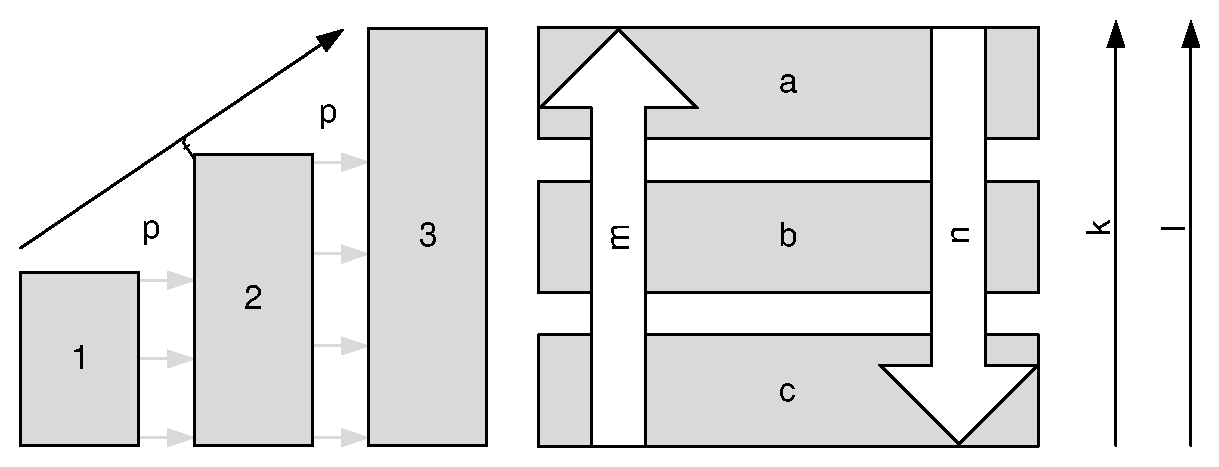
\includegraphics[width=1.0\textwidth]{1_Navigation_Fuehrung_Stabilisierung.eps}
	\caption[Weiterentwicklungstendenzen aus Sicht aktiver Fahreingriffe]{Weiterentwicklungstendenzen aus Sicht aktiver Fahreingriffe dargestellt am Drei-Ebenen-Modell \cite{donges1982aas}}% , vgl.\ \cite{handbuchFAS_Donges2012}}
	\label{fig:Navigation_Fuehrung_Stabilisierung}
\end{figure}

Während die Fahrzeugstabilisierung, vereinfacht gesprochen, von den Ingenieurwissenschaften, und die 
Fahrzeugnavigation (s.\ Abb.\,\ref{fig:Navigation_Fuehrung_Stabilisierung}) 
von der Informatik dominiert wird, überlappen sich beide Disziplinen auf der 
Fahrzeugführungsebene. Grund dafür ist, dass dort das Automobil, ein dynamisches 
System, dessen zielgerichtete Beeinflussung die Aufgabe der Regelungstechnik\index{Regelungstechnik} ist \cite{lunze2005regelungstechnik, unbehauen1989regelungstechnik, foellingeroptimal}, in Interaktion mit seiner Umgebung tritt, welches das Themengebiet der Robotik\index{Robotik} darstellt \cite{Thrun2005,Siciliano2008}. 
Generell befasst sich die Regelungstechnik vor allem mit der Stabilität sowie der Robustheit gegenüber Störungen und Modellfehler eines Systems, beides entscheidende Punkte bei der Funktionsabsicherung von Assistenzsystemen. Die Informatik hingegen widmet sich unter anderem der Lösung stark abstrahierter Probleme mit hoher Komplexität, eine ganz wesentliche Domäne für die "`Intelligenz"' zukünftiger Fahrzeuge \cite{eskandarian2012handbook}. \\
Beide Wissenschaften bedienen sich mathematischer Prinzipien, Methoden und Verfahren, insbesondere aus dem Bereich der Optimierung, die entsprechend der jeweiligen Herangehensweise erfolgreich auf die Fahrzeugführung angewandt wurden. Trotz der thematischen Nähe findet eine direkte Gegenüberstellung, sicherlich erschwert durch die Verwendung unterschiedlicher Fachterminologien, in den seltensten Fällen statt. Gerade aber in einer interdisziplinären Entwicklungsmethodik liegen enorme Chancen, die von Fahrassistenzforschern und "~entwicklern genutzt werden sollten, um modernen Sicherheits- und Komfortsystemen zur Serienreife zu verhelfen.

% Zur Methodik: Optimierung, Graphensuche
% Ing. und Infos kennen oftmals die gegenseitigen Methoden nicht (STabilität: absicherung, Neuplanung, etc.,
% Ingenieure sind stark geprägt durch absicherung: harte Echtzeitanforderungen (roboter darf ruhig mal anhalten um den weg neu zu berechnen.)
% Informatik: Lösungsansätze für komplexe szenarien, Unterschiedliche Begrifflichkeiten) Beispiel mit NMPC und CMU(?)
% Zustandsschätzung der Informatik für best. Probleme überlegen (Patikelfilter, z.B.)
% Unsystematisches Herangehen, Schnittstellen intuitiv gewählt, Aspekte: Modularität, Robustheit
% Ziel: Kombination beider Welten für das Jeweilige Problem
% Planung Informatik: Robotik spezifische intelligente Lösungen
% Planung Regelungstechnik: Stabilität, Störungen, Qualität
% Herausforderung: Freiheitsgrade, Kombinatorik
% Zusammenfassung: Akzeptanz, Kunde, Rechtliche Vorgaben.
%

%Regelungstechnik: 
%- Lehre der Stabilität und Stabilisierung rückgekoppelter dynamischer Systeme
%Rückkopplung ist das wichtigste Grundprinzip der Regelungstechnik
%- Robustheit, Regelgüte, Berücksichtigung oder Kompensation von Störungen, Indentifikation
%
%Mehrebenensteuerung (Lunze I)
%
%Überleitung zu Methoden
%integration bestehender Regelsysteme
%
%Informatik: Millionen von Fahrkombinationen druchspielen

%In Zusammenfassung gilt es, ....

	% Einseitige Bremsung: Spurhalten (Daimler)
% Aktive Lenkeingriffe
	% Unterstützung beim Spurhalten
	% Stauassistenz
% Hinterachslenkung, Torque-Vectoring
% Bei höheren Geschwindigkeiten: Leichte korrigierende Lenkeingriffe zum Spurhalten
%gesteigerten Rechenleistung der Automobilsteuergeräte
% Forschung:
		% 


		
\section{Ziele und Aufgaben}
% Vier Anwendungen: Fzg-Stab: Driften
%										Fzg-Führung + Stab: Anhänger
%										Planung, Führung + Stab: Ausweichen
%            Forschung: NMPC

%	\stich{
% Umfassender Überblick der FAS bzgl. Überschrift, Neuheiten, Konzept zur Bewertung (Bretthauer), Grundsätzliche Motivation für Kapiteleinteilung ohne ins Detail zu gehen \\
%}
Das Hauptziel der vorliegenden Arbeit ist, die Problemstellung aktiver Fahreingriffe derart zu beleuchten, dass Forschungs- oder Entwicklungsteams ein verständlicher Methodenapparat an die Hand gegeben wird, der sie dazu befähigt, neue Sicherheits- und Komfortfunktionen systematisch umzusetzen. Im Einzelnen sind hierzu folgende Teilziele zu erarbeiten: 
\begin{itemize}
	\item Darstellung der Führungs- und Stabilisierungsaufgabe aus Fahrersicht sowie Verdeutlichung der Implikationen für moderne Assistenzsysteme (Kapitel~2)
	\item Übersichtsartige Darstellung der Funktionsweise von Fahrzustands- und Umfelderfassung sowie Aktorik einschließlich ihrer Schnittstellen zum Planungsmodul der Fahreingriffe (Kapitel~2)
%	\item Beschreibung des bestehenden Funktionsumfangs aktueller Fahrerassistenzsysteme der Stabilisierungs- und Führungsebene unter Einbeziehung des abgeleiteten Fahreingriffskonzepts (Kapitel~3 und 4) % Führungsebene: Einparken und Notbremsen
%	\item Vereinheitlichung etablierter Regelungsprinzipien und "~verfahren der automatischen Fahrzeugstabilisierung und Verdeutlichung anhand wichtiger Anwendungsbeispiele aus der Forschungsliteratur (Kapitel~3)
	\item Ableitung eines übergeordneten Fahreingriffskonzepts, welches für typische Assistenzaufgaben das Zusammenspiel von Manöverplanung und "~ausführung einheitlich beschreibt (Kapitel~3)
\item Veranschaulichung mathematischer Methoden zum Nachweis der Durchführbarkeit und Stabilität von Fahrmanövern (Kapitel~3)
	\item Systematisierte Darstellung moderner Manöveroptimierungsmethoden, deren Bewertung hinsichtlich Echtzeitanforderungen und Eignung für verschiedene Einsatzbereiche (Kapitel~4 bis 6) sowie Herausarbeitung von Empfehlungen zu ihrer Kombination (Kapitel~7) 
	%\item Stabilität
	%\item Durchgängige Hinweise auf  und Beispiele zur Implementierung der Methoden und Algorithmen
\end{itemize}
Insbesondere wird durch die hierbei behandelte Materie bei der Beantwortung folgender wichtiger Fragen direkt Hilfestellung gegeben oder auf weiterführende Literatur verwiesen:
\begin{itemize}
%Allgemein: (Kapitel 2)
\item Wann und wie muss ein Sicherheitssystem eingreifen? %Wie wird ein Komfortsystem vorteilhafterweise ein- und ausgeschaltet? 
Wie sieht das Zusammenspiel mit dem Fahrer während des Eingriffs aus? %TTX
\item Wie kann das Fahrzeug über eine seriennahe Sensorik ermitteln, wo es sich befindet oder gerade hinbewegt? Wie ist das Fahrzeugumfeld aus Sicht der Manöverplanung zu repräsentieren? % Odometrie
%\item Was sind die Aufgaben der Planung, was die der Regelung, wie spielen sie zusammen?
%
%Modellierung und Fahrzeugstabilisierung (Kapitel 3)
\item Welche Dynamiken und physikalischen Grenzen des Fahrzeugs einschließlich seiner Aktorik gilt es an welcher Stelle im System zu beachten? Was kann vernachlässigt werden?
\item Welche Störungen und Parameterschwankungen treten in der Praxis auf und wie können sie effektiv kompensiert werden?
%
%Regelung:
\item Wie können Regelziele, "~fehler und "~stellgrößen vorteilhaft definiert werden und wie sind die Schnittstellen zwischen den Einzelsystemen entsprechend zu gestalten?
%\item Welche Regelungsprinzipien und -verfahren haben sich praktisch bewährt?
%\item Vorsteuerung / Regelanteil
%\item Ist die Krümmung eine Störung?
%Planung:
%\item Wie ist das Zusammenspiel mit den restlichen Komponenten?
\item Wie und wo entstehen Rückkopplungen bei der Trajektorienplanung und was muss hierbei beachtet werden?
\item Welche Optimierungskriterien gibt es bei der Planung von Fahreingriffen? Wie können Nebenbedingungen wie Kollisionsfreiheit und fahrphysikalische Grenzen berücksichtigt werden?
%Wie unterscheidet sich die Pfad- von der Trajektorienplanung und wie wirkt sich das auf die Regelung aus?
\end{itemize}

Die Gliederung und die Inhalte der vorliegenden Arbeit orientieren sich am modellprädiktiven Regelkreis\index{Modellprädiktiver Regelkreis} \cite{Lewis_OC}, der vereinfacht in der oberen Hälfte von Abb.\,\ref{fig:Kapiteluebersicht} dargestellt ist. Anhand dessen vermittelt Kapitel~2 die Grundlagen aktiver Fahreingriffe. Während im Anschluss die Stabilität und Robustheit des modellprädiktiven Regelkreises umfassend in Kapitel~3 diskutiert wird, erfolgt die Abhandlung der Fahrzeugführungsaufgabe, also die Trajektorienoptimierung, auf mehrere Kapitel verteilt. Die Gliederung orientiert sich dabei an der klassischen Aufteilung der Methoden zur Lösung dynamischer Optimierungsaufgaben in \emph{Dynamische Programmierung\index{Dynamische Programmierung}, Direkte\index{Direkte Optimierung}} und \emph{Indirekte Optimierungsmethoden\index{Indirekte Optimierung}} (Kapitel~4-6). 
Sie gewinnen bei der Entwicklung von Fahrerassistenzsystemen der Führungsebene weiter an Bedeutung, sodass ihnen der dreifache Kapitelumfang zuteil wird. %Hierbei wird zwischen direkten und indirekten Methoden sowie Methoden der dynamischen Programmierung unterschieden.
Kapitel~7 stellt die wesentlichen Eigenschaften der Optimierungsmethoden gegenüber und gibt ergänzend Empfehlungen zu deren vorteiligen Kombination. Zusätzliche werden dem Neueinsteiger auf dem Gebiet etablierte Handlungshinweisen für die effiziente Erprobung neuer Assistenzfunktionen vermittelt.


\begin{figure}[h]
	\psfrag{a}[cc][cc][1.0]{\parbox[c]{7cm}{\begin{center} Trajektorien- \\ optimierung \end{center}}}
	\psfrag{b}[cc][cc][1.0]{\parbox[c]{7cm}{\begin{center} Unterlagerte \\ Stabilisierung \end{center}}}
	\psfrag{c}[cc][cc][1.0]{\parbox[c]{7cm}{\begin{center} Fahrzeug \end{center}}}
		\psfrag{d}[cc][cc][1.0]{\parbox[c]{7cm}{\begin{center} Messung \\ Zustandsschätzung \end{center}}}
		\psfrag{2}[cc][cc][1.0]{Kap.\,\ref{chap:grundlagen}}
		\psfrag{3}[cc][cc][1.0]{Kap.\,\ref{chap:stabilisierung}}
		%\psfrag{4}[cc][cc][1.0]{Kap.\,\ref{chap:statische_Optimierung}}
		\psfrag{6}[cc][cc][1.0]{Kap.\,\ref{chap:dynamische_Optimierung_direkt}}
		\psfrag{7}[cc][cc][1.0]{Kap.\,\ref{chap:dynamische_Optimierung_indirekt}}
		\psfrag{5}[cc][cc][1.0]{Kap.\,\ref{chap:dynamische_Optimierung_dynamisch}}
		\psfrag{p}[cc][cc][1.0]{\parbox[c]{7cm}{\begin{center} Direkte \\ Methoden \end{center}}}
		\psfrag{q}[cc][cc][1.0]{\parbox[c]{7cm}{\begin{center} Indirekte \\ Methoden \end{center}}}
		\psfrag{o}[cc][cc][1.0]{\parbox[c]{7cm}{\begin{center} Dynamische \\ Programmierung \end{center}}}
		%
		\psfrag{m}[cc][cc][1.0]{\parbox[c]{7cm}{\begin{center} Dynamische \\ Optimierung \end{center}}}
		%\psfrag{n}[cc][cc][1.0]{\parbox[c]{7cm}{\begin{center} Statische \\ Optimierung \end{center}}}
	\centering
  	%\includegraphics[width=1\textwidth,clip, trim = 0cm 0cm 0cm 0cm]
	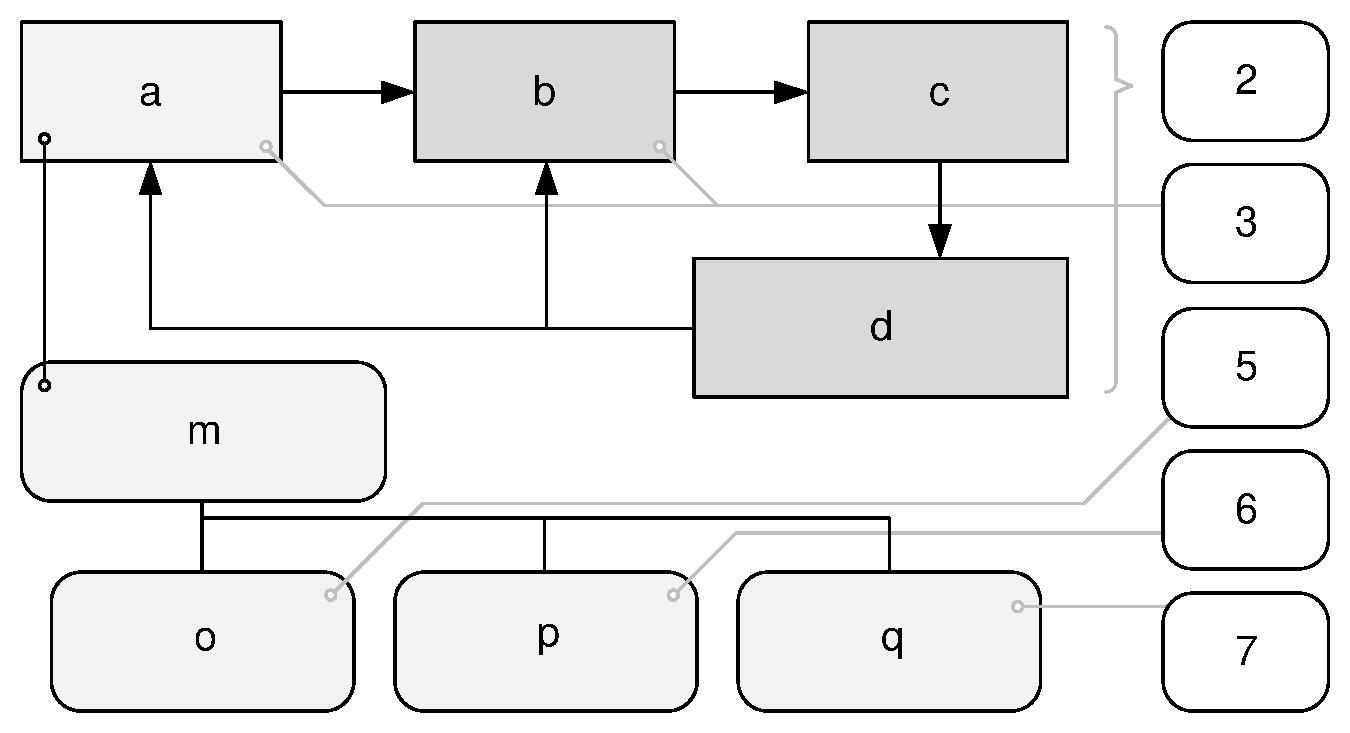
\includegraphics[width=1.0\textwidth]{1_Kapiteluebersicht.eps}
	\caption{Gliederung der Arbeit dargestellt am modellprädiktiven Regelkreis}
	\label{fig:Kapiteluebersicht}%
\end{figure}

Damit gibt die vorliegende Arbeit erstmalig einen systematisierten Überblick zu Methoden, Systemkomponenten sowie deren Verknüpfungen zu Sicherheits- und Komfortsystemen mit aktiven Fahreingriffen. Bei der pädagogischen Themenaufbereitung orientiert sie sich insgesamt an Studenten, Einsteigern und Fortgeschrittenen. Insbesondere bei der Definition der Aufgabenverteilung und dem Zusammenspiel zwischen permanenter Manöveroptimierung und unterlagerter Fahrzeugstabilisierung wird wissenschaftliches Neuland betreten. Darüber hinaus werden neue Algorithmen der Fahrzeugstabilisierungs- und der Fahrzeugführungsebene detailliert hergeleitet und anhand realer Fahrversuche und Simulationen validiert, sodass zusätzlich ein tiefer Einblick in den Kern neuer Assistenzsysteme gegeben wird.

\cleardoublepage

%TODO: % Warnende Systeme haben den Nachteil, dass die Reaktionszeit vom Fahrer hinzukommt. Außerdem muss er dann genau wissen, was er zu tun hat.

% Ideal: je näher in der zukunft desto stärker zählt die physik, je weiter weg, desto eher zähen die Verkehrsregeln und die interaktion

% STVO: gibt heuristiken vor, sodass ics verhindert werdn.

% Selbst wenn die Zukunft genau bekannt ist, ist eine TP, die garantien ausspricht nicht trivial.


%10 Thesen:
%
%Die Anwendungskapitel sind einheitlich aufgebaut, um deren Durcharbeitung zu vereinfachen.
%
%Die Algorithmen der Anwendungsbeispiele sind wissenschaftlich neu.
%
%Alle Anwendungsbeispiele (Kap. 3-7) sind praxiserprobt.
%
%Der Leser erhält sowohl theoretische als auch praktische Aspekte der.
%
%Best-practice mit Hinweisen auf häufig gemachte, zeitraubende Fehler.
%
%Ausgiebige Literaturangaben erleichtern das Folgestudium
	%
	%Sammelwerk aus Methoden der L- und NL-Regelung, welche sich im Automotive-Bereich in der PRAXIS bewährt haben. Dadurch hat der Student die Gewissheit, dass die die Praxistauglichkeit gegeben ist.



	
	%Neben dem obligatorischen ersten und letzten Kapitel, stellen die
%Anwendungskapitel 4, 5, 6 und 7 den Kern der Arbeit dar und sind
%"wissenschaftlich neu". Diese sind so gewählt, dass die beschriebenen
%Funktionen auf aktiven Lenkeingriffen beruhen und die
%Assistenzspektren "Niedriger Unterstützungsgrad" bis "Hoher
%Unterstützungsgrad" sowie "Niedrige Querdynamik" bis "hohe
%Querdynamik" abdecken.
%
%Kapitel 4 stellt die Erweiterung des automatischen Einparkens auf
%Fahrzeuge mit Anhänger dar. Es werden zwei Regler entworfen, die es
%ermöglichen, entweder nur den Knickwinkel des Anhängers zu
%stabilisieren, was die permanente Anpassung der Sollvorgabe vom Fahrer
%erfordert, oder dass das Fahrzeug eigenständig einen geometrischen
%Pfad stabilisiert (z.B. Einparken). Hierzu bereite ich gerade einen
%at-Beitrag vor.
%
%Kapitel 5 demonstriert, wie mit Hilfe der Lenkung (und nicht wie
%herkömmlich mit Einzelradbremsungen) ein schleuderndes Fahrzeug
%abgefangen oder (für Fahrertrainingszwecke) absichtlich unter
%Zuhilfenahme des Motormoments im Driften gehalten werden kann. Im
%Unterschied zu bisherigen Arbeiten ist das Besondere hierbei, dass der
%Regler als Parameter ausschließlich die Lenkübersetzung braucht
%(robuster Sliding-mode-Regler) und nur die Seriengierrate rückführt.
%Eine Veröffentlichung ist in Arbeit.
%
%Kapitel 6 stellt eine algorithmisch unbedeutende, für die Praxis aber
%umso wichtigere Funktion dar, welche Kollisionen im Seitenbereich
%(Spurwechsel mit Fahrzeug im Toten Winkel) verhindert. Hierzu wird,
%wie auch im nächsten Kapitel, auf die Fahrzeugumfeldsensorik
%zurückgegriffen.
%
%Kapitel 7 wird den größten Umfang haben, da hier mein
%Forschungsschwerpunkt liegt. Ich beschränke mich auf zwei Ansätze der
%Optimalsteuerung. Der indirekte Ansatz zeichnet sich durch schwer zu
%unterbietende Rechenzeiten aus, sodass dieser auf aktuellen
%Steuergeräten problemlos umgesetzt werden.
%Bei Kombination mit Bremsmanövern bekommen die fahrphysikalischen
%Restriktionen und die Fahrzeug-Nichtlinearitäten ein höheres Gewicht,
%sodass diesen mit einem direkten Ansatz, der nichtlinearen
%modellprädiktiven Regelung, begegnet wird. Für letzteres ist das Paper
%auf der CDC angenommen worden.
%
%Da sich die verwendeten Methoden auf andere Assistenzsysteme anwenden
%lassen, die aus Platzgründen nicht beschrieben sind (und mit denen ich
%mich, bzw. mein Doktorand, auch erst in Zukunft beschäftigen werde),
%und um die Anwendungskapitel leserlich zu gestalten, habe ich die
%Regelungsmethoden in Kapitel 3 vorverlagert.
%
%Das davor befindliche Kapitel 2 beinhaltet schließlich neben den von
%mir angesammelten "best-practice" Erfahrungen, weitere wertvolle
%Grundlagen (auf die im Anschluss zurückgegriffen wird), sodass der
%Leser einen guten Überblick über alle wichtigen Begriffe der Hartware-
%und Softewarekomponenten sowie deren Bedeutung für die
%Fahrerassistenzforschung bekommt.
%


	
	
%Mit Achsen:
%----------------------------- niedrige Fahrdynamik ------------- hohe Fahrdynamik --
%hoher     Unterstützungsgrad:	[1 Rangierassistenz]  						 [2 Driftassistenz]
%niedriger Unterstützungsgrad: [3 LCA]               						 [4 Kombinierte Brems-Ausweich-Assistenz/Integrierte Kollisionsvermeidung]           
%hoher Unterstützungsgrad:     permanent
%niedriger Unterstützungsgrad: kurzzeitig (keine Aussage über Wirksamkeit!), haptische Untersützung, kein Anspruch auf eigenständiges Lenken.
%
%niedrige Fahrdynamik/Querdynamik: 				kaum Querbeschleunigung oder Schräglaufwinkel
%hohe Fahrdynamik/Querdynamik: 						erhebliche Querbeschl. oder Schräglaufwinkel
%
%
									%
%
%Mit Beschriftung							
%----------------------------- Komfort ---------------- Sicherheit --
%Lenken alleine:			        [1 Rangierassistenz]  		[3 LCA, falls kein Bremseingriff]
%Kombination mit Gas/Bremse: [2 Driftassistenz]        [4 Kombinierte Brems-Ausweich-Assistenz/Integrierte Kollisionsvermeidung


\chapter{Problemstellung aktiver Fahreingriffe} \label{chap:grundlagen}

%\zitat{But in science the credit goes to the man who convinces the world, \\
%not to the man to whom the idea first occurs.}{Sir Francis Darwin}
\zitat{Es ist nicht genug, zu wissen, man muss auch anwenden; \\
es ist nicht genug zu wollen, man muss auch tun.} {Johann Wolfgang von Goethe}



% Was soll in diesem Kapitel gemacht werden?

In vielen automatisierungstechnischen Anwendungen kommen sog.\ Mehrschicht-\index{Mehrschichtsteuerung} bzw. Mehrebenensteuerungen\index{Mehrebenensteuerung} \cite{lunze2005regelungstechnik} zum Einsatz, die auf dem Prinzip der Dekomposition und Koordination komplexe Aufgabenstellungen\footnote{Als Beispiel sei eine Ablaufsteuerung genannt, die entsprechend einem optimierten Prozess-Grobschema entworfen wird, sodass in Abhängigkeit des aktuellen Prozessschritts eine gezielte Anpassung der nachgeschalteten Steuer- oder Optimierungsalgorithmen erfolgt. Letztere können dann wiederum nach konkretisierten Maßgaben zwischen verschiedenen Sensoren und Aktoren umschalten.%, sodass schließlich, nach dem Durchlauf des Grobschemas, das eigentliche Resultat der Automation erreicht wird.
}  lösen \cite{reinisch1974kybernetische}. Aufgrund hoher Anforderungen an die Funktionsrobustheit und -qualität stellen Fahrerassistenzsysteme hier keine Ausnahme dar. \\
Die Unterteilung moderner Assistenzfunktionen in geeignete Hierarchieebenen ist jedoch keinesfalls trivial, da sie immer von Kompromissen begleitet wird. Infolgedessen wird im vorliegenden Kapitel zunächst das menschliche Verhalten in Form eines etablierten Fahrermodells beschrieben und dazu regelungstechnische Parallelen gezogen. Hierbei stellt sich heraus, dass die Trajektorienoptimierung des Fahrmanövers eine zentrale Rolle einnimmt, da sie nicht nur optimale Fahrzeugbewegungen berechnet, sondern auch durch die Rückführung des Fahrzeug-Istzustands eine qualitativ hochwertige Stabilisierung realisiert. Aufgrund von Einschränkungen bei der praktischen Umsetzung aktorischer Eingriffe ist jedoch in jedem Fall die Trajektorienoptimierung mit einer unterlagerten Regelung zu kombinieren, was später genauer erläutert wird. \\
Der Entwurf und die Umsetzung aktiver Fahreingriffe erfordert generell ein breites Verständnis über die der Fahrerassistenzfunktion zur Verfügung stehenden Schnittstellen zur Aktorik und Sensorik, da erst so das volle Potential bestehender Fahrzeugarchitekturen ausgeschöpft werden kann. Viel wichtiger noch: Sind die grundsätzlichen Zusammenhänge zwischen Eingangs- und Ausgangsdaten verstanden, befähigt das den Entwickler einer Fahrerassistenzfunktion, bei auftauchenden Problemen mit dem jeweiligen Schnittstellenpartner konstruktiv Verbesserungen zu erarbeiten, die das Gesamtsystem auf eine höhere Leistungsebene heben. Aus diesem Grund werden die für die Fahrerassistenzfunktion wichtigsten Aspekte der hinter den etablierten Schnittstellen befindlichen Hardware- und Softwarekomponenten genauer betrachtet. Dabei wird, wann immer möglich, eine zukunftsgerichtete Perspektive eingenommen. \\ %der Schwerpunkt auf zukunftsträchtige Fahrzeugtechnologien gelegt wurde.
%
Ausgangsseitig gehören zu den Schnittstellensystemen die elektromechanische Servolenkung, das elektrohydraulische Bremssystem und der Fahrzeugantrieb. Eingangsseitig handelt es sich um das Sensorcluster (bestehend aus Drehraten- und Beschleunigungssensoren), die Geschwindigkeits- und Schwimmwinkelschätzung, die Module der lokalen und globalen Eigenlokalisierung sowie die Fahrzeugumfeld-Erfassung und -Prädiktion. \\
Abschließend wird im Kapitel die grundsätzliche Herangehensweise bei der Systemaktivierung von Assistenzfunktionen erläutert. Hierzu wird auf das Konzept der sog.\ \emph{Systemzustände einer unvermeidlichen Kollision} und darauf aufbauende subjektive Kritikalitätsmaße zurückgegriffen.
	
	
% Für ein tiefgründiges Verständnis ist es wichtig, auch die unterlagerten Regler zu kennen, die zu einer Beeinflussung des Fahrzeugs führen. Da damit immer eine Dynamik einher geht, die je nach Anwendungsfall vernachlässigt werden kann oder nicht, ist es wichtig auch die physikalischen Zusammenhänge grob zu verstehen.
% -> Übergeordnete Betrachtung, welche sich durch alle anschließenden Kapitel zieht.
%
%Mehrebenen-Optimierung





% Begründung für Schwierigkeit am Beispiel einer Heizung: Hohe Koppelung zwischen Regelung und Führung (nicht so wie Heizungssystem)

\section{Klassifikationsschema der menschlichen Fahraufgabe\index{Fahraufgabe}}

\subsection{Drei-Ebenen-Modell} \label{sec:drei-ebenen-modell}
Entsprechend \cite{handbuchFAS_Donges2012} besteht die übergeordnete Aufgabe des Fahrers darin, das Kraftfahrzeug mit Hilfe von Fahreingriffen unter Berücksichtigung der verfügbaren Information sicher an einen Zielort zu überführen. Eine Unterteilung in hierarchisch verknüpfte Einzelaufgaben kann über das Drei-Ebenen-Modell erfolgen \cite{donges1982aas}, das bereits in der Einleitung in Abb.\,\ref{fig:Navigation_Fuehrung_Stabilisierung} herangezogen wurde und starke Ähnlichkeit mit einem kaskadierten Regelkreis\index{Kaskadenregelung} \cite{graf2003neue} aufweist, s.\ Abb.\,\ref{fig:dreiebenenmodell}. Hierbei umfasst die \textbf{Navigationsaufgabe}\index{Navigationsebene} die Bestimmung einer optimalen Fahrroute in Abhängigkeit des aktuellen Fahrzeugortes und der momentanen Verkehrslage zu diskreten Zeitpunkten, wie zum Fahrtantritt oder Befund einer Straßensperrung. Die Umsetzung der Fahrroute in konkrete Fahrmanöver ist Aufgabe der nachgeschalteten \textbf{Führungsebene}\index{Führungsebene}. Sie wählt unter Berücksichtigung der aktuellen Fahrzeugposition und -bewegung sowie des prädizierten Fahrraums  unter vielerlei Gesichtspunkten, wie Komfort, Verbrauch und Verkehrssicherheit, das zukünftige Fahrmanöver aus. Dessen Realisierung erfolgt mittels motorischer Eingriffe in Lenkrad und Pedalerie und wird aufgrund der hierbei zu unterdrückenden Störungen als \textbf{Stabilisierungsaufgabe}\index{Stabilisierungsebene} bezeichnet. 


%
%
\begin{figure}[h]
	\newcommand{\smallsize}{.85}
	\psfrag{1}[cc][cc][\smallsize]{Navigation}
	\psfrag{2}[cc][cc][\smallsize]{Führung}
	\psfrag{3}[cc][cc][\smallsize]{\parbox[c]{7cm}{\begin{center}Stabilisierung \end{center}}}
	%
	\psfrag{4}[cc][cc][\smallsize]{\parbox[c]{7cm}{\begin{center}Straßennetz \end{center}}}
	\psfrag{5}[cc][cc][\smallsize]{Fahrraum}
	\psfrag{6}[cc][cc][\smallsize]{Fahrzeug}
	%
	\psfrag{7}[cc][cc][\smallsize]{\parbox[c]{7cm}{\begin{center}Lenkung u. \\ Pedalerie \end{center}}}
	%
	\psfrag{m}[cc][cc][1.0]{Planungshorizont}
	\psfrag{n}[cc][cc][1.0]{Reaktionsschnelligkeit}
	%
	\psfrag{a}[cc][cc][1.0]{Fahrer}
	\psfrag{b}[cc][cc][1.0]{Umwelt}
	\psfrag{d}[cc][cc][1.0]{Stellglieder}
	\psfrag{c}[cc][cc][1.0]{Strecke}
	%
	\psfrag{w}[bc][bc][\smallsize]{Fahrzustand 1}
	\psfrag{x}[bc][bc][\smallsize]{Fahrzustand 2}
	\psfrag{y}[bc][bc][\smallsize]{Verkehrsteilnehmer, Hindernisse und relative Fahrspurposition}
	\psfrag{z}[bc][bc][\smallsize]{Aktuelle Fahrspur und Geschwindigkeit}
	\centering
	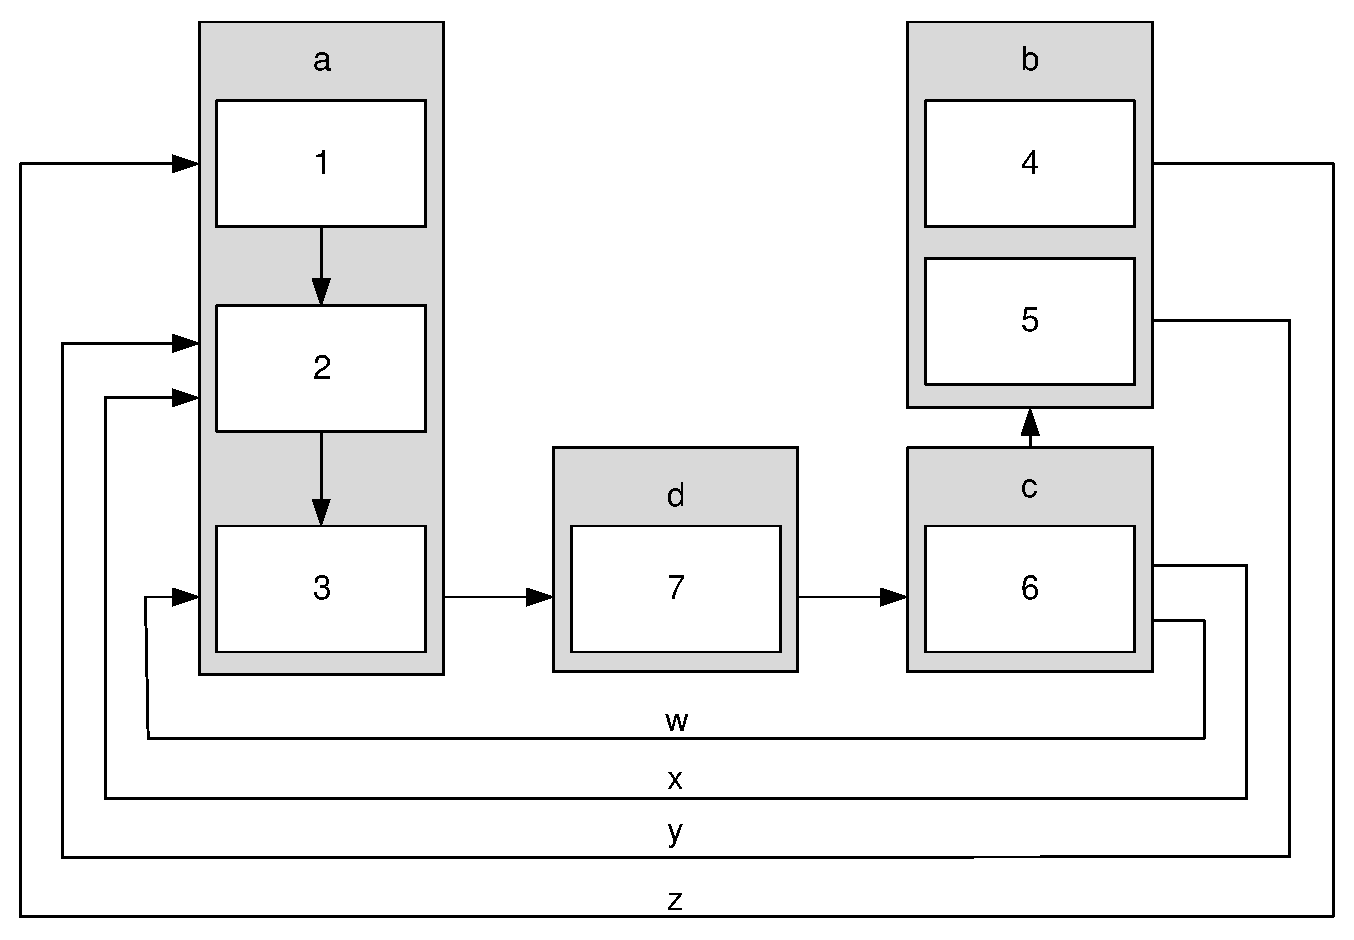
\includegraphics[width=1.0\textwidth]{2_3-Ebenen-Modell.eps}
	\caption[Modifiziertes Drei-Ebenen-Modell]{Für kritische Fahrsituationen und erfahrene Fahrzeugführer modifiziertes Drei-Ebenen-Modell, vgl.\ \cite{donges1996regelsysteme}}% , vgl.\ \cite{handbuchFAS_Donges2012}}
	\label{fig:dreiebenenmodell}
\end{figure}

Abweichend von der Darstellung des Fahrzeugnormalbetriebs in \cite{handbuchFAS_Donges2012} wird in Abb.\,\ref{fig:dreiebenenmodell} den besonderen Anforderungen bei kritischen Fahrmanövern wie dem Ausweichen Rechnung getragen. Sie verlangen dem Fahrer auf der Führungsebene nicht nur eine genaue Manöverplanung ab, sondern auch eine permanente Berücksichtigung bestimmter Komponenten des aktuellen Fahrzustands (Fahrzustand 2). 
%Letzteres bedarf einer zusätzlichen Erklärung: 
Beim Spurhalten im Normalbetrieb werden nämlich, ungeachtet des Fahrzeugzustands, von der Führungsebene lediglich die Sollspur und die Sollgeschwindigkeit an die Stabilisierungsebene weitergeleitet, die dann Abweichungen von den Sollvorgaben minimiert. Während eines fahrphysikalisch anspruchsvollen Manövers hingegen, muss der Fahrer auf der Führungsebene darauf Rücksicht nehmen, wie sein %durch die Stabilisierungsebene geregeltes 
Fahrzeug tatsächlich reagiert. Das setzt ein gutes Fahrgefühl\footnote{Ein im deutschsprachigen Automobilsport verbreiteter, scherzhafter Ausdruck ist hierfür das sog.\ \emph{Popometer}.} für den Fahrzeugzustand und die Fahrbahnbeschaffenheit voraus. 
Bei rutschigem Untergrund beispielsweise folgt das Fahrzeug häufig nicht so schnell der Lenkbewegung wie erwartet, sodass ein ungeübter Fahrer versucht ist, durch weiteres Einlenken auf der ursprünglichen Ausweichtrajektorie zu bleiben und dadurch eine Verstärkung des sog.\ \emph{Untersteuerns}\index{Untersteuern} riskiert. Der geübte Fahrer hingegen erkennt frühzeitig, dass sein Fahrzeug "`über die Vorderräder schiebt"' und korrigiert das Manöver unter Berücksichtigung des aktuellen Fahrzustands % sowie der geschätzten Fahrbahnbeschaffenheit 
auf der Führungsebene.  Hierdurch entscheidet er sich u.\,U. für ein zum Hindernis hin knapperes, dafür aber fahrphysikalisch realisierbares Ausweichmanöver, mit dem er eine Kollision erfolgreich vermeidet.
Das lässt vermuten, dass der Fahrer mit steigender Erfahrung einen immer größeren Teil des Fahrzustands auf der Führungsebene berücksichtigt.

\subsection{Regelungstechnische Betrachtungsweise}
Aus regelungstechnischer Sicht wird der Fahrer bei seiner Fahraufgabe in jedem Zeitschritt mit einem  Optimalsteuerungsproblem\index{Optimalsteuerung} \cite{foellingeroptimal} konfrontiert, vgl.\ \cite{prokop2001modeling, preusse2001fahrzeugfuhrung}, dessen permanente Lösung bei Berücksichtigung des aktuellen Fahrzustands und der Umgebungsinformation zu einer Stabilisierung des Gesamtsystems führt (s.\ später \abschn{sec:begriffe}).
Das zugrunde gelegte Optimierungskriterium setzt sich i.\,Allg.\ aus Fahrzeit, Verbrauch, Komfort und Sicherheit zusammen. Im Sinne der Optimierungsnebenbedingungen ist zusätzlich zur Fahrphysik auch die jeweils geltende Straßenverkehrsordnung einzuhalten. Die Lösungsfindung einer so abstrakten Aufgabenstellung erfordert jedoch auch vom Menschen die eingangs angesprochene Dekomposition in spezifizierte Teilaufgaben und motiviert das Drei-Ebenen-Modell des vorherigen Abschnitts. Dieses gilt es nun unter dem Aspekt der Optimierung genauer zu beleuchten.

% (unendlichdimensionalen\footnote{Es existieren unendliche viele Möglichkeiten, ein Fahrzeug von A nach B überzuführen.})

In der Mathematik werden bei einem sog.\ Multi-level-Optimierungsansatz große Probleme hierarchisch abstrahiert und in den dabei entstehenden Subproblemen nach teils unterschiedlichen Kriterien optimiert. Auch die Regelungstechnik macht sich die Herangehensweise bei der zuvor erwähnten Mehrebenensteuerung zunutze \cite{lunze2005regelungstechnik}. Sie adressiert damit gleichzeitig drei wichtige und mit den ihr auferlegten Echtzeitanforderungen unmittelbar verknüpfte Aspekte: den Optimierungshorizont\index{Optimierungshorizont}\footnote{Zeitintervall in die Zukunft, auf dem das Streckenverhalten betrachtet wird.}, die Zykluszeit\index{Zykluszeit}\footnote{Verstreichende Zeitspanne bis in der Optimierung die neue Messinformation Berücksichtigung findet.} und die Systemzustandsdimension\index{Systemzustand}\footnote{Anzahl der dem Optimierungsproblem zugrunde gelegten Modell-Systemzustände}. Ein weitreichender Optimierungshorizont ist für das Auffinden einer langfristig guten Strategie erforderlich und sollte sich an den langsamsten Dynamiken der Strecke orientieren. Die Systemstabilität des durch die Zustandsrückführung in der permanenten Optimierung geschlossenen Regelkreises hingegen verlangt eine so kurze Zykluszeit, dass auch die schnellsten Streckendynamiken berücksichtigt und damit robust stabilisiert werden können. Aufgrund der beschränkten Rechenleistung eines jeden Computers steht aber ein langer Optimierungshorizont mit einer kurzen Zykluszeit im Widerspruch. %\footnote{Eine Ausnahme stellen sog.\ Linear-quadratische-Probleme dar, s.\ Abschn.\,\ref{sec:lqr}, deren Lösung trotz eines unendlichen Optimierungshorizonts eine kontinuierliche Rückführung ermöglichen.}, 
Er kann durch eine hierarchische bzw.\ kaskadische Problemaufteilung, wenn auch kompromissbehaftet, aufgelöst werden, indem in der Signalkette sukzessive immer mehr Zustände des Fahrzeugs berücksichtigt werden. \\
Konkret spiegelt sich das im Drei-Ebenen-Modell darin wider, dass auf \textbf{Navigationsebene}\index{Navigationsebene}
\begin{itemize}
\item die Fahrzeit und der Verbrauch optimiert werden, 
\item die Fahrphysik zu vernachlässigen ist (Abstraktion auf Punktbewegung), 
\item sich die Zykluszeit auf wenige Optimierungen pro Minute beschränkt und 
\item sich der Optimierungshorizont über mehrere Stunden erstrecken kann. 
\end{itemize}
Das Ergebnis ist eine Fahrroute, welche der Optimierung auf Fahrzeugführungsebene als Referenz dient und weiter verfeinert werden muss. \\
Die \textbf{Fahrzeugführungsebene}\index{Fahrzeugführungsebene} wiederum setzt sie nach Möglichkeiten um und optimiert dabei die zukünftige Fahrzeugbewegung
\begin{itemize}
\item unter Sicherheits- und Komfortaspekten (primär),
\item unter Berücksichtigung der Fahrphysik,
\item auf einem Optimierungshorizont von wenigen Sekunden, 
\item dafür aber so häufig wie möglich, um schnell auf den veränderlichen Verkehr und den Fahrzeugzustand reagieren zu können.
\end{itemize}
%um der schnell wechselnden Fahrsituation Rechnung zu tragen. 
Das Resultat stellt ein optimiertes Fahrmanöver dar, das von der \textbf{Stabilisierungsebene}\index{Fahrzeugführungsebene} trotz Modellunsicherheiten hinreichend genau mittels Eingriffen in die Fahrzeugquer- und -längsdynamik auszuführen ist.

Da sowohl auf der Stabilisierungsebene als auch auf der darüber liegenden Führungsebene der Fahrzeugzustand rückgeführt wird, übernimmt auch die Führungsebene einen Teil der Stabilisierungsaufgabe. 
Um etwaige Wechselwirkungen innerhalb der Module eines Fahrerassistenzsystems erkennen und beurteilen zu können, wird die Thematik noch genauer in Kapitel~\ref{chap:stabilisierung} beleuchtet. %mit einem allgemeinen regelungstechnischen Fokus 
%Die mathematische Behandlung der Stabilität modellprädiktiver Regelkreise erfolgt dann in 

\section{Begriffserläuterungen der Regelungstechnik und Robotik} \label{sec:begriffe}
Im Kontext moderner Fahrerassistenzsysteme häufig anzutreffende Termini sind \emph{Trajektorien-}\index{Trajektorienplanung} und \emph{Pfadplanung}\index{Pfadplanung},  welche der Regelungstechnik und Robotik entstammen. Da die vorliegende Arbeit ihren Fokus auf die Optimierung auf Fahrzeugführungsebene legt, soll an der Stelle dem Leser deren Ursprungsgedanke vermittelt und ein Überblick über eng damit verbundene Begrifflichkeiten verschafft werden. Es sei jetzt schon angemerkt, dass in der Fachliteratur aufgrund unterschiedlicher Forschungsschwerpunkte die Verwendung der Begriffe nicht einheitlich erfolgt.
%Darauf aufbauend wird anschließend das für die Praxisanwendung wichtige Zusammenspiel von Optimierung und Regelung genauer beleuchtet.
\subsection{Trajektorien- und Pfadplanung} \label{sec:begriff_tp}
% Oft nicht optimal, einmalig und impliziert damit nachgelagerte Reglung
Die industrielle Praxis der Regelungstechnik ist geprägt von sog.\ Arbeitspunkten und deren Wechsel \cite{lunze2005regelungstechnik, hagenmeyer2004flachheitsbasierter}. Hierbei wird über eine lange Zeit hinweg eine konstante Referenz vorgegeben, deren Stabilisierung Aufgabe der Regelung ist (\emph{Festwertregelung}). Wird nun zwischen weit auseinander liegenden Arbeitspunkten abrupt umgeschaltet, so läuft der Regler Gefahr, in die (im Reglerentwurf oftmals unmodellierten) Stellgrößenbeschränkungen zu laufen, sodass sich die Strecke destabilisiert (\emph{Regler-} bzw.\ \emph{Strecken-Windup} \cite{hippe2004neue}). Zur Vermeidung solcher Effekte %der mit solchen Arbeitspunktwechseln verbundenen Stöße auf die Strecke und möglicherweise gar auftretenden Destabilisierung des Regelkreises , 
wird der zeitliche Sollverlauf der Führungsgröße zwischen den Arbeitspunkten entsprechend der verfügbaren Stellgröße gewählt \cite{hagenmeyer2004flachheitsbasierter} und die Festwertregelung\index{Festwertregelung} durch eine (asymptotische) \emph{Folgeregelung}\index{Folgeregelung} ersetzt, s.\ \abb{fig:arbeitspunktwechsel_tp_prinzip}. Zur Beschreibung des Sollverlaufs $\bs x_r(t)$ (hier für den Systemzustand) reicht häufig ein Referenzpolynom entsprechender Ordnung, bei dem die Transitionszeit $T_\text{trans}$ so minimiert wird, dass die Beschränkungen für die Stellgröße $\bs u$ (in Abb.\,\ref{fig:arbeitspunktwechsel_tp} auf $\bs u_{\min}$) nicht aktiv werden, s.\ \zB \cite{zeitz2010differenzielle}. %Im Allgemeinen kommen dabei Methoden der Parameteroptimierung zum Einsatz, was auch als Statische Optimierung \cite{foellingeroptimal} bezeichnet wird. %, s.\ Kap.\,\ref{chap:statische_Optimierung}.
%Die Stabilisierung der sich zeitlich verändernden Referenztrajektorie $x_r(t)$ wird über eine nachgelagerte Folgeregelung \cite{hagenmeyer2004flachheitsbasierter} realisiert, s.\ hierzu später Abschn.\ref{todo}. 
Bemerkenswert ist an der Stelle, dass keine Rückkopplung des Systemzustands~$\bs x$ auf der Planungsebene stattfindet, mit Ausnahme der Systeminitialisierung (s.\ $\bs x_0$ in \abb{fig:arbeitspunktwechsel_tp_prinzip}), etwa beim Anfahren. Mit anderen Worten: Die Trajektorienplanung verlässt sich darauf, dass die unterlagerte Regelung korrekt arbeitet.\\
Der Begriff "`Planung"' impliziert jedoch keinesfalls, dass immer eine Optimierung stattfindet. Für einfache Problemstellungen reicht es nämlich aus, die funktionale Darstellung des Übergangs $\bs x_r(t)$ so zu wählen, dass nach Festlegung der Stetigkeitsanforderung und Transitionszeit kein Freiheitsgrad für eine Optimierung verbleibt. Erfordert die regelungstechnische Aufgabenstellung jedoch eine (möglicherweise zyklische) Optimierung, impliziert die Verwendung des Begriffs "`Trajektorienplanung"' dann \iA den Einsatz einer \emph{nachgelagerten} Folgeregelung, s.\ Absch.\,\ref{sec:asymptotische_folgeregelung}.\\

\begin{figure}[h]
\newcommand{\smallsize}{.85}
	\psfrag{1}[cr][cr][1.0]{$\bs x(t)$}
	\psfrag{2}[tc][tc][1.0]{$t$}
	\psfrag{u}[cr][cr][1.0]{$\bs u(t)$}
	\psfrag{m}[cr][cr][1.0]{$\bs u_{\min}$}
	\psfrag{a}[cc][cc][\smallsize]{\parbox[c]{7cm}{\begin{center}Trajektorien-\\ planung \end{center}}}
	\psfrag{b}[cc][cc][\smallsize]{\parbox[c]{7cm}{\begin{center}Folge-\\ regelung \end{center}}}
	\psfrag{c}[cc][cc][\smallsize]{\parbox[c]{7cm}{\begin{center}Strecke \end{center}}}
	\psfrag{x}[bc][bc][1.0]{$\bs x_r$}
	\psfrag{r}[bc][bc][1.0]{$\bs u$}
	\psfrag{z}[bc][bc][1.0]{$\bs x$}
	\psfrag{y}[cl][cl][1.0]{$\bs x_0$}
	\centering
	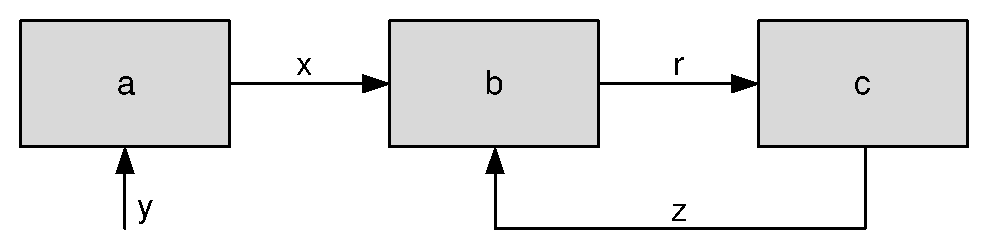
\includegraphics[width=.8\textwidth,clip, trim = 0cm 0cm 0cm 0cm]{2_Prinzip_Trajektorienplanung.eps} \\
	  	\caption{Arbeitsweise einer Trajektorienplanung mit Folgeregelung}
    \label{fig:arbeitspunktwechsel_tp_prinzip}
\end{figure} 
%
\begin{figure}[h]
\newcommand{\smallsize}{.85}
	\psfrag{1}[cr][cr][1.0]{$\bs x(t)$}
	\psfrag{2}[tc][tc][1.0]{$t$}
	\psfrag{u}[cr][cr][1.0]{$\bs u(t)$}
	\psfrag{m}[cr][cr][1.0]{$\bs u_{\min}$}
	\psfrag{T}[bc][bc][1.0]{$T_\text{trans}$}
	\psfrag{a}[cc][cc][\smallsize]{\parbox[c]{7cm}{\begin{center}Trajektorien-\\ planung \end{center}}}
	\psfrag{b}[cc][cc][\smallsize]{\parbox[c]{7cm}{\begin{center}Folge-\\ regelung \end{center}}}
	\psfrag{c}[cc][cc][\smallsize]{\parbox[c]{7cm}{\begin{center}Strecke \end{center}}}
	\psfrag{x}[bc][bc][1.0]{$\bs x_r$}
	\psfrag{r}[bc][bc][1.0]{$\bs u$}
	\psfrag{z}[bc][bc][1.0]{$\bs x$}
	\psfrag{y}[cl][cl][1.0]{$\bs x_0$}
	\centering
  	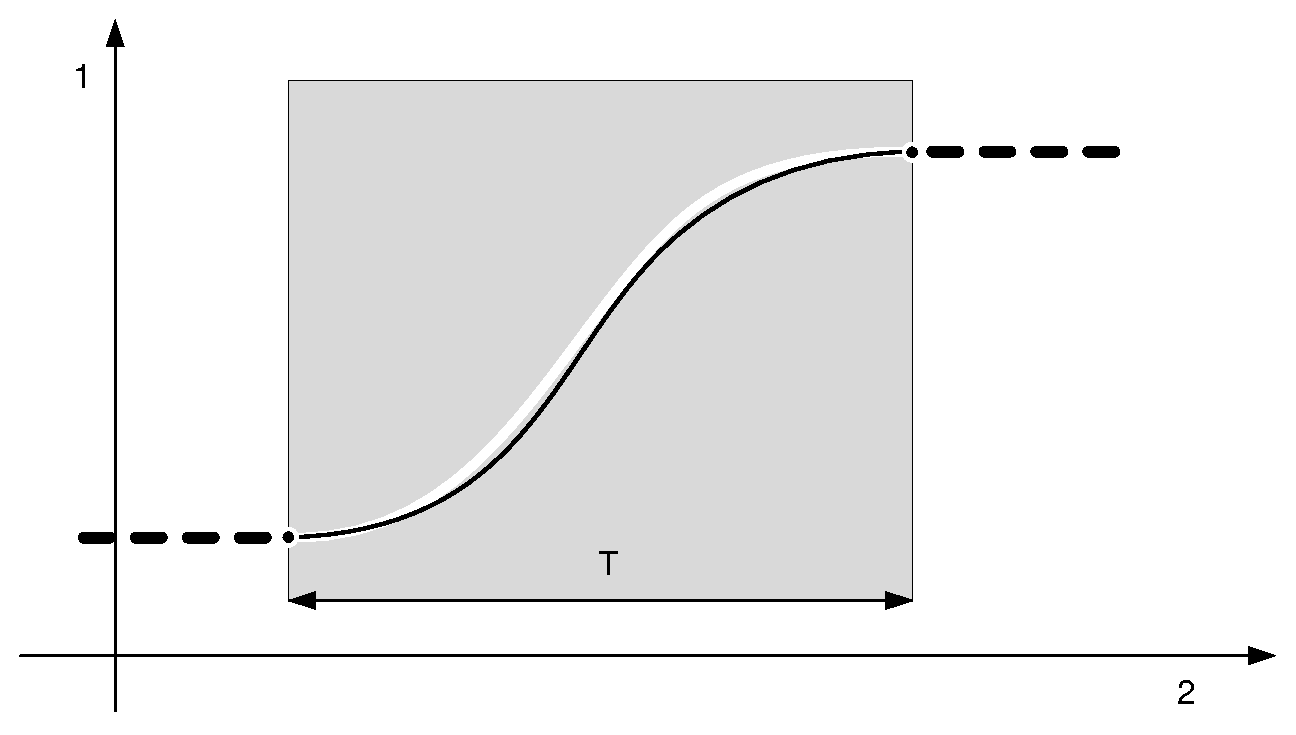
\includegraphics[width=.47\textwidth,clip, trim = 0cm 0cm 0cm 0cm]{2_arbeitspunktwechsel_tp.eps} 
	\hspace{.5cm}
		 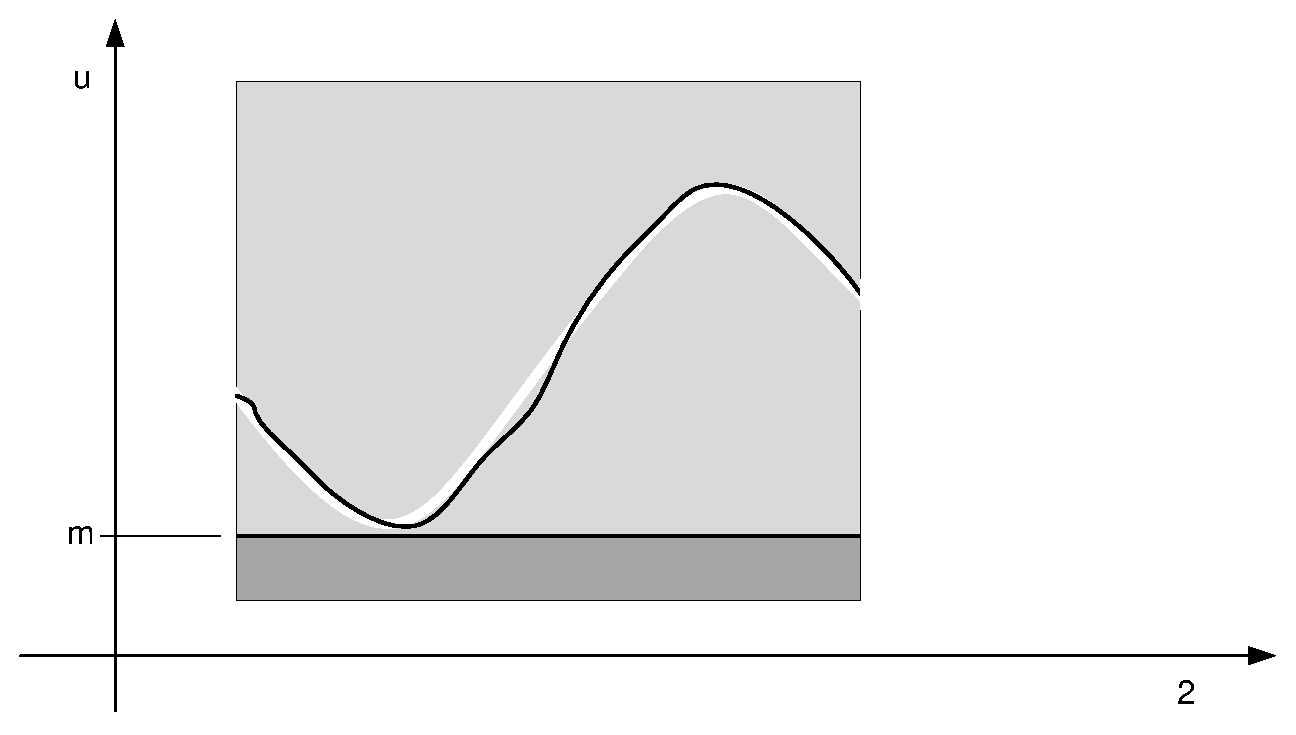
\includegraphics[width=.47\textwidth,clip, trim = 0cm 0cm 0cm 0cm]{2_arbeitspunktwechsel_tp_u.eps}
  	\caption[Signalverläufe bei der Trajektorienplanung]{Signalverläufe eines Arbeitspunktwechsels bei der Trajektorienplanung mit Folgeregelung: Geplante Referenzverläufe des Zustands und der Stellgröße in Weiß, tatsächliche Verläufe in Schwarz; $T_\text{trans}$ bezeichnet die Transitionszeit zwischen den Arbeitspunkten und $\bs u_{\min}$ die (untere) Stellgrößensättigung}
    \label{fig:arbeitspunktwechsel_tp}
\end{figure}
Die Robotik verwendet den Begriff "`Trajektorienplanung"' jedoch in einem etwas anderen Kontext. Häufig kann die Roboterumgebung als statisch angesehen werden, sodass die Zeit $t$ eine untergeordnete Rolle spielt. Wenn nämlich die Roboterdynamik weitgehend geschwindigkeitsunabhängig ist, dann kommt es vielmehr auf die richtige Abfolge der Stelleingriffe an (häufig in Abhängigkeit der zurückgelegten Wegstrecke $s$, welche dann die unabhängige Variable darstellt), und es wird von \emph{Pfad-}\index{Pfadplanung} oder \emph{Bahnplanung}\index{Bahnplanung} gesprochen \cite{latombe1990robot, lavalle2006pa}. Der Begriff "`Trajektorienplanung"' wird nur dann herangezogen, wenn das Planungsergebnis in Abhängigkeit von der Zeit vorliegt. Im einfachsten Fall reicht es hierfür aus, den Pfad mit einem Geschwindigkeitsprofil zu überlagern \cite{lavalle2006pa}.

%Auch wenn hierbei häufig von $t$ zu einer anderen unabhängigen Variablen wie der auf dem berechneten Pfad zurückgelegten Wegstrecke $s$ übergegangen wird, ändert sich grundsätzlich nichts an den zuvor beschriebenen Problemstellungen und Herangehensweisen. Lediglich die Stabilisierung des Manövers erfordert in bestimmten Situationen zusätzlich die Bestimmung des aktuellen $s$ durch Projektion (s.\ hierzu später Abschn.\ref{sec:projektion}).




\subsection{Optimalsteuerung} \label{sec:def_optimalsteuerung}
Treten beim Arbeitspunktwechsel zu den Stellgrößenbeschränkungen\index{Stellgrößenbeschränkung} zusätzlich Gütekriterien wie die Minimierung der Stellenergie hinzu, oder soll die verfügbare Stellgröße besser ausgenutzt werden, um die Transitionszeit weiter zu verkürzen, so wird in der Regelungstechnik die Methode der \emph{Optimalsteuerung}\index{Optimalsteuerung} \cite{foellingeroptimal} angewandt\. %, s.\ Kap.\,\ref{chap:dynamische_Optimierung_direkt}, \ref{chap:dynamische_Optimierung_indirekt} und \ref{chap:dynamische_Optimierung_dynamisch}.  %\footnote{Viele numerischen Methoden der dynamischen Optimierung approximieren allerdings das Problem durch ein Optimierung eingesetzt}.
Im Mittelpunkt steht hierbei die Optimierung des Modellverhaltens als Reaktion auf das Systemeingangssignal $\bs u$. Genauer gesagt wird nicht nur über eine endliche Anzahl von Parametern optimiert, etwa über Polynomkoeffizienten, sondern die optimale Steuertrajektorie $\bs u^\ast(t)$ als solche gesucht. Dies stellt ein unendlichdimensionales Problem dar, sodass auch die Begriffe \emph{Strukturoptimierung}, \emph{Dynamische Optimierung} oder \emph{Unendlich-dimensionale Optimierung} verwendet werden \cite{foellingeroptimal}. \\
Wie die Methodenbezeichnung vermuten lässt, handelt es sich bei $\bs u^\ast$ zunächst um eine reine Steuerung, die entsprechend Abb.\,\ref{fig:arbeitspunktwechsel_optimalsteuerung_prinzip} als $\bs u(t) = \bs u^\ast(t)$ direkt auf die Strecke gegeben werden kann. Das optimale Ergebnis wird aber nur in Abwesenheit von Störungen und Modellfehlern erreicht (s.\ \abb{fig:arbeitspunktwechsel_optimalsteuerung}). Da bei der Berechnung jedoch die optimale Modelltrajektorie $\bs x^\ast(t)$ abfällt, kann sie im Sinne der Trajektorienplanung (s.\ Abschn.\,\ref{sec:begriff_tp}) als Referenz $\bs  x_r(t) = \bs x^\ast(t)$ herangezogen und mit einer nachgeschalteten Folgeregelung entsprechend Abb.\,\ref{fig:arbeitspunktwechsel_tp} stabilisiert werden. \\
Auch zur Erfüllung der Fahraufgabe muss, wie eingangs erwähnt, in jedem Zeitschritt ein Optimalsteuerungsproblem gelöst werden, was im Assistenzsystem über die in den Kap.\,\ref{chap:dynamische_Optimierung_dynamisch}, \ref{chap:dynamische_Optimierung_direkt} und \ref{chap:dynamische_Optimierung_indirekt} etablierten Methoden erfolgt.
\begin{figure}[h]
\newcommand{\smallsize}{.85}
	\psfrag{1}[cr][cr][1.0]{$\bs x(t)$}
	\psfrag{2}[tc][tc][1.0]{$t$}
	\psfrag{u}[cr][cr][1.0]{$\bs u(t)$}
	\psfrag{r}[bc][bc][1.0]{$\bs u^\ast$}
	\psfrag{m}[cr][cr][1.0]{$\bs u_{\min}$}
	\psfrag{z}[bc][bc][1.0]{$\bs x$}
	\psfrag{y}[cl][cl][1.0]{$\bs x_0$}
	\psfrag{b}[cc][cc][\smallsize]{\parbox[c]{7cm}{\begin{center}Optimal-\\ steuerung \end{center}}}
	\psfrag{c}[cc][cc][\smallsize]{\parbox[c]{7cm}{\begin{center}Strecke \end{center}}}
	\centering
		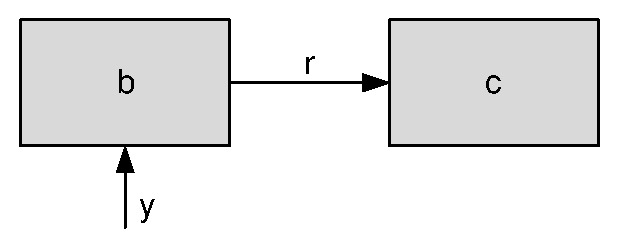
\includegraphics[width=.6\textwidth,clip, trim = 0cm 0cm 0cm 0cm]{2_Prinzip_Optimalsteuerung.eps} \\
  	\caption[Arbeitsweise der Optimalsteuerung]{Arbeitsweise der Optimalsteuerung \cite{foellingeroptimal}}
    \label{fig:arbeitspunktwechsel_optimalsteuerung_prinzip}
\end{figure} 
%
\begin{figure}[h]
\newcommand{\smallsize}{.85}
	\psfrag{1}[cr][cr][1.0]{$\bs x(t)$}
	\psfrag{2}[tc][tc][1.0]{$t$}
	\psfrag{u}[cr][cr][1.0]{$\bs u(t)$}
	\psfrag{m}[cr][cr][1.0]{$\bs u_{\min}$}
	\psfrag{z}[bc][bc][1.0]{$\bs x$}
	\psfrag{y}[cl][cl][1.0]{$\bs x_0$}
	\psfrag{b}[cc][cc][\smallsize]{\parbox[c]{7cm}{\begin{center}Optimal-\\ steuerung \end{center}}}
	\psfrag{c}[cc][cc][\smallsize]{\parbox[c]{7cm}{\begin{center}Strecke \end{center}}}
	\centering
  	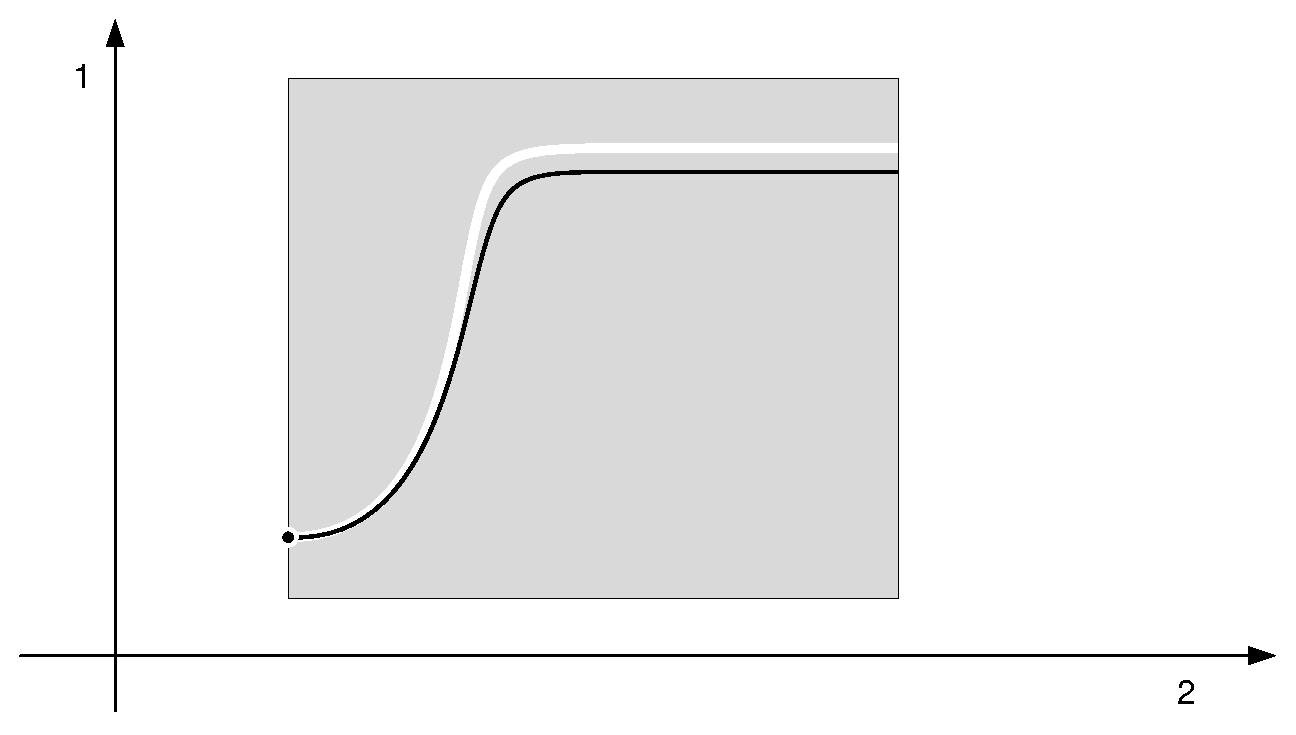
\includegraphics[width=.47\textwidth,clip, trim = 0cm 0cm 0cm 0cm]{2_arbeitspunktwechsel_optimalsteuerung.eps}
	\hspace{.5cm}
		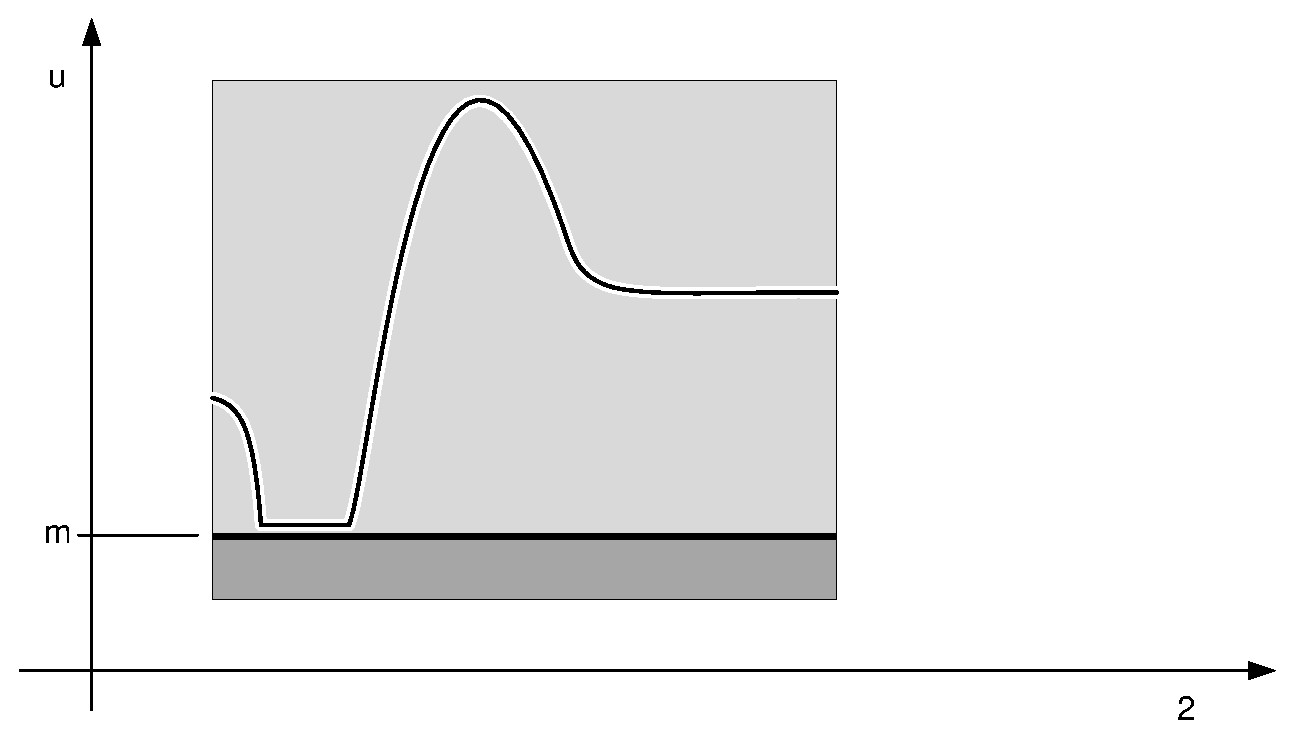
\includegraphics[width=.47\textwidth,clip, trim = 0cm 0cm 0cm 0cm]{2_arbeitspunktwechsel_optimalsteuerung_u.eps}
  	\caption[Signalverläufe der Optimalsteuerung]{Signalverläufe der Optimalsteuerung: Geplante Referenzverläufe des Zustands und der Stellgröße in Weiß, tatsächliche Verläufe in Schwarz; $\bs u_{\min}$ bezeichnet die (untere) Stellgrößensättigung; Aufgrund von Störungen kommt es zu einer merklichen Endabweichung zwischen geplanter und tatsächlicher Trajektorie.}
    \label{fig:arbeitspunktwechsel_optimalsteuerung}
\end{figure} 

\subsection{Optimale und Modellprädiktive Regelung} \label{sec:def_modellpraediktive_Regelung}
Das Fahrzeugumfeld ist stetig von nur schwer vorhersehbarem Wechsel geprägt, und damit ändert sich auch ständig das Optimierungsproblem. Ausgedehnte Fahreingriffe erfordern deshalb eine permanente Optimierung, die der neuen Umfeldinformation Rechnung trägt. 
Wird in der Regelungstechnik ein Optimalsteuerungsproblem ausgehend vom aktuellen Systemzustand $\bs x$ permanent gelöst  
%hierbei ausgehend vom aktuellen Systemzustand $x$ optimiert 
und das Ergebnis auf die Regelstrecke gegeben, so ergibt sich aufgrund der Rückführung ein geschlossener Regelkreis, s.\ Abb.\,\ref{fig:arbeitspunktwechsel_optimaleregelung_prinzip} und \ref{fig:arbeitspunktwechsel_optimaleregelung}. Anschaulich erfolgt die Stabilisierung des Systems über die Rückführung dadurch, dass der Systemzustand $\bs x$ die Wirkung der vorangegangen Störungen widerspiegelt \cite{foellingeroptimal}. Hierbei sind sich zufällige, impulsförmige Störungen vorzustellen, die das prädizierte Streckenverhalten nicht in Frage stellen. Im Unterschied zur Stabilisierung einer Trajektorie mittels nachgeschalteter Folgeregelung, die das System bei Impulsstörungen lediglich (mit hohen Stellgrößen!) auf die alte Referenz $\bs x_r(t)$ zurückführt, wird hier der aktuell gemessene Systemzustand optimal berücksichtigt. \\
Kann eine sehr schlanke, ggf. sogar analytische Lösung für das der Regelung zugrundeliegende Optimalsteuerungsproblem gefunden werden, so wird (tendenziell) von \emph{Optimaler Regelung}\index{Optimalregelung}  \cite{foellingeroptimal} gesprochen. Die Verwendung des Begriffs \emph{Modellprädiktive Regelung}\index{Modellprädiktiver Regelkreis} (\emph{model predictive control}, MPC) \cite{Findeisen2003} hingegen deutet auf ein für analytische Methoden zu schwieriges Optimalsteuerungsproblem hin, das in jedem Schritt numerisch auf einem verkürzten und sich zeitlich mitbewegenden\footnote{Es ist daher auch die Rede von \emph{receding horizon control}.} Optimierungshorizont\index{Optimierungshorizont} gelöst werden muss. 
Das trifft im Übrigen auch auf die Optimierung von Fahrmanövern zu, s.\ Abschn.\,\ref{sec:unendlichdim_opt}. Anhaltende, nicht vernachlässigbare Störungen und Modellfehler erfordern jedoch zusätzliche Maßnahmen, die genauer in Abschn.\,\ref{sec:unterlagerteRegelung} 
diskutiert werden.




\begin{figure}[h]
\newcommand{\smallsize}{.85}
	\psfrag{1}[cr][cr][1.0]{$\bs x(t)$}
	\psfrag{2}[tc][tc][1.0]{$t$}
	\psfrag{3}[cc][cc][.8]{$(\ldots)$}
	\psfrag{u}[cr][cr][1.0]{$\bs u(t)$}
	\psfrag{r}[bc][bc][1.0]{$\bs u^\ast$}
  \psfrag{m}[cr][cr][1.0]{$\bs u_{\min}$}
	\psfrag{z}[bc][bc][1.0]{$\bs x$}
	\psfrag{b}[cc][cc][\smallsize]{\parbox[c]{7cm}{\begin{center}Modellprädiktive\\ Regelung \end{center}}}
	\psfrag{c}[cc][cc][\smallsize]{\parbox[c]{7cm}{\begin{center}Strecke \end{center}}}
	\centering
			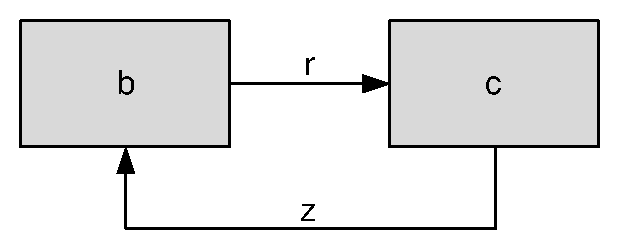
\includegraphics[width=.6\textwidth,clip, trim = 0cm 0cm 0cm 0cm]{2_Prinzip_Optimale_Regelung.eps}
  	\caption[Arbeitsweise der modellprädiktiven Regelung]{Arbeitsweise der modellprädiktiven Regelung, vgl.\ \cite{foellingeroptimal}}
    \label{fig:arbeitspunktwechsel_optimaleregelung_prinzip}
\end{figure}

\begin{figure}[h]
\newcommand{\smallsize}{.85}
	\psfrag{1}[cr][cr][1.0]{$\bs x(t)$}
	\psfrag{2}[tc][tc][1.0]{$t$}
	\psfrag{3}[cc][cc][.8]{$(\ldots)$}
	\psfrag{u}[cr][cr][1.0]{$\bs u(t)$}
	\psfrag{r}[bc][bc][1.0]{$\bs u$}
  \psfrag{m}[cr][cr][1.0]{$\bs u_{\min}$}
	\psfrag{z}[bc][bc][1.0]{$\bs x$}
	\psfrag{b}[cc][cc][\smallsize]{\parbox[c]{7cm}{\begin{center}Modellprädiktive\\ Regelung \end{center}}}
	\psfrag{c}[cc][cc][\smallsize]{\parbox[c]{7cm}{\begin{center}Strecke \end{center}}}
	\centering
  	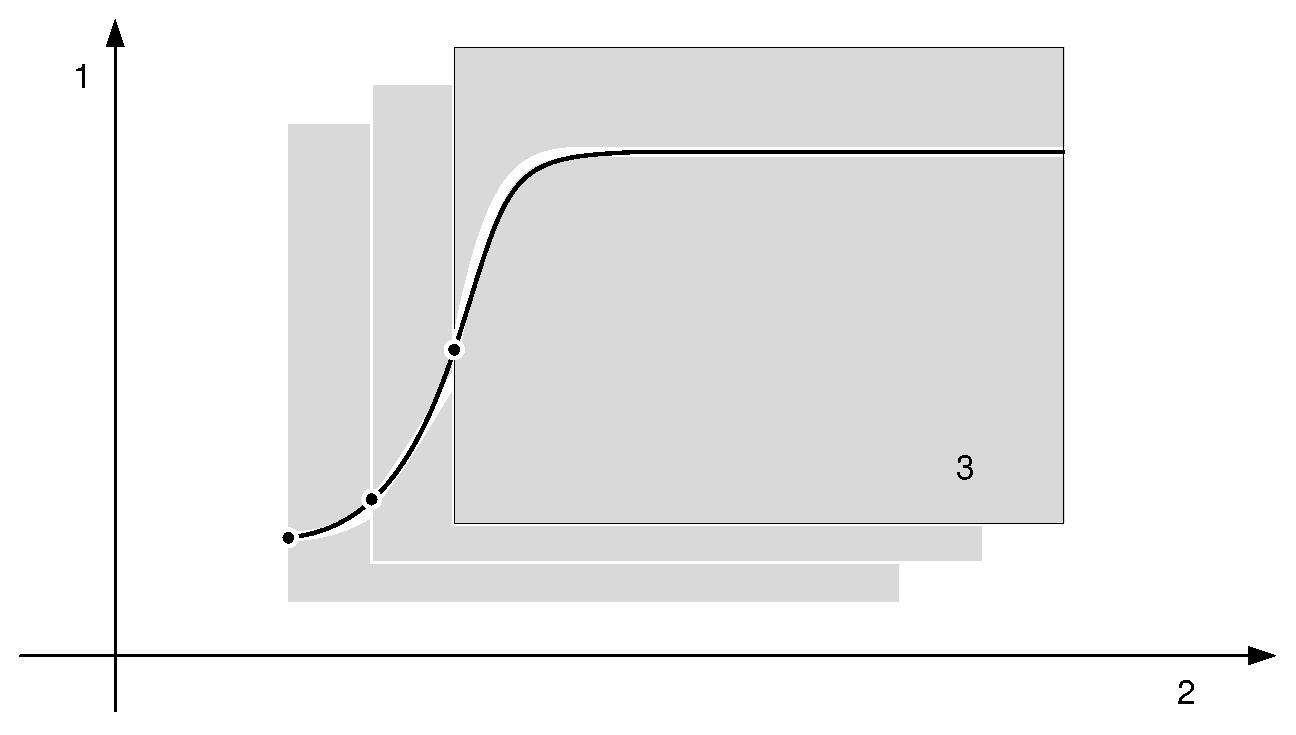
\includegraphics[width=.47\textwidth,clip, trim = 0cm 0cm 0cm 0cm]{2_arbeitspunktwechsel_optimaleregelung.eps}
	\hspace{.5cm}
		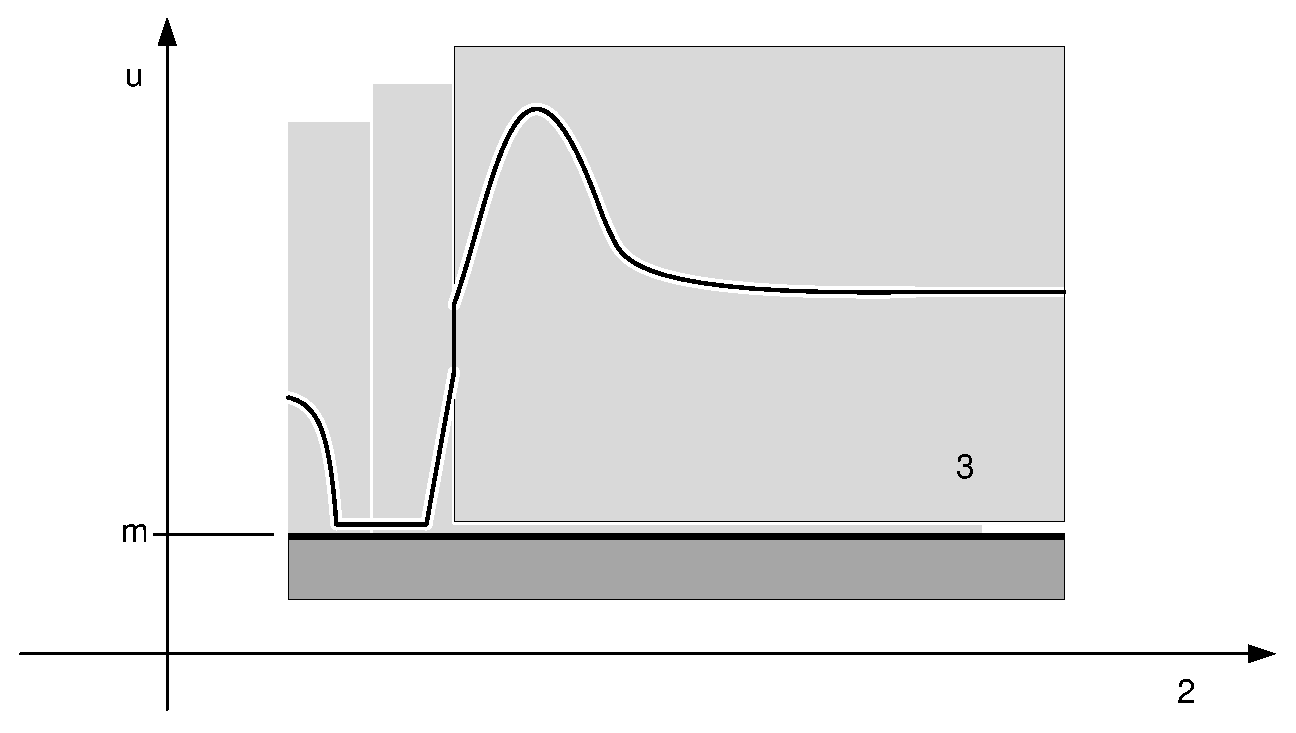
\includegraphics[width=.47\textwidth,clip, trim = 0cm 0cm 0cm 0cm]{2_arbeitspunktwechsel_optimaleregelung_u.eps}
  	\caption[Signalverläufe der modellprädiktiven Regelung]{Signalverläufe der modellprädiktiven Regelung, vgl.\ \cite{graichen2014SkriptOpt}: Auf einem sich zeitlich verschiebenden Horizont zyklisch geplante Referenzverläufe des Zustands und der Stellgröße in Weiß, tatsächliche Verläufe in Schwarz; $\bs u_{\min}$ bezeichnet die (untere) Stellgrößensättigung}
    \label{fig:arbeitspunktwechsel_optimaleregelung}
\end{figure}



\section{Aktorik\index{Aktorik} und Stellgrößen\index{Stellgröße}} \label{sec:aktuatorik}
Bei dem Entwurf und der Implementierung fahraktiver Sicherheits- und Komfortfunktionen ist ein tiefergehendes Verständnis über die technische Realisierung der Aktorikeingriffe von Lenkung, Bremse und Gas unverzichtbar. Insbesondere die mit der eingesetzten Hardware eng verkoppelten Möglichkeiten und Einschränkungen der Stellgrößenüberlagerung mit dem Fahrer sind von substantieller Bedeutung, da das Fahrerassistenzsystem, zumindest für kurze Zeit, mit dem Fahrer kooperiert. Darüber hinaus haben sich bestimmte Regelgrößen in den jeweiligen Aktoriksteuergeräten etabliert, die als vereinheitlichte Schnittstellen der Fahrerassistenz zur Verfügung stehen und somit die Stellgröße des überlagerten Regelkreises repräsentieren. Die Kenntnis über diese abstrahierten Schnittstellen und die mit ihren unterlagerten Reglern verbundenen Dynamiken erleichtern den Funktionsentwurf enorm, da sie "`böse Überraschungen"' verhindern. Darum wird im Folgenden der Aufbau und die Funktionsweise moderner Lenk-, Brems- und Antriebssysteme aus Fahrerassistenzsicht genauer beleuchtet.

\subsection{Lenkaktorik}
Im Pkw-Bereich kann in den letzten Jahren ein stetiger Übergang von hydraulischen  hin zu elektrischen Lenksystemen\index{elektrisches Lenksystem} (\emph{Electric Power Steering}, EPS) verzeichnet werden \cite{karch2007mechatronische}. Hierbei wird die herkömmliche Lenkunterstützung des druckbeaufschlagten Servoöls durch die Magnetfeldkraft des Elektromotors ersetzt. % (s.\ Abschn.\,\ref{sec:eps_Aufbau}). 
Das bringt den Vorteil mit sich, dass nur dann Energie benötigt wird, wenn der Fahrer auch lenkt und der Verbrauch erheblich gesenkt\footnote{Bei einem Mittelklassefahrzeug mit einem \unit[2,0]{l} Benzinmotor können Verbrauchseinsparungen von bis zu \unit[0,5]{l}\,/\unit[100]{km} erreicht werden \cite{pfeffer2013lenkungshandbuch}.} werden kann. \\ 
Gleichzeitig eröffnet die Ansteuerung des Elektromotors die Möglichkeit, dem Fahrer ein haptisches Feedback über das Lenkrad zu geben oder gar direkt die Lenkbewegung vorzugeben\footnote{Bei hydraulischen Lenksystemen erfordert das zusätzlich einen sog.\, Handmomentensteller, der auf hydraulische oder elektrische Weise das Fahrerhandmoment am Lenkrad nachahmt.}. Damit ist die EPS das wichtigste Stellglied der Fahrerassistenz zur Beeinflussung der Fahrzeugquerdynamik. % und wird im Folgenden genauer beleuchtet. 
\subsubsection{Systemkomponenten und -aufbau} \label{sec:eps_Aufbau}
Wie in Abb.\,\ref{fig:eps_funktionsweise} dargestellt, kann die Lenkunterstützung\index{Lenkunterstützung} des Elektromotors (M) je nach Gewichtung der Einflussfaktoren Kosten, Energieverbrauch, Akustik und Bauraum an der Lenksäule oder Zahnstange über ein Servogetriebe (G$_\text{M}$) eingeleitet werden. Über eine Drehmomentsensorik (S) wird das Fahrerhandmoment ($M_\text{Hand}$) gemessen und mittels der im Steuergerät befindlichen Software in das Motormoment ($M_\text{Motor}$) umgerechnet. Über die meist ebenfalls im Steuergerät integrierte Leistungselektronik erfolgt die entsprechende Ansteuerung des Motors \cite{pfeffer2013lenkungshandbuch}. Die hohe Flexibilität einer Steuergerätesoftware ermöglicht hierbei, den Unterstützungsgrad in Abhängigkeit des Fahrzustands nahezu beliebig zu variieren. \\
Beim Einsatz von variablen Übersetzungen im Zahnstangenlenkgetriebe (G$_\text{H}$) kann (abhängig vom Lenkwinkel) dem gesteigerten Lenkwinkelbedarf beim Parkieren und Rangieren Rechnung getragen werden. %Zur deutlichen Verbesserung des Gierverhaltens (Drehbewegung um die Hochachse, s.\ später Abschnitt \ref{sec:fahrzeugmodellierung}) auch bei mittleren Geschwindigkeiten kann, wenn auch mit hohen Kosten verbunden, ein Lenkwinkelüberlagerungssystem eingesetzt werden.
Eine noch höhere Flexibilität wird durch ein, wenn auch mit hohen Kosten verbundenes, Lenkwinkelüberlagerungssystem realisiert. Es sorgt durch einen weiteren Elektromotor in Kombination mit einem entweder vor %Audi
 oder unmittelbar nach dem Lenkmomentsensor installierten Winkelüberlagerungsgetriebe %BMW
für eine zusätzliche Verdrehung in der Lenksäule, sodass nahezu beliebige Übersetzungen realisiert werden können. \\
Die beschriebenen und weitgehend entkoppelten Einflussmöglichkeiten auf Lenkmoment und Lenkwinkel bzw.\ Spurstange und Radwinkel der Räder führen dazu, dass bereits heute Lenkfreiheitsgrade geschaffen werden, die einem Steer-by-Wire-System\index{steer-by-wire} \cite{odenthal2003ubertragung} sehr nahe kommen \cite{karch2007mechatronische}. 

\begin{figure}[ht]
	\psfrag{M}[cc][cc][1.0]{M}
	\psfrag{G}[cc][cc][1.0]{G$_\text{M}$}
	\psfrag{I}[cc][cc][1.0]{G$_\text{H}$}
	\psfrag{S}[cc][cc][1.0]{S}
	\psfrag{3}[tl][tl]{$M_\text{Motor}$}
	\psfrag{4}[cl][cl]{$M_\text{Hand}$}
	\psfrag{5}[cb][cb]{$F_z$}
	\psfrag{6}[tl][tl]{$M_\text{Motor}$}
\centering
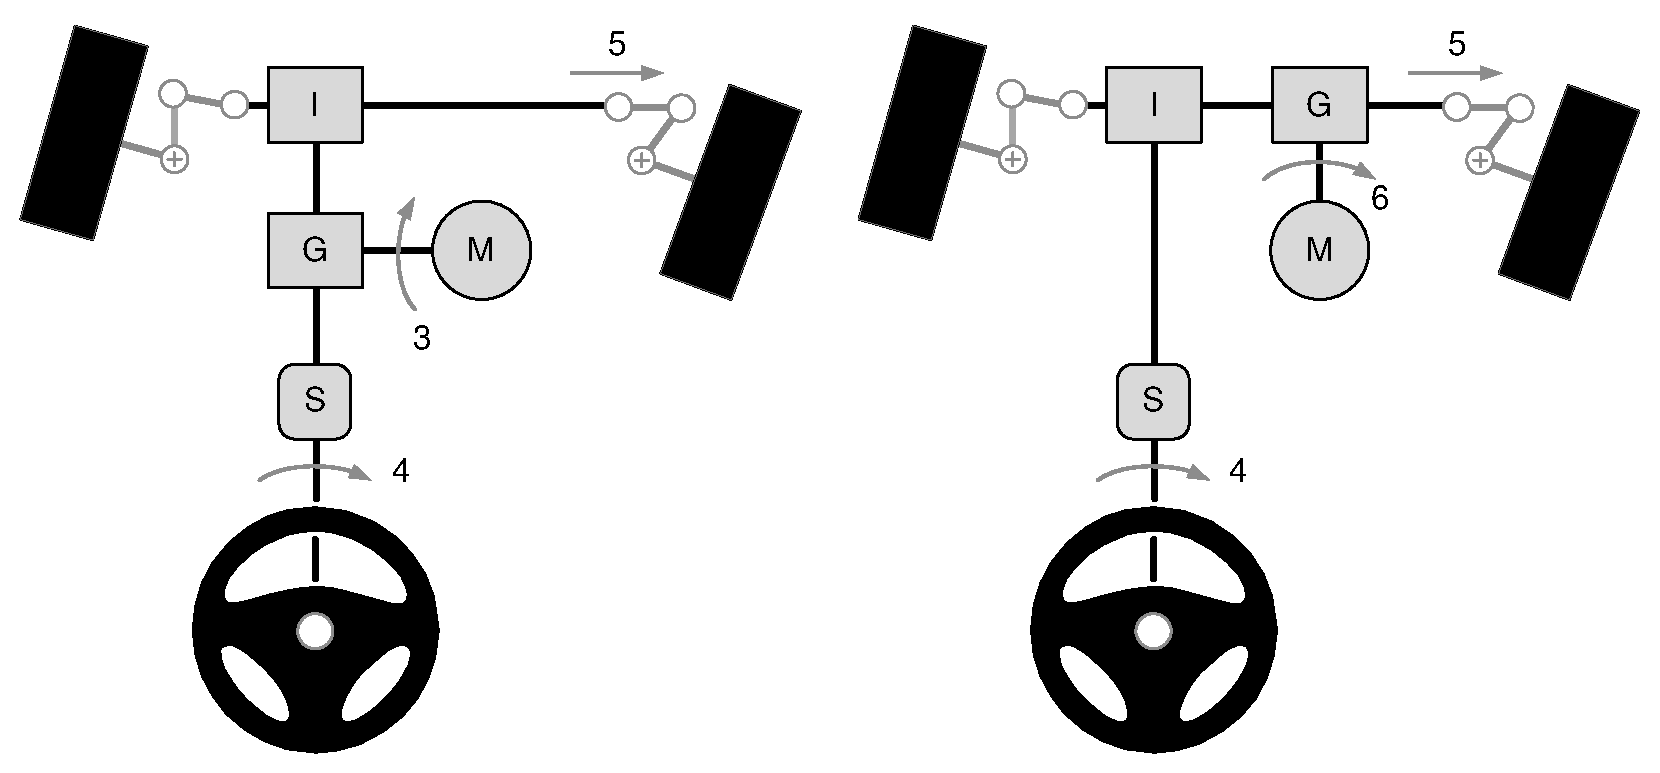
\includegraphics[width=1.0\textwidth,clip, trim = 0cm 0cm 0cm 0cm]{2_EPS_Komponenten.eps}
 \caption[Lenksäulen-basiertes und Zahnstangen-basiertes EPS-System]{Lenksäulen-basiertes (links) und Zahnstangen-basiertes EPS-System (rechts) mit Motor (M), Handmomentsensor (S), Servogetriebe (G$_\text{M}$) und Zahnstangenlenkgetriebe (G$_\text{H}$), vgl.\ \cite{pfeffer2013lenkungshandbuch}}
 \label{fig:eps_funktionsweise}
\end{figure} 

\subsubsection{Funktionsweise} \label{sec:eps_funktionsweise}
%\textbf{Klassisches Regelungskonzept} \\
Das dem herkömmlichen Hydrauliklenksystem nachempfundene Regelungsprinzip zur Bestimmung des elektrischen Servomoments beruht auf der progressiven Verstärkung des Handmoments. Wie in Abb.\,\ref{fig:eps_grundfunktion} dargestellt, wird das gemessene Handmoment entsprechend einem geschwindigkeitsabhängigen Kennfeld $K(v)$ überproportional verstärkt und damit über das Servogetriebe das Lenksystem beaufschlagt. Hierdurch wird erreicht, dass sich (unter Vernachlässigung von Reibungseffekten) die stationäre Zahnstangenkraft $F_z$, Abb.\,\ref{fig:eps_funktionsweise}, zu
\begin{align}
\label{equ:eps_f_z_0}
	F_z &= i_\text{Hand} M_\text{Hand} + i_\text{Motor} M_\text{Motor} \\
	\label{equ:eps_f_z}
	&= i_\text{Hand} M_\text{Hand} + i_\text{Motor} K(v;M_\text{Hand}) 
\end{align}
ergibt, wobei $i_\text{Hand}$ und $i_\text{Motor}$ die jeweiligen Gesamtübersetzungen der Momente auf die Zahnstangenkraft darstellen. \\
Die Höhe des Unterstützungsgrads aus dem Kennfeld hat einen entscheidenden Einfluss auf das Lenkgefühl. So wird durch dessen Geschwindigkeitsadaption hin zu einer reduzierten Servounterstützung bei höheren Geschwindigkeiten erreicht, dass der Fahrer vermehrt die Zahnstangenkraft an der Lenkung verspürt und damit eine differenzierte Rückmeldung von der Fahrbahn erhält. Beim Parkieren und Rangieren hingegen, wo die Zahnstangenkräfte am höchsten ausfallen, kann auf diese Informationsquelle verzichtet werden, sodass zugunsten des Komforts der Unterstützungsgrad deutlich erhöht wird \cite{pfeffer2013lenkungshandbuch}.

\begin{figure}[ht]
\newcommand{\smallsize}{.8}
	\psfrag{1}[cc][cc][1.0]{Lenksystem}
	\psfrag{3}[cb][cb]{$M_\text{Motor}$}
	\psfrag{4}[cb][cb]{$M_\text{Hand}$}
	\psfrag{t}[cc][cc][\smallsize]{{\parbox[c]{7cm}{\begin{center} Reibungskompensation \\ Trägheitskompensation \\ Dämpfung \end{center}}}}
	\psfrag{5}[cc][cc][1.0]{$K$}
	\psfrag{6}[cb][cb][1.0]{$M_{\text{Hand},d}\!=\!0$}
\centering
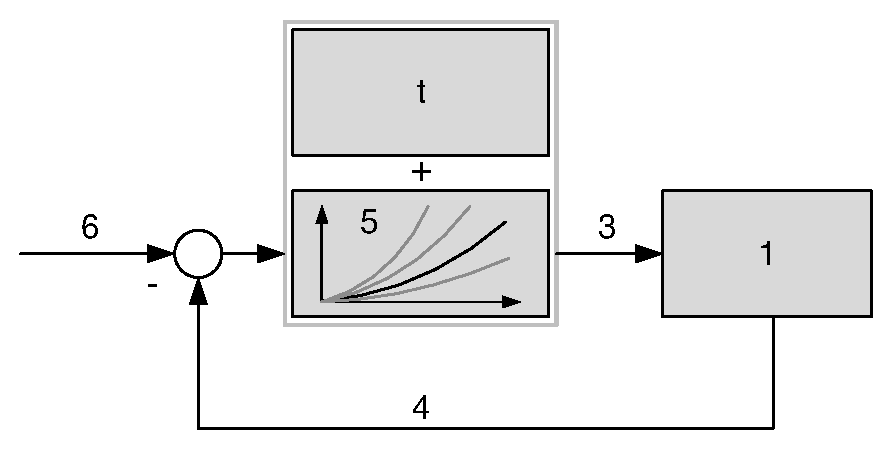
\includegraphics[width=.85\textwidth,clip, trim = 0cm 0cm 0cm 0cm]{2_EPS_Grundfunktion.eps}
 \caption[Herkömmliches Regelungsprinzip der elektrischen Servolenkung]{Herkömmliches Regelungsprinzip der elektrischen Servolenkung, vgl.\ \cite{pfeffer2013lenkungshandbuch}}
 \label{fig:eps_grundfunktion}
\end{figure} 

Eine weitere Verbesserung des Lenkgefühls wird über eine sog.\ Reibungs- und Trägheitskompensation erzielt, wobei das Ziel ist, die inhärenten mechanischen Eigenschaften des Lenksystems so weit durch das Motormoment zu kompensieren, dass auch im instationären, reibungsbehafteten Fall Gleichung~\eqref{equ:eps_f_z} näherungsweise gilt. Da hierdurch das Lenksystem sehr empfindlich auf Anregungen der Straße und des Fahrers reagiert, muss gleichzeitig  die Lenkbewegung über das Motormoment gedämpft werden, s.\ Abb.\,\ref{fig:eps_grundfunktion}, was regelungstechnisches Know-how der Lenkungshersteller erfordert. \\
Formal ergibt sich hierdurch der in Abb.\,\ref{fig:eps_grundfunktion} dargestellte Regelkreis\footnote{Die Darstellungsweise der vorliegenden Arbeit beruht durchgängig auf einem Regelfehler, welcher als Differenz zwischen Soll- und Istwert definiert ist. Das hat zur Folge, dass sich im Standardregelkreis die Vorzeichen des Komparators (dargestellt als Kreis in Abb.\,\ref{fig:eps_grundfunktion}) umdrehen.}, dessen (bleibende) Regelabweichung von Null das Handmoment darstellt \cite{pfeffer2013lenkungshandbuch}. Das Lenkgefühl ist dadurch unmittelbar mit der Regelung verbunden. Darüber hinaus besteht im regelungstechnischen Sinne keine direkte Möglichkeit für Fahrerassistenzfunktionen, zusätzliche Handmomente aufzubringen, %\footnote{Als Behelf kann jedoch das gemessene Handmoment um das Zusatzhandmoment korrigiert werden.}, 
sodass neue Regelungskonzepte entworfen wurden, die als Regelgröße eine intern berechnete Handmomentreferenz, das "`Soll-Lenkgefühl"', heranziehen. Aufgrund ihrer prognostizierten hohen Bedeutung werden nun auch sie kurz erläutert.
%


Während sich das herkömmliche Regelungsprinzip stark an der hydraulischen Arbeitsweise einer Servolenkung orientiert, löst sich das neue Konzept davon völlig. Es begreift vielmehr die EPS mit ihren gesteigerten Freiheitsgraden als ganzheitliches Mechatroniksystem, dessen primäres Regelziel die Realisierung eines Sollhandmoments $M_\text{{Hand},d}$ ist \cite{pfeffer2013lenkungshandbuch}, s.\ Abb.\,\ref{fig:eps_Momentregelung}. Die Kompensation der Reibung und Trägheit, welche ja Teil der Regelstrecke sind, erfolgt hierbei automatisch. \\
Für die Handmomentregelung\index{Handmomentregelung} selbst eignet sich prinzipiell die gesamte Bandbreite an Regelungsverfahren. Die Sollmomentberechnung wiederum ist aktueller Forschungsgegenstand, s.\ beispielsweise \cite{patentDE102010030986}, wobei dafür das idealisierte Kräftegleichgewicht \eqref{equ:eps_f_z_0} an der Zahnstange ein guter Anhaltspunkt ist. Aus Kostengründen steht in der Praxis kein Messsignal für die Zahnstangenkraft $F_z$ zur Verfügung, sodass es über Fahrzeugmodelle aus dem aktuellen Fahrzustand geschätzt werden muss. Letztendlich entscheidet deren Güte über die Qualität der Reifenkraftrückmeldung an den Fahrer.

\begin{figure}[ht]
	\psfrag{1}[cc][cc][1.0]{Lenksystem}
	\psfrag{3}[cb][cb]{$M_\text{Motor}$}
	\psfrag{4}[cb][cb]{$M_\text{Hand}$}
	\psfrag{5}[cc][cc]{{\parbox[c]{7cm}{\begin{center} Fahrer- \\ assistenz \end{center}}}}
	\psfrag{6}[cb][cb]{$M_{\text{Hand},d}$}
	\psfrag{7}[cc][cc]{{\parbox[c]{7cm}{\begin{center} Sollwert- \\ generierung \end{center}}}}
	\psfrag{8}[cc][c]{{\parbox[c]{7cm}{\begin{center} Handmoment- \\ regelung \end{center}}}}
	\psfrag{9}[cb][cb]{$M_\text{Hand,FAS}$}
\centering
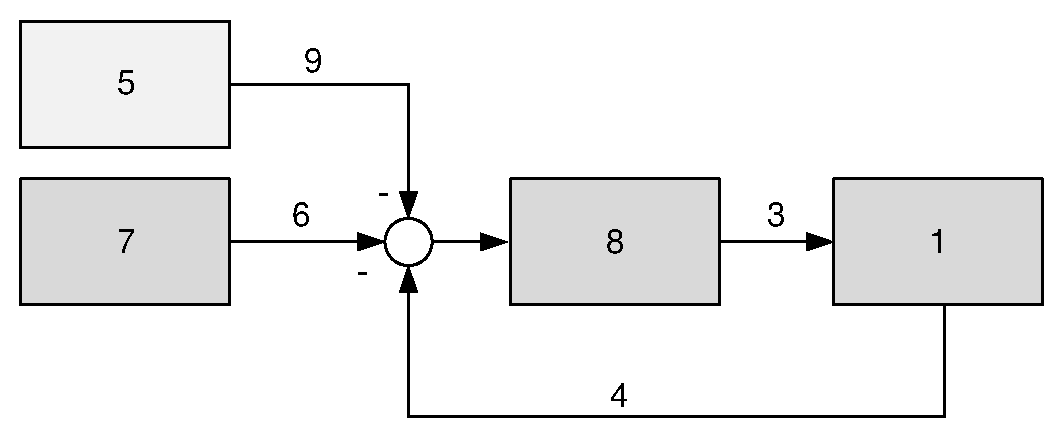
\includegraphics[width=1.\textwidth,clip, trim = 0cm 0cm 0cm 0cm]{2_EPS_Momentenregelung.eps}
 \caption[Moderne Handmomentregelung der elektrischen Servolenkung]{Moderne Handmomentregelung der elektrischen Servolenkung, vgl.\ \cite{pfeffer2013lenkungshandbuch}}
 \label{fig:eps_Momentregelung}
\end{figure} 

Für die Fahrerassistenz ist aber ein ganz anderer Punkt entscheidend. Durch die gegenüber des herkömmlichen Regelungsprinzips geänderte Struktur ist es nun möglich,  ein zusätzliches Fahrerhandmoment $M_\text{Hand,FAS}$ (entkoppelt von der Auslegung der Handmomentregelung) vorzugeben, s.\ Abb.\,\ref{fig:eps_Momentregelung}, das sich direkt als Offset zur gewohnten Lenkhaptik dem Fahrer bemerkbar macht und eine Vielzahl von Assistenzfunktionen wie die Spurhalteunterstützung ermöglicht.

Im Unterschied zu Assistenzsystemen mit Lenkunterstützungsfunktion, bei denen der Fahrer die Hände am Lenkrad behält (es wird auch von \emph{shared guidance} \cite{Brandt2008} gesprochen), stellt sich bei den automatisierten Lenkfunktionen, wie dem automatischen Einparken, das Reglerentwurfsziel für die EPS anders dar. Anstelle der Umsetzung einer Lenkhaptik tritt eine genaue Winkelregelung\index{Winkelregelung}, sodass sich die Reifen des Fahrzeugs entsprechend der umzusetzenden Assistenzfunktion bewegen. Für Parksysteme hat sich als Schnittstelle ein Lenkradwinkel-Referenzsignal~$\delta_{h,d}$ etabliert\footnote{Alternativ eignet sich auch die Zahnstangenposition, der sog.\ Zahnstangenhub.}, welches über die Lenkkinematik aus dem angestrebten Lenkwinkel~$\delta_{d}$ an den Reifen zu berechnen ist. Anschließend wird es der EPS über den Fahrzeug-Bus übermittelt und dort eingeregelt. 
%Grundvoraussetzung hierfür eine bekannte Lenkwinkelkinematik, sodass der angestrebte Lenkwinkel~$\delta_{h,d}$ an den Reifen zuvor in den Lenkradwinkel~$\delta_{h,d}$ umgerechnet werden kann.
Das dabei zugrundeliegende Verfahren, s.\ Abb.\,\ref{fig:eps_kaskade}, bedient sich der vor allem in der Antriebstechnik verbreiteten Kaskadenregelung\index{Kaskadenregelung}, s.\ beispielsweise \cite{graf2003neue} und auch \abschn{sec:unterlagerteRegelung}. Der Entwurf erfolgt typischerweise von den inneren, d.h. stellgrößennahen, hin zu den äußeren Regelkreisen, die sukzessive weitere Teile der Strecke mit einbeziehen, s.\ Abb.\,\ref{fig:eps_kaskade}. Hierbei liefert der Ausgang des jeweils überlagerten Reglers das Referenzsignal des unterlagerten. Im konkreten Fall der Lenkradwinkelregelung wird ganz innen eine auf den in der EPS verbauten Elektromotor abgestimmte Momentregelung eingesetzt. Die darüber liegenden Regelkreise stabilisieren, i.\,Allg.\ als modifizierte PID-Regelungen, die Lenkrate $\omega$ und schließlich den Lenkradwinkel $\delta_h$, wozu beide als Messsignal vorliegen müssen. % (s.\ Abschn.\,\ref{sec:sensoren}).
Aufgrund der nach innen schneller werdenden Dynamik ist es ratsam, zumindest die beiden inneren Regelkreise auf dem Steuergerät der EPS umzusetzen, da ansonsten die latenzbehaftete Übertragung von und zu der EPS zu einer erheblichen Minderung der erreichbaren Regelqualität führt. \\
%
Eine Lenkwinkelregelung, wenn auch mit geringer Dynamik und reduzierter Winkelamplitude von unter fünf Grad, kommt auch bei der elektromechanischen Hinterachslenkung\index{Hinterachslenkung} zum Einsatz \cite{pfeffer2013lenkungshandbuch}. Analog zur Lenkkinematik der Vorderachse werden die Räder der Hinterachse durch einen zusätzlichen elektrischen Aktor mit entsprechendem Getriebe gleichsinnig eingelenkt; eine mechanische Kopplung zum Lenkrad existiert jedoch nicht. %Für den konkreten Einsatzzweck eines solchen Lenksystems wird auf Abschn.\,\ref{sec:Hinterachslenkung} verwiesen.


\begin{figure}[h]
\newcommand{\smallsize}{.75}
	\psfrag{a}[cb][cb][1.0]{$\omega$}
	\psfrag{b}[cb][cb][1.0]{$\delta_h$}
	\psfrag{c}[cb][cb][1.0]{$\delta_{h,d}$}
	\psfrag{d}[cb][cb][1.0]{$\omega_{d}$}
	\psfrag{e}[cb][cb][1.0]{$M_d$}
	\psfrag{1}[cc][cc][\smallsize]{{\parbox[c]{7cm}{\begin{center} Motor- \\ dynamik \end{center}}}}
		\psfrag{3}[cc][cc][\smallsize]{{\parbox[c]{7cm}{\begin{center} Moment- \\ regelung \end{center}}}}
		\psfrag{4}[cc][cc][\smallsize]{{\parbox[c]{7cm}{\begin{center} Lenkraten- \\ regelung \end{center}}}}
				\psfrag{5}[cc][cc][\smallsize]{{\parbox[c]{7cm}{\begin{center} Lenkwinkel- \\ regelung \end{center}}}}
	\psfrag{2}[cc][cc][1.0]{$\int$}
\centering
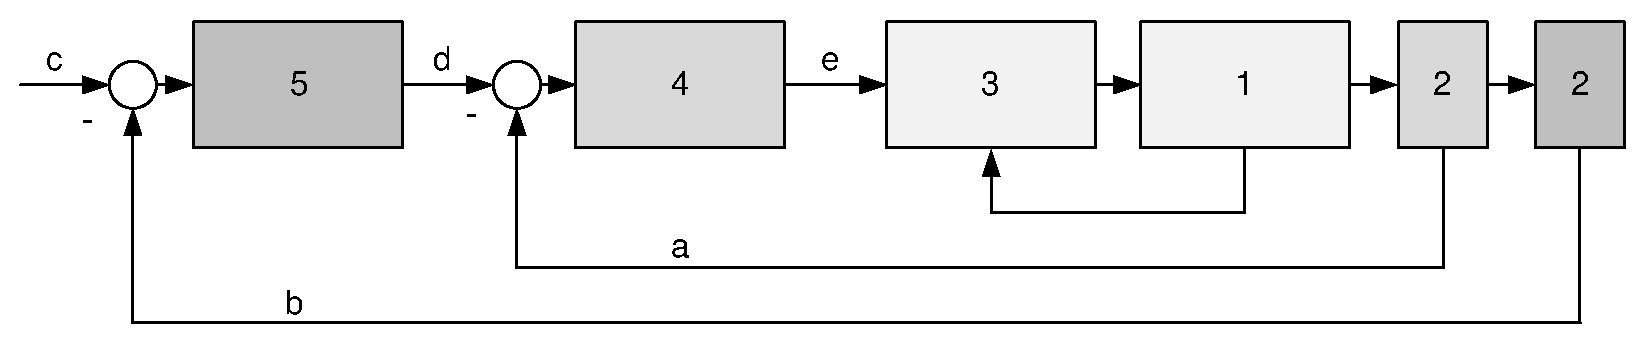
\includegraphics[width=1.\textwidth,clip, trim = 0cm 0cm 0cm 0cm]{2_EPS_Kaskade.eps}
 \caption[Kaskadierter Lenkwinkelregelkreis]{Kaskadierter Lenkwinkelregelkreis mit außen liegender Winkelstabilisierung sowie unterlagerter Lenkraten- und Motormomentregelung, vgl.\ \zB \cite{graf2003neue}}
 \label{fig:eps_kaskade}
\end{figure} 

\subsection{Bremsaktorik\index{Bremsaktorik}}
% Elektromechanische Bremse (EMB) -> Zukunftsmusik
% Elektrohydraulische Bremse (EHB)
%  --> Wichtig
% 1) Mit Druckspeicher und Druckmodulator -> Energie wird hydraulisch gespeichert und bei Bedarf in Bremsdruck umgewandelt
% 2) Mit Elektrohydraulischem Wandler -> Bremsdruck wird bei Bedarf direkt generiert --> TRW und Conti
%
% Conti: Kopplung zwischen Simulator und Notbetrieb wird hydraulisch realisiert (Ventile)
% TRW-FBS: Nutzt das Volumen im elektrischen Plunger auch für den Notbetrieb
%
Eine ganze Reihe von bremsaktiven Sicherheits- und Komfortfunktionen sowie der zunehmende Bedarf an rekuperativem Verzögern bei Elektro- und Hybridfahrzeugen führten zur Entwicklung von elektro-hydraulischen Bremsen\index{elektro-hydraulische Bremse} (EHB) \cite{breuer20012bremsenhandbuch}. Sie basieren in weiten Bereichen auf konventionellen hydraulischen Radbremsen, setzen jedoch eine energetische Bremspedalentkopplung um, sodass die Bremskraft des Fahrers beliebig mit externen Bremsmomenten, etwa zur automatischen Notbremsung, überlagert werden kann. Da die EHB grundsätzlich das Potential besitzt, analog zur EPS, bestehende Systeme langfristig komplett abzulösen, wird im Folgenden ihre Funktionsweise ausgeführt.

\subsubsection{Systemkomponenten und -aufbau}
Anders als bei herkömmlichen Bremssystemen, bei denen das Pedalgefühl durch den eigentlichen Bremsmechanismus entsteht, betätigt bei der EHB
der Fahrer lediglich einen gedämpften Federmechanismus, den sog.\ \emph{Simulator}. Über daran angeschlossene Druck- und Wegsensoren wird dabei die ermittelte Wunschverzögerung des Fahrers abgeleitet. Sie kann dann, und darin liegt der große Vorteil, beliebig mit externen Signalen überlagert werden, bevor die entsprechende Sollverzögerung über brake-by-wire\index{brake-by-wire} eingeregelt wird. Bremst der Fahrer, so kann das System \zB eigenständig entscheiden, wie die angeforderte Sollverzögerung idealerweise auf Rekuperations- und Bremsmoment aufzuteilen ist.\\
Im Folgenden wird die EHB basierend auf einem leistungsstarken elektrischen Zentraldruckaktor beschrieben, der dank eines linear angetriebenen Kolbenverdrängers einen latenzarmen und pulsationsfreien Druckaufbau gewährleistet; beides Voraussetzung für eine hohe Regelgüte der überlagerten Sicherheits- und Komfortfunktionen.

\begin{figure}[h]
\newcommand{\smallsize}{.75}
	\psfrag{1}[cc][cc][1.0]{V$\!_{1o}$}
	\psfrag{A}[cc][cc][1.0]{V$\!_{1i}$}
	\psfrag{W}[cc][cc][1.0]{V$\!_{1c}$}
	\psfrag{2}[cc][cc][1.0]{V$\!_{2o}$}
	\psfrag{B}[cc][cc][1.0]{V$\!_{2i}$}
	\psfrag{X}[cc][cc][1.0]{V$\!_{2c}$}
	\psfrag{3}[cc][cc][1.0]{V$\!_{3o}$}
	\psfrag{C}[cc][cc][1.0]{V$\!_{3i}$}
	\psfrag{Y}[cc][cc][1.0]{V$\!_{3c}$}
	\psfrag{4}[cc][cc][1.0]{V$\!_{4o}$}
	\psfrag{D}[cc][cc][1.0]{V$\!_{4i}$}
	\psfrag{Z}[cc][cc][1.0]{V$\!_{4c}$}
	\psfrag{M}[cc][cc][1.0]{M}
	\psfrag{S}[cc][cc][1.0]{S}
	\psfrag{R}[cc][cc][1.0]{R}
	\psfrag{K}[cc][cc][1.0]{V$\!_{s\,\,}$}
	\psfrag{s}[cc][cc][1.0]{S$_{s}$}
	\psfrag{r}[cc][cc][1.0]{S$_{p1}$}
	\psfrag{n}[cc][cc][1.0]{S$_{p2}$}
	\psfrag{m}[cc][cc][1.0]{S$_{s}$}
	\psfrag{T}[cb][cb][1.0]{THZ}
\centering
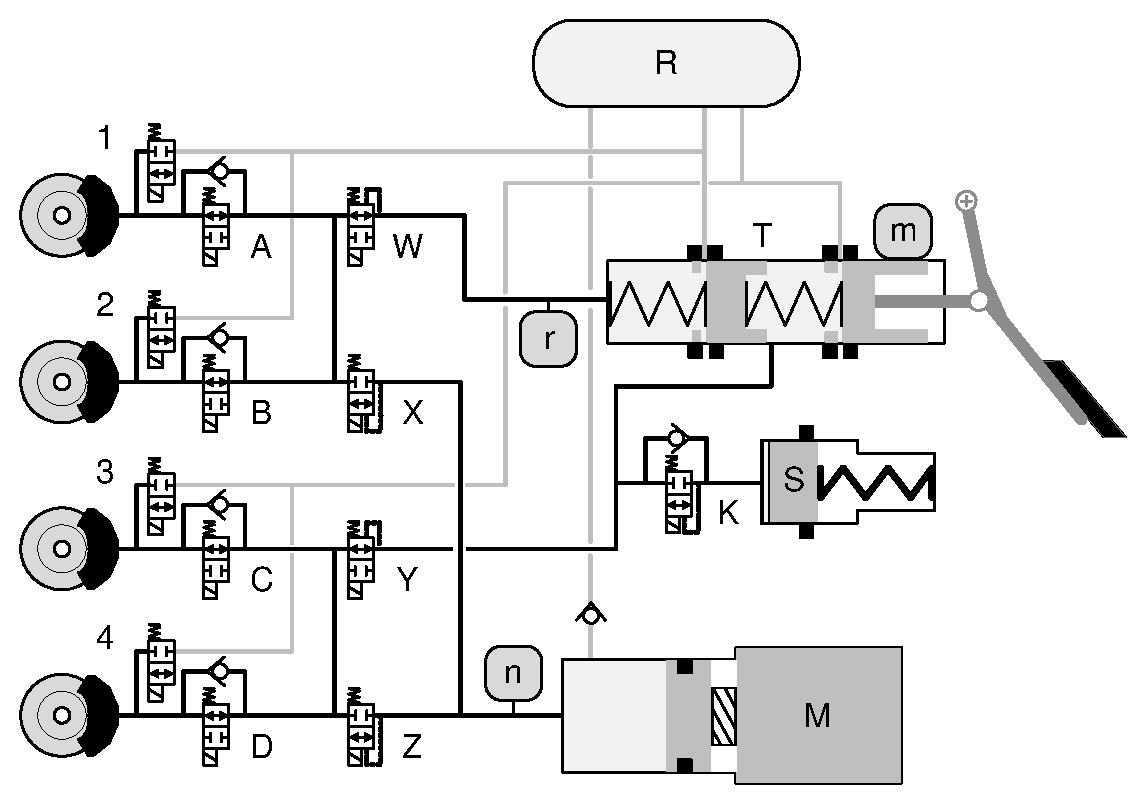
\includegraphics[width=1.\textwidth,clip, trim = 0cm 0cm 0cm 0cm]{2_EHB_Komponenten.eps}
 \caption[Elektrohydraulisches Bremssystem]{Elektrohydraulisches Bremssystem (EHB) mit Tandemhauptbremszylinders (THZ), elektrischem Zentraldruckaktor (M), Simulator (S), Ventilen (V$_{ij}$), Weg- (S$_{s}$) und Drucksensoren (S$_{pi}$) sowie Bremsflüssigkeitsreservoir (R); vgl.\cite{breuer20012bremsenhandbuch}}
 \label{fig:ehb_aufbau}
\end{figure} 


\subsubsection{Funktionsweise} \label{sec:ehb_funktionsweise}
Die Arbeitsweise der EHB wird aus Abb.\,\ref{fig:ehb_aufbau} ersichtlich, worin alle Ventile im stromlosen Zustand abgebildet sind. Den nehmen sie bei einem elektrischen Systemausfall ein, sodass die mechanische Rückfallebene wirksam wird. Betätigt der Fahrer dann das Bremspedal, so wird aus den beiden\footnote{Aus Redundanzgründen werden Bremssysteme immer in zwei getrennte Bremskreise aufgeteilt.} Kammern des Tandemhauptbremszylinders THZ durch die geöffneten Trennventile V$\!_{1c}$ und V$\!_{3c}$ und ABS-Einlassventile V$\!_{1i}$ -- V$_{4i}$ Öl zu den Bremsen gefördert, das infolge der geschlossenen ABS-Auslassventile V$\!_{1o}$ -- V$\!_{4o}$  und Trennventile V$\!_{2c}$ und V$\!_{4c}$ den Druck $p$ aufbaut. Aufgrund des geschlossenen Simulatorventils V$\!_s$ ist hierbei der Simulator S abgekoppelt, sodass die vom Fahrer auf das Pedal übertragene Betätigungsenergie ausschließlich dem behelfsmäßigen Verzögern der Räder dient. \\
Im Normalbetrieb sind V$\!_{1c}$ und V$\!_{3c}$ geschlossen sowie V$\!_s$, V$\!_{2c}$ und V$\!_{4c}$ geöffnet. Hierdurch gelangt das vom Fahrer verdrängte Volumen %des HBZ-Primärkreises 
ausschließlich in den Simulator, der das angestrebte Pedalgefühl realisiert. Über den Drucksensor S$_{p1}$ und den Wegsensor S$_s$ berechnet sich das Wunschbremsmoment des Fahrers und wird mit ggf.\ vorhandenen externen Vorgaben überlagert. Der abgeleitete Zielbremsdruck wird schließlich über den Zentraldruckaktor (M) unter Rückführung des Messwerts des Drucksensors S$_{p2}$ durch die offenen Ventile V$\!_{2c}$ und V$\!_{4c}$ in den beiden Bremskreisen eingeregelt. 
Über den sog.\ $C^\ast$-Wert\footnote{Verhältnis der in den Reibflächen entstehenden Umfangskraft zur aufgebrachten Spannkraft} der Bremse, die Bremskolbenfläche $A$ und den effektiven Bremsradius $r_\text{eff}$ berechnet sich das Bremsmoment zu
\begin{align*}
	M_B = C^\ast \cdot r_\text{eff}\cdot A \cdot p\;,
\end{align*}
worüber durch Auflösen der Sollbremsdruck an den Rädern bestimmt werden kann, der dann vom an den Fahrzeug-Bus angeschlossenen Bremssteuergerät eingeregelt wird.
Durch die vom Fahrer vollkommen entkoppelte Vorgabe von Bremsmomenten ist aus Fahrerassistenzsicht die mit brake-by-wire verknüpfte Flexibilität im vollen Umfang gegeben, 
ohne dass auf eine mechanische Rückfallebene verzichtet werden muss. \\
Zur radselektiven Bremsung, die für das ABS und ESP von so großer Bedeutung ist, können die Ventile V$\!_{1i}$ -- V$_{4i}$ und V$\!_{1o}$ -- V$_{4o}$ einzeln angesteuert werden, sodass der in den Bremsbacken anliegende Druck aufgebaut, gehalten oder abgelassen werden kann.

\subsection{Antrieb\index{Antrieb}} \label{sec:motorregelung}
% http://www.patent-de.com/20071122/DE19812485B4.html
% http://www.patent-de.com/19941110/DE69007902T2.html
Im Unterschied zu den Lenk- und Bremssystemen ist beim Verbrennungsmotor schon längst eine By-wire-Ansteuerung etabliert, das sog.\ \emph{E-Gas}\index{E-Gas} \cite{isermann2010mechatronische}. Das Gaspedal des Fahrers ist dabei nicht mehr mechanisch an den Motor gekoppelt, sondern besitzt einen Sensor zur Bestimmung des Pedalhubs, entsprechend dessen Messwert die Öffnung der elektronischen Drosselklappe eingestellt wird. Aufgrund des anhaltend hohen Stellenwerts des Verbrennungsmotors im Individualverkehr werden die für die Fahrerassistenz relevanten Aspekte der Motorregelung und der Getriebesteuerung nun nacheinander beleuchtet.  

\begin{figure}[h]
	\psfrag{Z}[cc][cc][1.0]{Z}
	\psfrag{E}[cc][cc][1.0]{E}
	\psfrag{n}[cc][cc][1.0]{S$_n$}
	\psfrag{D}[cc][cc][1.0]{D}
	\psfrag{p}[cc][cc][1.0]{S$_w$}
\centering
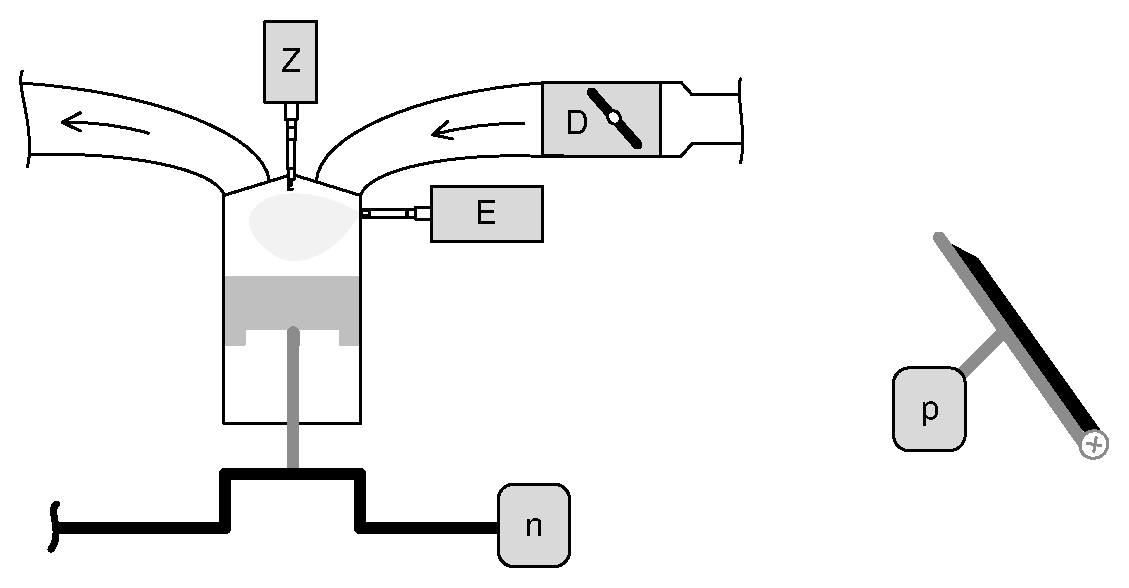
\includegraphics[width=.7\textwidth,clip, trim = 0cm 0cm 0cm 0cm]{2_Benzinmotor_Komponenten.eps}
 \caption[Vereinfachte Darstellung eines Saugeinspritzer-Motors]{Vereinfachte Darstellung eines Saugeinspritzer-Motors mit Pedalwertgeber (S$_w$), Motordrehzahl-Sensor (S$_n$), Drosselklappe (D), Einspritzventil (E) und Zündspule (Z); vgl. \cite{isermann2010mechatronische}}
 \label{fig:motor_aufbau}
\end{figure} 


\subsubsection{Funktionsweise der Motorregelung}
Bei einer modernen sog.\ \emph{drehmomentorientierten Regelung}\index{drehmomentorientierte Regelung} \cite{patentDE19812485B4, patentDE69007902T2} wird nicht einfach der ausgelesene Fahrerpedalwert $\alpha_d$ entsprechend eines simplen Kennfelds auf die Drosselklappenstellung $\alpha_e$ übertragen und damit eine mechanische Verbindung nachgeahmt. Vielmehr werden, analog zur Bremsmomentregelung in Abschn.\,\ref{sec:ehb_funktionsweise}, die Freiheitsgrade eines elektronischen Steuergeräts dazu genutzt, aus dem Fahrerpedalwert (erfasst durch S$_w$, s.\ Abb.\,\ref{fig:motor_aufbau}) zunächst ein Wunschantriebsmoment $M_d$ abzuleiten\footnote{Je nach Fahrmodus (\emph{Sport}, \emph{Eco} etc.) wird zwischen unterschiedlichen Pedalcharakteristiken umgeschalten.}, s.\ \abb{fig:motor_funktionsweise}. Nach Belieben kann es mit externen, \zB von der  Fahrerassistenz herrührenden Signalen $M_\text{FAS}$ zu einem Sollmoment überlagert werden. % und unter Berücksichtigung verschiedener Messgrößen (z.B.\ hauptsächlich die Drehzahl gemessen durch S$_n$) %über die Drosselklappe (D)  eingeregelt werden. 

\begin{figure}[h]
\newcommand{\smallsize}{.75}
	\psfrag{a}[cb][cb][1.0]{$\alpha_d$}
	\psfrag{b}[cr][cr][1.0]{$n$}
	\psfrag{c}[cb][cb][1.0]{$M_d$}
	\psfrag{d}[cb][cb][1.0]{$M_{id}$}
	\psfrag{e}[cb][cb][1.0]{$M_\text{FAS}$}
	\psfrag{f}[cb][cb][1.0]{$M_\text{ch}$}
	\psfrag{h}[cb][cb][1.0]{$M_\text{ig}$}
	\psfrag{j}[cb][cb][1.0]{$\alpha_e$}
	\psfrag{k}[cb][cb][1.0]{$\phi_\text{ig}$}
	\psfrag{l}[cb][cb][1.0]{$t_i$}
	\psfrag{0}[cc][cc][1.0]{Motor}
	\psfrag{1}[cc][cc][1.0]{{\parbox[c]{7cm}{\begin{center} Fahrer- \\ assistenz \end{center}}}}
	\psfrag{2}[cc][cc][\smallsize]{{\parbox[c]{7cm}{\begin{center} Wunschmom.- \\ generierung \end{center}}}}
	\psfrag{3}[cc][cc][\smallsize]{{\parbox[c]{7cm}{\begin{center} Verlustmom.- \\ kompensation \end{center}}}}
	\psfrag{4}[cc][cc][\smallsize]{{\parbox[c]{7cm}{\begin{center} Luftmassen- \\ regelung \end{center}}}}
	\psfrag{5}[cc][cc][\smallsize]{{\parbox[c]{7cm}{\begin{center} Zündwinkel- u.\ \\ Einspritz-Strg.\ \end{center}}}}
	\psfrag{6}[cc][cc][\smallsize]{{\parbox[c]{7cm}{\begin{center} Dynamische \\ Moment- \\ aufteilung \end{center}}}}
\centering
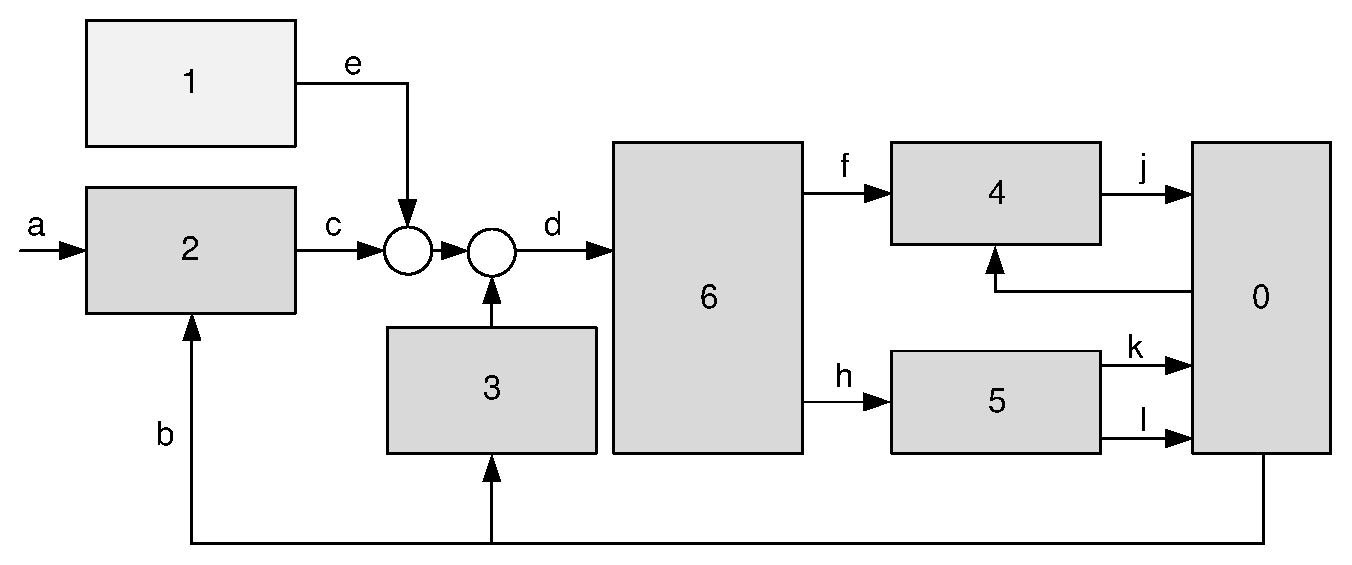
\includegraphics[width=1.\textwidth,clip, trim = 0cm 0cm 0cm 0cm]{2_Benzinmotor_Regelung.eps}
 \caption[Drehmomentorientierte Regelung eines Saugmotors]{Drehmomentorientierte Regelung eines Saugmotors mit dynamischer Aufteilung des gewünschten inneren Drehmoments in ein niederfrequentes Basisdrehmoment für die Luftfüllung $M_\text{ch}$ und ein hochfrequentes Zusatzmoment $M_\text{ig}$ für Zündwinkel und Einspritzdauer, vgl.\ \cite{isermann2010mechatronische}} % mit Pedalwert $\alpha_d$, Wunschantriebsmoment $M_d$, inneres Wunschmoment $M_{id}$, Basismoment $M_\text{ch}$, Zusatzmoment $M_\text{ig}$, Drosselklappenwinkel $\alpha_e$, Zündwinkel $\phi_\text{ig}$ und Einspritzdauer $t_i$}
 \label{fig:motor_funktionsweise}
\end{figure} 

Nach der anschließenden Verlustmomentkompensation der Motorsteuerung\index{Motorsteuerung}, die der inneren Verlustleistung des Motors Rechnung trägt, wird nun der große Vorteil eines Steuergeräts ausgespielt. Die stark verzögerte Reaktion des Motormoments auf Änderungen der Drosselklappe, die auf die Trägheit des angesaugten Luftstroms zurückzuführen ist, erweist sich nämlich als großer Nachteil für den Fahrer und vor allem für ein sicherheitskritisches Assistenzsystem wie eine Antriebs-Schlupf-Regelung (ASR). Einen unmittelbaren Einfluss auf das innere Motormoment besitzen hingegen die Zündung und Einspritzung, da sie kurbelwellensynchron arbeiten. Aus dem Grund erfolgt entsprechend \abb{fig:motor_funktionsweise} eine Aufteilung des gewünschten inneren Drehmoments  $M_{id}$ in ein niederfrequentes Basisdrehmoment $M_\text{ch}$ für die Luftfüllung, eingeregelt mittels Drosselklappenwinkel $\alpha_e$, und ein hochfrequentes Zusatzmoment $M_\text{ig}$, realisiert durch Veränderung des Zündwinkels $\phi_\text{ig}$ und der Einspritzdauer $t_i$ (s.\ Abb.\,\ref{fig:motor_funktionsweise}). Die jeweiligen Berechnungen basieren dabei auf der Invertierung des Drehmoment- bzw. Luftmassenmodells in Abhängigkeit verschiedener Messgrößen wie der Motordrehzahl $n$. \\
Auf Basis eines guten Motormodells ist es nun nicht nur möglich, vorgegebene Antriebsmomente umzusetzen, sondern auch das Schleppmoment (Motormoment bei $\alpha_d=0$) hinreichend genau zu schätzen, sodass es zum automatischen Verzögern im angeforderten Bremsmoment bereits berücksichtigt werden kann. Sowohl beim Soll- als auch Istwert des Antriebsmoments handelt es sich in modernen Fahrerassistenzarchitekturen bereits
%, wie auch schon bei den Bremsmomenten, 
um Radantriebsmomente, sodass die Getriebeübersetzung des aktuellen Gangs berücksichtigt ist. %Bei Automatikgetrieben erfolgt die Gangwahl nach sog.\ Schaltkennlinien, die im anschließenden Abschnitt erläutert werden.
%




\subsubsection{Funktionsweise der automatischen Getriebesteuerung\index{Getriebesteuerung}} %Differentialsteuerung
Aufgrund ihrer komfortsteigernden, effizienten und umweltschonenden Arbeitsweise sind Automatikgetriebe aus dem Antriebsstrang nicht mehr wegzudenken. Insbesondere bei der Realisierung von Komfortassistenzsystemen der Längsführung, namentlich das ACC, führen sie zu einer großen Entlastung, da andernfalls der Fahrer schalten muss.
Ohne ins Detail von dem aufwändigen elektro-mechanischen Aufbau und der Regelung einzelner Komponenten eines Automatikgetriebes zu gehen, soll das Automatikgetriebe auf seine aus Fahrerassistenzsicht wichtigsten Eigenschaften, definiert durch Momentübersetzung und Schaltpunkte, reduziert werden.

In Verbindung mit Motor und Differential legt das Automatikgetriebe über die Gangwahl das Antriebsmoment an den Reifen fest. Als Hauptkriterien stehen sich dabei das maximal entfaltbare Antriebsmoment und der möglichst geringe Verbrauch gegenüber \cite{gruhle2010steuerung}. Um den Kompromiss besser aufzulösen, werden dem Fahrer unterschiedliche Schaltprogramme (\zB \emph{Eco} und \emph{Sport}) angeboten. Davon unabhängig kann permanent über Kickdown die Maximalleistung des Motors abgefragt werden. \\
Die Gangwahl eines Schaltprogramms erfolgt über sog.\ Schaltkennlinien\index{Schaltkennlinie}, die einen bestimmten Gangwechsel (z.B.\ von 1 nach 2) in Abhängigkeit der Pedalstellung und der Geschwindigkeit auslösen, s.\ Abb.\,\ref{fig:getriebe}. Zur Vermeidung von Schaltpendeln unterscheidet sich die Kennlinie des Hoch- von der des Herunterschaltens, sodass eine Hysterese entsteht.
Zur Optimierung des Schaltvorgangs, welcher im Unterschied zum Handschalter unter Last erfolgt, wird neben dem Kupplungsdruck der jeweiligen Gänge auch eine Abschwächung des Motormoments angefordert \cite{gruhle2010steuerung}, s.\ \abschn{sec:motorregelung}.

\begin{figure}[h]
\newcommand{\smallsize}{.75}
	\psfrag{1}[cb][cb][\smallsize]{2-1}
	\psfrag{2}[cb][cb][\smallsize]{1-2}
	\psfrag{3}[cb][cb][\smallsize]{3-2}
	\psfrag{4}[cb][cb][\smallsize]{2-3}
	\psfrag{5}[cb][cb][\smallsize]{4-3}
	\psfrag{6}[cb][cb][\smallsize]{3-4}
	\psfrag{7}[cb][cb][\smallsize]{5-4}
	\psfrag{8}[cb][cb][\smallsize]{4-5}
	\psfrag{9}[cb][cb][\smallsize]{6-5}
	\psfrag{0}[cb][cb][\smallsize]{5-6}
	\psfrag{a}[cr][cr][\smallsize]{20}
	\psfrag{c}[cr][cr][\smallsize]{40}
	\psfrag{e}[cr][cr][\smallsize]{60}
	\psfrag{i}[cr][cr][\smallsize]{80}
	\psfrag{m}[cr][cr][\smallsize]{100}
	\psfrag{k}[cr][cr][1.]{KD}
	\psfrag{n}[ct][ct][\smallsize]{25}
	\psfrag{o}[ct][ct][\smallsize]{50}
	\psfrag{r}[ct][ct][\smallsize]{75}
	\psfrag{s}[ct][ct][\smallsize]{100}
	\psfrag{u}[ct][ct][\smallsize]{125}
	\psfrag{v}[ct][ct][\smallsize]{150}
	\psfrag{w}[ct][ct][\smallsize]{175}
	\psfrag{x}[ct][ct][\smallsize]{200}
	\psfrag{z}[ct][ct][\smallsize]{225}
	\psfrag{b}[ct][ct][1.0]{Geschwindigkeit / \unitfrac{km}{h}}
	\psfrag{y}[cb][cb][1.0]{Fahrpedalstellung / \%}
\centering
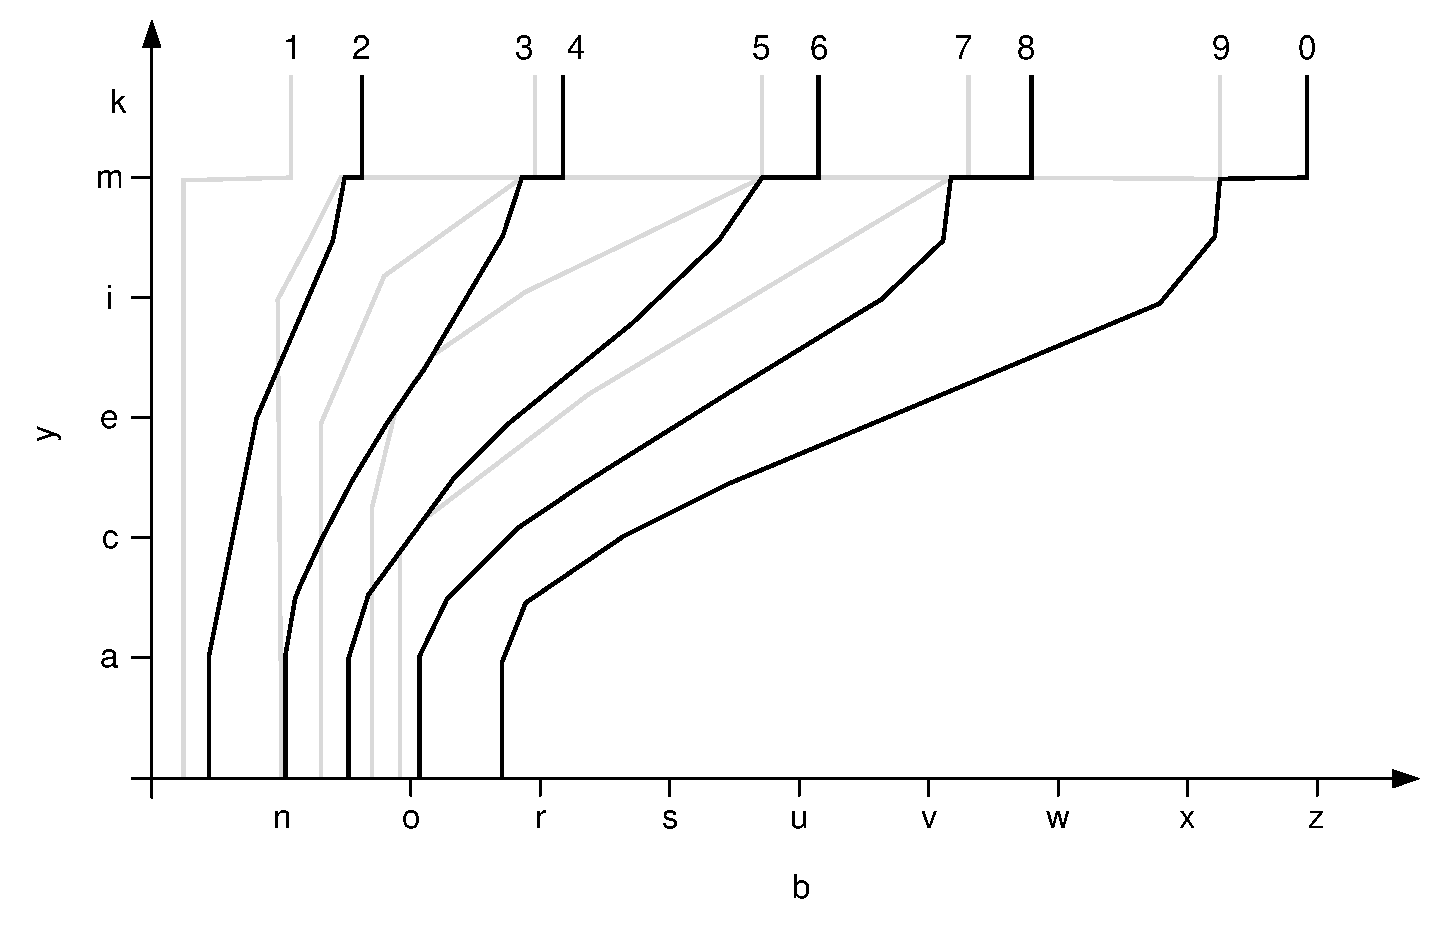
\includegraphics[width=1.0\textwidth,clip, trim = 0cm 0cm 0cm 0cm]{2_Getriebe_Schaltung.eps}
 \caption[Qualitativer Verlauf der Schaltkennlinien]{Qualitativer Verlauf der Schaltkennlinien eines 6-Gang-Automatikgetriebes \cite{gruhle2010steuerung}, Hochschalten in Schwarz, Herunterschalten in Grau, Kickdown (KD)}
 \label{fig:getriebe}
\end{figure} 


Für die Fahrerassistenz hat sich als Schnittstelle zum Antrieb, analog zum Radbremsmoment, das Gesamtantriebsmoment als Summe der angetriebenen Räder etabliert. Der damit verbundene Hauptvorteil liegt darin, dass aus Fahrerassistenzsicht kein Wissen über den Antriebsstrang vorhanden sein muss, da das Zusammenspiel aus Getriebe- und Motorsteuerung das Sollmoment bestmöglich umsetzt. 
Soll darüber hinaus die Antriebskraft unter den einzelnen Rädern umverteilt werden (es wird auch von \emph{torque vectoring} \cite{piyabongkarn2007use, fallah2012controller} gesprochen), so muss dies über ein sog.\ Sperrdifferential\index{Sperrdifferential}\footnote{Zur Unterscheidung beschreibt eine Differentialsperre eine hinzuschaltbare mechanische Verbindung, die keinerlei Drehzahlunterschied zwischen den Rädern zulässt.} erfolgen. Es bremst die Ausgleichsbewegung der einzelnen Räder und sorgt damit für eine, wenn auch verlustbehaftete Umverteilung der Antriebskraft. Insbesondere bei variierendem Fahrbahnuntergrund kann dadurch die Traktion deutlich verbessert werden.%, was genauer in \abschn{sec:torque_vectoring} erläutert wird.

Damit sind alle zur Realisierung aktiver Fahreingriffe verfügbaren Stellgrößen qualitativ beschrieben und es kann im nächsten Abschnitt auf die Systemeingangsgrößen eingegangen werden.




% Wie im eingangs genannten Stand der Technik beschrieben wird dabei aus dem Betätigungsgrad des Bedienelements des Fahrers unter Berücksichtigung wenigstens der Motordrehzahl ein vom Fahrer vorgegebener Sollmomentwert gebildet, der gegebenenfalls mit den von anderen Steuer- bzw. Regelsystemen gebildeten Momentwerten verglichen und ein Sollmomentwert ausgewählt wird, der zur Einstellung des Drehmoments der Brennkraftmaschine dient. Bezüglich der Einstellung der Luftzufuhr wird dabei, wie aus dem Stand der Technik bekannt, der Soll-Momentwert in einen Sollwert für die Zylinderfüllung umgewandelt, der wiederum in einen Sollwert für die Stellung der Drosselklappe umgewandelt wird. Zur Regelung des Ist-Moments auf das Sollmoment werden dann neben der Luftzufuhr in der aus der Stand der Technik bekannten Weise auch in die Zündwinkeleinstellung, die Kraftstoffzufuhr, etc. eingegriffen.


%Redundantes Signal für Last: Saugrohrdrucks bzw. des Luftmassenmessers Bei heutigen Steuersystemen werden wenigstens zwei Messeinrichtungen eingesetzt, beispielsweise ein Sensor zur Erfassung der Drosselklappenstellung und ein Sensor zur Erfassung der zuströmenden Luftmasse oder aber ein Sensor zur Erfassung des Saugrohrdrucks.
% http://www.patent-de.com/20071122/DE19812485B4.html



\section{Sensorik, Mess- und Schätzgrößen}
Sowohl die Trajektorienoptimierung als auch ein Großteil der unterlagerten Regler beruhen auf dem Prinzip der Zustandsrückführung (im Unterschied zur Ausgangsrückführung). Es verwundert in der Praxis daher nicht, dass das Leistungsvermögen des Gesamtsystems maßgeblich von der Qualität der Sensorik und Messgrößenaufbereitung bestimmt wird. Schließlich kann das Fahrzeug weitaus bessere Entscheidungen über die einzuschlagende Trajektorie treffen, wenn es genaue Kenntnis über seinen eigenen Fahrzustand und den anderer Verkehrsteilnehmer (Abstand, Bewegungsrichtung etc.) besitzt. Zugleich wird die Stabilisierungsebene durch ein latenzarmes Messsignal dazu befähigt, auf Störungen schnell zu reagieren, um eine optimierte Trajektorie möglichst genau umzusetzen. Im Folgenden wird daher die den Assistenzfunktionen im Fahrzeug zur Verfügung stehende Information beschrieben und ein kurzer Einblick in die für sie wesentlichen Aspekte der Entstehung gegeben. Die Einteilung in Eigenfahrzeug- (im Folgenden mit Ego bezeichnet) und Fahrzeugumfeld-bezogene Information erweist sich hierbei als zweckmäßig.

%Grundsätzlich kann über die Mess- und Schätzgrößen in eigenfahrzeugbezogene und umweltbezogene unterschieden werden
% correvit
\label{sec:sensoren} % Lenkwinkelsensor

\subsection{Fahrzustandserfassung\index{Fahrzustandserfassung}} \label{sec:eigenfahrzustandserfassung}
So wie der menschliche Fahrer über seine vestibuläre\footnote{Das Gleichgewichtsorgan wird auch als Vestibularapparat bezeichnet.} und visuelle Wahrnehmung muss ein Assistenzsystem über die Fahrzeugsensorik den aktuellen Fahrzustand erfassen und das möglichst präzise. Hierzu steht ihm insbesondere die Inertialsensorik zur Verfügung, welche im Fahrzeug als sog.\ \emph{Sensorcluster} die Beschleunigungen und Drehraten in den für die Fahrdynamik relevanten Richtungen misst. Darüber hinaus sind mit der gewonnenen Messinformation unter Einbezug weiterer Messgrößen die Fahrzeuglängs- und Quergeschwindigkeit zu schätzen, da sie aus Kostengründen in Serienfahrzeugen nicht direkt gemessen werden.

\subsubsection{Funktionsweise Sensorcluster\cite{Sensorcluster}}
Während für Stabilitätsprogramme wie das ESP neben der Quer- und Längsbeschleunigung die Drehrate um die Fahrzeughochachse als Messgröße ausreichend ist, erfordern automatische Überrollschutzsysteme von Fahrzeugen mit erhöhtem Schwerpunkt zusätzlich die Erfassung der Drehrate um die Fahrzeugquer- und -längsachse. Das sog.\ \emph{Sensorcluster} umfasst nun zentral die entsprechend ihrer Messachsen %der jeweiligen Messgröße 
ausgerichteten Beschleunigungs-\index{Beschleunigungssensor} und Drehratensensoren \index{Drehratensensor} und stellt deren Messsignale auf dem Fahrzeug-Bus den Steuergeräten zur Verfügung \cite{reif2010sensoren}. 
\begin{figure}[ht]
\newcommand{\smallsize}{.75}
	\psfrag{f}[cl][cl][1.0]{$F_a$}
	\psfrag{b}[cr][cr][1.0]{Auslenkung}
	\psfrag{m}[cc][cc][1.0]{$m$}
	\psfrag{a}[cr][cr][1.0]{$a$}
\centering
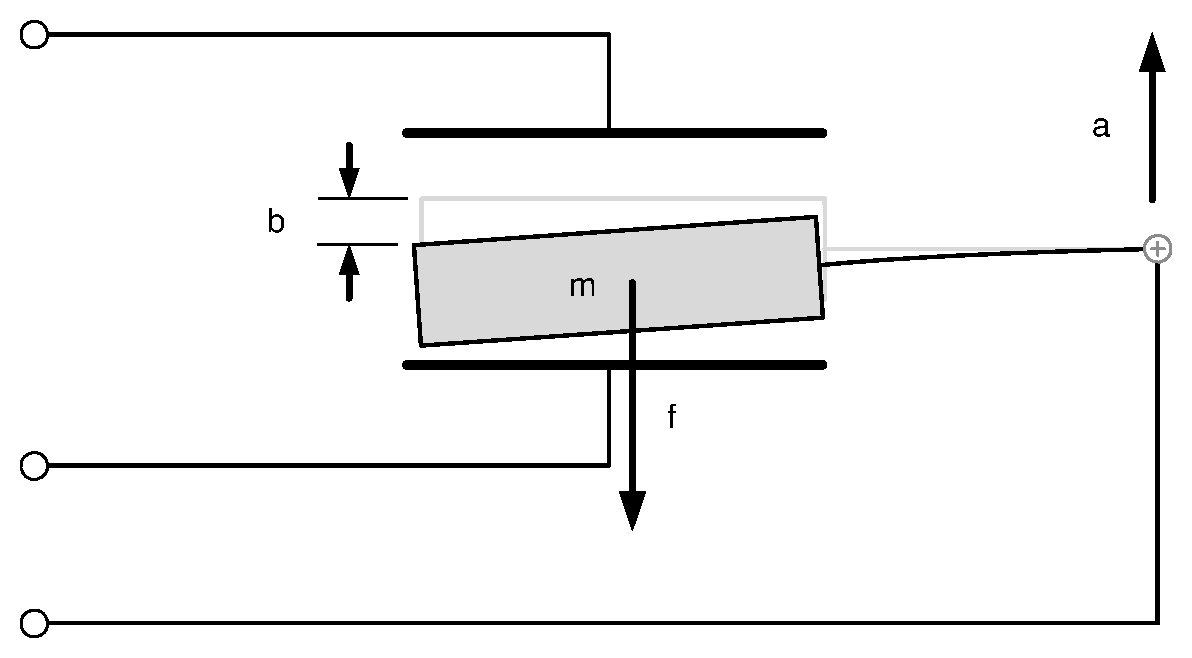
\includegraphics[width=.5\textwidth,clip, trim = 0cm 0cm 0cm 0cm]{2_querbeschleunigungssensor.eps}
 \caption[Funktionsweise eines Beschleunigungssensors]{Funktionsweise eines mikro-elektro-mechanischen Beschleunigungssensors: Aufgrund der zu messenden Beschleunigung $a$ erfährt die Masse $m$ eine Messkraft $F_a$, die zu einer zur Beschleunigung proportionalen Auslenkung führt \cite{reif2010sensoren}.}
 \label{fig:querbeschleunigungssensor}
\end{figure}
%
Im Automobilbereich haben sich sog.\ \emph{mikro-elektro-mechanische} (MEM) Beschleunigungs- und Drehratensensoren etabliert, die aus filigranen mechanischen Silizium-Strukturen und elektronischen Auswerteeinheiten bestehen. Zwar unterscheiden sich die Sensoren im Aufbau von Hersteller zu Hersteller, in ihrer grundsätzlichen Funktionsweise decken sie sich jedoch. Zur Erklärung sei \abb{fig:querbeschleunigungssensor} betrachtet, in der 
das Messprinzip der Querbeschleunigung verdeutlicht wird. Die elastisch gelagerte Masse $m$ erfährt bei einer Beschleunigung $a$ die Trägheitskraft $F_a$, was zu einer kapazitiv messbaren Auslenkung führt, sodass über die Federsteifigkeit und Masse auf $a$ geschlossen werden kann. Alternativ wird die Masse durch eine schnelle Lageregelung in ihrer Position gehalten, womit die erforderliche Kompensationskraft der Regelung der Trägheitskraft entspricht. Das erhöht den Messbereich (Amplitude und Grenzfrequenz), da die Masse sehr nahe am Nullpunkt der Auslenkung bleibt und somit ein lineares Systemverhalten gewährleistet ist.  \\
%

Die Messung der Drehrate erfolgt ebenfalls unter Ausnutzung von Trägheitseffekten. Allerdings werden hierzu zwei miteinander verbundene Masseschwinger angeregt, sodass sie gegensätzlich in ihrer gemeinsamen Resonanzfrequenz ($\approx \unit[1]{kHz}$) schwingen, s.\ \abb{fig:stimmgabe_gyro}. Bei einer Drehbewegung $\Omega$ senkrecht zur Oszillationsbewegung erfahren dann die Massen die Coriolis-Kraft, was eine Schwingung aus der Ebene heraus mit einer Amplitude proportional zur Gierrate induziert, die wiederum elektrostatisch gemessen werden kann \cite{reif2010sensoren}.
\begin{figure}[h]
\newcommand{\smallsize}{.75}
	\psfrag{2}[cc][cc][1.0]{$\Omega$}
	\psfrag{a}[ct][ct][1.0]{Anregung}
	\psfrag{c}[cl][cl][1.0]{Coriolis-Kraft}
	\psfrag{t}[ct][ct][1.0]{$t$}
	\psfrag{b}[cl][cl][1.0]{\parbox[r]{1.5cm}{Induzierte \\ Schwingung}}
\centering
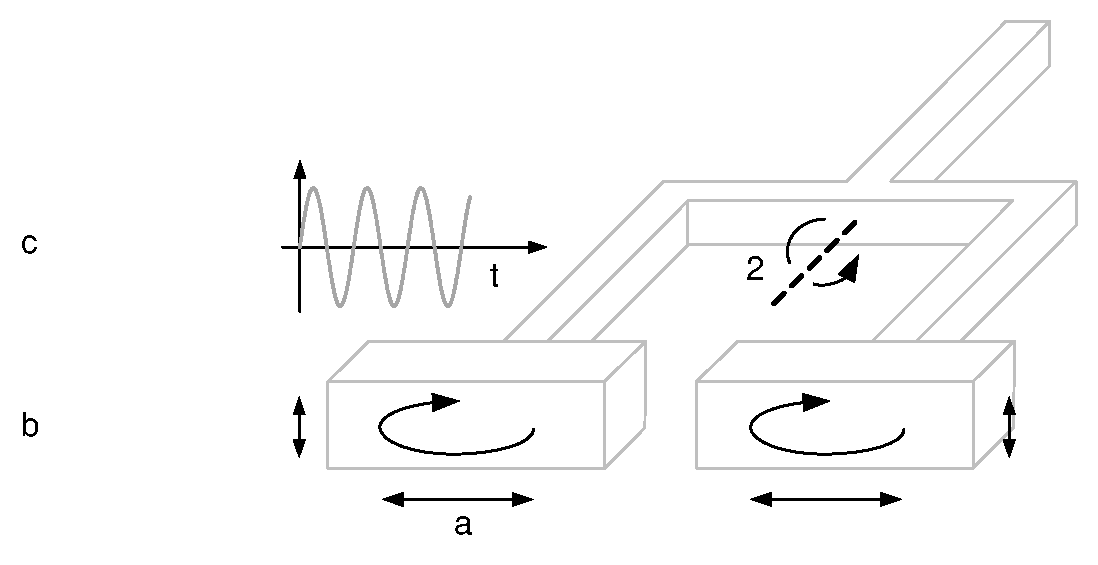
\includegraphics[width=.75\textwidth,clip, trim = 0cm 0cm 0cm 0cm]{2_stimmgabe_gyro.eps}
 \caption[Funktionsweise eines Drehratensensors]{Funktionsweise eines mikro-elektro-mechanischen Drehratensensors: Durch die Coriolis-Kraft erfahren die zur Oszillation angeregten Massen eine der Drehrate $\Omega$ proportionale Querauslenkung \cite{reif2010sensoren}.}
 \label{fig:stimmgabe_gyro}
\end{figure}


\subsubsection{Geschwindigkeits-\index{Geschwindigkeitsschätzung} und Schwimmwinkeschätzung\index{Schwimmwinkeschätzung}} \label{sec:beta_v} % not my business -> Literaturverweis
Da die Dynamik des Fahrzeugs grundlegend von seiner Geschwindigkeit beeinflusst wird, erfordern die meisten Assistenzfunktionen ein genaues Längsgeschwindigkeitssignal $v_x(t)$. Gerade aber im fahrphysikalischen Grenzbereich weisen die Reifen erheblichen Schlupf\footnote{Die normierte Geschwindigkeitsdifferenz zwischen Fahrbahn und Reifen in der Kontaktfläche wird als Schlupf bezeichnet.} auf, sodass von den Raddrehzahlsensoren (s.\ \cite{reif2010sensoren}) nur unzureichend auf die Fahrzeuggeschwindigkeit geschlossen werden kann. Ebenso verhält es sich bei der Fahrzeugquergeschwindigkeit $v_y(t)$, die bei einem schleudernden Fahrzeug ganz erhebliche Werte annehmen kann. Wenn auch im Rennsport und Erprobungsbetrieb Geschwindigkeitsmesssysteme über Grund verwendet werden (optisch \cite{horn2006zweidimensionale} oder mittels hoch genauer, GPS-gekoppelter Inertialsensorik \cite{ryu2004integrating}), so verbietet sich aus Kostengründen deren Einsatz im Serienfahrzeug. Da aufgrund des Messrauschens bei einer reinen Aufintegration der Drehraten- und Beschleunigungssignale die Genauigkeit rapide abnimmt, müssen die Geschwindigkeiten geschätzt werden, was der Zuhilfenahme von Fahrzeugmodellen bedarf. \\
Die Längsgeschwindigkeitsschätzung erfolgt so, dass auch während einer ABS-Bremsung einzelne Räder gezielt "`unterbremst"' werden und dadurch nach kurzer Zeit stabil laufen. Aus der sich dann ergebenden Raddrehzahl kann über das anliegende Radbremsmoment (s.\ \abschn{sec:ehb_funktionsweise}) und die Reifencharakteristik auf die Geschwindigkeit über Grund geschlossen werden. Unter Berücksichtigung des Lenkwinkels und der Giergeschwindigkeit wird dann die Umrechnung in den Schwerpunkt vorgenommen. Über die Differentialgleichung der Längsgeschwindigkeit erfolgt die Sensorfusion mittels erweitertem Kalman-Filter\index{Kalman-Filter} \cite{kalman1960new}, s.\, \cite{BHB2012_vanZanten_bremsanlage}. \\
Ähnlich verhält es sich bei der Querbewegung, wobei i.\,Allg.\ anstelle von $v_y$ die zum Fahrzeug relative Bewegungsrichtung
\begin{align*}
	\beta = \arctan(v_y/v_x)\;,
\end{align*}
der sog.\ \emph{Schwimmwinkel}\index{Schwimmwinkel}, als Zustandsgröße herangezogen wird, s.\ \abb{fig:fahrzeugbewegung}. Analog zur Längsgeschwindigkeitsschätzung wird über die Differentialgleichung der Querbewegung der Schwimmwinkel mittels erweitertem Kalman-Filter aus der Fahrzeugdrehrate um die Hochachse, der Querbeschleunigung und dem Lenkwinkel geschätzt \cite{tno2007_stateestimator, BHB2012_vanZanten_bremsanlage, Konig2008}.
\begin{figure}[h]
\centering
\newcommand{\smallsize}{.85}
	\psfrag{x}[tc][tc][1.0]{$x_1$}
	\psfrag{y}[rc][rc][1.0]{$x_2$}
	\psfrag{m}[tl][tl][1.0]{$v_y$}
	\psfrag{n}[tl][tl][1.0]{$v_x$}
	\psfrag{b}[cc][cc][1.0]{$\beta$}
	\psfrag{p}[cc][cc][1.0]{$\psi$}
	\psfrag{v}[rb][rb][1.0]{$v$}
	\psfrag{t}[lb][lb][1.0]{$\theta$}
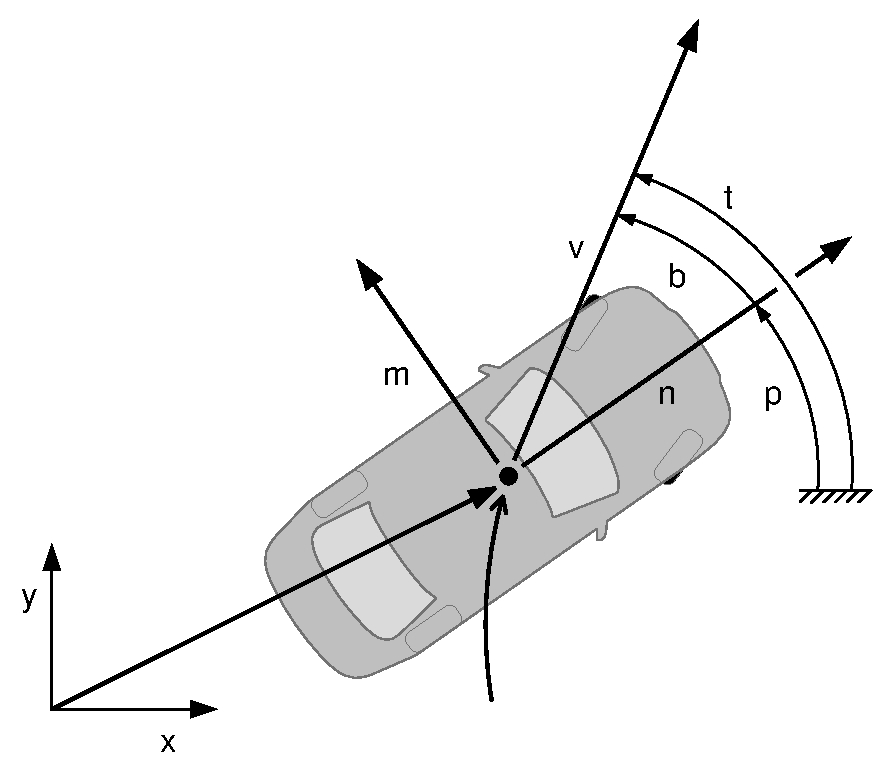
\includegraphics[width=.55\textwidth,clip, trim = 0cm 0cm 0cm 0cm]{2_Kinematik.eps}
 \caption[Bewegungskinematik des Fahrzeugs]{Bewegungskinematik des Fahrzeugs innerhalb eines ortsfesten Koordinatensystems $[x_1, x_2]$}
 \label{fig:fahrzeugbewegung}
\end{figure} 



\subsection{Eigenlokalisierung\index{Eigenlokalisierung}}
Wie bereits 1986 praktisch nachgewiesen wurde \cite{dickmans1989sod}, kann bei vorhandenen Fahrbahnmarkierungen ein Fahrzeug der Spur selbständig folgen, und das ohne jegliche Art einer globalen Eigenlokalisierung. Schließlich reicht es aus, wenn regelmäßig die Fahrzeugrelativposition und -ausrichtung zu den Spurmarkierungen aus einer Kamera bestimmt und Abweichungen von der so bestimmten Fahrbahnmitte über Lenkbefehle minimiert werden\footnote{Eine Alternative stellt das Einlassen von stromdurchflossenen Drähten oder das Einschlagen von Magneten in die Fahrbahn dar, s.\ beispielsweise\ \cite{markgraf2002autonomes, tan1999development}.}. Die Robotik verwendet hierfür auch den Begriff \emph{visual servoing}\index{visual servoing} \cite{allen1991real}, da Regelabweichungen direkt aus dem Sensor bezogen werden. Dasselbe Prinzip findet in Fahrzeuglängsrichtung in der serienmäßig verfügbaren Komfortfunktion ACC ebenfalls Anwendung \cite{venhovens2000stop}, die mit dem nach vorne gerichteten Radar die Relativbewegung zum Vorderfahrzeug vermisst und einen vorgegebenen Abstand automatisch über Brems- und Motoreingriffe einregelt. Problematisch wird es allerdings, wenn bereits für kurze Zeit die Regelgrößen nicht verfügbar sind (z.B.\ kurzzeitiges Gegenlicht beim Spurhalten), da dann aufgrund der fehlenden Messgröße vom Regler keine Stellgröße berechnet werden kann. \\
Für einige Anwendungen im Fahrzeug verbietet sich gar funktionsbedingt das Prinzip des visual servoing. So kann zwar ein Einparkassistent durch einen  seitlichen Sensor die Größe und Relativposition einer Parklücke bei der Vorbeifahrt gut bestimmen, während des Manövers ist diese Information aber aufgrund der veränderten Sensorperspektive nicht verfügbar, sodass die Position relativ zur Parklücke anderweitig geschätzt werden muss. Ähnlich verhält es sich beim Ausweichen, während dessen eine nach vorne gerichtete Sensorik aufgrund der starken Drehbewegung um die Fahrzeughochachse (das sog.\ Gieren) kurz nach dem Auslenken das Hindernis verliert. Die übergeordnete Fragestellung ist in den Situationen demnach, wohin sich das Hindernis oder die Spur relativ zum Fahrzeug innerhalb des letzten Zeitabschnitts bewegt haben. Um das zu beantworten, bietet es sich an, mit Hilfe der geschätzten Egobewegung und fahrzeugfester Umfeldsensorik die Hindernisbewegung über Grund zu ermitteln, über der Zeit zu verfolgen \cite{maurer2005fahrerassistenzsysteme} und, falls erforderlich, zu prädizieren. Wenn auch noch die geschätzte Egobewegung aufintegriert wird, dann kann trotz kurzzeitig verdecktem Hindernis auf dessen Relativposition zum Fahrzeug geschlossen werden. Die Aufintegration wird auch als Koppelnavigation\index{Koppelnavigation} bezeichnet und in \abschn{sec:koppelnavi} erläutert. \\
%eine Aufteilung der Relativbewegung in Fahrzeugeigen- und Hindernisbewegung (letztere trivial bei statischen Hindernissen) über Grund an, eine Herangehensweise, die sich nicht nur bei hochautomatisierten Fahrzeugen (s.\ \zB \cite{jfr2008}) bewährt hat, weil hierdurch ganz allgemein die Hindernisbewegung besser gefiltert werden kann\footnote{Wird auch als Tracking bezeichnet \cite{todo}}. 
%An dieser Stelle sei bereits angemerkt, dass e
Sollen hingegen global referenzierte Informationen wie Straßenkarten herangezogen werden, dann ist zusätzlich eine globale Positionsbestimmung (beispielsweise über GPS) erforderlich, was in \abschn{sec:globalelok} beleuchtet wird. 
%Da die Hindernisbewegung im Rahmen der Situationsprädiktion noch genauer in Abschn.\,\ref{sec:praediction} beleuchtet wird, soll an dieser Stelle die Bestimmung der Eigenbewegung und Positionierung ausgeführt werden.

\subsubsection{Lokale Bestimmung von Egoposition und -ausrichtung} \label{sec:koppelnavi}
Ungeachtet der Ursache einer Bewegung beschäftigt sich die Kinematik mit der Bewegung von Körpern im Raum und ist damit Grundlage der Fahrzeugbewegung. Zur Beschreibung der rotatorischen und translatorischen Bewegung in der Ebene reicht die Geschwindigkeit $v$ eines fahrzeugfesten Referenzpunkts über Grund sowie dessen aktuelle Bewegungsrichtung $\theta$ (Kursrichtung\index{Kursrichtung}) und die Fahrzeugorientierung\index{Fahrzeugorientierung} $\psi$ aus, wobei  $\theta$ und $\psi$ relativ zu einem ortsfesten Koordinatensystem definiert werden. Wie anhand von Abb.\,\ref{fig:fahrzeugbewegung} nachvollzogen werden kann, genügt die Position $[x_1, x_2]$ dann der Differentialgleichung
\begin{align*}
	\dot x_1 &= v \cos\theta \\
	\dot x_2 &= v \sin\theta\,.
\end{align*}
Der Kurswinkel wiederum lässt sich aufteilen in
%In den meisten Anwendungen fehlt allerdings eine absolute Orientierungsreferenz, sodass $\theta$ und $\psi$ unbekannt sind und geschätzt werden müssen\footnote{Dasselbe gilt für $v$ im Fall von hochdynamischen Fahrmanövern, bei denen aufgrund des starken Schlupfs die Raddrehzahlen nicht unmittelbar die Fahrzeugbewegung spiegeln, s.\ Abschn.\,\ref{todo:ABS}.}. Hierzu bietet sich die Aufteilung des Kurswinkels in
\begin{align*}
	\theta = \psi + \beta\, ,
\end{align*}
wobei $\beta$ die Bewegungsrichtung relativ zum Fahrzeug beschreibt, s.\ Abb.\,\ref{fig:fahrzeugbewegung}. Falls der Bezugspunkt im Fahrzeugschwerpunkt liegt, wird $\beta$ auch als Schwimmwinkel\index{Schwimmwinkel} bezeichnet, s. \abschn{sec:beta_v}. \\
%
%  Dieser kann entweder optisch gemessen (s.\ Correvit, Visual Odometrie) oder unter Einbezug der Fahrphysik geschätzt werden (s.\ Abschn.\ref{sec:}). 
Ist auf eine direkte Bestimmung der Fahrzeugausrichtung, etwa durch einen Kompass, zu verzichten, so muss zusätzlich die Fahrzeuggierrate\index{Gierrate} $r=\dot \psi$ gemessen oder geschätzt\footnote{Bei langsamer Fahrt liefert das kinematische Einspurmodell eine sehr genaue Schätzung für die Gierrate, s.\ \abschn{sec:anhaengerdynamik}.} werden, und es ergibt sich insgesamt die Fahrzeugbewegung zu
\begin{align*}
	\dot x_1 &= v \cos(\psi + \beta) \\
	\dot x_2 &= v \sin(\psi + \beta) \\
  \dot   \psi &= r \,.
\end{align*}
Die sog.\ Koppelnavigation\index{Koppelnavigation} (engl.\ \emph{dead reckoning}) stellt nun nichts weiter dar, als die Aufintegration der drei\footnote{In der Schifffahrt, dem Ursprung der Koppelnavigation, entfällt die letzte Gleichung, da dort ein Kompass verwendet werden kann, dessen Einsatz sich aufgrund von Feldstörungen im Fahrzeug verbietet. Die relative Fahrtrichtung $\beta$ über Grund wird durch die sog.\ \emph{Beschickung} berücksichtigt, welche der Versetzung durch Strömung und Wind Rechnung trägt \cite{dreyer_sks}.} Differentialgleichungen, was problemlos numerisch erfolgen kann. Da die Raddrehzahlen in die Geschwindigkeit eingehen, wird in dem Zusammenhang in der Fahrerassistenz häufig auch der Ausdruck \emph{Odometrie\index{Odometrie}}\footnote{Positionsbestimmung anhand der zurückgelegten Wegstrecke; bei Schätzung der Fahrzeugbewegung aus der Kamera wird gar von \emph{visual odometry} gesprochen \cite{lategahn2012motion}.} gebraucht.

Bei der Aufintegration akkumulieren sich allerdings über der Zeit das Sensorrauschen von $r$, der Schätzfehler in der Geschwindigkeit $v$ und dem Schwimmwinkel $\beta$ sowie die numerischen Ungenauigkeiten auf. Dieses als \emph{Drift}\index{Drift} bezeichnete Phänomen ist in Abb.\,\ref{fig:Odo_drift} aus der Sicht einer Fahrerassistenzfunktion verdeutlicht. Dabei wird die Ursprungsposition (weißes Fahrzeug) mit der aktuellen Fahrzeugposition (graues Fahrzeug) durch die tatsächlich gefahrene Trajektorie (schwarze Linie) verbunden. Aufgrund der mit der Koppelnavigation verbundenen Fehler verschlechtert sich die Positions- und Orientierungsschätzung je länger die Fahrt andauert, sodass die vermeintlich gefahrene Trajektorie (grau) immer stärker von der tatsächlichen abweicht. Genauer gesagt: Kehrt das Fahrzeug wieder zum mutmaßlichen Ursprung der Trajektorie zurück, so weicht es dann um den aktuellen Drift in seiner Position und Ausrichtung von den eigentlichen Werten ab. \\
Für viele Anwendungen stellt der auf den Drift zurückzuführende Fehler jedoch kein Problem dar, weil sich die meisten Assistenzfunktionen lediglich auf Zeitpunkte zurückbeziehen, die nicht weit in der Vergangenheit liegen (s.\ kleine und große Ellipsen in Abb.\,\ref{fig:Odo_drift}).

\begin{figure}[h]
\newcommand{\smallsize}{.85}
\psfrag{N}[rc][rc][\smallsize]{Nord}
\psfrag{O}[tr][tr][\smallsize]{Ost}
\psfrag{d}[tr][tr][\smallsize]{Drift}
\psfrag{m}[br][br][1.0]{$T_\text{glob}(0)$}
\psfrag{n}[tl][tl][1.0]{$T_\text{glob}(t)$}
\psfrag{s}[cl][cl][\smallsize]{Ortsfestes KOS}
\psfrag{x}[cr][cr][\smallsize]{vermeintliche Trajektorie}
\psfrag{z}[cl][cl][\smallsize]{tatsächliche Trajektorie}
	\psfrag{1}[tl][tl][\smallsize]{\parbox[c]{7cm}{\begin{flushleft} großer \\ Fehler \end{flushleft}}}
		\psfrag{0}[bc][bc][\smallsize]{\parbox[c]{7cm}{\begin{center} kleiner \\ Fehler \end{center}}}
\psfrag{q}[tr][tr][\smallsize]{\parbox[c]{1cm}{\begin{centering} Fahrzeugfestes \\ KOS \end{centering}}}
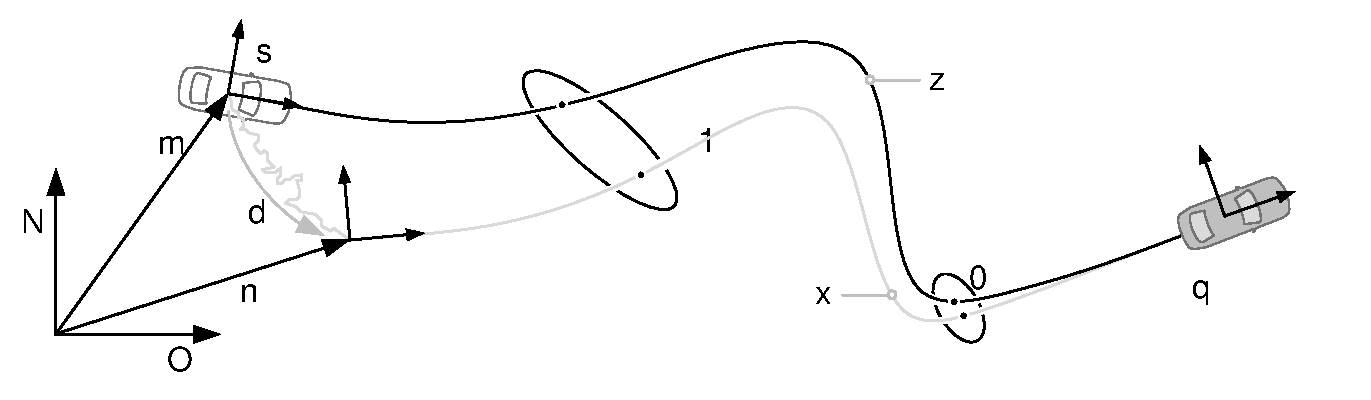
\includegraphics[width=1.\textwidth,clip, trim = 0cm 0cm 0cm 0cm]{2_koppelnavi_drift.eps}
 \caption[Mit Drift verbundene ortsfeste Koordinaten]{Veranschaulichung der mit Drift verbundenen ortsfesten Koordinaten}
 \label{fig:Odo_drift}
\end{figure} 

 

\subsubsection{Globale Bestimmung von Egoposition und -ausrichtung} \label{sec:globalelok}
Für die Umsetzung moderner Assistenzfunktionen der Führungsebene sind detaillierte Umfeldinformationen\index{Umfeldinformationen} wie zukünftiger Straßenverlauf und Vorfahrtsregelungen vonnöten, die durch aktuelle Umfeldsensorik und deren Auswertealgorithmik nur unzureichend zur Verfügung gestellt werden können. Insbesondere die im Rahmen der DARPA Urban Challenge\index{DARPA Urban Challenge} entstandenen Arbeiten  \cite{urmson2008adu, montemerlo2008junior, bacha2008odin, jfr2008} belegen jedoch, dass ein solches Defizit größtenteils durch global-referenzierte Daten ausgeglichen werden kann. Maßgeblich für die Verlässlichkeit der Karteninformation\index{Karteninformation} ist dabei neben der Genauigkeit vor allem deren Aktualität. Während es ausreichend sein kann, die Straßeninformation außerhalb von Baustellen nur einmal am Tag auf dem Fahrzeug zu aktualisieren, erfordern dynamische Gefahrenquellen, wie liegen gebliebene Fahrzeuge oder gar an eine Kreuzung herannahende Fahrradfahrer, eine permanente, latenzarme Informationsübertragung mittels Fahrzeug-zu-Fahrzeug- oder Fahrzeug-zu-Infrastruktur-Kommunikation (Car-to-X, kurz C2X), s.\ beispielsweise \citeltex{eichhorn2013Maneuverprediction, Werling_Vernetzung2012}. \\
Unabhängig von der Aktualisierungsrate ist es zur Nutzung der übermittelten Karteninformation wichtig zu wissen, an welcher Stelle der Karte und mit welcher Ausrichtung sich das Egofahrzeug befindet, was wiederum eine hinreichend genaue Bestimmung der globalen Fahrzeugposition und -ausrichtung erfordert. \\
Eine Möglichkeit hierfür stellt die Verwendung von GPS (Global Positioning System\index{Global Positioning System}) dar, das  
schon heute die Unterstützung des Fahrers durch Navigationsgeräte ermöglicht. Die Qualität und Verfügbarkeit von GPS unterliegt insbesondere im städtischen Bereich jedoch starken Schwankungen, sodass nach Alternativen gesucht wird 
\cite{pink2010bildbasierte, geiger2012we,levinson2010robust}. Für Hilfestellung sorgt hierbei die Robotik mit einer Vielzahl 
von Lokalisierungsverfahren \cite{borenstein1997}, die mittels Laserscannern \citeltex{Levinson2011} und Videokameras \cite{lategahn2013mapping} die Umgebung 
erfassen und geeignete Landmarken\index{Landmarke} bestimmen. Sind deren Positionen ebenfalls in einer Karte verzeichnet, kann über Triangulation auf die Roboterposition und -ausrichtung geschlossen\footnote{Erfolgt die Kartenerstellung auf Basis der gleichzeitigen Schätzung der Position aus Umfelddaten, so wird von \emph{simultaneous localization and mapping \index{simultaneous localization and mapping}} (SLAM) gesprochen, s.\ beispielweise \cite{Thrun2005, geiger2012we, kohlhepp2007elastic}.} und das Ergebnis mit der lokalen Positionsschätzung des vorherigen Abschnitts fusioniert werden. Angesichts der vermehrt eingesetzten Umfeldsensoren im Fahrzeug wird eine solche landmarkenbasierte Lokalisierung auch für die Fahrerassistenz interessant, sodass auf serientaugliche Alternativen zum GPS in den nächsten Jahren zu hoffen ist.

In der Funktionsarchitektur ist grundsätzlich bei der Wahl der Koordinatenursprünge darauf zu achten, dass sich Korrektursprünge der globalen Eigenlokalisierung nur auf Module auswirken, die auch wirklich auf eine absolute Position und Ausrichtung angewiesen sind. Eine saubere Trennung zwischen lokalen und globalen Koordinatensystemen, wie sie in \ref{app:kos} vorgeschlagen wird, ist daher unabdingbar.




\subsection{Fahrzeugumfeld-Modellierung und -Prädiktion}
Während für Assistenzsysteme der Stabilisierungsebene wie ESP die Schätzung des eigenen Fahrzeugzustands ausreicht (s.\ Abschn.\,\ref{sec:eigenfahrzustandserfassung}), so erfordert die Realisierung von Komfort- und Sicherheitsfunktionen der Führungsebene noch zusätzlich die Erfassung des Fahrzeugumfelds. Bereits heute ist eine Fülle von Umfeldsensorik im Serieneinsatz, namentlich Video\index{Video}, Radar\index{Radar}, Lidar\index{Lidar} und Ultraschall\index{Ultraschall}, deren jeweilige Messinformationen aufgrund unterschiedlicher Genauigkeiten und Erfassungsbereiche fusioniert werden. Angesichts der steigenden Funktionsanzahl im Fahrzeug ist es hierbei jedoch erstrebenswert, von einer funktionsspezifischen Sensordatenverarbeitung abzukommen, wie sie in der Serie aktuell gang und gäbe ist, und stattdessen die Messinformation zu einem generellen Abbild der Verkehrsszene zu fusionieren. Es kann dann als sog.\ \emph{Umfeldmodell\index{Umfeldmodell}} \cite{mahlisch2009filtersynthese} den verschiedenen Assistenzfunktionen zentral bereitgestellt werden. \\
Die Fahrzeugumfeld-Erfassung stellt allerdings eines der umfangreichsten Kapitel der Fahrerassistenz dar, sodass an dieser Stelle nur auf deren grundsätzlichen Aufbau und die für die Führungsebene wichtigsten Aspekte eingegangen werden kann. Zu letzteren zählen vor allem die Repräsentationsform der Hindernisse und der geschätzten Zustände einschließlich Unsicherheiten. %, da das Umfeldmodell der Manöverplanung als wichtige Schnittstelle dient. 
Welche Einzelschritte erforderlich sind, um von der zu jedem Messzeitpunkt erfassten Rohsensordateninformation zu einer Zustandsschätzung und Prädiktion der Umfeldobjekte zu gelangen, wird nun kurz skizziert. \\

\subsubsection{Mehrobjektverfolgung\index{Mehrobjektverfolgung}}
Nahezu alle bekannten Verfahren der \emph{Mehrobjektverfolgung} entsprechen der in \abb{fig:Klassische_Systemarchitektur_Tracking} dargestellten Systemarchitektur \cite{mahlisch2009filtersynthese}. In ihr werden im ersten Schritt die Rohdaten der Umfeldsensorik (Kamerabild \cite{dang2007kontinuierliche}, Lidar-Punktewolke \cite{moosmann2012interlacing}, Radar-Echo \cite{Diewald2013} etc.) auf Merkmale untersucht, die für die jeweilig zu erfassende Hindernisklasse (z.B. Fahrzeug, Fußgänger) sprechen. Das Ergebnis dieser \emph{Objektdetektion} ist eine Liste individuell erkannter Objekte, die im anschließenden Schritt der \emph{Objektassoziation} den bereits aus vorangegangenen Messungen verfolgten Hindernissen zugeordnet werden müssen.
Die Bewegungsschätzung eines jeden Objekts erfolgt anschließend unter Verwendung eines \emph{Zustandsfilters}, in dessen sog.\ Filterinnovation die von der Assoziation dem Objekt zugeordneten Messungen eingehen. Hierbei ist die Bewegung des Eigenfahrzeugs, s.\ \abschn{sec:eigenfahrzustandserfassung}, zu berücksichtigen.
\begin{figure}[h]
\newcommand{\smallsize}{.5}
	\psfrag{a}[cc][cc][1.0]{Objektdetektion}
	\psfrag{c}[cc][cc][1.0]{Objektassoziationen}
	\psfrag{e}[cc][cc][1.0]{Zustandsfilterung}
	\psfrag{m}[cc][cc][1.0]{Validierung}
	\psfrag{1}[cl][cl][1.0]{Sensorrohdaten}
	\psfrag{2}[cl][cl][1.0]{Objektliste}
	\psfrag{7}[cr][cr][1.0]{Assoziationen}
	\psfrag{4}[cl][cl][1.0]{Track-Liste}
	%\psfrag{5}[lc][lc][1.0]{Track-Verwaltung}
	\psfrag{6}[cl][cl][1.0]{Dyn.\ Umfeldmodell}
	\psfrag{3}[cl][cl][1.0]{Prädiktionen}
	\centering
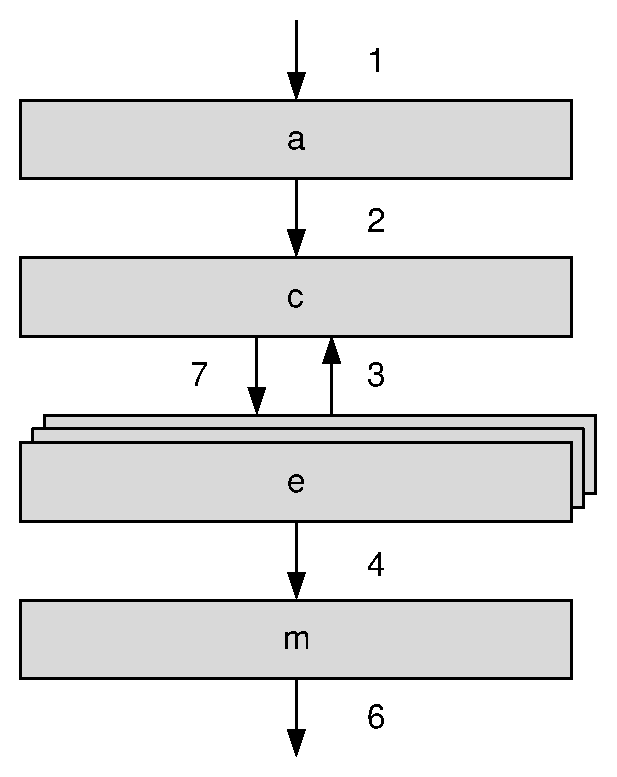
\includegraphics[width=.4\textwidth,clip, trim = 0cm 0cm 0cm 0cm]{2_Klassische_Systemarchitektur_Tracking.eps}
 \caption[Einzelmodule in der Mehrobjektverfolgung]{Vereinfachte Darstellung der Einzelmodule in der Mehrobjektverfolgung, s.\ auch \cite{mahlisch2009filtersynthese}}
 \label{fig:Klassische_Systemarchitektur_Tracking}
\end{figure}

Aufgrund der variablen Objektanzahl und der Unvollkommenheit der Objektdetektion (Beschränkung des Sensorerfassungsbereichs, Falsch- und Fehldetektionen) sind des Weiteren Entscheidungsregeln zur Aufnahme und Löschung von Objekthypothesen zu implementieren (\emph{Track-Management}). Ähnliche Mechanismen greifen in der \emph{Objektvalidierung}, welche \ua von der verstrichenen Zeit in der Track-Liste (Alter) und der Detektionshäufigkeit auf die \emph{Existenzwahrscheinlichkeit} eines Objekts schließen. Bei Überschreitung eines definierten Schwellwertes erfolgt dann die Übernahme des Objekts in das Fahrzeugumfeldmodell, wo dessen Schätzwerte den Assistenzsystemen zur Verfügung stehen.

In der klassischen Systemarchitektur kommen für die Detektions- und Assoziationsaufgabe meist separate \emph{ML-Schätzer}\footnote{Die Maximum-Likelihood-Methode bezeichnet ein parametrisches Schätzverfahren, das den zu bestimmenden Parameter so auswählt, dass die Messung am plausibelsten erscheint.} zum Einsatz, und für die Zustandsfilterung wird gemeinhin auf \emph{rekursive Bayes-Filter} (z.B. Kalman-Filter\index{Kalman-Filter}) zurückgegriffen \cite{Thrun2005}.

Die Hauptkritik an einer sequenziellen Abarbeitung der Einzelschritte liegt darin, dass die eingesetzte Zustandsfilterung zwar Unsicherheiten im Zustand berücksichtigt, nicht jedoch allgegenwärtige Unsicherheiten der Objektexistenz und -assoziation. Die Folge sind sporadische Falsch- und Fehlobjekte im Umfeldmodell.
Neue, vielversprechende Ansätze wie \cite{mahlisch2009filtersynthese} hingegen adressieren die Unsicherheiten der Detektion, Datenassoziation und Zustandsschätzung in einem ganzheitlichen Filter auf Basis der \emph{vereinheitlichten integrierten probabilistischen Datenassoziation}. Sie zielen damit auf eine drastische Reduktion von Falsch- und Fehlobjekten ab, was in den nächsten Jahren in der Automobilpraxis unter Beweis zu stellen ist.

In jedem Fall ist das Ergebnis eine probabilistische Wissensrepräsentation des Fahrzeugumfeldes in Form einer Objektliste\index{Objektliste}, s.\ links in \abb{fig:Objektrepraesentation}. Sie beinhaltet neben dem jeweiligen Objekttyp (z.B.\ Pkw, Fußgänger, Motorradfahrer) die zugehörigen Verteilungsdichten (repräsentiert durch Mittelwert und Varianz) der Objektposition und -ausrichtung sowie weitere Bewegungsmodell-Zustände wie Geschwindigkeiten, Gierraten oder Beschleunigungen \cite{li2003surveymodels}. Des Weiteren werden die in der Objektverfolgung bestimmten Existenzwahrscheinlichkeiten und Objektalter angehängt, sodass die nachgelagerte Fahrerassistenzfunktion, etwa zur Bestimmung des Kollisionsrisikos, darauf zugreifen kann.

%Anschließend werden die Merkmalshypothesen in der Datenassoziation den Objekthypothesen zugeordnet, Datenassoziation



\subsubsection{Belegungskarten\index{Belegungskarten}}
Im Unterschied zur vorherig beschriebenen Repräsentation dynamischer Objekte eignen sich für die Darstellung der statischen Anteile des Fahrzeugumfelds (abgestellte Autos, Parkhauswände, Laternenpfosten) die sog.\ \emph{Belegungskarten} \cite{moravec1985high,Thrun2005}, s.\ rechts in \abb{fig:Objektrepraesentation}. Für die meisten Anwendungen ist es nämlich nicht erforderlich, die Sensordaten von statischen Hindernissen auf die semantische Zwischenebene von Objekten (Pkw, Anhänger, Leitplanke) durch eine Klassifikation zu heben, da unabhängig vom Objekttyp in jedem Fall eine Kollision zu vermeiden ist. Dann ist es mitunter zielführend, die Umgebung als zweidimensionales Gitternetz zu modellieren, dessen Zellen die Wahrscheinlichkeit der Belegung durch ein statisches Objekt wiedergeben. Zur Detektion der Hindernisse eignen sich aufgrund der Tiefeninformation (Abstandsmessung) vor allem Stereo-Kameras, Laserscanner und Radare, und bei der Sensordatenauswertung kommen spezielle Bayes- oder Dempster-Shafer-Filter-Techniken zum Einsatz \cite{Thrun2005, Moras2011ICRA}. Der aktuelle Forschungsfokus der Fahrerassistenz liegt auf der Isolation statischer Hindernisse aus dynamischen Szenen, wobei es sich als zielführend herausgestellt hat, zur Belegungswahrscheinlichkeit zusätzlich die Geschwindigkeit einer Gitternetzzelle zu schätzen \cite{brechtel2010recursive, Tanzmeister2014Grid}, da auf Filterebene dann keine binäre Entscheidung zwischen statischer und dynamischer Umgebung getroffen werden muss.

\begin{figure}[h]
\newcommand{\smallsize}{.5}
	\psfrag{a}[cc][cc][\smallsize]{ID:12}
	\psfrag{b}[cc][cc][\smallsize]{ID:23}
	\psfrag{c}[cc][cc][\smallsize]{ID:3}
	\psfrag{d}[cc][cc][\smallsize]{ID:41}
	\psfrag{e}[cc][cc][\smallsize]{ID:11}
	\psfrag{f}[cc][cc][\smallsize]{ID:10}
	\psfrag{g}[cc][cc][\smallsize]{ID:2}
	\psfrag{h}[cc][cc][\smallsize]{ID:7}
	\psfrag{i}[cc][cc][\smallsize]{ID:13}
	\psfrag{m}[ct][ct][.7]{(Ego)}
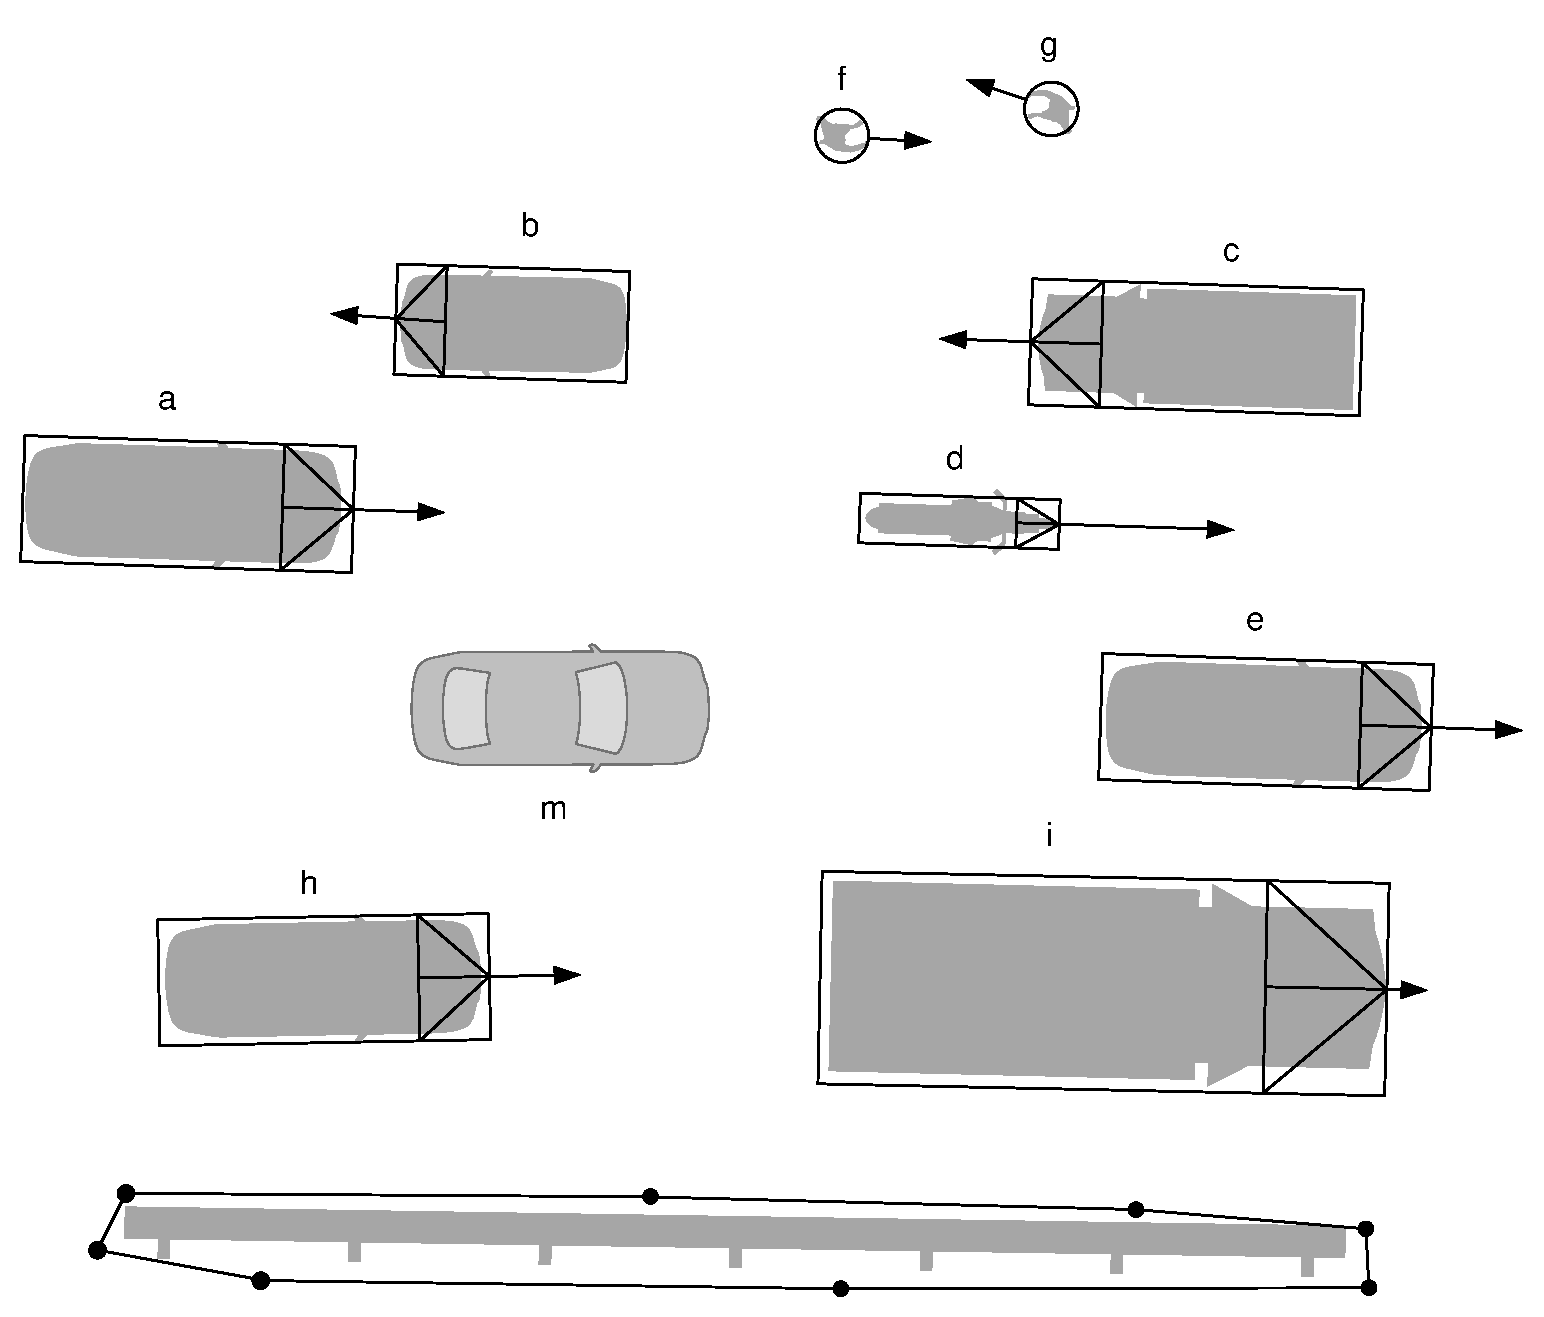
\includegraphics[width=.5\textwidth,clip, trim = 0cm 0cm 0cm 0cm]{2_Objektrepraesentation.eps}
	\hspace{.5cm}
	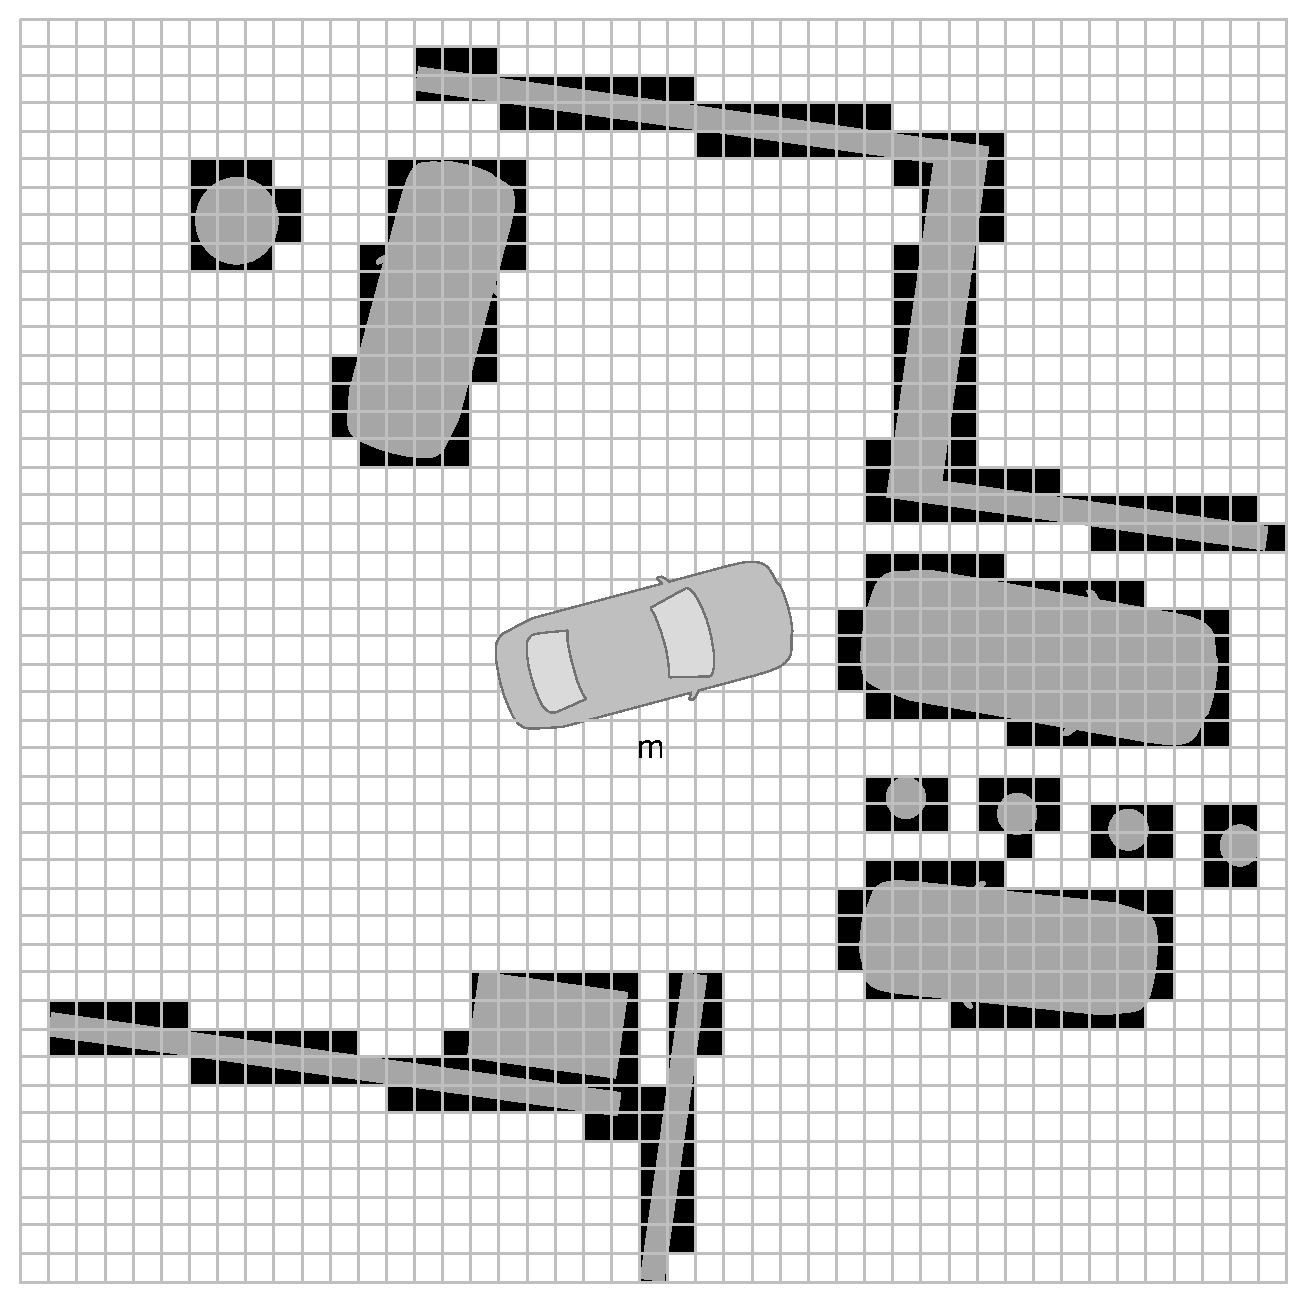
\includegraphics[width=.43\textwidth,clip, trim = 0cm 0cm 0cm 0cm]{2_Belegtheitskarte.eps}
 \caption[Repräsentationsformen des Fahrzeugumfelds]{Repräsentationsformen des dynamischen (links) und statischen (rechts) Fahrzeugumfelds mittels Objektlisten (links) und Belegungskarte (rechts), tatsächliche Objektabmaße in Grau}
 \label{fig:Objektrepraesentation}
\end{figure}

% Existenzwahrscheinlichkeit -> Konfidenzschwelle, Zustandunsicherheiten
% Situationsanalyse
% Fahrzeugumfelderfassung

\subsubsection{Umfeldprädiktion\index{Umfeldprädiktion}} \label{sec:praediction}
Aufgrund der immanenten Dynamik des Verkehrs erfordern aktive Fahreingriffe stets eine Situationsprädiktion. Begreiflicherweise reicht es nicht aus, erst während eines Aufpralls zu bremsen oder zu lenken. Im Vergleich zu den etablierten Methoden der Mehrobjektverfolgung steht jedoch die Entwicklung von Algorithmen zur Situationsprädiktion noch im Anfangsstadium. \\
Eine grobe Einteilung der bestehenden Prädiktionsalgorithmen kann über die Länge des Prädiktionshorizonts erfolgen. Handelt es sich um Prädiktionsverfahren innerhalb eines Sicherheitssystems, das erst kurz vor einer drohenden Kollision aktiv wird (s.\ \abschn{sec:systemactivation}), reicht es aus, die aktuelle Hindernisbewegung zu extrapolieren, z.B. unter der Annahme konstanter Längsbeschleunigungen und Fahrkrümmungen  \cite{Hillenbrand2006, Barth2008}. Soll der Prädiktionshorizont weiter erhöht werden, etwa für eine Assistenzfunktion im Stau, so ist es zielführend, den Verkehrsteilnehmern die Einhaltung der Straßenverkehrsordnung zu unterstellen. In \cite{ferguson2008detection, lawitzkyinteractive} und \citeltex{eichhorn2013Maneuverprediction} wird daher angenommen, dass sich Fahrzeuge langfristig entlang der Spur ausrichten und gleichzeitig so bremsen, dass Auffahrkollisionen vermieden werden. \\
Bei einem noch längeren Horizont (oder aber generell bei Fußgängern) wird häufig von \emph{Intentionserkennung} gesprochen und es überwiegt der stochastische Charakter des Prädiktionsproblems, sodass der zukünftige Aufenthaltsort der Verkehrsteilnehmer nur noch probabilistisch beschrieben werden kann, s.\ \zB \cite{borger2013fahrerintentionserkennung, rohrmuller2008probabilistic, lefevre2012risk, gindele2010probabilistic, althoff2009model, Althoff2010}.\\
Trotz des aktuellen Forschungscharakters ist langfristig, analog zum Umfeldmodell, mit einer zentralen Hindernisprädiktion innerhalb der Fahrzeugarchitektur zu rechnen, die die zukünftige Trajektorie eines jeden Umfeldobjekts permanent schätzt und den Assistenzfunktionen zur Verfügung stellt.



%Stichworte: 
% Umfeldmodell abstraktion: Typ, Abmaße, Position und Dynamikdaten
% Parameter und Zustandsschätzung
% Fehldetektionen und Falschdetektionen
% Bestrebung: Weg von Funktionsspezifischen Algorithmen hin zu einem Umfeldmodell, das bei unterschiedlichen Sensorkonfigurationen für verschiedene Funktionen hergenommen werden kann.
% Verkehrsszene
% Rendundanz bei Senrik bei HAF

 

% Der eigene Fahrzustand muss herangezogen werden um aufgrund der fahrezeugfesten Sensorik auf die Umwelt schließen zu können
\section{Systemaktivierung} \label{sec:systemactivation}
Da das Ein- und Ausschalten von Komfortfunktionen stets dem Fahrer überlassen ist, der abhängig von der Verkehrssituation entscheidet, wann ein System ihm assistieren soll, erfolgt das über eine sog.\ Benutzerschnittstelle \cite{lindberg2012entwicklung}, etwa über einen Knopf. Hierbei ist es dennoch wichtig, die Systemaktivierung und vor allem die -deaktivierung an zusätzliche Bedingungen zu knüpfen, die den technischen Grenzen des jeweiligen Systems Rechnung tragen und eine reibungslose Fahrerübernahme sicherstellen, s.\ \zB \cite{Schaller2008}. \\
Aktive Sicherheitssysteme stehen vor einer ganz anderen Herausforderung. Sie laufen permanent\footnote{Die meisten Sicherheitssysteme können dennoch vom Fahrer deaktiviert werden.} im Hintergrund, da sie ständig die Verkehrssituation  überwachen müssen, um bei gegebenem Anlass sofort mit aktorischen Interventionen zu reagieren. Beim Entwurf der Aktivierungsstrategie besteht nun die Schwierigkeit darin, den Eingriff auf der einen Seite so spät wie möglich vorzunehmen, um den Fahrer nicht ungerechtfertigter Weise zu bevormunden\footnote{Entsprechend der Wiener Straßenverkehrskonvention \cite{UnitedNations1993} gilt: "`\emph{Every driver shall at all times be able to control his vehicle or to guide his animals.}"'}, auf der anderen Seite so früh wie nötig einzuleiten, um eine Kollision zu verhindern. Stehen hierbei dem Assistenzsystem nicht dieselben Eingriffsmöglichkeiten (reduzierte Stellgliedanzahl, verminderter Dynamikumfang der Aktorik) wie dem Fahrer zur Verfügung, kann das in vielen Situationen nur kompromissbehaftet umgesetzt werden \cite{reinisch2012diss,dang2012steering}. Dieser Sachverhalt wird daher auch als sog.\ \emph{Eingriffsdilemma}\index{Eingriffsdilemma} bezeichnet.

Bevor ein kurzer Einblick in die algorithmische Herangehensweise der Aktivierung von Sicherheitssystemen gegeben wird, sei auf die Norm ISO 26262 \cite{ISO26262} hingewiesen, die allgemeine Entwicklungsmethoden der Funktionalen Sicherheit definiert  \cite{hillenbrand2011funktionale}. Sie stellt den Stand der Technik bei der Absicherung von sicherheitsrelevanten elektrischen/elektronischen Systemen in Kraftfahrzeugen dar und ist damit verbindlich vom Entwicklungsingenieur bei der Planung, Entwicklungsdurchführung und Validierung von Serienfahrerassistenzsystemen anzuwenden. Im Idealfall findet sie allerdings bereits im Forschungsstadium Berücksichtigung, da dann ein reibungsloser Ergebnistransfer in Richtung Serienentwicklung gewährleistet ist. \\
Zur Minimierung des verbleibenden Restrisikos (hier der aktivierten Assistenzfunktion) fordert die Norm unter anderem eine Sicherheitsintegrität des Systems, welche über sog.\ \emph{Automotive Safety Integrity Levels}\index{Automotive Safety Integrity Level} (ASIL) bewertet wird. Sie berechnen sich aus dem Schweregrad einer möglichen Verletzung, der Beherrschbarkeit der Fehlfunktion durch den Fahrer und der Häufigkeit der relevanten Fahrsituation. Je nach ASIL-Einstufung (A bis D) ergeben sich dann Konsequenzen für beispielsweise das Redundanzkonzept\index{Redundanz}, die formale Verifikation, die Selbstdiagnosefähigkeit, die Toleranzen oder die Komponententests des Assistenzsystems.

\subsection{Zustände einer unvermeidlichen Kollision} \label{sec:ics}
Die mobile Robotik beschäftigt sich seit jeher mit Algorithmen der Bewegungsplanung inmitten von Hindernissen, s.\ beispielsweise \cite{latombe1990robot, lavalle2006pa, fox1997dynamic, Fiorini1998}. Mit Hilfe sog.\ \emph{Konfigurationsraum}-Hindernisse\index{Konfigurationsraum} (kurz $\mathcal{C}$-Hindernisse) wird hierbei das Planungsproblem dahingehend vereinfacht, dass in den Hindernissen bereits die Abmaße des mobilen Roboters Berücksichtigung finden und der Roboter selbst auf einen Punkt reduziert werden kann. Für eine statische\footnote{Aufgrund der vereinfachten Repräsentation der beweglichen Hindernisse, etwa durch Rechtecke, ist es effizienter \cite{zieglerfastcollision2010, Lin1998}, die Kollisionsfreiheit einer konkreten Trajektorie innerhalb des Optimierungsalgorithmus hierarchisch abzuprüfen, anstelle die Konfigurationshindernisse für jeden Zeitschritt des Optimierungshorizonts komplett zu berechnen.} Umgebung erfolgt die Berechnung dieser $\mathcal{C}$-Hindernisse durch Einsatz von modernen Grafikkarten im Millisekundenbereich \cite{Tanzmeister2014ConfSpaceCosts}, wovon die in den Kap.\,\ref{chap:dynamische_Optimierung_dynamisch}, \ref{chap:dynamische_Optimierung_direkt} und \ref{chap:dynamische_Optimierung_indirekt} vorgestellten Algorithmen rechenzeittechnisch erheblich profitieren. \\
Die sog.\ Zustände einer unvermeidlichen Kollision \cite{fraichard2007short} (\emph{Inevitable Collision States}\index{Inevitable Collision States}, ICS), stellen gewissermaßen die Erweiterung der $\mathcal{C}$-Hindernisse dar. Sie beinhalten nämlich nicht nur die Geometrie des mobilen Roboters, sondern auch dessen \emph{zukünftige Modelldynamik}. Ein Robotik-System befindet sich nämlich genau dann in einem ICS, wenn, ganz gleich welche zukünftige Systemtrajektorie eingeschlagen wird, das System unweigerlich mit einem der Hindernisse kollidiert. \\
Für die Trajektorienplanung inmitten statischer und dynamischer Hindernisse bietet das ICS-Konzept einen ganz erheblichen Vorteil: Existiert eine effiziente ICS-Berechnung (ein sog.\ ICS-\emph{checker} \cite{martinez2009collision}), so reicht es für die Berechnung sicherer Trajektorien aus, vereinfacht gesprochen, die Überprüfung auf Kollisionen mit Hindernissen auf einem endlichen Horizont durchzuführen, wenn sichergestellt wird, dass der Trajektorien-Endpunkt nicht in einem ICS liegt \cite{fraichard2007short}, s.\ später Abschn.\,\ref{sec:stab_mpc}.
Aufgrund des erheblichen Rechenaufwands bei einer numerischen ICS-Berechnung, s.\ beispielsweise \cite{Lawitzky2014ICRA, falcone2011predictiveassessment, Karrenberg2008},  %aoude2010Threat, 
werden für die Fahrerassistenz stark vereinfachte Fahrzeugmodelle eingesetzt. So kann ein reines Bremsmanöver mittels Doppelintegrator mit beschränktem Eingang approximiert werden, wofür die 
ICS-Menge, wie in \abb{fig:ausweichen_vs_bremsen} dargestellt, analytisch berechnet werden kann. Soll zusätzlich die Querbewegung hinzugezogen werden, bietet sich die Approximation der Fahrzeugdynamik durch den sog.\ Kamm'schen Kreis\index{Kamm'scher Kreis} \cite{breuer20012bremsenhandbuch} an, s.\ \abb{fig:Beschleunigungskreise}.

%ICS kann herangezogen um Notbremsung auszulösen, und ausweichen zu planen (am Ende wieder in einem ICS) \cite{fraichard2007short}.
%	- Erweiterung des Dynamic Window Ansatzes
%	- ICS: Halber Tacho als Fußnote
%	ICS langfristig für HAF interessant: Erfassungshorizont endlich
	
%	- Berechnungsmethoden:
%	- Erreichbarkeitsmengen (mit Garantien)
%	- Monte-Carlo Simulationen
%	- Rückwärtsrechnen vom HIndernis
%	- Trajektorienplanung kann auch bei der Eingriffsstrategie helfen.
	
%	\cite{Althoff2010} % Diss

%\cite{falcone2011predictiveassessment} % Invarianten Mengen Volve invariant set theory von NMPC

%\cite{anderson2010optimal} % nmpc threat assesment


%\cite{Lawitzky2014ICRA}

%\cite{aoude2010Threat} % intersections Erreichbarkeitsmengen

%\cite{anderson2012constraint} % Hauptsächlich aktivierung mit minimalinvasiven manövern

\begin{figure}[h]
\centering
	\psfrag{I}[cc][cc]{ICS$_\text{Bremsen}$}
	\psfrag{J}[cc][cc]{ICS$_\text{Lenken}$}
	\psfrag{w}[tr][tr]{$\sqrt{-2 x a_\text{max}}$}
	\psfrag{u}[tr][tr]{$-x \sqrt{\frac{a_\text{max}}{2b}}$}
	\psfrag{h}[br][br]{Hindernis (0,0)}
	\psfrag{1}[cr][cr]{$v$}
	\psfrag{2}[tl][tl]{$x$}
	\psfrag{0}[cl][cl]{$v_c$}
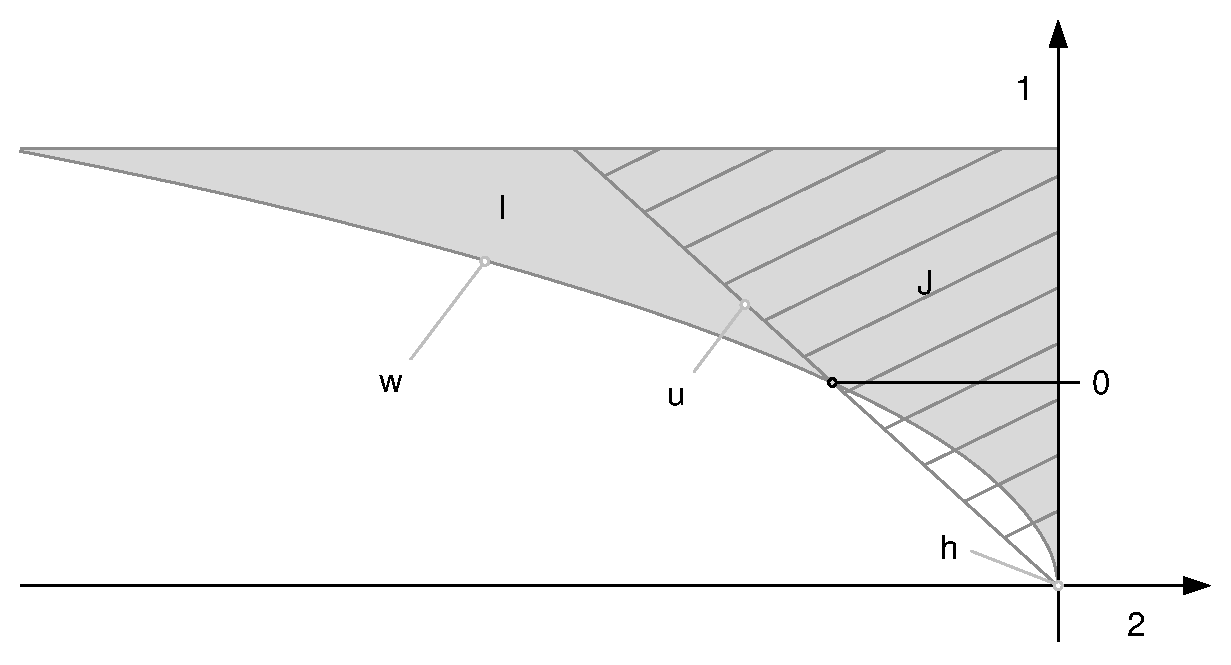
\includegraphics[width=.9\textwidth,clip, trim = 0cm 0cm 0cm 0cm]{2_1d_ICS.eps}
\caption[Zustandsmenge einer unvermeidlichen Kollision durch Bremsen]{Zustandsmenge einer unvermeidlichen Kollision durch Bremsen (ICS$_\text{Bremsen}$, grau) des Systems $\dot x = v$; $\dot v = u \in [-a_\text{max}, a_\text{max}]$ zur Darstellung einer Auffahrsituation auf ein punktförmiges Hindernis im Ursprung; Im Vergleich dazu die (projizierte) Zustandsmenge einer unvermeidlichen Kollision durch konstante Querbeschleunigung (ICS$_\text{Lenken}$, schraffiert, Hindernisüberlappung $b$); Für Geschwindigkeiten unterhalb von $v_c$ kann bei Annäherung an das Hindernis zur Kollisionsvermeidung noch länger gebremst als ausgewichen werden, oberhalb von $v_c$ gerade umgekehrt, vgl.\ \cite{reinisch2012diss, schmidt2014fahrstrategien}.}
 \label{fig:ausweichen_vs_bremsen}
\end{figure}

		
		
\subsection{Subjektive Kritikalitätsbewertung\index{Kritikalitätsbewertung} des Fahrers} \label{sec:ttc} %empirisch
In den aktuellen Notbremsseriensystemen wird nicht erst dann gebremst, wenn eine Kollision unvermeidbar ist \cite{reinisch2012diss} und sich das Fahrzeug demnach in einem ICS befindet. Der Bestimmung des Eingriffszeitpunkts liegt nämlich eine andere, weniger konservative Überlegung zugrunde, die als Lösung eines Klassifikationsproblems angesehen werden kann. Aufgabe des Assistenzsystems ist demnach zu erkennen, ob der Fahrer überhaupt den potentiellen Kollisionspartner wahrgenommen hat oder nicht, und das möglichst früh. 
Da sich eine kamerabasierte Fahrerüberwachung bis dato nicht im Serieneinsatz befindet, % (s.\ auch \abschn{sec:grundlagen_bewertung}) 
müssen hierfür die Bremssysteme auf Basis der Relativbewegung zum Hindernis entscheiden, ob ein gewolltes Manöver oder ein Fahrfehler vorliegt. Als Bemessungsgrundlage (Klassifikationsmerkmal) hat sich vor allem die sog.\ \emph{time-to-collision}\index{time-to-collision}, kurz TTC, bewährt, welche die Zeit darstellt, die unter Beibehaltung der relativen Bewegungsdynamik zwischen den Kollisionspartnern bis zum Aufprall verbleibt. Sie repräsentiert nachweislich die vom Fahrer subjektiv wahrgenommene Kritikalität eines Auffahrmanövers. \\
Auch wenn die TTC ein breites Spektrum an Auffahrsituationen abdeckt, so berücksichtigt sie nicht die relative Position und Bewegung der Kollisionspartner quer zur Fahrtrichtung. So kann bei einer geringen Querüberlappung mit dem Hindernis der vermeintlichen Kollision durch eine minimale Lenkbewegung mühelos entgangen werden und das Manöver damit vom Fahrer gewollt sein. Um dies mit zu berücksichtigen, bietet sich als weiteres Kritikalitätsmaß die sog.\ \emph{time-to-steer}\index{time-to-steer} (TTS) an, also die Zeit, die verbleibt, bis der Fahrer durch Lenken spätmöglichst dem Unfall entgehen kann. Analog dazu definiert sich die \emph{time-to-brake}\index{time-to-brake} (TTB) oder kombiniert die \emph{time-to-react}\index{time-to-react} (TTR) \cite{Hillenbrand2006}. \\
In Bezug auf \abschn{sec:ics} stellt damit die TTC die zeitliche Distanz zu einem $\mathcal{C}$-Hindernis dar. Die TTR wiederum beschreibt nichts weiter als die verbleibende Zeit, bis sich das Fahrzeug in einem ICS befindet.



% - TTC: Warndilemma, da Reaktionszeit des Fahrers --> Aktive Eingriffe haben dieses Problem nicht. Ganz zu schweigen davon, dass der Fahrer die Warnung auch richtig interpretieren muss.

% Konfigurationsraum: berücksichtigt keine dynamik (alle Systemzustände) sondern nur position und Ausrichtung

% Ersatz für ICS: alle Zustände in denen ein Fahrer im Normalen fahrbetrieb sich nicht aufhält. KRitikalität

%Bremsen ist grndsätzlich sicherer als Ausweichen, weil Energie abgebaut wird.

%footnote: StvO ist so ausgelegt, dass immer einer vorfahrt hat und der andere gewähren muss: damit entsteht nich: Er denkt, dass ich denke, dass er denkt.
%Rückwirkungen des eigenen Fahrzeugs auf andere: Zumutbare verzögerungen in der Serie

%ICS liefern ein gutes Framework bestehende Assistenzsysteme und deren Auslösung zu interpretieren, neue Auslösekriterien zu erarbeiten und Trajektorienplanung für HAF sicherer zu gestalten.
		
	
		% Kreismethode
\begin{figure}[h]
	\psfrag{H}[cc][c][1.0]{Hindernis}
	\psfrag{a}[lb][lb][1.0]{$a_\text{max}t^2$}
	\psfrag{v}[tc][tc][1.0]{$v_0 \Delta t$}
\centering
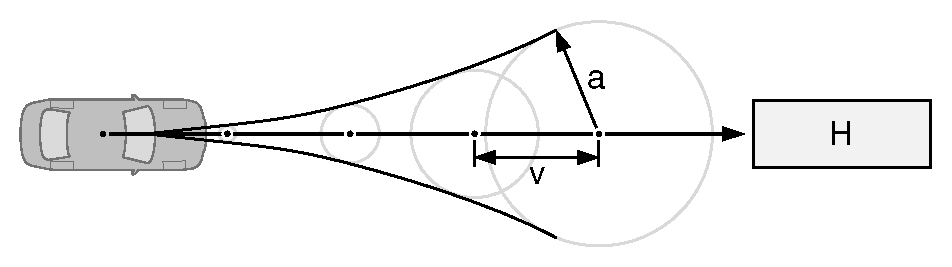
\includegraphics[width=1\textwidth,clip, trim = 0cm 0cm 0cm 0cm]{2_Beschleunigungskreise.eps}
 \caption[Erreichbare Schwerpunktpositionen]{Erreichbare Schwerpunktpositionen der durch maximale Beschleunigungen $a_\text{max}$ approximierten Fahrzeugdynamik \cite{schmidt2014fahrstrategien} (Kamm'scher Kreis \cite{breuer20012bremsenhandbuch}); Wie dem diagonalen Beschleunigungspfeil entnommen werden kann, beinhaltet die Erreichbarkeitsgrenze (schwarze Linie) beim Ausweichen immer auch eine Verzögerungskomponente, die jedoch in der Praxis häufig vernachlässigt wird.}
 \label{fig:Beschleunigungskreise}
\end{figure} 



% Abschätzungen über Physikalische Extrema: Kammscher Kreis

% Begriff: Deeskallationsmanöver


% Auslösung muss immer Wechselwirkungen berücksichtigen, wenn auch vereinfacht: Rückwärtiger Verkehr: zumutbare Verzögerung

% TTC kann auf als Merkmal für Lernende Verfahren sein.
% TTC verwendet Modell: z.B. konst. Geschwind., konst. Beschleun. etc.

% TTC: empirisch der Zusammenhang zur subjektiven Kritikalität

% Im Gegensatz dazu modelliert fTTR die physikalische Kritikalität; mit fTTR = 0 liegt z.B. der letztmögliche Zeitpunkt einer Deeskalation vor.

% neue algorithmen: Zeitliche Abfolge der Daten

% Althoff: Erreichbarkeitsanalyse


% Beispielbild: Berücksichtigung des Fahrbahnverlauf vs. geradeausfahren


% Fahrerinitiierte Systeme: Bremsassistent oder Ausweichassistent
% Automatisierte Eingriffe: Hohes Risiko

% TTC, TTR, TTB, TTS

% Physikalische Extrapolation (keine Prädiktion)

% rudimentär Prädiktion

% Fahrerüberwachung

% Unberechtigte Eingriffe, sog. Falschauslösungen (sportliche Fahrweise, Akzeptanz) müssen ebenso wie Fehlauslösungen vermieden werden.

% Fahrerreaktion muss berücksichtig werden -> Diss Reinisch

% Prädiktion anhand vorheriger Beobachtungen zu schätzen + Karte

% Unterscheidung: auf Manöverebene: Einscherer oder nicht, Abbieger etc.
% oder auf Trajektorienebene

% Einfachster Fall: TTC + Überlappung

% Algorithmik: Klassifikationsproblem

% Ausweichen vs. Bremsen: Eingriffsdillemma
% Falls auch autom. ausgewichen werden soll: Hindernis in der Fahrzeugmitte: Welche Richtung?
% Zusätzliche Probleme beim Ausweichen: Es muss auch wirklich frei sein. Bremsen macht immer das Richtige
% Kurzfristige Prädiktion: Es reicht sich auf die Physik zu verlassen: Es kann ja auch ein Fehler eines anderen Verkehrsteilnehmer vorliegen, sodass dieser selbst ein ander Fahrzeug rammt.
% Langfristige Situationsprädiktion muss wechselwirkungen zwischen den Verkehrsteilnehmern berücksichtigen

% Volvopaper: Welche Möglichkeiten hat der Fahrer?
% Inevitable Collision states

% Agentenbasierte Systeme?

% Methode sollte so schnell sein, dass sie auch zur Trajektorienplanung eingesetzt wird --> konstruktiv

% Monte Carolo simulationen

% Einhüllende

% Diskrete stochastische Systeme: Modellierung mittels Markov-Ketten

% Fahrer: hybrides system: Zustansübergänge mit kontinuierlichem Dynamik

% Stochastische Verifikationsmethoden

% Deterministishe Verifikation

% Kooperatives Umfeld (wird unterstellt), Verkehrsregeln geben die Abhängigkeit der reaktion zwischen den Hindernissen vor: Schwierigkeit: wie werden fehler erkannt?

% Modellierung: Gesamtverkehr stellt Systemzustand dar, der durch die Stellgrößen beeinflusst werden kann. Falls andere Fahrzeuge auf uns reagieren, dann sind auch ihr Trajektorien beeinflussbar. In manchen Situationen muss dies vorausgesetzt werden, da sonst eine Bremsung auf den vordermann eine kollision mit dem HIntermann zur folge hätte.

%\section{Optimierungskriterien und Koordinatenwahl}
%\subsection{Kartesische Koordinaten}
%\subsection{Frenet-Koordinaten}
%% Pfad vs. Trajektorie
%% Koordinatenwahl [XY, Frenet (Linearisierung um Traj.)]

\section{Bewertung} \label{sec:grundlagen_bewertung}
Die Beschreibung der Problemstellung aktiver Fahreingriffe des vorliegenden Kapitels erfolgt in zwei Teilen.
Der erste Teil leitet die interne Struktur eines Fahrerassistenzsystems her. Motiviert durch die beobachtbare Fahrweise routinierter Fahrzeugführer während hochdynamischer Manöver wird das klassische Drei-Ebenen-Modell derart modifiziert, dass es mit gesteigerter Fahrzeugbeherrschung einen immer größeren Teil des Fahrzustands auf der Führungsebene berücksichtigt. Die dort permanent zu lösende Aufgabe wird regelungstechnisch als Optimalsteuerungsproblem interpretiert, wodurch ein modellprädiktiver Regelkreis entsteht, der für die Stabilisierung des rückgeführten Teilfahrzustands zuständig ist. Die den Optimalsteuerungsproblemen zugrunde gelegten Optimierungskriterien berücksichtigen hierbei den Komfort, die Sicherheit und die Effizienz mit von Fahrer zu Fahrer unterschiedlichen Wichtungsfaktoren. \\
Die anschließende sog.\ Stabilisierungsebene wiederum wird als unterlagerter Regler betrachtet, wodurch im Zusammenspiel mit der modellprädiktiven Regelung ein kaskadierter Regelkreis entsteht, der auf der überlagerten Ebene den Optimierungskriterien des Manövers Rechnung trägt und auf der unterlagerten Ebene die spezifischen Eigenschaften des Fahrzeugs berücksichtigt.
%Neben den Standardsituationen wie Spur- und Abstandhalten erklärt der gegenüber dem Standardmodell modifizierten Systemaufbau auch die Unterstützung des Fahrers in Notfallsituationen ermöglicht, für welche eine permanente Optimierung des Fahreingriffs entsprechend der verfügbaren Fahrzeugdynamik und Umfeldinformation unabdingbar ist.

Zur Erleichterung der Übertragung des neuen Fahrermodells auf Fahrerassistenzsysteme und zur einheitlichen Betrachtung bestehender Algorithmen werden anschließend aus regelungstechnischer und robotischer Sicht die Begriffe \emph{Trajektorien-} und \emph{Bahnplanung}, \emph{Optimalsteuerung} sowie \emph{Optimale} und \emph{Modellprädiktive Regelung} erklärt und verglichen. 

Nach Darlegung der internen Grundstruktur einer Fahrerassistenz der Führungsebene, fokussiert der zweite Teil auf die dem System zur Verfügung stehenden Ein- und Ausgangsgrößen. Hierbei wird erkennbar, dass aus Entwicklersicht moderne Fahrzeuge im Hinblick auf die Möglichkeiten, die Fahrdynamik aktiv zu beeinflussen, kaum noch Wünsche offen lassen. Während zur Erprobung hochautomatisierten Fahrens noch vor einigen Jahren aufwändig Zusatzaktorik in die Versuchsträger eingebaut werden musste \cite{werivframe08, rauskolb2008caroline}, so reicht heute die Manipulation der Software des zuständigen Seriensteuergeräts aus, damit Lenkung, Gas und Bremse von extern angesprochen werden können. Mehr noch: Aufgrund der durchdachten Fahrzeugarchitektur stehen die detaillierten %in \abschn{sec:aktuatorik} 
Aktorikschnittstellen, namentlich das Sollhandmoment oder der -lenkradwinkel sowie das Antriebs- oder Bremsmoment am Rad, transparent zur Verfügung. Damit können die Fahrerassistenzfunktionen weitgehend unabhängig von der technischen Umsetzung der Stelleingriffe im jeweiligen Fahrzeug entworfen und leichter koordiniert werden, was den Entwicklungsprozess enorm beschleunigt und die Entwicklungskosten reduziert. \\
Dasselbe gilt für die zentrale Auswertung und Bereitstellung der erfassten Sensorinformationen. Auch wenn in aktuellen Serienfahrzeugen bestimmte Messgrößen wie die Gierrate (unnötiger Weise aus technischer Sicht) an mehreren Stellen im Fahrzeug von verschiedenen Teilsystemen erfasst werden, so lassen moderne Forschungsfahrzeuge %\cite{BMW_Autobahn, Daimler} 
eine klare Tendenz zu einer zentralen Informationsverarbeitung erkennen. Als Beispiel profitieren von einer verbesserten Schwimmwinkelschätzung dann zukünftig nicht nur das Elektronische Stabilitätsprogramm, sondern auf einen Schlag auch die Eigenlokalisierung, die Trajektorienberechnung, die Fahrzeugquerführung, die Mehrobjektverfolgung und die Situationsprädiktion. \\

Rückblickend auf den Wettkampf DARPA Urban Challenge 2007 kann aus heutiger Sicht festgehalten werden, dass ein Großteil der Kritik an den damaligen Ansätzen, s.\ \zB \cite{urmson2008adu, montemerlo2008junior, bacha2008odin, jfr2008}, ungerechtfertigt war. Hierzu zählt die Verwendung von Karteninformation, was unmittelbar mit der Abhängigkeit des Systems von einer entsprechend genauen Eigenlokalisierung verbunden ist (s.\ \abschn{sec:globalelok}). Nach heutigem Kenntnisstand ist nämlich eine Karte auf absehbare Zeit unverzichtbar, wenn es um die Realisierung einer Großzahl neuer Sicherheits- und Komfortfunktionen geht, sodass eisern an einer serientauglichen Eigenlokalisierung gearbeitet wird (s.\ ebenfalls \abschn{sec:globalelok}). Ein weiterer Kritikpunkt stellte die teils über mehrere Ebenen auf dem Dach angeordnete Rundumsensorik dar, die im Hinblick sowohl auf die Kosten als auch auf die Fahrzeugoptik aus Kundensicht inakzeptabel ist. Im Vergleich dazu unterscheiden sich aufgrund der unauffälligen Integration der Sensorhardware die heutigen Forschungsfahrzeuge der Hersteller von außen kaum noch von Serienfahrzeugen, bei teils gesteigerter Informationsgenauigkeit. Der Kostenaspekt einer umfangreichen Rundumsensorik bleibt jedoch, wie so häufig in der wettbewerbsgeprägten Automobilbranche, nach wie vor ein heikles Thema. Letztendlich entscheidet er darüber, ob sich ein Assistenzsystem langfristig rechnet.



%Dennoch hilft ein Grundverständis für die Funktionsweise der Einzelkomponenten, der Überlagerung mit dem Fahrer sowie deren Regelung bei der Modellierung und dem modellbasierten Reglerentwurf im Fahrerassistenzsystem, s.\ Kap.\,\ref{chap:stabilisierung}. 
% Fahrerüberwachung ganz wichtig für Vision zero
% c2x
% Rundumsensorik top
% Komfortfunktionen und Sicherheitsfunktionen nutzen dieselbe Sensorik
% Nachfolgende Kapitel: Gibt dem Entwickler für diese Aufgabe einen systematisierten Überblick über Methoden der Fahrzeugstabilisierung und Trajektorienoptimierung. Vorteilhafte Aufteilung in Regelung und Planung, Formulierung des Optimierungsproblems, Lösungsmethoden

%Aufteilung in bestehende/bewährte Stabilisierungsmethoden (ABS, DSC)

Zusammenfassend stehen damit aus Sicht der aktuellen Fahrerassistenzentwicklung von aktiven Fahreingriffen folgende drei Fragenstellungen im Mittelpunkt: 
\begin{itemize}
\item Welche nutzbringenden Sicherheits- oder Komfortfunktionen lassen sich auf Basis der bestehenden Aktorikschnittstellen mit der verfügbaren Sensorinformation umsetzen?
\item Welche Minimalanforderungen ergeben sich hierbei aus der anvisierten Fahrerassistenzfunktion an das Sensoriksetup?
\item In welche Richtung müssen Aktorik und Sensorik weiterentwickelt werden, um die angestrebte Funktionsqualität und -zuverlässigkeit zu realisieren?
\end{itemize}
An dieser Stelle sei an den kreativen Ingenieur und seine Arbeitsgruppe appelliert, neue Fahrerassistenzfunktionen nicht im Labor zu entwickeln. Vielmehr ist es zielführend, wenn der Forscher und Entwickler täglich mit offenen Augen in sein Fahrzeug steigt und sich dabei in die Lage unterschiedlicher Kunden versetzt. So kann aus einer erlebten Fahrsituation eine erste Funktionsidee entstehen, die in mehreren algorithmischen Iterationszyklen und Prototypen zu einer wertigen Assistenzfunktion heranreift. \\
Kreativität beruht jedoch zu großen Teilen auf Können. Auf es zielen die nachfolgenden Kapitel ab, indem methodisches Wissen in systematisierter Form vermittelt wird, welches sich, belegt anhand zahlreicher Literatur, in der Entwicklungspraxis aktiver Fahreingriffe als unverzichtbar herausgestellt hat. Die Kapitelinhalte beschränken sich insbesondere nicht auf die Darlegung der bloßen Theorie, sondern legen besonderen Wert auf die beispielhafte Beschreibung praktischer Umsetzungen. Somit wird der Leser befähigt, Parallelen zu neuen Fahrerassistenzfunktionen zu ziehen, damit er sie in vorteilhafter Weise mathematisch formulieren kann, um sie anschließend algorithmisch zu lösen und schließlich praktisch umzusetzen und zu erproben.

\cleardoublepage


% Zusammenfassung und Ausblick auf weiter Kapitel, s. z.B. Mikut Seite 237

%\begin{figure}[H]
	%\psfrag{0}[c][c][1.0]{$t_0$}
	%\psfrag{1}[c][c][1.0]{$t_1=t_0+\delta$}
	%\psfrag{2}[c][c][1.0]{$t_c=t_0+T_c$}
	%\psfrag{3}[c][c][1.0]{$t_p=t_0+T_p$}
	%\psfrag{4}[c][c][1.0]{Kontrollhorizont $T_c$}
	%\psfrag{5}[c][c][1.0]{Prädiktionshorizont $T_p$}
	%\psfrag{6}[c][c][1.0]{Vergangenheit}
	%\psfrag{7}[c][c][1.0]{\textbf{Prädiktion}}
  %\psfrag{a}[c][b][1.0]{Systemzustand x}
	%\psfrag{b}[c][c][1.0]{prädizierter Systemzustand $\bar{x}$}
	%\psfrag{c}[c][b][1.0]{Stellgröße u}
	%\psfrag{d}[c][b][1.0]{zu optimierende Stellgröße $\bar{u}$}
	%\centering
  	%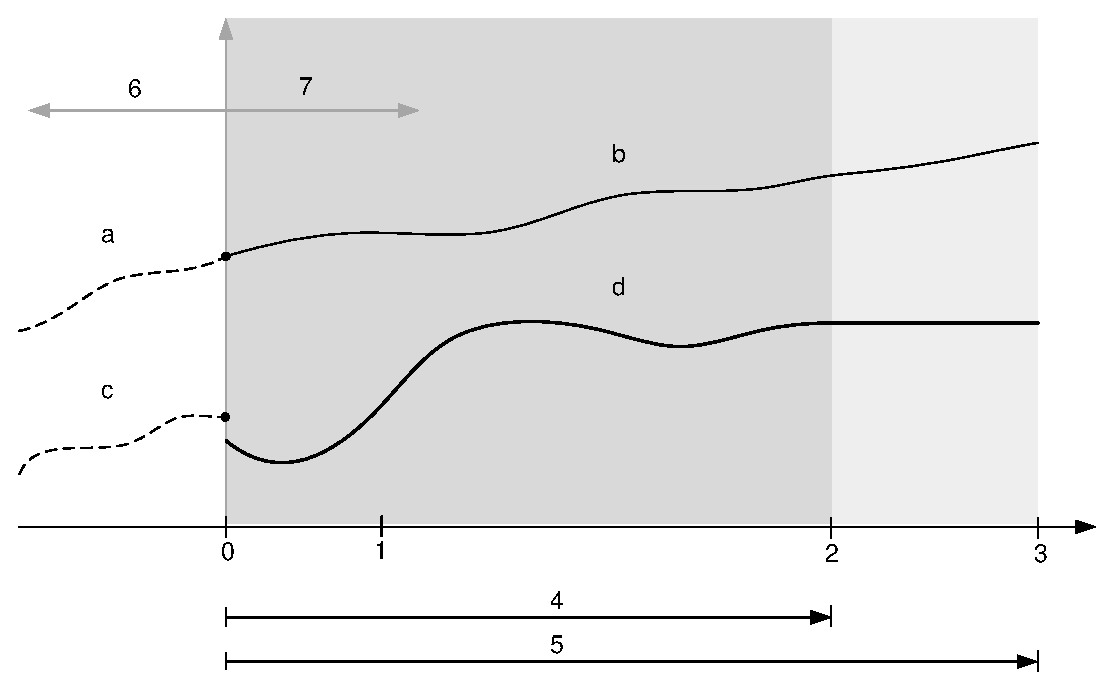
\includegraphics[width=1\textwidth,clip, trim = 0cm 0cm 0cm 0cm]{2_mpc_grundidee.eps}
		%\vspace{-0.1cm}
  	%\caption[Grundidee der modellprädiktiven Regelung]{Grundidee der modellprädiktiven Regelung, abgewandelte Darstellung nach \cite{Findeisen2002}}
    %\label{fig:grundidee_nmpc}
		%\vspace{-0.2cm}
%\end{figure} 

%\begin{figure}[H]
%\hspace{-0.9cm}
%\vspace{0.1cm}
	%\psfrag{1}[c][c][0.97]{\parbox[c]{7cm}{\begin{center}Lösungverfahren für die MPC\vspace{-0.08cm}\\ in der Optimalsteuerungsformulierung\end{center}}}
	%\psfrag{2}[c][c][0.97]{\parbox[c]{7cm}{\begin{center}Dynamische\vspace{-0.08cm}\\ Programmierung:\\\textit{\footnotesize Hamilton-Jacobi-Bellman-Gl.}\end{center}}}
	%%\psfrag{2}[c][c][0.97]{\parbox[c]{7cm}{\begin{center}Dynamische\vspace{-0.08cm}\\ Programmierung:\vspace{0.15cm}\\\textit{\footnotesize Hamilton-Jacobi-Bellman-Gl.\vspace{-0.15cm}\\ (Lockup-Table für Zustandsraum)}\end{center}}}
	%\psfrag{3}[c][c][0.97]{\parbox[c]{7cm}{\begin{center}Indirekte Methoden:\vspace{-0.08cm}\\ Minimumsprinzip von Pontryagin\\ \textit{\footnotesize Lösung mittels Variationsrechnung}\end{center}}}
	%\psfrag{4}[c][c][0.97]{\parbox[c]{7cm}{\begin{center}Direkte Methode:\vspace{-0.08cm}\\ Parametrisierung des Lösungsraums\vspace{0.15cm}\\ \textit{\normalsize\footnotesize Transformation in endlichdimensionales\vspace{-0.15cm} \\nichtlineares Optimierungsproblem}\end{center}}}
 %\psfrag{5}[c][c][0.97]{\parbox[c]{7cm}{\begin{center}Single Shooting\vspace{0.05cm}\\ \textit{\footnotesize Diskretisiert Steuervariablen\vspace{-0.15cm} \\(sequentiell)}\end{center}}}
 %\psfrag{6}[c][c][0.97]{\parbox[c]{7cm}{\begin{center}Kollokation\vspace{0.05cm}\\ \textit{\footnotesize Diskretisiert Steuer-\vspace{-0.05cm}\\ und Zustandsvariablen\vspace{-0.15cm} \\(simultan)}\end{center}}} 
 %\psfrag{7}[c][c][0.97]{\parbox[c]{7cm}{\begin{center}\vspace{0.05cm}Multi Shooting\vspace{0.05cm} \\ \textit{\footnotesize Diskretisiert Steuervariablen\vspace{-0.05cm} \\ und führt künstliche\vspace{-0.05cm} \\Zustandsvariablen ein\vspace{-0.15cm}\\ (simultan)}\end{center}}}
	%%\centering
		%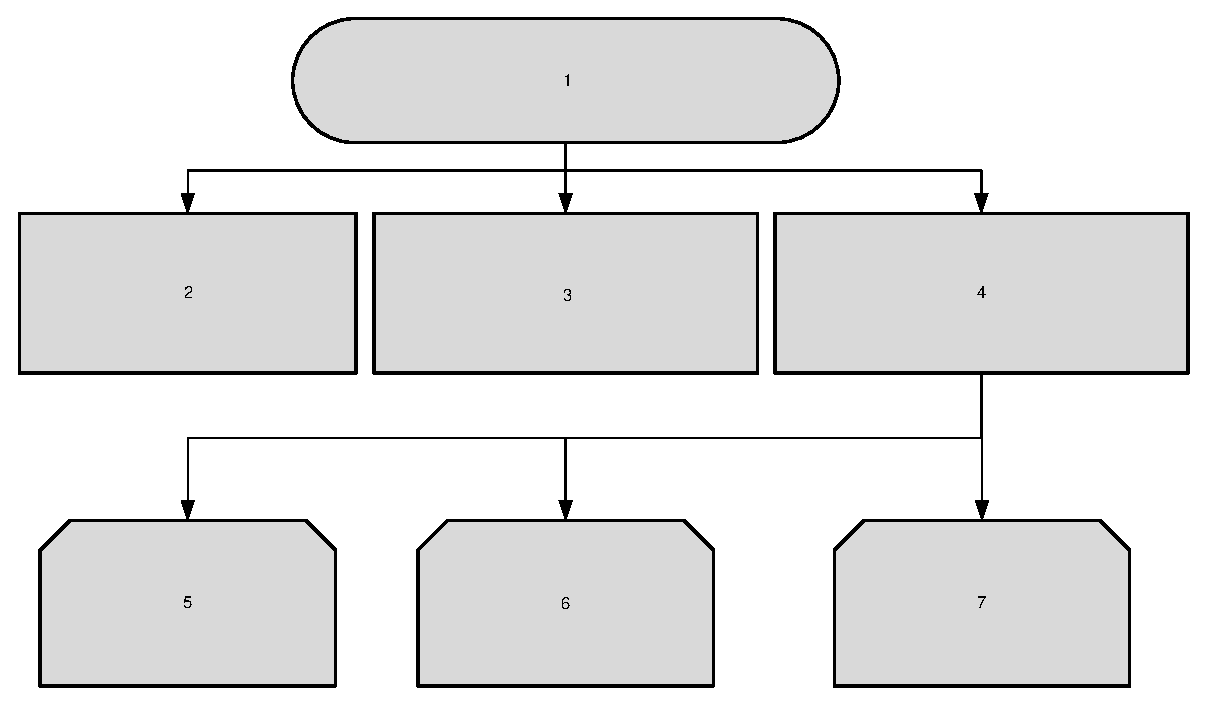
\includegraphics[width=1.11\textwidth,clip, trim = 0cm 0cm 0cm 0cm]{1_optimalsteuerung_uebersicht.eps}
	%\vspace{0.001cm}
	%\caption[Übersicht über die verschiedenen Zugänge zu Optimalsteuerungsproblemen]{Übersicht über die verschiedenen Zugänge zu Optimalsteuerungsproblemen,\\ abgewandelte Darstellung nach \cite{diehl_fast_multipleshooting}}
	%\label{fig:optimalsteuerung_uebersicht}
%\end{figure}



% Zustandsautomaten? Ist prinzipiell wichtig, da Teil eines jeden FAS
% Optimierung offline -> LUT
%	\section{Allgemeine Vorgehensweise}
% Best practice
% Iterativer prozess: modellierung evaluation, anpassung der modelle, nachhaltigkeit der entwicklung, viel simulation, modelle anwendung s abhängig, systemverständnis
% Binsenweisheiten, die nicht häufig genug wiederholt werden können, da sie immer noch falsch gemacht werden.
% Statischer, dynamischer Fahrsimulator
%	\subsection{Simulation}
%	\subsection{Fahrversuche}
	% 
%	\subsection{Absicherung}

% Hands-on-detection, Bewusst funktion schlechter machen um Missbrauch zu verhindern
% Probandenstudien, Expertentests

% Rausgeschmissen:
% % ISO 26262, Asil etc.
% Simulation, Fahrversuch, Prototypenbau, Probanden, Absicherung
% Aufbau eines Fahrerassistenzsystems

%	Entwicklungskriterien
% ZEISS-Punkte herein
% Statistische Auswertungen
% Nutzerakzeptanz
% Packaging (Angebotspakete)
% Cost Engeneering
% Diskretisierungsmethoden, Verweis auf folgende Kapitel


% TODO: Formulierung als OCP anstelle MPC in anschließenden Kapiteln erwähnen
% Story:
% Trajektorienplanung -> OSP
% Allg. Formulierung OSP
% Fahrzeugspez. Formulierung OSP
% Ausblick auf Lösungsmethodik:
% - Modifikation der Problemstellung bei DP und DM
% OS -> Rückkopplung -> Stabilitätsbetrachtungen
% Stabilität v. Lyapunov -> Lyapunovfunktion
% Stabilität von MPC, unendlicher, quasiunendlicher Opt.-Horizont
% Robustheitssteigerung druch unterl. Regelung
%  - ...
%  - Praxiserprobte unterlagerte Regler
% Beispiel Gespann
% Ausblick auf nachfolgende Kapitel zur OSP
\chapter{Stabilität und Robustheit optimaler Fahrmanöver}\label{chap:stabilisierung}
\zitat{If everything is under control \\
you are just not driving fast enough.}{Sir Stirling Moss}


Aufgrund der theoretisch unendlich vielen Möglichkeiten bei der Planung einer Fahrtrajektorie muss eine Bewertung in einem bestimmten Sinne vorgenommen werden, um die \emph{beste} Trajektorie wählen zu können. Diese Herangehensweise wird als Optimierung bezeichnet. Wie hierzu in \cite{foellingeroptimal} angemerkt wurde, wird jedoch im gängigen Sprachgebrauch der Begriff \emph{optimal} vergleichsweise sorglos gebraucht, und der Eindruck erweckt, dass schon von Optimieren die Rede ist, wenn lediglich die Bearbeitung einer Aufgabe gezielt angegangen wird. Die mathematische Formulierung eines Optimierungsproblems erfordert allerdings stets eine genaue Definition der Optimierungsvariablen\index{Optimierungsvariable} und des Gütekriteriums\index{Gütekriterium}. Motiviert durch das vorangegangene Kapitel widmet sich das vorliegende deshalb der Formulierung des Optimalsteuerungsproblems\index{Optimalsteuerung} der automatisierten Fahraufgabe, welches sich aus der Fahrzeugumfeldinformation, der zeitlichen Prädiktion der dynamischen Hindernisse, der Eigenfahrzustandsschätzung und dem eigentlichen Optimierungsziel ableitet.

Des Weiteren spielt die Optimalität eine entscheidende Rolle bei den Untersuchungen zur Stabilität des modellprädiktiven Regelkreises, der durch die im Optimalsteuergesetz permanent rückgekoppelten Systemzustände entsteht. %, s.\ Abschn.\,\ref{sec:def_modellpraediktive_Regelung}. %Aufgrund der beschränkten Rechenleistung ist immer nur die Betrachtung eines endlichen Optimierungshorizonts möglich
Die in diesem Kapitel vorgenommenen Betrachtungen geben dabei, vor dem Hintergrund eines aus technischen Gründen zeitlich beschränkten Optimierungshorizonts, wichtige Hinweise darauf, wie das Optimalsteuerungsproblem zu formulieren ist, um nicht nur das Gesamtverhalten einer Fahrerassistenzfunktion zu verbessern, sondern auch Stabilitätsgarantien auszusprechen.  


Darüber hinaus wird der Einsatz unterlagerter Regler im modellprädiktiven Regelkreis systematisiert, der \ua auf eine Verbesserung der Robustheitseigenschaften des Gesamtsystems bzgl.\ Störungen und Modellfehlern abzielt. In der Praxis zeigt sich nämlich, dass ein tieferes Verständnis über die keinesfalls trivialen Wechselwirkungen innerhalb des modellprädiktiven kaskadierten Regelkreises essentiell für die Auslegung der unterlagerten Fahrzeugregler ist.

Schließlich wird der Entwurf und die prototypische Implementierung eines neuartigen Assistenzsystems der Stabilisierungsebene vorgestellt, welches das Ziel verfolgt, den Fahrzeugführer beim Zurücksetzen und Rangieren mit Anhänger bestmöglich zu unterstützen. Ganz im Sinne des zuvor diskutierten kaskadierten Regelkreises stellt hierbei der Fahrer den Führungsregler dar, verbunden durch eine geeignete Mensch-Maschine-Schnittstelle mit dem unterlagerten Regler, der automatisch die Stabilisierung des Anhängers durch aktive Lenkeingriffe vornimmt. Der entsprechende Abschnitt~\ref{sec:anhaenger} wurde bereits in großen Teilen in den eigenen Arbeiten \citeltex{werling2014anhaenger, Werling2014trailer} veröffentlicht und übernommene Texte sind nicht gesondert gekennzeichnet.

%Die entsprechenden Kapitelinhalte wurden bereits im Rahmen von \citeltex{werling2014anhaenger, Werling2014trailer} veröffentlicht. anh

% Trotz einleitenden Zitats: Ernst zu nehmendes Thema, da Fahrzeug 2T schwer und schnell.
% In der Robotik häufig vernachlässigtes Problem. Die Regelungstechnik ist sich der Problematik ums so mehr bewusst.
		
	% Modelle und Theorien zur Beschreibung der Fahraufgabe und des Fahrerverhaltens: Carsten, O.: From Driver Models to Modelling the Driver: What Do We Really Need to Know About the Driver? In: (Hrsg.), Cacciabue (Hrsg.): Modelling Driver Behaviour in Automotive Environments. Springer-Verlag Limited, 2007
%Bedeutung von Heuristiken, 
	% Neuplanung kann sehr selten beim Einparken erfolgen, hier deshalb positionsstabilisierung
	% Drei Schritte zur Robustheit: optimale Steuerung, unterlagerte Regelung, Neuplanung (optimale Regelung) robust gegen Störungen Modell Fehler und sich ändernde Umgebungen
	% Neuplanung wichtig für: 1) Berücksichtigung neuer Information über Umfeld 2) Information über Systemzustand (Stabilität und Störungsrobustheit!)

\section{Manöverplanung als Optimalsteuerungsproblem} \label{sec:unendlichdim_opt}
Im Unterschied zur \emph{statischen} Optimierung\index{statische Optimierung}, welche sich der Optimierung von \emph{Parametern} widmet, s.\ später Abschn.\,\ref{sec:statischeOptimierung}, stellen bei der \emph{dynamischen} Optimierung\index{dynamische Optimierung} \emph{Funktionen} $\bs{x}(t)$ einer unabhängigen Variablen $t$ (\zB die Zeit) die Entscheidungsvariablen dar \cite{foellingeroptimal, bertsekas2007, papageorgiou2012optimierung}. Es wird in dem Zusammenhang auch von \emph{unendlich-dimensionaler} Optimierung gesprochen. Zur Bewertung einer Funktion $\bs{x}(t)$ bedarf es dann einer Abbildung des \emph{Funktionen}raumes $\mathbb R^n$ in die Menge $\mathbb R$ der reellen Zahlen, welche auch als Güte\emph{funktional}\index{Gütekriterium} ("`Funktion von Funktionen"' \cite{papageorgiou2012optimierung}) bezeichnet wird. \\
Aufgrund des Fokus auf die Fahrzeuganwendung wird an dieser Stelle ein in der Regelungstechnik und Robotik weit verbreiteter Sonderfall der dynamischen Optimierung betrachtet, bei dem die optimale Eingangstrajektorie $\bs{u^\ast}(t)$ für ein dynamisches System gesucht wird, das sog.\ \emph{Optimalsteuerungsproblem}\index{Optimalsteuerung}.
%Dies trifft insbesondere auf die Optimierung von Fahrtrajektorien zu. 


\subsection{Mathematische Formulierung}
%\subsection{Problemformulierung dynamische Optimierung} 
\label{sec:direkte_opt_dynamisch}
Eine recht allgemeine und daher in der Literatur häufig anzutreffende Struktur des Optimalsteuerungsproblems lautet \cite{graichen2014SkriptOpt}:

\quad Minimiere das Kostenfunktional\footnote{Während der Begriff \emph{Gütefunktional} bei der Optimierung eine Maximierung impliziert, zielt der Begriff \emph{Kostenfunktional} auf eine Minimierung ab. In der Literatur werden die Begriffe synonym verwendet \cite{papageorgiou2012optimierung}, da eine gegenseitige Überführung lediglich ein Vorzeichenwechsel der Bewertungsfunktionale bedeutet.} %Entsprechendes gilt später für die Funktionale der dynamischen Optimierung.}
%
\begin{subequations} \label{equ:optimalsteuerungsproblem}
\begin{align} \label{equ:opt_funktional}
	J(\bs{u}(t)) = \int_{t_0}^{t_f} l(\bs{x}(t),\bs{u}(t),t)\,{\rm d} t \,\,+\,\, V(\bs{x}(t_f),t_f)
\end{align}
\quad unter Berücksichtigung der Systemdynamik 
\begin{align} 	\label{equ:opt_systemdynamik}
	\dot{\bs{x}}(t) = \bs{f}(\bs{x}(t),\bs{u}(t),t), \quad &\bs{x}(t_0) = \bs{x}_0 
\end{align} 
\quad sowie der Gleichungs- und Ungleichungsbeschränkungen 
\begin{align} 	
	\bs{g}(\bs{x}(t_f),t_f) &= \bs{0}  \label{equ:zm} \\ 	
	\bs{h}(\bs{x}(t),\bs{u}(t),t) & \leq \bs{0},  \quad \forall t \in[t_0, t_f] 	\label{equ:opt_ungleichungen} \;. 
\end{align} 
\end{subequations}
\begin{figure}[ht]
\psfrag{1}[cr][cr][1.0]{$x_1$}
\psfrag{2}[br][br][1.0]{$x_2$}
\psfrag{x}[tc][tc][1.0]{$\bs{x}^\ast(t)$}
\psfrag{0}[cr][cr][1.0]{$\bs{x}_0$}
\psfrag{e}[tl][tl][1.0]{$t_f$}
\psfrag{o}[tl][tl][1.0]{$t_0$}
\psfrag{t}[bc][bc][1.0]{$t$}
\psfrag{g}[bc][bc][1.0]{$\bs{g}=\bs 0$}
\psfrag{h}[tc][tc][1.0]{$h>0$}
	\centering
  	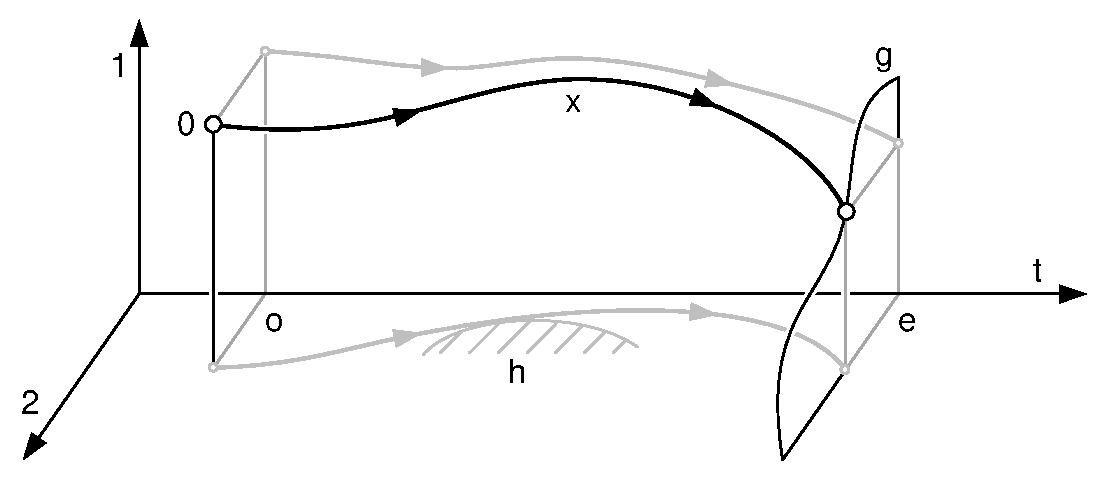
\includegraphics[width=1.\textwidth,clip, trim = 0cm 0cm 0cm 0cm]{2_Darstellung_dynamische_Optimierung_endvorgabe.eps}
  	\caption[Veranschaulichung der Lösung des Optimalsteuerungsproblems]{Veranschaulichung der Lösung $\bs{x}^\ast (t)\in \mathbb{R}^2$ eines Optimalsteuerungsproblems mit Endbedingung $\bs{g}=\bs 0$ und Ungleichungsbeschränkung $h\leq 0$ für $x_2$ sowie fester Endzeit $t_f$}
    \label{fig:dynamische_Optimierung_endvorgabe}
\end{figure}

Mit anderen Worten: Gesucht ist für ein (i.Allg.\ nichtlineares und zeitvariantes) System mit Zustand $\bs{x} \in \mathbb R^n$ und Eingang $\bs{u} \in \mathbb R^m$ auf dem Intervall $t\in[t_0, t_f]$ die Steuertrajektorie\index{Steuertrajektorie} $\bs{u}^\ast(t)$, die unter Minimierung des Kostenfunktionals\index{Kostenfunktional} $J$ das System vom Anfangszustand $\bs{x}_0$ in den Endzustand $\bs{x}(t_f)$ zur Endzeit $t_f$ steuert, sodass die Beschränkungen $\bs{h} \leq \bs{0}$ und Endbedingungen $\bs{g}= \bs{0}$ erfüllt sind, s.\ \abb{fig:dynamische_Optimierung_endvorgabe}. In der hier gewählten \emph{Bolza-Form} \cite{papageorgiou2012optimierung} setzt sich das Kostenfunktional \eqref{equ:opt_funktional} aus den Integralkosten $l$ und den Endkosten $V$ zusammen.\\
Die Endzeit $t_f$ ist entweder vorgegeben oder frei. Trifft letzteres zu, so ist $t_f$ Teil des Optimierungsproblems. Entfällt die Endbedingung $\bs{g}=\bs 0$, so wird von einem \emph{freien Endzustand} gesprochen. 
%Zur Veranschaulichung des Optimierungsproblems ist in \abb{fig:dynamische_Optimierung_endvorgabe} die optimale Trajektorie $\bs{x}^\ast(t)$ für eine feste Endzeit $t_f$ dargestellt. 
%In Bezug auf die f verschiedenen Auslegungsmöglichkeiten der Bestandteile des Optimalsteuerungsproblems im Hinblick auf das Trajektorien-Optimierungsproblem auf Fahrzeugführungsebene beleuchtet.

Zurückkehrend zu den Assistenzfunktionen der Führungsebene können die aufgeführten Bestandteile des Optimalsteuerungsproblems folgendermaßen ausgelegt werden:  Vereinfacht gesprochen\footnote{unter Vernachlässigung von Rückwirkungen der Bewegung des Eigenfahrzeugs auf die der anderen Verkehrsteilnehmer} findet sich die Fahrzeugdynamik und die daraus resultierende Bewegungskinematik im Systemmodell \eqref{equ:opt_systemdynamik} wieder. Unerwünschte Fahrzeugbewegungen, etwa das Abweichen von der Straßenmitte, gefährliche Fahrzustände, wie große Schwimmwinkel, und unkomfortable, hektische Lenkbewegungen sind im Kostenfunktional \eqref{equ:opt_funktional} zu bestrafen. Die Prädiktion der Fahrzeugumgebung wiederum fließt in die (aufgrund des dynamischen Fahrzeugumfelds \iA zeitvarianten) Ungleichungsbeschränkungen \eqref{equ:opt_ungleichungen} 
ein. Wie schon das Beispiel in Abb.\,\ref{fig:dynamische_Optimierung_endvorgabe} zeigt, kann darin die Kollisionsfreiheit inmitten von Hindernissen sichergestellt werden. Die Endbedingungen \eqref{equ:zm} können schließlich dazu genutzt werden, einen festen Zielzustand etwa auf einem Parkplatz vorzugeben. Darüber hinaus spielt die Wahl der Endkosten $V$ und der Ungleichungsbeschränkungen $\bs h$ eine entscheidende Rolle bei den Stabilitätsbetrachtungen in Abschn.\,\ref{sec:stab_mpc}.

\subsection{Modellprädiktiver Regelkreis\index{Modellprädiktiver Regelkreis}}
%[Unterbringen] Zur Erhöhung der Robustheit des Gesamtsystems gegen Störungen und Parameterschwankungen (Fahrbahnunebenheiten, nasse Fahrbahn), % und Ungenauigkeiten bei der Umsetzung der Trajektorie aufgrund von Parameterschwankungen und Modellvereinfachungen, 
%aber auch zur Berücksichtigung der jeweils aktuell verfügbaren Umfeldinformation empfiehlt sich eine permanente Neuplanung der Ausweichtrajektorie. Hierbei wird, im Unterschied zu einer initialen Einmalplanung, an der bis zum Manöverende festgehalten wird % (s.\ \zB 
%%\cite{keller2011active,% TITS Daimler, Polynome 7. Ordnung
%%isermann2008anticollision}, % sigmoiden
%%), 
%in jedem Zeitschritt der aktuelle Systemzustand in der Planung berücksichtigt, sodass aufgrund dieser Rückführung ein Regelkreis entsteht. \\
Erst durch eine permanente Berücksichtigung der aktuellen Umfeldinformationen ist eine optimale Navigation zwischen dynamischen Hindernissen möglich\footnote{Für singuläre Eingriffe wie dem Notausweichen existieren jedoch auch Forschungsansätze \cite{isermann2008anticollision, Bender2007, keller2011active}, die initial eine Trajektorie planen und an ihr bis zum Manöverende festhalten.}. Schließlich ist die Vorhersage der zukünftigen Bewegung anderer Verkehrsteilnehmer mit großen Unsicherheiten verbunden. Wie eingangs erwähnt, ermöglicht eine zyklische Optimierung aber auch die Reaktion auf unvorhergesehene Störungen bzw. Modellunsicherheiten. \\
Entsprechend der verbalen Beschreibung in Abschn.\,\ref{sec:def_modellpraediktive_Regelung} beruht die Funktionsweise eines modellprädiktiven Regelkreises genau darauf, dass in kurzen Abständen $\Delta t$ ein Optimalsteuerungsproblem über einen \iA mitgeführten Optimierungshorizont\index{Optimierungshorizont} der Länge $T$ gelöst wird \cite{gruene2011nonlinear, Johansen2011, Findeisen2002, graichen2014SkriptOpt}. 
Der entsprechend des Systemzustands $\bs x(t_k)$ optimierte Stellgrößenverlauf $\bar{\bs u}(\tau)^\ast, \tau \in [t_k, t_k+T]$ wird dabei in jedem Schritt nur für das Intervall $t\in [t_k, t_k+\Delta t)$ gestellt, da danach bereits das Ergebnis des nächsten Optimierungsschritts vorliegt, s.\ Abb.\,\ref{fig:2_mpc_grundidee_u_x}.
\begin{figure}[h]
\centering
    \psfrag{x}[lb][lb][1.]{$\bs x(t)$}
		\psfrag{s}[lb][lb][1.]{$\bar{\bs x}^\ast(\tau)$}
		\psfrag{u}[lt][lt][1.]{$\bs u(t)$}
		\psfrag{w}[lt][lt][1.]{$\bar{\bs u}^\ast(\tau)$}
		\psfrag{V}[tr][tr][1.]{Vergangenheit}
		\psfrag{Z}[tl][tl][1.]{Zukunft}
		\psfrag{D}[tc][tc][1.]{$\Delta t$}
		\psfrag{T}[tc][tc][1.]{Optimierungshorizont $T$}
		\psfrag{t}[tc][tc][1.]{$t,\tau$}
		\psfrag{k}[tc][tc][1.]{$t_k$}
		\psfrag{1}[tc][tc][1.]{$t_{k-1}$}
		\psfrag{2}[tc][tc][1.]{$t_{k-2}$}
		\psfrag{3}[tc][tc][1.]{$t_{k-3}$}
	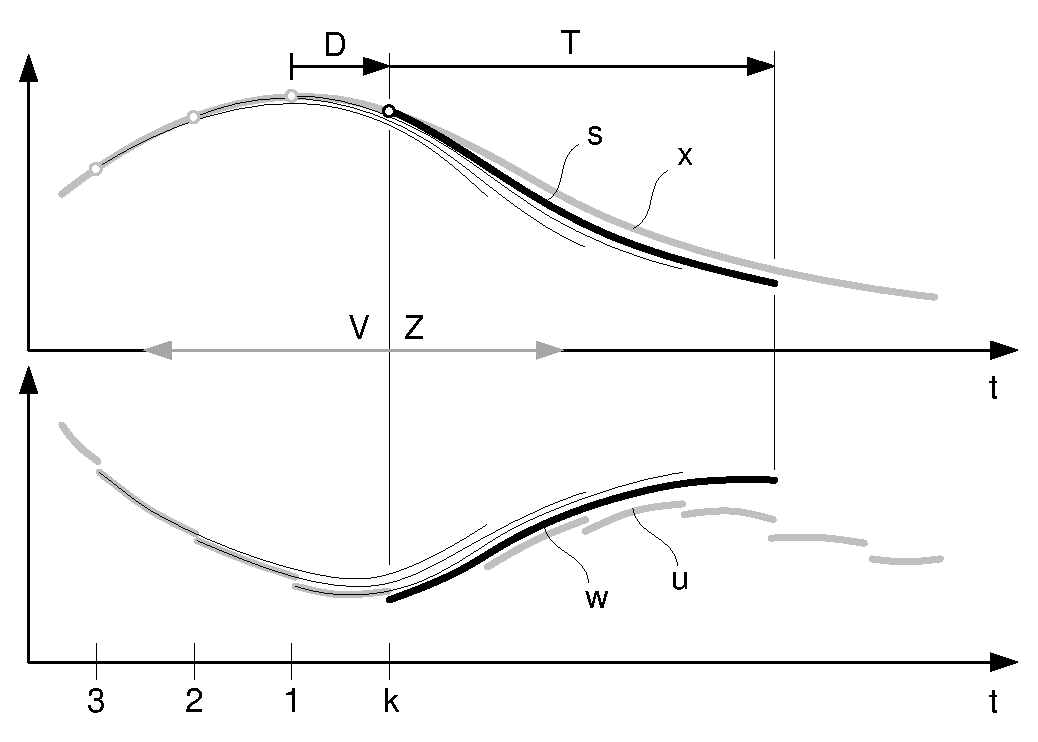
\includegraphics[width=1.\textwidth,clip, trim = 0cm 0cm 0cm 0cm]{2_mpc_grundidee_u_x.eps}
	\caption[Grundidee der modellprädiktiven Regelung]{Grundidee der modellprädiktiven Regelung; dick, schwarz: intern zum Zeitpunkt $t_k$ optimierte Zustands- und Stellgrößenverläufe; dünn, schwarz:  intern optimierte Verläufe der Vergangenheit; dick, grau: sich tatsächlich ergebende Verläufe des geschlossenen Regelkreises, vgl.\ \cite{graichen2014SkriptOpt}}
	\label{fig:2_mpc_grundidee_u_x}
\end{figure}

Mit dem Optimierungshorizont\index{Optimierungshorizont} $T$ und den darauf prädizierten Modellgrößen $\bar{\bs{x}}, \bar{\bs{u}}$ stellt sich das schritthaltend zu lösende Optimalsteuerungsproblem als
\begin{subequations} \label{equ:mpc_problem}
\begin{align}
	\underset{\bar{\bs{u}}(\cdot)}{\text{minimiere}}  \quad & %J(\bs{\phi}(t,\bar{\bs{u}}),\bs{\psi}(t,\bar{\bs{u}}),t)) = 
	\int_{t_k}^{t_k+T} l(\bar{\bs x}(\tau), \bar{\bs u}(\tau),\tau)\,{\rm d} \tau\,\,+\,\, V(\bar{\bs{x}}(t_k+T),t_k+T) \label{equ:mpc_funktional}\\
	\text{u.B.v.} \quad &\dot{\bar{\bs{x}}}(\tau) = \bs{f}(\bar{\bs{x}}(\tau),\bar{\bs{u}}(\tau),\tau), \quad \bar{\bs{x}}(t_k) = \bs{x}(t_k) \label{equ:mpc_system}\\\
\quad &\bs{g}(\bar{\bs{x}}(t_k+T),t_k+T) = \bs{0} \label{equ:mpc_gnb}\\ 	
	&\bs{h}(\bar{\bs{x}}(\tau),\bar{\bs{u}}(\tau),\tau) \leq \bs{0},  \quad \forall \tau \in[t_k, t_k + T] \label{equ:mpc_unb}
\end{align} 
\end{subequations}
dar. Aus Sicht der Optimierung gibt es keine algorithmischen Unterschiede zu \eqref{equ:optimalsteuerungsproblem}, weshalb sich die Kap.\,\ref{chap:dynamische_Optimierung_dynamisch}, \ref{chap:dynamische_Optimierung_direkt} und \ref{chap:dynamische_Optimierung_indirekt} auf das übersichtlichere Optimalsteuerungsproblem \eqref{equ:optimalsteuerungsproblem} beziehen. 

%\subsection{Systembeschreibung} \label{sec:direkte_methode_systembeschreibung}
%Nachstehend werden die verschiedenen Auslegungsmöglichkeiten der Bestandteile des Optimalsteuerungsproblems im Hinblick auf das Trajektorien-Optimierungsproblem auf Fahrzeugführungsebene beleuchtet und anhand von Literaturbeispielen aus dem Bereich des hochautomatisierten Fahrens und der Fahrerassistenz belegt. Wenn immer nötig werden hierbei, als Vorgriff auf die anschließenden Kapitel, Hinweise darauf gegeben, welchen Einfluss das angewendete Optimierungsverfahren hat. \\

% Inhalt:
% - Wahl der Zustandsgrößen abhängig von Optimierungsansatz
% - So wenige wie möglich, dass gerade noch so der Kern des Optimierungsproblems getroffenwird -> Hierarchische verbesserung
%


%Slackvariablen mit schönem Bild aus MPC
%\subsection{Einteilung der Lösungsmethodik} % ggf. nur überführende Bemerkung zu nächsten Kapitel, mit Anmerkung, dass zunächst noch Stabi. und Robustheit betrachtet wird.
% DP, dirO, indirO:
% DB: zeit- und wertdiskretes u (Anwendung)s
% dirO: zeitdiskretes u
% indir: kontinuierliche Verläufe

\section{Realisierbarkeits- und Stabilitätsbetrachtungen} \label{sec:stab_mpc}
Basiert der Regelkreis auf der Lösung eines Optimalsteuerungsproblems mit \emph{unendlich} langem Optimierungshorizont, dann weist er ganz besondere Eigenschaften auf. Insbesondere stimmen, in Abwesenheit von Störungen und Modellfehlern, in jedem Schritt die prädizierten Systemverläufe mit den tatsächlichen überein, was sich leicht mit dem später in Abschn.\,\ref{sec:bellman} vorgestellten \emph{Bellman'schen Optimalitätsprinzip} erklären lässt. Hiermit sichert die Lösbarkeit des Optimierungsproblems im Anfangszustand die Lösbarkeit für alle folgenden
Zeitschritte.
Dieser Sachverhalt wird in der Literatur auch als \emph{rekursive}\index{rekursive Lösbarkeit} oder \emph{anhaltende Lösbarkeit} (\emph{recursive}, \emph{persistent feasibility}) bezeichnet \cite{borrelli2014predictive, gruene2011nonlinear}. Des Weiteren garantiert ein unendlicher Optimierungshorizont unter recht allgemeinen Bedingungen \cite{borrelli2014predictive, gruene2011nonlinear, Findeisen2002} einen \emph{stabilen} Regelkreis, s.\ Abschn.\,\ref{sec:stabilität}. \\
Im Unterschied dazu beschränkt sich der modellprädiktive Regelkreis (aus Rechenzeitgründen) auf einen \emph{endlichen} Optimierungshorizont, der  
\iA zu einer \emph{Diskrepanz} zwischen den Lösungen der aufeinanderfolgenden Optimierungsschritte führt, s.\ Abb.\,\ref{fig:2_mpc_grundidee_u_x}. Die Hoffnung ist, dass sich die Einbußen der beschränkten Vorausschau in Bezug auf das Gütekriterium, aber auch auf die rekursive Lösbarkeit und die Stabilität in Grenzen halten. Wie nachfolgend anhand eines modellprädiktiven Abstandsregeltempomats (ACC) verdeutlicht wird, bewahrt die bloße Optimierung jedoch keinesfalls davor, dass sich der modellprädiktive Regelkreis in Situationen bringt, die nicht mehr lösbar sind, obwohl (anfänglich) eine Lösung für das Optimierungsproblem mit unendlichem Horizont existiert hat.
Wie ebenfalls simulativ verdeutlicht wird, ist die Stabilität des modellprädiktiven Regelkreises (selbst bei gegebener Lösbarkeit) nicht gesichert, sodass sich das geregelte System aufschwingen kann.
%Nachfolgend wird aufgrund der hochgradigen Relevanz der modellprädiktiven Regelung in der Fahrerassistenz für die beschriebene Problematik weiter sensibilisiert. 
Es existieren jedoch auf der Lyapunov-Stabilitätstheorie\index{Lyapunov-Stabilität} basierende MPC-Schemata \cite{borrelli2014predictive, gruene2011nonlinear, Findeisen2002}, die durch geeignete Modifikation der Optimierungskosten und Nebenbedingungen die rekursive Lösbarkeit und Stabilität garantieren. Ein recht allgemeiner und gleichzeitig gut auf Fahrerassistenzprobleme übertragbarer Ansatz wird vorgestellt und auf das ACC-Regelungsproblem gewinnbringend angewandt. 

\subsection{Beispiel modellprädiktiver Abstandsregeltempomat} \label{sec:mpc_acc}
Das Ziel eines Abstandsregeltempomaten\index{Abstandsregeltempomat} (\emph{Adaptive Cruise Control}, ACC) ist, eine vom Fahrer eingestellte Sollgeschwindigkeit einzuregeln (Tempomatfunktion), ohne dass ein vorgegebener Sollabstand zum vorausfahrenden Fahrzeug dauerhaft unterschritten wird. Eine Regelung mit unterschiedlichen Regelzielen wird auch als \emph{override control}\index{override control} bezeichnet \cite{glattfelder1983soc} und lässt sich im vorliegenden Fall dadurch realisieren, dass sich mittels
\begin{align*}
	u(\bs x) = \min(r_v(\bs x), r_d(\bs x))
\end{align*}
immer das stärker bremsende bzw.\ weniger starke beschleunigende Regelgesetz auf die Aktorik durchschlägt \cite{atSonderheft08, handbuchFAS_Winner}. Da für die Lösbarkeits- und Stabilitätsbetrachtungen das Abstandsregelgesetz $r_d(\bs x)$ von größerem Interesse ist als das Geschwindigkeitsregelgesetz $r_v(\bs x)$, wird auf ersteres eingegangen. Die Rückführung $r_d(\bs x)$ soll hier als modellprädiktiver Regler ausgeführt werden, dessen Optimierungskriterium \eqref{equ:mpc_funktional} sowie Fahrzeugmodell \eqref{equ:mpc_system} und die daran gestellten Ungleichungsnebenbedingungen \eqref{equ:mpc_unb} nachfolgend hergeleitet werden. Für die eigentliche Lösung der Optimierungsaufgabe muss jedoch auf die nachfolgenden Kapitel verwiesen werden.

\begin{figure}[h]
\centering
    \psfrag{A}[tc][tc][1.]{Ist-Position}
		%\psfrag{B}[tc][tc][1.]{\parbox[t]{3cm}{Soll-Position \\ ($\Delta x = 0$)}}
		\psfrag{B}[tc][tc][1.]{Soll-Position}
		\psfrag{C}[tc][tc][1.]{Vorderfahrzeug}
		\psfrag{D}[cc][cc][1.]{$\Delta x = 0$}
    \psfrag{1}[bc][bc][1.]{$v_v$}
		\psfrag{2}[bc][bc][1.]{$v_\text{ego}$}
		\psfrag{3}[bc][bc][1.]{$x_v$}
		\psfrag{4}[bc][bc][1.]{$x_\text{ego}$}
		\psfrag{5}[bc][bc][1.]{$d$}
	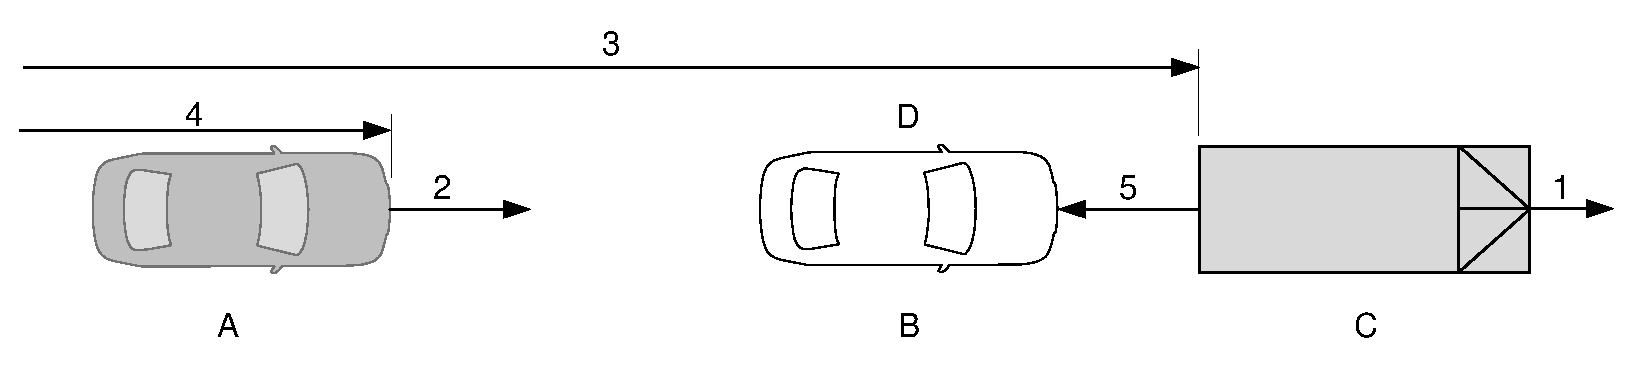
\includegraphics[width=1.\textwidth,clip, trim = 0cm 0cm 0cm 0cm]{3_ACC_topview.eps}
	\caption{Systemgrößendefinition der modellprädiktiven Abstandsregelung}
	\label{fig:ACC_topview}
\end{figure}

Es sei Abb.\,\ref{fig:ACC_topview} betrachtet, in der die Längsposition der Ego-Fahrzeugfront  $x_\text{ego}$ und des Vorderfahrzeughecks $x_v$ eingezeichnet sind. Da für die Funktion nur Relativgrößen von Belang sind, wird für das Systemmodell der Systemzustand $\Delta x =  x_\text{ego} - [x_v-d]$ eingeführt, der die Regelabweichung von der durch den Sollabstand $d$ definierten Sollposition $[x_v-d]$ beschreibt. Ist das Regelziel erreicht, dann befindet sich das Egofahrzeug, wie in Abb.\,\ref{fig:ACC_topview} in Weiß dargestellt, bei $\Delta x=0$.
Die zeitliche Änderung von $\Delta x$ wird wiederum von der relativen Annäherungsgeschwindigkeit $\Delta v = v_\text{ego} - v_v$ beschrieben. Vereinfachend gilt für die Vorderfahrzeuggeschwindigkeit $v_v = \text{const.}$ , d.h.\ der vorausfahrende Verkehr beschleunigt oder verzögert nicht\footnote{Abweichungen von diesem Verhalten stellen Störungen dar, die durch Modifikation des im Folgenden beschriebenen Herangehens behandelt werden können, vgl.\ \cite{dold2010robuste}.}.  Aus Komfortgründen muss die Ego-Längsbeschleunigung später im geschlossenen Regelkreis stetig verlaufen, was dadurch sichergestellt werden kann, dass sie als Systemzustand $a_\text{ego}$ aufgefasst wird, s.\ später hierzu auch Abb.\,\ref{fig:KR_Integrator_Erweiterung}. Insgesamt lässt sich damit die Annäherungsdynamik mit dem linearen, zeitinvarianten System 
%$\bs x = [\Delta x, \Delta v, a]$, $u$ Ruck
\begin{align}\label{equ:acc_sys}
	\dot{\bs x} = %\bs f(\bs x, u) = 
	\bs A \bs x + \bs b u \quad \text{mit} \quad \bs x = \mtrx{c}{\Delta x \\ \Delta v \\ a_\text{ego}} \!\! , \; \bs A = \mtrx{ccc}{0 & 1 & 0 \\ 0 & 0 & 1 \\ 0 & 0 & 0 } \text{und} \;\; \bs b = \mtrx{c}{ 0 \\ 0 \\ 1 }
\end{align}
beschreiben, wobei der Längsruck $j_\text{ego}=\dot a_\text{ego}(t)$ den Systemeingang $u$ darstellt. \\
Die von der Aufgabenstellung herrührenden zeitinvarianten Ungleichungsnebenbedingungen setzen sich aus der Kollisionsfreiheit mit dem Vorderfahrzeug $(\Delta x(t) \leq d)$ und dem beschränkten Beschleunigungs- und Verzögerungsvermögen $(a_{\min} \leq a(t) \leq a_{\max})$ zusammen, die sich %$\bs x = [x_1, x_2, x_3]^\T$
 kompakt als
%\begin{align*}
	%\bs g(\bs x) = \mtrx{c}{x_1 \\ x_3 \\ -x_3} \leq \mtrx{c}{d \\ a_{\max}  \\ -a_{\min}}
%\end{align*}
%
\begin{align} \label{equ:acc_unb}
	%\bs g(\bs x) = 
	\bs A_c \bs x - \bs b_c \leq \bs 0 \quad \text{mit} \quad \bs A_c = \mtrx{ccc}{1 & 0 & 0 \\ 0 & 0 & 1 \\ 0 & 0 & -1 } \text{und} \;\; \bs b_c = \mtrx{c}{ d \\ a_{\max}  \\ -a_{\min} }
\end{align}
darstellen lassen.

Schließlich werden die im Kostenfunktional \eqref{equ:mpc_funktional} des modellprädiktiven Reglers auftretenden Integralkosten in quadratischer Form zu
\begin{align}
	l(\bs{x},u) &= \bs x^\T \bs Q_\text{acc} \bs x + R_\text{acc} u^2 \quad \text{mit} \quad \bs Q_\text{acc} =  \bs Q_\text{acc}^\T > 0 \; \text{und} \; R_\text{acc} > 0 \label{equ:acc_integral}
	%V(\bs x(t_f)) &= \bs x(t_f)^\T \bs P \bs x(t_f) \quad \text{mit} \quad \bs P\succ 0 \;,
\end{align}
gewählt, sodass Abweichungen von der Sollposition $\Delta x = 0$ und deren zeitliche Ableitungen bestraft werden. Bei $\bs Q_\text{acc}$ handelt es sich somit um eine symmetrische, positiv definite\footnote{Eine Matrix $\bs A$ ist positiv definit, falls $\bs x^\T \bs A \bs x > \bs 0 \; \forall \bs x \in \mathbb R^n \setminus \{\bs 0\}$ und $\bs x^\T \bs A \bs x = \bs 0$ für $\bs x = \bs 0$; gilt anstelle des Vergleichsoperators $>$ nur $\geq$, so ist $\bs A$ positiv semidefinit. }  Matrix. Auf einen Endkostenterm $V(\bs x(t_f))$ in \eqref{equ:mpc_funktional} wird in einem ersten Ansatz zunächst verzichtet. \\
Mit \eqref{equ:acc_sys}, \eqref{equ:acc_unb} und \eqref{equ:acc_integral} ergibt sich für \eqref{equ:mpc_problem} ein sog.\ linear-quadratisches Optimierungsproblem (lineares Systemmodell, quadratisches Kostenfunktional) mit linearen Nebenbedingungen, das mit den später in Abschn.\,\ref{sec:direkte_einfach_schiessverfahren} beschriebenen Verfahren effizient gelöst werden kann. 
Damit wird der modellprädiktive Regelkreis geschlossen und aus der Streckendynamik $\dot{\bs x} = \bs f(\bs x, u)$ entsteht ein autonomes System $\dot{\bs x} = \bs f(\bs x, r_d(\bs x))$. Von der Umfeldsensorik neu erkannte Vorderfahrzeuge führen folglich zu Anfangsfehlern $\bs{x}_0$, die das System zu $\bs x_s = \bs 0$ abbauen muss, um den Sollabstand einzuregeln.

Die Optimierung erfolgt mit einer Zykluszeit von $\unit[100]{ms}$ und der Optimierungshorizont wird zunächst auf $T = \infty$ gesetzt\footnote{In guter Näherung wird in der numerischen Optimierung der Horizont auf $\unit[100.0]{s}$ begrenzt, da darüber hinaus keine nennenswerten Veränderungen in den Ergebnissen beobachtet werden können.}. In Abb.\,\ref{fig:3_MPC_Infeasable} ist das entsprechende Simulationsergebnis für einen um $\unitfrac[20]{m}{s}$ langsameren Einscherer\footnote{in die Ego-Spur wechselndes Vorderfahrzeug} dargestellt, der $\unit[25]{m}$ vor dem Ego-Fahrzeug erkannt wird, sodass die Situation ein drastisches Bremsen erfordert. Wie der hellgrauen 2d-Projektion entnommen werden kann, überführt der unendliche Optimierungshorizont das Fahrzeug von $\bs x_0 = [\unit[-15.0]{m}, \unitfrac[20.0]{m}{s}, \unitfrac[0.0]{m}{s^2}]$ in den Ursprung (Stern), sodass sich der Sollabstand von $d=\unit[10.0]{m}$ einstellt. Dabei werden zwei der Ungleichungsnebenbedingungen aktiv, wie später den hellgrauen Signalverläufen in Abb.\,\ref{fig:MPC_Signals} auf S.\,\pageref{fig:MPC_Signals} entnommen werden kann. Sie können aber zu jedem Zeitpunkt eingehalten werden, sodass weder die zulässige Verzögerung überschritten, noch das Vorderfahrzeug berührt werden. Aufgrund des Bellman'schen Optimalitätsprinzips folgt hierbei das System in jedem Schritt der zuvor optimierten Trajektorie, sodass in der Abbildung keine Diskrepanz zwischen geplanter und tatsächlicher Trajektorie erkennbar ist.

\begin{figure}[ht]
	%\centering
	% Erste Figure	
	\def\xlabel{$\Delta x$ in $\unit{m}$}
	\def\vlabel{$\Delta v$ in $\unitfrac{m}{s}$}	
	\def\alabel{$\mathcal{C}_\infty$}
	\def\blabel{ICS}
	\def\x0{$\bs x_0$}
	% Generated using matlabfrag
% Version: v0.6.16
% Version Date: 04-Apr-2010
% Author: Zebb Prime
%
%% <text>
%
\providecommand\matlabtextA{\color[rgb]{0.000,0.000,0.000}\fontsize{10}{10}\selectfont\strut}%
\psfrag{009}[cl][cl]{\matlabtextA \x0}%
\psfrag{010}[cl][cl]{\matlabtextA \blabel}%
\psfrag{011}[cl][cl]{\matlabtextA \alabel}%
\psfrag{012}[bc][bc]{\matlabtextA \vlabel}%
\psfrag{013}[tc][tc]{\matlabtextA \xlabel}%
%
%% </text>
%
%% <xtick>
%
\def\matlabfragNegXTick{\mathord{\makebox[0pt][r]{$-$}}}
%
\psfrag{000}[ct][ct]{\matlabtextA $\matlabfragNegXTick 20$}%
\psfrag{001}[ct][ct]{\matlabtextA $\matlabfragNegXTick 10$}%
\psfrag{002}[ct][ct]{\matlabtextA $0$}%
\psfrag{003}[ct][ct]{\matlabtextA $10$}%
%
%% </xtick>
%
%% <ytick>
%
\psfrag{004}[rc][rc]{\matlabtextA $-10$}%
\psfrag{005}[rc][rc]{\matlabtextA $0$}%
\psfrag{006}[rc][rc]{\matlabtextA $10$}%
\psfrag{007}[rc][rc]{\matlabtextA $20$}%
\psfrag{008}[rc][rc]{\matlabtextA $30$}%
%
%% </ytick>
	%\renewcommand{\matlabtextA}{\scriptsize}
	%\renewcommand{\matlabtextB}{\scriptsize}
    \subfigure[Rekursive Unlösbarkeit für $T=0.5 {\rm s}$]{
		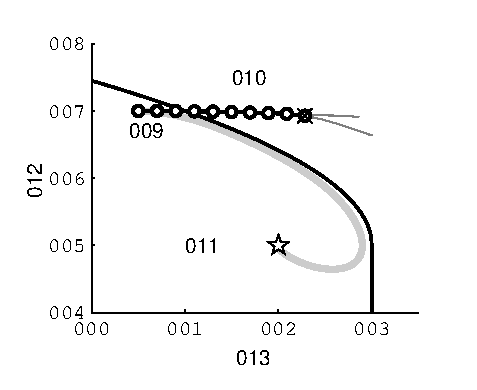
\includegraphics[width=.5 \linewidth,trim = 0cm 0cm 0cm 0cm]{3_MPC_Infeasable.eps}\label{fig:3_MPC_Infeasable}} %\\[3ex]
	% Zweite Figure	
	\def\dots{$(\ldots)$}
	% Generated using matlabfrag
% Version: v0.6.16
% Version Date: 04-Apr-2010
% Author: Zebb Prime
%
%% <text>
%
\providecommand\matlabtextA{\color[rgb]{0.000,0.000,0.000}\fontsize{10}{10}\selectfont\strut}%
\psfrag{009}[cl][cl]{\matlabtextA \dots}%
\psfrag{010}[cl][cl]{\matlabtextA \x0}%
\psfrag{011}[bc][bc]{\matlabtextA \vlabel}%
\psfrag{012}[tc][tc]{\matlabtextA \xlabel}%
%
%% </text>
%
%% <xtick>
%
\def\matlabfragNegXTick{\mathord{\makebox[0pt][r]{$-$}}}
%
\psfrag{000}[ct][ct]{\matlabtextA $\matlabfragNegXTick 2$}%
\psfrag{001}[ct][ct]{\matlabtextA $\matlabfragNegXTick 1$}%
\psfrag{002}[ct][ct]{\matlabtextA $0$}%
\psfrag{003}[ct][ct]{\matlabtextA $1$}%
\psfrag{004}[ct][ct]{\matlabtextA $2$}%
%
%% </xtick>
%
%% <ytick>
%
\psfrag{005}[rc][rc]{\matlabtextA $-0.4$}%
\psfrag{006}[rc][rc]{\matlabtextA $-0.2$}%
\psfrag{007}[rc][rc]{\matlabtextA $0$}%
\psfrag{008}[rc][rc]{\matlabtextA $0.2$}%
%
%% </ytick>
    \subfigure[Instabilität für $T=0.5 {\rm s}$]{
		
\includegraphics[width=.5 \linewidth,trim = 0cm 0cm 0cm 0cm]{3_MPC_Instable.eps}
		\label{fig:3_MPC_Instable}}
	% Beschriftung
    \caption[Trajektorien des modellprädiktiven ACC-Regelkreises]{2d-Projektion der Trajektorien des modellprädiktiven Regelkreises; $T = \infty$ in Grau, $T=\unit[0.5]{s}$ mit weißen Punkten; Modellprädiktionen in dünnen, grauen Linien; $d = \unit[10.0]{m}$,
$a_{\min} = -\unitfrac[10.0]{m}{s^2}$,
$a_{\max} = \unitfrac[5.0]{m}{s^2}$,
$\bs Q_\text{acc} = \text{diag}(1,1,1)$,
$R_\text{acc} = 1$ (links), $R_\text{acc} = 5$ (rechts)}
\end{figure}

Ganz anders verhält sich ein auf $T = \unit[0.5]{s}$ reduzierter Optimierungshorizont. Aufgrund der kurzsichtigen Arbeitsweise nimmt die Optimierung erst nach $\unit[0.9]{s}$ Simulationszeit (neunter weißer Punkt in Abb.\,\ref{fig:3_MPC_Infeasable}) Notiz von der brenzligen Lage, sodass schon im zehnten Schritt keine Lösung des Optimalsteuerungsproblems mehr existiert (weißer Punkt mit Kreuz). Das verwundert nicht weiter, da sich das System  im vierten Schritt längst oberhalb der schwarzen Linie befindet, welche den Übergang zu der bereits in Abb.\,\ref{fig:ausweichen_vs_bremsen} auf S.\,\pageref{fig:ausweichen_vs_bremsen} abgebildeten ICS-Menge darstellt, den Zuständen einer unvermeidlichen Kollision. Die rekursive Lösbarkeit ist somit nicht gegeben und das Fahrzeug wird in der Realität kollidieren. \\
Ebenso wenig kann, selbst bei inaktiven Nebenbedingungen, die Stabilität des Regelkreises mit $T = \unit[0.5]{s}$ garantiert werden, wie dessen 2d-projizierte Systemtrajektorie in Abb.\,\ref{fig:3_MPC_Instable} verdeutlicht. Im Unterschied zur Regelung mit $T = \infty$ (hellgrau), die das System aus $\bs x_0 = [\unit[1.0]{m}, 0, 0]$ stabil in den Ursprung bringt, führt der kurze Optimierungshorizont zu einem Aufschwingen des Systems (weiße Punkte).

Zwar gibt es für bestimmte Problemklassen immer eine Grenze für $T$, oberhalb derer rekursive Lösbarkeit und Stabilität sichergestellt ist. Ihre Bestimmung ist jedoch mathematisch aufwändig \cite{graichen2014SkriptOpt} und überhaupt verbietet die verfügbare Rechenleistung häufig einen derart langen Optimierungshorizont. 
Um trotz eines kurzen Optimierungshorizonts ein gutes Ergebnis zu erzielen, existieren in der modernen Regelungstheorie Techniken, die Endkosten $V(\bs x(t_k\!+\!T), t_k\!+\!T)$ und Zielmengen für $\bs x(t_k\!+\!T) \in \mathcal{X}_f$ so vorgeben, dass der modellprädiktive Regler über den Optimierungshorizont hinaus auf das "`Kommende"' vorbereitet wird und Stabilität und rekursive Lösbarkeit gesichert sind. Wie sich bereits im ACC-Beispiel angekündigt hat, existieren hierbei Parallelen zu Methoden der Robotik, auch wenn dort die Stabilität typischerweise nicht im Fokus steht.

Nacheinander werden nun die wichtigsten Grundlagen geschaffen und in einem MPC-Schema kombiniert, das das Verhalten einer modellprädiktiven Regelung mit beschränktem Optimierungshorizont drastisch verbessert. Die Grundlagen und das Schema werden anhand des Abstandsregeltempomaten veranschaulicht.
%Das angewandte Konzept wird schließlich verallgemeinert, wobei Hinweise darauf gegeben werden, worin die Herausforderungen bei dessen praktischer Umsetzung bei zeitvarianten Systemen bestehen.

\subsection{Invariante Mengen\index{Invariante Menge}} \label{sec:invariantSets}
Der folgende Abschnitt bezieht sich wieder auf das Optimalsteuerungsproblem \eqref{equ:optimalsteuerungsproblem}. 
In vielen praktischen Aufgabenstellungen kann darin die sehr allgemeine Form \eqref{equ:opt_ungleichungen} der Ungleichungsbeschränkungen so abgewandelt werden, dass der Eingang $\bs u(t)$ und der Zustand $\bs x(t)$ nur noch unabhängig voneinander beschränkt sind und sich
\begin{alignat*}{2}
	{\bs x}(t) &\in \mathcal X \subseteq \mathbb R^n, & \quad {\bs u}(t) \in \mathcal U \subseteq \mathbb R^m; \quad \forall t &\in [t_0, t_f] %\\
	%\bar{\bs x}(\tau_f) &\in \mathcal X_f; & \quad \tau_f &= t_k + T
\end{alignat*}
schreiben lässt. %wobei $\mathcal X \subseteq \mathbb R^n$ und $\mathcal U\subseteq\mathbb R^m$ die Zustands- und Stellgrößenbeschränkungsmengen und $\mathcal X_f\subseteq \mathbb R^n$ die häufig als Endregion bezeichnete Zielmenge darstellen. 
In unmittelbarem Zusammenhang steht damit folgende Definition \cite{borrelli2014predictive}:

\begin{mydef}
Die Menge $\mathcal C \subseteq \mathcal X$ eines Systems \eqref{equ:opt_systemdynamik} mit Zustands- und Stellgrößenbeschränkungsmenge $\mathcal X, \mathcal U$ wird  als \emph{control-invariant} bezeichnet, wenn
\begin{align*}
	\bs x(0) \in \mathcal C \,\,  \Rightarrow \,\,  \exists \bs u(t) \in \mathcal U, \,\text{sodass} \, \bs x(t) \in \mathcal C \, ,\forall t \geq 0 
\end{align*}
gilt.
\end{mydef}
Für jedes Element der invarianten Zustandsmenge $\mathcal C$ gibt es also ein Stellgrößensignal $\bs u(t)$, sodass die Trajektorie $\bs x(t)$ die Zustandsmenge $\mathcal C$ nie verlässt.

% Falcone Threat ass. (11)
Wird der Systemzustand von \eqref{equ:opt_systemdynamik} mit einem Regler $\bs u = \bs r(\bs x)$ auf die Stellgröße rückgeführt, so entsteht wie im vorherigen Abschnitt ein \emph{autonomes} System. Existieren für die Regelstrecke Stellgrößenbeschränkungen, so werden sie im autonomen System Teil der Zustandsgrößenbeschränkung $\mathcal X$.
Ein autonomes System besitzt definitionsgemäß keinen Eingang, womit sich die Invarianz-Definition \cite{borrelli2014predictive} entsprechend vereinfacht:

\begin{mydef}
Für ein autonomes System $\dot {\bs x} = \bs f(\bs x)$ mit Zustandsbeschränkungsmenge $\mathcal X$ wird eine Menge  $\mathcal O \subseteq \mathcal X$ als \emph{positiv invariant} bezeichnet, wenn
\begin{align*}
	\bs x(0) \in \mathcal O \,\,  \Rightarrow \,\,  \bs x(t) \in \mathcal O, \, \forall t \geq 0 
\end{align*}
gilt. 
\end{mydef}
Demnach bleibt jede Trajektorie mit Anfangszustand in der invarianten Menge $\mathcal O$ für alle Zeit darin.

\begin{mydef}
Die \emph{Vereinigung} aller invarianten Mengen eines Systems wird als \emph{maximale invariante Menge} $\mathcal C_{\infty}$ \bzw  $\mathcal O_{\infty}$ bezeichnet \cite{borrelli2014predictive}. %
\end{mydef}

Aufgrund der linearen, zeitinvarianten Fahrzeuglängsdynamik \eqref{equ:acc_unb} gepaart mit den linearen Ungleichungsnebenbedingungen \eqref{equ:acc_unb} für $\mathcal X \subset \mathbb R^3$ lässt sich durch zeitliche Diskretisierung die maximale invariante Menge $\mathcal C_{\infty} \subset \mathcal X$ des ACC-Problems effizient mittels \cite{herceg2013multi} berechnen. Das Ergebnis ist in Abb.\,\ref{fig:C_inf_und_O_inf_LQR} als durchsichtiges Drahtgittermodell dargestellt, das bei $\Delta x = -\unit[150]{m}$ und $\Delta v = -\unitfrac[15]{m}{s}$ gestutzt wurde, da es sich aufgrund der Abwesenheit von Nebenbedingungen in diese Richtungen bis ins Unendliche fortsetzt. 
Eine bei $a_\text{ego} = 0\, \unitfrac{m}{s^2}$ entnommene Scheibe ist daneben in Abb.\,\ref{fig:MPC_Konvergenz} abgebildet. Auch hier sei darauf hingewiesen, dass aus Darstellungsgründen die Mengen zusätzlich zu den vorherigen Grenzen auch oberhalb von $\unitfrac[60]{m}{s}$ abgeschnitten sind. Aus der Abbildung
wird sofort der Zusammenhang
\begin{align}
	\mathcal C_\infty = \mathcal X \setminus \text{ICS}
\end{align}
ersichtlich. Die maximale invariante Menge $\mathcal C_\infty$ beinhaltet nämlich alle Zustände, die durch ein Stellgesetz überhaupt vor einer Verletzung der Nebenbedingung bewahrt werden können. Außerhalb führen alle Zustände %$\bs x\in \mathcal X$ 
zu einer Verletzung der Nebenbedingung, wie auch immer $u(t)$ gewählt wird, und liegen damit in der ICS-Menge, kollidieren also im Beispiel unweigerlich mit dem Vorderfahrzeug. 

\begin{figure}[ht]
	%\centering
	% Erste Figure	
	\def\xlabel{$\Delta x$ in $\unit{m}$}
	\def\vlabel{$\Delta v$ in $\unitfrac{m}{s}$}	
	\def\alabel{$a_\text{ego}$ in $\unitfrac{m}{s^2}$}	
	% Generated using matlabfrag
% Version: v0.6.16
% Version Date: 04-Apr-2010
% Author: Zebb Prime
%
%% <text>
%
\providecommand\matlabtextA{\color[rgb]{0.000,0.000,0.000}\fontsize{10}{10}\selectfont\strut}%
\psfrag{012}[bc][bc]{\matlabtextA \alabel}%
\psfrag{013}[tr][tr]{\matlabtextA \vlabel}%
\psfrag{014}[tl][tl]{\matlabtextA \xlabel}%
%
%% </text>
%
%% <xtick>
%
\def\matlabfragNegXTick{\mathord{\makebox[0pt][r]{$-$}}}
%
\psfrag{000}[ct][ct]{\matlabtextA $\matlabfragNegXTick 150$}%
\psfrag{001}[ct][ct]{\matlabtextA $\matlabfragNegXTick 100$}%
\psfrag{002}[ct][ct]{\matlabtextA $\matlabfragNegXTick 50$}%
\psfrag{003}[ct][ct]{\matlabtextA $0$}%
%
%% </xtick>
%
%% <ytick>
%
\psfrag{004}[rc][rc]{\matlabtextA $0$}%
\psfrag{005}[rc][rc]{\matlabtextA $20$}%
\psfrag{006}[rc][rc]{\matlabtextA $40$}%
\psfrag{007}[rc][rc]{\matlabtextA $60$}%
%
%% </ytick>
%
%% <ztick>
%
\psfrag{008}[cr][cr]{\matlabtextA $-10$}%
\psfrag{009}[cr][cr]{\matlabtextA $-5$}%
\psfrag{010}[cr][cr]{\matlabtextA $0$}%
\psfrag{011}[cr][cr]{\matlabtextA $5$}%
%
%% </ztick>
	%\renewcommand{\matlabtextA}{\scriptsize}
	%\renewcommand{\matlabtextB}{\scriptsize}
    \subfigure[Invariante Mengen]{
		\includegraphics[width=.55 \linewidth,trim = 0cm 0cm 0cm 0cm]{3_C_inf_und_O_inf_LQR.eps}\label{fig:C_inf_und_O_inf_LQR}} %\\[3ex]
		\!\!\!\!\!\!\!\!\!\!\!\!
	% Zweite Figure	
	%\def\xlabel{$x$ in $\unit{m}$}
	%\def\vlabel{$v$ in $\unitfrac{m}{s}$}
	\def\alabel{$\mathcal{C}_\infty$}
	\def\blabel{$\mathcal{O}_\infty^{\text{\tiny LQR}}$}
	\def\clabel{$\mathcal{O}_\infty^{0.5}$}
	\def\dlabel{$\mathcal{O}_\infty^{1.0}$}
	\def\elabel{ICS}
	\def\flabel{$\mathcal{X}$}
	% Generated using matlabfrag
% Version: v0.6.16
% Version Date: 04-Apr-2010
% Author: Zebb Prime
%
%% <text>
%
\providecommand\matlabtextA{\color[rgb]{0.000,0.000,0.000}\fontsize{10}{10}\selectfont\strut}%
\psfrag{012}[cl][cl]{\matlabtextA \flabel}%
\psfrag{013}[cl][cl]{\matlabtextA \elabel}%
\psfrag{014}[cl][cl]{\matlabtextA \dlabel}%
\psfrag{015}[cl][cl]{\matlabtextA \clabel}%
\psfrag{016}[cl][cl]{\matlabtextA \blabel}%
\psfrag{017}[cl][cl]{\matlabtextA \alabel}%
\psfrag{018}[bc][bc]{\matlabtextA \vlabel}%
\psfrag{019}[tc][tc]{\matlabtextA \xlabel}%
%
%% </text>
%
%% <xtick>
%
\def\matlabfragNegXTick{\mathord{\makebox[0pt][r]{$-$}}}
%
\psfrag{000}[ct][ct]{\matlabtextA $\matlabfragNegXTick 150$}%
\psfrag{001}[ct][ct]{\matlabtextA $\matlabfragNegXTick 100$}%
\psfrag{002}[ct][ct]{\matlabtextA $\matlabfragNegXTick 50$}%
\psfrag{003}[ct][ct]{\matlabtextA $0$}%
%
%% </xtick>
%
%% <ytick>
%
\psfrag{004}[rc][rc]{\matlabtextA $-10$}%
\psfrag{005}[rc][rc]{\matlabtextA $0$}%
\psfrag{006}[rc][rc]{\matlabtextA $10$}%
\psfrag{007}[rc][rc]{\matlabtextA $20$}%
\psfrag{008}[rc][rc]{\matlabtextA $30$}%
\psfrag{009}[rc][rc]{\matlabtextA $40$}%
\psfrag{010}[rc][rc]{\matlabtextA $50$}%
\psfrag{011}[rc][rc]{\matlabtextA $60$}%
%
%% </ytick>
    \subfigure[2d-Scheibe mit $a_\text{ego} = 0\, \unitfrac{m}{s^2}$]{
		\includegraphics[width=.5 \linewidth,trim = 0cm 0cm 0cm 0cm]{3_MPC_Konvergenz.eps}
		\label{fig:MPC_Konvergenz}}
	% Beschriftung
    \caption[Invariante Mengen für das ACC-Beispiel]{Invariante Mengen: ungeregeltes System $\mathcal C_\infty$ in Transparent/Weiß, LQR-geregeltes System $\mathcal{O}_\infty^{\text{\tiny LQR}}$ in Grau; durch Sampling bestimmter Einzugsbereiche $\mathcal{O}_\infty^{0.5}$ mit dunkelgrauen, kleinen Kästen und $\mathcal{O}_\infty^{1.0}$ mit hellgrauen, großen Kästen}
\end{figure}

Als Nächstes sei die Fahrzeuglängsdynamik über einen (stabilisierenden) Zustandsregler 
\begin{align}
	u(t)=\bs k_\text{LQR} \cdot \bs x(t) \label{equ:lqr}
\end{align}
mit noch zu spezifizierendem Verstärkungsvektor $\bs k_\text{LQR}^\T \in \mathbb R^3$ geschlossen. Die maximale invariante Menge des so entstehenden linearen autonomen Systems $\dot{\bs x} = [\bs A + \bs B \bs k_\text{LQR}] \bs x$, im Folgenden als $\mathcal{O}_\infty^{\text{\tiny LQR}}$ bezeichnet, kann ebenfalls problemlos berechnet werden und ist in Abb.\,\ref{fig:C_inf_und_O_inf_LQR} in transparentem Grau dargestellt. Jeder Anfangszustand auf dem Rand von $\mathcal{O}_\infty^{\text{\tiny LQR}}$ führt also dazu, dass auf dem Weg der Trajektorie in den Ursprung mindestens eine Nebenbedingung in einem Zeitpunkt in Gleichheit erfüllt ist. Alle Systemzustände außerhalb der Menge verletzen die Ungleichungsnebenbedingungen, bremsen oder beschleunigen demnach über Gebühr oder kollidieren mit dem Vorderfahrzeug.\\
Das Regelungsgesetz führt zu einem stetigen Beschleunigungsverlauf, sodass es nicht verwundert, dass sich $\mathcal{O}_\infty^{\text{\tiny LQR}}$ mit höheren Anfangsbeschleunigungen (in Abb.\,\ref{fig:C_inf_und_O_inf_LQR} nach oben hin) verkleinert, da es etwas Zeit braucht, bis wirklich verzögert wird.
Darüber hinaus ist erkennbar, dass die invariante Menge $\mathcal{O}_\infty^{\text{\tiny LQR}}$ des linearen Zustandsreglers bei Weitem unterhalb der "`Möglichkeiten"' der maximalen invarianten Menge $\mathcal{C}_\infty$ der Strecke bleibt, viele Zustände also zu Kollisionen führen, die grundsätzlich verhindert werden könnten. Die maximal positiv invariante Menge des später vorgestellten modellprädiktiven Reglers stellt sich deutlich größer dar.

%Es gilt dahier immer $\mathcal O_\infty \subseteq \mathcal C_\infty$


	
	\subsection{Lyapunov-Stabilität\index{Lyapunov-Stabilität}} \label{sec:stabilität}
	Im Unterschied zur Robotik spielt in der Regelungstechnik  der Nachweis der Systemstabilität eine zentrale Rolle. Für die Praxis reicht es \iA hierbei nicht aus, asymptotische Konvergenz $\lim_{t\rightarrow \infty} \bs x(t)= \bs 0$ für den geschlossenen Regelkreis zu zeigen. Vielmehr soll auch sichergestellt werden, dass sich das (geregelte) System bei kleinen Störungen gutmütig verhält und in der Nähe des Ursprungs bleibt. Diese  Eigenschaft wird in folgendem Stabilitätsbegriff formalisiert \cite{khalil2002nonlinear} und in Abb.\,\ref{fig:delta_epsilon} veranschaulicht.
%Stabilitätskriterium, das auch im nichtlinearen funktioniert.

\begin{figure}[ht]
\centering
    \psfrag{1}[tc][tc][1.]{$x_1$}
		\psfrag{2}[lc][lc][1.]{$x_2$}
		\psfrag{0}[lb][lb][1.]{$\bs x_0$}
		\psfrag{d}[rb][rb][1.]{$\delta$}
		\psfrag{e}[rb][rb][1.]{$\varepsilon$}
		\subfigure[Lyapunov-Stabilität]{
		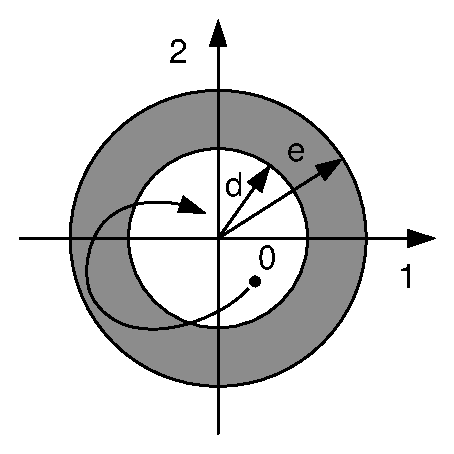
\includegraphics[width=.4 \linewidth,trim = 0cm 0cm 0cm 0cm]{3_delta_epsilon.eps}\label{fig:delta_epsilon}}
		%\psfrag{V}[rb][rb][1.]{$\frac{\partial}{\partial \bs x} V(\bs x)$}
		\hspace{.5cm}
		\psfrag{f}[cc][cc][1.]{$\bs f(\bs x)$}
		\psfrag{V}[cc][cc][1.]{$\frac{\partial}{\partial \bs x} V(\bs x)$}
		\psfrag{C}[tl][tl][1.]{$V(\bs x)\!=\!\text{const.}$}
		\subfigure[Lyapunov-Funktion]{
		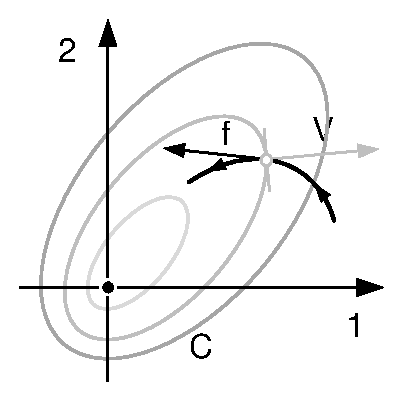
\includegraphics[width=.4 \linewidth,trim = 0cm 0cm 0cm 0cm]{3_Lyap_Funktion.eps}\label{fig:Lyap_Funktion}} 
	\caption[Veranschaulichung von Stabilitätsdefinition und -kriterium]{Veranschaulichung von Stabilitätsdefinition und -kriterium \cite{khalil2002nonlinear}}
	\label{fig:3_delta_epsilon}
\end{figure}

\begin{mydef}
Der stationäre Punkt $\bs x_s = \bs 0$ des autonomen Systems
	$ \dot {\bs x} = \bs f(\bs x) $
ist \emph{stabil} im Sinne von Lyapunov, wenn für jedes (noch so kleine) $\varepsilon > 0$ ein $\delta > 0$ %$\delta(\varepsilon)$ 
existiert, sodass %für jedes $\bs x_0 \in \mathcal X$
\begin{align*}
	\|\bs x_0 \| < \delta \Rightarrow \| \bs x(t)\| < \varepsilon, \forall t \geq 0 \;.
\end{align*}
Gilt zudem $\lim_{t\rightarrow \infty} \bs x(t)= \bs 0, \forall \bs x(0)\in \Omega$, so ist das System auf dem Gebiet $\Omega\in\mathbb R^n$ \emph{asymptotisch stabil}.
% S. https://www.kirp.chtf.stuba.sk/pc11/data/workshops/mpc/MPC_PC11_Lecture1.pdf -> S. 21
\end{mydef}

Für die Stabilitätsuntersuchung nichtlinearer Systeme, und hierzu zählt auch der modellprädiktive Regelkreis aufgrund seines aufwändigen Rückführungsgesetzes, eignet sich die sog.\ \emph{direkte Methode von Lyapunov} \cite{khalil2002nonlinear}:

\begin{satz} \label{theo:lyapunovstab}
Es sei $\mathcal D \subseteq\mathbb R^n$ eine offene Umgebung von $\bs x_s = \bs 0$. Existiert eine Funktion $V(\bs x):\mathcal D \rightarrow \mathbb R$, sodass %für $V(\bs x)$ auf $\mathcal D$ 
\begin{subequations}
\begin{align}
	V(\bs 0) &= 0; \quad \,\, V(\bs x) > 0, \,\, \forall \bs x \in \mathcal D \setminus\{\bs 0\} \label{equ:lyap_V}\\
%\end{align*}
%und
%\begin{align*}
	\dot V(\bs x) &= \frac{\partial }{\partial \bs x} V(\bs x)\bs f(\bs x) \leq - \alpha(\bs x), \,\, \forall \bs x \in \mathcal D \setminus\{\bs 0\} \, , \label{equ:lyap_V_dot}
\end{align}
\end{subequations}
wobei es sich bei $\alpha : \mathbb R^n \rightarrow \mathbb R$ um eine stetige positiv definite Funktion handelt, dann ist $\bs x_s=\bs 0$ auf $\mathcal D$ asymptotisch stabil, und $V(\bs x)$ wird Lyapunov-Funktion genannt.
\end{satz}
% abgewandelt aus
% MPC-Book

Bei der skalaren Lyapunov-Funktion $V(\bs x)$  handelt es sich um eine Energiefunktion im erweiterten Sinne: Sie ist nur Null im Ursprung, sonst positiv, s.\ \eqref{equ:lyap_V}, und muss über der Zeit stets abnehmen bis der Ursprung erreicht ist, s.\ \eqref{equ:lyap_V_dot}. %, damit $\dot{\bs x} = \bs f(\bs x)$ stabil ist. 
Die Existenz einer solchen Energiefunktion ist dann hinreichend dafür, dass $\bs x_s = \bs 0$ stabil im Sinne von Lyapunov ist, s.\ \zB \cite{khalil2002nonlinear}.
Zur Interpretation von \eqref{equ:lyap_V_dot} sei Abb.\,\ref{fig:Lyap_Funktion} betrachtet, worin die Höhenlinien von $V(\bs x)$ in unterschiedlichen Grautönen dargestellt sind. \\
Bei Anwendung des Stabilitätskriteriums auf Regelkreise werden $V(\bs x)$ als \emph{Control-Lyapunov-Funktion} (CLF) und die Rückführung  $\bs r(\bs x)$ als \emph{CLF-Reglergesetz} bezeichnet.

Das Stabilitätskriterium wird nun auf den zuvor durch die lineare ACC-Zustandsregelung \eqref{equ:lqr} geschlossenen Regelkreis angewandt, wobei die Ergebnisse ebenfalls für den späteren Entwurf einer leistungsstarken modellprädiktiven Regelung von Interesse sind. Die Zustandsrückführung wird nämlich optimal im Sinne eines LQR-Entwurfs \cite{lunze2012regelungstechnik} ausgelegt, der kurz erläutert werden soll.
\begin{mydef}
Ein sog.\ \emph{Linear Quadratic Regulator}\index{Linear Quadratic Regulator} (LQR) minimiert für ein lineares, zeitinvariantes System 
\begin{align}
 \dot{\bs x} = \bs A \bs x + \bs B \bs u, \quad \bs x(t) \in \mathbb R^n, \bs u(t) \in \mathbb R^m \label{equ:lq_problem_f}
\end{align}
das Kostenfunktional 
\begin{align*}
 J = \int_{t_0}^{\infty} [\bs x^\T \bs Q \bs x + \bs u^\T \bs R \bs u ]\,{\rm d} t \;. %\label{equ:lq_problem_J}
\end{align*}
\end{mydef}
Es wird hierbei auf den \emph{unendlichen} Optimierungshorizont hingewiesen. 
Der Einfachheit halber seien beide symmetrischen Wichtungsmatrizen $\bs Q=\bs Q^\T$ und $\bs R=\bs R^\T$ wie im ACC-Beispiel positiv definit\footnote{
Falls der allgemeine Fall einer positiv semidefiniten Matrix $\bs Q$ betrachtet werden soll, so ist der nachfolgende Stabilitätsbeweis für asymptotische Stabilität etwas aufwändiger.}. Es gilt folgender Satz \cite{graichen2014SkriptOpt}:
%
\begin{satz} \label{theo:lqr_stab}
Falls $\bs Q$ und $\bs R$ symmetrisch und positiv definit sowie $(\bs A,\bs B)$ stabilisierbar und $(\bs A,\bs M)$ mit $\bs Q = \bs M^\T \bs M$ entdeckbar sind, dann lautet das optimale Rückführgesetz
\begin{align}
\bs u(t) = \bs r(\bs x(t)) = -\bs R^{-1} \bs B^\T \bs P \, \bs x(t) = -\bs K_\text{LQR} \,\bs x(t) \;,   \label{equ:riccati_alg_u}
\end{align}
wobei $\bs P$ die eindeutige, symmetrische, positiv semidefinite Lösung der algebraischen Matrix-Riccati-Gleichung 
\begin{align}
\bs P \bs B \bs R^{-1} \bs B^T \bs P - \bs P \bs A - \bs A^T \bs P - \bs Q = \bs 0 \label{equ:riccati_alg}
\end{align}
darstellt. Die Ruhelage $\bs x_s = \bs 0$ des hierdurch geschlossenen Regelkreises ist asymptotisch stabil. \\
\end{satz}
Für die Herleitung von \eqref{equ:riccati_alg_u} und \eqref{equ:riccati_alg} wird auf Abschn.\,\ref{sec:riccati_dgl} verwiesen. Auch ohne sie kann auf Basis von Satz~\ref{theo:lyapunovstab} bereits die behauptete Stabilität gezeigt werden:

Mit dem Lyapunov-Funktionskandidaten
\begin{align}
	V(\bs x) = \bs x^\T \bs P \bs x \label{equ:lyap_lqr}
\end{align}
ergibt sich
\begin{align*}
	\dot V(\bs x) &= \dot{\bs x}^\T \bs P \bs x + \bs x^\T \bs P \dot{\bs x} \\
	&= [\bs x^\T \bs A^\T + \bs u^\T \bs B^\T]\bs P \bs x + \bs x^\T \bs P[\bs A \bs x + \bs B \bs u]
\end{align*}
und mit \eqref{equ:riccati_alg_u} und \eqref{equ:riccati_alg} gilt damit
\begin{align}
\nonumber
	\dot V(\bs x) &= \bs x^\T \bs A^\T \bs P \bs x  -\bs x^\T \bs P \bs B \bs R^{-1} \bs B^\T
	\bs P \bs x + \bs x^\T \bs P \bs A \bs x - \bs x^\T \bs P \bs B \bs R^{-1} \bs B^\T \bs P \bs x \\
\nonumber
	&= 	\bs x^\T [ \underbrace{\bs A^\T \bs P  -\bs P \bs B \bs R^{-1} \bs B^\T
	\bs P + \bs P \bs A}_{-\bs Q}] \bs x - \bs x^\T\bs P \bs B \bs R^{-1} \bs B^\T \bs P \bs x \\
	&= \underbrace{-\bs x^\T \bs Q \bs x}_{\leq 0} \quad \underbrace{- \bs x^\T \bs P \bs B \bs R^{-1} \bs B^\T \bs P \bs x}_{\leq 0} \quad \leq 0\;. \label{equ:V_dot_alg} 
\end{align}
Damit ist der Regelkreis auf $\mathbb R^n$ asymptotisch stabil.

Wird der ACC-Zustandsregler \eqref{equ:riccati_alg_u} auf Basis der Wichtungsmatrizen $\bs Q_\text{acc}$ und $R_\text{acc}$ in \eqref{equ:acc_integral} entsprechend Satz~\ref{theo:lqr_stab} entworfen, dann stabilisiert er asymptotisch die Ruhelage $\bs x_s = \bs 0$ "`per Design"'. Eine gesonderte Stabilitätsuntersuchung des Regelkreises, etwa durch Betrachtung dessen Pole, ist überflüssig. 
Wie in Abschn.\,\ref{sec:invariantSets} bereits dargelegt, reduziert sich das Einzugsgebiet $\mathcal D$ jedoch durch die Ungleichungsnebenbedingungen auf die maximal positiv invariante Menge $\mathcal{O}_\infty^{\text{\tiny LQR}}$.  

Die Lyapunov-Funktion \eqref{equ:lyap_lqr} kann anschaulich interpretiert werden, denn sie stellt die optimale Kostenfunktion $J^\ast(\bs x)$ dar. Auch die MPC-Schemata basieren auf den Kosten $J^\ast(\bs x)$ als Lyapunov-Funktion, um eine Stabilitätsgarantie aussprechen zu können.

% http://www.acin.tuwien.ac.at/fileadmin/cds/lehre/rsys/Archiv/Skriptum_Regelungssysteme_SS2011.pdf S.49

% 2) Wichtigstes Standardherangehen aus Regelungstechnik, konstruktiv, sodass MPC besser wird
% 3) Schwierigkeiten bei zeitvarianten Nebenbedingungen und gar bei zeitveränderlicher Umgebung

% Wichtige Punkte:
% - Als Systemeingang darf nicht u herangezogen werden, sondern die zu optimierenden Parameter wg. Approximation
% - Ausblick darauf, dass Optimierung nicht ganz abgeschlossen werden muss, um stabil zu sein, solange die Lyapunov-Funktion weiter abnimmt (Suboptimale Regelung)
% Es existiert immer ein hinreichend langer Horizont, sodass das System stabil ist. (gilt sicherlich nicht für zeitinvariante Probleme)

% Zu diskutierende Thesen: 
% Maximale control-invariante Menge (C_inf) = inv(ICS)  ?
% Zielmenge C_inf reicht nicht für persistent feasibility (anhaltende Realisierbarkeit) ? Begründung: Nur weil es eine Lösung gibt, heißt das nicht, dass ein Algorithmus, der auf einem endlichen Horizont optimiert, diese (in zeitlich aufeinanderfolgenden Schritten) findet.
% Was bringt mir dann die ICS-Menge?
% Was kann für zeitvariante NB abgeleitet werden?

% TODO: Hinweis darauf, dass bei LQ-Problemen sich Quadratisches Programm ergibt, das nicht numerisch approximiert werden muss und in einem Schritt gelöst werden kann.




% Vereinfachungen: Zeitvariante NB ändern sich nicht von Problem zu problem. 
% Was kann schief gehen: no feasibiltiy -> plötzlich keine Kollisionsfreie Traj, no stability: system schwing sich auf und nichtmodellierte Dynamiken werden angesprochen, sodass das System von der Straße abkommt.
%H. Chen und F. Allgower. A quasi-infinite horizon nonlinear model predictive control scheme with guaranteed stability. Automatica, 34(10):1205{1217, 1998.

% Kurze übersicht, auch invarianzregelung: https://www.kirp.chtf.stuba.sk/pc11/data/workshops/mpc/MPC_PC11_Lecture1.pdf

%Für einen endlich langen Optimierungshorizont muss der Endzustand in einer Invarianten Menge liegen, für die ein invarianz-induzierter Regler existiert, dessen Kosten auf einem unendlichlangen Horizont in geschlossener Form dargestllt werden kann. --> Lierfert Endbedingung und Enkosten, Regler wird aber nie verwendet!



%\subsection{Unendlicher Optimierungshorizont} \label{sec:infinit_horizon_mpc}
% es gibt eine obere schranke für den optimierungshorizont für die stabilität garantiert ist. Eher für die Simulation interessant. Erweiterung für zielmenge und endkosten aber für fahrzeuganwendung nicht tragisch, da problem nur unwesentlich komplizierter wird -> nächster Abschnitt

%If problem is feasible, the closed loop trajectories will be always feasible, If the cost is finite, then states and inputs will converge asymptotically to the origin [Folien Morari 5-30]
\subsection{MPC-Schema mit Garantien} %Endlicher Optimierungshorizont mit Zielregion} \label{sec:finite_horizon_mpc}
% Stabilitätsnachweis über Endzustand nicht möglich, da ggf. Endzustand nicht frei
% Optimalsteuerungsproblem definieren
% Fahrzeugmodelle + Ungebung -> gütekriterium + nebenbediunng
% Erklärung Lyapunov-Stabilität
% Trajektorienplanung für Fahrzeug: Optimierung auf endlichem Horizont ->
% Stabilität
Ein sehr weit verbreiteter MPC-Ansatz, der sich gut mit den Anforderungen der Fahrerassistenz vereinbaren lässt, basiert darauf, durch Vorgabe bestimmter Endkosten $V$ und einer Zielregion $\mathcal X_f$
%\begin{align*}
 %\bar{\bs x}(\tau_f) &\in \mathcal X_f; & \quad \tau_f &= t_k + T
%\end{align*}
für den Endzustand $\bar{\bs x}(t_k + T)$ die rekursive Lösbarkeit und Stabilität sicherzustellen. 
%Introduce terminal cost and constraints to explicitly ensure stability and feasibility:!
%https://www.kirp.chtf.stuba.sk/pc11/data/workshops/mpc/MPC_PC11_Lecture1.pdf
%
Für ein zeitinvariantes Problem stellt sich dann das schritthaltend zu lösende Optimalsteuerungsproblem als
\begin{subequations} \label{equ:mpc_problem_zeitinvariant}
\begin{align}
	\underset{\bar{\bs{u}}(\cdot)}{\text{minimiere}}  \quad & J(\bs x(t_k), \bar{\bs u}) =%J(\bs{\phi}(t,\bar{\bs{u}}),\bs{\psi}(t,\bar{\bs{u}}),t)) = 
	\int_{t_k}^{t_k+T} \!\!l(\bar{\bs x}(\tau), \bar{\bs u}(\tau))\,{\rm d} \tau\,\,+\,\, V(\bar{\bs{x}}(t_k+T)) \label{equ:mpc_funktional_inv}\\
	\text{u.B.v.} \quad &\dot{\bar{\bs{x}}}(\tau) = \bs{f}(\bar{\bs{x}}(\tau),\bar{\bs{u}}(\tau)), \quad \bar{\bs{x}}(t_k) = \bs{x}(t_k) \label{equ:mpc_system_inv}\\
	& \bar{\bs{x}}(\tau) \in \mathcal X, \quad \bar{\bs{u}}(\tau) \in \mathcal U, \quad \forall \tau \in[t_k, t_k + T] \label{equ:mpc_unb_Xf} \\
	& \bar{\bs x}(t_k + T)  \in \mathcal X_f%, \quad  \bar{\bs x}_f = \bar{\bs x}(t_k + T) \bar{\bs{x}}_f
\end{align} 
\end{subequations}
dar.

Der folgende Satz macht, unter recht milden Zusatzannahmen \cite{graichen2014SkriptOpt, gruene2011nonlinear}, eine Aussage darüber, wann \eqref{equ:mpc_problem_zeitinvariant} rekursiv lösbar und der modellprädiktive Regelkreis stabil ist:
\begin{satz}\label{theo:mpc_zielmenge}
Die Menge $\mathcal X_0 \subseteq \mathcal X \subseteq \mathbb R^n$ bezeichne die nichtleere Menge aller Anfangsbedingungen $\bs x(t_k)$, für die \eqref{equ:mpc_problem_zeitinvariant} lösbar ist.
Weiter existiert eine kompakte nichtleere Menge $\mathcal X_f=\{ \bs x \in \mathbb R^n : V(\bs x) \leq \beta \} \subseteq \mathcal X_0$ mit $\beta < 0$ und ein lokales Rückführgesetz $\bs u = \bs r(\bs x)\in \mathcal U$ für alle $\bs x \in \mathcal X_f$, sodass
\begin{align}
	\frac{\partial V}{\partial \bs x} \bs f(\bs x, \bs r(\bs x)) \leq -l(\bs x, \bs r(\bs x))  \quad \forall \bs x \in \mathcal X_f \;. \label{equ:mpc_control_lyapunov_ungl}
\end{align}
Dann ist der Ursprung des geregelten Systems asymptotisch stabil und $\mathcal X_0$ stellt den Einzugsbereich dar, auf dem rekursive Lösbarkeit gegeben ist. 
\end{satz}
Die Ungleichung \eqref{equ:mpc_control_lyapunov_ungl} fordert die Existenz eines Rückführgesetzes $\bs r(\bs x)$ auf $\mathcal X_f$, sodass entlang einer darüber geregelten Trajektorie die Zielkosten $V$ mindestens genauso schnell kleiner werden wie die negativen Integralkosten im Gütefunktional. Dann gilt nämlich, s.\ Beweis-Skizze in \ref{app:mpc_zielregion}, dass die optimalen Kosten $J^\ast$ über zwei aufeinanderfolgende Schritte $t_k$ und $t_k\!+\! \Delta t$ schneller abnehmen, als im Falle der Optimierung über einen unendlichen Horizont, was mit den optimalen Kosten $J^\ast$ als Lyapunov-Funktion asymptotische Stabilität garantiert. 
Hierbei ist die rekursive Lösbarkeit anschaulich dadurch sichergestellt, dass es im ersten Schritt auf $\mathcal X_0$ definitionsgemäß eine Lösung in die "`sichere"' positiv invariante Menge hinein gibt, der in jedem darauffolgenden Schritt gefolgt werden kann. \\
Ganz allgemein gesprochen stellt \eqref{equ:mpc_control_lyapunov_ungl} eine \emph{Control-Lyapunov-Ungleichung} dar \cite{gruene2011nonlinear, khalil2002nonlinear, graichen2014SkriptOpt}. An dieser Stelle sei darauf hingewiesen, dass das CLF-Reglergesetz $\bs r(\bs x)$ nicht implementiert wird, sondern lediglich die dazugehörige CLF als Endkostenterm $V(\bs x)$ dient.

Für ein lineares unbeschränktes System \eqref{equ:lq_problem_f} und quadratische Integralkosten $l(\bs x, \bs u) = \bs x^\T \bs Q \bs x + \bs u^\T \bs R \bs u$ ist bereits aus Abschn.\,\ref{sec:stabilität} ein entsprechendes CLF-Regelungsgesetz bekannt. Das
 Riccati-Rückführgesetz \eqref{equ:riccati_alg_u} mit der  Control-Lyapunov-Funktion \eqref{equ:lyap_lqr} erfüllt nämlich die Control-Lyapunov-Ungleichung \eqref{equ:mpc_control_lyapunov_ungl} in Gleichheit für alle $\bs x\in \mathbb R^n$:
%
\begin{align*}
\nonumber
l(\bs x, \bs r(\bs x))
	&= \bs x^\T \bs Q \bs x + \bs u^\T \bs R \bs u \\
	&= \bs x^\T \bs Q \bs x + [\bs R^{-1} \bs B^\T \bs P \bs x]^\T \bs R \bs R^{-1} \bs B^\T \bs P \bs x\\
	&= \bs x^\T \bs Q \bs x + \bs x^\T \bs P \bs B \bs R^{-1} \bs B^\T \bs P \bs x \\
	&\stackrel{\eqref{equ:V_dot_alg}}{=} - \frac{\partial V}{\partial \bs x} \bs f(\bs x, \bs r(\bs x))
\end{align*}

%\begin{align*}
%\nonumber
	%\frac{\partial V}{\partial \bs x} \bs f(\bs x, & \bs r(\bs x)) + l(\bs x, \bs r(\bs x)) = \\
	%&= -\bs x^\T \bs Q \bs x - \bs x^\T \bs P \bs B \bs R^{-1} \bs B^\T \bs P \bs x + \bs x^\T \bs Q \bs x + \bs u^\T \bs R \bs u \\
	%&= - \bs x^\T \bs P \bs B \bs R^{-1} \bs B^\T \bs P \bs x + [\bs R^{-1} \bs B^\T \bs P \bs x]^\T \bs R \bs R^{-1} \bs B^\T \bs P \bs x\\
	%&= 0
%\end{align*}

Zurückkehrend auf das ACC-Problem mit Ungleichungsbeschränkungen sichert damit Satz~\ref{theo:mpc_zielmenge} rekursive Lösbarkeit und asymptotische Stabilität, wenn im MPC-Reglergesetz \eqref{equ:mpc_problem_zeitinvariant}
\begin{align*}
	\mathcal X_f &= \mathcal O_\infty^{\text{\tiny LQR}} \\
	V(\bar{\bs x}_f) &= \bar{\bs x}_f^\T \bs P_\text{acc} \bar{\bs x}_f \quad \text{mit}\quad \bar{\bs x}_f = \bar{\bs x}(t_k + T) 
\end{align*}
gewählt wird, also die Zielregion mit der aus Abschn.\,\ref{sec:invariantSets} bekannten maximal positiv invarianten Menge des LQR-geregelten Systems übereinstimmt und
$\bs P_\text{acc}$ aus \eqref{equ:riccati_alg} mit den Wichtungsfaktoren $\bs Q_\text{acc}$ und $R_\text{acc}$ bestimmt wird.

Bei entsprechender Modifikation des zuvor vereinfacht entworfenen MPC-Reglers stellt sich der geschlossene Regelkreis ganz anders dar.
Zur Beurteilung sei erneut Abb.\,\ref{fig:MPC_Konvergenz} betrachtet. Darin wird dessen maximale invariante Menge mit einem Optimierungshorizont von $T=\unit[0.5]{s}$ als $\mathcal{O}_\infty^{0.5}$ bezeichnet, die allerdings nicht so ohne Weiteres geschlossen dargestellt werden kann. Aufgrund der Lösbarkeits- und Stabilitätsgarantie gilt jedoch grundsätzlich
\begin{align*}
	\mathcal O_\infty = \mathcal X_0 \;. %\label{equ:o_e_x}
\end{align*} 
Damit kann durch Sampling über $\bs x_\text{samp}\in \mathcal X$ geprüft werden, ob $\bs x_\text{samp} \in \mathcal X_0$, also ob für den Anfangszustand $\bs x(t_k) = \bs x_\text{samp}$ das Optimierungsproblem in \eqref{equ:mpc_problem_zeitinvariant} eine Lösung besitzt. In Abb.\,\ref{fig:MPC_Konvergenz} wird nur bei einem positiven Ergebnis ein dunkelgraues Rechteck an der Stelle $\bs x_\text{samp}$ eingezeichnet. Wie zu erkennen ist, fällt $\mathcal{O}_\infty^{0.5}$ größer als $\mathcal{O}_\infty^{\text{\tiny LQR}}$ aus, was den numerischen Aufwand der MPC rechtfertigt. Je länger darüber hinaus der Optimierungshorizont $T$ gewählt wird, desto mehr Anfangszustände existieren, von denen die Zielregion $\mathcal X_f$ erreicht werden kann. 
Zum Vergleich ist für $T=\unit[1.0]{s}$ die maximale invariante Menge $\mathcal{O}_\infty^{1.0}$ über große, hellgraue, rechteckige Samples dargestellt.

Die Zeitsignale in Abb.\,\ref{fig:MPC_Signals} verdeutlichen weiter die MPC-Arbeitsweise. Der Unterschied zwischen der MPC-Regelung mit $T=\unit[1.0]{s}$ (in Schwarz) zum unendlichen Optimierungshorizont $T=\infty$ (in Grau) ist gering. Kennzeichnend für den MPC-Entwurf nach Satz~\ref{theo:mpc_zielmenge} ist das "`konservative"' Regelungsverhalten, das insbesondere aus dem Ruckverlauf $u(t)$ und dem Beschleunigungssignal $a_\text{ego}(t)$ ersichtlich ist. Um innerhalb des endlichen Optimierungshorizonts in den sicheren Zustand $\mathcal X_f$ zu gelangen, wird gegenüber dem unendlichen Optimierungshorizont ein erhöhter Stellaufwand und damit auch eine stärkere Bremsung "`einberechnet"' (dünne schwarze Linien). Im nächsten Optimierungsschritt steht jedoch weiterhin der gesamte Optimierungshorizont $T$ zur Erreichung von $\mathcal X_f$ zur Verfügung, obschon sich der Systemzustand ein gutes Stück auf die Zielregion zubewegt hat. 
Damit fällt der erforderliche Stellaufwand geringer aus als zuvor berechnet. Insgesamt 
darf somit bereits früher von der Vollbremsung abgelassen werden, ohne dass der Sicherheitsabstand zum Vorderfahrzeug unterschritten wird. I.\,Allg.\  kann sich für Sicherheits- und Komfortfunktionen das Optimierungsproblem immer zeitlich zuspitzen, sodass ein solches konservatives Verhalten nicht unbedingt von Nachteil ist.

An dieser Stelle kann zusammengefasst werden, dass die zyklische Optimierung auf einem endlichen Horizont nicht automatisch Stabilität und rekursive Lösbarkeit des geschlossenen Regelkreises impliziert. 
Weiter gestaltet sich die Lösbarkeits- und Stabilitätsanalyse des geschlossenen Regelkreises aufgrund des \iA nichtlinearen Prädiktivreglers äußerst schwierig. Aus dem Grund existieren MPC-Schemata, die durch die gezielte Vorgabe von Endbedingungen und -kosten den geschlossenen Regelkreis auf das "`Kommende"' vorbereiten, und damit trotz des endlichen Optimierungshorizonts die rekursive Lösbarkeit und Stabilität garantieren. Allen gemeinsam ist die Verwendung der optimalen Kosten $J^\ast(\bs x(t_k))$ als Lyapunov-Funktion, deren zeitliche Abnahme bekanntermaßen Stabilität garantiert.
Das vorgestellte MPC-Schema kombiniert hierfür die (numerische) Optimierung auf einem kurzen Horizont mit einem klassischen (offline entworfenen) Regler, der wiederum die Zielkosten und Endregion in der MPC bestimmt. Im Falle der LQ-Regelung kann dasselbe Optimierungskriterium zugrunde gelegt werden wie im MPC-Optimalsteuerungsproblem, sodass der MPC-Regler nicht nur stabil ist, sondern das Verhalten des unendlichen Optimierungshorizonts nachahmt\footnote{Dies ist der Grund dafür, dass der LQ-Regler die Ungleichung \eqref{equ:mpc_control_lyapunov_ungl} in Gleichheit erfüllt.}. Die Kosten im Optimalsteuergesetz stellen dann immer eine obere Abschätzung der optimalen Kosten des unendlichen Optimierungshorizonts dar, sodass in dem Zusammenhang auch der Begriff \emph{quasi-infinite horizon MPC} \cite{Findeisen2002} gebräuchlich ist.

\begin{figure}[ht]
	\centering
	% Generated using matlabfrag
% Version: v0.6.16
% Version Date: 04-Apr-2010
% Author: Zebb Prime
%
%% <text>
%
\providecommand\matlabtextA{\color[rgb]{0.000,0.000,0.000}\fontsize{10}{10}\selectfont\strut}%
\psfrag{022}[bc][bc]{\matlabtextA \xlabel}%
\psfrag{023}[tc][tc]{\matlabtextA \ylabelA}%
\psfrag{024}[tc][tc]{\matlabtextA \ylabelB}%
\psfrag{025}[tc][tc]{\matlabtextA \ylabelC}%
\psfrag{026}[tc][tc]{\matlabtextA \ylabelD}%
%
%% </text>
%
%% <xtick>
%
\def\matlabfragNegXTick{\mathord{\makebox[0pt][r]{$-$}}}
%
\psfrag{000}[ct][ct]{\matlabtextA $0$}%
\psfrag{001}[ct][ct]{\matlabtextA $0.5$}%
\psfrag{002}[ct][ct]{\matlabtextA $1$}%
\psfrag{003}[ct][ct]{\matlabtextA $1.5$}%
\psfrag{004}[ct][ct]{\matlabtextA $2$}%
\psfrag{005}[ct][ct]{\matlabtextA $2.5$}%
%
%% </xtick>
%
%% <ytick>
%
\psfrag{006}[rc][rc]{\matlabtextA $-40$}%
\psfrag{007}[rc][rc]{\matlabtextA $-20$}%
\psfrag{008}[rc][rc]{\matlabtextA $0$}%
\psfrag{009}[rc][rc]{\matlabtextA $20$}%
\psfrag{010}[rc][rc]{\matlabtextA $-10$}%
\psfrag{011}[rc][rc]{\matlabtextA $-5$}%
\psfrag{012}[rc][rc]{\matlabtextA $0$}%
\psfrag{013}[rc][rc]{\matlabtextA $5$}%
\psfrag{014}[rc][rc]{\matlabtextA $-10$}%
\psfrag{015}[rc][rc]{\matlabtextA $0$}%
\psfrag{016}[rc][rc]{\matlabtextA $10$}%
\psfrag{017}[rc][rc]{\matlabtextA $20$}%
\psfrag{018}[rc][rc]{\matlabtextA $-20$}%
\psfrag{019}[rc][rc]{\matlabtextA $-10$}%
\psfrag{020}[rc][rc]{\matlabtextA $0$}%
\psfrag{021}[rc][rc]{\matlabtextA $10$}%
%
%% </ytick>
	\renewcommand{\matlabtextA}{\scriptsize}	
	\def\xlabel{$t,\tau$ in $\unit{s}$}	
	\def\ylabelA{$u$ in $\unitfrac{m}{s^3}$}	
	\def\ylabelB{$a_\text{ego}$ in $\unitfrac{m}{s^2}$}		
	\def\ylabelC{$\Delta v$ in $\unitfrac{m}{s}$}	
	\def\ylabelD{$\Delta x$ in $\unit{m}$}		
  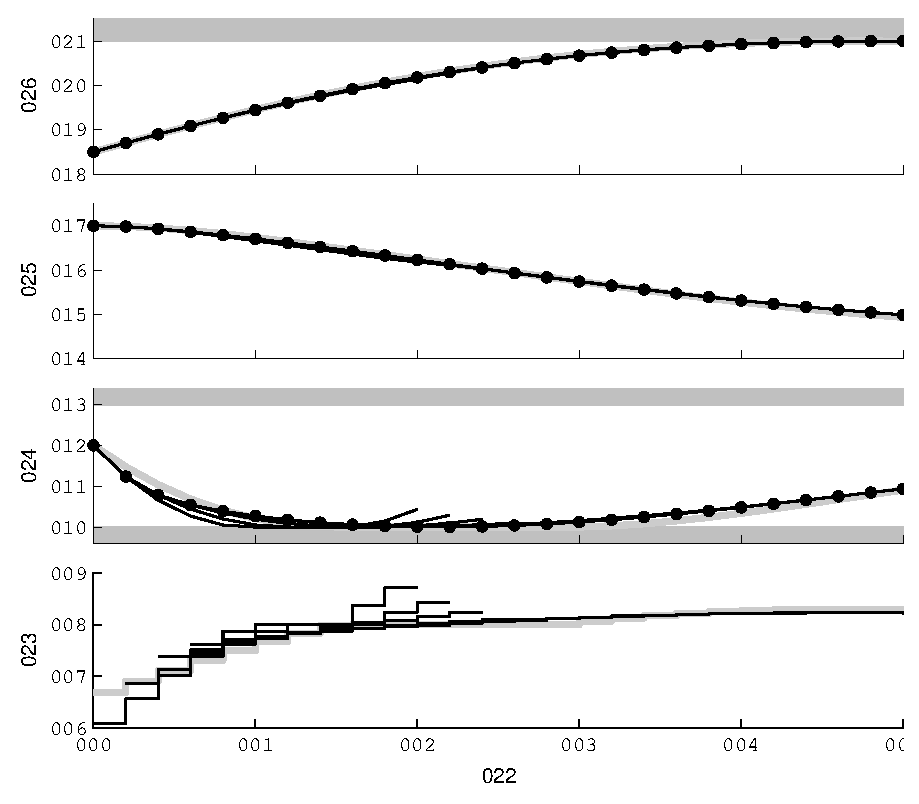
\includegraphics[width=.9 \linewidth,trim = 0cm 0cm 0cm 0cm]{3_MPC_Signals.eps}
    \caption[Trajektorienzeitverläufe der modellprädiktiven Regelkreise]{Zeitverläufe der Trajektorien der beiden modellprädiktiven Regelkreise; $T=\infty$ in Grau, $T=\unit[1.0]{s}$ in Schwarz; Ungleichungsnebenbedingungen repräsentiert durch graue Balken}
    \label{fig:MPC_Signals}
	\end{figure}
  




%\subsection{Parallelen zu Inevitable Collision States}
% - Keine Stabilitätsbetrachtung, sichert "`nur"' realisierbarkeit der Trajektorie
% - Keine Berücksichtigung weiterer NB?
% - Konstruktives Konzept? Eher nein, das ICS-Checker nicht gelöst

% Gütekritierium: If the cost is a kind of reward, as in investment planning or in most AI books, then maximization is preferred. [LaValle]
% Zur Seitenzahlreduktion: Nur Krümmungsregelung des Anhängers mit der Motivation, dass die überlagerte Optimierung erst noch behandelt wird, die der Mensch im Anhängerbeispiel übernimmt.

% Graicheninhalte:
% Lösen von Optimalsteuerungsproblem, Hinschreiben mit Tildegrößen oder so
% Prinzip MPC, Optimierung wird gelöst in jedem schritt

% \cite{allgower2004nonlinear}: 
% intuitive darstellung infinite horizont wie bei mir in der diss
% finiter horizont: endkosten müssen so ausgelegt werden, dass sie eine obere schranke für die ausstehenden kosten darstellen
% Unterscheidung zwischen nomineller stabilität und robustheit
%\cite{johansen2011introduction} wie allgower2004nonlinear, nur neuer

% Ideen
% Abprüfung der stabilität anhand von isolierten szenarien (z.B. isoliertes FAhrzeug)
% Echtzeitimplementierung in der Regelungstechnik versucht den Horizont so kurz zu halben wie möglich. Beim Fahrzeug auf Führungsebene ist das aber nicht möglich, da immer eine gewissen vorausschau erforderlich ist.
% Feasisbility / ics etc. ist nur sehr schwer zu berechnen / zeigen: deshalb heuristiken wie constant time gap control wichtig.
% modellidentifikation (wichtig sonst in der regelungstechnik) ist nicht wichtig auf führungsebene, wenn davon ausgegangen wird, dass krümmungen und beschleunigungen exakt umgesetzt werden.
% Dies ist auch der grund warum robustness auf führungsebene nicht so wichtig solange die unterlagerte regelung hinreichend gut ist. Kommentar bei robustheit hinzufügen, der auf robuste NMPC verweist, aber auch mit dem hinweis, dass robustheit hier mit unterlagerter regelung erreicht wird.



% Hier stabilisierung, auch durch überlagerte Optimierung
% Aus der Optimalität können stabilitätseigenschaften abgeleitet werden, weshalb im folgenden ein großer Wert auf optimierung gelegt wird.

% lavalle: 15.1.Lyapunov functions in planning
% Aber häufig keine Optimierung bis zum ziel möglich

% Bei stabilisierung: brockett1983asa zumindest erwähnen

%Dang übersicht über Einflussmöglichkeiten: Lenkung, Panzerbremse, Hinterradlenkung, torque vectoring
\newpage
\section{Robustheit\index{Robustheit} durch unterlagerte Regelungen}\label{sec:unterlagerteRegelung} \label{sec:sys_stab}
\zitat{Wennst den Baum siehst, in den du rein fährst, hast Untersteuern\index{Untersteuern}. \\ 
		Wennst ihn nur hörst, hast Übersteuern\index{Übersteuern}.}{Walter Röhrl}
%\subsection{Modellprädiktive Regelung im kaskadierten Regelkreis} 
Soll in die Manöverberechnung immer die neu erfasste Umfeldinformation einfließen, damit das Fahrerassistenzsystem schnell auf die Verkehrssituation reagiert, so hat die Trajektorienoptimierung permanent zu erfolgen. Entsprechend des vorhergehenden Abschnitts kann hierbei zusätzlich der aktuelle Systemzustand des Eigenfahrzeugs berücksichtigt werden. Gemäß Abschn.\,\ref{sec:stab_mpc} ist durch die entstehende Zustandsrückführung, zumindest theoretisch, eine vollständige Systemstabilisierung erzielbar. Die Analyse praktischer Anwendungen wie \cite{graichen_suboptimal, wahl2003ora, arnold2008mpt, schmidt2012hierarchischer} fördert jedoch zutage, dass der modellprädiktive Regelkreis in seiner reinen Form, bei der das optimierte Signal $\bs u(t)$ auch der tatsächlichen Streckenstellgröße entspricht (Steuerspannung, Bussignal etc.), nicht häufig zum Einsatz kommt. Stattdessen wird die Optimierung mit einer unterlagerten klassischen Regelung kombiniert. Die überlagerte modellprädiktive Regelung fungiert dann als sog.\ Führungsregler\index{Führungsregler}, dessen Ausgang dem unterlagerten Folgeregler als Referenz zugeführt wird und es entsteht eine Reglerkaskade\index{Kaskadenregelung}. Je nach Anzahl der unterlagerten Regelkreise generiert der Ausgang des unterlagerten Reglers die eigentliche Stellgröße oder wiederum das Referenzsignal für den nächsten unterlagerten Folgeregler\index{Folgereglung}. Auch das Elektronische Stabilitätsprogramm (ESP) (s.\ \zB \cite{handbuchFAS_Winner, liebemann2004safety, BHB2012_vanZanten_bremsanlage, vietinghoff2008nichtlineare, trachtler2005integrierte}) kann, ganz im Einklang mit dem modifizierten Drei-Ebenen-Modell in Abschn.\,\ref{sec:drei-ebenen-modell}, als unterlagerter Regler für den Fahrer als Trajektorienoptimierer angesehen werden, s.\ Abb.\,\ref{fig:ESP_Funktionsweise}.
%
\begin{figure}[h]
	\psfrag{U}[lc][lc][1.0]{Untersteuern\index{Untersteuern}}
	\psfrag{E}[lc][lc][1.0]{Übersteuern\index{Übersteuern}}
	\psfrag{B}[lc][lc][1.0]{Bremseingriff}
	\centering
  	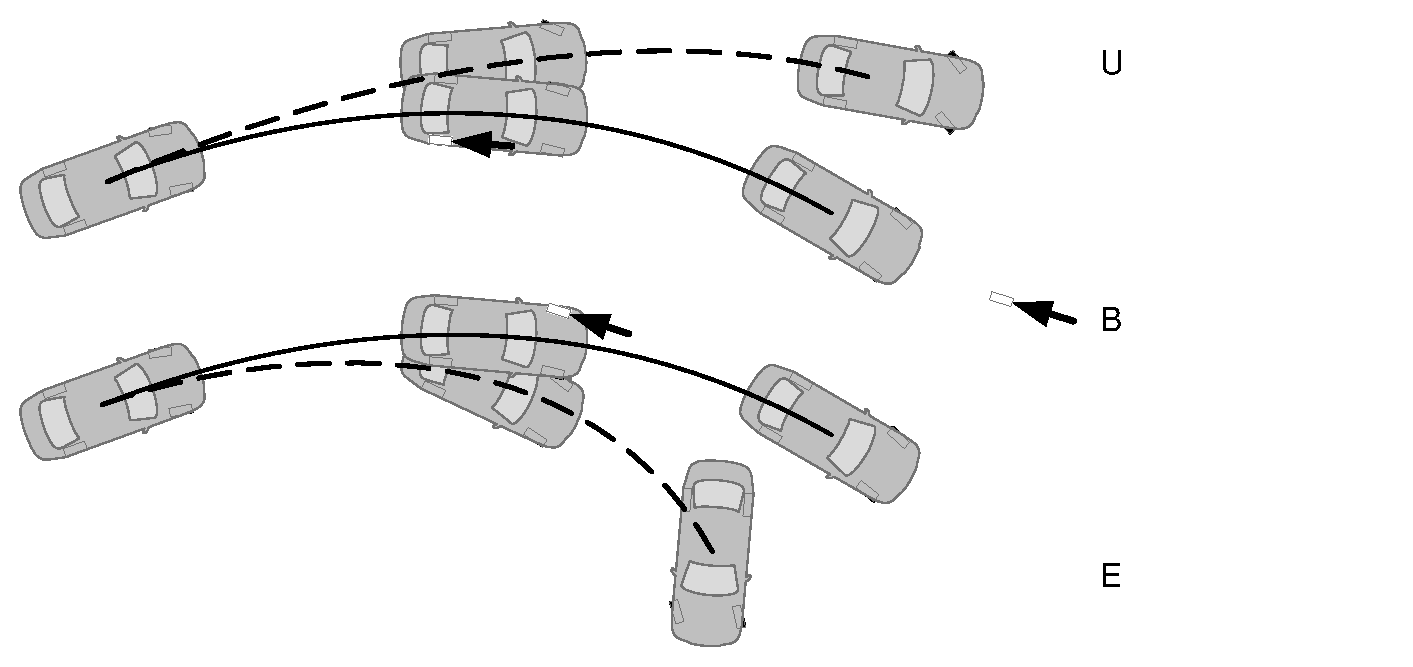
\includegraphics[width=1.05\textwidth,clip, trim = 0cm 0cm 0cm 0cm]{3_ESP_Funktionsweise.eps}
  	\caption[Funktionsweise vom ESP]{ESP sorgt dafür, dass sich das Fahrzeug auch in fahrphysikalischen Grenzsituationen sehr ähnlich zur gewohnten Dynamik der Normalfahrt verhält und damit der Mensch-Maschine-Regelkreis robust gegen Modellschwankungen und Störungen wird. Hierzu bremst das Fahrzeug einzelne Räder derart ab, dass sich das Fahrzeug möglichst ähnlich zu seinem linearen Einspurmodell verhält \cite{BHB2012_vanZanten_bremsanlage}.}
    \label{fig:ESP_Funktionsweise}
\end{figure} 


\subsection{Motivation unterlagerter Regelungen}
Aus der Praxis sind für die Kombination einer modellprädiktiven Regelung mit einer unterlagerten Folgeregelung folgende Hauptgründe zu nennen:

\textbf{Modellkomplexität:} \\
Die Wirkungsweise des klassischen Kaskadenregelkreises beruht darauf, dass der unterlagerte Regler eine Teilstreckendynamik stabilisiert und ihr zu Schnelligkeit verhilft, sodass sie im Entwurf des überlagerten Reglers vernachlässigt werden kann \cite{graf2003neue}. In gleicher Weise reduziert auch beim Entwurf der modellprädiktiven Regelung ein schneller unterlagerter Regler erheblich die Systemkomplexität des Prädiktionsmodells.

\textbf{Zykluszeiten und Übertragungslatenzen:} \\
Insbesondere die Überprüfung der Fahrtrajektorie auf Kollisionen mit dem Fahrzeugumfeld und die für bestimmte Optimierungsverfahren erforderliche numerische Simulation der Eigenfahrzeugdynamik beanspruchen einige Rechenzeit. %Dies verbietet bei vielen Optimierungsverfahren eine quasi-kontinuierliche\footnote{todo} Implementierung. 
Hinzu kommt, dass die Informationsübertragung zwischen Computer (das Steuergerät im Fall der Fahrerassistenz), Sensor und Aktor latenzbehaftet ist. Schnelle Streckendynamiken mit geringer Eigenstabilität werden damit nicht genügend rasch von der Optimierung beeinflusst. Ein unterlagerter Regler hingegen kann häufig direkt in der Aktorikelektronik integriert werden, wo ihm die Sensorinformation mit geringer Latenz zur Verfügung steht.

\textbf{Permanente Störungen und Modellfehler:} \\
Während impulsförmige Störungen bereits im nächsten Optimierungsschritt berücksichtigt werden können, leidet die Qualität des modellprädiktiven Regelkreises ganz erheblich unter permanenten Störungen und Modellfehlern\footnote{Beim Fahrzeug gehören dazu eine hängende Fahrbahn, Windeinflüsse, witterungsbedingte Reibwertänderungen und vor allem Vereinfachungen des komplexen Reifenkraftaufbaus.}. Da sich aufgrund der verschiedenartigen Einflussfaktoren eine genaue Störgrößenbeobachtung \cite{lunze2012regelungstechnik} bzw.\ Modelladaption \cite{kok95} oftmals sehr aufwändig gestaltet, stellt der Einsatz unterlagerter Regler eine häufig präferierte Alternative dar. Er sorgt dann dafür, dass sich die Dynamik der geregelten Teilstrecke trotz Störungen und Modellfehlern ähnlich dem Prädiktionsmodell verhält.

\textbf{Wiederverwendung unterlagerter Regelungen und Modularität:} \\
Die im Fahrzeug verbaute Aktorik (s.\ \abschn{sec:aktuatorik}) leistet bereits verlässlich ihren Dienst für verschiedene Stabilisierungssysteme wie ABS und ESP \cite{kiencke2005automotive, isermann2006frm}, s.\ Abb.\,\ref{fig:ESP_Funktionsweise}. Wie auch in anderen technischen Anwendungen wird hierbei vom Aktorhersteller bereits eine intensiv getestete und auf die jeweilige Hardware optimierte Regelung angeboten, die 1:1 in eine überlagerte modellprädiktive Regelung eingebettet werden kann. Neben der damit verbundenen Arbeitsersparnis wird, aufgrund der Einführung einer abstrahierten Schnittstelle, für den überlagerten Regelkreis eine weitgehende Unabhängigkeit von den Parametern der unterlagert stabilisierten Teilstrecke (Aktorik, Fahrzeugteildynamik etc.) erreicht. Die damit verbundene Steigerung von Flexibilität und Modularität ist in Anbetracht breiter Produktpaletten (Fahrzeugtypen und Sonderausstattungen) zur heutigen Zeit unverzichtbar \cite{rathgeber_ecc2014}.

%Angesichts der offensichtlichen Tragweite des Zusammenspiels von optimaler und klassischer Regelung für die Fahrerassistenz (bei gleichzeitigem Mangel an entsprechender Literatur) wird die Thematik in \abschn{sec:sys_stab} systematisiert und weiter vertieft.


% Robustheitsbetrachtungen sehr aufwändig. Als zweckmäßig haben sich aber unterlagerte regelungen herausgestellt, die die Fahrzeugbewegung umsetzen. Dann bleibt noch nichtlineare kinematik (Ebene Bewegung) übrig, die keine Parameterschwankungen unterliegt.
%\section{Systematische Betrachtungsweise der Stabilisierungsaufgabe} % oder so..

Da die Realisierung von unterlagerten modellprädiktiven Regelkreisen keinesfalls trivial ist, werden im Folgenden die möglichen Umsetzungsvarianten systematisiert. Hierbei sei vereinfachend angenommen, dass beim unterlagerten Regelkreis ein einzelner statischer, d.h.\ zustandsfreier, Regler eingesetzt wird. Eine Übertragung der Ergebnisse auf dynamische oder mehrfach-kaskadierte Regler ist jedoch ohne Einschränkung möglich.
Die Einteilung der kaskadierten Regelungsstruktur erfolgt nach dem asymptotischen Verhalten der unterlagerten Folgeregelungen.

\subsection{Nicht-asymptotische Folgeregelung} \label{sec:nichtasymptotischeFolgeregelung}
Aufgrund des Tiefpasscharakters der Aktorik ist in der Ein-Freiheitsgrad-Struktur, d.h.\ ohne Vorsteuerung, ein asymptotischer Folgeregler nicht realisierbar. Dennoch kann eine nicht-asymptotische Folgeregelung, insbesondere aufgrund der mit ihr verbundenen Einfachheit, in vielen Situationen einen wertvollen Beitrag liefern.
Die Integration des unterlagerten Folgereglers in den überlagerten modellprädiktiven Regelkreis ist denkbar einfach. Hierzu sei Abb.\,\ref{fig:KR_Unterlagerte_Stabilisierung} betrachtet, aus der unmittelbar ersichtlich wird, dass die überlagerte Optimierung (MPC) den durch die unterlagerte Rückführung $\bs x_1$ geschlossenen Regelkreis als neue Gesamtstreckendynamik $\Sigma'$ aufzufassen hat. Das Führungssignal des unterlagerten Folgereglers ist hierbei als neuer Systemeingang zu betrachten, und damit die Stellgröße $\tilde{\bs u}$ aus Optimalsteuersicht der MPC. \\
Bei geeigneter Auslegung der Folgeregelung weist das neue System $\Sigma'$ gegenüber der ursprünglichen Strecke $\Sigma$ ein gutmütigeres Verhalten auf, sodass der überlagerte modellprädiktive Regelkreis mit einer längeren Zykluszeit auskommt, da die Strecke während eines Optimierungszyklus durch die unterlagerte Stabilisierung nicht "`wegläuft"'. Darüber hinaus erleichtert die veränderte Streckendynamik die für bestimmte numerische Optimierungsverfahren erforderliche Simulation von $\Sigma'$, s.\ Abschn.\,\ref{sec:direkte_mehrfach_schiessverfahren}, oder sie weist durch die Rückführung so schnelle Teildynamiken auf, dass sie aus MPC-Sicht vernachlässigt werden können. \\
Falls keine Teildynamiken vernachlässigt werden können und die Rückkopplung im modellprädiktiven Regelkreis ohnehin häufig erfolgt, so kann der unterlagerten Regelung \iA keine robustheitssteigernde Wirkung in Bezug auf Modellfehler und Störungen zugeschrieben werden. Der Grund hierfür ist, dass es sich beim unterlagerten Regelkreis in der Rückkopplung um dasselbe $\bs x_1$ handelt wie in die modellprädiktive Regelung in $\bs x$ zurückgeführt wird. Anschaulich gesprochen invertiert damit die überlagerte Optimierung 1:1 die Folgeregelung im Modell $\Sigma'$, welche ja lediglich eine statische Abbildung von $\bs x_1$ und $\tilde{\bs u}$ auf $\bs u$ darstellt, sodass dort auch gleich $\bs u$ berechnet werden könnte.

\begin{figure}[h]
\centering
\newcommand{\smallsize}{.85}
		\psfrag{u}[cb][cb][1.]{$\bs u$}
		\psfrag{v}[cb][cb][1.]{$\tilde{\bs u}$}
		\psfrag{x}[cb][cb][1.]{$\bs x$}
		\psfrag{1}[cc][cc][1.]{$\Sigma$}
		\psfrag{m}[cb][cb][1.]{$\bs x_1$}
		\psfrag{g}[cb][cb][1.]{$\Sigma'$}
		\psfrag{c}[cc][cc][\smallsize]{\parbox[c]{7cm}{\begin{center}MPC\\ $\Sigma'$ \end{center}}}
				\psfrag{t}[cc][cc][\smallsize]{\parbox[c]{7cm}{\begin{center}Folge- \\ regelung \end{center}}}
	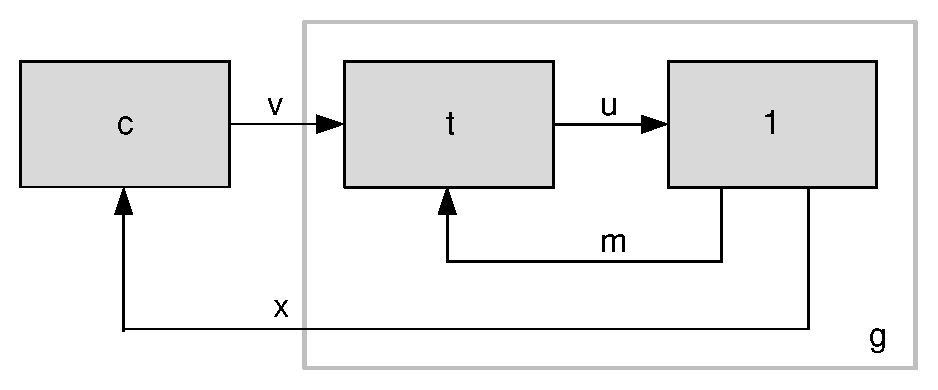
\includegraphics[width=.6\textwidth,clip, trim = 0cm 0cm 0cm 0cm]{2_KR_Unterlagerte_Stabilisierung.eps}
	\caption{Modellprädiktive Regelung mit unterlagerter Folgeregelung}
	\label{fig:KR_Unterlagerte_Stabilisierung}
\end{figure}

\subsection{Asymptotische Folgeregelung} \label{sec:asymptotische_folgeregelung}
Bevor nun die etwas aufwändigere Integration eines asymptotischen Folgereglers in den modellprädiktiven Regelkreis erläutert wird, soll als Vorstufe zunächst der Sonderfall betrachtet werden, in dem die Systemstellgröße $\bs u(t)$ aufgrund praktischer Anforderungen stetig verlaufen muss. Diese Herangehensweise ist erforderlich, wie im Beispiel der modellprädiktiven Abstandsregelung in Abschn.\,\ref{sec:mpc_acc}, wenn in der überlagerten Optimierung die Stellrate $\dot{\bs u}$ im Gütekriterium oder in den Nebenbedingungen (Stellratenbeschränkung) berücksichtigt werden muss. \\
Damit die Stetigkeitsbedingung an $\bs u$ erfüllt werden kann, muss in jedem Schritt die vorherige Stellgröße verfügbar sein, sodass die Aufgabe nur von einem dynamischen Regelkreis, der die vorherige Stellgröße als Zustand besitzt, erfüllt werden kann. Eine gleichermaßen einfache wie anschauliche Realisierung erfolgt entsprechend Abb.\,\ref{fig:KR_Integrator_Erweiterung} über die Systemerweiterung von $\Sigma$ um einen vorgelagerten Integrator, dessen Ausgang die Stellgröße $\bs u$ liefert. Gleichzeitig ist nun das Integral als Zustand $\bs z=\bs u$ des erweiterten Systems $\Sigma'$ aufzufassen und nebst $\bs x$ in die modellprädiktive Regelung zurückzuführen. Das dort zu lösende Optimalsteuerungsproblem hat nun das erweiterte System $\Sigma'$ zu berücksichtigen, da die Stellgröße $\tilde{\bs u}$ den Integratoreingang darstellt. Die Implementierung der Integratorerweiterung erfolgt durch numerische Integration von $\tilde{\bs u}(t)$.

\begin{figure}[h]
\centering
\newcommand{\smallsize}{.85}
	\psfrag{a}[cc][cc][\smallsize]{\parbox[c]{7cm}{\begin{center}MPC\\ $\Sigma'$ \end{center}}}
		\psfrag{i}[cc][cc][1.]{$\int$}
		\psfrag{u}[cb][cb][1.]{$\bs u$}
		\psfrag{v}[cb][cb][1.]{$\tilde{\bs u}$}
		\psfrag{z}[rb][rb][1.]{$\bs z\!=\!\bs u$}
		\psfrag{x}[cb][cb][1.]{$\bs x$}
		\psfrag{e}[br][br][1.]{$\Sigma'$}
		\psfrag{s}[cc][cc][1.]{$\Sigma$}
	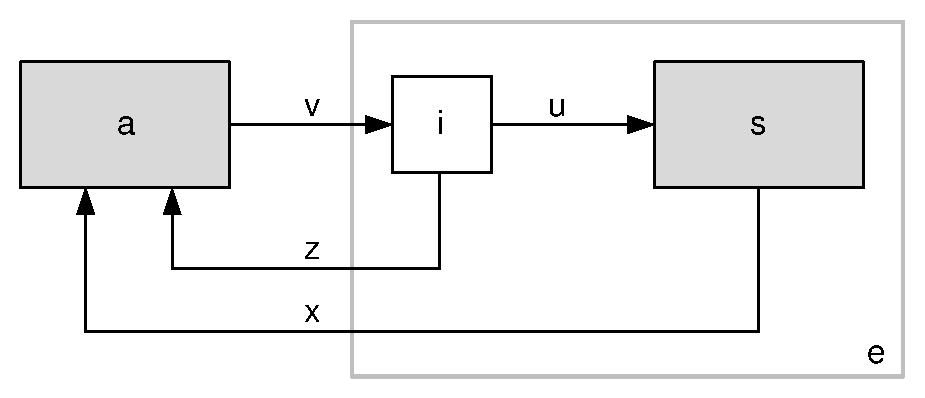
\includegraphics[width=.6\textwidth,clip, trim = 0cm 0cm 0cm 0cm]{2_KR_Integrator_Erweiterung.eps}
	\caption{Modellprädiktive Regelung mit Integratorerweiterung}
	\label{fig:KR_Integrator_Erweiterung}
\end{figure}

Für die Unterlagerung der modellprädiktiven Regelung mit einer asymptotischen Folgeregelung ist ähnlich zu verfahren. Der Grund hierfür ist, dass von einer Folgeregelung nur realisierbare (insbesondere hinreichend oft stetig differenzierbare) Referenzverläufe asymptotisch stabilisiert werden können. \\
Da die asymptotische Folgeregelungsaufgabe keinesfalls die gesamte Systemdynamik umfassen muss, erfolgt im ersten Schritt entsprechend Abb.\,\ref{fig:KR_Unterlagerte_Folgeregelung} eine Unterteilung der Strecke in das asymptotisch zu stabilisierende Teilsystem $\Sigma_1$ und ihre restliche Dynamik $\Sigma_2$. Im zweiten Schritt wird der Regelkreis um das System $\tilde \Sigma_1$ erweitert, das so gewählt werden muss, dass dessen Ausgang dem Folgeregler nur realisierbare Referenzverläufe generiert. Darüber hinaus muss es ein ähnliches Streckenverhalten wie $\Sigma_1$ aufweisen, damit sich dessen Zustände $\tilde {\bs x}_1$ nicht allzu sehr von $\bs x_1$ unterscheiden, da nur erstere im Optimierungskriterium Berücksichtigung finden (s.\ Rückführung $\tilde {\bs x}_1$ in Abb.\,\ref{fig:KR_Unterlagerte_Folgeregelung}). \\
Aufgabe der Folgeregelung ist es nun, das System $\Sigma_1$hinreichend genau mittels $\bs u$ zu stabilisieren (im Idealfall asymptotisch), sodass $\tilde {\bs w}(t) \approx \bs w(t)$, also der Systemausgang von $\Sigma_1$ hinreichend genau dem von $\tilde\Sigma_1$ folgt. Der modellprädiktive Regelkreis kann dann nämlich auf Basis der Verkettung von simuliertem Teilsystem $\tilde \Sigma_1$ und Reststrecke $\Sigma_2$ entworfen werden, deren jeweilige Systemzustände $\tilde {\bs x}_1$ und $\bs x_2$ wiederum in das Optimalsteuerungsproblem rückzuführen sind. \\
Neben den zuvor erwähnten Vorteilen der nicht-asymptotischen Folgeregelung wird zusätzlich Robustheit gegen permanente Störungen und Modellfehler im Teilsystem $\Sigma_1$ erlangt. Allerdings wird sie mit einer erhöhten Anfälligkeit auf Impulsstörungen desselben Teilsystems erkauft.
Schließlich spiegeln sich diese nicht in den in die Optimierung rückgeführten Systemgrößen $\tilde {\bs x}_1$ wider, sondern müssen %nicht auf $\tilde\Sigma_1$ wirken und damit 
vom Folgeregler ausgeregelt werden.
%
\begin{figure}[h]
\centering
\newcommand{\smallsize}{.85}
			\psfrag{b}[cc][cc][\smallsize]{\parbox[c]{7cm}{\begin{center}MPC\\ $\tilde\Sigma_1 \Sigma_2$ \end{center}}}
		\psfrag{u}[cb][cb][1.]{$\bs u$}
		\psfrag{v}[cb][cb][1.]{$\tilde{\bs u}$}
		\psfrag{x}[cb][cb][1.]{$\bs x$}
		\psfrag{0}[cc][cc][1.]{$\tilde \Sigma_1$}
		\psfrag{r}[cc][cc][\smallsize]{\parbox[c]{7cm}{\begin{center}asympt.\ \\ Folgeregler  \end{center}}}
		\psfrag{1}[cc][cc][1.]{$\Sigma_1$}
		\psfrag{2}[cc][cc][1.]{$\Sigma_2$}
		\psfrag{w}[cb][cb][1.]{$\tilde{\bs w}$}
		\psfrag{n}[cb][cb][1.]{$\bs w$}
		\psfrag{m}[cb][cb][1.]{$\bs x_1$}
		\psfrag{k}[cb][cb][1.]{$\bs x_2$}
		\psfrag{l}[cb][cb][1.]{$\tilde {\bs x}_1$}
		\psfrag{f}[br][br][1.]{$\approx\!\bs 1$}
	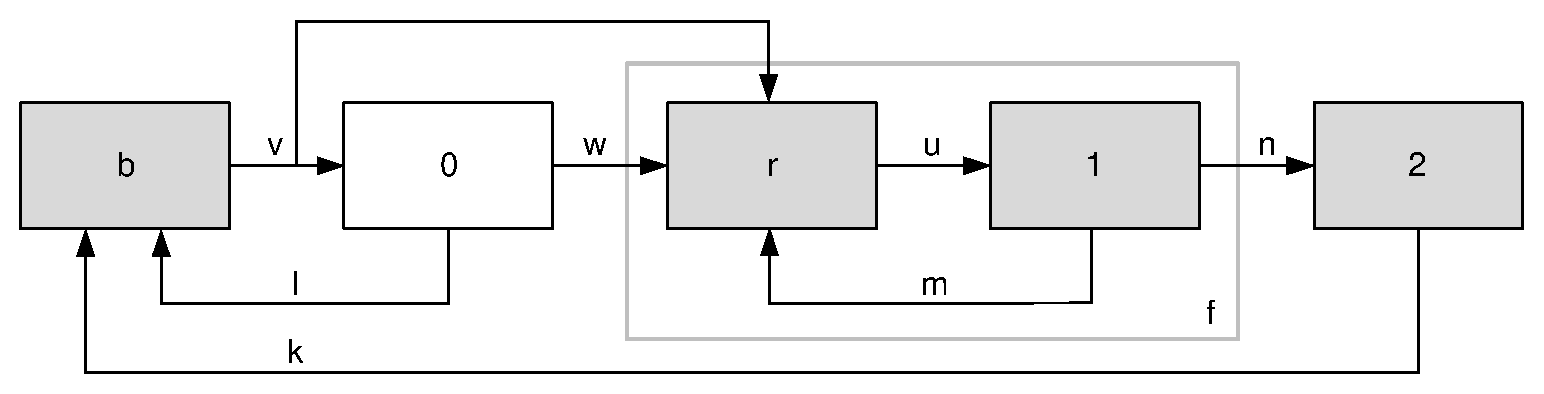
\includegraphics[width=1\textwidth,clip, trim = 0cm 0cm 0cm 0cm]{2_KR_Unterlagerte_Folgeregelung.eps}
	\caption{Modellprädiktive Regelung mit asymptotischer Folgeregelung}
	\label{fig:KR_Unterlagerte_Folgeregelung}
\end{figure}

Beinhaltet nun das asymptotisch stabilisierte System die gesamte Streckendynamik $\Sigma$, sodass wie in Abb.\,\ref{fig:KR_Trajektorienplanung_Folgeregelung} dargestellt  $\Sigma_2$ verschwindet, entsteht ein sog.\ Führungsgrößengenerator\index{Führungsgrößengenerator} mit Modellfolgeregelung\index{Modellfolgeregelung} (vgl.\ auch \cite{roppenecker2009zustandsregelung}), was entsprechend Abschn.\,\ref{sec:begriff_tp} eine Trajektorienplanung mit unterlagerter Folgeregelung darstellt.
%wiederum große Ähnlichkeit mit der in Abb.\,\ref{fig:arbeitspunktwechsel_tp} vorgestellten klassischen Trajektorienplanung mit unterlagerter Folgeregelung aufweist.

\begin{figure}[h]
\centering
\newcommand{\smallsize}{.85}
			\psfrag{b}[cc][cc][\smallsize]{\parbox[c]{7cm}{\begin{center}MPC\\ $\tilde\Sigma$ \end{center}}}
		\psfrag{u}[cb][cb][1.]{$\bs u$}
		\psfrag{v}[cb][cb][1.]{$\tilde{\bs u}$}
		\psfrag{x}[cb][cb][1.]{$\bs x$}
		\psfrag{0}[cc][cc][1.]{$\tilde \Sigma$}
		\psfrag{r}[cc][cc][\smallsize]{\parbox[c]{7cm}{\begin{center}asympt.\ \\ Folgeregler \end{center}}}
		%\psfrag{1}[cc][cc][\smallsize]{\parbox[c]{7cm}{\begin{center}Teil- \\ system 1 \end{center}}}
		\psfrag{1}[cc][cc][1.]{$\Sigma$}
		%\psfrag{2}[cc][cc][\smallsize]{\parbox[c]{7cm}{\begin{center}Teil- \\ system 2 \end{center}}}
		\psfrag{w}[cb][cb][1.]{$\tilde {\bs w}$}
		\psfrag{n}[cb][cb][1.]{$w$}
		\psfrag{m}[cb][cb][1.]{$\bs x$}
		\psfrag{l}[cb][cb][1.]{$\tilde{\bs x}$}
	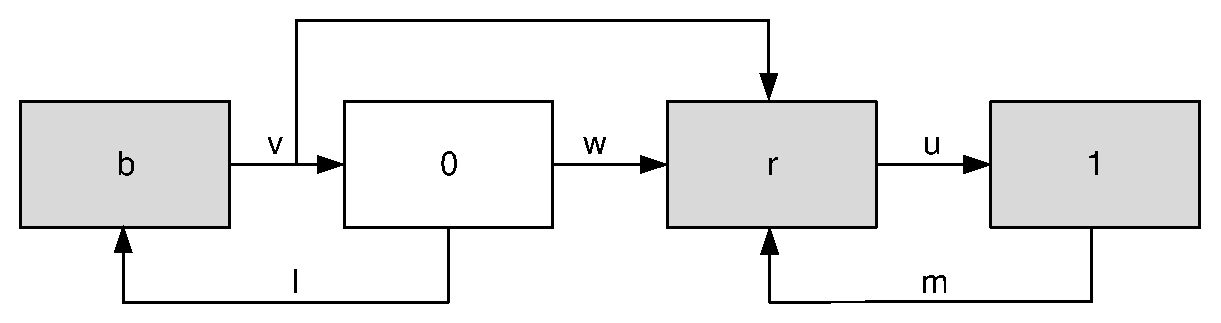
\includegraphics[width=.8\textwidth,clip, trim = 0cm 0cm 0cm 0cm]{2_KR_Trajektorienplanung_Folgeregelung.eps}
	\caption{Modellprädiktive Regelung mit nachgelagerter Folgeregelung}
	\label{fig:KR_Trajektorienplanung_Folgeregelung}
\end{figure}

Für die Implementierung der Systemerweiterung, also die weißen Kästen in Abb.\,\ref{fig:KR_Integrator_Erweiterung}-\ref{fig:KR_Trajektorienplanung_Folgeregelung}, bieten sich zwei grundsätzlich unterschiedliche Möglichkeiten an. Die erste besteht darin, die jeweiligen Differentialgleichungen mittels numerischer Standardverfahren in der Zykluszeit des Folgereglers zu lösen, also in Echtzeit zu simulieren, sodass letzterem in jedem Zeitschritt sein Referenzsignal zur Verfügung steht.
Die zweite Möglichkeit besteht darin, direkt die bei einigen Optimierungsverfahren intern als optimale Prädiktion $\bar{\bs x}^\ast(\tau)$ vorliegende Lösung heranzuziehen, s.\ Abb.\,\ref{fig:2_mpc_grundidee_u_x}. Es braucht im Anschluss des Optimierungsschritts die optimale Referenztrajektorie nur im relevanten Zeitabschnitt in der Zykluszeit des unterlagerten Reglers abgetastet und das Ergebnis zum richtigen Zeitpunkt dem Folgeregler weitergeleitet werden. Unbedingt zu beachten ist hierbei, dass nicht der Versuchung nachgegeben werden darf, anstelle von  $\tilde{\bs x}$ den gemessenen \bzw beobachteten Systemzustand $\bs x$ in die Optimierung zurückzuführen. Dann nämlich büßt das Gesamtsystem seine Robustheit gegen permanente Störungen und Modellfehler in der Weise ein, wie die fehlende Robustheit zuvor beim nicht-asymptotischen Folgeregler am Ende von Abschn.\,\ref{sec:nichtasymptotischeFolgeregelung} begründet wurde.

Zusammenfassend kann festgehalten werden, dass die Kombination aus modellprädiktivem Regelkreis und unterlagerter Folgeregelung große Vorteile in Bezug auf die Systemrobustheit bietet. 
Die Aufgabe der unterlagerten Folgeregelung ist hierbei, für ein gutmütigeres (Teil-) Streckenverhalten aus Sicht der überlagerten Optimierung zu sorgen, oder das stabilisierte System so zu beeinflussen, dass es trotz Störungen und Modellunsicherheiten dem Optimierungsmodell nahe kommt.
Hierbei entsteht aufgrund der variablen Größe des unterlagert stabilisierten Teilsystems ein Freiheitsgrad, der vom Entwicklungsingenieur so ausgenutzt werden muss, dass das Gesamtverhalten des modellprädiktiven Regelkreises ein ausgewogenes Verhältnis aus Robustheit gegen permanente Störungen bzw.\ Modellfehler und Gutmütigkeit bei Impulsstörungen aufweist. Eine generelle Empfehlung kann nicht ausgesprochen werden, da sich je nach umzusetzender Fahrerassistenzfunktion, eingesetzter Sensorik und Systemarchitektur die Anforderungen hinsichtlich Störunterdrückung, Genauigkeiten und Komfort stark unterscheiden. \\
% TODO: 
%
%Notiz: Neuplanung funkioniert bei manchen Planern nicht vom aktuellen Zustand, da dieser Stark diskretisiert ist und nur in kOmbination mit einem unterlagertn Regler funktioniert.
%
%\subsection{Praxisbeispiele}
%
% - Punktmassenmodell
% - Beispiele, die zur Motivation geführt haben, Stanford, CMU etc.
% - Exosystem
% - Führungsgröße muss für Folgeregelung hinreichend oft stetig diffbar sein (Lineare Strecke).
% - Simuliertes Modell kann vereinfacht sein (z.B. Punktmasse)
% - Sättigungsverhalten insbesondere bei Nichtlinearen Streckenteil auch interessant
%
% Werling diss: Leitet Impulsförmige Störungen auf Simuliertes System weiter, indem Zustände entsprechend gesetzt werden.
%
Zur Stabilisierung des \emph{gesamten} Fahrzustands existieren eine ganze Palette von praxiserprobten Regelungstypen, klassische \emph{PID} \cite{Muller-Bessler2006},  \emph{Sliding-mode-} \cite{eigel2010integrierte}, \citeltex{werling2014powerslide}, \emph{exakte ein-/ ausgangslinearisierende} \cite{Konig2007, atSonderheft08, soehnitz} \citeltex{werling2012trajektorienregelung}, \emph{robuste} \cite{walter_ecc2014, rathgeber_ecc2014} und \emph{optimierungsbasierte} Regler \cite{waldmann2009entwicklung, kessler2007konzept, weilkes2005zukunftige}, um nur einige zu nennen. Allesamt sind grundsätzlich dazu geeignet, auch einen reduzierten Fahrzustandsvektor zu stabilisieren. Letztendlich kann aber nur die konkrete Kombination aus MPC-Regelkreis und unterlagertem Regler auf Robustheit beurteilt werden.

%Hierbei kommen alle modernen Regelungsverfahren wie Sliding-mode \cite{eigel2010integrierte}, Exakte Ein-/Ausgangslineareisierung \cite{Konig2007, atSonderheft08} \citeltex{werling2012trajektorienregelung}, \citeltex{werling2014powerslide}
%robuste Verfahren  unterschiedliche Längs-Quer-Kopplungseffekte \cite{eigel2010integrierte} berücksichtigen. 
%\cite{waldmann2009entwicklung}  %mittels LQR-tracker

%\cite{minoiu2009driver} % Heading-control mit LMIs
%\cite{kessler2007konzept} % Lineare MPC zur Querführung für Nutzfahrzeuge -> s. auch Kap 6 Riccati
%\cite{soehnitz} % E/A-Linearisierung

% Driftregler:
% Sliding-mode: wird auch für die Querregelung eingesetzt: 
%\cite{eigel2010integrierte}
% Bestimmung des Positionsregelfehlers beim Positionstracking, zwischen den Planungszeiten.
% --macht ganzheitliche Implementierung einfacher

%\cite{Muller-Bessler2006}
%\cite{weilkes2005zukunftige} % altes Bosch paper zur Quer- und Längsführung, Kopplung in ihrem sinne

%\cite{Bender2007} 					% EP, sigmoide von proreta, keine Optimierung, parameter ergeben sich aus randbedingungen
%\cite{keller2011active} 		% EP, Polynome, keine Optimierung

 
%Zusammenfassend kann bemerkt werden, dass die großen Vorteil der ortsfesten Koordinaten für die Manöverplanung, die Positionsregelung oder das Objekt-Tracking/lokale Kartieren darin bestehen, dass die \textbf{Kopplenavigation}
%\begin{itemize}
	%\item aufgrund der Integration der Fahrzeugbewegung keinerlei Positions- und Ausrichtungssprünge aufweist (s.\ z.B.\ stanfordsmoothcoordinates),
	%\item eine nahezu permanente Verfügbarkeit aufweist und
	%\item bei Einsatz von Inertialsensorik mit einer kurze Zykluszeit (z.B.\ $\unit[10]{ms}$) verfübar ist.
%\end{itemize}
%Eine \textbf{globale Eigenlokalisierung} hingegen ist nach aktuellem Technikstand durch
%\begin{itemize}
	%\item Korrektursprünge gekennzeichnet, etwa am Tunnelende, an dem wieder ein GPS-Signal plötzlich verfügbar ist, oder bei in Sicht kommenden markanten Landmarken und
	%\item eine geringe Verfügbarkeit insbesondere innerhalb der Stadt gekennzeichnet,
%\end{itemize}
%sodass von ihr nur die Komponenten abhängen sein sollten, welche auf eine absolute Referenz angewiesen sind.
%



%Solange dessen Position, etwa von einer Kamera geliefert, in den Fahrzeugfesten Koordinaten verfügbar ist, muss sie mittels der von der Koppelnavigation gelieferten Koordinatentransformation in die Ortsfesten (wenn auch driftbehafteten) Koordinaten umgerechnet werden, wo ebenfalls das Notmanöver geplant wird. Verliert die Fahrzeugsensorik das Hindernis während des Ausweichens, so beläuft sich der Abstandsfehler zum Hindernis während des Ausweichens auf wenige Zentimeter.


%Überleitung zu smooth coordinates: trotz GPS eingesetzt weil so robust.




%Kartesische Koordinaten zu homogene Koordinaten: $[x,y]^\T \rightarrow [x,y,1]^\T$
%Translation
%\begin{align*}
	%\left[\begin{array}{c} x' \\ y' \\ 1 \end{array}\right] = \left[\begin{array}{ccc} 1 & 0 & t_x \\ 0 & 1 & t_y \\ 0 & 0 & 1 \end{array}\right] \cdot 
	%\left[\begin{array}{c} x \\ y \\ 1 \end{array}\right]
%\end{align*}
%
%Rotation
%\begin{align*}
	%\left[\begin{array}{c} x' \\ y' \\ 1 \end{array}\right] = \left[\begin{array}{ccc} \cos \alpha & -\sin\alpha & 0 \\ \sin\alpha & \cos\alpha & 0 \\ 0 & 0 & 1 \end{array}\right] \cdot 
	%\left[\begin{array}{c} x \\ y \\ 1 \end{array}\right]
%\end{align*}

% Langsame fahrt: beta_ha = 0 -> beispiel
% Triangulation
% Eine Absolute Positionierung kann sogar schädlich sein, dann wenn die Eigenlokalisierung springt, was für viele Algorithmen und Funktionen viel schlimmer ist als eine kleine durchgängige ungenauigkeit (drift)
% Erfolgt eine 1x Planung des Einparkmanövers, so muss während der Einregelung des Einparkvorgangs ebenfalls die aktuelle Position relative zur anfänglichen Position bestimmt werden, an der die Einparkkurve berechnet wurde.
% Überleitung zu Koppelnavigation: Zur Berechnung der Relativposition zu einer in der Vergangenheit liegenden Position kann die Fahrzeugbewegung aufintegriert werden und es wird von Koppelnavigation (engl. dead reckoning) gesprochen. Häufig wird Odmomentrie synonym verwendet, was aber nicht ganz korrekt ist, da streng genommen nicht nur die Räder herangezogen werden.
% Drift erklären, ist aber nicht schlimm, da nach der differenzbildung der absolutfehler sich nur auf das kleine Zeitintervall auswirkt
% Lenkradwinkel nicht vergessen bei ganz kleinen Geschwindigkeiten, da Gierratensensor dann relativ stärker driftet
% Das Ergebnis der Koppelnavigation kann zur Eigenlokalisierung verwendet werden, s. später.
% Eingangsgrößen für die Eigenlokalisierung eines Körperfesten Referenzpunkts: Bewegungsrichtung und Geschwindigkeit des Körpers im Referenzpunkt
%Zur Bestimmung der Gierbewegung eignet sich die ESP-Gierratensoensorik (hohe GEschwindigkeit) oder die Auswertung der Fahrzeugdynamik unter Berücksichtigung des aktuellen Lenkwinkels
% Insgesamt ergibt sich dann die Bewegungsdynamik zu
%\begin{align*}
	%\dot x_1 &= v \cos(\psi + \beta) \\
	%\dot x_2 &= v \sin(\psi + \beta) \\
	%\dot   \psi &= r
%\end{align*}
% Beispielbild: Drift mit großem Absolutfehler aber kleinem Relativfehler
		% Erklärung warum häufig Drift in der Loklisierung nicht schlimm ist
% Implementierung: Koppelposition wird als "korrekt" betrachtet, Ursprung kann innerhalb numerischer Genauigkeiten beliebig gewählt werden, da er sich bei der Differenzbildung aufhebt. Vorteil: Position springt nicht. Für die Verwendung absoluter Karteninformation (Straßenkarten) ist noch eine absolute Eigenlokalisierung erforderlich. Diese dient ausschließlich dazu absolute Landmarken (Straßen) in die Koppelposition zu transformieren. Zitat Stanford (smooth coordinates)
% Ich tue einfach so also ob die Koppelposition meine tatsächliche Fahrzeugposition ist und merke mir von Hindernissen etc. die Position in den lokalen Koordinaten. Habe ich das Hindernis erst kürzlich gesehen, so kann ich mir sicher sein, ...
% Wichtig auch für die Umfeldwahrnehmung und Szeneninterpretation


% ------------------------


% Falls Trajektorien für alle Zustände geplant wird, dann eignet sich Riccati zur Stabilisierung. Häufig wird aber nur für Brunowsky-Zustände geplant, dann stab durch E/A-Lin

%\label{sec:projektion} % noch unterbringen!

% Aufbau: 
% 2. Kap. Modellprädiktive Regelung im kaskadierten Regelkreis (ca. 5 Seiten) hier her kopieren, da schon sehr speziell und Kapitel sonst zu lang.
% Regelungssysteme von ABS über ESP hin zu Positionsregelung (von Stabilisierungsebene Richtung Führungsebene, Weg wird aufgezeigt, Motiviert auch, warum Hill-Climb control zb. nicht ausführlich behandelt wird, wohl aber ESP und ABS).


%\begin{figure}[h]
	%\psfrag{k}[cb][cb][1.0]{$v$}
	%\psfrag{l}[cb][cb][1.0]{$v_\text{ref}$}
	%\psfrag{m}[cb][cb][1.0]{$\lambda_1$}
	%\psfrag{n}[cb][cb][1.0]{$v_\text{Rad}$}
	%\psfrag{G}[cc][cc][1.0]{Geschwindigkeiten}
	%\psfrag{R}[cc][cc][1.0]{Radbeschleunigung}
	%\psfrag{B}[cc][cc][1.0]{Bremsdruck}
	%\psfrag{A}[cr][cr][1.0]{$A$}
	%\psfrag{b}[cr][cr][1.0]{$a$}
	%\psfrag{c}[cr][cr][1.0]{$-a$}
	%\psfrag{t}[cr][cr][1.0]{$t$}
	%\psfrag{0}[ct][ct][1.0]{Phase $0$}
	%\psfrag{1}[ct][ct][1.0]{$1$}
	%\psfrag{2}[ct][ct][1.0]{$2$}
	%\psfrag{3}[ct][ct][1.0]{$3$}
	%\psfrag{4}[ct][ct][1.0]{$4$}
	%\psfrag{5}[ct][ct][1.0]{$5$}
	%\psfrag{6}[ct][ct][1.0]{$6$}
	%\psfrag{7}[ct][ct][1.0]{$7$}
	%%\psfrag{M}[cc][cc][1.0]{Radbeschleunigung}
%\centering
%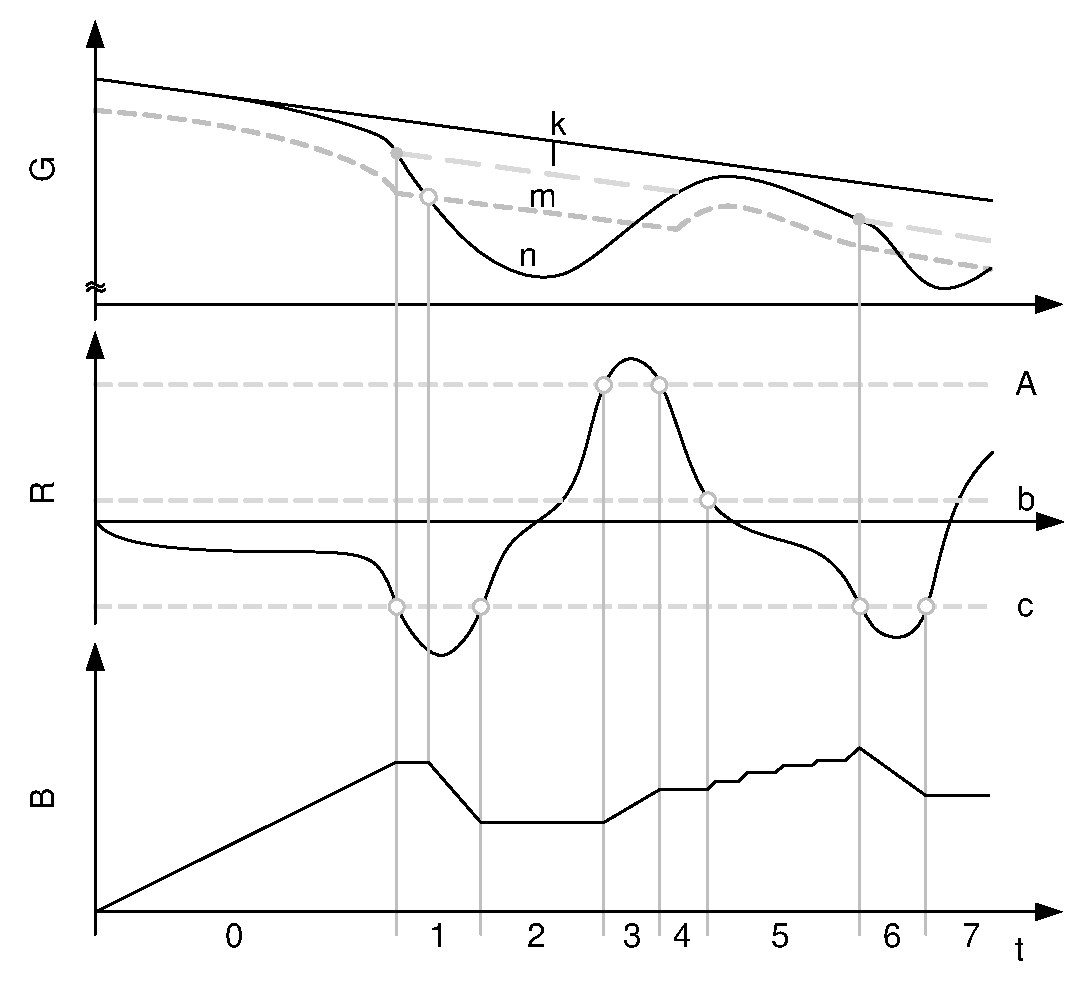
\includegraphics[width=1.0\textwidth,clip, trim = 0cm 0cm 0cm 0cm]{3_ABS_Signale.eps}
 %\caption{TODO}
 %\label{fig:abs_signale}
%\end{figure} 

% EPS Funktionen: 
% Geradeauslauf Korrektur, 
% Lane departure Warning/ support
% Fahrdynamische Lenkmomentenepfehlung (mu-split)
% Parklenkassistent


% Beispiel Seitenwindkompensation: Störbeobachter

% Überaktuiertes System -> Unterlagerte Regelung übernimmt Bremsverteilung, wird nicht in der Planung berücksichtigt
% Virtuelle Deichsel -> Heuristik
% Stanley -> Ebenfalls Heuristik -> Verallgemeinerung: E/A-Linearisierung
% ABS, ESP (Verdeutlicht am Doppelspurwechsel)

% Impedanzregelung ganz wichtig, da ja bei der Teilautomatisierung der FAhrer eine bedeutende Rolle spielt.

%[Regelung, Projektion, Invariante Fehlerdynamik]
%	\section{Systemmodellierung}
	%	\subsection{Fahrzeug} \label{sec:fahrzeugmodellierung}
	%	\subsection{Reifen} \label{sec:reifenmodellierung}
	%	\label{sec:lenkkinematik} % todo
	%	\label{sec:lenkdynamik} % todo
	%	\cite{dang2012steering} % Lenken ist viel schneller als Einzelradbremsung etc.


%\subsection{Aktorik}
%\cite{eigel2010integrierte} % Behandelt unterschiedliche Stellgrößen in der Lenkung
%\subsection{Längs- und querdynamische Kopplungseffekte}
 % und Literatur darin
% 1) Kopplung durch Geschwindigkeit (trivial)
% 2) Kopplung durch Kinematik (beim Positionstracking)
% 3) Kopplung an Reifen, dynamische Radlasten etc., Kurvenwiederstand
		
%		\subsection{Elektronisches Stabilitätsprogramm (ESP)} \label{sec:ESP}
		%\cite{BHB2012_vanZanten_bremsanlage} % Vorlage!
		%\cite{liebemann2004safety} % BOSCH ESP
		% ASR: Antrieb
		% Bremsassistent
		% Hill Hold Control
		
		% ESP muss keinen Fahrerwunsch schätzen, da durch übergeordnete Ebene Sollmanöver bekannt ist

%		\subsection{Aktiv- und Hinterachslenkung}
%		\subsection{Torque Vectoring} \label{sec:torque_vectoring}
		% \emph{torque vectoring} \cite{piyabongkarn2007use, fallah2012controller}
		% mu-split!
%[ABS, DSC]
% Seitenwindassistenz (Automatische Störgrößenkompensation, Daimler etc.)
%	\section{Fahrzeuglängsregelung}
%		\subsection{Adaptive Cruise Control (ACC)} \label{sec:acc}
%		\subsection{Notbremssysteme}
%		\label{sec:Hinterachslenkung} % todo unterbringen
%	\section{Pfadstabilisierung}
	%Fahrzeug Regelung: Literatur aus paper von Daniel Hess, IV 2013
	%\cite{atSonderheft08} %E/A-Linearisierung für Querregelung
%	\label{sec:einparksystem} %todo
% Kinematische Querregelung: ähnlichkeit mit
%\cite{Werling2010a}
%		\subsection{Projektion zur Fehlerbestimmung}
		% Abstandsbestimmung mit gradientenabstieg (s. Diss Anhang) -> Verweis auf Kap. Statische Optimierung!
%		\subsection{kinematisches Einspurmodell}
%		\section{Eingriffsstrategien}
%\begin{figure}[h]
	%\psfrag{d}[cc][c][1.0]{$\delta$}
	%\psfrag{M}[cb][cb][1.0]{$MP$}
	%\psfrag{v}[cr][cr][1.0]{$v$}
	%\psfrag{p}[cc][cc][1.0]{$\psi$}
	%\psfrag{l}[cr][cr][1.0]{$l$}
	%\psfrag{x}[cl][cl][1.0]{$[x_1, x_2]$}
%\centering
%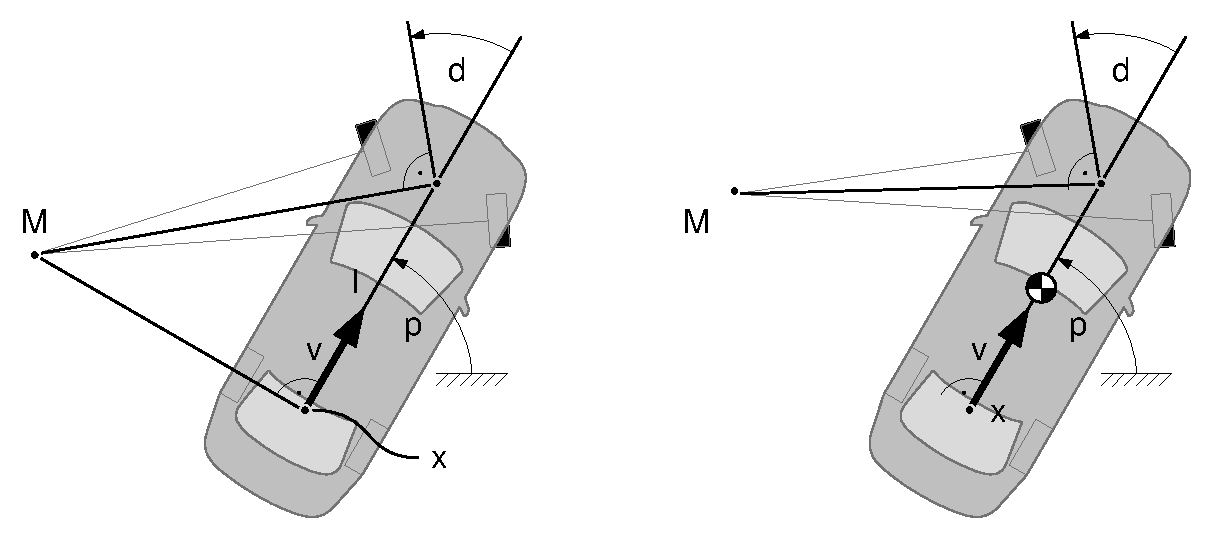
\includegraphics[width=1\textwidth,clip, trim = 0cm 0cm 0cm 0cm]{3_Einspurmodelle.eps}
 %\caption{Einspurmodell}
 %\label{fig:todo}
%\end{figure} 
		%\subsection{nichtlineares Einspurmodell}
	%\section{Trajektorienstabilisierung}
		%\subsection{Invariante Fehlerdynamik}
		%\subsection{Positionstracking}

\section{Neuer Algorithmus zur Gespannstabilisierung\index{Gespannstabilisierung}} \label{sec:anhaenger}
Während für die Vorwärtsfahrt die sog.\ \emph{aktive Gespannstabilisierung} (\emph{trailer stability assist}) \cite{BHB2012_vanZanten_bremsanlage}, \iA als Teil von ESP, das Schlingern eines Anhängers verhindert, ist der Fahrer beim rückwärtigen Rangieren auf sich alleine gestellt.
%
	%  zu erwähnen: Trailer Stability Assist (TSA)
		% Riccati zum einstellen von e/A-Z Stab Parameter
%\subsection{Hintergrund}
% Während mit dem Zugfahrzeug beim Vorwärtsfahren lediglich ein zusätzlicher Sicherheitsabstand zu kurveninneren Hindernissen eingehalten werden muss, um das Kurvenschneiden des Anhängers zu kompensieren, empfinden viele Fahrer die zum Zurücksetzen des Anhängers erforderlichen Lenkbewegungen als nicht intuitiv. 
Als nicht intuitiv wird hierbei die %nicht-holonome
Gespanndynamik empfunden, welche beim Rückwärtsfahren zur Kursänderung ein kurzzeitiges Lenken entgegen der Wunschrichtung erfordert. %Wird diese Lenktechnik nicht beherrscht, droht -- neben der Beschädigung von Fahrzeug und Anhänger -- dem Gespannführer ein nervenaufreibendes Unterfangen im öffentlichen Straßenverkehr. Hier kann eine automatische Stabilisierung des Anhängers für Entlastung des Fahrers sorgen.
Im Folgenden wird daher ein neues Stabilisierungsverfahren \citeltex{werling2014anhaenger,Werling2014trailer} für die Gierbewegung eines Anhängers vorgestellt, das den Fahrer als überlagerten Regler begreift, den es gilt, bestmöglich durch aktive Lenkeingriffe eines unterlagerten Reglers zu unterstützen. 

%Aus Kostengründen muss im Pkw-Bereich auf eine aktuierte Anhängerkupplung \cite{hoffmann2007gespannmanagement} verzichtet werden. Hierdurch steht lediglich die Lenkung zur gezielten Beeinflussung des Gespanns zur Verfügung.
Dank der interessanten nichtlinearen Struktur der Gespanndynamik existiert in der Literatur eine Vielzahl von Ansätzen, welche die Bewegung des Fahrzeuggespanns entlang vorgegebener Pfade und Trajektorien stabilisieren. Aufgrund der hohen Modellgüte sowie der einfach zu bestimmenden geometrischen Fahrzeug- und Anhängerparameter eignen sich insbesondere exakt ein-/\-ausgangs-\index{Exakte Ein-/\-ausgangslinearisierung} \bzw zustandslinearisierende\index{Zustandslinearisierung} Regelungsansätze \cite{allgower1993nichtlinearer, rothfuss1997fnz}, die auf der Kompensation der Systemnichtlinearitäten durch Zustandsrückführungen basieren. Die Herangehensweise wird auch hier verfolgt. Viele Arbeiten beschränken sich allerdings auf den Fall, bei dem der Kupplungspunkt mit dem Achsmittelpunkt des Zugfahrzeugs zusammenfällt (\emph{standard one-trailer-system}) \cite{tilbury1992steering, rouchon1993flatness2, sampei1995arbitrary}, wodurch die Mittel\-punkts\-koor\-di\-na\-ten der Anhängerachse einen flachen Ausgang (s.\ Abschn.\,\ref{sec:flachheitbasierte_para}) des Gespanns darstellen \cite{rouchon1993flatness1}. Diese Vereinfachung ist beim Pkw nicht zulässig, da der Kupplungspunktversatz %kingpin hitch, off-axle hitchching
in der Größenordnung der Länge der Anhängerdeichsel liegt \cite{altafini2001some}. \\
In \cite{rouchon1993flatness1} wird daher auch für den allgemeinen Fall (\emph{general one-trailer-system}) die Flachheit nachgewiesen. Während die Eigenschaft für eine Bahnplanung von höchstem Interesse ist (s. dazu den Ausblick in Abschn.\,\ref{sec:eval_trailer}), verzichtet der hier vorgestellte Ansatz bewusst auf die Stabilisierung eines flachen Ausgangs. Grund hierfür ist die dadurch erzielbare Reduktion der zu stabilisierenden Systemzustände, was durch die %damit verbundene 
gutmütige interne Systemdynamik des Gespanns (s.\ Abschn.\,\ref{sec:nulldynamik}) ermöglicht wird, vgl.\ \cite{Werling2010a}. \\ % Übernahme der Zeittrafo
Alternative Stabilisierungsmethoden, die den Kupplungsversatz berücksichtigen, werden in
\cite{pradalier2008robust,  % in der Praxis ist die Lenkratensättigung kein Problem, solange die Dynamik hinreichend modelliert wird, s. PT1-Modell, Kaskadiert, Kein asympt. Fehlerverhalten, schlechte Ergebnisse
schwarz2009generisches, % Kein Asymptotisches Fehlerverhalten 
gonzalez2009backing} % Kaskadiert, kein asymptotisches Tracking (s. Ergebnisse).
vorgestellt. Die dort beschriebenen Rückführungsgesetze basieren auf einer Kaskade von Querregelung und unterlagerter Knickwinkelstabilisierung. Dabei wird allerdings die Dynamik letzterer vernachlässigt, sodass die Regelung kein asymptotisches Fehlerverhalten aufweist. \\
%Der erste Teil des Beitrags greift die Idee dieser Knickwinkelstabilisierung jedoch auf, welche grundsätzlich dazu geeignet ist, dem Fahrer beim Rückwärtsfahren mit Anhänger als eigenständiges System zu assistieren. 
Die Vorteil des nachfolgend hergeleiteten Stabilisierungsgesetzes besteht darin, anstelle der Festwertregelung des Knickwinkels eine \emph{asymptotische Folgeregelung} für die \emph{Fahrkrümmung} des Anhängers zu entwerfen. Hierdurch ist es für den Fahrer möglich, etwa über einen Drehknopf, den Anhänger nahezu verzögerungsfrei zu lenken, ähnlich einem ferngesteuerten Auto. \\
%Der zweite Teil des Beitrags fokussiert auf die Pfadstabilisierung. Der hier vorgeschlagene Ansatz weist keine kaskadierte Struktur auf, sondern wird entsprechend der Vorgehensweise der exakten Ein-/Aus\-gangs\-linearisierung "`am Stück"' entworfen. Er sichert dadurch eine asymptotische Fehlerdynamik, deren Eigenwerte anhand weniger Parameter gezielt auf das Sensorrauschen abgestimmt werden können.
%im öffentlichen Straßenverkehr auch der Gesichtsverlust.

%Der Beitrag gliedert sich wie folgt. In Abschn.\,\ref{sec:anhaengerdynamik} wird zunächst das verwendete Gespannmodell vorgestellt, welches den beiden anschließenden ein-/aus\-gangs\-li\-ne\-arisier\-end\-en Reglerentwürfen zugrunde liegt.\\
%Das Modell wird in Abschn.\,\ref{sec:kruemmungsstab} einer Zeit\-trans\-for\-ma\-tion unterzogen, die der Singularitätsvermeidung im Stand dient.
%%bei den  Reglerentwürfen . 
%Der anschließende Reglerentwurf zielt auf das assistierte Zurücksetzen ab, indem der fahrergegebene Krümmungsverlauf stabilisiert wird. Wichtig hierbei ist die Vermeidung irreversibel großer Knickwinkel zwischen Fahrzeug und Anhänger sowie der Stellgrößensättigung der Lenkung. Daher wird die Nulldynamik des Systems auf Stabilität untersucht, um da\-raus Anforderungen an den Sollkrümmungsverlauf herzuleiten, welche durch die Einführung einer dynamischen Sättigungsfunktion zwischen Fahrer und Regler sicher erfüllt werden. \\
%Abschn.\,\ref{sec:pfadstab} widmet sich der Pfadstabilisierung, die zunächst eine Systemerweiterung des Gespanns um dessen zeittransformierte Pfadfolgedynamik erfordert. Im Anschluss erfolgt der zugehörige Reglerentwurf, wobei auf Ergebnisse des vorangegangen Abschnitts zurückgegriffen wird. \\
%Die Evaluation der vorgestellten Regelungskonzepte erfolgt schließlich in Abschn.\,\ref{sec:eval_trailer} anhand realer Fahrversuche mit einem Pkw-Gespann. 


\subsection{Nichtlineare Anhängerdynamik} \label{sec:anhaengerdynamik}
Da Anhänger grundsätzlich nur mit niedrigen Querbeschleunigungen zurückgesetzt werden, können die sog.\ Schräglaufwinkel an den Reifen des Gespanns vernachlässigt werden. Wie Abb.\,\ref{fig:KESM_Gespann} verdeutlicht, definieren hierdurch die Reifenausrichtungen über die Momentanpole $\mathrm{MP}_v$ und $\mathrm{MP}_t$ die Kinematik von Fahrzeug und Anhänger. Mit der Fahrzeugausrichtung $\psi_v$ und der Hinterachsgeschwindigkeit $v_v<0$ sowie mit dem effektiven Lenkwinkel $\delta$ der Vorderräder und dem Achsabstand $l_v>0$ ergibt sich die Fahrzeuggierdynamik (vgl.\ \zB \cite{atSonderheft08}) zu
%$l_v$ Hypotenuse
\begin{align}
	\dot \psi_v & = v_v \frac{\tan\delta}{l_v} \label{eq:fzgmodell:psi_v_dot}.
\end{align}
Entsprechend der Herleitung in \ref{app:herleitung_anhaengerdynamik} wird die Anhängergierdynamik durch
\begin{align}
\negspace	 
	\dot\psi_t &= \frac{v_v}{l_t} \left[\sin\left(\psi_v \! - \! \psi_t\right) - l_c\cos\left(\psi_v  \! - \!\psi_t\right) \frac{\tan\delta}{l_v} \right]  \label{eq:fzgmodell:psi_t_dot}
\end{align}
mit der vorzeichenbehafteten Anhängergeschwindigkeit 
\begin{align}
\negspace
	v_t &:= v_v \left[ \cos\left(\psi_v  \! - \! \psi_t\right) + l_c\sin\left(\psi_v  \! - \! \psi_t\right) \frac{\tan\delta}{l_v} \right] \label{eq:fzgmodell:v_t}
\end{align}
beschrieben. %An dieser Stelle sei angemerkt, dass die Betrachtung der Fahrzeuggeschwindigkeit $v_v<0$ als zeitabhängiger Systemparameter sowohl die Kombination mit einer manuellen (s.\ später Abschn.\,\ref{sec:eval_trailer}) als auch mit einer separaten automatischen Antriebsregelung ermöglicht. Dadurch ist die Lenkung als alleiniger Systemeingang anzusehen. 
Zur Vermeidung von Überschwingen ist das Verzögerungsverhalten der Lenkaktorik unbedingt zu modellieren und im Entwurf zu berücksichtigen. In der Praxis hat sich aufgrund der schnellen Dynamik der unterlagert eingesetzten Moment- und Drehratenregelung die Modellierung des Lenkwinkelübertragungsverhaltens %r Winkelpositionsregelung 
der Aktorik als PT$_1$-Glied
\begin{align}
	\dot\delta &= \frac{1}{T}\left[u-\delta\right] \label{eq:assistiert:delta_dot}
\end{align}
bewährt \cite{pradalier2008robust}. Hierbei beschreibt $T>0$ die Zeitkonstante und $u$ die dem Lenkaktor übermittelte Sollvorgabe -- und damit die Stellgröße des Systems. % hab: Kleinsignalverhalten!

\begin{figure}
    \psfrag{MPv}[lb][lb][1.0]{$\mathrm{MP}_v$}
	\psfrag{MPt}[lc][lc][1.0]{$\mathrm{MP}_t$}
	\psfrag{delta}[cc][cc][1.0]{$\delta$}
	\psfrag{rv}[lt][lt][1.0]{$\boldsymbol r_v$}
	\psfrag{rt}[rb][rb][1.0]{$\boldsymbol r_t$}
	\psfrag{rc}[cc][cc][1.0]{$\boldsymbol r_c$}
	\psfrag{vv}[rb][rb][1.0]{$\boldsymbol v_v$}
	\psfrag{vt}[lt][tl][1.0]{$\,\boldsymbol v_t$}
	\psfrag{vh}[lc][lc][1.0]{$\boldsymbol v_c$}
	\psfrag{psiv}[tr][tr][1.0]{$\psi_v$}
	\psfrag{psit}[rt][rt][1.0]{$\psi_t$}
	\psfrag{dpsi}[lb][lb][1.0]{$\,\Delta\psi$}
	\psfrag{lt}[rb][rb][1.0]{$l_t$}	
	\psfrag{lv}[rb][rb][1.0]{$l_v$}	
	\psfrag{lc}[rb][rb][1.0]{$l_c$}	
    \centering
    \includegraphics[width=.6 \linewidth,trim = 0cm 0cm 0cm 0cm]{3_KESM_Gespann.eps}
    \caption[Kinematisches Einspurmodell des Fahrzeuggespanns]{Kinematisches Einspurmodell des Fahrzeuggespanns \citeltex{werling2014anhaenger}}
    \label{fig:KESM_Gespann}
\end{figure}



%\subsection{Gierdynamikstabilisierung des Anhängers} \label{sec:kruemmungsstab}
\subsection{Zeittransformation} \label{sec:zeittrafo}
%Da im Stand zur Stabilisierung mittels glatter Rückführung das notwendige Brockett-Theorem \cite{brockett1983asa} verletzt ist.
Aufgrund der Nicht-Holonomie des Systems wird mit abnehmender Absolutgeschwindigkeit eine asymptotische Stabilisierung des Anhängers mittels stetiger Rückführung zunehmend schwieriger \cite{brockett1983asa}. Aus dem Grund wird auf eine Stabilisierung im Stand zugunsten eines ruhigen Anhaltevorgangs bewusst verzichtet. Das erfolgt implizit, indem die Gespanndynamik anstelle der Zeit $t$ für eine neue unabhängige Variable $s_t$ mit $\dot s_t(t)\geq 0$ formuliert wird \cite{sampei1988robot,sampei1986tsn}, für die eine asymptotische Stabilisierung umgesetzt werden kann. Da die neue Zeit immer dann stehen bleiben muss, wenn es das Gespann tut, eignet sich prinzipiell die \emph{zurückgelegte Wegstrecke} eines jeden Punkts von Fahrzeug und Anhänger dafür. Die Formeln vereinfachen sich jedoch stark, wenn der Hinterachsmittelpunkt des Anhängers herangezogen wird, sodass
\begin{align*}
	s_t(t):=\int_0^t |v_t(\tau)| \, {\rm d} \tau
\end{align*}
gewählt wird und damit die Transformationsvorschrift
\begin{equation}
	\dot{()} := \diff{}{t} =  \diff{}{s_t} \diff{s_t}{t} = ()' \cdot (-v_t) \label{equ:timetrafo}
\end{equation}
für $v_t<0$ gilt. Mit dem Knickwinkel\index{Knickwinkel} $\Delta \psi := \psi_v - \psi_t$, s. Abb.\,\ref{fig:KESM_Gespann},
wird hierdurch für $\bldx = [\Delta \psi, \delta]^\T$ das zeittransformierte, eingangsaffine System
\begin{subequations} \label{equ:zeittransformiertes_system}
\begin{align}
\label{equ:zeittransformiertes_system_dynamics}
	\boldsymbol x^\prime &= \boldsymbol f(\boldsymbol x) + \boldsymbol g(\boldsymbol x) u, \quad \boldsymbol x(0) = \boldsymbol x_0\\
	y &= h(\boldsymbol x) \label{equ:zeittransformiertes_system_output}
\end{align}
mit
\end{subequations}
\begin{subequations}
\begin{align*}
\negspace\negspace
	\boldsymbol f(\boldsymbol x) &= \begin{bmatrix} \dfrac{-l_t\tan \delta+l_v\sin \Delta \psi-l_c\cos \Delta \psi\tan \delta}{l_t\left[l_v\cos \Delta \psi+l_c\sin \Delta \psi\tan \delta\right]} \\ \dfrac{l_v\delta}{T v_v\left[l_v\cos \Delta \psi+l_c\sin \Delta \psi\tan \delta\right]} \end{bmatrix}\\
\negspace\negspace
	\boldsymbol g(\boldsymbol x) &= \begin{bmatrix} 0 \\ -\dfrac{l_v}{T v_v\left[l_v\cos \Delta \psi+l_c\sin \Delta \psi\tan \delta\right]}\end{bmatrix}
\end{align*}
\end{subequations}
erhalten \citeltex{werling2014anhaenger}. Die Ausgangsabbildung $h(\boldsymbol x)$ stellt 
die Kurskrümmung des Anhängers dar.
Da hier der in der Literatur verbreiteten Vorzeichenkonvention gefolgt wird, ist die Anhängerkurskrümmung definitionsgemäß die Orientierungsänderung pro \emph{vorwärts} zurückgelegter Wegstrecke, also $\kappa_t = -\psi_t'$\,, und damit
\begin{align}
	h(\boldsymbol x) = \frac{l_v\sin\Delta\psi-l_c\cos\Delta\psi\tan\delta}{l_t\left[l_v\cos\Delta\psi+l_c\sin\Delta\psi\tan\delta\right]}\;.\label{eq:assistiert:kruemmung}
\end{align}
Es gilt nun, den Ausgang entsprechend der Sollkurskrümmung $y_d= \kappa_{t,d}(s_t)$ in Abhängigkeit von der zurückgelegten Wegstrecke $s_t$ asymptotisch zu stabilisieren.



\subsection{Nichtlinearer Reglerentwurf}  \label{sec:kruemmungsstab_entwurf}
Entsprechend der Vorgehensweise der Ein-/Aus\-gangs\-linearisierung (s.\ \zB \cite{allgower1993nichtlinearer, rothfuss1997fnz, isidori1995ncs, kok95}) wird nun der Ausgang so oft abgeleitet -- infolge der Zeittransformation \eqref{equ:timetrafo} nach der vom Anhänger zurückgelegten Wegstrecke $s_t$ -- bis der Eingang $u$ erscheint. Aufgrund des relativen Grads von Eins erfolgt dies bereits im ersten Schritt. Mit der abkürzenden Darstellung mittels Lie-Ableitung wird hierbei
\begin{align}
\nonumber
	h'(\bldx) &= \Lie_f h(\bldx) + \underbrace{\Lie_gh(\boldsymbol x)}_{\neq 0} u %- \kappa'_{t,d}
	= \\[1ex]
\nonumber
	& \frac{\left[l_v^2\!+\!l_c^2\tan^2 \delta\right]\left[-l_t\tan \delta+l_v \sin \Delta \psi-l_c \cos \Delta \psi\tan \delta\right]}{l_t^2\left[l_v\cos \Delta \psi+l_c\sin \Delta \psi\tan \delta\right]^3}\\
\nonumber
	& -\frac{l_v^2l_c\delta}{l_tTv_v\cos^2\!\delta \left[l_v\cos \Delta \psi+l_c\sin \Delta \psi\tan \delta\right]^3} \\
	%\end{split}
 & + \frac{l_v^2l_c}{l_tTv_v\cos^2\!\delta \left[l_v\cos \Delta \psi+l_c\sin \Delta \psi\tan \delta\right]^3} u % - \kappa'_{t,d} \\
 \label{equ:ersteAbleitung_kruemmung}
%	\end{split}
\end{align}
erhalten. Für die linearisierende Rückführung
% E/A-Linearisierung
\begin{align}
\nonumber
%\negspace\negspace
	u &= \frac{1}{\Lie_g h(\boldsymbol x)} \left[\kappa'_{t,d}(s_t) -\Lie_fh(\boldsymbol x) +\nu\right] = \\[2ex] \nonumber
\negspace\negspace		
		&\frac{l_tTv_v\cos^2\!\delta}{l_v^2 l_c}\Biggl[\!\left[l_v\cos \Delta \psi+l_c\sin \Delta \psi\tan \delta\right]^3 [\kappa'_{t,d}(s_t)\!+\!\nu] 	\\[2ex]
%\negspace\negspace
		& - \!\frac{\!\left[l_v^2\!+\!l_c^2\tan^2 \delta\right]\!\!\left[-l_t\!\tan \delta+l_v\! \sin \Delta \psi-l_c \!\cos \Delta \psi\tan \delta\right]\!}{l_t^2}\Biggr]
 + \delta \;, \label{equ:linearisierendeRueckfuehrungKruemmung}
\end{align}
mit $l_v,l_c,l_t > 0$ und $|\delta| < \nicefrac{\pi}{2}$
ergibt sich in den Fehlerkoordinaten % der Koordinatentransformation 
\begin{align}
	\xi = h(\bldx) - \kappa_{t,d}(s_t) \label{equ:trafo_kruemmung}
\end{align}
das Integratorsystem
\begin{equation} \label{equ:integratorsystem_kruemmung}
	\xi' = \nu; \quad \xi(0) = 0
\end{equation}
mit neuem Eingang $\nu$.
Die Stabilisierung erfolgt standardmäßig durch %die Rückführung 
\begin{equation}
	\nu = -k \xi ; \quad k > 0 \;.% = -k [\kappa_t - \kappa_{t,d}] \quad \text{mit} \quad k > 0.  
	\label{equ:zustandsregler_kruemmung}
\end{equation}
%des transformierten Zustands.

Durch den relativen Grad von Eins verbleibt für das System zweiter Ordnung eine \sog interne Dynamik \cite{svaricek2006nln}, die sich in der Koordinate $\eta = \Delta\psi$ als
\begin{equation}
	\eta' = -\frac{1}{l_c}\sin\eta + \left[1+\dfrac{l_t}{l_c}\cos\eta\right] [\kappa_{t,d}+\xi]; \quad \eta(0) = \psi_0 \label{equ:internedynamik_kruemmung}
\end{equation}
%mit Anfangszustand $\eta_0$ 
darstellt. 
%Da sich der Fahrer darauf verlassen können muss, dass der Anhänger nicht so stark einknickt, dass er die maximale invariante Menge verlässt und demnach mit dem verfügbaren Lenkwinkel nicht mehr stabilisiert werden kann, muss die Krümmungssollvorgabe des Fahrers, welche das Sys\-tem \eqref{equ:internedynamik_kruemmung} als $\kappa_{t,d}$ anregt, überwacht und \ggf korrigiert werden. Dies erfolgt im nächsten Abschnitt.
%Da der Knickwinkel $\Delta\psi$ konstruktiv beschränkt ist, wird \eqref{equ:internedynamik_kruemmung} im nachfolgenden Kapitel einer ausgiebigen Analyse unterzogen.

\subsection{Nulldynamik\index{Nulldynamik} und Sollwertvorgaben} \label{sec:nulldynamik}
Vereinfachend wird angenommen, dass der Regelfehler bereits abgeklungen ist, d.h.\ $y\equiv y_d$ und damit $\xi \equiv 0$. Hierdurch stellt sich \eqref{equ:internedynamik_kruemmung} dar als
\begin{equation}
	\Delta\psi^\prime(\Delta\psi, \kappa_{t,d}) = -\frac{1}{l_c}\sin\Delta\psi + \left[1+\dfrac{l_t}{l_c}\cos\Delta\psi\right]\kappa_{t,d}, \label{equ:zerodynamics}
\end{equation}
was als \sog Nulldynamik bezeichnet wird \cite{svaricek2006nln}. Die Annahme $\xi \equiv 0$ ist in der Praxis gerechtfertigt, wenn zusätzlich zur asymptotischen Fehlerdynamik sichergestellt wird, dass nicht nur die Sollvorgabe hinreichend oft stetig differenzierbar ist, sondern bei Aktivierung des Systems mit dem Istwert abgeglichen wird, was durch die Anfangsbedingungen in \eqref{equ:integratorsystem_kruemmung} bereits gegeben ist (s.\ auch später Abschn.\,\ref{sec:eval_trailer}). \\
Ziel ist es nun, unter Berücksichtigung der Nulldynamik
%von \eqref{eq:assistiert:kruemmung} und \eqref{equ:zerodynamics} 
Anforderungen an die Sollvorgabe $\kappa_{t,d}$ abzuleiten, welche das Sys\-tem \eqref{equ:internedynamik_kruemmung} als $\kappa_{t,d}$ anregt, sodass automatisch dafür gesorgt wird, dass weder der Knickwinkel seinen zulässigen Bereich verlässt, noch der verfügbare Lenkwinkel überschritten wird. Entsprechend Abschn.\,\ref{sec:invariantSets} darf also die maximale control-invariante Menge der Strecke nicht verlassen werden.

\subsubsection{Instantan stabilisierbare Maximalkrümmung}
Um sicherzustellen, dass der verfügbare Lenkwinkel \emph{instantan} ausreicht, die Sollkrümmung zu \emph{stabilisieren}, wird der tatsächlich verfügbare Lenkwinkel\footnote{Die Berücksichtigung ungleicher Maximal- und Minimallenkwinkel erfolgt analog.} um eine kleine Regelreserve reduziert und im Folgenden als $\delta_\text{max}$ bezeichnet. \\
Für die Nulldynamik gilt $y \equiv y_d$, also $\kappa_{t}(\Delta\psi, \delta) \equiv \kappa_{t,d}$, sodass sich die Reglersollvorgabe direkt auf den Lenkwinkel auswirkt.
Aufgrund der strengen Monotonie von \eqref{eq:assistiert:kruemmung} im relevanten Bereich bzgl.\ des Lenkwinkels ($\tfrac{\partial \kappa_t}{\partial\delta}<0$) ist in der Gleichung die Variable $\delta$ durch den verfügbaren Maximallenkwinkel $\delta_\text{max}$ zu ersetzen, d.h.\
\begin{align*}
	\kappa_t(\Delta\psi, \delta_\text{max})=:\kappa_{t,\text{max,inst}}(\Delta\psi),
\end{align*}
 und es reicht aus, zur Vermeidung von Lenkanschlägen
\begin{align} \label{equ:kappa_max_inst}
	|\kappa_{t,d}| < \kappa_{t,\text{max,inst}}(\Delta\psi)
\end{align}
in jedem Zeitschritt sicherzustellen. Folglich ist die instantan umsetzbare Sollkrümmung abhängig vom aktuellen Knickwinkel $\Delta\psi$ und ändert sich damit permanent im instationären Fall.

\subsubsection{Stationär stabilisierbare Maximalkrümmung}
Aus der Fahrpraxis ist bekannt, dass ein zu stark abgewinkelter Anhänger auch durch sofortiges Gegenlenken mit Maximaleinschlag nicht am weiteren Einknicken gehindert werden kann, also seine control-invariante Menge verlassen hat. Da \eqref{equ:kappa_max_inst} lediglich eine für die Stabilisierung erforderliche marginale Lenkreserve instantan sicherstellt, muss zusätzlich gefordert werden, dass $\kappa_{t,d}$ keinen \emph{irreversibel} großen Knickwinkel $\Delta\psi$ provoziert. Gesucht wird also eine obere Schranke $|\kappa_{t,d}|<\kappa_{t,\text{max},\text{stat}}=\text{const.}$\footnote{Es kann auch eine dynamische obere Schranke in Abhängigkeit des aktuellen Knickwinkels gefunden werden, die weniger konservativ, jedoch aufwändiger zu berücksichtigen ist.}, sodass der Knickwinkel innerhalb eines zulässigen Bereichs $|\Delta\psi| < \Delta\psi_\text{max}$ bleibt. Aus Gründen der Symmetrie reicht es aus, den Fall $ \Delta\psi > 0$ zu betrachten.

Um die Beschränktheit des Knickwinkels sicherzustellen, ist $\Delta\psi'(\Delta\psi=\Delta\psi_\text{max}) < 0$ zu fordern. Aufgrund der Monotonie von \eqref{equ:zerodynamics} ($\tfrac{\partial \Delta\psi'}{\partial \kappa_{t,d}}<0$) gilt
\begin{align*}
	\Delta\psi'(\Delta\psi_\text{max}, \kappa_{t,d}) < \Delta\psi'(\Delta\psi_{\text{max}}, \kappa_{t,\text{max},\text{stat}}) = 0.
\end{align*}
Durch Auflösen von \eqref{equ:zerodynamics} ergibt sich damit
\begin{align}
	\kappa_{t,\text{max}, \text{stat}} = \frac{\sin \Delta\psi_\text{max}}{l_c + l_t \cos \Delta\psi_\text{max}} \;. \label{eq:kappatdmax}
\end{align}

\begin{figure}[ht]
	%\centering
	% Erste Figure	
	\def\xlabel{$\Delta\psi$ in \unit{rad}}
	\def\ylabel{$\,\,\,\,\,\,\,\,\,\,\,\,\,\,\,\Delta\psi'(\pm\delta_{\text{max},\text{stat}})$ in \unitfrac{rad}{s}}		
	% Generated using matlabfrag
% Version: v0.6.16
% Version Date: 04-Apr-2010
% Author: Zebb Prime
%
%% <text>
%
\providecommand\matlabtextA{\color[rgb]{0.000,0.000,0.000}\fontsize{10}{10}\selectfont\strut}%
\psfrag{012}[tc][tc]{\matlabtextA \ylabel}%
\psfrag{013}[bc][bc]{\matlabtextA \xlabel}%
%
%% </text>
%
%% <xtick>
%
\def\matlabfragNegXTick{\mathord{\makebox[0pt][r]{$-$}}}
%
\providecommand\matlabtextB{\color[rgb]{0.000,0.000,0.000}\fontsize{11}{11}\selectfont\strut}%
\psfrag{000}[ct][ct]{\matlabtextB $-\pi$}%
\psfrag{001}[ct][ct]{\matlabtextB $-\frac{\pi}{2}$}%
\psfrag{002}[ct][ct]{\matlabtextB $-\psi_{\text{max},\text{stat}}$}%
\psfrag{003}[ct][ct]{\matlabtextB 0}%
\psfrag{004}[ct][ct]{\matlabtextB $\psi_{\text{max},\text{stat}}$}%
\psfrag{005}[ct][ct]{\matlabtextB $\frac{\pi}{2}$}%
\psfrag{006}[ct][ct]{\matlabtextB $\pi$}%
%
%% </xtick>
%
%% <ytick>
%
\psfrag{007}[rc][rc]{\matlabtextB $-0.8$}%
\psfrag{008}[rc][rc]{\matlabtextB $-0.4$}%
\psfrag{009}[rc][rc]{\matlabtextB $0$}%
\psfrag{010}[rc][rc]{\matlabtextB $0.4$}%
\psfrag{011}[rc][rc]{\matlabtextB $0.8$}%
%
%% </ytick>
	\renewcommand{\matlabtextA}{\scriptsize}
	\renewcommand{\matlabtextB}{\scriptsize}
    \subfigure[kurzer Anhänger ($l_t < l_{t,\text{lim}}$)]{
		\includegraphics[width=.5 \linewidth,trim = 0cm 0cm 0cm 0cm]{3_Maximaler_Knickwinkel_Laenge1_Paper.eps}\label{fig:Maximaler_Knickwinkel_Vergleich_kurz}} %\\[3ex]
	% Zweite Figure	
	% Generated using matlabfrag
% Version: v0.6.16
% Version Date: 04-Apr-2010
% Author: Zebb Prime
%
%% <text>
%
\providecommand\matlabtextA{\color[rgb]{0.000,0.000,0.000}\fontsize{10}{10}\selectfont\strut}%
\psfrag{010}[tc][tc]{\matlabtextA \ylabel}%
\psfrag{011}[bc][bc]{\matlabtextA \xlabel}%
%
%% </text>
%
%% <xtick>
%
\def\matlabfragNegXTick{\mathord{\makebox[0pt][r]{$-$}}}
%
\providecommand\matlabtextB{\color[rgb]{0.000,0.000,0.000}\fontsize{11}{11}\selectfont\strut}%
\psfrag{000}[ct][ct]{\matlabtextB $-\pi$}%
\psfrag{001}[ct][ct]{\matlabtextB $-\frac{\pi}{2}$}%
\psfrag{002}[ct][ct]{\matlabtextB 0}%
\psfrag{003}[ct][ct]{\matlabtextB $\frac{\pi}{2}$}%
\psfrag{004}[ct][ct]{\matlabtextB $\pi$}%
%
%% </xtick>
%
%% <ytick>
%
\psfrag{005}[rc][rc]{\matlabtextB $-0.8$}%
\psfrag{006}[rc][rc]{\matlabtextB $-0.4$}%
\psfrag{007}[rc][rc]{\matlabtextB $0$}%
\psfrag{008}[rc][rc]{\matlabtextB $0.4$}%
\psfrag{009}[rc][rc]{\matlabtextB $0.8$}%
%
%% </ytick>
    \subfigure[langer Anhänger ($l_t > l_{t,\text{lim}}$)]{
		\includegraphics[width=.5 \linewidth,trim = 0cm 0cm 0cm 0cm]{3_Maximaler_Knickwinkel_Laenge2_Paper.eps}\label{fig:Maximaler_Knickwinkel_Vergleich_lang}}
	% Beschriftung
    \caption[Realisierbare Knickwinkeländerungsraten]{Durch maximalen und minimalen Lenkeinschlag  (obere und untere schwarze Linie) gegebener Bereich (grau) der Knickwinkeländerungsrate in Abhängigkeit des Knickwinkels \citeltex{werling2014anhaenger}}
    \label{fig:Maximaler_Knickwinkel_Vergleich}
\end{figure}


Zur Festlegung von $\Delta\psi_\text{max}$ wiederum muss der für die Fahrzeug- und Anhängergeometrie zulässige Maximalknickwinkel $\Delta\psi_\text{max,geom}$ aus den Gespannparametern bestimmt werden. Er ist mit dem durch den zulässigen Lenkwinkel $\delta_{\text{max},\text{stat}}$ stationär stabilisierbaren Knickwinkel $\Delta\psi_\text{max,stat}$ mittels
\begin{align}
	\Delta\psi_\text{max} = \text{min}(\Delta\psi_\text{max,geom}, \Delta\psi_\text{max,stat})
\end{align}
 zu vergleichen. Letzterer wird für Anhänger mit $l_t \leq l_{\rm t,lim}$,
\begin{equation*}
	l_{\rm t,lim} = \sqrt{\frac{l_v^2}{\tan^2\delta_{\text{max},\text{stat}}}+l_c^2}, %\label{eq:assistiert:ltlim}
\end{equation*}
erhalten (vgl.\ Abb.\,\ref{fig:Maximaler_Knickwinkel_Vergleich_kurz}), indem wieder
die Nulldynamik mit $\kappa_{t,d} \equiv \kappa_{t}$ herangezogen wird. Gleichsetzen von \eqref{eq:assistiert:kruemmung} zum maximal zulässigen Lenkwinkel $\delta_{\text{max},\text{stat}}$ und  \eqref{eq:kappatdmax} liefert nach einigen Umformungen den maximal zulässigen Knickwinkel
\begin{equation}
	\Delta\psi_{\text{max},\text{stat}} = \arccos\left( -c_1 + \sqrt{c_2 + c_1^2} \right) \label{equ:eta_max_stat}
\end{equation}
mit
\begin{equation*}
	c_1 = \frac{l_c l_t \tan^2\delta_{\text{max},\text{stat}}}{l_v^2 + l_c^2 \tan^2\delta_{\text{max},\text{stat}}}, \quad
	c_2 = \frac{l_v^2 - l_t^2 \tan^2\delta_{\text{max},\text{stat}}}{l_v^2 + l_c^2 \tan^2\delta_{\text{max},\text{stat}}}.
\end{equation*}


\begin{figure}[ht]
	\centering
	% Erste Figure	
	\def\xlabel{$l_t$ in \unit{m}}
	\def\ylabel{$\Delta\psi_\text{max,geom}, \Delta\psi_\text{max,stat}$ in \unit{rad}}	
	% Generated using matlabfrag
% Version: v0.6.16
% Version Date: 04-Apr-2010
% Author: Zebb Prime
%
%% <text>
%
\providecommand\matlabtextA{\color[rgb]{0.000,0.000,0.000}\fontsize{10}{10}\selectfont\strut}%
\psfrag{013}[cc][cc]{\matlabtextA zulässiger Knickwinkel}%
%
\providecommand\matlabtextB{\color[rgb]{0.000,0.000,0.000}\fontsize{11}{11}\selectfont\strut}%
\psfrag{011}[bc][bc]{\matlabtextB \xlabel}%
\psfrag{012}[tc][tc]{\matlabtextB \ylabel}%
%
%% </text>
%
%% <xtick>
%
\def\matlabfragNegXTick{\mathord{\makebox[0pt][r]{$-$}}}
%
\psfrag{000}[ct][ct]{\matlabtextB 0}%
\psfrag{001}[ct][ct]{\matlabtextB 1}%
\psfrag{002}[ct][ct]{\matlabtextB 2}%
\psfrag{003}[ct][ct]{\matlabtextB 3}%
\psfrag{004}[ct][ct]{\matlabtextB 4}%
\psfrag{005}[ct][ct]{\matlabtextB $l_{t,\text{lim}}$}%
\psfrag{006}[ct][ct]{\matlabtextB 5}%
%
%% </xtick>
%
%% <ytick>
%
\psfrag{007}[rc][rc]{\matlabtextB 0}%
\psfrag{008}[rc][rc]{\matlabtextB $\frac{\pi}{4}$}%
\psfrag{009}[rc][rc]{\matlabtextB $\frac{\pi}{2}$}%
\psfrag{010}[rc][rc]{\matlabtextB $\frac{3\pi}{4}$}%
%
%% </ytick>
	%\renewcommand{\matlabtextA}{\footnotesize}
	%\renewcommand{\matlabtextB}{\scriptsize}
	\renewcommand{\matlabtextB}{\small}
	\includegraphics[width=.7 \linewidth,trim = 0cm 0cm 0cm 0cm]{3_Maximaler_Knickwinkel_Paper.eps}
	% Beschriftung
    \caption[Zulässiger Absolutknickwinkel]{Zulässiger Absolutknickwinkel $\Delta\psi_\text{max,stat}$ (schwarz) in Abhängigkeit der Anhängerlänge sowie konstruktiver Grenzwert $\Delta\psi_\text{max,geom}$ (gestrichelt) für typische Fahrzeugparameter \citeltex{werling2014anhaenger}}
    \label{fig:Maximaler_Knickwinkel}
\end{figure}


Da eine Krümmungsänderung des Anhängers immer mit einer gegensinnigen Lenkbewegung eingeleitet wird, muss $\delta_{\text{max},\text{stat}}$ merklich kleiner gewählt werden als $\delta_{\text{max}}$. Ansonsten dauert der Übergang aufgrund des dynamischen Sättigungsverhaltens zu lange. \\ %(s.\ später Abschn.\,\ref{sec:eval_kruemmungsstab}). \\
Für Anhänger mit $l_t > l_{\rm t,lim}$ hingegen existiert keine reelle Lösung von \eqref{equ:eta_max_stat}, was sich praktisch darin äußert, dass $\delta_{\text{max},\text{stat}}$ grundsätzlich ausreicht, den Anhänger zu stabilisieren (s.\ Abb.\,\ref{fig:Maximaler_Knickwinkel_Vergleich_lang}), sodass der konstruktive Grenzwert $\Delta\psi_\text{max,geom}$ (s.\ gestrichelte Linie in Abb.\,\ref{fig:Maximaler_Knickwinkel}) den maximalen Knickwinkel beschränkt.

%Bei Fahrt mit stationärem Knickwinkel fallen in Abb.\,\ref{fig:KESM_Gespann} $\mathrm{MP}_t$ und $\mathrm{MP}_v$ zu einem gemeinsamen Momentanpol $\mathrm{MP}$ zusammen. Wird nun in diesem stationären Fall die Anhängerdeichsellänge $l_t$ gedanklich verlängert, so wandert der Anhängerachsmittelpunkt in Richtung $\mathrm{MP}$, bis auch diese beiden Punkte zusammenfallen und sich das Fahrzeug um den stationären Anhängerachsmittelpunkt dreht.

%Geometrischer Maximalknickwinkel $\Delta\psi_\text{max,geom}$ und stationär stabilisierbarer Maximalknickwinkel $\Delta\psi_\text{max,stat}$
%\begin{align}
	%\Delta\psi_\text{max} = \text{min}(\Delta\psi_\text{max,stat}, \Delta\psi_\text{max,geom})
%\end{align}
%Mit $\Delta\psi' = 0$ und $\Delta\psi = \Delta\psi_\text{max}$ liefert die erste Zeile von \eqref{equ:zeittransformiertes_system_dynamics} nach Auflösen und
%einsetzen in 
%\eqref{eq:assistiert:kruemmung}
%\begin{align}
	%\kappa_{t,\text{max,stat}} = \kappa(\Delta\psi_\text{max},\delta(\Delta\psi_\text{max})).
%\end{align}

\subsubsection{Automatische Korrektur der manuellen Krümmungsvorgaben}
Zur Vermeidung der mit zu hohen Sollkrümmungsvorgaben $\kappa_\text{man}$ des Fahrers verbundenen Instabilität muss jetzt lediglich sichergestellt werden, dass diese zu jedem Zeitpunkt die zuvor hergeleiteten hinreichenden Bedingungen \eqref{equ:kappa_max_inst} und \eqref{eq:kappatdmax}   einhalten. Eine gleichermaßen einfache wie für den Fahrer intuitive Möglichkeit ist hierfür die Zwischenschaltung eines statischen und  dynamischen Sättigungsglieds, und zwar
\newcommand{\sat}[2]{\text{sat}_{#1}^{#2}}
\begin{align}
	 \negspace \kappa_{t,d} = \sat{-\kappa_{t,\text{max,inst}(\Delta\psi)}}{\kappa_{t,\text{max,inst}(\Delta\psi)}} \left(\, \sat{-\kappa_{t,\text{max,stat}}}{\kappa_{t,\text{max,stat}}}(\kappa_\text{man})\,\right).
\end{align}

Eine Übersichtsdarstellung der Reglerstruktur kann Abb.\,\ref{fig:KrAblauf} entnommen werden.

\begin{figure}[ht]
	\centering
   \psfrag{boxeins}[cc][cc][0.8]{\eqref{eq:fzgmodell:psi_v_dot}\,-\,\eqref{eq:assistiert:delta_dot}}
	\psfrag{boxzwei}[cc][cc][1.0]{\eqref{equ:linearisierendeRueckfuehrungKruemmung}}
	\psfrag{boxdrei}[cc][cc][1.0]{\eqref{equ:zustandsregler_kruemmung}}
	\psfrag{boxvier}[cc][cc][1.0]{\eqref{equ:trafo_kruemmung}}
	\psfrag{dietextboxeins}[cl][cl][1.0]{\parbox[st]{3cm}{nichtlineare\\Systemdynamik}}
	\psfrag{dietextboxzwei}[cl][cl][1.0]{\parbox[t]{3cm}{linearisierende\\Rückführung}}
	\psfrag{dietextboxdrei}[cl][cl][1.0]{\parbox[t]{3cm}{linearer\\Zustandsregler}}
	\psfrag{dietextboxvier}[cl][cl][1.0]{\parbox[t]{3cm}{Zustands-\\transformation}}
	\psfrag{dietextboxfunf}[cl][cl][1.0]{\parbox[t]{3cm}{dynamische\\Sättigung}}
	\psfrag{dietextboxsechs}[cl][cl][1.0]{\parbox[t]{3cm}{statische\\Sättigung}}
	\psfrag{labeleins}[cl][cl][1.0]{$u$}
	\psfrag{labelzwei}[cl][cl][1.0]{$\nu$}
	\psfrag{labeldrei}[cl][cl][1.0]{$\xi$}
	\psfrag{labelvier}[cl][cl][1.0]{$[\kappa_{t,d},\kappa_{t,d}']^\T$}
	\psfrag{labelfunf}[cl][cl][1.0]{}
	\psfrag{labelsechs}[cl][cl][1.0]{$\kappa_\text{man}$}
	\psfrag{lablA}[cr][cr][1.0]{$\begin{bmatrix}\Delta\psi\\\delta\end{bmatrix}$}
	\includegraphics[width=.5 \linewidth,trim = 0cm 0cm 0cm 0cm]{3_Kruemmungsfolgeregelung_Ablauf.eps}
    \caption[Aufbau der asymptotischen Krümmungsfolgeregelung]{Aufbau der asymptotischen Krümmungsfolgeregelung \citeltex{werling2014anhaenger}}
    \label{fig:KrAblauf}
\end{figure}

%\subsection{Pfadfolgeregelung für den Anhänger} \label{sec:pfadstab}
%\subsubsection{Systemerweiterung um Pfadfolgedynamik} \label{sec:pfaderweiterung}
%Im Unterschied zum vorherigen Regelungsziel, den Krümmungsfehler des Anhängerkurses zu minimieren, wird nun auf die Stabilisierung des Anhängers entlang einer Sollkurve abgezielt. Entsprechend Abb.\,\ref{fig:Pfadfolgeregelung} ist hierzu eine Erweiterung der Systembeschreibung um drei Zustände erforderlich. Diese sind der vorzeichenbehaftete Abstand $d$, die Bogenlänge $s_p$, über die der Sollpfad $\Gamma(s_p)$ parametriert ist, und die Fahrzeugorientierung $\psi_v$.
%\begin{figure}
	%\centering
    %\psfrag{MPc}[cl][cl][1.0]{$\mathrm{MP}_p$}
	%\psfrag{d}[cc][cc][1.0]{$d$}
	%\psfrag{vt}[rb][rb][1.0]{$\boldsymbol v_t$}
	%\psfrag{psit}[rt][rt][1.0]{$\psi_t$}
	%\psfrag{sc}[lt][lt][1.0]{$s_p$}
	%\psfrag{psic}[rc][rc][1.0]{$\psi_p$}
	%\psfrag{kc}[lc][lc][1.0]{$\dfrac{1}{\kappa_p}$}
	%\psfrag{rt}[br][br][1.0]{$\boldsymbol r_t$}
	%\psfrag{rc}[tr][tr][1.0]{$\boldsymbol r_p$}
	%\psfrag{Gamma}[rb][rb][1.0]{$\Gamma(s_p)$}
  %\includegraphics[width=.7 \linewidth,trim = 0cm 0cm 0cm 0cm]{3_PfadfolgeregelungPaper.eps}
    %\caption{Geometrische Zusammenhänge der Pfadfolgeregelung}
    %\label{fig:Pfadfolgeregelung}
%\end{figure}
%Die Dynamik von $\psi_v$ wird durch \eqref{eq:fzgmodell:psi_v_dot} beschrieben, die der anderen Zustände durch 
%\begin{subequations}
%\begin{align}
	%\dot{s}_p 	& = v_t \frac{\cos\left(\psi_t - \psi_p(s_p)\right)}{1 - d \kappa_p(s_p)} \label{eq:automatisch:scdot} \\
	%\dot{d} 	 	& = v_t \sin\left(\psi_t - \psi_p(s_p)\right) \label{eq:automatisch:ddot} %\\ 	\dot{\psi}_v	& = v_v \frac{\tan\delta}{l_v}
%\end{align}
%\end{subequations}
%in Abhängigkeit der Pfadorientierung $\psi_p(s_p)$ und "~krümmung $\kappa(s_p)$ des Projektionspunkts $\boldsymbol r_p$ (vgl.\ \cite{atSonderheft08}). Zur kompakten Darstellung wird anstelle des Knickwinkels $\Delta\psi$ nun die Anhängerorientierung $\psi_t$ verwendet. Damit stellt sich der neue Systemzustand als $\bldx = [s_p, d, \psi_v, \psi_t, \delta]^\T$ dar. \\
%Bei kleinen Abweichungen $d$ und $\psi_p-\psi_t$ des Anhängers vom Sollpfad sowie Sollkrümmungen mit $\kappa_p \ll \nicefrac{1}{d}$
%ergibt sich für die Darstellung \eqref{equ:zeittransformiertes_system} in guter Näherung
%\begin{align*}
	%\negspace\negspace
	%\boldsymbol f(\boldsymbol x) &= 
		%\begin{bmatrix}
			%-1 \\[1ex]
			%\psi_p - \psi_t \\[1ex]
			%-\dfrac{\tan \delta}{l_v \cos(\psi_v\!-\!\psi_t)+l_c \sin(\psi_v\!-\!\psi_t)\tan \delta} \\[3ex]
			%\dfrac{-l_v \sin(\psi_v\!-\!\psi_t)+l_c \cos(\psi_v\!-\!\psi_t)\tan \delta}{l_t \left[l_v \cos(\psi_v\!-\!\psi_t)+l_c \sin(\psi_v\!-\!\psi_t)\tan \delta\right]} \\[3ex]
			%\dfrac{l_v \delta}{T v_v \left[l_v \cos(\psi_v\!-\!\psi_t)+l_c \sin(\psi_v\!-\!\psi_t)\tan \delta\right]}
		%\end{bmatrix}
	%\end{align*}
%und
%\begin{align*}
	%\negspace\negspace
	%\boldsymbol g(\boldsymbol x) &= 
		%\begin{bmatrix}
			%0 \\
			%\vdots \\
			%0 \\[1ex]
			%- \dfrac{l_v}{T v_v \left[l_v \cos(\psi_v\!-\!\psi_t)+l_c \sin(\psi_v\!-\!\psi_t)\tan \delta\right]}
		%\end{bmatrix},
%\end{align*}
%sowie die zu minimierende Pfadabweichung
%\begin{align*}
	%h(\bldx) = d.
%\end{align*}
%
%\subsubsection{Entwurf der Pfadfolgeregelung} \label{sec:pfadstab_entwurf}
%Aufgrund des gegenüber Abschn.\,\ref{sec:kruemmungsstab} modifizierten Sys\-tems stellen sich die ersten drei Ableitungen des Ausgangs nun als
%\begin{align*}
%\negspace\negspace
	%h'(\bldx) &= \Lie_f h(\bldx) + \underbrace{\Lie_gh(\boldsymbol x)}_{=0} u= \psi_p(s_p) - \psi_t \\[1ex]
%\negspace\negspace	
	%h''(\bldx) &= L^2_f h(\bldx) +  \underbrace{\Lie_g\Lie_fh(\boldsymbol x)}_{=0} u = \\[1ex]
%\negspace\negspace
	%& \negspace-\kappa_p(s_p)+\frac{l_v\sin(\psi_v\!-\!\psi_t)-l_c\cos(\psi_v\!-\!\psi_t)\tan \delta}{l_t \left[l_v \cos(\psi_v\!-\!\psi_t)+l_c\sin(\psi_v\!-\!\psi_t)\tan \delta\right]}\\[3ex]
	%\negspace\negspace
	%h'''(\bldx) &= \Lie_f^3h(\bldx) + \underbrace{\Lie_g\Lie_f^2h(\boldsymbol x)}_{\neq 0} u  =   -\kappa_p^\prime(s_p) + \\[1ex]
	%&\negspace\negspace\negspace\!\!\frac{\!\left[l_v^2\!+\!l_c^2\tan^2 \!\delta\right]\!\!\left[-l_t\!\tan\!\delta\!\!l_v \!\sin (\psi_v\!-\!\psi_t)\!-\!l_c\! \cos (\psi_v\!-\!\psi_t)\!\tan \!\delta\right]}{l_t^2\left[l_v\cos (\psi_v\!-\!\psi_t)+l_c\sin (\psi_v\!-\!\psi_t)\tan \delta\right]^3}\\[1ex]
	%& \negspace\negspace\negspace-\frac{l_v^2l_c\delta}{l_tTv_v\cos^2\!\delta\left[l_v\cos(\psi_v\!-\!\psi_t)+l_c\sin(\psi_v\!-\!\psi_t)\tan \delta\right]^3} \\[1ex]
	%& \negspace\negspace\negspace +\frac{l_v^2l_c}{l_tTv_v\cos^2\!\delta\left[l_v\cos(\psi_v\!-\!\psi_t)+l_c\sin(\psi_v\!-\!\psi_t)\tan \delta\right]^3} u \\[2ex]
	%\negspace\negspace\negspace =: \nu
%\end{align*}
%dar (vgl.\ mit \eqref{equ:ersteAbleitung_kruemmung}), sodass der relative Grad auf drei angestiegen ist. Mit dem Rückführungsgesetz
%\begin{align}
%\nonumber
%\negspace\negspace
	%u &= \frac{1}{\Lie_g\Lie_f^2h(\boldsymbol x)}\left[-\Lie_f^3h(\boldsymbol x) + \nu \right] = \\[1ex]
%\nonumber
%\negspace\negspace
		%&\frac{l_tTv_v\cos^2\!\delta}{l_v^2 l_c}\\[1ex]
%\nonumber
%\negspace\negspace
		%&\cdot\Biggl[ \left[l_v\cos (\psi_v\!-\!\psi_t)+l_c\sin (\psi_v\!-\!\psi_t)\tan \delta\right]^3 [\kappa'_{p}(s_p)+\nu] 	\\[1ex]
		%\negspace\negspace
		%\nonumber
		%& - \frac{\left[l_v^2\!+\!l_c^2\tan^2\delta\right]}{l_t^2} \\
	  %\nonumber
		%\negspace\negspace
		%& \cdot \left[-l_t\tan \delta+l_v \sin (\psi_v\!-\!\psi_t)-l_c \cos (\psi_v\!-\!\psi_t)\tan \delta\right]\Biggr] \\[1ex]
		%\negspace\negspace
			%& + \delta \;, \label{equ:linearisierendeRueckfuehrungPfad}
%\end{align}
%$l_v,l_c,l_t > 0$ und $|\delta| < \nicefrac{\pi}{2}$,
%liefert die Koordinatentransformation 
%\begin{equation}
	%\boldsymbol \xi^\T = [\xi_1, \xi_2, \xi_3] = [h(\bldx), \Lie_f h(\bldx), \Lie^2_fh(\bldx)] \label{equ:trafo_pfad}
%\end{equation}
%das Integratorsystem
%\begin{align*}
	%\xi_1' = \xi_2, \quad \xi_2' = \xi_3, \quad \xi_3' = \nu; \quad \boldsymbol \xi(0) = \boldsymbol 0,
%\end{align*}
%welches sich durch
%\begin{equation}
	%\nu = -k_1 \xi_1 - k_2\xi_2 - k_3 \xi_3 \quad \label{equ:zustandsregler_pfad}
%\end{equation}
%mit Hurwitz-Koeffizienten $k_1,k_2,k_3$ %(s.\ später Abschn.\,\ref{sec:eval})
%asymptotisch stabilisieren lässt.
%
%In den Koordinaten $[\eta_1, \eta_2] = [s_p, \psi_v - \psi_t]$ stellt sich die interne Dynamik als
%\begin{align}
	%\eta_1' &= -1 \label{equ:autonome_nd}\\
	%\eta_2' &=  -\dfrac{1}{l_c}\bigl[\sin \eta_2 - \left[\kappa_p+\xi_3\right]\left[l_c+l_t\cos \eta_2\right]\bigr], \label{equ:zweiterTeil_nd}
%\end{align}
%$\boldsymbol \eta(0) = [s_{p0}, \Delta\psi_0]^\T$, dar. Die Teildynamik \eqref{equ:autonome_nd} ist instabil, was allerdings die Anwendung auch erfordert, da sich der Kurvenparameter $s_p$ entsprechend der hier gewählten Definition genau entgegen der unabhängigen Variable $s_t$ bewegt, s.\ Abb.\,\ref{fig:Pfadfolgeregelung}. Was die Teildynamik \eqref{equ:zweiterTeil_nd} betrifft, so ist sie für $\kappa_p = \kappa_{t,d}$ identisch mit der aus Abschn.\,\ref{sec:kruemmungsstab_entwurf}, womit die dortigen Ergebnisse als Anforderungen an die Sollkurve $\Gamma(s_p)$ übernommen werden können.
%
%Wie Abb.\,\ref{fig:PfAblauf} zu entnehmen ist, sind damit alle zur asymptotischen Pfadfolgeregelung erforderlichen Formeln vorhanden, und es verbleibt, diese zusammen mit der Krümmungsfolgeregelung des vorherigen Abschnitts zu erproben.
%
%\begin{figure}
	%\centering
    %\psfrag{boxeins}[cc][cc][1.0]{\eqref{eq:fzgmodell:psi_v_dot}, \eqref{eq:fzgmodell:psi_t_dot}, \eqref{eq:assistiert:delta_dot}}
	%\psfrag{boxzwei}[cc][cc][1.0]{\eqref{equ:linearisierendeRueckfuehrungPfad}}
	%\psfrag{boxdrei}[cc][cc][1.0]{\eqref{equ:zustandsregler_pfad}}
	%\psfrag{boxvier}[cc][cc][1.0]{\eqref{equ:trafo_pfad}}
	%\psfrag{boxfunf}[cc][cc][1.0]{$\Gamma (s_p)$}
	%\psfrag{dietextboxeins}[cl][cl][1.0]{\parbox[t]{3cm}{nichtlineare\\Systemdynamik}}
	%\psfrag{dietextboxzwei}[cl][cl][1.0]{\parbox[t]{3cm}{linearisierende\\Rückführung}}
	%\psfrag{dietextboxdrei}[cl][cl][1.0]{\parbox[t]{3cm}{linearer\\Zustandsregler}}
	%\psfrag{dietextboxvier}[cl][cl][1.0]{\parbox[t]{3cm}{Zustands-\\transformation}}
	%\psfrag{dietextboxfunf}[cl][cl][1.0]{\parbox[t]{3cm}{Sollpfad}}	
	%\psfrag{labeleins}[cl][cl][1.0]{$u$}
	%\psfrag{labelzwei}[cl][cl][1.0]{$\nu$}
	%\psfrag{labeldrei}[cl][cl][1.0]{$\begin{bmatrix}\xi_1,\xi_2,\xi_3\end{bmatrix}^\T$}
	%\psfrag{labelvier}[cl][cl][1.0]{$[d,\psi_p,\kappa_{p},\kappa_p']^\T$}
	%\psfrag{labelfunf}[cl][cl][1.0]{}
	%\psfrag{labelsechs}[cl][cl][1.0]{$\kappa_\text{man}$}
	%\psfrag{lablA}[cr][cr][1.0]{$s_p$}
	%\psfrag{lablB}[cc][cc][1.0]{$\begin{bmatrix}\psi_v\\\psi_t\\\delta\end{bmatrix}$}
  %\includegraphics[width=.7 \linewidth,trim = 0cm 0cm 0cm 0cm]{3_Pfadfolgeregelung_Ablauf.eps}
    %\caption{Aufbau der asymptotischen Pfadfolgeregelung}
    %\label{fig:PfAblauf}
%\end{figure}


\subsection{Implementierung und Evaluation im Realversuch}\label{sec:eval_trailer}
%\subsubsection{Prototypische Umsetzung}
Der Funktionsnachweis erfolgt auf einem BMW 5er der sechsten Generation, %, s.\ Abb.\,\ref{fig:foto}, 
welcher zur Messung des Knickwinkels mit einer modifizierten Anhängerkupplung ausgestattet ist. Die Regelungsalgorithmen sind in Simulink/Embedded Matlab umgesetzt und laufen mit einer Zykluszeit von $\unit[10]{ms}$ auf einer dSpace Autobox.
% , s.\ Abb.\,\ref{fig:kupplung}. 
%\begin{figure}[ht]
	%\centering
  %\includegraphics[width=0.8 \linewidth,trim = 0cm 0cm 0cm 0cm]{3_GespannFoto.eps}	
    %\caption{Versuchsfahrzeug mit Anhänger}
    %\label{fig:foto}
%\end{figure}

%Die Ansteuerung der elektrischen Serienservolenkung erfolgt über eine Modifikation der Steuergerätesoftware. Darüber hinaus wird zur Eigenlokalisierung der serienmäßige Gierraten- und Geschwindigkeitssensor unter Annahme verschwindend kleiner Schräglaufwinkel der Hinterachse aufintegriert (s.\ \zB \cite{borenstein1997}). 
%Ferner erfolgt bei der Pfadstabilisierung die zur Bestimmung von $s_p$ erforderliche Projektion über den in \cite{irle2009zwei} beschriebenen Bi-Kurven-Ansatz. Die Regelungsalgorithmen selbst sind in Simulink/Embedded Matlab umgesetzt und laufen mit einer Zykluszeit von $\unit[10]{ms}$ auf einer dSpace Autobox.

Vier Instantanaufnahmen des Gespanns aus der Vogelperspektive sind in Abb.\,\ref{fig:Auswertung_Kruemmung_Fahrversuch_draufsicht} abgebildet, welchen die in Abschn.\,\ref{sec:koppelnavi} auf S.\,\pageref{sec:koppelnavi} beschriebenen Eigenlokalisierung zugrunde liegt. Zur Verdeutlichung der Gespannbewegung zieht der Anhängerachsmittelpunkt eine schwarze Spur und sowohl die Soll- (grau) als auch die Ist-Krümmung (schwarz) wird als gestricheltes Kreissegment dargestellt. In Abb.\,\ref{fig:Auswertung_Kruemmung_Fahrversuch}  befinden sich dazu die wichtigsten Zeitsignalverläufe, wobei die zu den vier Instantanaufnahmen zugehörigen Zeitpunkte durch senkrechte graue Striche markiert sind.


%\subsubsection{Ergebnisse der Krümmungsstabilisierung} \label{sec:eval_kruemmungsstab}
%
\begin{figure}[ht]
	\centering
	% Generated using matlabfrag
% Version: v0.6.16
% Version Date: 04-Apr-2010
% Author: Zebb Prime
%
%% <text>
%
\providecommand\matlabtextA{\color[rgb]{0.000,0.000,0.000}\fontsize{10}{10}\selectfont\strut}%
\psfrag{000}[bc][bc]{\matlabtextA $t=37\unit{s}$}%
\psfrag{001}[bc][bc]{\matlabtextA $t=25\unit{s}$}%
\psfrag{002}[bc][bc]{\matlabtextA $t=15\unit{s}$}%
\psfrag{003}[bc][bc]{\matlabtextA $t=2\unit{s}$}%
%
%% </text>
	\renewcommand{\matlabtextA}{\scriptsize}
	\includegraphics[width=.9 \linewidth,trim = 0cm 0cm 0cm 0cm]{3_Auswertung_Kruemmung_Fahrversuch_Paper_birdview.eps}		
	\def\xlabel{$t$ in \unit{s}}
    \caption[Draufsichten des Fahrversuchs mit Krümmungsregler]{Draufsichten des Fahrversuchs mit Krümmungsregler \citeltex{werling2014anhaenger}}
    \label{fig:Auswertung_Kruemmung_Fahrversuch_draufsicht}
	\end{figure}
	


Der Fahrversuch beginnt mit dem Einlegen des Rückwärtsgangs, was automatisch die Sollkrümmung mit dem aktuellen Lenk- und Knickwinkel (beide ungefähr Null, s.\ $\delta$- und $\Delta\psi$-Signal in Abb.\,\ref{fig:Auswertung_Kruemmung_Fahrversuch}) abgleicht und damit die Krümmungsstabilisierung ruckfrei aktiviert. Anschließend beschleunigt der Fahrer auf $v_v\approx \unitfrac[-2]{m}{s}$, ohne dabei die Hände am Steuer zu haben, sodass der Regler die Sollkrümmung frei stabilisieren kann (s.\ Aufnahme oben links). Bei $t\approx \unit[5]{s}$ "`lenkt"' der Fahrer durch gleichmäßiges Rotieren eines Drehknopfes den Anhänger in eine Linkskurve (s.\ Aufnahme oben rechts). Während der Realisierung des hierfür erforderlichen stetigen Krümmungsübergangs ist das typische Ein- und Gegenlenken im $\delta$-Signal erkennbar. Ab $t\approx \unit[10]{s}$ bewegt sich das Fahrzeuggespann für $\unit[10]{s}$ auf einer Kreisbahn mit konstantem Radius -- ohne dass die Sättigung der manuellen Krümmungsvorgabe an der stationären Maximalkrümmung (s. dunkelgrauer Bereich) aktiv wird. Daraufhin wird die Sollkrümmung (graue Linie im zweiten Signalverlauf von oben) durch Gegenrotation des Drehknopfes zügig erhöht, was zur Folge hat, dass jetzt die instantane Krümmungssättigung aktiv wird (s.\ hellgrauer Bereich ober- und unterhalb von $\kappa_t$), welche verhindert, dass die Lenkung ihre Regelreserve aufbraucht (s. Lenkwinkelverlauf). Der Sachverhalt wird auch in der Draufsicht unten links für $t=\unit[25]{s}$ durch das merkliche Abweichen der tatsächlichen (schwarz gestrichelten) von der manuell vorgegebenen Krümmung (grau gestrichelt) verdeutlicht.

	\begin{figure}[ht]
	\centering
	% Generated using matlabfrag
% Version: v0.6.16
% Version Date: 04-Apr-2010
% Author: Zebb Prime
%
%% <text>
%
\providecommand\matlabtextA{\color[rgb]{0.000,0.000,0.000}\fontsize{10}{10}\selectfont\strut}%
\psfrag{000}[bc][bc]{\matlabtextA $t=37\unit{s}$}%
\psfrag{001}[bc][bc]{\matlabtextA $t=25\unit{s}$}%
\psfrag{002}[bc][bc]{\matlabtextA $t=15\unit{s}$}%
\psfrag{003}[bc][bc]{\matlabtextA $t=2\unit{s}$}%
%
%% </text>
	\renewcommand{\matlabtextA}{\scriptsize}
  %  \subfigure{\includegraphics[width=0.96\columnwidth]{Auswertung_Kruemmung_Fahrversuch_Paper_birdview}}			
	%\\[2ex]
	%\subfigure{\includegraphics[width=0.96\columnwidth]{Auswertung_Kruemmung_Fahrversuch_Paper_birdview}}		
	\def\xlabel{$t$ in \unit{s}}
	\def\ylabelA{$\delta$ in \unit{rad}}	
	\def\ylabelB{$v_v$ in \unitfrac{m}{s}}	
	\def\ylabelC{$\Delta\psi$ in \unit{rad}}		
	\def\ylabelD{$\kappa_t$ in \unit{m$^{-1}$}}	
	\def\ylabelE{$e_\kappa$ in \unit{m$^{-1}$}}		
	% Generated using matlabfrag
% Version: v0.6.16
% Version Date: 04-Apr-2010
% Author: Zebb Prime
%
%% <text>
%
\providecommand\matlabtextA{\color[rgb]{0.000,0.000,0.000}\fontsize{10}{10}\selectfont\strut}%
\psfrag{020}[bc][bc]{\matlabtextA \xlabel}%
\psfrag{021}[tc][tc]{\matlabtextA \ylabelA}%
\psfrag{022}[tc][tc]{\matlabtextA \ylabelB}%
\psfrag{023}[tc][tc]{\matlabtextA \ylabelC}%
\psfrag{024}[tc][tc]{\matlabtextA \ylabelD}%
\psfrag{025}[tc][tc]{\matlabtextA \ylabelE}%
%
%% </text>
%
%% <xtick>
%
\def\matlabfragNegXTick{\mathord{\makebox[0pt][r]{$-$}}}
%
\psfrag{000}[ct][ct]{\matlabtextA $0$}%
\psfrag{001}[ct][ct]{\matlabtextA $10$}%
\psfrag{002}[ct][ct]{\matlabtextA $20$}%
\psfrag{003}[ct][ct]{\matlabtextA $30$}%
\psfrag{004}[ct][ct]{\matlabtextA $40$}%
%
%% </xtick>
%
%% <ytick>
%
\psfrag{005}[rc][rc]{\matlabtextA $-1$}%
\psfrag{006}[rc][rc]{\matlabtextA $0$}%
\psfrag{007}[rc][rc]{\matlabtextA $1$}%
\psfrag{008}[rc][rc]{\matlabtextA $-4$}%
\psfrag{009}[rc][rc]{\matlabtextA $-2$}%
\psfrag{010}[rc][rc]{\matlabtextA $0$}%
\psfrag{011}[rc][rc]{\matlabtextA $-1$}%
\psfrag{012}[rc][rc]{\matlabtextA $0$}%
\psfrag{013}[rc][rc]{\matlabtextA $1$}%
\psfrag{014}[rc][rc]{\matlabtextA $-0.5$}%
\psfrag{015}[rc][rc]{\matlabtextA $0$}%
\psfrag{016}[rc][rc]{\matlabtextA $0.5$}%
\psfrag{017}[rc][rc]{\matlabtextA $-0.01$}%
\psfrag{018}[rc][rc]{\matlabtextA $0$}%
\psfrag{019}[rc][rc]{\matlabtextA $0.01$}%
%
%% </ytick>
	\renewcommand{\matlabtextA}{\scriptsize}
  \includegraphics[width=.7 \linewidth,trim = 0cm 0cm 0cm 0cm]{3_Auswertung_Kruemmung_Fahrversuch_Paper_signals.eps}
    \caption[Signalverläufe des Fahrversuchs mit Krümmungsregler] {Signalverläufe des Fahrversuchs mit Krümmungsregler \citeltex{werling2014anhaenger}}
    \label{fig:Auswertung_Kruemmung_Fahrversuch}
	\end{figure}
%	

Nach kurzer Zeit liegt die Sollkrümmung wieder innerhalb der sich dynamisch ändernden instantanen Krümmungssättigung, sodass die mittlerweile konstante Sollkrümmung (dunkelgrau) umgesetzt wird und eine Unterscheidung der Ist- und Sollkrümmung in der Draufsicht bereits nicht mehr möglich ist.

%Zum Funktionsnachweis und zur Demonstration der Einsatzmöglichkeit des Pfadfolgereglers durchfährt zunächst der Fahrzeugführer manuell einen S-förmigen Straßenabschnitt. Dabei werden bereits die Koordinaten des Anhängerachsmittelpunkts als Pfad (graue Linie in den Draufsichten in Abb.\,\ref{fig:Auswertung_Pfad_Fahrversuch_draufsicht}) aufgezeichnet. Anschließend legt er den Rückwärtsgang ein, lässt das Lenkrad los und gibt manuell Gas. Hierdurch beschleunigt das Fahrzeug rückwärts auf bis zu $v_v\approx -\unitfrac[2]{m}{s}$, während die Pfadfolgeregelung den Anhänger entsprechend des abgespeicherten Pfads und damit entlang der Straße stabilisiert. Da bei der Vorwärtsfahrt der Lenkwinkel nicht voll ausgeschöpft wurde, treten bei der Rückwärtsfahrt keine Stellgrößenbeschränkungen auf (s.\ $\kappa$-Signal innerhalb des zulässigen Bereichs in grau). Bei $t\approx \unit[37]{s}$ reduziert der Fahrer die Rückwärtsgeschwindigkeit und das Gespann kommt ca. $\unit[3]{s}$ später zum Stillstand.
%\subsubsection{Ergebnisse der Pfadfolgeregelung}
%\begin{figure}
	%\centering
	%% Generated using matlabfrag
% Version: v0.6.16
% Version Date: 04-Apr-2010
% Author: Zebb Prime
%
%% <text>
%
\providecommand\matlabtextA{\color[rgb]{0.000,0.000,0.000}\fontsize{10}{10}\selectfont\strut}%
\psfrag{000}[bc][bc]{\matlabtextA $t=35\unit{s}$}%
\psfrag{001}[bc][bc]{\matlabtextA $t=25\unit{s}$}%
\psfrag{002}[bc][bc]{\matlabtextA $t=15\unit{s}$}%
\psfrag{003}[bc][bc]{\matlabtextA $t=5\unit{s}$}%
%
%% </text>
	%\renewcommand{\matlabtextA}{\scriptsize}
  %\includegraphics[width=.9 \linewidth,trim = 0cm 0cm 0cm 0cm]{3_Auswertung_Pfad_Fahrversuch_Paper_birdview.eps}
    %\caption{Draufsichten des Fahrversuchs mit Pfadstabilisierung}
    %\label{fig:Auswertung_Pfad_Fahrversuch_draufsicht}
%\end{figure}
%
%\begin{figure}
	%\centering
	%\def\xlabel{$t$ in $\unit{s}$}
	%\def\ylabelA{$\delta$ in $\unit{rad}$}	
	%\def\ylabelB{$v_v$ in $\unitfrac{m}{s}$}	
	%\def\ylabelC{$\Delta\psi$ in $\unit{rad}$}		
	%\def\ylabelD{$\kappa_t$ in $\unit{m^{-1}}$}	
	%\def\ylabelE{$d$ in $\unit{m}$}	
	%% Generated using matlabfrag
% Version: v0.6.16
% Version Date: 04-Apr-2010
% Author: Zebb Prime
%
%% <text>
%
\providecommand\matlabtextA{\color[rgb]{0.000,0.000,0.000}\fontsize{10}{10}\selectfont\strut}%
\psfrag{020}[bc][bc]{\matlabtextA \xlabel}%
\psfrag{021}[tc][tc]{\matlabtextA \ylabelA}%
\psfrag{022}[tc][tc]{\matlabtextA \ylabelB}%
\psfrag{023}[tc][tc]{\matlabtextA \ylabelC}%
\psfrag{024}[tc][tc]{\matlabtextA \ylabelD}%
\psfrag{025}[tc][tc]{\matlabtextA \ylabelE}%
%
%% </text>
%
%% <xtick>
%
\def\matlabfragNegXTick{\mathord{\makebox[0pt][r]{$-$}}}
%
\psfrag{000}[ct][ct]{\matlabtextA $0$}%
\psfrag{001}[ct][ct]{\matlabtextA $10$}%
\psfrag{002}[ct][ct]{\matlabtextA $20$}%
\psfrag{003}[ct][ct]{\matlabtextA $30$}%
\psfrag{004}[ct][ct]{\matlabtextA $40$}%
%
%% </xtick>
%
%% <ytick>
%
\psfrag{005}[rc][rc]{\matlabtextA $-1$}%
\psfrag{006}[rc][rc]{\matlabtextA $0$}%
\psfrag{007}[rc][rc]{\matlabtextA $1$}%
\psfrag{008}[rc][rc]{\matlabtextA $-2$}%
\psfrag{009}[rc][rc]{\matlabtextA $-1$}%
\psfrag{010}[rc][rc]{\matlabtextA $0$}%
\psfrag{011}[rc][rc]{\matlabtextA $-0.5$}%
\psfrag{012}[rc][rc]{\matlabtextA $0$}%
\psfrag{013}[rc][rc]{\matlabtextA $0.5$}%
\psfrag{014}[rc][rc]{\matlabtextA $-0.5$}%
\psfrag{015}[rc][rc]{\matlabtextA $0$}%
\psfrag{016}[rc][rc]{\matlabtextA $0.5$}%
\psfrag{017}[rc][rc]{\matlabtextA $-0.2$}%
\psfrag{018}[rc][rc]{\matlabtextA $0$}%
\psfrag{019}[rc][rc]{\matlabtextA $0.2$}%
%
%% </ytick>
	%\renewcommand{\matlabtextA}{\scriptsize}
  %\includegraphics[width=.63 \linewidth,trim = 0cm 0cm 0cm 0cm]{3_Auswertung_Pfad_Fahrversuch_Paper_signals.eps}
  %\caption{Signalverläufe des Fahrversuchs mit Pfadstabilisierung}
  %\label{fig:Auswertung_Pfad_Fahrversuch}
%\end{figure}

%\subsubsection{Diskussion}
%Die Bedienung über Drehknopf gibt auch dem ungeübten Fahrer eine intuitive Möglichkeit, über automatisch eingeregelte Krümmungssollvorgaben den Anhänger zu manövrieren, welcher dann das Fahrzeug "`hinter sich herzieht"'.
%Dabei kann der Sättigung des Stellglieds und dem irreversiblen Abknicken des Anhängers effektiv entgegengewirkt werden, indem die Sollkrümmung vor Weitergabe an den Regler sowohl an den instantanen als auch an den stationären Grenzen gesättigt wird. Die Regelgenauigkeit (s.\ $e_\kappa$-Signal in Abb.\,\ref{fig:Auswertung_Kruemmung_Fahrversuch}) ist trotz ruhigen Lenkverhaltens auffallend hoch. Lediglich in Bereichen der Sollkrümmungsknicke treten geringfügige Abweichungen auf, welche dem beschränkten Lenkmoment der Aktorik geschuldet sind und durch geringfügiges Tiefpassfiltern der Sollkrümmung reduziert werden können.

%Die Aufzeichnung der Koppelposition der Vorwärtsbewegung ermöglicht in vielen Situationen wie dem Befahren von Einfahrten die kurzzeitige Querstabilisierung des zurücksetzenden Gespanns.
%Während der Fahrt muss hierbei der entlastete Fahrer das Verkehrsgeschehen auf dynamische Hindernisse überwachen und ggf.\ darauf durch Anpassung der Längsgeschwindigkeit reagieren bzw.\ im schlimmsten Fall auf den Modus der Krümmungsstabilisierung zurückgreifen. Aufgrund der Verfügbarkeit von genauen Raddrehzahl- und Gierratensensoren ist die Eigenlokalisierung für eine Strecke im für die Praxis wichtigen Bereich von $50-\unit[100]{m}$ hinreichend genau; die Stabilisierung des Gespanns über längere Strecken erfordert allerdings die Fusion mit einer absoluten Positionsreferenz. \\
%Die Regelgenauigkeit der Pfadstabilisierung liegt mit unter $\unit[20]{cm}$ im tolerierbaren Bereich. Sie erfordert aber hierfür im Unterschied zur Krümmungsstabilisierung höhere Lenkaktivitäten (s. $\delta$-Signale), insbesondere bei Knickwinkelmessfehlern aufgrund von Bodenunebenheiten, was auf die gestiegene Anzahl der zu stabilisierenden Zustände zurückzuführen ist.


%\subsection{Zusammenfassung}\label{sec:zusammenfassung_trailer}
Insgesamt kann festgehalten werden, dass die Bedienung über den Drehknopf auch dem ungeübten Fahrer eine intuitive Möglichkeit verschafft, über automatisch eingeregelte Krümmungssollvorgaben den Anhänger zu manövrieren, welcher dann das Fahrzeug "`hinter sich herzieht"'.
Dabei kann der Sättigung des Stellglieds und dem irreversiblen Abknicken des Anhängers effektiv entgegengewirkt werden, indem die Sollkrümmung vor Weitergabe an den Regler sowohl an den instantanen als auch an den stationären Grenzen gesättigt wird. Die Regelgenauigkeit (s.\ $e_\kappa$-Signal in Abb.\,\ref{fig:Auswertung_Kruemmung_Fahrversuch}) ist trotz ruhigen Lenkverhaltens auffallend hoch. Lediglich in Bereichen der Sollkrümmungsknicke treten kleine Abweichungen auf, welche dem beschränkten Lenkmoment der Aktorik geschuldet sind und durch geringfügiges Tiefpassfiltern der Sollkrümmung reduziert werden können.

%In der vorliegenden Arbeit werden zwei Ausprägungen einer Assistenz für das Rückwärtsfahren von Pkw-Gespannen vorgestellt. \\
%Die erste Ausprägung ermöglicht dem Fahrer, während der Rückwärtsfahrt den Anhänger direkt über einen Drehknopf zu lenken. Das Fahrzeug vollführt dann die hierfür notwendigen Lenkbewegungen selbständig. Regelungstechnisch wird hierbei der Drehknopfwert als Soll-Kurskrümmung des Anhängers interpretiert, die ggf.\ zur Vermeidung der Lenkwinkelsättigungen und eines irreversiblen Abknickens dynamisch korrigiert wird. Das Ergebnis dient als Referenzsignal für eine auf Basis der exakten Ein-/Ausgangslinearisierung entworfene Folgeregelung, welche unter Berücksichtigung des gemessenen Differenzwinkels zwischen Fahrzeug und Anhänger das Lenkrad ansteuert. \\
%In der zweiten Ausprägung überlässt der Fahrer beim Rückwärtsfahren die komplette Querführung dem Assistenzsystem, das nun gegebenen Sollkurven, etwa die zuvor vorwärts zurückgelegte abgespeicherte Wegstrecke, mittels Lenkeingriffen eigenständig folgt. Der hierzu erforderliche Pfadfolgeregler wurde ebenfalls mittels exakter Ein-/Ausgangslinearisierung entworfen und stabilisiert neben der Krümmung auch die Position und Ausrichtung des Anhängers entsprechend des Sollpfadverlaufs.


Der Regler ist grundsätzlich dazu geeignet, einer modellprädiktiven Pfadoptimierung unterlagert  zu werden, sodass automatische Einparkmanöver mit Anhänger darstellbar sind. %Aufgrund der gegenüber dem alleinigen Fahrzeug gesteigerten Systemordnung und der variablen Anhängergeometrie erscheint eine Parametrierung von Standardmanövern über die Anfangsbedingungen, wie sie aktuell in Serienfahrzeugen eingesetzt wird, schwierig. 
In unstrukturierter Umgebung wie Parkplätzen eignen sich hierfür vor allem die im nächsten Kapitel vorgestellten Planungsmethoden. Die Planung in den flachen Koordinaten \cite{rouchon1993flatness1} kann aufgrund der algebraischen Beziehung zwischen Positions- und Ausrichtungsverlauf von Anhänger und Fahrzeug den Schlüssel zu einer schnellen Kollisionsüberprüfung \cite{zieglerfastcollision2010} darstellen.
%[Zukünftig Integration in bestehendes Sensorsystem von herkömmlichen Einparkassistenten, und damit die Fahrsicherheit mit Anhänger erhöht.]
%Ausblick Planen auf flachen Ausgang
 
%\cite{altafini2001feedback} %Erweiterung auf Zweiachsigen Hänger

%	\section{Neuer Algorithmus zur robusten Stabilisierung des Grenzbereichs}
%	\zitat{Gute Fahrer haben die Fliegenreste \\
%	auf den Seitenscheiben.}{Walter Röhrl}
	
	%Sliding mode Regelung passend als Beispiel, da Abs auch schaltend.
\section{Bewertung} % Einsatz/Anwendungsgebiete
Bei ausgedehnten Fahreingriffen ist es unabdingbar, die jeweils aktuell verfügbaren Umfeldinformationen in der Manöverberechnung zu berücksichtigen. Schließlich verbietet das Fahrzeugumfeld eine perfekte Situationsprädiktion, sodass das dynamische Optimierungsproblem in jedem Schritt entsprechend anzupassen ist. Hierbei gilt: Je häufiger die Optimierung durchgeführt wird, desto schneller reagiert das Fahrzeug auf unvorhergesehene Ereignisse. \\
Insbesondere bei sicherheitskritischen Fahrmanövern ist der dynamischen Optimierung die Fahrzeugdynamik zugrunde zu legen, da andernfalls physikalische Gegebenheiten unberücksichtigt bleiben. Hierdurch entsteht das eingangs definierte Optimalsteuerungsproblem, das bei geeigneter Formulierung mit den in den anschließenden Kapiteln vorgestellten Optimierungsmethoden gelöst werden kann. Für den Optimierungsprozess ist es dabei unerheblich, ob von dem aktuellen Istzustand (gemessenen bzw.\ beobachteten) oder von dem Sollzustand des vorherigen Optimierungsschritts aus als Anfangszustand optimiert wird. Damit ergibt sich ein Freiheitsgrad, der wohlüberlegt im Sinne des Gesamtsystems ausgelegt werden muss. Zwei Extreme existieren in der Praxis: Wird ausschließlich der optimierte Sollzustand des vorherigen Schritts rückgekoppelt, so ist typischerweise von Trajektorienplanung die Rede. Die Stabilisierung des realen Systems erfolgt dann durch eine nachgeschaltete Folgeregelung. Werden hingegen die Istgrößen als Anfangszustand der Optimierung zugrunde gelegt, so berechnet die Optimierung direkt die optimale Systemstellgröße und es entsteht ein optimaler Regelkreis.  \\
Einen Unterschied zwischen den beiden Rückführungsmethoden tritt erst in Anwesenheit von Störungen und Modellfehlern in Erscheinung. Die Trajektorienplanung mit nachgelagerter Stabilisierung ist \iA robust gegen permanente Störungen und Modellfehler (hängende Fahrbahn, Wind), reagiert aber nervös auf impulsförmige Störungen (Schlagloch). Im Vergleich dazu zeigt sich der optimale Regelkreis unbeeindruckt von impulsförmigen Störungen, da sie sich lediglich in den Anfangszuständen der Optimierung widerspiegeln und im nächsten Zeitschritt optimal berücksichtigt werden können. Permanente Störungen und Modellfehler hingegen passen nicht in das Konzept, wenn dadurch das interne Optimierungsmodell maßgeblich von der Realität abweicht. \\
Aus Optimierungssicht ist es ebenfalls unerheblich, ob es sich bei der zu optimierenden Stellgröße tatsächlich um den Streckeneingang handelt oder aber um das Referenzsignal einer unterlagerten Regelung.
 Aus dem Grund ist auch eine Mischform zwischen Trajektorienplanung und optimaler Regelung zulässig, also ein kaskadierter Regelkreis. Die Stabilisierung eingangsnaher Zustände kann beispielsweise ein klassischer Regler übernehmen, während die restlichen Zustände über die Optimierung rückgekoppelt werden. Auch hierbei gilt: Je häufiger optimiert wird, desto schneller kann auf Impulsstörungen und Fahrereingriffe reagiert werden. Ebenso steigt die Menge der über die Optimierung stabilisierbaren Zustände, was sich vollauf mit dem in Abschn.\,\ref{sec:drei-ebenen-modell} erweiterten Drei-Ebenen-Modell deckt. \\
Neben der Auflistung weiterer mit einer kombinierten Stabilisierung verbundenen Vorteile erfolgt im vorliegenden Kapitel eine systematische Darlegung der keinesfalls trivialen Wechselwirkungen. \\
Hieraus erwächst die erste einzuschlagende Entwicklungsrichtung: Wie lässt sich selbst ein feinfühliger Fahrzeugführer optimal unterstützen, und wie können die gemessenen Handmomente und Pedalkräfte dazu verwendet werden, den Fahrer von anderen Störungen zu unterscheiden? Etwas technischer ausgedrückt ist das Ziel, die aus der Robotik bekannten Impedanz- bzw.\ Admittanz-Regelungsansätze \cite{vanderborght2013variable} durch Störgrößenbeobachter und Integratorerweiterungen idealerweise so zu kombinieren, dass sich der optimierungsbasierte Gesamtregelkreis trotz Störungen und Modellfehler stationär genau\footnote{Stationär genau bedeutet hier beispielsweise, dass das Fahrzeug trotz hängender Fahrbahn und Gegenwind in der Fahrbahnmitte mit Sollgeschwindigkeit fährt.} und robust darstellt und gleichzeitig auf menschliche Fahreingriffe gutmütig reagiert. Darüber hinaus muss es das Ziel sein, sich in kritischen Fahrsituationen den kompletten Stellgrößenumfang mit Einzelradbremsungen und ggf.\ Hinterradlenkung zunutze zu machen (s.\ auch \cite{dang2012steering}).

Des Weiteren wird im vorliegenden Kapitel aufgeführt, dass sich aufgrund der limitierten Rechenleistung eine numerische Optimierung auf einen endlichen Optimierungshorizont beschränken muss.
Als Folge einer verkürzten Vorausschau können jedoch, wie anhand des modellprädiktiven ACC-Reglers erläutert wird, Instabilitäten und Lösbarkeitsprobleme auftreten, unabhängig davon, und das sei ergänzend bemerkt, ob die Soll- oder Istgrößen in der Optimierung rückgeführt werden. \\
Damit ergibt sich die zweite einzuschlagende Entwicklungsrichtung: Stabilitätsgarantien aus der Theorie der modellprädiktiven Regelungen lassen sich nur für einfache Beispiele auf die Fahrerassistenz und das automatisierte Fahren übertragen. Die Berechnung (konservativer) invarianter Mengen für zeitvariante Systeme mit Störungen, s.\ auch \citeltex{Althoff2012, althoff2012line} und \cite{lawitzkyinteractive, Lawitzky2014ICRA}, ist jedoch der praktische Weg zu Stabilitäts- und Sicherheitsgarantien, der auf theoretischer Ebene noch nicht hinreichend geebnet ist. 

\cleardoublepage

% Ableitung von Invarianten Mengen aus der StVO

%%\cite{keller2011active,% TITS Daimler, Polynome 7. Ordnung
%%isermann2008anticollision}, % sigmoiden
%%), 
%in jedem Zeitschritt der aktuelle Systemzustand in der Planung berücksichtigt, sodass aufgrund dieser Rückführung ein Regelkreis entsteht. \\

% Kontinulierliche Führung, verträgt sich gut mit der gemeinschaftlichen Fahrzeugführung, Forschungsbedarf im Bereich Admittanz-Regelung

%Unterlagerte Regelungen (DSC) muss besser mit Führungsebene verbunden werden: DSC muss geplante Trajektorien kennen, Querregelung müss FAhreingriffe berücksichtigen.

% Regeln für HAF: invariante Menge
% s. auch ACC-DIN

% Stabilitätsbetrachtung spielt bisher untergeordnete Bedeutung!

%Basierend darauf kann schließlich für die technische Realisierung von Assistenzsystemen die Erfordernis abgeleitet werden, im Einklang mit dem modifizierten Drei-Ebenen-Modell, einen modellprädiktiven Regelkreiseses mit einer unterlagerten Stabilisierung zu kombinieren, was mit immanenten impulsförmige und permanente Störungen sowie Modellunsicherheiten begründet wird. 

		%Bretthauer: 
		% - Was sollten andere machen?
		% - Vergleich in Tabelle, 2 Seiten
		% Unterlagerte Regelungen (DSC) muss besser mit Führungsebene verbunden werden: DSC muss geplante Trajektorien kennen, Querregelung müss FAhreingriffe berücksichtigen.


		
		%Fahrzeug- und Fahrdynamikregelung 
%-	Fahrzeugmodelle
%-	Reifenmodelle
%-	DSC, ABS
%-	Querregelung
%o	Niedergeschwindigkeitsbereich (Berücksichtigung der Lenk-Nichtlinearität)
%o	Hochgeschwindigkeitsbereich (Ü ungefähr konstant)
%-	Pfad- / Trajektorienplanung
% Zeit vs. Pfad [Statische/dynamische Optimierung]}
% Koordinatenwahl [XY, Frenet (Linearisierung um Traj.)]}
% Anfahrtshilfe
% Tempomat mit Abstandsregelung (ACC)}
	

%TODO:
% Literaturzitate: \cite{bertsekas2007} % Gutes Lehrbuch etc.
% Edsger W. Dijkstra, 1959
% Nächste Schritte:
% Durcharbeiten Lattice CMU
% Kapiteleinteilung Unstrukturierte Umgebung
% Durcharbeiten Ziegler und McNorthon
% Kapiteleinteilung Strukturierte Umgebung

\chapter{Trajektorienoptimierung mittels Dynamischer Programmierung\index{Dynamische Programmierung}} \label{chap:dynamische_Optimierung_dynamisch}


\zitat{What title, what name, could I choose? In the first place I was interested in planning, in decision making, in thinking. But planning, is not a good word for various reasons. I decided therefore to use the word "`programming"'. I wanted to get across the idea that this was dynamic, this was multistage, this was time-varying. (\ldots) Thus, I thought dynamic programming was a good name.}{Richard E.\ Bellman }
 %It was something not even a Congressman could object to. So I used it as an umbrella for my activities.

Das Navigieren in einem Straßennetz, das automatisierte Anfahren einer engen Parklücke in mehreren Zügen und die Bestimmung der Ausweichrichtungen eines automatischen Kollisionsvermeidungsmanövers inmitten dynamischer Hindernisse sind Optimalsteuerungsprobleme\index{Optimalsteuerung} mit einer \emph{kombinatorischen} Note. Falls sich die Systemdynamik des jeweiligen Kernproblems auf \emph{wenige Zustände} beschränken lässt, dann besteht die Chance, das Problem als einen mehrstufigen Entscheidungsprozess formulieren zu können und es auf Basis der \emph{Dynamischen Programmierung} zur Laufzeit zu lösen. Der Fokus liegt aber hierbei \iA nicht auf der Berechnung der optimalen Stellgröße $\bs u^\ast$, sondern auf der optimalen Trajektorie $\bs x^\ast$, da letztere als Startlösung oder Referenz für eine nachgelagerte, lokale Optimierung dient, die mehr Systemzustände berücksichtigen kann.

Die Dynamische Programmierung gründet direkt auf dem \emph{Optimalitätsprinzip\index{Optimalitätsprinzip} von Bellman}, welches das vorliegende Kapitel zunächst erläutert. Anschließend werden drei etablierte Algorithmen vorgestellt, die im Fahrzeug ein breites Einsatzspektrum vorweisen können. Wichtig für deren effiziente Anwendung ist jedoch eine geeignete, fahrzeugspezifische Problemformulierung, der das restliche Kapitel gewidmet ist.

\section{Optimalitätsprinzip und Rekursionsformel von Bellman} \label{sec:bellman}

Es sei das Optimalsteuerungsproblem \eqref{equ:optimalsteuerungsproblem} auf S.\,\pageref{equ:optimalsteuerungsproblem} betrachtet. Das \emph{Optimalitätsprinzip von Bellman} \cite{bellmann_DP} besagt nun Folgendes:

\vspace{.2cm}
\begingroup
\leftskip2em
\rightskip\leftskip
\emph{Die Gesamttrajektorie ist nur dann optimal, wenn jede Resttrajektorie optimal ist, ganz gleich von welchem Zwischenzustand sie ausgeht.}
\par
\endgroup
\vspace{.2cm}

Zur Verdeutlichung des Prinzips sei Abb.\,\ref{fig:Darstellung_Bellmanprinzip} betrachtet, in der die Trajektorie $\bs x^\ast(t)$ in schwarz eingezeichnet ist, die mit minimalen Kosten den Anfangszustand $\bs x_0$ in den Endzustand $\bs  x_f$ überführt.
Sie kann in $t_1$ in zwei Teile (a) und (b) zerlegt werden. Das Optimalitätsprinzip besagt nun, dass die Teiltrajektorie (b) optimal den Zustand $\bs  x^\ast(t_1)$ in $\bs x_f$ überführt. Trifft die Aussage nicht zu, dann muss es für (b) eine bessere Alternativtrajektorie (c) geben (graue Linie). Dies steht aber im Widerspruch zu der aus (a) und (b) bestehenden optimalen Gesamttrajektorie $\bs x^\ast(t)$, da die Kombination aus (a) und (c) zu geringeren Kosten führt. Anders ausgedrückt: \emph{Optimale Trajektorien setzen sich aus optimalen Teiltrajektorien zusammen.}
\begin{figure}[ht]
	\psfrag{0}[cr][cr][1.0]{$\bs x_0$}
	\psfrag{f}[cl][cl][1.0]{$\bs x_f$}
	\psfrag{t}[ct][ct][1.0]{$t$}
	\psfrag{a}[ct][ct][1.0]{$t_0$}
	\psfrag{b}[ct][ct][1.0]{$t_f$}
	\psfrag{e}[lb][lb][1.0]{(a)}
	\psfrag{y}[tr][tr][1.0]{$\bs x^\ast(t)$}
	\psfrag{z}[br][br][1.0]{(b)}
	\psfrag{n}[tl][tl][1.0]{(c)}
	\psfrag{x}[cb][cb][1.0]{$\bs x^\ast(t_1)$}
	\psfrag{g}[ct][ct][1.0]{$t_1$}
	\centering
 \includegraphics[width=1.0\textwidth,clip, trim = 0cm 0cm 0cm 0cm]{7_Darstellung_Bellmanprinzip.eps}
	\caption[Zur Verdeutlichung des Bellman'schen Optimalitätsprinzips]{Zur Verdeutlichung des Bellman'schen Optimalitätsprinzips \cite{foellingeroptimal}} 
	\label{fig:Darstellung_Bellmanprinzip}
\end{figure} 

Das Optimalitätsprinzip mag zwar intuitiv naheliegend sein, es führt aber zu einer ganzen Reihe von Optimierungsverfahren, die unter den Begriff der \emph{Dynamischen Programmierung} fallen und auf der \emph{Bellman'schen Rekursionsformel}\index{Bellman'schen Rekursionsformel} basieren. Letztere wird nachfolgend hergeleitet (s.\ \zB \cite{foellingeroptimal, papageorgiou2012optimierung}).



Die Bellman'sche Behandlung von \emph{zeitkontinuierlichen} Optimierungsaufgaben stellt vor allem eine theoretische Ergänzung zum Maximumprinzip in Kap.\,\ref{chap:dynamische_Optimierung_indirekt} dar und führt auf die sog.\ \emph{Hamilton-Jacobi-Bellman-Gleichung}. Sie ist eine nichtlineare partielle Differentialgleichung 1.\,Ordnung, weshalb sich ihre praktische Anwendbarkeit auf einfache Problemstellungen beschränkt, s.\ \zB \cite{Sundar1997}. 
Die praktische Stärke des Optimalitätsprinzips liegt hingegen in der Lösung \emph{zeitdiskreter} Problemstellungen. \\
Aus dem Grund sei ein zeitdiskreter, zeitvarianter Prozess
\begin{align} \label{equ:diskreter_prozess}
	\bs x(k+1) = \bs f(\bs x(k), \bs u(k), k), \quad k=0,\ldots, k_f-1
\end{align}
betrachtet, für den die Steuerfolge $\bs u^\ast(k)$ gesucht wird, die zur Minimierung des Kostenfunktionals
\begin{align}
	J = \sum_{k=0}^{k_f-1} l(\bs x(k), \bs u(k),k) \label{equ:diskrete_kosten} %+ V(\bs x(k_f)) 
\end{align}
führt. Neben der Anfangsbedingung $\bs x(0) = \bs x_0 $ seien vereinfachend nur Endbedingungen  $\bs x(k_f) = \bs x_f$ betrachtet. Die Ergebnisse können jedoch auf Probleme mit freier Endzeit $k_f$ und Endbedingung $\bs g(\bs x(k_f))\!=\! \bs 0$ sowie Zustands- und Stellgrößenbeschränkungen\footnote{Bei der dynamischen Programmierung bietet sich häufig an, Verletzungen der Nebenbedingungen in Form von unendlich hohen Kosten in \eqref{equ:diskrete_kosten} zu bestrafen \cite{lavalle2006pa}.} unterschiedlicher Art übertragen werden.

Um das Optimalitätsprinzips anzuwenden, werden die sog.\ \emph{Überführungskosten}\index{Überführungskosten} (\emph{cost-to-go}) als
\begin{align*}
	G = \sum_{\kappa = k}^{k_f-1} l(\bs x(\kappa), \bs u(\kappa),\kappa) % + V(\bs x(k_f))
\end{align*}
definiert, welche von einem Zwischenzustand $\bs x(k)$ zum Erreichen des Endzustands anfallen. Die minimalen Überführungskosten $G^\ast$ hängen lediglich vom Anfangszustand $\bs x(k)$ und der Zeit $k$ ab, 
\begin{align} \label{equ:cost_to_go}
	G^\ast(\bs x(k),k) = \min_{\bs u(\kappa)} G = \min_{\bs u(\kappa)} \sum_{\kappa = k}^{k_f-1} l(\bs x(\kappa), \bs u(\kappa),\kappa) \;,
\end{align}
wobei über die \emph{gesamte} Steuerfolge $\bs u(\kappa)$ mit $\kappa = k, \ldots , k_f-1$ zu optimieren ist.
Durch Aufteilung der Überführungstrajektorie $\bs x(\kappa)$ an der Stelle $k+1$ und Anwendung des Optimalitätsprinzips wird
\begin{align*}
 G^\ast(\bs x(k),k) = \min_{\bs u(k)}\{\,l(\bs x(k), \bs u(k), k) + G^\ast(\bs x(k+1),k+1)\,\}
\end{align*}
erhalten. Einsetzen der Dynamik \eqref{equ:diskreter_prozess} führt schließlich auf die Gleichung
\begin{align*}
 G^\ast(\bs x(k),k) = \min_{\bs u(k)}\{\,l(\bs x(k), \bs u(k), k) + G^\ast(\bs f(\bs x(k), \bs u(k), k), k+1)\,\} \, ,
\end{align*}
die auch als \emph{Bellman'sche Rekursionsformel} bezeichnet wird. Im Unterschied zu \eqref{equ:cost_to_go} erfolgt hierin die Minimierung nur noch über die Steuergröße des $k$-ten Zeitpunktes, also $\bs u(k)$. Durch die Rekursion kann somit der ursprünglich mehrstufige Optimierungsprozess in $k_f$ einstufige Entscheidungsprobleme zerlegt werden. Nachfolgend wird erläutert, wie sich den Sachverhalt verschiedene Verfahren der dynamischen Programmierung zunutze machen.

\section{Suchalgorithmen}
\subsection{Wert-Iteration-Verfahren}\index{Wert-Iteration} \label{sec:wertiteratrion}
Vereinfachend sei zunächst angenommen, dass die Stellgröße $\bs u(k) \in \mathcal U(\bs x(k),k)$ nur diskrete Werte annehmen darf und dabei das System immer von einem diskreten Zustand $\bs x(k) \in \mathcal X(k)$ in einen der nachfolgenden diskreten Zustände überführt. Insgesamt entsteht dadurch ein $k_f$-stufiger Entscheidungsprozess\index{Entscheidungsprozess}, der in Abb.\,\ref{fig:dynamische_programmierung_veranschaulichung} als einfacher Fall mit skalarer Stellgröße $u$ und skalarem Zustand $x$ mit jeweils drei Diskretisierungswerten pro Zeitschritt %mit zeitvarianten Kosten $l(x(k), u(k), k)$
dargestellt ist.
% Erst naives Herangehen
% Föllinger
\begin{figure}[ht]
	\psfrag{0}[tc][tc][1.0]{0}
	\psfrag{1}[tc][tc][1.0]{1}
	\psfrag{2}[tc][tc][1.0]{2}
	\psfrag{3}[tc][tc][1.0]{3}
	\psfrag{4}[tc][tc][1.0]{$k_f$}
	\psfrag{5}[tc][tc][1.0]{$x(0) = x_0$}
	\psfrag{6}[bc][bc][1.0]{$x(k_f) = x_f$}
	\psfrag{t}[bc][bc][1.0]{$k$}
	\psfrag{o}[bl][bl][1.0]{$x^\ast(k)$}
	\psfrag{x}[bl][bl][1.0]{$x$}
	\psfrag{u}[tr][tr][1.0]{$u^\ast(0)$}
	\psfrag{g}[b][b][1.0]{$8$}
	\psfrag{a}[b][b][1.0]{$6$}
	\psfrag{b}[b][b][1.0]{$5$}
	\psfrag{c}[b][b][1.0]{$8$}
	\psfrag{s}[b][b][1.0]{$10$}
	\psfrag{v}[b][b][1.0]{$9$}
	\psfrag{d}[b][b][.7]{$2$}
	\psfrag{e}[b][b][.7]{$4$}
	\psfrag{f}[b][b][.7]{$1$}
	\psfrag{h}[b][b][.7]{$6$}
	\psfrag{i}[b][b][.7]{$5$}
	\psfrag{j}[b][b][.7]{$8$}
	\psfrag{m}[tr][tr][1.0]{$\min$}
	\psfrag{k}[b][b][.7]{$3$}
	\psfrag{l}[b][b][.7]{$5$}
	\psfrag{n}[b][b][.7]{$6$}
	\psfrag{p}[br][br][.7]{$1$}
	\psfrag{q}[br][br][.7]{$4$}
	\psfrag{r}[b][b][.7]{$3$}
	\psfrag{z}[b][b][1.0]{$11$}
	\psfrag{y}[tr][tr][1.0]{$\argmin{}$}
	\centering
  	\includegraphics[width=0.98\textwidth,clip, trim = 0cm 0cm 0cm 0cm]{7_dynamische_programmierung_veranschaulichung.eps}
	\caption[Anwendungsbeispiel der Dynamischen Programmierung]{Anwendung der Dynamischen Programmierung auf ein kombinatorisches Problem, vgl.\ \cite{foellingeroptimal}}
	\label{fig:dynamische_programmierung_veranschaulichung}
\end{figure} 
Auch wenn hier der naive Lösungsweg über das Durchprobieren aller $3^3 = 27$ Möglichkeiten gangbar ist, so verbietet sich in jedem Fall diese Herangehensweise bei praktischen Problemstellungen mit einer höheren Stellgrößenanzahl $m$ und längeren Zeithorizonten $k_f$ aufgrund einer Laufzeit von  $\mathcal O(m^{k_f})$.

Zur Anwendung der Bellman'schen Rekursionsformel wird mit der letzten Stufe $k = k_f-1$ begonnen, für die zu jedem möglichen Zustand $\bs x(k) \in \mathcal X(k)$ die optimalen Überführungskosten $G^\ast(\bs x(k),k)$ berechnet und gespeichert werden. Beim in Abb.\,\ref{fig:dynamische_programmierung_veranschaulichung} betrachteten Beispiel erfordert das mit $k=3$ für jeden der drei Zustandswerte von $x(k)$ lediglich die Evaluation von $l(x(k), u(k), k)$ für das jeweils zum $x_f$ führende $u(k)$. \\
Im nächsten Schritt $k$ und in jedem darauffolgenden werden für alle $\bs x(k) \in \mathcal X(k)$ mit Hilfe der Rekursionsformel die optimalen Überführungskosten berechnet und abgelegt, getreu dem Motto: \emph{Falls der Zustand später Teil der optimalen Trajektorie ist, wie hoch sind hier die optimalen Kosten bis zum Ziel?} Dafür reicht es aus, für jedes zulässige $\bs u(k)$ die Kosten $l(\bs x(k), \bs u(k), k)$ zu evaluieren, diese zu den bereits für die nachfolgende Stufe berechneten Überführungskosten $G^\ast(\bs f(\bs x(k), \bs u(k),k),k+1)$ zu addieren und darüber das Minimum zu bestimmen, was bei $m$ Stellgrößen und $n$ Zuständen in $\mathcal O(m n)$ erfolgt. \\
Zuletzt wird $k=0$ erreicht, wo nur noch für den Anfangszustand $\bs x_0$ die Rekursionsformel ausgewertet werden muss, was die optimale Stellgröße $\bs u^\ast(0)$ liefert. Insgesamt führt somit dieses als \emph{Wert-Iteration} (\emph{value iteration}) bezeichnete Verfahren zu  einer Laufzeit von $\mathcal O(m n k_f)$. Es ist in Alg.\,\ref{alg:valueiteration} zusammengefasst.

Für eine optimale Regelung ist damit die Optimierung abgeschlossen, da $\bs u^\ast(0)$ gestellt und entsprechend des aktualisierten Anfangszustands von Neuem begonnen werden kann. Wird wie in den meisten praktischen Anwendungen die optimale Trajektorie $\bs x^\ast(k)$ gesucht, kann in jeder Stufe zu den optimalen Überführungskosten auch die zu diesen führende Stellgröße gespeichert werden. Alternativ ist die Trajektorie durch abwechselnde Auswertung von 
\begin{align} \label{equ:navigation_function}
\bs u^\ast(k) = \argmin{\bs u(k)}\{\,l(\bs x(k), \bs u(k), k) + G^\ast(\bs f(\bs x(k), \bs u(k),k), k+1)\,\}
\end{align}
und \eqref{equ:diskreter_prozess} zu berechnen, beginnend mit $\bs x_0$ hin zu $\bs x_f$, wobei die zuvor bestimmten Überführungskosten $G^\ast$ zu einer direkten Navigation zum Ziel verhelfen. Mehr noch: Da $G^\ast(\bs x, k)$ unabhängig vom Anfangszustand $\bs x_0$ berechnet wurde (das gilt im Übrigen auch bei der zuvor erwähnten Speicherung der Stellgröße), ist es durch die hier beschriebene \emph{rückwärtsgerichtete} Wert-Iteration möglich, für jeden beliebigen Zustand $\bs x$ von jeder Stufe $k$ aus die optimale Stell- und Zustandsfolge zu $\bs x_f$ zu bestimmen. Analog hierzu kann die Wert-Iteration \emph{vorwärtsgerichtet} durchgeführt werden, also mit den Zeitstufen von $k=0$ bis $k=k_f-1$, womit $\bs x_0$ optimal\footnote{Ein freier Endzustand erfordert typischerweise die Erweiterung von \eqref{equ:diskrete_kosten} um Endkosten $V(\bs x_f, k_f)$.} in jeden freien Zielzustand $\bs x_f \in \mathcal X(k_f)$ überführt werden kann. \\
%
%Auch wenn das Verfahren hier für diskrete Zustände dargestellt wurde (s.\ bspw.\ die Fahrzeuganwendung \cite{zieg09spatemp}), {\color{red} so stellt es vor allem eine effiziente Methode zur Berechnung optimaler Trajektorien im kontinuierlichen Zustandsraum dar \cite{lavalle2006pa}, die in Abschn.\,\ref{sec:dynamic_interpolation} genauer beleuchtet werden.} 
Der große Vorteil des stufenweisen Vorgehens der Wert-Iteration besteht darin, dass auf das teils recht aufwändige Mitführen einer Prioritätswarteschlange, wie sie für die im Anschluss dargestellten Verfahren vonnöten ist, verzichtet werden kann, s.\ beispielsweise die Trajektorienplanung \cite{zieg09spatemp}.

% ftp://ftp.tu-chemnitz.de/pub/tex/macros/latex/contrib/algorithms/algorithms.pdf

\renewcommand{\algorithmiccomment}[1]{// #1}
%%%\floatname{algorithm}{Algorithmus}
\begin{algorithm}[ht]
 \caption{Rückwärtsgerichtete Wert-Iteration \cite{papageorgiou2012optimierung}}
 \begin{algorithmic}[1]
	%\FORALL{$\bs x \in \mathcal X(k_f-1)$}
%\STATE $G(\bs x) \leftarrow \infty$
%\ENDFOR
	\STATE $G^\ast(\bs x_f,k_f) \leftarrow 0$
	\FOR {$k=k_f-1$ \TO $0$}
		\FORALL{$\bs x \in \mathcal X$}
			\STATE $G^\ast(\bs x(k),k) = \underset{\bs u(k)}{\min}\{\,l(\bs x(k), \bs u(k), k) + G^\ast(\bs f(\bs x(k), \bs u(k), k),k+1)\,\}$
		\ENDFOR
	\ENDFOR
 \end{algorithmic}
 \label{alg:valueiteration}
 \end{algorithm}

\subsection{Dijkstra-Suche\index{Dijkstra-Suche}}
Bei genauerer Betrachtung von Abb.\,\ref{fig:dynamische_programmierung_veranschaulichung} wird ersichtlich, dass die Systemdynamik eine Struktur beschreibt, die als \emph{Graph}\index{Graph} \cite{lavalle2006pa} interpretiert werden kann. Die sog.\ \emph{Knoten}\index{Knoten} (\emph{vertices}) repräsentieren hierin die diskreten Systemzustände $\bs x(k)$, verbunden über sog.\ \emph{Kanten}\index{Kante} (\emph{edges}), welche die durch $\bs u(k)$ herbeigeführten Zustandsübergänge zwischen ihnen darstellen. 
Genauer gesagt handelt es sich in Abb.\,\ref{fig:dynamische_programmierung_veranschaulichung} um einen \emph{gerichteten, azyklischen} Graphen, da zeitlich rückwärtsgerichtete Zustandsübergänge, die einen Zyklus entstehen lassen könnten, nicht möglich sind \cite{zieg09spatemp}. Erst hierdurch wird das stufenweise Vorgehen der zuvor vorgestellten Wert-Iteration durchführbar.

% http://en.wikipedia.org/wiki/Dijkstra's_algorithm
\renewcommand{\algorithmiccomment}[1]{// #1}
%%%\floatname{algorithm}{Algorithmus}
\begin{algorithm}[ht]
 \caption{Dijkstra-Suche \cite{lavalle2006pa}}
 \begin{algorithmic}[1]
\STATE $\mathcal Q = \emptyset$ 
\FORALL{$\bs x \in \mathcal X$}
\STATE $C(\bs x) \leftarrow \infty$ 				 \label{ln:dij:infty}
\STATE $\mathcal Q$.Insert($\bs x,C(\bs x)$) \label{ln:dij:q_insert}
\ENDFOR
\STATE $\bs x_0.\text{Predecessor} \leftarrow \text{null}$
\STATE $C(\bs x_0) \leftarrow 0$ 						 \label{ln:dij:zero}
\STATE $\mathcal Q$.DecreaseKey$(\bs x_0, C(\bs x_0))$ \label{ln:dij:q_decrease1}
\WHILE{$\mathcal Q\neq \emptyset$}
	\STATE $\bs x \leftarrow \mathcal Q$.ExtractMin$()$ \label{ln:dij:ExtractMin}
	\IF {$\bs x = \bs x_f$}
		\STATE \textbf{return} SolutionFound \label{ln:dij:xf}
	\ELSE 
		\FORALL{$\bs u \in \mathcal U(\bs x)$}
			\STATE $\tilde{\bs x} \leftarrow \bs f(\bs x,\bs u)$ \label{ln:dij:x_next}
			\STATE $\tilde C \leftarrow C(\bs x) + l(\bs x, \bs u)$
			\IF{ $ \tilde C < C(\tilde{\bs x}) $}
			\STATE $\tilde{\bs x}.\text{Predecessor}=\bs x$ \label{ln:dij:predesessor}
			\STATE $C(\tilde{\bs x}) \leftarrow \tilde C$
			\STATE $\mathcal Q$.DecreaseKey$(\tilde{\bs x},C(\tilde{\bs x}))$ \label{ln:dij:q_decrease}
			\ENDIF
		\ENDFOR
	\ENDIF
\ENDWHILE
\STATE \textbf{return} SolutionNotFound \label{ln:dij:nosolution}
 \end{algorithmic}
 \label{alg:Dijkstra}
 \end{algorithm}

Inmitten eines statischen Fahrzeugumfelds wie parkende Autos ist das Optimierungsproblem \emph{zeitinvariant}, da dann neben dem Fahrzeugmodell auch das Kostenfunktional und die Nebenbedingungen nicht von der Zeit $k$ abhängen. Um den Suchgraphen klein zu halten, empfiehlt es sich dann, identische Zustände von unterschiedlichen Zeitpunkten durch denselben Knoten zu repräsentieren. Als Beispiel sei die optimale Routenwahl in einem Straßennetz genannt, bei der es \iA nicht darauf ankommt, zu welcher Zeit eine Kreuzung angefahren wird. \\
%in Abb.\,\ref{fig:dijkstra} dargestellt ist. \\
Da das Problem nunmehr keine Zeitabhängigkeit aufweist, %(und im Straßennetzbeispiel zusätzlich die Kanten ungerichtet sind) 
sind Zyklen möglich, sodass von einem \emph{zyklischen} Graphen gesprochen wird. Für die Optimierung erweist sich dann aber das Fehlen einer für die Wert-Iteration erforderlichen topologischen Ordnung (über $k$) als nachteilig. Um dennoch das Prinzip der dynamischen Programmierung systematisch anwenden zu können, tritt an ihre Stelle beim \emph{Dijkstra}-Algorithmus eine sog.\ \emph{Prioritätswarteschlange} (\emph{queue}), deren Aufgabe nun erläutert wird. \\ %Zuvor sind jedoch noch die \emph{akkumulierten Kosten} (\emph{cost-to-come}) mit 
%\begin{align}
	%C(\bs x) = \sum_{\kappa=0}^{k}l(\bs x(\kappa), \bs u(\kappa))
%\end{align}
Mit $\mathcal Q$ wird eine Warteschlange bezeichnet, deren Elemente Knoten des Suchgraphen sind, und welche die  Reihenfolge bei der Anwendung der Rekursionsformel dynamisch festlegt.  Sie wird entsprechend einer Funktion $C: \mathcal X \rightarrow [0,\infty]$ sortiert, welche als \emph{akkumulierte Kosten} (\emph{cost-to-come}) bezeichnet wird. Analog zu $G^\ast$ werden die minimalen akkumulierten Kosten $C^\ast(\bs x)$ erhalten, wenn alle Verbindungen (sog.\ \emph{Pfade}) herangezogen werden, die den Anfangszustand $\bs x_0$ in $\bs x$ überführen, und die akkumulierten Kosten zu dem Pfad ausgewählt werden, der zu der geringsten Summe über $l(\bs x, \bs u)$ führt. Hierbei wird angenommen, dass für alle Kanten $l(\bs x, \bs u)>0$ gilt. Ganz vorne in $\mathcal Q$ steht also immer das Element $\bs x$ mit den geringsten akkumulierten Kosten $C^\ast(\bs x)$.
%
%
\begin{figure}[ht]
\newcommand{\smallsize}{.75}
	\psfrag{M}[cl][cl][1.0]{M}
	\psfrag{S}[tr][tr][1.0]{S}
	\psfrag{L}[cl][cl][1.0]{L}
	\psfrag{F}[cr][cr][1.0]{F}
	\psfrag{h}[bc][bc][1.0]{H}
	\psfrag{q}[cl][cl][\smallsize]{$C\!=\!0$}
	\psfrag{s}[cr][cr][\smallsize]{$C\!=\!230$}
	\psfrag{l}[tl][tl][\smallsize]{$C\!=\!424$}
	\psfrag{f}[cr][cr][\smallsize]{$C\!=\!454$}
  \psfrag{x}[bl][bl][\smallsize]{$C\!=\!684$}
  \psfrag{1}[tr][tr][\smallsize]{$230$}
	\psfrag{2}[tl][tl][\smallsize]{$424$}
  \psfrag{3}[br][br][\smallsize]{$470$}
  \psfrag{4}[tr][tr][\smallsize]{$224$}
  \psfrag{5}[br][br][\smallsize]{$350$}
  \psfrag{6}[bl][bl][\smallsize]{$260$}
 \includegraphics[width=.9\textwidth,clip, trim = 0cm 0cm 0cm 0cm]{7_Dijkstra.eps}
	\caption[Dijkstra-Suche zur Bestimmung des kürzesten Wegs]{Dijkstra-Suche zur Bestimmung der kürzesten Verbindung zwischen Startknoten M und Zielknoten H eines Straßennetzes; der schwarze Kreis markiert den im jeweiligen Schritt (beginnend oben links) expandierten Knoten; schwarz sind alle Knoten, die von der Prioritätswarteschlange entfernt und damit bereits expandiert wurden.} 
	\label{fig:dijkstra}
\end{figure}

Wie schon bei $G^\ast(\bs x(k), k)$ der Wert-Iteration erfolgt auch bei der Dijkstra-Suche die Berechnung von $C(\bs x)$ inkrementell, s.\ Alg.\,\ref{alg:Dijkstra}. %bzw.\  $C^\ast(\bs x)$
Zunächst werden die akkumulierten Kosten aller Knoten mit $\infty$ initialisiert und der Prioritätswarteschlange $\mathcal Q$ hinzugefügt (Zeilen~\ref{ln:dij:infty}, \ref{ln:dij:q_insert}). $C(\bs x_0)$ wird anschließend auf $0$ gesetzt und in $\mathcal Q$ aktualisiert (Z.\,\ref{ln:dij:zero}, \ref{ln:dij:q_decrease1}), womit der Startknoten ganz nach vorne wandert. \\
Solange sich nun noch Elemente in $\mathcal Q$ befinden, wird immer das Element $\bs x$ mit dem geringsten $C$-Wert\footnote{Für dieses Element $\bs x$ sind demnach die minimalen akkumulierten Kosten bekannt, sodass es sich tatsächlich um $C^\ast(\bs x)$ handelt.} entfernt (Z.\,\ref{ln:dij:ExtractMin}). Stellt es den Zielknoten $\bs x_f$ dar, so ist die Suche beendet (Z.\,\ref{ln:dij:xf}). Andernfalls wird der Knoten $\bs x$ \emph{expandiert}, d.h. jeder Nachfolgeknoten $\tilde{\bs x}$ berechnet (Z.\,\ref{ln:dij:x_next}), und die Kosten $\tilde C = C(\bs x) + l(\bs x, \bs u)$ bestimmt, wobei $l(\bs x, \bs u)$ die Kosten von $\bs x$ nach $\tilde{\bs x}$ bezeichnen. Fällt $\tilde C$ geringer aus als $C(\tilde{\bs x})$, so wurde eine bessere Lösung nach $\tilde{\bs x}$ gefunden als zuvor berechnet, sodass durch $C(\tilde{\bs x})\leftarrow \tilde C$ die geringeren Kosten gespeichert werden, der Vorgängerknoten zu merken ist
 (Z.\,\ref{ln:dij:predesessor}) und $\tilde{\bs x}$ weiter vorne in $\mathcal Q$ einsortiert werden muss  (Z.\,\ref{ln:dij:q_decrease}). Hat sich $\mathcal Q$ komplett geleert, so gibt es keine Verbindung zwischen $\bs x_0$ und $\bs x_f$ und damit keine Lösung zum Problem (Z.\,\ref{ln:dij:nosolution}). Insgesamt ergibt sich bei $n$ Knoten, $m$ Kanten und einer geeigneten Datenstruktur für $\mathcal Q$ eine Laufzeit von $\mathcal O(n \log n + m)$ \cite{lavalle2006pa}. 
Der optimale Pfad lässt sich schließlich leicht mittels Iteration über die abgespeicherten Vorgänger (Z.\,\ref{ln:dij:predesessor}) ermitteln.

Anhand von Abb.\,\ref{fig:dijkstra} kann die Dijkstra-Suche nach der optimalen (kürzesten) Verbindung innerhalb eines Straßennetzes nachvollzogen werden.



% unterschiedliche Längen Pfadplanung in unstrukt. umgebung
% aber auch bei endzeit frei
\subsection{A$^\ast$-Suche\index{A$^\ast$-Suche}} \label{sec:astern}
Die A$^\ast$-Suche\footnote{ausgesprochen \emph{A Stern Suche}} stellt eine Erweiterung der Dijkstra-Suche dar, die möglichst wenige Knoten expandiert, indem sie \emph{zielgerichtet} vorgeht. 
Hierzu benötigt der Algorithmus eine Schätzfunktion $\hat {G}^\ast$ der minimalen Kosten bis zum Ziel, die sog.\ \emph{Heuristik}\index{Heuristik}. Um eine intuitive Vorstellung dieser Erweiterung zu vermitteln, sei erneut das Beispiel aus Abb.\,\ref{fig:dijkstra} betrachtet. Zur Motivation des Algorithmus wird jedoch jetzt angenommen, dass sich das der Suche zugrundeliegende Straßennetz vom Knoten M aus nicht nur nach Nord-Westen, sondern in alle anderen Himmelsrichtungen erstreckt. Da sich die Dijkstra-Suche bei der Expansion in jedem Schritt auf denjenigen Knoten konzentriert, der die geringsten akkumulierten Kosten $C$ vom Startpunkt aufweist, werden die Knoten dann in alle Himmelsrichtungen expandiert, sodass der Zielknoten H erst nach vielen Schritten erreicht wird. \\
Die Vorgehensweise beim A$^\ast$ unterscheidet sich nun von der Dijkstra-Suche dahingehend, dass nunmehr immer der Knoten expandiert wird, der die \emph{geringsten Gesamtkosten} $\hat J(\bs x)  = C(\bs x) + \hat {G}^\ast(\bs x)$ \emph{verspricht}, womit sich die "`Expansionsfront"' tendenziell in Richtung Zielknoten ausbreitet. Als Heuristik $\hat {G}^\ast(\bs x)$ bietet sich im Beispiel die "`Luftlinie"', also der euklidische Abstand, zur Zielstadt an, da sie einfach berechnet werden kann und die tatsächlich noch zurückzulegende Strecke \emph{optimistisch}
einschätzt. \\ 
Grundsätzlich ist nämlich eine Heuristik $\hat {G}^\ast(\bs x)$ \emph{zulässig}, wenn sie die Kosten bis zum Ziel \emph{nicht überschätzt}. In aller Regel kommen \emph{monotone} (auch \emph{konsistente})  Heuristiken zum Einsatz, d.h. solche, die nicht nur zulässig sind sondern auch noch die Dreiecksungleichung erfüllen.\footnote{Die geschätzten Kosten direkt zum Ziel dürfen höchstens so groß sein, wie die geschätzten Kosten eines beliebigen benachbarten Knoten zum Ziel zzgl.\ der tatsächlichen Übergangskosten zum Nachbarknoten. Ist die Heuristik nur zulässig, nicht aber monoton, dann ist zu einem expandierten Knoten nicht unbedingt der kürzeste Weg bekannt. Damit darf keine geschlossene Liste $\mathcal C$, s.\ Alg.\,\ref{alg:AStar}, eingesetzt werden, da es möglich sein muss, den Knoten mehrfach zu expandieren.} Eine gute Heuristik $\hat {G}^\ast$ zeichnet sich generell dadurch aus, dass sie die wahren Kosten $G^\ast$ so wenig wie möglich unterschätzt (da dann nur wenige Knoten expandiert werden müssen) und schnell zu bestimmen ist. Für die triviale Heuristik $\hat {G}^\ast = 0$ degeneriert die A$^\ast$-Suche zur Dijkstra-Suche.
 Grundsätzlich ist für eine zulässige Heuristik garantiert, dass die A$^\ast$-Suche immer die optimale Lösung findet \cite{lavalle2006pa}. \\
%
Da beim Einsatz einer guten Heuristik nur ein kleiner Teil der Knoten des Graphen expandiert wird, bietet es sich an, ihn erst zur Programmlaufzeit dynamisch aufzubauen (\emph{impliziter Graph}\footnote{Knoten und Kanten liegen nicht im Speicher, sondern werden erst zur Laufzeit bestimmt.}), womit gegenüber Alg.\,\ref{alg:Dijkstra} die Initialisierung aller Knoten mit $\infty$ und ihr Hinzufügen zur Warteschlange $\mathcal Q$ entfällt. Die Aufgabe von $\mathcal Q$  übernimmt jetzt die Prioritätswarteschlange $\mathcal O$, welche auch als \emph{offene Liste} (\emph{open list}) bezeichnet wird. Sollen Knoten nicht mehrfach untersucht werden, so wird mit einer \emph{geschlossenen Liste} $\mathcal C$ (\emph{closed list}) gearbeitet, die all jene Knoten beinhaltet, zu denen der optimale Pfad mit $C^\ast(\bs x)$ bekannt ist.

% http://de.wikipedia.org/wiki/A*-Algorithmus
\renewcommand{\algorithmiccomment}[1]{// #1}
\begin{algorithm}[!ht]
 \caption{A*-Suche \cite{lavalle2006pa}}
 \begin{algorithmic}[1]
\STATE $\mathcal O = \emptyset$ 
\STATE $\mathcal C = \emptyset$
\STATE $\bs x_0.\text{Predecessor} \leftarrow \text{null}$
\STATE $\hat J \leftarrow \hat G(\bs x_0)$
\STATE $\mathcal O$.Insert($\bs x_0, \hat J $) \label{ln:A:insert1}
\WHILE{$\mathcal O\neq \emptyset$}
	\STATE $\bs x \leftarrow \mathcal O$.ExtractMin() \label{ln:A:ExtractMin}
	\STATE $\mathcal C$.Insert($\bs x$) \label{ln:A:addcl}
	\IF {$\bs x = \bs x_f$}
		\STATE \textbf{return} SolutionFound \label{ln:A:solutionfound}
	\ELSE 
		\FORALL{$\bs u \in \mathcal U(\bs x)$} 
			\STATE $\tilde{\bs x} \leftarrow \bs f(\bs x,\bs u)$ \label{ln:A:exp}
			\IF{$\tilde{\bs x} \notin \mathcal C$}
				\STATE $\tilde C \leftarrow C(\bs x) + l(\bs x, \bs u)$
				\IF{$\tilde{\bs x} \notin \mathcal O$ \OR $\tilde C < C(\tilde{\bs x})$}
					\STATE $\tilde{\bs x}.\text{Predecessor}\leftarrow \bs x$ \label{ln:A:predesessor}
					\STATE $C(\tilde{\bs x}) \leftarrow \tilde C$
					\STATE $\hat J  \leftarrow C(\tilde{\bs x}) + \hat {G}^\ast(\tilde{\bs x})$
					\IF{$\tilde{\bs x} \notin \mathcal O$}
						\STATE $\mathcal O$.Insert($\tilde{\bs x},\hat J $) \label{ln:A:insert2}
					\ELSE
						\STATE $\mathcal O$.DecreaseKey($\tilde{\bs x},\hat J $) \label{ln:A:decrease}
					\ENDIF
				\ENDIF
			\ENDIF
		\ENDFOR
	\ENDIF
\ENDWHILE
\STATE \textbf{return} SolutionNotFound \label{ln:A:nosolution}
\end{algorithmic}
\label{alg:AStar}
\end{algorithm}

Zunächst ist $\mathcal C$ leer und $\mathcal O$ umfasst nur den Startknoten $\bs x_0$ mit $\hat J  = \hat G$, s.\ Alg.\,\ref{alg:AStar} in Z.\,1-\ref{ln:A:insert1}. In jedem Schritt wird nun der aussichtsreichste Knoten expandiert, also das vorderste Element von $\mathcal O$  (Z.\,\ref{ln:A:ExtractMin}), was gleichzeitig den Graphen aufbaut. Damit ist der Knoten abschließend untersucht und er wird der geschlossenen Liste $\mathcal C$ hinzugefügt (Z.\,\ref{ln:A:addcl}). Ein jeder seiner Nachfolgeknoten  (Z.\,\ref{ln:A:exp}), der sich noch nicht auf $\mathcal C$ befindet, wird entsprechend seiner geschätzten Gesamtkosten $\hat J := C(\bs x) + \hat G(\bs x)$ in $\mathcal O$ einsortiert  (Z.\,\ref{ln:A:insert2}). Falls er sich jedoch dort schon befindet und der neue Pfad zu ihm geringere Kosten verursacht als der bisherige, wird er entsprechend $\hat J $ innerhalb von $\mathcal O$ höher priorisiert  (Z.\,\ref{ln:A:decrease}).  Der Algorithmus terminiert, falls der Zielknoten an die erste Stelle von $\mathcal O$ gewandert ist (Z.\,\ref{ln:A:solutionfound}), sodass die optimale Lösung gefunden wurde, oder sich die offene Liste $\mathcal O$ geleert hat, womit keine Lösung existiert  (Z.\,\ref{ln:A:nosolution}).

Zur Verdeutlichung des Vorgehens dient die in Abb.\,\ref{fig:astar}  dargestellte A$^\ast$-Suche innerhalb eines gegenüber Abb.\,\ref{fig:dijkstra} vergrößerten Straßennetzes. Es sei darauf hingewiesen, dass im Unterschied zur Dijkstra-Suche der Knoten F nicht expandiert wird, obwohl der Pfad zum Zielknoten HH sogar länger ist.

\begin{figure}[h]
\newcommand{\cost}[3]{\parbox[t]{1.5cm}{\flushright $#1$ \\$\underline{#2}$ \\ $\bs{#3}$}}
\centering
\newcommand{\smallsize}{.75}
	\psfrag{H}[cb][cb][1.0]{HH}
		\psfrag{k}[lc][lc][\smallsize]{\cost{C\!=\!834}{G\!=\;\;\;0}{834}}
	\psfrag{r}[lc][lc][\smallsize]{$C\!=\!834$}
	\psfrag{h}[rb][rb][1.0]{H}
		\psfrag{i}[rc][rc][\smallsize]{\cost{C\!=\!684}{G\!=\!130}{814}}
	\psfrag{o}[rb][rb][\smallsize]{$C\!=\!684$}
	\psfrag{S}[rt][rt][1.0]{S}
	\psfrag{s}[rc][rc][\smallsize]{\cost{C\!=\!230}{G\!=\!530}{760}}
	\psfrag{a}[rt][rt][\smallsize]{$C\!=\!230$}
	\psfrag{M}[lc][lc][1.0]{M}
	\psfrag{m}[lc][lc][\smallsize]{$C\!=\!0$}
	\psfrag{z}[lc][lc][\smallsize]{\cost{C\!=\;\;\;0}{G\!=\!612}{612}}
	\psfrag{q}[rc][rc][\smallsize]{$C\!=\!454$}
	\psfrag{B}[bl][bl][1.0]{B}
	\psfrag{b}[lc][lc][\smallsize]{\cost{C\!=\!614}{G\!=\!255}{869}}
	\psfrag{v}[bl][bl][\smallsize]{$C\!=\!614$}
	\psfrag{L}[cb][cb][1.0]{L}
	\psfrag{l}[lc][lc][\smallsize]{\cost{C\!=\!424}{G\!=\!295}{719}}
	\psfrag{c}[lt][lt][\smallsize]{$C\!=\!424$}
	\psfrag{F}[cr][cr][1.0]{F}
	\psfrag{f}[rc][rc][\smallsize]{\cost{C\!=\!454}{G\!=\!390}{844}}
	\psfrag{1}[tr][tr][\smallsize]{$230$}
	\psfrag{2}[tl][tl][\smallsize]{$424$}
	\psfrag{3}[br][br][\smallsize]{$470$}
	\psfrag{4}[tl][tl][\smallsize]{$224$}
	\psfrag{5}[br][br][\smallsize]{$350$}
	\psfrag{6}[bl][bl][\smallsize]{$260$}
	\psfrag{7}[tl][tl][\smallsize]{$190$}
	\psfrag{8}[bl][cl][\smallsize]{$290$}
	\psfrag{9}[cr][cr][\smallsize]{$150$}
	\psfrag{0}[cr][cr][\smallsize]{$285$}
	
 \includegraphics[width=.88\textwidth,clip, trim = 0cm 0cm 0cm 0cm]{7_A_star.eps}
	\caption[A*-Suche zur Bestimmung des kürzesten Wegs]{A*-Suche zur Bestimmung der kürzesten Verbindung zwischen Startknoten M und Zielknoten HH eines Straßennetzes; der schwarze Kreis markiert den im jeweiligen Schritt expandierten Knoten, der damit von der offenen Liste $\mathcal O$ (graue Knoten) auf die geschlossene Liste $\mathcal C$ (schwarze Knoten) wandert; Knoten, die noch nicht Teil des sich dynamisch aufbauenden Graphen sind, werden weiß dargestellt; $G := \hat {G}^\ast$}
	\label{fig:astar}
\end{figure} 

\section{Fahrzeugspezifische Problemformulierungen}
Da es sich bei der Optimalsteuerung zunächst um ein unendlich-dimensionales Problem handelt, s.\ Abschn.\,\ref{sec:unendlichdim_opt}, ist zur Anwendung der Dynamischen Programmierung %, wie schon bei den direkten Optimierungsmethoden in Kap.\,\ref{chap:dynamische_Optimierung_direkt}, 
eine Reduktion auf einen diskreten %, endlich-dimensionales Problem vonnöten, also auf einen 
Entscheidungsprozess vonnöten.
Im Kontext der Trajektorienoptimierung für Fahrzeuge ist häufig von sog.\ \emph{Bewegungsprimitiven}\index{Bewegungsprimitive} (\emph{motion primitives}) die Rede, aus denen die optimale Trajektorie zusammenzusetzen ist.
%Bei den in diesem Kapitel beschriebenen Optimierungsverfahren setzt sich die optimale Trajektorie aus sog.\ \emph{Bewegungsprimitiven} (\emph{motion primitives}) zusammen.
Hierbei
muss bei der Problemdiskretisierung zwischen den Gesichtspunkten \emph{Optimalität} (Wie stark weicht die Lösung des diskretisierten Problems vom ursprünglichen kontinuierlichen ab?), \emph{Vollständigkeit} (Beinhalten die Bewegungsprimitive alle für das Problem wesentlichen Trajektorien?) und \emph{Komplexität} (Wird durch die Diskretisierung das Problem für die Graphensuche hinreichend vereinfacht?) abgewogen werden \cite{lavalle2006pa, pivtoraiko2009differentially}. Im Folgenden werden zwei praxiserprobte Verfahren zur Generierung von Bewegungsprimitiven vorgestellt, die sich darin unterscheiden, dass im einen Fall die Diskretisierung (auch als \emph{Sampling} bezeichnet) über den Zustand  $\bs x$, im anderen Fall %, s.\ Absch.\,\ref{sec:lattice} 
über die Stellgröße $\bs u$ erfolgt.

\subsection{Inverse Bewegungsprimitive}
Um den Zustandsraum möglichst gleichmäßig abzudecken (es wird auch von minimaler \emph{Dispersion} gesprochen \cite{lavalle2006pa}), wird bei einem sog.\ \emph{Zustandsgitter}\index{Zustandsgitter} (\emph{state lattice}) \cite{pivtoraiko2007optimal} ein Sampling in einem Muster verfolgt. Seine kleinste, wiederkehrende Einheit wird als \emph{Steuermenge}\index{Steuermenge} (\emph{control set)} bezeichnet. 
Als anschauliches Beispiel zeigt hierzu Abb.\,\ref{fig:lattice} einen recht grob auflösenden Graphen mit einer Positionsdiskretisierung $\Delta x\!=\!\Delta y \!=\! \unit[10]{m}$ zu den nächsten drei Nachbarn, vier Endausrichtungen{ $\theta \in \{0, \nicefrac{1}{2}\,\pi, \pi, \nicefrac{3}{2}\,\pi \}$ und einer einzigen Endkrümmung  $\kappa = 0$. \\
%
\begin{figure}[h]
\centering
  	\includegraphics[width=.75\textwidth,clip, trim = 0cm 0cm 0cm 0cm]{7_Lattice.eps}
	\caption[Wiederkehrendes Sampling im Zustandsraum]{Wiederkehrendes Sampling im Zustandsraum führt zu einem Zustandsgitter, hier für die Vorwärtsfahrt in einer unstrukturierten Umgebung wie auf Parkplätzen; es werden alle in drei Expansionsschritten erreichbaren Zustände in Schwarz dargestellt; Darstellung basierend auf \cite{mcnaughton}}
	\label{fig:lattice}
\end{figure}

Generell muss bei der Berechnung der Steuermenge darauf geachtet werden, dass die Übergänge zwischen jedem diskreten Zustand $\bs x$ und seinen Nachbarzuständen nicht nur für das (vereinfachte) Fahrzeugmodell realisierbar, sondern auch vorteilhaft, wenn nicht gar optimal, im Sinne des Gütekriteriums sind. Für sog.\ flache  Systemmodelle \cite{fliess1995fad}, s.\ Abschn.\,\ref{sec:flachheitbasierte_para}, wie dem kinematischen Einspurmodell, besteht hierzu die Möglichkeit, mittels Polynomen hinreichender Ordnung den Verlauf des flachen Ausgangs (etwa die Hinterachsposition) vorzugeben und anschließend die daraus ableitbaren Zustands- und Stellgrößenverläufe auf Einhaltung ihrer Beschränkungen (\zB maximale Krümmung) zu überprüfen. \\
Die Generierung eines jeden Elements der Steuermenge stellt wiederum ein Optimalsteuerungsproblem (mit festem Endzustand und freier oder fester Endzeit bzw.\ zurückgelegter Wegstrecke) dar, zu dessen Lösung sich in erster Linie die noch in Kap.\,\ref{chap:dynamische_Optimierung_direkt} vorzustellenden Methoden anbieten \cite{howard2007optimal}. Sie können offline berechnet und abgespeichert werden, sodass es hierbei problemlos möglich ist, exakt die im Gütefunktional veranschlagten Bewegungskosten und sämtliche Zustands- und Stellgrößenbeschränkungen direkt zu berücksichtigen. \\
Überhaupt zeichnet sich die Zustandsgittermethode aufgrund ihrer Translationsinvarianz dadurch aus, dass während der Suche wiederkehrende Berechnungen vorab gelöst und im Speicher abgelegt werden können und sich somit der online-Rechenaufwand stark reduzieren lässt. Hierzu zählen vor allem die Bewegungskosten und Rechenoperationen der Hinderniskosten \cite{pivtoraiko2007optimal}. \\
Diese Eigenschaft geht jedoch bei strukturierten Umgebungen wie Straßen weitestgehend verloren, wenn zur Minimierung der sog.\ \emph{Diskrepanz} \cite{lavalle2006pa} das Zustandsgitter an die Referenz angepasst wird, s.\ Abb.\,\ref{fig:lattice_strasse}, da es dann aufgrund des variablen Straßenverlaufs zur Laufzeit aufgebaut werden muss \cite{zieg09spatemp, mcnaughton}.
\begin{figure}[h]
\centering
  	\includegraphics[width=.8\textwidth,clip, trim = 0cm 0cm 0cm 0cm]{7_Lattice_strasse.eps}
	\caption[Zustandsgitter für eine strukturierte Umgebung]{Zustandsgitter für eine strukturierte Umgebung wie Straßen; Steuermenge in Schwarz; Sollen dynamische Hindernisse berücksichtigt werden, muss die Zeit $t$ explizit berücksichtigt werden, sodass sich Wert-Iterationen zur Optimierung anbieten \cite{zieg09spatemp, mcnaughton}; Darstellung basierend auf \cite{McNaughton2011diss}}
	\label{fig:lattice_strasse}
\end{figure}

\subsection{Vorwärtssimulierte Bewegungsprimitive}
Als nachteilig erweist sich bei der zuvor dargestellten Herangehensweise, dass das exakte Erreichen von den diskreten Zuständen der Stellgröße einen teils sehr unnatürlichen Verlauf aufprägt. So fallen in Abb.\,\ref{fig:lattice} die erforderlichen Lenkbewegungen mit Verkleinerung von $\Delta x$, $\Delta y$ immer extremer aus. \\
Um das Problem zu umgehen, können die Bewegungsprimitive durch Vorwärtssimulation unterschiedlicher, abschnittsweise konstanter Stellgrößen berechnet werden \cite{zieglerIV08, dolgov2010path}, s.\ Abb.\,\ref{fig:pruning}. Die gegenüber dem Zustandsgitter verbesserten Stellgrößenverläufe werden jedoch damit erkauft, dass die Knoten des sich so errichtenden Suchgraphen \iA nicht übereinander liegen, sich also zunächst nur ein sog.\ Suchbaum ergibt. Um dessen exponentiellen Knotenwachstum entgegen zu wirken, welches die Suche über längere Horizonte klar verbietet, kann der Graph an den Knoten, deren Zustände sich nur unwesentlich voneinander unterscheiden, geschlossen\footnote{Die spezielle Graphenform des Baums geht dabei verloren. Der für das Graphenschließen häufig synonym verwendete Begriff \emph{pruning} (Stutzen) \cite{dolgov2010path} ist ein wenig irreführend, da hierbei nicht Äste abgeschnitten, sondern nur optimale Lösungen, ganz im Sinne der dynamischen Programmierung, weiterverfolgt werden.} werden. Implementierungstechnisch kann dieses auch als \emph{hybrid state} Suche \cite{dolgov2010path} bezeichnete Herangehen so umgesetzt werden, dass im Expansionsschritt der Graphensuche der Endzustand $\tilde{\bs x}$ auf eine bestimmte Auflösung  $\Delta \bs x$  gerundet wird und die offene (oder ggf.\ auch die geschlossene) Liste darauf überprüft wird, ob ein entsprechender Knoten schon existiert. Um dennoch stetig in den Zuständen zu sein, wird die Expansion immer von dem entsprechenden ungerundeten Endzustand fortgeführt \cite{dolgov2010path}. \\ 

\begin{figure}[h]
\centering
 \includegraphics[width=.75\textwidth,clip, trim = 0cm 0cm 0cm 0cm]{7_Pruned_graph.eps}
	\caption[Suchbaum für die Vorwärtsfahrt]{Durch Vorwärtssimulation mit unterschiedlichen Lenkwinkeln entsteht zunächst ein Suchbaum für die Vorwärtsfahrt; Zur Reduktion der Knotenanzahl wird der Graph an Knoten mit einer ähnlichen Position und Ausrichtung geschlossen (betroffene Kanten in Grau); Darstellung basierend auf \cite{Stangl2013}}
	\label{fig:pruning}
\end{figure} 

\subsection{Systematische Ableitung von Heuristiken\index{Heuristik}}
% Zeitvariantes Problem mit festem Zeithorizont -> Value iteration
% Parkplatz: zeitinvariant, variabler Horizont -> A*
Entsprechend Abschn.\,\ref{sec:astern} wird mit dem Einsatz einer geeigneten Heuristik $\hat G^\ast(\bs x)$ das Ziel verfolgt, die A$^\ast$-Suche in die meistversprechende Richtung zu leiten, damit möglichst wenige Knoten expandiert werden. Je geringer $\hat G^\ast(\bs x)$ die wahren Kosten $G^\ast(\bs x)$  bis zum Ziel unterschätzt, desto schneller schreitet die Suche voran. Im Grenzfall $\hat G^\ast(\bs x) = G^\ast(\bs x)$ werden dann genau die zum Ziel führenden Knoten expandiert, was dem Vorgehen bei der Rekonstruktion der optimalen Trajektorie mittels \eqref{equ:navigation_function} in Abschn.\,\ref{sec:wertiteratrion} entspricht. Allerdings setzt die Berechnung der exakten Kosten $G^\ast(\bs x)$ bis zum Ziel die Kenntnis über die optimale Trajektorie voraus und ist damit genau so aufwändig zu bestimmen wie die Lösung des ursprünglichen Problems. Neben einer möglichst geringen Unterschätzung der ausstehenden Kosten zeichnet sich eine gute Heuristik also gleichzeitig durch eine schnelle Berechenbarkeit aus \cite{lavalle2006pa}. \\
Im Unterschied zur Navigation in einem Straßennetz unterschätzt der euklidische Abstand bei Hinderniskonstellationen mit Sackgassen ganz wesentlich die Kosten bis zum Ziel, s.\ Abb.\,\ref{fig:badheuristic} links, und in der unmittelbaren Umgebung zur Zielkonfiguration ist er ebenfalls viel zu optimistisch, da die Fahrzeugausrichtung unberücksichtigt bleibt, s.\ Abb.\,\ref{fig:badheuristic} rechts. Die Folge ist, dass viele Knoten expandiert werden müssen bis die A$^\ast$-Suche den Weg zum Ziel gefunden hat.
\\
\begin{figure}[h]
\centering
\psfrag{1}[bc][bc][1.0]{$d$}
\psfrag{2}[lc][lc][1.0]{$d$}
 \includegraphics[width=.8\textwidth,clip, trim = 0cm 0cm 0cm 0cm]{7_Nachteile_EuklidischerAbstand.eps}
	\caption[Nachteile des euklidischen Abstands als Heuristik]{Aufgrund der Vernachlässigung von Hindernissen (links) und Unberücksichtigung der Fahrzeugausrichtung (rechts) unterschätzt der euklidische Abstand in vielen Situationen die wahren Kosten bis zum Ziel (weißes Fahrzeug) erheblich \cite{likhachev2009planning}.}
	\label{fig:badheuristic}
\end{figure} 

Ein systematisches Auffinden einer geeigneten Heuristik kann über die gezielte Vereinfachung des Optimierungsproblems erfolgen. Hierbei wird die ursprüngliche Aufgabenstellung darauf untersucht, welche Lockerung (\emph{relaxation}) der Nebenbedingungen und welche Vernachlässigung von Kostenfunktional-Termen zu einer beschleunigten Suche führen. \\
Im konkreten Fall stellt sich das Pfadplanungsproblem beträchtlich einfacher dar, wenn die Hindernisse beiseitegelassen werden, s.\ Abb.\,\ref{fig:heuristics} links (ganz gleich ob sie in den ursprünglichen Nebenbedingungen oder in den ursprünglichen Kosten berücksichtigt werden). Ebenso erheblich wird die Pfadsuche erleichtert, wenn für das Fahrzeug Drehungen im Stand zugelassen werden, s.\ Abb.\,\ref{fig:heuristics} rechts, also die Nicht-Holonomie fallengelassen wird. Die so erhaltenen Heuristiken sind immer optimistisch und damit zulässig. Sie unterschätzen aber die tatsächlich bis zum Ziel anfallenden Kosten in den Situationen, die im Ursprungsproblem durch die jeweils getroffenen Vereinfachungen dominiert werden, sodass sie idealerweise zu kombinieren sind. Da für eine schnelle Suche immer diejenige Heuristik herausgegriffen werden muss, die die Kosten am wenigsten unterschätzt, erfolgt eine optimale Kombination durch  
\begin{align*}
		\hat G^\ast(\bs x) = \max\left( \hat G_1^\ast(\bs x), \, \hat G_2^\ast(\bs x), \ldots \right) \; .
\end{align*}
Der Rechenaufwand der Einzelheuristiken  $\hat G_i^\ast(\bs x)$ kann gering gehalten werden, wenn sich die Lösung der vereinfachten Problemstellung mittels der später in Kap.\,\ref{chap:dynamische_Optimierung_indirekt} dargestellten Methodik geschlossen darstellen lässt. Andernfalls muss vom Ziel aus vorab mittels Dijkstra-Algorithmus für das jeweils vereinfachte Problem solange expandiert werden, bis $\hat G^\ast_i(\bs x)$ für den interessanten Bereich berechnet ist und in der anschließenden Graphensuche des Ursprungsproblems nur noch abgefragt werden muss \cite{dolgov2010path,likhachev2009planning}. Da im Fall der vernachlässigten Hindernisse der Graph unabhängig von der Sensorinformation expandiert werden kann, ist es in dem speziellen Fall sogar möglich, die erforderlichen Berechnungen offline auszuführen, s. \zB \cite{knepper2006high}.
 
\begin{figure}[h]
\centering
\psfrag{1}[rc][rc][1.0]{$\hat {G}^\ast_1(\bs x)$}
\psfrag{2}[rc][rc][1.0]{$\hat {G}^\ast_2(\bs x)$}
\psfrag{3}[rc][rc][1.0]{$\bs x_f$}
\psfrag{4}[rc][rc][1.0]{$\bs x_f$}
 \includegraphics[width=1.\textwidth,clip, trim = 0cm 0cm 0cm 0cm]{7_Vgl_Heuristiken.eps}
	\caption[Gezielte Problemrelaxierung]{Gezielte Relaxierung des Problems führt zu unterschiedlichen Heuristiken, die kombiniert werden können: Ignorieren von Hindernissen (links), Vernachlässigung der Nicht-Holonomie (rechts); Darstellung basierend auf \cite{likhachev2009planning}}
	\label{fig:heuristics}
\end{figure} 

	\section{Bewertung}
	Auch wenn die Methode der Dynamischen Programmierung bislang in der klassischen Regelungstechnik eine untergeordnete Rolle spielt, so ist sie das wichtigste Werkzeug, wenn es darum geht, kombinatorische Optimierungsprobleme zu lösen, wie sie häufig in der Robotik auftreten. Im Bereich der Fahrerassistenzsysteme findet die Dynamische Programmierung auf der Navigations- und Führungsebene Anwendung, was darin begründet ist, dass sie weder eine Startlösung benötigt, noch dass für sie lokale Minima ein Problem darstellen. 
	% Probabilistisch
% Da die Kompromisse wohl überlegt sein müssen, ergeben sich immer problemspezifische Lösungen, wie sie zuvor vorgestellt wurden.
%	Einzig und allein die Methode der dynamischen Programmierung ist dazu geeignet, kombinatorische Probleme der Trajektorienoptimierung zu lösen. 
%Sie benötigt weder eine Startlösung, noch kennt sie lokale Minima. 
Das der Optimierung zugrundeliegende Gütekriterium muss ebenfalls keinen bestimmten Stetigkeitsanforderungen genügen, wie es bei der direkten und indirekten Trajektorienoptimierung der anschließenden Kapitel der Fall ist. \\
Gleichzeitig leidet die Methode der dynamischen Programmierung wie keine andere unter dem \emph{Fluch der Dimensionalität}\index{Fluch der Dimensionalität} \cite{bellmann_DP,foellingeroptimal}, weshalb
die meisten Probleme in geeigneter Weise auf ihr Kernproblem reduziert werden müssen, insbesondere falls die Anwendung eine Echtzeitoptimierung erfordert. Für die Pfadsuche in unstrukturierter Umgebung werden daher \zB als Zustandsgrößen typischerweise nur die Fahrzeugposition $x,y$, die -ausrichtung $\psi$ und die Fahrtrichtung $\nu$  verwendet, nicht aber etwa der Lenkwinkel \cite{dolgov2010path, likhachev2009planning}. Die Folge ist, dass die grobe Lösung des abstrahierten Optimierungsproblems nicht direkt mit Lenk- oder Pedalbewegungen umgesetzt werden kann, da beim Passieren eines jeden Knotens Stellgrößensprünge zu erwarten sind. Die Lösung ist daher noch in einem weiteren Schritt zu verfeinern, indem sie als Startwert für eine nachgelagerte, lokale Optimierung herangezogen wird, s.\ \zB \cite{dolgov2010path}. Alternativ kann sie als zu verfolgende Referenz für eine Methode dienen, die mit ihren Unstetigkeiten zurechtkommt \cite{likhachev2009planning}. 
Für beide Fälle eignet sich die \emph{direkte Optimierungsmethode}, die im nachfolgenden Kapitel erläutert wird.

\cleardoublepage
	
	% Unberücksichtigt:
	%D* als Erweiterung bei dynamischen problemen, die sich nicht allzu sehr in jedme zeitschritt ändern.
	% Interpolation wie bei papageorgiou2012optimierung?
% Nebenbedingungen: Konfiguration space
% + analytical expansions



%\chapter{Statische Trajektorienoptimierung} \label{chap:statische_Optimierung}
% Heuristik bei der Trajektorienpalnung erwähnen (Klasse der Optimalen Trajektorie einfach vorgeben)
% Direkte Optimierungsverfahren: Simplex
% Indirekte OV: ...
% Beispiel Lenkruck: Optimierung
% Ziel bremsung als Planung ohne Freiheit grade mit singularität beschreiben.
% Auch zur Identifikation geeignet! Beispiel Reifenkennlinie
% parametrischer Trajektorienplanung

\section{Statische Optimierung}
\begin{figure}[h]
\psfrag{b}[cr][cr][1.0]{$x_2$}
\psfrag{a}[cr][cr][1.0]{$x_1$}
\psfrag{j}[cc][cc][1.0]{$J(x)=\text{const.}$}
\psfrag{o}[cr][cr][1.0]{$x^\ast$}
\psfrag{h}[cr][cr][1.0]{$h(x)=0$}
\psfrag{g}[cl][cl][1.0]{$g(x) = 0$}
	\centering
  	\includegraphics[width=.7\textwidth,clip, trim = 0cm 0cm 0cm 0cm]{2_Darstellung_statische_Optimierung.eps}
		\vspace{-0.1cm}
  	\caption{todo}
    \label{fig:grundidee_nmpc}
		\vspace{-0.2cm}
\end{figure} 
\begin{align}
	\min_{x\in \mathbb R^n} \quad & f(x) &\text{(Kostenfunktion)}
\end{align}

Hinreichende Bedinung für lokales Minimum: % Graichen Skript Satz 3.2
\begin{align}
	\nabla f(x^\ast) &= 0 \\
	\nabla^2 f(x^\ast) &> 0 \quad (\text{positiv definit})
\end{align}

... und unter Berücksichtigung von Nebenbedingungen
\begin{align}
	\min_{x\in \mathbb R^n} \quad & f(x) & & & &\text{(Kostenfunktion)}\\
	\text{u.d.N.} 	 \quad &g_i(x) = 0, & i &= 1, \ldots, p \quad & &\text{(Gleichungsbeschränkungen)} \\
						& h_i(x) \leq 0,  & i &= 1, \ldots, q & &\text{(Ungleichungsbeschränkungen)}
\end{align}

Lagrange-Funktion
\begin{align}
	L(x,\lambda,\mu) = f(x) + \sum_{i=1}^p \lambda_i g_i(x) + \sum_{i=1}^q\mu_i h_i(x)
\end{align}
mit Lagrange-Multiplikatoren $\lambda = [\lambda_1, \ldots, \lambda_p]^\T$ und $\mu = [\mu_1, \ldots, \mu_q]^\T$

		\subsection{Karush-Kuhn-Tucker-Bedingungen}
		Notwendige Optimalitätsbedingung 1. Ordnung % Graichenskipt Satz 4.1
\begin{align}
	\nabla_x L(x^\ast,\lambda^\ast,\mu^\ast) &= 0 \\
	g_i(x^\ast) &= 0, & i&=1,\ldots, p \\
	h_i(x^\ast) &\leq 0, & i&=1,\ldots, q \\
	\mu_i^\ast &\geq 0, & i&=1,\ldots, q \\
	\mu_i^\ast h_i(x^\ast) &= 0, & i&=1,\ldots, q
\end{align}		

	\section{Optimierung von Trajektrienscharen} 
	% Sigmoid, Polynome etc.
	% Parametriertes Einparken
	\section{Elastische Bänder und Potentialfelder} % Vergleich mit NMPC
	
	\cite{koren1991potential} % Inherentes Problem.
	\section{Bewertung}

% TODO:
% Wie muss bei dem NMPC-Beispiel eine unterlagerte Regelung integriert werdenn? -> Frage von Christian
% %\cite{dolgov2010path} teil2: lokale optimierung einarbeiten. beispiel für flachen ausgang? SChließlich wird positionen optimiert.
% Anyltische ableitungen zur Beschleunigung einarbeiten. s. auch % \cite{allgower2004nonlinear}: Efficient treatment of least squares cost functions
% 
% \cite{berntorp2013models} direkte Kollokation noch kurz unterbringen.
\chapter{Trajektorienoptimierung mit direkten Methoden\index{Direkte Optimierung}} \label{chap:dynamische_Optimierung_direkt}
%Grundsätzlich kann eine Klassifizierung des Optimierungsproblems und der "~methode entsprechend der Optimierungsumgebung erfolgen \cite{papageorgiou2012optimierung}. 
%\zitat{Nur im Auto kann ein Mensch der total organisierten Gesellschaft \\
%noch eigene Entschl\"usse fassen und sein eigener Herr sein.}{Helmut Schmidt}
%

\zitat{The purpose of computing is insight, \\
not numbers.}{Richard Wesley Hamming}

Die in diesem Kapitel beschriebenen Lösungsmethoden skalieren weitaus besser mit der Anzahl der Systemzustände als die der Dynamischen Programmierung. Darüber hinaus liefern sie optimierte Systemeingangsverläufe, die direkt, etwa als Lenkwinkel und Bremsmoment, im Fahrzeug gestellt werden können und natürliche Fahrzeugbewegungen herbeiführen. Die der direkten Methodik unterlagerten numerischen Lösungsverfahren arbeiten allerdings nur lokal, sodass entweder eine hinreichend gute Startlösung bekannt sein muss, oder aber das Problem so zu formulieren ist, dass gar keine Nebenoptima auftreten können\footnote{Es wird auch von \emph{konvexen} Optimierungsproblemen gesprochen.}.

Zunächst wird der Unterschied zwischen \emph{statischer} und \emph{dynamischer Optimierung} erklärt. 
Darauf aufbauend wird die direkte Methode vorgestellt, welche ein Optimalsteuerungsproblem durch ein statisches Optimierungsproblem in geeigneter Weise approximiert, da für letzteres effiziente numerische Lösungsmethoden existieren. Die verschiedenen Möglichkeiten der Approximation werden anschließend übersichtsartig dargestellt und auf fahrzeugspezifische Problemformulierungen wird anhand von Literaturbeispielen eingegangen. \\ %und deren Anwendbarkeit auf die Trajektorienoptimierung für Fahrzeuge anhand von Literatur belegt.
%
%Im Anschluss werden Trajektorien- und Bahnplanungsmethoden der Fahrerassistenz-Literatur für Standard-Manöver im Hinblick auf die zuvor beschriebene Herangehensweise analysiert und auf deren praktische Einschränkungen bei einer erweiterten Problemstellung hingewiesen. \\
Schließlich wird ein neuer Algorithmus vorgestellt, der Ausweichmanöver nahe der fahrphysikalischen Grenze realisiert und dabei in vollem Umfang von der angewandten direkten Methode profitiert. Die Besonderheit hierbei stellt die Berücksichtigung der kombinierten Quer-/Längsdynamik des Fahrzeugs dar, welche bei gebremsten Notmanövern die Optimaltrajektorie dominieren. Der entsprechende Abschnitt~\ref{sec:nmpc_beispiel} wurde bereits in großen Teilen in den eigenen Arbeiten \citeltex{werling2012walting, werling2012cdc} veröffentlicht und übernommene Texte sind nicht gesondert gekennzeichnet.

%Wie an mehreren Stellen der vorrangegangen Kapitel herausgearbeitet wurde, handelt es sich bei der Optimierung eines Fahrmanövers um ein Optimalsteuerungsproblemen, welches in die Klasse der dynamischen Optimierung fällt. (...)

% Optimierung setzt Gütekriterium voraus, Konsistente Entscheidungen, Stabilität

% Reduktion des dynamischen Optimierungsproblems auf statisches
% Entspricht natürlicher Herangehensweise des Ingenieurs
% Großer Vorteil: Verfahren nicht nur für TP anwendbar, sondern auch für Simulation und Evaluation, da beliebige Fahrzeugmodelle "`angeschlossen"' werden können, ohne dass die Grundstruktur des Programms angepasst werden muss. Z.B. Optimierung iso-Spurwechsel \cite{??}
% Wechselnde DGLs (alles vorwärts simulierbar)
% Gut parallelisierbar
% Kaptiel soll lust auf mehr optimierung machen

% Interne Randpunkte

\section{Statische vs.\ dynamische Optimierung}
Die Optimierungstheorie bietet eine Fülle von Verfahren, die sich grundsätzlich für Komfort- und Sicherheitssysteme eignen. Wie bereits bei der Dynamischen Programmierung in Kap.\,\ref{chap:dynamische_Optimierung_dynamisch} ist hierbei ganz wesentlich, ein Verständnis für geeignete Problemformulierungen zu entwickeln, um überhaupt die Optimierungsmethoden anwenden zu können. Aus dem Grund wird nachfolgend die statische von der dynamischen Optimierung abgegrenzt und erste Anmerkungen zur generellen Herangehensweise der direkten Optimierung gegeben.

\subsection{Problemformulierung statische Optimierung\index{statische Optimierung}} \label{sec:statischeOptimierung}
Handelt es sich bei den Entscheidungsvariablen $\bs p$ um Elemente des euklidischen Raums $\mathbb R^n$, so liegt ein \emph{statisches} Optimierungsproblem vor, das auch als \emph{endlich-dimensionales} Optimierungsproblem bezeichnet wird \cite{nocedal2006numerical, bertsekas2007, papageorgiou2012optimierung}.
Dessen allgemeine Formulierung lautet:
\begin{quote}
Minimiere die Kostenfunktion
\begin{subequations}
\begin{align}
	f(\bs{p}), \quad \bs{p} \in \mathbb R^n
\end{align}
unter Berücksichtigung der Gleichungs- und Ungleichungsbeschränkungen
\begin{align}
\label{equ:stat_opt_problem_eqc}
	\bs{g}(\bs{p}) &= \bs{0},    \quad \bs{g} \in \mathbb R^m \\
\label{equ:stat_opt_problem_ieqc}
	\bs{h}(\bs{p}) &\leq \bs{0}, \quad \bs{h} \in \mathbb R^q \;.
\end{align}
\end{subequations}
\end{quote}
Entfallen die Gleichungs- und Ungleichungsbeschränkungen \eqref{equ:stat_opt_problem_eqc}, \eqref{equ:stat_opt_problem_ieqc}, so wird von einem \emph{unbeschränkten Optimierungsproblem} gesprochen, andernfalls von einem \emph{beschränkten Optimierungsproblem}. \\
Zur Veranschaulichung der Aufgabenstellung ist in \abb{fig:stat_opt_problem} beispielhaft die optimale Lösung $\bs{p}^\ast \in \mathbb R^2$ dargestellt.
\begin{figure}[ht]
\psfrag{b}[cr][cr][1.0]{$p_2$}
\psfrag{a}[cr][cr][1.0]{$p_1$}
\psfrag{j}[cc][cc][1.0]{$f(\bs{p})=\text{const.}$}
\psfrag{o}[cr][cr][1.0]{$\bs{p}^\ast$}
\psfrag{h}[bl][bl][1.0]{$\bs{h}(\bs{p}) > \bs{0}$}
\psfrag{g}[cl][cl][1.0]{$\bs{g}(\bs{p}) = \bs{0}$}
	\centering
  	\includegraphics[width=.7\textwidth,clip, trim = 0cm 0cm 0cm 0cm]{2_Darstellung_statische_Optimierung.eps}
		\vspace{-0.1cm}
  	\caption[Beschränktes statisches Optimierungsproblem]{Veranschaulichung der Lösung $\bs{p}^\ast \in \mathbb R^2$ des beschränkten statischen Optimierungsproblems; Die Darstellung der zu minimierenden Kostenfunktion erfolgt über ihre Isokosten (je heller desto geringere Kosten); Die Ungleichungsnebenbedingung (schwarze Schraffur) ist in $\bs{p}^\ast$ nicht aktiv, s.\ \zB \cite{nocedal2006numerical}.}
    \label{fig:stat_opt_problem}
\end{figure} 
Die Lösung dieser auch als \emph{Parameteroptimierung} bezeichneten Aufgabenstellung erfordert Verfahren der \emph{nichtlinearen Programmierung}, s.\ hierzu später auch \abschn{sec:implementation}. Sie sind als "`Black-Box"'-Programme fester Bestandteil von Optimierungsbibliotheken, wobei sich \emph{sequentielle quadratische Programme\index{sequentielles quadratisches Programm}} (SQP-Verfahren) und \emph{Innere-Punkte-Verfahren\index{Innere-Punkte-Verfahren}} (IP-Verfahren) als besonders praktikabel erwiesen haben \cite{nocedal2006numerical, bertsekas2007, papageorgiou2012optimierung}. Hierbei handelt es sich um lokale Optimierungsverfahren, die für nicht-konvexe Probleme eine hinreichend gute Startlösung benötigen, um zum globalen Optimum zu konvergieren \cite{nocedal2006numerical}.

%Ihre Funktionsweise kann den Optimierungslehrbüchern \cite{nocedal2006numerical, bertsekas2007, papageorgiou2012optimierung} entnommen werden kann.



\subsection{Grundsätzliche Vorgehensweise der direkten Methode}
Bei der in diesem Kapitel behandelten Verfahrensklasse zur Trajektorienoptimierung wird, wie eingangs erwähnt, das ursprüngliche dynamische Optimierungsproblem durch ein statisches Optimierungsproblem approximiert \cite{papageorgiou2012optimierung}, welches mit SQP- oder IP-Verfahren numerisch gelöst werden kann. Die Grundidee bei der Approximation besteht darin, eine \emph{endliche Parametrierung} für die Zustände, den Eingang oder den Ausgang des Systems zu finden, ohne dass das ursprüngliche Problem zu stark vereinfacht wird und die Lösung damit unbrauchbar ist. 
Genauer gesagt ist nur der Optimierungsvektor endlich, im Unterschied zu Kap.\,\ref{chap:dynamische_Optimierung_dynamisch} können dessen Elemente aber kontinuierliche  (unendlich viele) Werte annehmen.

%Wie aus Abb.\,\ref{fig:parametrisierte_nmpc} ersichtlich, setzt sich $\bar{\bs u}$ aus endlich vielen $\bs u_i$ zusammen, die jedoch kontinuierliche Wert annehmen können), sondern auch die möglichen Werte seiner Elemente. 
% Hinweis, dass FAS-Ingenieur das auch macht.


% "Endliche Parametrierung"'
% Unterscheidung für HAF
%Enschärnkung auf bestimmte Funktionenklasse -> stat. opt
%Optimierungs mittels splines, z.B., bei denen die Knoten verschoben werden.
% Kreis-Bogen-Kreis für Einparken
% Nachteil: Nur Standardmanöver wird adressiert, keine dynamische Neuplanung
% Direkte Methode: Überführung von dyn auf stat. opt.
% Vor- und Nachteile

% Einmalplanung, Vorgabe der Trajektorienklasse
% Nachteile bei der neuplanung -> Motiviert saubere Herangehensweise im Anschluss



\section{Direkte Optimierungsverfahren} \label{sec:loesung_direkt_numerisch}
	%- auch: Endliche Parametrierung des Eingangs oder des (flachen) Ausgangs
\subsection{Direkte Einfachschießverfahren\index{Einfachschießverfahren}} \label{sec:direkte_einfach_schiessverfahren}
Bei den sog.\ \emph{direkten Einfachschießverfahren} (\emph{direct single shooting}}, s.\ beispielsweise \cite{papageorgiou2012optimierung, graichen2014SkriptOpt}) wird zunächst eine endlich-dimensionale Parametrierung des \emph{Systemeingangs} durchgeführt. Für die einfachste und daher am weitesten verbreitete Umsetzung wird das Intervall $[t_0, t_f]$ in $N$ gleich lange Abschnitte aufgeteilt, über denen das Eingangssignal konstant gehalten wird, s.\ \abb{fig:parametrisierte_nmpc}, und zwar
\begin{align*}
	\bs{u}(t) = \bs{\psi}(t,\bar{\bs{u}}) = \bs{u}_i, \, t\in[t_i, t_{i+1}) \quad \text{und} \quad \bar{\bs{u}} = [\bs{u}_0, \bs{u}_1, \ldots, \bs{u}_{N-1}]^\T.
\end{align*}
%
\begin{figure}[h]
\centering
	\psfrag{0}[cr][cr][1.0]{$\bs{x}_0$}
	\psfrag{1}[cb][cb][1.0]{$\bs{u}_0$}
	\psfrag{2}[cb][cb][1.0]{$\bs{u}_1$}
	\psfrag{3}[cb][cb][1.0]{$\bs{u}_2$}
	\psfrag{f}[cl][cl][1.0]{$\bs{x}(t_f)$}
	\psfrag{7}[cl][cl][1.0]{$g=0$}
	\psfrag{t}[ct][ct][1.0]{$t$}
	\psfrag{a}[ct][ct][1.0]{$t_0$}
	\psfrag{b}[ct][ct][1.0]{$t_f$}
	\psfrag{x}[cb][cb][1.0]{$\bs{x}(t) = \bs{\phi}(t,\bar{\bs{u}})$}
	\psfrag{u}[cb][cb][1.0]{$\bs{u}(t) = \bs{\psi}(t,\bar{\bs{u}})$}
 %\includegraphics[width=0.5\textwidth,clip, trim = 0cm 0cm 0cm 0cm]{2_Darstellung_dynamische_Optimierung.eps}
%\hspace{.5cm}
 \includegraphics[width=1.0\textwidth,clip, trim = 0cm 0cm 0cm 0cm]{2_Darstellung_endliche_Parametrierung.eps}
	\caption[Endliche Parametrierung]{Endliche Parametrierung mittels abschnittsweise konstanter Eingänge \cite{papageorgiou2012optimierung}} 
	\label{fig:parametrisierte_nmpc}
\end{figure}
%
Der Systemeingang ist damit vollständig durch den (endlich-dimensionalen) Parametervektor $\bar{\bs{u}}$ beschrieben. Der Einfachheit halber wird im Folgenden eine feste Endzeit $t_f$ angenommen\footnote{Trifft das nicht zu, so ist der Optimierungsvektor um die Optimierungsvariable $t_f$ zu erweitern und die Wahl der Subintervallgrenzen im nichtlinearen Programm entsprechend dynamisch anzupassen.}. Eingesetzt in die Systemdynamik \eqref{equ:opt_systemdynamik} ergibt sich somit
\begin{align*}
	\dot{\bs{x}}(t) = \bs{f}(\bs{x}(t),\bs{\psi}(t,\bar{\bs{u}}),t), \quad &\bs{x}(t_0) = \bs{x}_0\; , 
\end{align*}
was ein Anfangswertproblem darstellt und auf dem Intervall $[t_0, t_f]$ mit gängigen ODE-Solvern\footnote{Methoden zur Lösung von gewöhnlichen Differentialgleichungen (\emph{ordinary differential equations}), beispielsweise \emph{Runge-Kutta}-Methoden \cite{Huckle2006,press2007numerical}.} gelöst werden kann. Es wird so die Trajektorie $\bs{x}(t) = \bs{\phi}(t,\bar{\bs{u}})$ erhalten. 

Des Weiteren ist gängige Praxis, die Einhaltung der Ungleichungsnebenbedingungen \eqref{equ:opt_ungleichungen} (nur) an den $N$ Subintervallgrenzen $t_i$ zu fordern (s.\ schwarze Punkte in Abb.\,\ref{fig:parametrisierte_nmpc}), was aufgrund des stetigen Zustandsverlaufs bei hinreichend vielen Subintervallen dazu führt, dass dazwischen die Nebenbedingungen nur unwesentlich verletzt werden können. \\
Insgesamt ergibt sich somit das statische Optimierungsproblem \cite{papageorgiou2012optimierung, graichen2014SkriptOpt}
\begin{subequations}
\begin{align}
	\underset{\bar{\bs{u}}}{\text{minimiere}}  \quad & %J(\bs{\phi}(t,\bar{\bs{u}}),\bs{\psi}(t,\bar{\bs{u}}),t)) = 
	\int_{t_0}^{t_f} l(\bs{\phi}(t,\bar{\bs{u}}),\bs{\psi}(t,\bar{\bs{u}}),t)\,{\rm d} t + V(\bs{\phi}(t_f,\bar{\bs{u}})) \\
	\text{u.B.v.} \quad &\bs{g}(\bs{\phi}(t_f,\bar{\bs{u}}),t_f) = \bs{0}\\ 	
	&\bs{h}(\bs{\phi}(t_i,\bar{\bs{u}}),\bs{\psi}(t_i,\bar{\bs{u}}))  \leq \bs{0},  \quad  i=0,\ldots,N \;. 
\end{align} 
\end{subequations}
Anschaulich gesprochen wird in Abhängigkeit von %einer Startlösung für 
$\bar{\bs{u}}$ die Systemdynamik in "`einem Schuss"' simuliert, was dem Verfahren seinen Namen gibt. Bei der Implementierung bietet sich an, hierbei gleich die laufenden Kosten $l$ für die Berechnung von \eqref{equ:opt_funktional} durch Erweiterung des Systemzustands zu integrieren. Im Anschluss werden dann das Kostenfunktional (streng genommen nun nur noch eine Kostenfunktion von $\bar{\bs u}$) sowie die Nebenbedingungsungleichungen und Endbedingungen evaluiert. Je nach eingesetztem statischen Optimierungsverfahren wird dieser Vorgang mit einer Variation von $\bar{\bs{u}}$ wiederholt, sodass darauf geschlossen werden kann, wie die Lösung zu verbessern ist, um zum Optimum zu konvergieren.

Da sich innerhalb der Optimierung in jedem Schritt die Zustandstrajektorie $\bs{x}(t)$ erst aus der Steuertrajektorie $\bar{\bs{u}}$ ergibt, wird das Verfahren als \emph{sequentiell} bezeichnet. Wird hingegen die Zustandstrajektorie gleichzeitig mit der Steuertrajektorie optimiert, wird von \emph{simultanen} Verfahren gesprochen. Eine der bekanntesten Vertreter sind Mehrfachschießverfahren, die nachfolgend dargestellt sind.

\subsection{Direkte Mehrfachschießverfahren\index{Mehrfachschießverfahren}} \label{sec:direkte_mehrfach_schiessverfahren}
Die Grundidee von \emph{direkten Mehrfachschießverfahren}, (\emph{direct multi shooting}, s.\ beispielsweise \cite{diehl_fast_multipleshooting, papageorgiou2012optimierung, graichen2014SkriptOpt}) ist, die Herangehensweise des vorangegangen Abschnitts dahingehend zu modifizieren, dass nunmehr auf jedem der $N$ Teilintervalle ein Anfangswertproblem der Art
\begin{align*}
	\dot{\bs{x}}_i(t) = \bs{f}(\bs{x_i}(t),\bs{\psi}(t,\bar{\bs{u}}),t), \quad &\bs{x}(t_i) = \bs{s}_i \quad \text{für} \quad t \in [t_i, t_{i+1})
\end{align*}
gelöst wird. Hierbei stellen die Variablen $\bs{s}_i$ zusammengefasst als $\bar{\bs{s}} = [\bs{s}_0, \bs{s}_1, \ldots, \bs{s}_{N-1}]^\T$ die Anfangszustände für die Teiltrajektorien $\bs{x}_i(t) = \bs{\phi}_i(t,\bs{u}_i,\bs{s}_i)$ eines jeden Subintervalls dar, s.\ Abb.\,\ref{fig:parametrisierte_nmpc_multi}, von denen aus \emph{jeweils} "`nach vorne geschossen"' wird. Damit am Ende der Optimierung die zusammengesetzte Gesamttrajektorie an den Übergängen stetig ist, muss dort zusätzlich die Nebenbedingung $\bs{s}_{i+1} = \bs{\phi}_i(t_{i+1},\bs{u}_i,\bs{s}_i)$  gefordert werden. Der Optimierungsvektor umfasst neben $\bar{\bs{u}}$ nun auch noch die Anfangszustände $\bar{\bs{s}}$, sodass daraus das statische Optimierungsproblem \cite{papageorgiou2012optimierung, graichen2014SkriptOpt}
\begin{subequations}
\begin{align*}
	\underset{\bar{\bs{u}}, \bar{\bs{s}}}{\text{minimiere}}  \quad & %J(\bs{\phi}(t,\bar{\bs{u}}),\bs{\psi}(t,\bar{\bs{u}}),t)) = 
	\sum_{i=0}^{N-1}{\int_{t_i}^{t_{i+1}}} l(\bs{\phi}_i(t,\bs{u}_i,\bs{s}_i),\bs{u}_i)\,{\rm d} t + V(\bs{\phi}_{N-1}(t_{N-1},\bs{u}_{N-1},\bs{s}_{N-1}))
\end{align*}
\begin{align*}
	\text{u.B.v.} \quad &\bs{g}(\bs{\phi}_{N-1}(t_{N-1},\bs{u}_{N-1},\bs{s}_{N-1})) = \bs{0}\\ 	
	&\bs{h}(\bs{s}_i,\bs{u}_i) \leq \bs{0},  & i&=0,\ldots,N \\
	&\bs{s}_0 - \bs{x}_0 = 0 \\
	&\bs{s}_{i+1} - \bs{\phi}_i(t_{i+1},\bs{u}_i,\bs{s}_i) = 0, & i&=0, \ldots,N-2
\end{align*} 
\end{subequations}
resultiert.
Die Optimierung erfolgt gleichzeitig für $\bar{\bs{u}}$ und $\bar{\bs{s}}$, sodass \emph{simultan} die Zustands- und Steuertrajektorie optimiert werden.
%
\begin{figure}[h]
\centering
	\psfrag{0}[cr][cr][1.0]{$\bs{x}_0$}
	\psfrag{1}[cb][cb][1.0]{$\bs{u}_0$}
	\psfrag{2}[cb][cb][1.0]{$\bs{u}_1$}
	\psfrag{3}[cb][cb][1.0]{$\bs{u}_2$}
	\psfrag{f}[cl][cl][1.0]{$\bs{x}(t_f)$}
	\psfrag{t}[ct][ct][1.0]{$t$}
	\psfrag{a}[ct][ct][1.0]{$t_0$}
	\psfrag{b}[ct][ct][1.0]{$t_f$}
	\psfrag{x}[cb][cb][1.0]{$\bs{x}^\ast(t)$}
	\psfrag{u}[cb][cb][1.0]{$\bs{u}(t) = \bs{\psi}(t,\bar{\bs{u}})$}
	%\psfrag{1}[c][c][1.0]{$t_1$}
	%\psfrag{2}[c][c][1.0]{$t_p=t_0+N\cdot\delta$}
	\psfrag{4}[c][c][1.0]{$\bs{s}_0$}
	\psfrag{5}[c][c][1.0]{$\bs{s}_1$}
	\psfrag{6}[c][c][1.0]{$\bs{s}_2$}
	\psfrag{7}[cl][cl][1.0]{$\bs{g}=0$}
	\psfrag{c}[c][c][1.0]{$\bs{s}_{i+1}=\bs{\phi}_i(t_{i+1},\bs{u}_i,\bs{s}_i)$}
	\psfrag{g}[c][c][1.0]{$\bs{s}_{i+1} \neq \bs{\phi}_i(t_{i+1},\bs{u}_i,\bs{s}_i)$}
	\psfrag{x}[c][c][1.0]{$x_0$}
 \includegraphics[width=1.0\textwidth,clip, trim = 0cm 0cm 0cm 0cm]{2_Multi_shooting.eps}
	\caption[Grundidee von Mehrfachschießverfahren]{Grundidee von Mehrfachschießverfahren \cite{diehl_fast_multipleshooting}}
	\label{fig:parametrisierte_nmpc_multi}
\end{figure}
%
Die Dimension des Optimierungsproblems ist somit gegenüber dem Einfachschießverfahren gestiegen, es weist aber eine dünn besetzte Struktur auf, die von einer ganzen Reihe statischer Optimierungsverfahren ausgenutzt werden kann \cite{diehl_fast_multipleshooting}. Des Weiteren wird aufgrund der Unabhängigkeit der Teilintervalle die Parallelisierung ihrer Evaluation auf mehrere Rechenkerne möglich, was eine erhebliche Rechenzeiteinsparung mit sich bringen kann (vgl.\ auch \cite{behrendt2011paralleles}). Der größte Vorteil besteht jedoch darin, dass sich für instabile und stark nichtlineare Systeme das Konvergenzverhalten stark verbessert \cite{diehl_numerical_methods}, da das Modell während der Optimierung auf den kurzen Intervallen nicht so weit "`abhauen"' kann.

Werden die Subintervalle auf einen einzigen Integrationsschritt reduziert, die Differentialgleichung also an den Stützstellen $\bs{s}_i$ diskretisiert (z.B. durch die Trapezregel), so wird auch von Volldiskretisierung gesprochen, welche im Rahmen der Trajektorienplanung z.B. in \cite{gerdts2009generating} zum Einsatz kommt.

%Übergang zu Volldiskretisierung, Überlegen, ob Kapitelaufteilung besser wenn "`Simultane"' und Sequentielle Verfahren?

	%[Graichen und Grüne]
%\begin{figure}[H]
	%\vspace{-0.3cm}
	%\psfrag{0}[c][c][1.0]{$t_0$}
	%\psfrag{1}[c][c][1.0]{$t_1$}
	%\psfrag{2}[c][c][1.0]{$t_{\text{horiz}}=t_0+N\cdot\delta$}
	%\psfrag{3}[c][b][1.0]{Optimierungshorizont $T_{\text{horiz}}$}
	%\psfrag{4}[c][c][1.0]{Vergangenheit}
	%\psfrag{5}[c][c][1.0]{\textbf{Prädiktion}}
  %\psfrag{a}[c][b][1.0]{Systemzustand x}
	%\psfrag{b}[c][c][1.0]{prädizierter Systemzustand $\bar{x}$}%{\textit{prädizierter Systemzustand} $\bar{x}$}
	%\psfrag{c}[c][b][1.0]{Stellgröße u}
	%\psfrag{d}[c][b][1.0]{Stellgrößensequenz $\{\bar{u}_k\}$}%{\textit{Stellgrößensequenz} $\{\bar{u}_k\}$}
	%\psfrag{u}[c][c][1.0]{$\bar{u}_1$}
	%\psfrag{w}[c][c][1.0]{$\bar{u}_2$}
	%\psfrag{v}[c][c][1.0]{$\bar{u}_N$}
	%\centering
 %\includegraphics[width=0.99\textwidth,clip, trim = 0cm 0cm 0cm 0cm]{5_nmpc_parametrisierung.eps}
		%\ \vspace{-0.45cm}
	%\caption[Parametrisierte modellprädiktive Regelung]{Parametrisierte modellprädiktive Regelung, abgewandelte Darstellung nach \cite{Findeisen2002}}
	%\label{fig:parametrisierte_nmpc}
%\end{figure} 


	%\subsection{Diskretisierungsverfahren}
	%	\subsubsection{Teildiskretisierung}
	%	\subsubsection{Volldiskretisierung}

%\begin{figure}[H]
	%\psfrag{0}[c][c][1.0]{$t_0$}
	%\psfrag{1}[c][c][1.0]{$t_1$}
	%\psfrag{2}[c][c][1.0]{$t_p=t_0+N\cdot\delta$}
	%\psfrag{b}[r][c][1.0]{\textit{prädizierter Systemzustand} $\bar{x}=\bar{x}(t;\{\bar{u}_k\})$}
	%\psfrag{u}[c][c][1.0]{$\bar{u}_1$}
	%\psfrag{w}[c][c][1.0]{$\bar{u}_2$}
	%\psfrag{v}[c][c][1.0]{$\bar{u}_N$}
	%\centering
  	%\includegraphics[width=0.98\textwidth,clip, trim = 0cm 0cm 0cm 0cm]{5_shooting_single.eps}
		%\vspace{0.3cm}
	%\caption[Darstellung der Grundidee von Single-Shooting]{Darstellung der Grundidee von Single-Shooting, abgewandelte Darstellung nach \cite{diehl_fast_multipleshooting}}
	%\label{fig:single-shooting}
	%\vspace{-0.2cm}
%\end{figure} 
		%

%\begin{figure}[H]
	%\psfrag{0}[c][c][1.0]{$t_0$}
	%\psfrag{1}[c][c][1.0]{$t_1$}
	%\psfrag{2}[c][c][1.0]{$t_p=t_0+N\cdot\delta$}
	%\psfrag{4}[c][c][1.0]{$s_0$}
	%\psfrag{5}[c][c][1.0]{$s_1$}
	%\psfrag{6}[c][c][1.0]{$s_2$}
	%\psfrag{7}[c][c][1.0]{$s_N$}
	%\psfrag{b}[c][c][1.0]{\textit{prädizierter Systemzustand} $\bar{x}_i(t_{i+1};s_i,\bar{u}_i)$}
	%\psfrag{c}[c][c][1.0]{$s_{i+1}=\bar{x}_i(t_{i+1};s_i,\bar{u}_i)$}
	%\psfrag{f}[c][c][1.0]{$s_{i+1}\neq\bar{x}_i(t_{i+1};s_i,\bar{u}_i)$}
	%\psfrag{u}[c][c][1.0]{$\bar{u}_1$}
	%\psfrag{w}[c][c][1.0]{$\bar{u}_2$}
	%\psfrag{v}[c][c][1.0]{$\bar{u}_N$}
	%\psfrag{x}[c][c][1.0]{$x_0$}
	%\centering
  	%\includegraphics[width=0.98\textwidth,clip, trim = 0cm 0cm 0cm 0cm]{5_shooting_multi.eps}
	%\vspace{0.15cm}
	%\caption[Darstellung der Grundidee von Multi-Shooting]{Darstellung der Grundidee von Multi-Shooting, abgewandelte Darstellung nach \cite{diehl_fast_multipleshooting}}
	%\label{fig:multi-shooting}
%\end{figure} 



\subsection{Flachheitsbasierte Ausgangsparametrierung\index{Flachheit}} \label{sec:flachheitbasierte_para}
Anstelle der zuvor beschriebenen Parametrierung des Systemeingangs bietet sich bei der Klasse der sog.\ \emph{flachen} Systeme \cite{fliess1995fad} eine Parametrierung über einen geeigneten (fiktiven) Systemausgang an, den \emph{flachen} Ausgang. Da auch die Fahrzeugdynamik als flaches System formuliert werden kann \cite{rothfuss1997fnz, fuchshumer2005nvd}, wird zunächst die Flachheitseigenschaft definiert. 
Hierzu dient als Ausgangspunkt die nichtlineare Zustandsraumdarstellung
\begin{align} \label{equ:system_flach}
	\dot{\bs{x}} = \bs{f}(\bs{x},\bs{u}), \quad &\bs{x}(t_0) = \bs{x}_0 \in \mathbb{R}^n, \quad \bs{u}\in \mathbb{R}^m ,
\end{align}  
wobei vorausgesetzt wird, dass die Funktion $\bs{f}$ hinreichend oft stetig differenzierbar ist. 
\begin{mydef}
Ein nichtlineares System der Form \eqref{equ:system_flach} heißt (differentiell) flach\index{Flachheit} \cite{fliess1995fad}, wenn ein (fiktiver) Ausgang
\begin{align*}
	\bs{z} = \bs{\Phi}\left( \bs{x}, \bs{u}, \dot{\bs{u}}, \ldots, \bs{u}^{(\alpha)}\right)
\end{align*}
mit $\text{dim}\,\bs z = \text{dim}\,\bs u$ existiert\footnote{In der Praxis kann häufig ein flacher Ausgang gefunden werden, der nur eine Funktion des Zustands ist, d.h.\ $\bs{z} = \bs{\phi}( \bs{x})$.}, der folgende Bedingung erfüllt. Sowohl die Zustände $\bs{x}$ als auch die Eingänge $\bs{u}$ können als Funktionen von $\bs{z}$ und einer endlichen Anzahl seiner Zeitableitungen ausgedrückt werden, d.h.\
\begin{subequations} \label{equ:inverse_flach}
\begin{align} 
	\bs{x} &= \bs{\Psi}_x\left( \bs{z}, \dot{\bs{z}}, \ldots, \bs{z}^{(\beta-1)}\right) \\
	\bs{u} &= \bs{\Psi}_u\left( \bs{z}, \dot{\bs{z}}, \ldots, \bs{z}^{(\beta)}\right) \;.
\end{align}
\end{subequations}
\end{mydef}
Aufgrund von $\text{dim}\,\bs z = \text{dim}\,\bs u$ sind die Komponenten von $\bs{z}$ (differentiell) unabhängig voneinander \cite{rothfuss1997fnz}.

Im Hinblick auf die Optimierung mittels direkter Methode bietet sich nun der große Vorteil, dass durch \eqref{equ:inverse_flach} die Größen $\bs{x}$ und $\bs{u}$ durch den flachen Ausgang $\bs z$ ausgedrückt werden können, und die Differentialgleichung \eqref{equ:system_flach} des Systems nicht weiter berücksichtigt werden muss. Dementsprechend reicht es aus, eine endliche Parametrierung des Ausgangssignals 
\begin{align*}
	\bs{z}(t) = \bs{\psi}_z(t,\bar{\bs{z}}) \quad t\in[t_0, t_{f}]
\end{align*}
mit dem Parametervektor $\quad \bar{\bs{z}} = [\bs{z}_0, \bs{z}_1, \ldots]^\T$ zu finden, die sicherstellt, dass $\bs{z}(t)$ hinreichend oft stetig differenzierbar ist, etwa über Polynome \cite{zeitz2010differenzielle} oder Splines \cite{de2009flatness}. \\
Damit ergibt sich das statische Optimierungsproblem
\begin{subequations}
\begin{align} \nonumber
	\!\!\!\!\!\!\!\!\!\!\!\!\underset{\bar{\bs{z}}}{\text{minimiere}}  & %J(\bs{\phi}(t,\bar{\bs{u}}),\bs{\psi}(t,\bar{\bs{u}}),t)) = 
	\int_{t_0}^{t_f} \! l \!\left(\bs{\Psi}_x\!\left( \bs{\psi}_z(t,\bar{\bs{z}}), \dot{\bs{\psi}}_z(t,\bar{\bs{z}}), \ldots\right)\!,\bs{\Psi}_u\!\left( \bs{\psi}_z(t,\bar{\bs{z}}), \dot{\bs{\psi}}_z(t,\bar{\bs{z}}), \ldots\right)\!\right){\rm d} t \label{equ:kost_flach}\\
	&\quad + V\left(\bs{\Psi}_x\left( \bs{\psi}_z(t_f,\bar{\bs{z}}), \dot{\bs{\psi}}_z(t_f,\bar{\bs{z}}), \ldots\right)\!\right) \\
	\!\!\!\!\!\!\!\!\!\! \text{u.B.v.} \quad &\bs{g}\!\left(\bs{\Psi}_x\left( \bs{\psi}_z(t_f,\bar{\bs{z}}), \dot{\bs{\psi}}_z(t_f,\bar{\bs{z}}), \ldots\right)\!\right) = \bs{0}\\ 	
	&\bs{h}\!\left(\bs{\Psi}_x\!\left( \bs{\psi}_z(t_i,\bar{\bs{z}}), \dot{\bs{\psi}}_z(t_i,\bar{\bs{z}}), \ldots\right)\!,\bs{\Psi}_u\!\left( \bs{\psi}_z(t_i,\bar{\bs{z}}), \dot{\bs{\psi}}_z(t_i,\bar{\bs{z}}), \ldots\right)\!\right)  \!\leq \! \bs{0},  \nonumber \\
	& \quad i=1,\ldots,N.  \label{equ:nebenbedinungung_flach}
\end{align} 
\end{subequations}
Zur Evaluation des Kostenfunktionals $J$ in \eqref{equ:kost_flach} muss dann lediglich $l$ numerisch integriert werden; ein Lösen der Differentialgleichung \eqref{equ:system_flach}, wie in den Abschn.\,\ref{sec:direkte_einfach_schiessverfahren} und \ref{sec:direkte_mehrfach_schiessverfahren}, ist aufgrund der Ausnutzung der Flachheitseigenschaft nicht erforderlich, was zu einer erheblichen Rechenaufwandsreduktion führen kann. Zur Evaluation von \eqref{equ:nebenbedinungung_flach} müssen die Nebenbedingungen jedoch noch zusätzlich zu $N$ Zeitpunkten evaluiert werden, die hinreichend eng zu wählen sind, s.\ Abb.\,\ref{fig:flachheitsbasierte_optimierung}. \\
Aufgrund der flachheitsbasierten Systemparametrierung werden über den Ausgang $\bs{z}(t)$ gleichzeitig der Systemeingang $\bs{u}(t)$ und die Systemzustandsgrößen $\bs{x}(t)$ optimiert, sodass diese Herangehensweise zu den simultanen Verfahren zu zählen ist.
%\cite{ziegler_todo}


\begin{figure}[ht]
\centering
  \psfrag{0}[cr][cr][1.0]{$\bs{x}_0$}
	\psfrag{f}[cl][cl][1.0]{$\bs{x}(t_f)$}
	\psfrag{z}[cb][cb][1.0]{$\bs{z}(t) = \bs{\psi}_z(t,\bar{\bs{z}})$}
	\psfrag{7}[cl][cl][1.0]{$g=0$}
	\psfrag{t}[ct][ct][1.0]{$t$}
	\psfrag{a}[ct][ct][1.0]{$t_0$}
	\psfrag{b}[ct][ct][1.0]{$t_f$}
	\psfrag{c}[ct][ct][1.0]{$t_1$}
	\psfrag{e}[ct][ct][1.0]{$t_2$}
	\psfrag{x}[lt][lt][1.0]{$\bs{x}(t) = \bs{\Psi}_x\!\left( \bs{\psi}_z(t,\bar{\bs{z}}), \dot{\bs{\psi}}_z(t,\bar{\bs{z}}), \ldots\right)$}
	\psfrag{u}[lt][lt][1.0]{$\bs{u}(t) = \bs{\Psi}_u\!\left( \bs{\psi}_z(t,\bar{\bs{z}}), \dot{\bs{\psi}}_z(t,\bar{\bs{z}}), \ldots\right)$}
 %\includegraphics[width=0.5\textwidth,clip, trim = 0cm 0cm 0cm 0cm]{2_Darstellung_dynamische_Optimierung.eps}
%\hspace{.5cm}
 \includegraphics[width=1.0\textwidth,clip, trim = 0cm 0cm 0cm 0cm]{2_Darstellung_flachheitsbasierte_optimierung.eps}
	\caption[Endliche Parametrierung durch flachen Ausgang]{Endliche Parametrierung des gesamten Systemverhaltens durch flachen Ausgang $\bs{z}(t)$} 
	\label{fig:flachheitsbasierte_optimierung}
\end{figure}

%\section{Problemformulierung für die Fahrzeuganwendung}
% Erst adhoc-Herangehensweise mit sigmoid und co.

% Idee für andere Kapitel:
% - Dynam. Progr. --> 
% Systembeschreibung: verweis auf direkte Optimierung, zum Verbinden der Knoten (dann typischerweise: maximale Krümmung, stetiger Krümmungsverlauf)
% Endbedingungen und Ungleichungsbeschränkungen: Entlang der Straße, Querablage aber frei, oder: Zielpose def. durch Parkplatz
% Fokus auf Kollisionscheck, also x,y,psi (Ausnahme Ziegler Boppardslides)

% Literatur:

%\cite{Falcone2007} % DM Fahrzeugregelung
%\cite{Yoon2009} % DM, PP
%\cite{preusse2001fahrzeugfuhrung} % DM, PP, at, Fahrbahnfestes Koordinatensystem

%\cite{gerdts2009generating} % DM, EP, offline
%\cite{kelly2003reactive} % DM, PS
%\cite{park2009obstacle} % DM, PP

%\cite{anderson2010optimal} 	% DM, PP
%\cite{bohren2008little}			% DM, PP

%\cite{schmidt2012hierarchischer} % DM, Bahnplanung (Rennstrecke
%\cite{Konig2008} % NMPC für Rundenzeitplanung
% nicht zitiert \cite{tentacels08} 	% Kreisbögen, DM, PP -> nicht führ höhere Geschwindigkeiten gedacht
\section{Fahrzeugspezifische Problemformulierungen}
\subsection{Systembeschreibung} \label{sec:direkte_methode_systembeschreibung}
Grundsätzlich eignet sich für die direkte Optimierungsmethode jedes Systemmodell, das sich numerisch stabil simulieren lässt und die im Kostenfunktional \eqref{equ:opt_funktional} verwendeten Systemzustände $\bs x$ umfasst. Dennoch gilt auch hier die Devise: \emph{So einfach wie möglich, so genau wie nötig!} Aufgrund der  Arbeitsweise des nichtlinearen Programms wird nämlich in jedem Iterationsschritt die numerische Simulation des Modells viele Male durchgeführt und beansprucht damit den Großteil der Rechenzeit der direkten Optimierung. Für eine effiziente Simulation lohnt sich in jedem Fall der Blick auf die laufenden Kosten $l$ in \eqref{equ:opt_funktional}, welche  Aufschluss darüber geben, wie durch eine geeignete Systemkoordinatenwahl aufwändige Funktionsevaluationen zu vermeiden sind. Ein Beispiel hierfür stellt die Optimierung der Fahrzeugbewegung entlang der Straße dar. Dabei interessiert nicht der Fahrzeugabstand vom Koordinatenursprung sondern vielmehr die Fahrzeugposition innerhalb der Spur, sodass die Fahrzeugbewegung, wie in \cite{preusse2001fahrzeugfuhrung, schmidt2012hierarchischer}, direkt in den sog.\ \emph{Frénet-Koordinaten}\index{Frénet-Koordinaten} der Straße modelliert wird (s.\ hierzu später auch Abschn.\,\ref{sec:nmpc_beispiel}). \\
Da das optimierte Manöver vom Fahrzeug abgefahren werden muss, ist es wichtig, dessen Dynamik in der Systembeschreibung zu berücksichtigen, unabhängig davon, welcher Systemteil von einer unterlagerten Regelung stabilisiert wird.  Hierbei ist es hilfreich zu wissen, dass über den Lenkwinkel $\delta$ (bei Vernachlässigung der Reifeneinlauflängen \cite{mitschke2004dynamik}) direkt die Reifenquerkräfte beeinflusst werden und damit auch ein unmittelbarer Zusammenhang zur Fahrzeugquerbeschleunigung $a_q$ und Kurskrümmung $\kappa$ besteht. Während es für langsame Manöver (Einparken, z.B.\ \cite{kelly2003reactive}) oder schnelle Manöver mit gleichmäßigen Lenkbewegungen wie auf der Rennstrecke (z.B.\ \cite{Konig2008, gerdts2009generating}) ausreicht, stetige Krümmungen \bzw Querbeschleunigungen zu generieren, adressieren Notfallmanöver das instationäre Fahrverhalten, sodass weitere Fahrzeugzustände wie der Schwimmwinkel $\beta$ und die Gierrate $r$ zu berücksichtigen sind 
\cite{Falcone2007, park2009obstacle, schmidt2012hierarchischer, Yoon2009, nanao2011vehicle}. 
Gerade dann erweist sich die direkte Optimierungsmethode als äußerst vorteilhaft, da zudem auch Reifennichtlinearitäten 
\cite{gerdts2009generating, Yoon2009} oder gar dynamische Radlasten \cite{Falcone2007, Frasch2013b}
sowie umfangreiche Aktorikmodelle berücksichtigt werden können. Das gilt insbesondere bei einer Offline-Optimierung (z.B. Berechnung der Ideallinie auf einer Rennstrecke \cite{gerdts2009generating}), bei der die Rechenzeit eine untergeordnete Rolle spielt.
% TODO: Jakobimatrix analytisch!

% Vorteil: Änderungen in der Strecke, die z.B. bei der indirekten Methode große Änderungen nach sich ziehen, führen hier oft nur zu marginalen Änderungen im Programm
\subsection{Kostenfunktional\index{Kostenfunktional}} \label{sec:direkte_methode_kostenfuktional}
Im Kostenfunktional ist, wie zuvor beschrieben, genau das ungewollte Systemverhalten mit Kosten zu belegen, sodass bei der Optimierung dieses minimiert wird. Hierzu zählen vor allem Kurskrümmungs-, Querbeschleunigungs- oder Lenkwinkeländerung
\cite{anderson2010optimal,Liu2010}
(je nach Modellierung der Systemzustände oder -eingänge), da sie zu einer unkomfortablen Fahrweise führen, die zudem nur mit großem Stellaufwand und Verschleiß von der Lenkaktorik umgesetzt werden kann. Bei Notmanövern bietet sich darüber hinaus an, die Annäherung an die fahrphysikalische Grenze zu bestrafen, indem die Beschleunigungen und der Schwimmwinkel in die Kosten eingehen
\cite{park2009obstacle, anderson2010optimal}. 
Schließlich kann auch die Straßenverkehrsordnung in der Form berücksichtigt werden, dass Abweichungen (und deren zeitliche Ableitungen) von der Straßenmitte 
\cite{park2009obstacle, Liu2010, nanao2011vehicle} zu den Gesamtkosten beitragen. In der Praxis wird das ungewollte Systemverhalten in aller Regel mit quadratischen Kostentermen beschrieben
\cite{Falcone2007,Yoon2009,park2009obstacle,anderson2010optimal,schmidt2012hierarchischer,Liu2010}, sodass sich die Integral- und Endkosten zu
\begin{align*}
l(\bs x(t), \bs u(t)) &= \bs x(t)^\T \bs Q \bs x(t) + \bs u(t)^\T \bs R \bs u(t) \\
V(\bs x(t_f)) &= \bs x(t_f)^\T \bs S \bs x(t_f)
\end{align*}
mit positiv definiten Wichtungsmatrizen $\bs Q$ und $\bs R$ ergeben. \\
% auch Zeitoptimalität
Im Hinblick auf die Systemsicherheit nimmt die Berücksichtigung anderer Verkehrsteilnehmer und weiterer Hindernisse einen zentralen Punkt bei der Optimierung ein. Auf den ersten Blick erscheint es zweckmäßig, die Fahrzeugannäherung an ein Objekt über der Zeit zu bestrafen und deshalb innerhalb der Integralkosten $l$ zu berücksichtigen. Das hat dann aber unweigerlich zur Folge, dass ein Manöver das Hindernis bei zunehmender Geschwindigkeit immer knapper passiert, da aufgrund der immer kürzeren Integrationszeit die Kosten fortwährend geringer ausfallen und die Optimierung zunehmend zugunsten einer geringeren Querbeschleunigung entscheidet. Da das dem subjektiven Risikoempfinden der Verkehrsteilnehmer widerspricht, empfiehlt sich die Erweiterung des Kostenfunktionals um sog.\ Punktkosten $\tilde V(\bs{x}(t_i),t_i)$ (welche in der Sonderform der Endkosten $V(\bs{x}(t_f),t_f)$ bereits in \eqref{equ:opt_funktional} aufgeführt sind), vgl.\ \cite{Liu2010}. Über sie können definierten Zeitpunkten $t_i$ bestimmte Kosten zugeschrieben werden. Um die Optimierung dazu zu bringen, einem Hindernis auszuweichen, muss demnach zunächst der Zeitpunkt bestimmt werden, an dem sich das Fahrzeug dem Hindernis am nächsten befindet. Abhängig von dem dann vorliegenden Abstand errechnen sich die Punktkosten, welche entsprechend hoch gewichtet werden müssen, um ein Schneiden des Hindernisses zu vermeiden, s.\ später Abschn.\,\ref{sec:costs_obstacles}.



%park2009obstacle
% Systemmodell: Lineares Einspurmodell
% Kostenfunktional: Zustände des ESM von Referenz --> Straße, Schwimmwinkel, 
% Nebenbedingungen: Querbeschleunigung über Radius beschränkt, Lenkwinkel
% Straße: Nur als linie
% Hindernisse: Parallaxe

%schmidt2012hierarchischer
% Systemmodell: Lineares Einspurmodell mit Seitenkraftsättigung
% Mist...





% Integralkosten, End- und Punktkosten, t_f, ICS

% nicht als nebenbedingungen, da Singularitäten.
% Dynamische Hindernisse problemlos möglich

\subsection{Nebenbedingungen\index{Nebenbedingungen}} \label{sec:direkte_opt_nb}% {Endbedingungen und Ungleichungsbeschränkungen}
Die Berücksichtigung von Nebenbedingungen in der Optimierung in Form von Gleichungs- oder Ungleichungsbeschränkungen ist ein probates Mittel, um wichtigen Systemeigenschaften Rechnung zu tragen, die nicht in der Differentialgleichung \eqref{equ:opt_systemdynamik} berücksichtigt sind, vgl.\ \cite{habilgroell}. Beim Fahrzeug zählt hierzu beispielsweise die konstruktionsbedingte Lenkwinkelbeschränkung. Im Unterschied zu den Optimierungskosten, über die mittels Wichtungsfaktoren Kompromisse zwischen konkurrierenden Optimierungszielen gefunden werden können (z.B.\ Komfort vs.\ Sicherheit bei einem Notmanöver), müssen die Nebenbedingungen zwingend eingehalten werden. Bei der dynamischen Neuplanung, die auf äußere Störungen und Kursänderungen anderer Verkehrsteilnehmer reagieren muss, bleibt es da nicht aus, dass ein sorgloser Umgang mit Nebenbedingungen \eqref{equ:opt_ungleichungen} dazu führt, dass diese zumindest kurzzeitig im Widerspruch zur Systemdynamik \eqref{equ:opt_systemdynamik} stehen. Aus der modellprädiktiven Regelung ist bekannt, dass eine (aktive) Nebenbedingung dazu führt, dass die Optimierungskosten immer weiter in den Hintergrund treten je näher (zeitlich gesehen) sie an den aktuellen Zeitpunkt herankommt, bis sie schließlich zu einer Singularität führt \cite{foellingeroptimal}. \\
Darum ist es von Vorteil, die Kollisionsfreiheit eines Manövers nicht als Nebenbedingung zu formulieren, sondern, wie zuvor beschrieben, die Annäherung an ein Hindernis in den Kosten zu berücksichtigen. Der Kostenterm für die Annäherung ist dann auf der einen Seite so auszulegen, dass selbst in der unmittelbaren Umgebung eines Hindernisses die restlichen Kosten einen wesentlichen Einfluss auf die Lösung haben, sodass das Fahrzeug dann nicht "`nervös"' zu lenken oder zu bremsen beginnt. Auf der anderen Seite dürfen die Kosten aber auch nicht so niedrig gewählt werden, dass das Manöver bereits in großer Entfernung vom Hindernis ein zukünftiges Schneiden in Kauf nimmt. \\ 
Die Berücksichtigung von Nebenbedingungen in den Optimierungskosten ist zwar formal immer möglich\footnote{Bestimmte statische Optimierungsverfahren behandeln grundsätzlich Nebenbedingungen über zusätzliche Kostenterme (sog.\ Penalty-Terme), s.\ z.B.\ \cite{papageorgiou2012optimierung, nocedal2006numerical}.}, führt jedoch bei einigen statischen Optimierungsverfahren erfahrungsgemäß zu einem erhöhten Rechenaufwand. Es bietet sich deshalb an, zumindest eingangsnahe Restriktionen (z.B. für den Lenkwinkel) als Nebenbedingungen in der Optimierung zu belassen, wenn sichergestellt ist, dass die von den Restriktionen betroffenen Systemzustände weder durch Störungen (aufgrund einer nachgelagerten Regelung, s.\ Abschn.\,\ref{sec:sys_stab}) noch von sich ändernden Umgebungsbedingungen (allen voran die Hindernisprädiktion) betroffen sind\footnote{Dennoch ist es erforderlich, numerisch-bedingte Singularitäten im Programm abzufangen, in dem z.B.\ die betroffenen Anfangszustände geringfügig korrigiert werden, sodass die Nebenbedingung eingehalten werden kann.}.   \\



% Nebenbdingungen haben dennoch ihre daseinsberechtigung: 
% 	- Direkte Methode wird immer auf Endlichem Horizont durchgeführt --> Endbedingungen um den Horizont zu erweitern
%   - Nebenbeingungen können in dem Systemteil verwendet werden, der durch einen folgeregler stabilisiert wird (fußnote: bei numerischen Schwierigkeiten muss getrixt werden) UND der zeitinvariant ist. (z.B. Lenkwinkelbeschränkung, Lenkratenbeschränkung, Bremsgradienten)




% geeignet für passierbereich, s. unten
% einschl. t_f
% ICS
% Diskretiersierung um Lösungsraum einzuschränken (Target manifolds)
% Ungleichungsbeschränkungen schlecht, weil hindernisse sich bewegung und es dadurch zu singularitäten kommen kann

%\subsection{Erweiterung des Kostenfunktionals um Punktkosten}
% mit Motivation zu Punktkosten
% Geeignet, wenn der Teil der von der Nebenbedingung betroffen ist, sich im simulierten Ersatzsystem befindet und nicht durch äußere Umstände/Signale beeinfluss werden kann (Ünderung der Kursrichtung)


% Modell: Entweder nur Fahrzeug oder Fz + andere (nicht steuerbare Verkehrsteilnehmer, Spurmarkierungen), kooperative Manöver
% Kostenfunktional erläutern, Integralkriterium: Energie, zeit-, quadratische Zustnadsgewichtung
% Überleitung Punktkosten: Erklärung über Gefahr von anderen Hindernissen
% Straße als ziel oder beeinflusst durch kosten, Frenet erklären

% S. auch Föllinger Seite 18 letzter Abschnitt, Tschebyscheff-Polynome: Funktional-> Funktion

% NMPC als rpp tool für maßgeschneiderten Algorithmus oder Offline-Optimierung mit Kombination mit Lattice Planner

% Vorwärtssimulation"'

% Einmalplaung (EP) Permanente Planung (PP)
% Direkte Methode (DM), Indirekte Methode (IM), dynamische Programmierung (DP)
% Trajektorienklasse

%Inhalte hiervon nehmen: \cite{diehl_fast_multipleshooting}


%\section{Online Implementierung}
%\cite{albersmeyer} % Fahrzeugregelung mit Real-time iterations und Verbesserungen

\section{Neuer Algorithmus für den aktiven Fußgängerschutz\index{Fußgängerschutz}} \label{sec:nmpc_beispiel} 
%
% Paper nur statt Fußgänger Ausweichen auf Autos (die sich nicht Querbewegen und somit die Situation verschärfen)
%	\section{Einleitung}
%
\zitat{Ein Fußgänger ist ein glücklicher Autofahrer, \\
	der einen Parkplatz gefunden hat.}{Joachim Fuchsberger}

Zur Verdeutlichung der konkreten Vorgehensweise bei der direkten Optimierungsmethodik wird eine Sicherheitsfunktion für den aktiven Fußgängerschutz herangezogen, die bereits in den im Rahmen der Arbeit entstandenen Veröffentlichungen \citeltex{werling2012walting, werling2012cdc} vorgestellt wurde. Aus Gründen der Einfachheit wird hier nur die Lösung des Optimalsteuerungsproblems erläutert, nicht jedoch der kontinuierliche Echtzeit-Betrieb, der geringfügige Modifikationen erfordert.

%Wie in der Einleitung erwähnt wurde, kann in den letzten Jahren eine deutliche Zunahme von Fahrerassistenzfunktionen in Serienfahrzeugen im Bereich der aktiven Sicherheit verzeichnet werden. 
Als Hintergrundinformation sei an dieser Stelle angemerkt, dass bereits heute in einigen Fahrzeugmodellen bei einer drohenden Fußgängerkollision eine automatische Notbremsung eingeleitet wird. Häufig verbleibt jedoch zu wenig Bremsweg zwischen Fahrzeug und Fußgänger, weshalb damit lediglich die Folgen einer Kollision reduziert werden können. %\cite{breuer2007real}. 
Durch eine zusätzliche automatische Fahrzeugausweichbewegung innerhalb der Fahrspur lässt sich in vielen Situationen dennoch eine Kollision vermeiden \cite{hattori2006optimum}. Mit der hierzu notwendigen Planung einer kombinierten Brems-Ausweich-Trajektorie gehen jedoch mehrere Herausforderungen einher, und zwar
\begin{itemize}
	\item die Berücksichtigung der prädizierten Fußgängerbewegung, 
	\item die nichtlinearen Kopplungseffekte der Fahrzeuglängs- und -querdynamik sowie
	%\item die Realisierung kurzer Planungszyklen sowie
	\item die Minimierung der durch das Ausweichmanöver hervorgerufenen Fahrerirritation,
\end{itemize}
welchen nachfolgend mit der Anwendung der direkten Optimierung begegnet wird.

%welche bereits erste Anwendungen im Bereich der Fahrzeugsicherheit gefunden hat, s.\ hierzu bspw.\ \cite{Liu2010, nanao2011vehicle}. \\

%Hierzu wird in Abschn.\,\ref{sec:modeling}
%ein Streckenmodell eingeführt, welches die vereinfachte Fahrzeugdynamik entlang einer Referenzkurve beschreibt. Anschließend muss dieses in Abschn.\,\ref{sec:constraints}
%um zusätzliche Restriktionen erweitert werden, die den fahrphysikalischen Grenzen Rechnung tragen. Ferner wird in Abschn.\,\ref{sec:costs} ein Kriterium formuliert, anhand dessen die Ausweichtrajektorie später zur Programmlaufzeit optimiert werden soll. Darauf aufbauend beleuchtet Abschn.\,\ref{sec:implementation} die Implementierung der Online-Trajektorienplanung als sog.\ Sequentielles Quadratisches Programm (SQP), welches schließlich seine Leistungsfähigkeit in Abschn.\,\ref{sec:results} anhand einer realitätsnahen Fußgänger-Fahrzeug-Simulation unter Beweis stellt. Der Beitrag schließt mit einer Zusammenfassung in Abschn.\,\ref{sec:conclusion}.

\subsection{Systemmodellierung}\label{sec:modeling}
Wesentlicher Inhalt der Manöverplanung ist das prädizierte Verhalten des Streckenmodells, welches damit das wichtigste Element der Trajektorienoptimierung darstellt, vgl.\ \cite{rawlings2000tutorial}. Aus Gründen der Robustheit wird allerdings die zur optimierten Ausweichtrajektorie berechnete Stellgröße nicht direkt der Fahrzeugaktorik zugeführt, sondern entsprechend Abschn.\,\ref{sec:sys_stab} an einen unterlagerten Regler als Sollvorgabe weitergeleitet. Das hat zur Folge, dass es reicht, die Lösung des Optimalsteuerungsproblems nicht ganz so häufig zu berechnen (z.B.\ mit $\unit[10]{Hz}$), ohne dass die Stabilität des Gesamtsystems gefährdet wird. Zusätzlich kann das Prädiktionsmodell zugunsten eines schnellen Optimierungsprozesses vereinfacht werden, da es geringeren Anforderungen genügen muss als das Reglerentwurfsmodell, welches die reale Stellgröße berechnet, s.\ Abschn.\,\ref{sec:sys_stab}.
%
Der erste Teil des Prädiktionsmodells stellt sich nun folgendermaßen dar, 
%With this in mind, we propose the first part of our prediction model,
\begin{subequations} \label{equ:dgl_mdl_nmpc}
\begin{align}
\label{equ:xdot}
\dot x_1 &= v \cos \theta \\
\dot x_2 &= v \sin \theta \\
\label{equ:thetadot}
\dot \theta &= \frac{v}{l \left[ 1 + \left[\frac{v}{v_{\text{ch}}}\right]^2\right]} \delta \\
\dot \delta &= u_1 \\ % \left[ 1 + \left[\frac{v}{v_{\text{ch}}}\right]^2 \right] \frac{l}{v^2}  u \\
\label{equ:vdot}
\dot v &= u_2.
\end{align}
\end{subequations}
Wie Abb.\,\ref{fig:systemStates} zu entnehmen ist, sind $x_1, x_2$ und $v$ die Fahrzeugreferenzposition und -ge\-schwin\-dig\-keit, $\theta$ bezeichnet die Kursrichtung und $\delta$ den (nicht dargestellten) Lenkwinkel der Reifen. Die Lenkwinkelrate wie auch die Zeitableitung der Geschwindigkeit dienen als Systemeingänge $u_1$ und $u_2$. Hierbei entstammt \eqref{equ:thetadot} der stationären Gierdynamik 
%\cite{allen1987steady} 
des linearen Einspurmodells (s.\ \zB \cite{mitschke2004dynamik, Heissing2008, Schramm2010}), dessen wichtigster Parameter die sog.\ charakteristische Geschwindigkeit
 $v_{\text{ch}} = \sqrt{[l^2  c_f c_r]/[m [c_r l_r - c_f l_f]]} $
ist. Sie hängt von der Fahrzeugmasse $m$, den Reifensteifigkeiten $c_f$ und $c_r$ sowie den Schwerpunktabständen $l_f$ und $l_r$ der Vorder- und Hinterachse als auch deren Gesamtabstand $l=l_f + l_r$ ab.

\begin{figure}%
\centering
\begin{minipage}{0.45\textwidth}%
\psfrag{1}[tc][tc][1.0]{$s_r$}
    \psfrag{2}[rb][rb][1.0]{$\kappa_r(s_r)$}
    \psfrag{3}[lb][lb][1.0]{$d_r$}
    \psfrag{4}[rb][rb][1.0]{$[x_1, x_2]$}
    \psfrag{5}[lt][lt][1.0]{$v$}
    \psfrag{6}[c][c][1.0]{$\theta$}
    \psfrag{7}[lt][lt][1.0]{$\theta_r$}
    \includegraphics[width=1.0\textwidth,clip, trim = 1.5cm 0cm 0cm 0cm]{5_vehicleAndReferenceCurveStates.eps}
    \caption[Fahrzeugdynamik entlang einer Referenzkurve]{Systemzustände des vereinfachten Fahrzeugmodells entlang einer Referenzkurve \citeltex{werling2012cdc}}
    \label{fig:systemStates}
\end{minipage}%
\qquad
\begin{minipage}{0.45\textwidth}%
    \psfrag{1}[rb][rb][1.0]{$a_t$}
    \psfrag{2}[cb][cb][1.0]{$a_n$}
    \psfrag{3}[lc][lc][1.0]{$c_t$}
    \psfrag{4}[ct][ct][1.0]{$c_n$}
    \includegraphics[width=1.0\textwidth,clip, trim = 0cm 0cm 0cm 0cm]{5_KammscherKreis}
    \caption[Elliptische Näherung der zulässigen Fahrzeugbeschleunigung]{Elliptische Näherung der zulässigen Gesamtfahrzeugbeschleunigung \citeltex{werling2012cdc}\index{Kamm'scher Kreis}s}
    \label{fig:kammscherKreis}
\end{minipage}%
\end{figure}%

Das Modell bietet zwei große Vorteile gegenüber dem gewöhnlichen Einspurmodell. Zum einen ist es für $v=0$ singularitätsfrei und ermöglicht dadurch eine Bremsung bis in den Stillstand. Zum anderen sind dessen Differentialgleichungen nicht sonderlich steif, was eine verhältnismäßig große numerische Simulationsschrittweite mit erheblich reduziertem Rechenaufwand ermöglicht. Um den unterlagerten Regelkreis während der extremen Fahrmanöver nicht zu überfordern, müssen der Trajektorie allerdings zusätzliche Restriktionen wie die vom Fahrzeug maximal erreichbare Querbeschleunigung auferlegt werden, was in Abschn.\,\ref{sec:constraints} erfolgt. \\
%
Als Wegbereiter für eine effektive Evaluation der Trajektoriengüte, s.\ auch Absch.\,\ref{sec:direkte_methode_systembeschreibung}, wird zusätzlich die Dynamik der Projektion des Fahrzeugs auf eine Referenzkurve (z.B.\ die Fahrstreifenmitte) modelliert, s.\ schwarzer Punkt auf gestrichelter Linie in Abb.\,\ref{fig:systemStates}. Hierbei stellen die Kursrichtung $\theta_r$, der vorzeichenbehaftete Abstand $d_r$ zum Fahrzeug, und die zurückgelegte Wegstrecke $s_r$ der Projektion die Systemzustände dar. Mit Hilfe der Differentialgeometrie \cite{morin2008hrc} lässt sich unter Berücksichtigung der Referenzkurvenkrümmung $\kappa_r(s_r)$ das bestehende Modell  \eqref{equ:dgl_mdl_nmpc} um die Differentialgleichungen
\begin{subequations} \label{equ:dgl_mdl_nmpc_2}
\begin{align}
\label{equ:d_r_dot}
\dot d_r &= v \sin(\theta - \theta_r) \\
\dot \theta_r &= v \frac{\cos(\theta - \theta_r)}{1-d_r \kappa_r(s_r)}\kappa_r(s_r) \\
\label{equ:s_r_dot}
\dot s_r &= v \frac{\cos(\theta - \theta_r)}{1-d_r \kappa_r(s_r)}
\end{align}
\end{subequations}
erweitern. Dabei gilt zu beachten, dass die Ausweichtrajektorie bei extremen Manövern stark von der Referenzkurve abweichen kann, sodass eine Linearisierung von \eqref{equ:dgl_mdl_nmpc_2} nicht zulässig ist. Die Vorwärtssimulation der Differentialgleichungen als Teil des Prädiktionsmodells ermöglicht nun für beliebig geformte Referenzkurven $\kappa_r(s_r)$ eine effizientere Bestimmung von $d_r$ und $\theta_r$ als etwa eine geometrische Projektion, s.\ hierzu bspw. \cite{irle2009zwei}.


\subsection{Fahrphysikalische Restriktionen und Manövervorgaben}\label{sec:constraints}
Zur Berücksichtigung weiterer Modellbeschränkungen, wie die maximal verfügbare Reifentraktion, und der Parametrierung der Ausweichrichtung, werden zusätzliche Restriktionen der Optimierung zugrunde gelegt, die nachfolgend erläutert werden.

\subsubsection{Lenkdynamik, Reifentraktion und Fahrspurbreite}
Der Beschränkung der Lenkdynamik wird mit Hilfe von Box-Restriktionen\footnote{Box-Restriktionen können leicht in zwei Nebenbedingungen der Form \eqref{equ:opt_ungleichungen} umgeformt werden.} Rechnung getragen,
\begin{align*}
u_1			\in [\dot \delta_{\min}, \dot \delta_{\max}], \qquad
\delta  \in [\delta_{\min}, \delta_{\max}],
\end{align*}
wobei die Grenzen entsprechend dem eingesetzten Lenkaktor oder der dem Fahrer zumutbaren Maximalwerte zu wählen sind. \\
Aus absicherungstechnischer Sicht (Gegenverkehr, verdeckte Fußgänger auf dem Gehsteig)  ist es  darüber hinaus sinnvoll, den zulässigen Fahrspurbereich vorzugeben. Dies erfolgt ebenfalls über Box-Restriktionen, sodass
\begin{align*}
d_r			&\in [d_{r,\min},\, d_{r,\max}]
\end{align*}
ist. Da die übertragbare Gesamtkraft eines Reifens einen bestimmten Wert nicht übersteigen kann (der Radius des sog. Kamm'schen Kreises), ist die Fahrzeugbeschleunigung ebenfalls zu beschränken. In guter Übereinstimmung mit realen Fahrdaten reicht es für die vorliegende Anwendung aus, den Beschleunigungsvektor $[a_n, a_t] := [v \dot\theta, u_2]$ auf einen elliptischen Bereich zu begrenzen, der durch die Hauptachsen $c_n$ und $c_t$, s. Abb.\,\ref{fig:kammscherKreis}, beschrieben wird, und es gilt \cite{breuer20012bremsenhandbuch}
\begin{align} \label{equ:ellipse}
\left[\frac{a_t}{c_t}\right]^2 + \left[\frac{a_n}{c_n}\right]^2 \leq 1.
\end{align}
Hierbei ist zu beachten, dass nur der untere, dunkelgraue Teil in Abb.\,\ref{fig:kammscherKreis} für automatische Brems-Ausweich-Manöver relevant ist; der abgeflachte obere Teil, welcher die Antriebsleistung beschreibt, kann im Bremsfall ignoriert werden.

\subsubsection{Vorgabe der Ausweichrichtung}
Zur Berücksichtigung des Fußgängers werden der Trajektorie in dessen unmittelbarer Umgebung Kosten zugewiesen, s.\ Abschn.\,\ref{sec:costs_obstacles}, die eine Art Abstoßung bewirken. Diese Herangehensweise bietet gegenüber dem Einsatz harter Restriktionen, welche algebraisch die Kollisionsfreiheit sicherstellen sollen (s.\ Abschn.\,\ref{sec:direkte_opt_nb}), den großen Vorteil, dass der Abstand zum Fußgänger automatisch reduziert wird, falls es aus fahrphysikalischer Sicht unbedingt erforderlich ist. Jedoch ist die Wahl der Ausweichrichtung aus Anwendungssicht nicht dem numerischen (lokalen) Optimierer zu überlassen, sondern mittels eines eindeutigen Parameters zu beschreiben. Er ist der jeweiligen Situation (z.B.\ Fußgänger von links oder rechts) anzupassen oder entstammt einer vorgelagerten Optimierung, etwa auf Basis der Dynamischen Programmierung (Kap.\,\ref{chap:dynamische_Optimierung_dynamisch}). \\
Es wird nun $\vektor{\xi}(t)$ als zeitabhängiger Vektor vom sich bewegenden Fußgänger zum Fahrzeug entsprechend Abb.\,\ref{fig:skalarProduct} eingeführt. Darüber hinaus wird der Zeitpunkt
%
% Evtl. wieder rein:
%\footnote{Due to the local minima on either side of an obstacle, the formulated problem is certainly non-convex.}, we enforce the side to pass each obstacle by suitable constraints. That is, rather than letting the optimization itself converge into the left or right sided minimum of an obstacle, we constrain the side in advance, see Fig.\,\ref{fig:skalarProduct}. \\
%
\begin{align*}
t_{d_{\min}} := \argmin{t} d(t)
\end{align*} 
auf dem Optimierungshorizont $t \in [t_0, t_f]$ bestimmt, bei dem der Fußgänger den geringsten Abstand  $d(t)>0$ zum Ego-Fahrzeug einnimmt (s. hierzu auch später Abschn.\,\ref{sec:costs_obstacles}).
Mit dem Normalenvektor $\vektor{n}(t)$ der geplanten Trajektorie $[x_1(t), x_2(t)]^\T$ wird nun die Vorgabe der Ausweichrichtung als Restriktion mittels Skalarprodukt formuliert: Ausweichen zur linken (rechten) Seite erfordert zum Zeitpunkt $t_{d_{\min}}$, dass $\vektor{\xi}^\T\vektor{n}>0$ ($\vektor{\xi}^\T\vektor{n}<0$) gilt. Wie dem rechten Teil der Abbildung entnommen werden kann, gilt die Restriktion auch, falls das Fahrzeug noch vor dem Fußgänger zum Stehen kommt.\\
Zur Vermeidung gelegentlich beobachteter Konvergenzprobleme des Optimierungsprozesses, die mit dem fehlenden Gradienten in der Nähe der Fußgängermitte verbunden sind, wird der obige Ausdruck um einen geringfügigen, für die Optimaltrajektorie irrelevanten Mindestabstand $\xi_{\text{num}}$ verschärft, s. linker Teil von Abb.\,\ref{fig:skalarProduct}.  \\
Mit  $\gamma = -1$ zum Ausweichen nach links und $\gamma = 1$ zum Ausweichen nach rechts ist schließlich zu fordern, dass
\begin{align*}
\gamma \, \vektor{\xi}^\T(t_{d_{\min}}) \, \vektor{n}(t_{d_{\min}}) + \xi_{\text{num}} \leq 0
\end{align*}
von der Trajektorie erfüllt wird.

%Journal: \todo{Parallel-Striche sind noch unterschiedlich gross}

\begin{figure}[h]
        \psfrag{1}[cb][cb][1.0]{$\vektor{n}$}
        \psfrag{2}[rb][rb][1.0]{$\vektor{\xi}$}
        \psfrag{3}[ct][ct][1.0]{$\vektor{n}$}
        \psfrag{4}[cb][cb][1.0]{$\vektor{\xi}$}
        \psfrag{5}[cb][cb][1.0]{$|\vektor{\xi}^\T \vektor{n}|$}
        \psfrag{6}[tl][tl][1.0]{$\xi_\text{num}$}
        \psfrag{a}[cb][cb][1.0]{$\vektor{\xi}^\T \vektor{n} \stackrel{}{>} 0$}
        \psfrag{b}[cb][cb][1.0]{$\vektor{\xi}^\T \vektor{n} \stackrel{}{<} 0$}
    \begin{center}
    \includegraphics[width=1.0\textwidth,clip, trim = 0cm 0cm 0cm 0cm]{5_passingDirection}
    \caption[Restriktionen zur Vorgabe der Ausweichrichtung]{Restriktionen zur Vorgabe der Ausweichrichtung, vgl.\ auch \cite{gerdts2009generating}}
    \label{fig:skalarProduct}
    \end{center}
\end{figure}

\subsubsection{Wahl eines geeigneten Gütekriteriums\index{Gütekriterium}} \label{sec:costs}
Das Optimierungskriterium wird nachfolgend als Minimierung einer Kostenfunktion formuliert. Demnach dient sie als inverse Beschreibung des Idealverhaltens. Das Idealverhalten beim Ausweichmanöver ist wiederum charakterisiert durch eine maximale Reduktion der kinetischen Energie, d.h.\ Fahrzeuggeschwindigkeit, um bei einem dennoch auftretenden Fußgängerkontakt (weil er bspw.\ seinen Kurs spontan ändert) das geringste Verletzungspotential sicherzustellen. Darüber hinaus soll das Fahrzeug dem Fußgänger nicht zu nahe kommen, um Ungenauigkeiten in der Fußgängerdetektion und -prädiktion Rechnung zu tragen. Schließlich dürfen die Abweichungen weder in Position und Orientierung von der Referenzkurve noch die Lenkbewegungen zu groß sein, um einer allzu großen Irritation des Fahrers vorzubeugen. Diese verbalen Formulierungen werden nun nacheinander mathematisiert.

Zur Umsetzung der schnellstmöglichen Geschwindigkeitsreduktion wird nun gefordert, dass der Beschleunigungsvektor während des gesamten Manövers nicht nur innerhalb der Traktionsellipse, sondern genau auf dem Traktionsrand $[a_t/c_t]^2 + [a_n/c_n]^2 = 1$ liegt, da hierdurch bei gegebener Querbeschleunigung die maximal verfügbare Verzögerung realisiert wird. Die einfachste Berücksichtigung der Nebenbedingung ist das Auflösen nach $a_t:=\dot v = u_2$, sodass $u_2$ in \eqref{equ:vdot} ersetzt werden kann und daraus
\begin{align} \label{equ:replacement}
	\dot v = -c_t \sqrt{1-[v\dot\theta / c_n]^2}
\end{align}
resultiert. Demnach muss weder der Geschwindigkeitsreduktion im Kostenfunktional Rechnung getragen werden, noch eine Optimierung über das Eingangssignal $u_2$ stattfinden.

Die Zusammensetzung der Kostenfunktion $J$ wird nun in den anschließenden Abschnitten beleuchtet, wobei eine Aufteilung in einen bewegungsbezogenen und einen Fußgänger-bezogenen Term entsprechend
\begin{align}
\label{equ:totalcost}
	J(\vektor x, u_1) = J_{\text{mov}}(\vektor x, u_1) + J_{\text{ped}}(\vektor x)
\end{align}
vorgenommen wird.


\subsubsection{Bewegungskosten} \label{sec:costs_movement}
Zur Beschreibung der Idealbewegung innerhalb der eigenen Fahrspur wird nun
\begin{subequations}
\begin{align}
\label{equ:integralcosts}
	J_{\text{mov}}(\vektor x, u_1) = \int_{t_0}^{t_f}{\left\{u_1^2 + \!\!\!\!\!\!\!\!\! \sum_{i\in\{v,a,j,\theta,\kappa\}}\!\!\!\!\!\!\!\!\! k_i \,\, \Delta_i^2(\vektor x, u_1)\right\}\rm{d}t};  %+ k_{\text{ped}} \sum_{n=1}^N o(\min_{\tau\in [t_1,t_2]} \text{dist}_n(\tau))
\end{align}
\begin{align}
\label{equ:deltaV}
	\Delta_v(\vektor{x})		 			&= v[\theta-\theta_r],  & 
	\Delta_a(\vektor{x}) 				  &= v^2[\kappa-\kappa_r], 	 &
	\Delta_j(\vektor{x},u_1) 			&= v^2[\bar\kappa-\bar\kappa_r],\\
\label{equ:deltaTheta}
	\Delta_\theta(\vektor{x}) 		&= \theta - \theta_r, &
	\Delta_\kappa(\vektor{x}) 		&= \kappa - \kappa_r; 
	%\Delta_{\dot\delta}(x,u) &= u - \kappa_r'\dot s_r
\end{align}
\begin{align*}
\text{mit} \qquad \kappa := \frac{\delta}{l \left[ 1 + \left[\frac{v}{v_{\text{ch}}}\right]^2\right]}, 
\quad
\bar\kappa :=\diff{\kappa}{\delta}u_1,
%\bar\kappa := \frac{u_1}{l \left[ 1 + \left[\frac{v}{v_{\text{ch}}}\right]^2\right]},
\quad
\bar\kappa_r := \diff{\kappa_r}{s}\dot s
\end{align*}
\end{subequations}
definiert.  Hierbei bestrafen die Terme \eqref{equ:deltaV} die genäherte laterale Geschwindigkeit $\Delta_v \approx \dot d_r$, Beschleunigung $\Delta_a \approx \ddot d_r$ und den lateralen Ruck $\Delta_j \approx \dddot d_r$. Aufgrund der Multiplikation mit $v$ dominieren diese Ausdrücke die Trajektorienkosten bei höherer Längsgeschwindigkeit und sorgen für eine bestimmte Geschwindigkeitsinvarianz: Falls die Restriktionen während des Fahrmanövers nicht aktiv sind, werden die Passagiere (in einer äquivalenten Situation) dasselbe Beschleunigungsprofil bei $\unitfrac[10]{m}{s}$ wie bei  $\unitfrac[30]{m}{s}$ erfahren. Das wiederum bedeutet, dass eine aufwändige Parameteradaption über den gesamten Geschwindigkeitsbereich entfällt. \\
Bei niedrigen Geschwindigkeiten hingegen, kurz bevor das Fahrzeug zum Stehen kommt, verschwinden die Terme, weshalb die geometrisch motivierten Terme \eqref{equ:deltaTheta} ergänzt werden, die in Kombination mit dem Integral von $u_1^2$ in \eqref{equ:integralcosts} ein wohlgeartetes Lenkverhalten bis in den Stand sicherstellen.

Erwähnenswert ist, dass im Unterschied zu anderen Arbeiten auf einen Kostenterm für $d_r$ verzichtet wird. Grund hierfür ist, dass das Fahrzeug nach dem Ausweichmanöver nicht eigenständig zur Fahrbahnmitte zurückkehren darf, da sich hinter dem ersten noch weitere, undetektierte Fußgänger aufhalten können und darüber hinaus die Fahrerirritation zunimmt.


\subsubsection{Annäherungskosten für Fußgänger} \label{sec:costs_obstacles}
Auf die Berücksichtigung des detektierten Fußgängers (s.\ bspw.\ \cite{gandhi2007pedestrian}) %Sensorübersicht für Fußgängerausweichen
in den Integralkosten wird bewusst verzichtet, da das, wie in Abschn.\,\ref{sec:direkte_methode_kostenfuktional} erläutert, in vielen Situationen zu ungewollten Effekten führt. 
%Bspw. würde ein schnelles Vorbeifahren am Fußgänger zu geringeren Kosten führen als ein langsames. Das Skalieren der Kosten, z.B.\ um die Differenzgeschwindigkeit zum Fußgänger, resultiert in anderen Problemen, sodass 
Stattdessen wird der über den Optimierungshorizont prädizierte Mindestabstand $d_{\min } := \min d(t)$ des Fahrzeugumrisses zum Fußgänger in den Kosten berücksichtigt. Hierdurch ergibt sich
\begin{align*}
   J_{\text{ped}}(\vektor x) = k_{\text{ped}} \, C(d_{\min}(\vektor x)),
\end{align*}
wobei die Annäherung an den Fußgänger über die Funktion $C(\cdot) = [\min ([(\cdot)-d_{\text{infl}}],0)]^2$
bestraft wird, deren Parameter $d_{\text{infl}}$ den Einflussbereich der Kosten
entsprechend Abb.\,\ref{fig:distanceCosts} nach Erfahrungswerten
definiert. Neben dem geringen Rechenaufwand zeichnet sich die Funktion dadurch aus,
%Diese Funktion bietet folgende Vorteile. Im Vergleich zu einer linearen Kostenzunahme ist die Funktion um $d_{\text{infl}}$ herum stetig differenzierbar. Darüber hinaus hält sich der Rechenaufwand in Grenzen. Und schließlich sind die
dass die Kosten immer endlich sind, was wichtig für eine robuste Konvergenz des Optimierers ist. Schließlich ist eine korrekt geplante Kollisionsfolgenminderung einem physikalisch nicht realisierbarem Manöver vorzuziehen.

\begin{figure}[h]
        \psfrag{1}[cb][cb][1.0]{$d_{\min }$}
        \psfrag{2}[ct][ct][1.0]{$d_{\text{infl}}$}
				\psfrag{3}[r][r][1.0]{$C(d_{\min })$}
        \psfrag{4}[cb][cb][1.0]{$0$}
    \begin{center}
    \includegraphics[width=0.5\textwidth,clip, trim = 0cm 0cm 0cm 0cm]{5_distanceCosts}
    \caption[Quadratischer Kostenanstieg in der Umgebung eines Hindernisses]{Quadratischer Kostenanstieg in der Umgebung eines Hindernisses; $d_{\text{infl}}$ zur Verdeutlichung vergrößert dargestellt \citeltex{werling2012cdc}}
    \label{fig:distanceCosts}
    \end{center}
\end{figure}

Damit ist das restringierte Optimalsteuerungsproblem genau definiert, sodass sich der nächste Abschnitt mit dessen Lösung auf Basis der direkten Optimierung beschäftigt. 

\subsection{Implementierung und Evaluation} \label{sec:implementation}
\label{sec:results} % Weil andere Section nicht mehr unterteilt wurde
Die Lösung des Optimalsteuerungsproblems erfolgt aufgrund der gutmütigen Systemeigenschaften des Prädiktionsmodells über das in Absch.\,\ref{sec:direkte_einfach_schiessverfahren} beschriebene Einfachschießverfahren. Hierbei wird die endliche Parametrierung des Eingangs $u_1$ klassisch über ein stückweise konstantes Eingangssignal vorgenommen (20 Stützstellen, Initialisierung mit dem Nullvektor) und die Differentialgleichung mittels Runge-Kutta erster Ordnung für den gewählten Prädiktionshorizont von $t_f - t_0 = \unit[2.0]{s}$ gelöst. Die Optimierung selbst übernimmt ein SQP-Verfahren \cite{papageorgiou2012optimierung}, wofür die benötigten Routinen in C implementiert werden.  % entsprechend der Übersicht in Abb.\,\ref{fig:solveOCP_ablaufplan} im Anhang
Die Wichtungsfaktoren werden zu $[k_v, k_a, k_j, k_\theta, k_\kappa]=[10^3, 10^2, 10^1, 10^2, 10^1, 10^0]$ gewählt (in SI-Einheiten), und der simulierte Fußgänger mit $d_{\text{infl}}=\unit[0.2]{m}$ und $k_\text{ped} = 10^5$ berücksichtigt. Die Fahrzeugprädiktion erfolgt mit $v_\text{ch}=\unitfrac[50]{km}{h}$, $\dot \delta_{\max} = - \dot \delta_{\min} = \unitfrac[0.8]{rad}{s}$,  $d_{\max} = -d_{\min} = \unit[2.0]{m}$ und $c_n=c_t=\unitfrac[10.0]{m}{s^2}$. \\
Insgesamt ergibt sich für das nichtlineare Programm auf einem i5-520M (2.4 $\unit[]{GHz}$) Prozessor eine Ausführungszeit von ca.\ $\unit[0.12]{s}$,   womit der Algorithmus grundsätzlich für eine Echtzeitanwendung im Fahrzeug geeignet ist, vgl. auch \cite{alamir2010use}. \\
%
Die optimale Lösung wird nun anhand der in Abb.\,\ref{fig:fussgaenger_draufsicht} dargestellten Situation beurteilt, in der der Fußgänger unmittelbar vor dem Fahrzeug auftaucht, sodass eine Kollision mit alleinigem Bremsen nicht mehr zu verhindern ist. Es sei angemerkt, dass das Hindernis hier lediglich aus Darstellungsgründen als stationär gewählt ist und keinerlei Einschränkungen bzgl.\ dynamischer Hindernisse bestehen, s.\ \citeltex{werling2012cdc}. Durch die Vorgabe von $\gamma = -1$ wird der Algorithmus zudem dazu veranlasst, nach links auszuweichen, ohne die Fahrspur zu verlassen. \\
Während des Manövers bremst das Fahrzeug so schnell wie möglich in den Stand, ohne die durch den Kamm'schen Kreis genäherte Fahrphysik zu überschreiten. Wie den dazugehörigen Signalverläufen in Abb.\,\ref{fig:fussgaenger_draufsicht_signale} zu entnehmen ist, zeichnet sich die optimale Trajektorie durch ein gleichmäßiges Ein- und Auslenken mit anschließendem Stabilisieren bis in den Stand aus. Aufgrund der gewählten Zielfunktion wird hierbei ein optimaler Kompromiss zwischen dem Sicherheitsabstand zum Fußgänger und der Eingriffsstärke der Lenkung gefunden. Auffällig ist zudem der Verzögerungsverlauf in Fahrzeuglängsrichtung (tangentiale Beschleunigung $a_t$), der sich durch die maximale quer-längs-kombinierte Kraftpotentialausnutzung ergibt. Das Fahrzeug öffnet also automatisch dann die Bremse, wenn die Querbeschleunigung zunimmt, sodass der Kamm'sche Kreis nicht überschritten wird, um ein Schleudern zu verhindern.


%
%Die optimierte Trajektorie wird wiederum in jedem Schritt an einen e/a-linearisierenden Regler weitergeleitet, welcher mit einer Zykluszeit von $\unit[0.01]{s}$ die eigentlichen Stellgrößen eines nichtlinearen Zweispurmodells liefert, das neben Sensorrauschen auch die dynamischen Aufstandskräfte sowie nichtlineare Kopplungseffekte der Reifen simuliert. \\


%\section{Simulative Validierung} 


%he top views of the simulation results are depicted by Fig.\,\ref{fig:exp_topview_1} through Fig.\,\ref{fig:exp_topview_3}. Here, the optimized trajectory $[x_1, x_2]^\T$ is represented by time-equidistant interconnected dots, the circle represents a pedestrian and the thick solid line its prediction on $T_\text{hor}$. On both sides of the vehicle the dashed lines mark the road boundaries, whereas the dash-dotted line serves as the reference curve. \\
%Right below, the optimized input signal $u_1$, the predicted steering angle $\delta$, and velocity $v$ are shown as time plots. Furthermore, in the lower left of each figure, the planned trajectory is projected into the acceleration plane $[a_n, a_t]$ within the $\unit[1.0]{g}$-friction circle drawn in black.\\ 
%In addition, the black arrow represents the desired acceleration vector forwarded to the feedback controller, whose $a_t$-component is the second system input $u_2$. These three depicted points in time are also marked as vertical, dashed lines in Fig.\,\ref{fig:exp_control_plots}, which shows the resulting closed-loop time signals of the steering angle $\delta_c$ and the velocity $v_c$ of the simulated car. Below can be found the desired acceleration values  $a_{td}, a_{nd}$ commanded to the feedback controller and the actual measurements $a_t,a_n$. \\


%Zu Simulationsbeginn bewegt sich das Fahrzeug mit $v=\unitfrac[17.0]{m}{s}$ entlang einer leicht gekrümmten Linkskurve, als plötzlich ein Fußgänger von rechts (s.\ Kreis in Abb.\,\ref{fig:results} oben links) die Fahrspur betritt. Seine prädizierte Trajektorie aktiviert daraufhin das automatische Kollisionsvermeidungssystem, welches den kombinierten Brems-Ausweich-Eingriff initiiert.
% Skript hier: C:\SVN\Funktionsentwicklung\Ausweichassistenz\Kollisionsvermeidung\Matlabimplementierung\Singleshooting\Singleshooting_statisch

\begin{figure}
	\centering
	% Generated using matlabfrag
% Version: v0.6.16
% Version Date: 04-Apr-2010
% Author: Zebb Prime
%
%% <text>
%
\providecommand\matlabtextA{\color[rgb]{0.000,0.000,0.000}\fontsize{10}{10}\selectfont\strut}%
\psfrag{000}[bc][bc]{\matlabtextA $t=2\unit{s}$}%
\psfrag{001}[bc][bc]{\matlabtextA $t=0.8\unit{s}$}%
\psfrag{002}[bc][bc]{\matlabtextA $t=0.25\unit{s}$}%
\psfrag{003}[bc][bc]{\matlabtextA $t=0\unit{s}$}%
%
%% </text>
	\renewcommand{\matlabtextA}{\scriptsize}
	\includegraphics[width=1.0 \linewidth,trim = 0cm 0cm 0cm 0cm]{5_AuswertungSingleshooting_szene.eps}		
	%def\xlabel{$t$ in \unit{s}}
    \caption[Unfallvermeidung durch Bremsen und Ausweichen]{Ergebnis des Optimalsteuerungsproblems zur Vermeidung eines Fußgängerunfalls durch kombiniertes Bremsen und Ausweichen unter Ausnutzung des Kamm'schen Kreises \citeltex{werling2012cdc}.}
    \label{fig:fussgaenger_draufsicht}
\end{figure}
	
\begin{figure}	
\centering
	\def\xlabel{$t$ in $\unit{s}$}
	\def\ylabelA{$v$ in $\unitfrac{m}{s}$}	
	\def\ylabelB{$\delta$ in $\unit{rad}$}	
	\def\ylabelC{$u_1$ in $\unitfrac{rad}{s}$}
	\def\ylabelD{$a_t$ in $\unitfrac{m}{s^2}$}	
	\def\ylabelE{$a_n$ in $\unitfrac{m}{s^2}$}
	% Generated using matlabfrag
% Version: v0.6.16
% Version Date: 04-Apr-2010
% Author: Zebb Prime
%
%% <text>
%
\providecommand\matlabtextA{\color[rgb]{0.000,0.000,0.000}\fontsize{10}{10}\selectfont\strut}%
\psfrag{020}[tc][tc]{\matlabtextA \xlabel}%
\psfrag{021}[tc][tc]{\matlabtextA \ylabelA}%
\psfrag{022}[tc][tc]{\matlabtextA \ylabelD}%
\psfrag{023}[tc][tc]{\matlabtextA \ylabelE}%
\psfrag{024}[tc][tc]{\matlabtextA \ylabelB}%
\psfrag{025}[tc][tc]{\matlabtextA \ylabelC}%
%
%% </text>
%
%% <xtick>
%
\def\matlabfragNegXTick{\mathord{\makebox[0pt][r]{$-$}}}
%
\psfrag{000}[ct][ct]{\matlabtextA $0$}%
\psfrag{001}[ct][ct]{\matlabtextA $0.5$}%
\psfrag{002}[ct][ct]{\matlabtextA $1$}%
\psfrag{003}[ct][ct]{\matlabtextA $1.5$}%
\psfrag{004}[ct][ct]{\matlabtextA $2$}%
%
%% </xtick>
%
%% <ytick>
%
\psfrag{005}[rc][rc]{\matlabtextA $0$}%
\psfrag{006}[rc][rc]{\matlabtextA $10$}%
\psfrag{007}[rc][rc]{\matlabtextA $20$}%
\psfrag{008}[rc][rc]{\matlabtextA $-10$}%
\psfrag{009}[rc][rc]{\matlabtextA $0$}%
\psfrag{010}[rc][rc]{\matlabtextA $10$}%
\psfrag{011}[rc][rc]{\matlabtextA $-10$}%
\psfrag{012}[rc][rc]{\matlabtextA $0$}%
\psfrag{013}[rc][rc]{\matlabtextA $10$}%
\psfrag{014}[rc][rc]{\matlabtextA $-1$}%
\psfrag{015}[rc][rc]{\matlabtextA $0$}%
\psfrag{016}[rc][rc]{\matlabtextA $1$}%
\psfrag{017}[rc][rc]{\matlabtextA $-1$}%
\psfrag{018}[rc][rc]{\matlabtextA $0$}%
\psfrag{019}[rc][rc]{\matlabtextA $1$}%
%
%% </ytick>
	\renewcommand{\matlabtextA}{\normalsize }
  \includegraphics[width=1.0 \linewidth,trim = 0cm 0cm 0cm 0cm]{5_AuswertungSingleshooting_signals.eps}
    \caption[Signalverläufe bei kombiniertem Bremsen und Ausweichen]{Signalverläufe zu Abb.\,\ref{fig:fussgaenger_draufsicht} mit optimaler Steuerung $u_1$, Lenkwinkel $\delta$,  Quer- und Längsbeschleunigung $a_t, a_n$ sowie Geschwindigkeit $v$; Die vertikalen Linien markieren die Zeitpunkte der Draufsichten, die horizontalen gestrichelten Linien die Nebenbedingungen \citeltex{werling2012cdc}.}
    \label{fig:fussgaenger_draufsicht_signale}
	\end{figure}
	
	

%\begin{figure}[!h]
%\begin{minipage}[b]{0.48\linewidth}
%\centering
%% Generated using matlabfrag
% Version: v0.6.16
% Version Date: 04-Apr-2010
% Author: Zebb Prime
%
%% <text>
%
\providecommand\matlabtextA{\color[rgb]{0.000,0.000,0.000}\fontsize{10}{10}\selectfont\strut}%
\psfrag{000}[bc][bc]{\matlabtextA $t=\unit[0.10]{s}$}%
%
%% </text>
%\includegraphics[width=1.0 \linewidth,trim = 0cm .5cm 0cm 0cm]{5_fig_exp_topview_1.eps}
%% Generated using matlabfrag
% Version: v0.6.16
% Version Date: 04-Apr-2010
% Author: Zebb Prime
%
%% <text>
%
\providecommand\matlabtextA{\color[rgb]{0.000,0.000,0.000}\fontsize{10}{10}\selectfont\strut}%
\psfrag{020}[bc][bc]{\matlabtextA $\unitfrac[v/]{m}{s}$}%
\psfrag{021}[tc][tc]{\matlabtextA $\unit[\tau/]{s}$}%
\psfrag{022}[bc][bc]{\matlabtextA $\unit[\delta/]{rad}$}%
\psfrag{023}[tc][tc]{\matlabtextA $\unit[\tau/]{s}$}%
\psfrag{024}[bc][bc]{\matlabtextA $u_2$}%
\psfrag{025}[bc][bc]{\matlabtextA $\unitfrac[u_1/]{rad}{s}$}%
\psfrag{026}[tc][tc]{\matlabtextA $\unit[\tau/]{s}$}%
%
%% </text>
%
%% <xtick>
%
\def\matlabfragNegXTick{\mathord{\makebox[0pt][r]{$-$}}}
%
\psfrag{000}[ct][ct]{\matlabtextA $0$}%
\psfrag{001}[ct][ct]{\matlabtextA $1$}%
\psfrag{002}[ct][ct]{\matlabtextA $2$}%
\psfrag{007}[ct][ct]{\matlabtextA $0$}%
\psfrag{008}[ct][ct]{\matlabtextA $1$}%
\psfrag{009}[ct][ct]{\matlabtextA $2$}%
\psfrag{014}[ct][ct]{\matlabtextA $0$}%
\psfrag{015}[ct][ct]{\matlabtextA $1$}%
\psfrag{016}[ct][ct]{\matlabtextA $2$}%
%
%% </xtick>
%
%% <ytick>
%
\psfrag{003}[rc][rc]{\matlabtextA $0$}%
\psfrag{004}[rc][rc]{\matlabtextA $5$}%
\psfrag{005}[rc][rc]{\matlabtextA $10$}%
\psfrag{006}[rc][rc]{\matlabtextA $15$}%
\psfrag{010}[rc][rc]{\matlabtextA $-0.05$}%
\psfrag{011}[rc][rc]{\matlabtextA $0$}%
\psfrag{012}[rc][rc]{\matlabtextA $0.05$}%
\psfrag{013}[rc][rc]{\matlabtextA $0.1$}%
\psfrag{017}[rc][rc]{\matlabtextA $-0.5$}%
\psfrag{018}[rc][rc]{\matlabtextA $0$}%
\psfrag{019}[rc][rc]{\matlabtextA $0.5$}%
%
%% </ytick>
%\includegraphics[width=.95 \linewidth]{5_fig_exp_trajectory_plots_1.eps}
%\vspace{.2cm}
%\end{minipage}
%\begin{minipage}[b]{0.48\linewidth}
%\centering
%% Generated using matlabfrag
% Version: v0.6.16
% Version Date: 04-Apr-2010
% Author: Zebb Prime
%
%% <text>
%
\providecommand\matlabtextA{\color[rgb]{0.000,0.000,0.000}\fontsize{10}{10}\selectfont\strut}%
\psfrag{000}[bc][bc]{\matlabtextA $t=\unit[0.40]{s}$}%
%
%% </text>
%\includegraphics[width=1.0 \linewidth,trim = 0cm .5cm 0cm 0cm]{5_fig_exp_topview_2.eps}
%% Generated using matlabfrag
% Version: v0.6.16
% Version Date: 04-Apr-2010
% Author: Zebb Prime
%
%% <text>
%
\providecommand\matlabtextA{\color[rgb]{0.000,0.000,0.000}\fontsize{10}{10}\selectfont\strut}%
\psfrag{020}[bc][bc]{\matlabtextA $\unitfrac[v/]{m}{s}$}%
\psfrag{021}[tc][tc]{\matlabtextA $\unit[\tau/]{s}$}%
\psfrag{022}[bc][bc]{\matlabtextA $\unit[\delta/]{rad}$}%
\psfrag{023}[tc][tc]{\matlabtextA $\unit[\tau/]{s}$}%
\psfrag{024}[bc][bc]{\matlabtextA $u_2$}%
\psfrag{025}[bc][bc]{\matlabtextA $\unitfrac[u_1/]{rad}{s}$}%
\psfrag{026}[tc][tc]{\matlabtextA $\unit[\tau/]{s}$}%
%
%% </text>
%
%% <xtick>
%
\def\matlabfragNegXTick{\mathord{\makebox[0pt][r]{$-$}}}
%
\psfrag{000}[ct][ct]{\matlabtextA $0$}%
\psfrag{001}[ct][ct]{\matlabtextA $1$}%
\psfrag{002}[ct][ct]{\matlabtextA $2$}%
\psfrag{007}[ct][ct]{\matlabtextA $0$}%
\psfrag{008}[ct][ct]{\matlabtextA $1$}%
\psfrag{009}[ct][ct]{\matlabtextA $2$}%
\psfrag{014}[ct][ct]{\matlabtextA $0$}%
\psfrag{015}[ct][ct]{\matlabtextA $1$}%
\psfrag{016}[ct][ct]{\matlabtextA $2$}%
%
%% </xtick>
%
%% <ytick>
%
\psfrag{003}[rc][rc]{\matlabtextA $0$}%
\psfrag{004}[rc][rc]{\matlabtextA $5$}%
\psfrag{005}[rc][rc]{\matlabtextA $10$}%
\psfrag{006}[rc][rc]{\matlabtextA $15$}%
\psfrag{010}[rc][rc]{\matlabtextA $-0.05$}%
\psfrag{011}[rc][rc]{\matlabtextA $0$}%
\psfrag{012}[rc][rc]{\matlabtextA $0.05$}%
\psfrag{013}[rc][rc]{\matlabtextA $0.1$}%
\psfrag{017}[rc][rc]{\matlabtextA $-0.5$}%
\psfrag{018}[rc][rc]{\matlabtextA $0$}%
\psfrag{019}[rc][rc]{\matlabtextA $0.5$}%
%
%% </ytick>
%\includegraphics[width=.95 \linewidth]{5_fig_exp_trajectory_plots_2.eps}
%\vspace{.2cm}
%\end{minipage}
%\begin{minipage}[b]{0.48\linewidth}
%\centering
%% Generated using matlabfrag
% Version: v0.6.16
% Version Date: 04-Apr-2010
% Author: Zebb Prime
%
%% <text>
%
\providecommand\matlabtextA{\color[rgb]{0.000,0.000,0.000}\fontsize{10}{10}\selectfont\strut}%
\psfrag{000}[bc][bc]{\matlabtextA $t=\unit[0.70]{s}$}%
%
%% </text>
%\includegraphics[width=1.0 \linewidth,trim = 0cm .5cm 0cm -1cm]{5_fig_exp_topview_3.eps}
%% Generated using matlabfrag
% Version: v0.6.16
% Version Date: 04-Apr-2010
% Author: Zebb Prime
%
%% <text>
%
\providecommand\matlabtextA{\color[rgb]{0.000,0.000,0.000}\fontsize{10}{10}\selectfont\strut}%
\psfrag{020}[bc][bc]{\matlabtextA $\unitfrac[v/]{m}{s}$}%
\psfrag{021}[tc][tc]{\matlabtextA $\unit[\tau/]{s}$}%
\psfrag{022}[bc][bc]{\matlabtextA $\unit[\delta/]{rad}$}%
\psfrag{023}[tc][tc]{\matlabtextA $\unit[\tau/]{s}$}%
\psfrag{024}[bc][bc]{\matlabtextA $u_2$}%
\psfrag{025}[bc][bc]{\matlabtextA $\unitfrac[u_1/]{rad}{s}$}%
\psfrag{026}[tc][tc]{\matlabtextA $\unit[\tau/]{s}$}%
%
%% </text>
%
%% <xtick>
%
\def\matlabfragNegXTick{\mathord{\makebox[0pt][r]{$-$}}}
%
\psfrag{000}[ct][ct]{\matlabtextA $0$}%
\psfrag{001}[ct][ct]{\matlabtextA $1$}%
\psfrag{002}[ct][ct]{\matlabtextA $2$}%
\psfrag{007}[ct][ct]{\matlabtextA $0$}%
\psfrag{008}[ct][ct]{\matlabtextA $1$}%
\psfrag{009}[ct][ct]{\matlabtextA $2$}%
\psfrag{014}[ct][ct]{\matlabtextA $0$}%
\psfrag{015}[ct][ct]{\matlabtextA $1$}%
\psfrag{016}[ct][ct]{\matlabtextA $2$}%
%
%% </xtick>
%
%% <ytick>
%
\psfrag{003}[rc][rc]{\matlabtextA $0$}%
\psfrag{004}[rc][rc]{\matlabtextA $5$}%
\psfrag{005}[rc][rc]{\matlabtextA $10$}%
\psfrag{006}[rc][rc]{\matlabtextA $15$}%
\psfrag{010}[rc][rc]{\matlabtextA $-0.05$}%
\psfrag{011}[rc][rc]{\matlabtextA $0$}%
\psfrag{012}[rc][rc]{\matlabtextA $0.05$}%
\psfrag{013}[rc][rc]{\matlabtextA $0.1$}%
\psfrag{017}[rc][rc]{\matlabtextA $-0.5$}%
\psfrag{018}[rc][rc]{\matlabtextA $0$}%
\psfrag{019}[rc][rc]{\matlabtextA $0.5$}%
%
%% </ytick>
%\includegraphics[width=1.0 \linewidth]{5_fig_exp_trajectory_plots_3.eps}
%\end{minipage}
%\begin{minipage}[b]{0.48\linewidth}
%\centering
%% Generated using matlabfrag
% Version: v0.6.16
% Version Date: 04-Apr-2010
% Author: Zebb Prime
%
%% <text>
%
\providecommand\matlabtextA{\color[rgb]{0.000,0.000,0.000}\fontsize{10}{10}\selectfont\strut}%
\psfrag{042}[bc][bc]{\matlabtextA $[a_n,a_{nd}]/\unitfrac{m}{s^2}$}%
\psfrag{043}[tc][tc]{\matlabtextA $\unit[t/]{s}$}%
\psfrag{044}[bc][bc]{\matlabtextA $[a_t,a_{td}]/\unitfrac{m}{s^2}$}%
\psfrag{045}[tc][tc]{\matlabtextA $\unit[t/]{s}$}%
\psfrag{046}[bc][bc]{\matlabtextA $\unitfrac[v_c /]{m}{s}$}%
\psfrag{047}[tc][tc]{\matlabtextA $\unit[t/]{s}$}%
\psfrag{048}[bc][bc]{\matlabtextA $\unit[\delta_c /]{rad}$}%
\psfrag{049}[tc][tc]{\matlabtextA $\unit[t/]{s}$}%
%
%% </text>
%
%% <xtick>
%
\def\matlabfragNegXTick{\mathord{\makebox[0pt][r]{$-$}}}
%
\psfrag{000}[ct][ct]{\matlabtextA $0$}%
\psfrag{001}[ct][ct]{\matlabtextA $0.5$}%
\psfrag{002}[ct][ct]{\matlabtextA $1$}%
\psfrag{003}[ct][ct]{\matlabtextA $1.5$}%
\psfrag{004}[ct][ct]{\matlabtextA $2$}%
\psfrag{005}[ct][ct]{\matlabtextA $2.5$}%
\psfrag{012}[ct][ct]{\matlabtextA $0$}%
\psfrag{013}[ct][ct]{\matlabtextA $0.5$}%
\psfrag{014}[ct][ct]{\matlabtextA $1$}%
\psfrag{015}[ct][ct]{\matlabtextA $1.5$}%
\psfrag{016}[ct][ct]{\matlabtextA $2$}%
\psfrag{017}[ct][ct]{\matlabtextA $2.5$}%
\psfrag{023}[ct][ct]{\matlabtextA $0$}%
\psfrag{024}[ct][ct]{\matlabtextA $0.5$}%
\psfrag{025}[ct][ct]{\matlabtextA $1$}%
\psfrag{026}[ct][ct]{\matlabtextA $1.5$}%
\psfrag{027}[ct][ct]{\matlabtextA $2$}%
\psfrag{028}[ct][ct]{\matlabtextA $2.5$}%
\psfrag{032}[ct][ct]{\matlabtextA $0$}%
\psfrag{033}[ct][ct]{\matlabtextA $0.5$}%
\psfrag{034}[ct][ct]{\matlabtextA $1$}%
\psfrag{035}[ct][ct]{\matlabtextA $1.5$}%
\psfrag{036}[ct][ct]{\matlabtextA $2$}%
\psfrag{037}[ct][ct]{\matlabtextA $2.5$}%
%
%% </xtick>
%
%% <ytick>
%
\psfrag{006}[rc][rc]{\matlabtextA $-2$}%
\psfrag{007}[rc][rc]{\matlabtextA $0$}%
\psfrag{008}[rc][rc]{\matlabtextA $2$}%
\psfrag{009}[rc][rc]{\matlabtextA $4$}%
\psfrag{010}[rc][rc]{\matlabtextA $6$}%
\psfrag{011}[rc][rc]{\matlabtextA $8$}%
\psfrag{018}[rc][rc]{\matlabtextA $-8$}%
\psfrag{019}[rc][rc]{\matlabtextA $-6$}%
\psfrag{020}[rc][rc]{\matlabtextA $-4$}%
\psfrag{021}[rc][rc]{\matlabtextA $-2$}%
\psfrag{022}[rc][rc]{\matlabtextA $0$}%
\psfrag{029}[rc][rc]{\matlabtextA $5$}%
\psfrag{030}[rc][rc]{\matlabtextA $10$}%
\psfrag{031}[rc][rc]{\matlabtextA $15$}%
\psfrag{038}[rc][rc]{\matlabtextA $-0.05$}%
\psfrag{039}[rc][rc]{\matlabtextA $0$}%
\psfrag{040}[rc][rc]{\matlabtextA $0.05$}%
\psfrag{041}[rc][rc]{\matlabtextA $0.1$}%
%
%% </ytick>
%\includegraphics[width=1.0 \linewidth]{5_fig_exp_control_plots.eps}
%\end{minipage}
%\caption
%{Simulative Funktionsvalidierung mittels nichtlinearem längs-quer-gekoppeltem Zweispurmodell. Die optimierten Stellgrößen $u_1$ und $u_2$ bezeichnen die Lenkwinkelrate bzw.~ die Längsbeschleunigung. Der Lenkwinkel des vereinfachten Optimierungsmodells wird mit $\delta$ bezeichnet, die Fahrzeuggeschwindigkeit mit $v$. Der rote Kreis stellt die aktuelle Fußgängerposition einschl. Sicherheitsabstand dar. $()_c$ bezeichnet die wahren Fahrzeuggrößen.}
%\label{fig:results}
%\end{figure}

%Die Algorihmus zeigt folglich, wie mit aktiven Lenkeingriffen der gewonnene Freiheitsgrad dazu eingesetzt werden, Kollisionen mit Fußgängern zu verhindern, die mit alleinigem Bremsen nicht mehr vermeidbar sind. %Aus diesem Grund wurde auf Basis der NMPC eine Online-Planungsstrategie hergeleitet, welche den Besonderheiten der Anwendung Rechnung trägt. Diese beinhaltet die numerische Prädiktion eines einfachen, numerisch effizienten und dennoch hinreichend genauen Fahrzeugmodells, welches Beschleunigungs- und Lenkdynamikbeschränkungen unterliegt. Aufgrund der gewählten Zielfunktion wird ein optimaler Kompromiss zwischen dem Sicherheitsabstand zum Fußgänger und der Eingriffsstärke der Lenkung gefunden, was simulativ nachgewiesen wird. Die nächsten Schritte beinhalten die Laufzeitoptimierung mit anschließender Umsetzung der vorgeschlagenen Methodik auf einem Realfahrzeug unter Einbezug der Umfelderkennung.

\section{Bewertung}
Der Hauptvorteil der direkten Methode besteht darin, dass (im Unterschied zur indirekten Methode des nachfolgenden Kapitels) keine \emph{kanonischen Gleichungen} aufgestellt werden müssen. Das vereinfacht insbesondere die Systemmodellierung und die Zusammenstellung des Kostenfunktionals, da sie nur "`vorwärts"' programmiert werden müssen und das nichtlineare Programm die Lösung selbständig sucht. Bei der prototypischen Umsetzung neuer Fahrerassistenzfunktionen stellt sich zudem die direkte Optimierungsmethode als vergleichsweise flexibel heraus, da während des Entwicklungsprozesses eine bestehende Programmstruktur problemlos durch zusätzliche Kostenterme und Nebenbedingungen erweitert werden kann, um neue Erkenntnisse aus Simulationen und praktischen Fahrversuchen einfließen zu lassen. Überhaupt können Nebenbedingungen in Form von Zustandsbeschränkungen leichter berücksichtigt werden als bei der indirekten Methode. \\
Als großer Nachteil erweist sich die unmittelbare Abhängigkeit vom einzusetzenden statischen Optimierungsalgorithmus, dem sog.\ Solver\index{Solver}, der \iA nur \emph{lokal} konvergiert. Damit ist die Wahl der Startlösung des Optimierungsvektors ganz entscheidend für das Optimierungsergebnis und die dafür benötigte Zeit. Insbesondere kombinatorische Fahrmanöverprobleme (Einparken, Ausweichen zwischen mehreren Hindernisse hindurch etc.), können deshalb nur unzureichend adressiert werden, sodass das Verfahren für solche Anwendungen mit einer vorgelagerten Startlösungssuche basierend auf globalen Optimierungsmethoden der Dynamischen Programmierung des vorangegangenen Kapitels zu kombinieren ist. \\ %s.\ Kap.\,\ref{chap:dynamische_Optimierung_dynamisch}) und einem vereinfachten Systemmodell zu kombinieren ist. %, s.\ z.B.\ \cite{dolgov2010path, montemerlo2008junior}. \\
Auch wenn die Leistungsfähigkeit der Steuergeräte stetig zunimmt, so können sie den Rechenaufwand bei umfassenden Fahrzeugmodellen noch nicht in Echtzeit bewältigen. Dennoch stellt dann die direkte Optimierungsmethode eine hervorragende Möglichkeit dar, den Testfahrer in virtuellen Fahrversuchen zu ersetzen, sodass beispielsweise Fahrwerkseinstellungen bereits am virtuellen Fahrzeug beurteilt werden können.


% Hauptprobleme:
	%- Erfordernis eines NLP-Solvers, der abgesichert werden muss, Blackbox, erfodern nur ein grobes verständnis. Absicherung???
	%- Nachweis der Konvergenz schwierig, Startlösung erfoderlich, allerdings nicht für konjugierte Zustände, wie bei indirekter Optimierung.
	%- Laufzeit, falls Fahrzeugmodell aufwändig gewählt, dann nur offline (Für den Offlinebetrieb (LUT) und zur analyse ein hervorragendes mittel, auch für lattice und co.; Aufeinander folgende Probleme sind schneller zu lösen, da startlösung bekannt; analytische Jakobimatrix schwierig --> Forschungsbedarf
	%
		%- Multishooting: interessant bei mehrkernprozessoren auf steuergeräten.
%% Hauptvorteile:
	% Was sollen andere machen?

% TODO: noch weitere Verfahren namentlich erwähnen: collocation, Jakobimatrix


\cleardoublepage


% TODO: 
% - Zusammenfassung
% - lambda stetig in t_2, warum?
% - Interne Randpunkte, max halbe seite
% - Motivation Riccati gegenüber voherigen Beispielen: Beliebige quadratische Kostenfunktionale führen zu unlösbaren DGL --> riccati
% Anmerkung, dass Methode häufig auch gesamtheitlich als Maximumprinzip bezeichnet wird.

\chapter{Trajektorienoptimierung mit indirekten Methoden\index{Indirekte Optimierung}} \label{chap:dynamische_Optimierung_indirekt}
% Lösungen für stark einfache Probleme, potential sehr schneller lösungen (z.B. als Heuristik)
% Gute Vorlage: föllinger: grenzen der klassischen Lösungsmethode
Bei der Parameteroptimierung (s.\ Abschn.\,\ref{sec:statischeOptimierung}) ist bei einfachen Problemstellungen häufig die Anwendung der Differentialrechnung zielführend. So wird bereits Oberstufenschülern gelehrt, dass an den Extrema einer (differenzierbaren) Funktion $f(x)$ die erste Ableitung verschwindet, d.h. $f'(x) = 0$. % oder allgemein 
Im multivariaten Fall $\nabla\!f(\bs x) = \bs 0$ wird hierdurch ein Gleichungssystem erhalten, dessen Lösung \emph{indirekt} zu den Minima oder Maxima von $f(\bs x)$ führt. Analog hierzu wird bei der Variationsrechnung auf die Maxima oder Minima eines Funktionals $J(\bs x(t))$ geschlossen, indem kleine Änderungen $\delta J$ von der angenommenen Lösung betrachtet werden. Die Anwendung auf Optimalsteuerungsprobleme führt über die sog.\ \emph{Hamilton-Differentialgleichungen}\index{Hamilton-Gleichungen} auf ein \emph{Randwertproblem}\index{Randwertproblem}. Dessen Formulierung und Lösung hinsichtlich der Fahrzeuganwendung ist Kernstück des vorliegenden Kapitels.

Zum besseren Verständnis der Methodik werden zunächst für ein allgemeines, unbeschränktes Optimalsteuerungsproblem die für die Lösung notwendigen Gleichungen hergeleitet, was klassisch durch die Konstruktion von einparametrigen Vergleichskurvenscharen geschieht. Dadurch wird das Variationsproblem\index{Variationsrechnung} auf ein statisches Optimierungsproblem zurückgeführt, dessen allgemeine Lösung auf die Hamilton-Differentialgleichungen führt. \\
Anschließend werden die aus der Literatur bekannten Gleichungen für eine erweiterte Problemstellung mit End-, Punkt-, Eingangs- und Zustandsbeschränkungen vorgestellt und anhand von Beispielen aus dem Bereich der Trajektorienoptimierung von Fahrzeugen erläutert. Eine zentrale Stellung nimmt hierbei das sog.\ \emph{Maximumprinzip\index{Maximumprinzip} von Pontryagin} ein \cite{foellingeroptimal, papageorgiou2012optimierung}. \\
Schließlich wird das allgemeine Vorgehen bei der Klasse der \emph{linear-quadratischen} Optimierungsprobleme erläutert, für welche effiziente Lösungen existieren. Auf deren Basis wird ein neuer Algorithmus für das automatische Ausweichen vorgestellt, der eine Trajektorienoptimierung im Millisekundenbereich ermöglicht. Der entsprechende Abschnitt~\ref{seq:lqr_beispiel} wurde bereits in großen Teilen in der eigenen Arbeit \citeltex{werling2014riccati} veröffentlicht und übernommene Texte sind nicht gesondert gekennzeichnet.

%Die entsprechenden Kapitelinhalte wurden bereits im Rahmen von \citeltex{werling2014riccati} veröffentlicht.

Insgesamt erweist sich die im vorliegenden Kapitel vorgestellte Methodik zwar als vergleichsweise aufwändig in der Anwendung hinsichtlich der Berücksichtigung von Nebenbedingungen, bei einer geeigneten Problemformulierung ermöglicht sie jedoch eine äußerst effiziente Berechnung der Optimallösung auf heutigen Seriensteuergeräten. 


\section{Unbeschränkte Optimierungsprobleme}
% Vereinfachte Aufgabenstellung, Anwendung Fahrzeug: Berücksichtigung der NB in Kosten, oder Einbettung in übergeordnete Algorithmus

\subsection{Problemlösung mittels Variationsrechnung\index{Variationsrechnung}}\label{sec:herleitung_hamiltongleichungen}
Zur Verdeutlichung der Herangehensweise seien die Endzeit $t_f$ und der Endzustand $\bs{x}_f$ fest vorgegeben, aber keine weiteren Beschränkungen dem System auferlegt. Damit haben die Endkosten $V(\bs{x}(t_f))$ keinen Einfluss auf die Lösung, und das Optimalsteuerungsproblem \eqref{equ:optimalsteuerungsproblem} von S.\,\pageref{equ:optimalsteuerungsproblem} stellt sich folgendermaßen dar:
\begin{subequations} \label{equ:optimalsteuerungsproblem_}
\begin{align}
	\underset{\bs{u}(\cdot)}{\text{minimiere}}  \quad & %J(\bs{\phi}(t,\bar{\bs{u}}),\bs{\psi}(t,\bar{\bs{u}}),t)) = 
	\int_{t_0}^{t_f} l(\bs{x}(t),\bs{u}(t),t)\,{\rm d} t \\
		\label{equ:indir_sys}
	\text{u.B.v.} \quad & \dot{\bs x} = \bs f(\bs x, \bs u, t)\\
	& \bs x(t_0) = \bs x_0 \label{euq:anfangsbedingung}\\
	& \bs x(t_f) = \bs{x}_f \label{euq:endbedingung}
\end{align} 
\end{subequations}
Zur Berücksichtigung der Nebenbedingung $\bs f(\bs x, \bs u, t)  - \dot{\bs x} = \bs 0$ wird nun auf die sog.\ \emph{Lagrange-Multiplikatoren}\index{Lagrange-Multiplikator} zurückgegriffen, mit deren Hilfe ein Extremwertproblem mit Nebenbedingungen auf ein solches ohne Nebenbedingungen zurückgeführt werden kann \cite{foellingeroptimal, papageorgiou2012optimierung, graichen2014SkriptOpt}. Das Kostenfunktional stellt sich damit als
\begin{align} \label{equ:kosten_lagrange}
	\tilde J = \int_{t_0}^{t_f} \left[ l(\bs{x}(t),\bs{u}(t),t) + \bs \lambda ^\T(t) \, [\bs f(\bs x, \bs u, t) - \dot{\bs x} ] \right]{\rm d} t %+ V(\bs{x}(t_f))
\end{align}
dar. Im Unterschied zum Einsatz von konstanten Lagrange-Multiplikatoren in der statischen Optimierung ist der Vektor $\bs \lambda (t) = [ \lambda_1(t), \lambda_2(t), \ldots, \lambda_n(t) ]^\T$ bei der dynamischen Optimierung eine Funktion der Zeit. Er wird als \emph{Kozustand} oder \emph{adjungierte Variable} bezeichnet. \\
Es sei angenommen, dass die Lösung für $\bs x^\ast(t)$ und $\bs u^\ast(t)$ bekannt ist, womit einparametrische Vergleichskurvenscharen 
\begin{align*}
\bs x(t) &= \bs x^\ast(t) + \varepsilon\, \delta \bs x(t) \\
\bs u(t) &= \bs u^\ast(t) + \varepsilon\, \delta \bs u(t)
\end{align*}
auf $t \in [t_0, t_f]$  konstruiert werden, mit denen sich das Variationsproblem im Folgenden auf ein statisches Optimierungsproblem reduzieren lässt\footnote{Das Herangehen erscheint zunächst sehr ähnlich zur endlichen Parametrierung der direkten Optimierungsmethode aus Kap.\,\ref{chap:dynamische_Optimierung_direkt}, verfolgt aber einen ganz anderen Zweck, der erst später ersichtlich wird.}. Hierbei sind für $\delta \bs x(t)$ und $\delta \bs u(t)$ beliebige Zeitfunktionen zulässig,  die zu Vergleichskurven führen, die den Randbedingungen genügen, d.h.\ $\delta\bs x(t_0) = \bs 0$ und $\delta\bs x(t_f) = \bs 0$, s.\ Abb.\,\ref{fig:vergleichskurven}. Einsetzen dieser sog.\ \emph{zulässigen Variationen} in \eqref{equ:kosten_lagrange} liefert
\begin{figure}[t]
	\psfrag{1}[tc][tc][1.0]{$t_0$}
	\psfrag{2}[tc][tc][1.0]{$t_f$}
	\psfrag{t}[tc][tc][1.0]{$t$}
	\psfrag{3}[bc][bc][1.0]{$\bs x(t_0) = \bs x_0$}
	\psfrag{4}[bc][bc][1.0]{$\bs x(t_f) = \bs x_f$}
	\psfrag{e}[cr][cr][1.0]{$\varepsilon$}
	\psfrag{v}[bl][bl][1.0]{$\bs x^\ast(t) + \varepsilon\,\delta \bs x(t)$}
	\psfrag{o}[tl][tl][1.0]{$\bs x^\ast(t)$}
	\psfrag{x}[tl][tl][1.0]{$x$}
	\centering
  	\includegraphics[width=0.98\textwidth,clip, trim = 0cm 0cm 0cm 0cm]{6_variation_herleitung.eps}
	\caption[Zulässige Variationen um die optimale Lösung]{Zulässige Variationen um die optimale Lösung $\bs x^\ast(t)$ halten die Anfangs- und Endbedingungen ein, vgl. \cite{foellingeroptimal}.}
	\label{fig:vergleichskurven}
\end{figure} 
%
\begin{align} \label{equ:kosten_variation}
	\!\!\!\!\!\!\!\!\!\!\!\! \tilde J(\varepsilon)  \! =  \!\!\!\int_{t_0}^{t_f} \!\left[ l(\bs x^\ast \!\!+\! \varepsilon \delta \bs x,\bs u^\ast \!\!+\! \varepsilon \delta \bs u,t) + \bs \lambda ^\T [\bs f(\bs x^\ast \!\!+\! \varepsilon \delta \bs x, \bs u^\ast \!\!+\! \varepsilon \delta \bs u, t) - [\dot{\bs x}^\ast \!\!+\! \varepsilon \delta \dot{\bs x}] ] \right]\!{\rm d} t
	%+ V(\bs x^\ast(t_f) \!\!+\! \varepsilon \delta \bs x(t_f))
\end{align}
Da $\bs x^\ast(t)$ und $\bs u^\ast(t)$ die Lösung darstellt, muss $\tilde J(\varepsilon)$ für $\varepsilon = 0$ ein Minimum besitzen. Das wiederum bedeutet, dass es \emph{notwendig} ist, dass die erste Variation von $\tilde J$ Null ist, d.h.\ 
$\delta \tilde J := \left. \frac{{\rm d} \tilde J}{{\rm d} \varepsilon} \right|_{\varepsilon = 0} = 0$. Differentiation von \eqref{equ:kosten_variation} nach $\varepsilon$ und Einsetzen von $\varepsilon=0$ liefert (ohne Sternindex)
\begin{align*}
	\delta \tilde J  =  \!\!\! \int_{t_0}^{t_f} \bigg[  \bigg[ \frac{\partial l}{\partial \bs x} + \bigg[ \frac{\partial \bs f}{\partial \bs x}\bigg]^\T \!\!\! \bs \lambda\bigg]^\T \!\!\! \delta \bs x + \bigg[ \frac{\partial l}{\partial \bs u} + \bigg[ \frac{\partial \bs f}{\partial \bs u}\bigg]^\T \!\!\! \bs \lambda\bigg]^\T \!\!\! \delta \bs u - \bs \lambda^\T \delta \dot {\bs x}\bigg]{\rm d} t \; ,
\end{align*}
was durch Produktintegration\footnote{auch als partielle Integration bekannt: $\int_a^b v'(t) w(t) {\rm d} t = [v(t) w(t)]|_a^b - \int_a^b v(t) w'(t) {\rm d} t$ } zu
\begin{align*}
	\delta \tilde J  =  \!\!\! \int_{t_0}^{t_f} \left[  \bigg[ \frac{\partial l}{\partial \bs x} + \bigg[ \frac{\partial \bs f}{\partial \bs x}\right]^\T \!\!\! \bs \lambda + \dot {\bs \lambda} \bigg]^\T \!\!\! \delta \bs x + \bigg[ \frac{\partial l}{\partial \bs u} + \bigg[ \frac{ \partial \bs f}{\partial \bs u}\bigg]^\T \!\!\! \bs \lambda\bigg]^\T  \!\!\! \delta \bs u\bigg] {\rm d} t - \left.\left[\bs \lambda^T \delta \bs x\right]\right|_{t_0}^{t_f}
\end{align*}
führt. Aufgrund der Anfangs- und Endbedingungen gilt
\begin{align}
	\left.\left[\bs \lambda^T \delta \bs x\right]\right|_{t_0}^{t_f} = \bs \lambda(t_f)^\T \delta \bs x(t_f) - \bs \lambda ( t_0)^\T \delta \bs x(t_0) = 0 \;,
\end{align}
sodass  der letzte Term verschwindet. Da $\delta \tilde J = 0$ für alle zulässigen $\delta \bs x(t)$ und $\delta \bs u(t)$ gelten muss, sind folgende Gleichungen zu erfüllen:
\begin{subequations} \label{equ:herl_opt}
\begin{align}
\dot {\bs \lambda} 	&= -\frac{\partial l}{\partial \bs x} - \left[\frac{\partial f}{\partial \bs x}\right]^\T \bs \lambda\\
\bs 0     					&= \frac{\partial l}{\partial \bs u} + \left[\frac{\partial f}{\partial \bs u}\right]^\T \bs \lambda
\end{align}
\end{subequations}
Mit anderen Worten muss es zur optimalen Lösung  $\bs x^\ast(t)$ und $\bs u^\ast(t)$ auf $t_0 \leq t \leq t_f$ ein $\bs \lambda^\ast(t)$ geben, sodass die Gleichungen \eqref{equ:herl_opt} erfüllt sind.

\subsection{Hamilton-Gleichungen\index{Hamilton-Gleichungen} und Transversalitätsbedingungen\index{Transversalitätsbedingung}}
Die Systemdynamik \eqref{equ:indir_sys} und die im vorherigen Abschnitt hergeleiteten Gleichungen \eqref{equ:herl_opt} lassen sich mit Hilfe der sog.\ Hamilton-Funktion \cite{foellingeroptimal}
\begin{align}
H(\bs x, \bs u, \bs \lambda, t) = l(\bs x, \bs u, t) + \bs \lambda ^\T \bs f(\bs x, \bs u, t) \label{equ:hamitonfunktion}
\end{align}
auf dem Intervall $t_0 \leq t \leq t_f$ kompakt darstellen als
\begin{subequations} \label{equ:hamiltongl}
\begin{alignat}{3}
\dot {\bs x} 				&= \bs f(\bs x, \bs u, t) & &\Rightarrow & \dot {\bs x} &= \,\,\,\, \frac{\partial H}{\partial \bs \lambda}  \label{equ:hamilton_dgl}\\
\dot {\bs \lambda} 	&= -\frac{\partial l}{\partial \bs x} - \left[\frac{\partial \bs f}{\partial \bs x}\right]^\T \bs \lambda \quad & &\Rightarrow \quad  & \dot {\bs \lambda} &=  -\frac{\partial H}{\partial \bs x} \label{equ:hamilton_dgl_adj}\\
\bs 0     					   &= \,\,\,\,  \frac{\partial l}{\partial \bs u} + \left[\frac{\partial \bs f}{\partial \bs u}\right]^\T \bs \lambda & &\Rightarrow & \bs 0 &=  \,\,\,\, \frac{\partial H}{\partial \bs u}  \; . \label{equ:hamilton_steuergleichung}
\end{alignat}
\end{subequations}
Die Gleichungen \eqref{equ:hamiltongl} stellen entsprechend der Herleitung \emph{notwendige} Bedingungen an eine optimale Lösung dar und werden auch als \emph{Hamilton-Gleichungen}\index{Hamilton-Gleichungen} oder \emph{kanonische Gleichungen} bezeichnet. \\
Aufgrund der festen Anfangs- und Endvorgabe im Optimalsteuerungsproblem \eqref{equ:optimalsteuerungsproblem_} muss zusätzlich die Lösung noch 
\begin{align}
\bs x(t_0) = \bs x_0 \label{equ:fester_anfangszustand}\\
\bs x(t_f) = \bs x_f \label{equ:fester_endpunkt}
\end{align}
genügen.

In vielen Fahrsituationen können jedoch der Endzustand und der Endzeitpunkt eines Manövers im Vorfeld der Optimierung gar nicht so genau spezifiziert werden, sodass sie Teil der Optimierung werden. Der Endzustand unterliegt dann dennoch bestimmten Bedingungen, da z.B. das Fahrzeug am Ende des Manövers entlang der Straße ausgerichtet sein muss, s.\ später Abschn.\,\ref{sec:polytraj}. Zu diesem Zweck können, anstelle von \eqref{equ:fester_endpunkt}, sog.\ \emph{Zielmannigfaltigkeiten}\index{Zielmannigfaltigkeit}
\begin{align}
	\bs g(\bs x(t_f), t_f) = \bs 0 \label{equ:zm_indiropt}
\end{align}
vorgegeben werden, die bereits im Optimalsteuerungsproblem \eqref{equ:optimalsteuerungsproblem} auf S.\,\pageref{equ:optimalsteuerungsproblem} in \eqref{equ:zm} aufgeführt sind. 
Damit haben aber die Endkosten $V(\bs{x}(t_f))$ im Kostenfunktional \eqref{equ:opt_funktional} wieder Einfluss auf die Lösung, sodass es häufig zielführend ist, über sie "`Empfehlungen"' bzgl.\ des Endzustands zu formulieren.
Die zulässigen Variationen $\delta \bs x(t)$ müssen jetzt \eqref{equ:zm_indiropt} genügen, sodass analog zu Abschn.\,\ref{sec:herleitung_hamiltongleichungen} mit neuem Lagrange-Multiplikator\index{Lagrange-Multiplikator} $\bs \mu = \text{const.}$ die Bedingung
\begin{align} \label{equ:trans_x}
\left[\frac{\partial V}{\partial \bs x}\right]_{t_f} - \bs \lambda(t_f) + \left[\frac{\partial \bs g}{\partial \bs x}\right]_{t_f}^\T \bs \mu = \bs 0
\end{align}
hergeleitet werden kann. Falls keine Vorgaben bzgl.\ des Endzustands gemacht werden sollen, es wird auch von freiem Endzustand gesprochen, dann gilt
\begin{align} \label{equ:trans_x_frei}
\bs \lambda(t_f) = \left[\frac{\partial V}{\partial \bs x}\right]_{t_f} \;.
\end{align}


%oder falls ganz frei
%\begin{align*}
%\left[\frac{\partial V}{\partial \bs x}\right]_{t_f} - \bs \lambda(t_f) = \bs 0
%\end{align*}
Ist die Endzeit $t_f$ frei, so ergibt sich durch Variation um die optimale Endzeit $t_f^\ast$  der Zusammenhang
%\begin{subequations} 
\begin{align} \label{equ:trans_t}
%\left[\frac{\partial V}{\partial t}\right]_{t_f} &+ \left[H(\bs x, \bs u, \bs \lambda, t)\right]_{t_f}  = 0 \quad \text{falls $\bs x(t_f)$ fest, ansonsten} \\
\left[\frac{\partial V}{\partial t}\right]_{t_f} &+ \left[H(\bs x, \bs u, \bs \lambda, t)\right]_{t_f} + \left[\frac{\partial \bs g}{\partial \bs t}\right]_{t_f}^\T \bs \mu = 0\; ,
\end{align}
der sich für einen freien Endzustand zu
\begin{align}
	\left[\frac{\partial V}{\partial t}\right]_{t_f} &+ \left[H(\bs x, \bs u, \bs \lambda, t)\right]_{t_f}  = 0 \label{equ:trans_t_freies_x}
\end{align}
%\end{subequations}
vereinfacht.
Gleichungen \eqref{equ:trans_x} und \eqref{equ:trans_t} stellen sog. \emph{Transversalitätsbedingungen}\index{Transversalitätsbedingung} dar \cite{papageorgiou2012optimierung, foellingeroptimal, graichen2014SkriptOpt}.

Des Weiteren sind interne Randpunkte\index{interner Randpunkt} \cite{papageorgiou2012optimierung} von Interesse, da Not-Manöver typischerweise so zu planen sind, dass das Fahrzeug eine Kollision zu einem bestimmten Zeitpunkt $t_1$ vermeidet, bevor es das Manöverende bei $t_f$ erreicht, s.\ hierzu später Abb.\,\ref{fig:Lokale_Koordinate_Ausweichen}. Da können analog zu den Endkosten $V(\bs x(t_f),t_f)$ in \eqref{equ:opt_funktional} zusätzlich Punktkosten für einen internen Randpunkt in $t_1$ veranschlagt werden, sodass sich insgesamt
\begin{align*}
	\tilde J(\bs x(t), \bs u(t), t_f, t_1) = J(\bs x(t), \bs u(t), t_f) + \tilde V(\bs x(t_1),t_1)
\end{align*}
ergibt. Des Weiteren kann es ebenfalls zweckmäßig sein, Gleichungsnebenbedingungen der Form 
\begin{align*}
	\tilde {\bs g}(\bs x(t_1),t_1) = \bs 0
\end{align*}
zu berücksichtigen. Durch Variation um den optimalen internen Zustand $\bs x_1^\ast$ und den optimalen Zeitpunkt $t_1^\ast$ ergeben sich \cite{papageorgiou2012optimierung} die zusätzlichen Transversalitätsbedingungen
\begin{align}
\bs \lambda(t_1^-) &= \bs \lambda(t_1^+) + \left[\frac{\partial \tilde  V}{\partial\bs x}\right]_{t_1} + \left[\frac{\partial \tilde {\bs g}}{\partial\bs x}\right]_{t_1}^\T  \bs\nu \label{equ:interne_randpunkte_lambda} \\
\left[H(\bs x, \bs u, \bs \lambda, t)\right]_{t_1^-} &= \left[H(\bs x, \bs u, \bs \lambda, t)\right]_{t_1^+} - \left[\frac{\partial \tilde  V}{\partial t}\right]_{t_1} - \left[\frac{\partial \tilde {\bs g}}{\partial t}\right]_{t_1}^\T  \bs\nu \;, \label{equ:interne_randpunkte_H}
\end{align}
wobei $t_1^-$ und $t_1^+$ die Zeit unmittelbar vor und nach $t_1$ bezeichnen. Entfallen die Gleichungsnebenbedingungen, so ist in den Gleichungen $\bs \nu=\bs 0$ zu setzen. Es erklärt sich von selbst, dass $\bs x(t)$ in $t_1$ stetig verlaufen muss.

Zusammenfassend kann festgehalten werden, dass, wenn es eine optimale Lösung $\bs x^\ast(t)$ und $\bs u^\ast(t)$ gibt, dann muss sie den Hamilton-Gleichungen \eqref{equ:hamiltongl}, den festen Anfangsbedingungen \eqref{equ:fester_anfangszustand} und Endbedingungen \eqref{equ:fester_endpunkt}  bzw.\ Transversalitätsbedingungen \eqref{equ:trans_x},\eqref{equ:trans_t} und ggf.\ \eqref{equ:interne_randpunkte_lambda} und \eqref{equ:interne_randpunkte_H}  genügen. Umgekehrt reicht es nicht in jedem Fall, das Randwertproblem der Hamilton-Gleichungen zu lösen, um zur Optimalsteuerungslösung zu gelangen. Sie stellen entsprechend der Herleitung nur notwendige Bedingungen dar. Aus Entwicklersicht muss die Aufgabenstellung daher so formuliert werden, dass es nur eine Lösung geben kann. Ist das nicht möglich, so kann häufig das Kostenfunktional jeder Lösung des Randwertproblems evaluiert werden, um so zur optimalen Lösung zu gelangen.

\subsection{Anwendung auf optimalen Spurwechsel} \label{sec:polytraj}
% Föllinger, Graichen
% Hamilton-Gleichungen nur notwendig. Es können zwar 2. Variation betrachtet werden, in der Praxis reicht aber scharfes Nachdenken meist aus.
% Numerische Verfahren möglich, aber bei einfachen Problemen auch geschlossene Lösungen möglich -> s. restliches Kapitel
% Direkte Schießverfahren, etc.
Zur Lösung eines Optimalsteuerungsproblems wird generell mit der Steuergleichung \eqref{equ:hamilton_steuergleichung} begonnen, die als gewöhnliche  $m$-dimensionale Gleichung $\bs x, \bs \lambda, \bs u$ und $t$ in Beziehung setzt und daher auch als \emph{Koppelgleichung} bezeichnet wird. Um den Systemeingang in den Hamilton-Gleichungen zu eliminieren, muss sie nach $\bs u$ aufgelöst werden %, 
%\begin{align}
	%\bs u = \bs \psi(\bs x, \bs \lambda, t) \; , \label{equ:solve_u}
%\end{align}
%was i.Allg.\ möglich ist\footnote{todo}. 
% papageorgiou2012optimierung Seite 193
und anschließend in die $n$-dimensionale Zustandsgleichung des Systems \eqref{equ:hamilton_dgl}
 und in die $n$ Differentialgleichungen für den Kozustand $\bs \lambda$ eingesetzt werden. Insgesamt entstehen $2n$ verkoppelte, von $\bs u$ unabhängige Differentialgleichungen 1.\ Ordnung. \\
In Kombination mit den $2n$ Randbedingungen, die neben dem Anfangszustand \eqref{equ:fester_anfangszustand} entweder durch eine Endvorgabe \eqref{equ:fester_endpunkt} oder durch die Transversalitätsbedingung \eqref{equ:trans_x} gegeben sind, und zusätzlich \eqref{equ:trans_t}, sofern  $t_f$ frei ist, entsteht ein \emph{Randwertproblem}\index{Randwertproblem}, das durch verschiedene Methoden \cite{papageorgiou2012optimierung, Graichen2012} numerisch gelöst werden kann. Der große Vorteil der Indirekten Optimierungsmethode besteht jedoch darin, dass für einfache aber elementare Aufgabenstellungen das Randwertproblem analytisch gelöst werden kann und damit zu einem sehr schnell ausführbaren Algorithmus führt.

Die Herangehensweise sei anhand eines optimalen Spurwechsels verdeutlicht, vgl.\ \citeltex{werling2012optimal} und \cite{Hult2013Thesis}. Vereinfachend wird nur die Querbewegung des Fahrzeugs relativ zur Zielfahrspur betrachtet, sodass der Fahrzeugzustand der Differentialgleichung eines dreifachen Integrators mit $\bs x = [x_1, x_2, x_3]^\T$ und
\begin{align*}
	\dot{\bs x} = \bs f(\bs x, u) = [x_2, x_3, u ]^\T
\end{align*}
genügt, wobei der Ruck als Eingang $u$ dient und der Koordinatenursprung in der Mitte der Zielspur liegt, s.\ Abb.\,\ref{fig:polytraj}. \\

\begin{figure}[h]
\centering
	\psfrag{t}[bc][bc]{$s(t)$}
	\psfrag{1}[cr][cr]{$x_1$}
	\psfrag{x}[cc][cc]{$\bs x^\ast$}
	\psfrag{0}[ct][ct]{$\bs x_0$}
	\psfrag{a}[cb][cb]{\scriptsize (a)}
	\psfrag{b}[ct][ct]{\scriptsize (b)}
	\psfrag{c}[ct][ct]{\scriptsize (c)}
	\psfrag{e}[bc][bc]{$t_f^\ast$}
	\centering
  	\includegraphics[width=.8\textwidth,clip, trim = 0cm 0cm 0cm 0cm]{6_Polytraj.eps}
  \caption[Ruck-optimaler Spurwechsel]{Ruck-optimaler Spurwechsel mit (a) festem Endzustand und (b) freiem Endzustand; Ruck-Zeit-optimaler Spurwechsel (c) mit freiem Endzustand und freier Endzeit $t_f$; Zur Veranschaulichung sind die Trajektorien in Abhängigkeit der zurückgelegten Wegstrecke $s(t)$ für $v=\text{const.}$ dargestellt \citeltex{werling_handbook}.}
    \label{fig:polytraj}
\end{figure}

\textbf{Fester Endzustand} \\
Gesucht wird zunächst die optimale Zustandstrajektorie $\bs x^\ast(t)$ auf dem Intervall $0\leq t \leq t_f$, sodass der gegebene Anfangszustand 
\begin{align}
	\bs x(0) = \bs x_0 \label{equ:x_0}
\end{align} bis zum festen Zeitpunkt $t_f$ in den Endzustand
\begin{align}
\bs x(t_f) = \bs 0 \;, \label{equ:x_f}
\end{align}
also auf der neuen Fahrbahnmitte ohne verbleibende Querbewegung, übergeführt wird, s.\ Trajektorie (a) in Abb.\,\ref{fig:polytraj}. Hierbei soll das komfortmotivierte Gütefunktional 
%(s.\ auch Abschn.\,\ref{sec:...})
\begin{align}
	J &= %\int_{0}^{t_f}l(u(t)) {\rm d} t = 
	\int_{0}^{t_f}\frac{1}{2} u(t)^2 {\rm d} t \label{equ:integrator_J}
\end{align}
minimiert werden, wobei o.B.d.A.\ $t_0$ zu Null gesetzt wurde. 
Mit der Hamilton-Funktion \eqref{equ:hamitonfunktion}
\begin{align*}
	H = %l + \bs \lambda^\T \bs f = 
	\frac{1}{2}u^2 + \lambda_1 x_2 + \lambda_2 x_3 + \lambda_3 u
\end{align*}
ergibt sich die Steuergleichung \eqref{equ:hamilton_steuergleichung} zu
\begin{align}
	0 &=  \frac{\partial H}{\partial u} = u + \lambda_3 \quad \Rightarrow \quad u = -\lambda_3 \;. \label{equ:integrator_u}
\end{align}
Die Kozustandsdifferentialgleichung \eqref{equ:hamilton_dgl_adj} wiederum liefert
\begin{align*}
	\dot {\bs \lambda} =  -\frac{\partial H}{\partial \bs x} = %\mtrx{ccc}{0 & 0 & 0 \\ 1 & 0 & 0 \\ 0 & 1 & 0} \cdot \mtrx{c}{\lambda_1 \\ \lambda_2 \\ \lambda_3} =  
	\mtrx{c}{0 \\ \lambda_1 \\ \lambda_2}
\end{align*}
und damit gilt
\begin{alignat}{3}
\nonumber
	\dot \lambda_1 &= 0 \quad  & &\Rightarrow &\quad \lambda_1(t) &= c_1 \\
\nonumber
	\dot \lambda_2 &= \lambda_1 & &\Rightarrow  & \lambda_2(t) &= c_1 t + c_2 \\
\label{equ:lambda_3}
	\dot \lambda_3 &= \lambda_2 & &\Rightarrow  & \lambda_3(t) &= \frac{1}{2}c_1 t^2 + c_2 t + c_3 \; , 
\end{alignat}
was mit dem Integrationskonstanten-Vektor $\bs c_1 = [c_1, c_2, c_3]^\T $ kompakt in Matrixschreibweise als
\begin{align*}
	 \bs \lambda(t) = \bs M_1(t) \bs c_1	\quad \text{mit} \quad \bs M_1(t) = \mtrx{ccc}{1 & 0 & 0 \\ t & 1 & 0 \\ \tfrac{1}{2} t^2 & t & 1}
\end{align*}
dargestellt werden kann.
%
Des Weiteren ist $u$ mittels \eqref{equ:integrator_u} in \eqref{equ:hamilton_dgl} zu eliminieren, sodass
\begin{align*}
	\dot {\bs x} = \mtrx{c}{x_2 \\ x_3 \\ -\lambda_3} \,,
\end{align*}
woraus
\begin{alignat*}{3}
	\dot x_3 &= -\lambda_3 \;\;  & &\Rightarrow &\;\; x_3(t) &= -\frac{1}{6}c_1 t^3 - \frac{1}{2}c_2 t^2 - c_3 t - c_4 \\
	\dot x_2 &= x_3 & &\Rightarrow  & x_2(t) &= -\frac{1}{24} c_1 t^4 - \frac{1}{6}c_2 t^3 - \frac{1}{2} c_3 t^2 - c_4 t - c_5 \\
	\dot x_1 &= x_2 & &\Rightarrow  & x_1(t) &= -\frac{1}{120} c_1 t^5 - \frac{1}{24} c_2 t^4 - \frac{1}{6}c_3 t^3 -\frac{1}{2}c_4 t^2 - c_5 t - c_6
\end{alignat*}
folgt, was sich als
\begin{align*}
	 &\bs x(t) = \bs M_2(t) \bs c_1 + \bs M_3(t) \bs c_2 \quad \text{mit} \quad 
	 \bs M_2(t) = \mtrx{ccc}{-\frac{1}{120} t^5 & -\frac{1}{24} t^4 & -\frac{1}{6} t^3 \\ 
	                         -\frac{1}{24}  t^4 & -\frac{1}{6}  t^3 & -\frac{1}{2} t^2 \\ 
													 -\frac{1}{6}   t^3 & -\frac{1}{2}  t^2 & -            t  }, \\
													%
 &\bs M_3(t) = - \bs M_p\cdot \bs M_1(t), \quad \bs M_p = \mtrx{rrr}{ 0 & 0 & 1 \\ 0 & 1 & 0 \\ 1 & 0 & 0} \quad \text{und} \quad \bs c_2 = [c_4, c_5, c_6]^\T
\end{align*}
repräsentieren lässt. Unter Berücksichtigung der Anfangsbedingungen \eqref{equ:x_0} ergibt sich mit $\bs M_2(0) = \bs 0$ und $\bs M_3(0) = -\bs M_p$ direkt $\bs c_2 = -\bs M_p \bs x_0$, sodass
\begin{align}
	 &\bs x(t) = \bs M_2(t) \bs c_1 - \bs M_3(t) \bs M_p \bs x_0 \; . \label{equ:x_of_t}
\end{align}
Damit stellt sich die Endvorgabe \eqref{equ:x_f} als
\begin{align}
	\bs x(t_f)  = \bs M_2(t_f) \bs c_1 - \bs M_3(t_f) \bs M_p \bs x_0 = \bs 0 \label{equ:x_of_t_f}
\end{align}
dar, was durch Auflösen nach den verbleibenden Integrationskonstanten 
\begin{align*}
  \bs c_1 = \bs M_2(t_f)^{-1} \bs M_3(t_f) \bs M_p \bs x_0\; , \quad  t_f \neq 0
\end{align*}
liefert, sodass die optimale Trajektorie $\bs x^\ast(t)$ bestimmt ist. \\

\textbf{Freier Endzustand} \\
Aufgrund von $\bs M_2(0) = \bs 0$ entsteht im vorhergehenden Optimierungsproblem für $t_f=0$ eine Singularität, die sich in der Anwendung darin äußert, dass im optimierungsbasierten Regelkreis gegen Ende des Manövers das Fahrzeug auf kleinste Störungen und Messrauschen zunehmend nervös reagiert, da es um jeden Preis (Stellgröße) die Endvorgabe erreichen muss. Da das Fahrzeug gar nicht angewiesen ist, exakt in der Fahrspurmitte zu fahren, kann das Problem durch Optimierung über den Endzustand gelöst werden.
%Hierzu sei nun nicht mehr der Endzustand vollständig vorgegeben, sondern nur noch
%\begin{align*} \label{equ:integrator_g}
	%\bs g(\bs x(t_f), t_f) = [x_2(t_f), x_3(t_f)]^\T = \bs 0 \;,
%\end{align*}
%sodass der Endzustand $x_1(t_f)$, also die Endposition innerhalb der neuen Fahrspur, Teil der Optimierung wird. 
Damit das Fahrzeug überhaupt einen Spurwechsel vornimmt, wird \eqref{equ:integrator_J} um Endkosten $V(\bs{x}(t_f))$ auf
\begin{align*}
	J &= \int_{0}^{t_f}\frac{1}{2} u(t)^2 {\rm d} t +  \frac{1}{2}\bs x(t_f)^\T \bs S \bs x(t_f) \quad \text{mit} \quad \bs S = \text{diag}(k_1, k_2, k_3), %frac{1}{2} [k_1 x_1^2(t_f) + k_2 x_2^2(t_f) + k_3 x_3^2(t_f)]
\end{align*}
und $k_1, k_2, k_3 > 0$ erweitert. Damit tritt an die Stelle der Endbedingung \eqref{equ:x_f} die Transversalitätsbedingung \eqref{equ:trans_x_frei}
\begin{align}
%\left[\frac{\partial V}{\partial \bs x}\right]_{t_f} - \bs \lambda(t_f) + \left[\frac{\partial \bs g}{\partial \bs x}\right]_{t_f}^\T \bs \mu = 
&\bs \lambda(t_f) = \left[\frac{\partial V}{\partial \bs x}\right]_{t_f}
  = \bs S \bs x(t_f) \\ %\mtrx{c}{k_1 x_1(t_f) \\ k_2 x_2(t_f)\\ k_3 x_3(t_f)} 
&\Rightarrow \quad  \bs x(t_f) = \bs S^{-1} \bs \lambda(t_f) = \text{diag}\left(\frac{1}{k_1},\frac{1}{k_2},\frac{1}{k_3}\right) \bs\lambda(t_f)\; , \label{equ:integrator_endx_frei} %\text{diag}\left(\frac{1}{k_1}, \frac{1}{k_2}, \frac{1}{k_3}\right) \bs\lambda(t_f) \;,
\end{align}
was eingesetzt in \eqref{equ:x_of_t_f} und nach Auflösen
\begin{align*}
	\bs c_1 = [\bs M_2(t_f) - \bs S^{-1}\bs M_1(t_f)]^{-1}\bs M_3(t_f) \bs M_p \bs x_0
\end{align*}
ergibt. Da $\bs M_1(0)= \bs I$ und $\bs M_2(0) = \bs 0$ gilt, vereinfacht sich für $t_f = 0$ der in eckigen Klammern zu invertierende Ausdruck zu $\bs S$, sodass keine Singularität mehr auftritt. Durch die darin befindlichen $k_i$ kann nun für jeden der Endzustände in der Spur zwischen Genauigkeit und Rausch- \bzw Störanfälligkeit abgewogen werden, s.\ Trajektorie (b) in Abb.\,\ref{fig:polytraj}. \\


\textbf{Freie Endzeit} \\
Die Vorgabe einer Spurwechseldauer $t_f$ stellt kein allzu großes Problem dar, wenn sich das Fahrzeug zu Manöverbeginn ausgerichtet in der Fahrspur befindet. Für die permanente Optimierung der Trajektorie nimmt die Zeit $t_f$ dann lediglich ab, d.h.\ $\dot t_f = -1$. Muss aber ein Spurwechsel aus einem beliebigen Zustand heraus durchgeführt werden, z.B. aufgrund eines Spurwechselabbruchs mit Rückkehr zur Originalspur, so ist eine geeignete Wahl für $t_f$ nicht trivial, da z.B.\ ein zu großer Wert zu einem Überschwingen führt. Aus dem Grund wird schließlich noch die Endzeit $t_f$ in die Optimierung aufgenommen. \\
Da ein unendlich langer Spurwechsel den Ruck minimiert, muss das Kostenfunktional große Werte von $t_f$ bestrafen. Die Kosten werden daher um die gewichtete Endzeit zu
\begin{align*}
	J &= \int_{0}^{t_f}\frac{1}{2} u(t)^2 {\rm d} t + \left[\frac{1}{2}\bs x(t_f)^\T \bs S \bs x(t_f) + k_t t_f\right]  \quad \text{mit} \quad k_t> 0 %frac{1}{2} [k_1 x_1^2(t_f) + k_2 x_2^2(t_f) + k_3 x_3^2(t_f)]
\end{align*}
ergänzt. Die Transversalitätsbedingung \eqref{equ:trans_t_freies_x} liefert dann mit \eqref{equ:integrator_u} und \eqref{equ:integrator_endx_frei}
\begin{align}
%\left[\frac{\partial V}{\partial t}\right]_{t_f} + \left[H(\bs x, \bs u, \bs \lambda, t)\right]_{t_f}  = \\
&k_t + \frac{1}{2}\lambda_3(t_f)^2 + \bs \lambda(t_f)^\T \bs f(\bs x(t_f), u(t_f)) = \nonumber\\
&k_t + \frac{3}{2}\lambda_3(t_f)^2 + \frac{1}{k_2}\lambda_1(t_f) \lambda_2(t_f) + \frac{1}{k_3}\lambda_2(t_f) \lambda_3(t_f) = 0 \;. \label{equ:integrator_endt_frei}
 %&k_2 + \frac{1}{2}\lambda_3^2(t_f) + [\lambda_1(t_f), \lambda_2(t_f), \lambda_3(t_f)] \!\cdot\!\!\mtrx{c}{x_2(t_f) \\ x_3(t_f) \\ - \lambda_3(t_f)} \! = 0 \\
%\Rightarrow k_2 - \frac{1}{2} \lambda_3^2(t_f) = 0 \; .
\end{align}
Hierbei handelt es sich um ein Polynom höherer Ordnung in $t_f$, dessen Nullstellen effizient auf numerische Weise gefunden werden können \cite{press2007numerical}.
%
%sei angemerkt, dass die Gleichung \eqref{equ:integrator_endt_frei} mehrere Lösungen besitzt (Bedingungen nur notwendig) die über numerische Nullstellensuche gefunden werden müssen, da $\lambda_3(t_f)$, s.\ \eqref{equ:lambda_3}, von $c_1, c_2$ und $c_3$ abhängt, die wiederum nichtlineare Funktionen von $t_f$ sind. 
Sie gilt es dann im Hinblick auf ihr jeweiliges $J$ zu vergleichen, sodass $t_f^\ast$ isoliert werden kann. Das Ergebnis ist als Trajektorie (c) in Abb.\,\ref{fig:polytraj} dargestellt.


\section{Beschränkte Optimierungsprobleme}
Bei der Herleitung in Abschn.\,\ref{sec:herleitung_hamiltongleichungen} wurde vorausgesetzt, dass alle Komponenten des Steuer- und Zustandsvektors unbeschränkt sind. Für viele praktische Optimalsteuerungsprobleme, zu denen, wie in Abschn.\,\ref{sec:direkte_opt_nb} bereits dargestellt, auch die assistierte und automatisierte Fahrzeugführung zählt, trifft das nicht zu. So schränkt insbesondere beim Rangieren und Parken der begrenzte Lenkwinkel die Manöverwahl erheblich ein. Auch die Fahrzeugbeschleunigung wird durch die Kraftübertragung zwischen Reifen und Fahrbahn limitiert, was bei der Optimierung eines Notmanövers nahe der fahrphysikalischen Grenze unbedingt zu berücksichtigen ist. Nachfolgend wird daher die Berücksichtigung von Stellgrößen- und Zustandsgrößenbeschränkungen in den Hamilton-Gleichungen behandelt.

\subsection{Pontryagins Maximumprinzip\index{Maximumprinzip}}
Zunächst werden Steuergrößenbeschränkungen der Form
\begin{align}
	\bs u(t) \in \mathcal U \subseteq \mathbb R^m \label{equ:u_limited}
\end{align}
betrachtet, die mit \emph{Pontryagins Maximumprinzip} angegangen werden können. Das Prinzip kann folgendermaßen erläutert werden. Die im unbeschränkten Fall gültige Steuergleichung $\frac{\partial H}{\partial \bs u}= \bs 0$ stellt eine notwendige Bedingung für ein Extremum der Hamilton-Funktion bezüglich $\bs u$ dar. Genauer gesagt lässt sich zeigen, dass $H$ für das optimale $\bs u$ minimal wird. \emph{L.S. Pontryagin} hatte nun die Vermutung, dass allgemein für ein Optimum die Stellgröße $\bs u(t)$ so gewählt werden muss, dass $H$ immer ein Minimum\footnote{Das Maximumprinzip entstammt ursprünglich einem Maximierungsproblem, das ihm seinen Namen gibt.} annimmt. Wie in Abb.\,\ref{fig:motivation_maxprinzip} für eine skalare Stellgröße $u \in \mathcal U = [ -u_{\max},  u_{\max}]$ dargestellt ist, werden mit dieser Forderung auch die Fälle abgedeckt, in denen das Minimum auf den Rand fällt, wo $\frac{\partial H}{\partial u}=0$ nicht mehr gilt. 
\begin{figure}[h]
\centering
	\psfrag{H}[cr][cr]{$H$}
	\psfrag{1}[tc][tc]{$ -u_{\max}$}
	\psfrag{2}[tc][tc]{$ u_{\max}$}
	\psfrag{t}[tc][tc]{$u$}
	\psfrag{3}[tc][tc]{$\frac{\partial H}{\partial u} \!=\!0$}
	\psfrag{4}[tc][tc]{$\frac{\partial H}{\partial u} \!<\! 0$}
	\psfrag{5}[br][br]{$\frac{\partial H}{\partial u} \!>\! 0$}
	\centering
  	\includegraphics[width=1.0\textwidth,clip, trim = 0cm 0cm 0cm 0cm]{6_motivation_maxprinzip.eps}
  \caption[Mögliche Minima der Hamiltonfunktion]{Mögliche Minima der Hamiltonfunktion $H$ für $u \in \mathcal U = [ -u_{\max},  u_{\max}]$ \cite{foellingeroptimal, papageorgiou2012optimierung}}
    \label{fig:motivation_maxprinzip}
\end{figure}

Tatsächlich konnte das Maximumprinzip für weitgehend allgemeine Systemklassen bewiesen werden, sodass die Steuergleichung $\frac{\partial H}{\partial \bs u}= \bs 0$, als Kern des Prinzips, durch die allgemeinere Forderung 
\begin{align} \label{equ:maxprinzip}
	H(\bs x^\ast, \bs u^\ast, \bs \lambda^\ast, t) = \min_{\bs u \in \mathcal U} H(\bs x^\ast, \bs u, \bs \lambda^\ast, t)
\end{align}
ersetzt wird, durch die nun auch Steuerbeschränkungen der Form \eqref{equ:u_limited} berücksichtigt werden können. Die kanonischen Differentialgleichungen in \eqref{equ:hamiltongl} und die Transversalitätsgleichungen \eqref{equ:trans_x}-\eqref{equ:interne_randpunkte_H} bleiben davon unberührt.

\subsection{Anwendungsbeispiel Doppelintegrator} \label{sec:doppelintegrator}
Wie im unbeschränkten Fall, s.\ Abschn.\,\ref{sec:polytraj}, ist auch bei der Anwendung des Maximumprinzips der Eingang $\bs u$ in den Hamilton-Differentialgleichungen zu eliminieren. Allerdings muss jetzt $\bs u^\ast = \text{argmin}_{\bs u\in \mathcal U} H(\bs x, \bs u, \bs \lambda)=: \bs \psi(\bs x, \bs \lambda)$ für jede Konstellation von $\bs x$ und $\bs \lambda$ gelöst werden, bevor $\bs\psi(\bs x, \bs \lambda)$ in \eqref{equ:hamilton_dgl} und \eqref{equ:hamilton_dgl_adj} eingesetzt werden kann.

Das Vorgehen wird nun am häufig zitierten Beispiel des Doppelintegrators erläutert, s.\ z.B.\ \cite{papageorgiou2012optimierung, graichen2014SkriptOpt}, dessen Dynamik für $\bs x = [x_1, x_2]^\T$ durch
\begin{align*}
	\dot{\bs x} = \bs f(\bs x, u) = [x_2, u ]^\T
\end{align*}
gegeben ist. Ein solches doppeltintegrierendes Verhalten weist auch die Fahrzeuglängsdynamik mit Beschleunigung $u$, Fahrzeuggeschwindigkeit $x_2$ und zurückgelegter Wegstrecke $x_1$ auf. Aufgabe ist es nun, das System
vom Anfangszustand $\bs x_0$ zeitoptimal, d.h. unter Minimierung von 
\begin{align*}
	J &= \int_{0}^{t_f} 1 {\rm d} t = t_f \;,
\end{align*}
in den Endzustand $\bs x_f = \bs 0$ zu überführen, ohne dabei den zulässigen Beschleunigungsbereich zu überschreiten. Vereinfachend wird hierfür angenommen, dass in Fahrtrichtung ebenso stark beschleunigt wie gebremst werden kann, sodass
\begin{align*}
	-a_{\max} \leq u(t) \leq a_{\max}
\end{align*}
gilt. Die Hamiltonfunktion
\begin{align} \label{equ:hamilton_doppelint}
	H = 1 + \lambda_1 x_2 + \lambda_2 u
\end{align}
liefert mit \eqref{equ:hamilton_dgl_adj} die notwendigen Bedingungen
\begin{alignat}{2}
	\dot \lambda_1 &= -\frac{\partial H}{x_1} = 0 \quad & &\Rightarrow \quad \lambda_1 = c_1 \nonumber\\
	\dot \lambda_2 &= -\frac{\partial H}{x_2} = 0 \quad & &\Rightarrow \quad \lambda_2 = c_1 t + c_2 \label{equ:doppelint_lambda_2}
\end{alignat}
mit unbekannten Integrationskonstanten $c_1$ und $c_2$. Soll nun $H$ in jedem Zeitschritt mittels $u$ minimiert werden, so muss der letzte Summand in \eqref{equ:hamilton_doppelint} so klein wie möglich werden, was durch 
\begin{align} \label{equ:doppelint_u}
u(t)=\begin{cases} + a_{\max} & \text{falls} \quad \lambda_2 < 0 \\ 
                   - a_{\max} & \text{falls} \quad \lambda_2 > 0 \end{cases}
\end{align}
sichergestellt wird. 
\begin{figure}[t]
\centering
	\psfrag{2}[cr][cr]{$x_2$}
	\psfrag{4}[cr][cr]{$u= -u_{\max}$}
	\psfrag{3}[cl][cl]{$u= u_{\max}$}
	\psfrag{1}[tc][tc]{$x_1$}
	\psfrag{0}[tl][tl]{$\bs x_0$}
	\psfrag{f}[bl][bl]{$\bs x_f$}
	\psfrag{S}[cr][cr]{$\sigma = 0$}
	\centering
  	\includegraphics[width=1.\textwidth,clip, trim = 0cm 0cm 0cm 0cm]{6_doppelintegrator_maxprinzip_symmetrisch.eps}
  \caption[Systemtrajektorien des Doppelintegrators]{Systemtrajektorien des Doppelintegrators für $u = \pm u_{\max}$ in der $(x_1,x_2)$-Ebene mit zeitoptimaler Umschaltung bei $\sigma=0$, vgl.\ \cite{graichen2014SkriptOpt, papageorgiou2012optimierung}}
    \label{fig:doppelintegrator_maxprinzip}
\end{figure}
Da \eqref{equ:doppelint_lambda_2} affin bzgl.\ $t$ ist, kann $\lambda_2 = 0$ nur zu einem einzigen Zeitpunkt oder aber auf dem Gesamtintervall $[0, t_f]$ gelten. Letzteres ist jedoch aufgrund der geltenden Transversalitätsbeziehung \eqref{equ:trans_t_freies_x} mit $1+\lambda_2(t_f) u(t_f) = 0$ ausgeschlossen. Damit wechselt $\lambda_2$ höchstens einmal das Vorzeichen, was dazu führt, dass mit \eqref{equ:doppelint_u} die optimale Steuerung \emph{höchstens einmal} umschaltet. \\
Wie in Abb.\,\ref{fig:doppelintegrator_maxprinzip} dargestellt, bewegt sich das System je nach $u = \pm u_{\max}$ auf Parabeln der Form
%\begin{alignat*}{2}
	%u &= \,\,\,\,\,u_{\max} \; \Rightarrow \quad & x_1 &= \frac{x_2^2}{2 u_{\max}} + c \\
	%u &= -u_{\max} \;  \Rightarrow \quad & x_1 &= -\frac{x_2^2}{2 u_{\max}} + c
%\end{alignat*}
\begin{alignat*}{2}
	x_1 &= \pm \frac{x_2^2}{2 u_{\max}} + c \;,
	%u &= -u_{\max} \;  \Rightarrow \quad & x_1 &= -\frac{x_2^2}{2 u_{\max}} + c
\end{alignat*}
vgl.\ auch Abb.\,\ref{fig:ausweichen_vs_bremsen} auf S.\,\pageref{fig:ausweichen_vs_bremsen}. Da zu $\bs x_f$ offensichtlich nur über die dicken, grauen Halbparabeln, zusammengefasst durch
\begin{alignat*}{2}
	\sigma := x_1 + \frac{x_2|x_2|}{2 u_{\max}} = 0\; ,
\end{alignat*}
gelangt werden kann, muss das System, so denn es sich noch nicht auf ihnen befindet, sie zunächst erreichen, um dort umzuschalten. Aufgrund der maximalen Schaltanzahl von Eins kann davor keine Umschaltung erfolgen, sodass hierfür durchgängig dieselbe Parabel eingeschlagen werden muss, s.\ Abb.\,\ref{fig:doppelintegrator_maxprinzip}. Das lässt sich in kompakter Form mit dem optimalen Stellgesetz 
\begin{alignat*}{2}
	u(t) = - u_{\text{max}}\,\text{sign}\left(\sigma\right)
\end{alignat*}
bewerkstelligen. Für die zeitoptimale Längsregelung bedeutet das, dass das Fahrzeug entsprechend Abb.\,\ref{fig:doppelintegrator_maxprinzip} solange Vollgas geben muss, bis es die Schaltkurve $\sigma$ erreicht, sodass eine Vollbremsung eingeleitet wird, die das Fahrzeug genau am Zielpunkt zum Stehen bringt. In Anbetracht dieses Manövers drängt es sich auf, das Gütekriterium um Verbrauchs- ($|u(t)|$) oder Energieintegrale  ($u^2(t)$) zu erweitern, was jedoch zu etwas aufwändigeren Berechnungen führt \cite{papageorgiou2012optimierung}.

Selbstverständlich lässt sich das Maximumprinzip auch auf die Querführung anwenden. So werden in \cite{dubins1957cml} Pfade kürzesten Wegs ohne Richtungsumkehr für ein Fahrzeug mit beschränktem Wendekreis (in Abwesenheit von Hindernissen) hergeleitet. Die um Richtungsumkehrungen erweiterte Problemstellung wird in \cite{reeds1990optimal} behandelt und die Beschränkung der Krümmungsänderung erfolgt in \cite{boissonnat1994note}. Für eine ausführliche Darstellung der Anwendung des Maximumprinzips auf Pfade kürzesten Wegs sei auf \cite{soueres1998optimal} verwiesen.

\subsection{Zustandsabhängige Eingangsbeschränkungen}
Die Herangehensweise ändert sich grundlegend gegenüber dem vorangegangenen Beispiel, wenn dem geschwindigkeitsabhängigen (drehzahlabhängigen) Beschleunigungsvermögen des Motors Rechnung getragen werden soll, da dann \emph{zustandsabhängige} Stellgrößenbeschränkungen der Form 
\begin{align}
	\bs h(\bs x(t), \bs u(t)) \leq \bs 0 \;,
\end{align}
$\bs h(t) \in \bs C^2$, $\bs h(t) \in \mathbb R^q$ berücksichtigt werden müssen, sodass nunmehr anstelle von \eqref{equ:u_limited} der zulässige Steuerbereich durch
\begin{align} \label{sec:zul_steuerbereich}
	\mathcal U(\bs x) = \{ \bs u \in \mathbb R^m \; : \bs h(\bs x, \bs u) \leq \bs 0 \}
\end{align}
gegeben ist. Zur Formulierung der notwendigen Optimalitätsbedingungen\footnote{Es wird im Folgenden angenommen, dass die Anzahl der gleichzeitig aktiven Ungleichungsnebenbedingungen nie die Anzahl der Steuervariablen überschreitet und die Jacobi-Matrix $\frac{\partial \bs h}{\partial \bs u}$ der gleichzeitig aktiven Ungleichungsnebenbedingungen vollen Rang besitzt.} kann die Hamilton-Funktion um die Ungleichungsnebenbedingungen zu
\begin{align} \label{equ:Hamilton_erweitert}
	\tilde H(\bs x, \bs u, \bs \lambda, t) = l(\bs x, \bs u) + \bs \lambda^\T \bs f(\bs x, \bs u) + \bs\mu(t)^\T \bs h(\bs x, \bs u)
\end{align}
erweitert werden, wobei $\bs \mu(t) \in \mathbb R^q$ einen zusätzlichen Lagrangemultiplikator\index{Lagrange-Multiplikator} darstellt. Zu den Hamilton-Gleichungen\index{Hamilton-Gleichungen} \eqref{equ:hamilton_dgl}, \eqref{equ:hamilton_dgl_adj} und der Forderung \eqref{equ:maxprinzip} für \eqref{sec:zul_steuerbereich} aus dem Maximumprinzip treten jetzt noch die notwendigen Komplementaritäts- und Vorzeichenbedingungen 
\begin{align}
\mu_i(t) h_i(t) &= 0, \quad i= 1, \ldots, q \\
	\bs \mu(t) &\geq \bs 0
\end{align}
für $t\in [t_0, t_f]$ hinzu.

Die Behandlung \emph{reiner} Zustandsbeschränkungen $\bs h(\bs x(t)) \leq \bs 0$ gestalten sich aufwändiger, da die Bereiche aktiver Ungleichungsnebenbedingungen zu berücksichtigen sind. Das entsprechende Vorgehen wird im nächsten Abschnitt beleuchtet.


\subsection{Reine Zustandsbeschränkungen bei Notbremsung} \label{sec:zustandsbeschraenkung_hamilton}
%\begin{align}
%\bs \lambda(t_1^-) &= \bs \lambda(t_1^+) + \eta_1 \left.\frac{\partial h}{\bs x}\right|_{t=t_1} \label{equ:unb_zustand_lambda} \\
%\label{equ:unb_zustand_H} 
%\end{align}
Die in Abschn.\,\ref{sec:polytraj} vorgestellte Spurwechseloptimierung lässt sich direkt auf die Längsführung eines Fahrzeugs übertragen \citeltex{werling2012optimal}, da auch ruckartige Bremsvorgänge von den Insassen als störend empfunden werden. Bei Notbremsungen, sei es im Zuge eines automatisierten Fahrens oder aber eines Assistenzeingriffs, ist der Bremsverlauf jedoch auch ganz erheblich von der zulässigen Maximalverzögerung $a_{\min}$ geprägt. \\ %Sie stellt eine Zustandsbeschränkung dar, die im Optimalsteuerungsentwurf einbezogen werden muss. \\
Im Unterschied zu Abschn.\,\ref{sec:doppelintegrator} umfasst nun der Fahrzustand $\bs x$ auch die Beschleunigung $x_3$, um den Ruck als Systemeingang $u$ im Kostenfunktional zu berücksichtigen, vgl.\ Abschn.\,\ref{sec:asymptotische_folgeregelung}. Hierdurch stellt sich nun die Beschleunigungsbeschränkung als (reine) Zustandsbeschränkung dar. Erneut wird das zeitoptimale\footnote{Bei einer Notbremsung kann durch entsprechende Wichtung der Zeit ein Überschwingen im Zielpunkt vermieden werden, was essentiell für eine Notbremsung ist.} Anfahren einer Zielvorgabe $\bs x_f$ betrachtet, welches als Sonderfall einer Notbremsung entspricht. Insgesamt stellt sich das ruck-zeit-optimale, verzögerungsbeschränkte Optimalsteuerungsproblem als
\begin{subequations}
\begin{align}
	\underset{\bs{u}}{\text{minimiere}}  \quad & %J(\bs{\phi}(t,\bar{\bs{u}}),\bs{\psi}(t,\bar{\bs{u}}),t)) = 
	\int_{0}^{t_f}\frac{1}{2} u(t)^2 {\rm d} t + k_t t_f \\
		%\label{equ:indir_sys}
	\text{u.B.v.} \quad & \dot{\bs x} = f(\bs x, u) = \mtrx{c}{x_2 \\ x_3 \\ u} \label{equ:br_system}\\
	& \bs x(0) = \bs x_0 \label{equ:br_anfangsbedingung}\\ %= [x_{01}, x_{02}, x_{03}]^\T  
	& \bs x(t_f) = \bs{x}_f \label{equ:br_endbedingung} \\
	& h(\bs x(t)) = a - x_3 \leq 0 \label{equ:br_unb}
\end{align} 
\end{subequations}
dar, \vgl \cite{papageorgiou2012optimierung}. \\
Die Ungleichungsbeschränkung $h(\bs x(t))$ wird nun so oft abgeleitet, bis der Eingang erscheint,
\begin{align}
	\frac{{\rm d} h(\bs x(t))}{{\rm d} t} = -\dot x_3 \stackrel{\eqref{equ:br_system}}{=} -u \;, \label{equ:br_unb_ableitung}
\end{align}
was im ersten\footnote{Zustandsbeschränkungen mit einer Ordnung größer Eins werden in \cite{papageorgiou2012optimierung} behandelt.} Schritt erfolgt. Da für die aktive Nebenbedingung $h(\bs x) = 0$ auch dessen Ableitung verschwindet, %, ist analog zu den zustandsabhängigen Eingangsbeschränkungen $g(\bs x, \bs u) = \dot h(\bs x) = 0$ zu fordern, was 
%muss bei einer aktiven Zustandsbeschränkung \eqref{equ:br_unb_ableitung} gelten, sodass sich
muss dann nach \eqref{equ:br_unb_ableitung} auch $u=0$ gelten, sodass sich analog zu \eqref{equ:Hamilton_erweitert} die erweiterte Hamilton-Funktion als
\begin{align}
	\tilde H = \frac{1}{2} u^2 + \bs \lambda^\T \mtrx{c}{x_2 \\ x_3 \\ u} - \mu(t) u 
\end{align}
darstellt. Verletzt nun die unbeschränkte Lösung, s.\ Abschn.\,\ref{sec:polytraj}, die Nebenbedingung \eqref{equ:br_unb}, so liegt die Vermutung nahe, dass letztere nur auf einem Zeitintervall $[t_1, t_2]\subset[0, t_f]$ mit unbekannten $t_1, t_2$ aktiv ist. %, und damit als Gleichungsnebenbedingung $h(\bs x(t))=0$ behandelt werden kann.
Im restlichen Bereich $t \in [0, t_1] \cup [t_2, t_f]$ gilt damit $\mu(t) = 0$, sodass die Auswertung der Hamilton-Gleichungen \eqref{equ:hamiltongl} für $\tilde H$ unter Berücksichtigung des Anfangszustands $\bs x_0$
entsprechend Abschn.\,\ref{sec:polytraj} zu 
	\begin{align*}
  \begin{array}{r@{\;}l}
    \bs \lambda(t) &= \bs M_1(t) \bs c_1 \\[\jot]
    \bs x(t)       &= \bs M_2(t) \bs c_1 - \bs M_3(t) \bs M_p \bs x_0 \quad \,
      \smash{\left.\begin{array}{@{}c@{}}\\[\jot]\\[\jot]\\[\jot]\end{array}\right\} \quad  t \in [t_0, t_1]} \\[\jot]
    u(t) &= -\lambda_3(t) \\[\jot]
  \end{array}
\end{align*}
und
	\begin{align*}
  \begin{array}{r@{\;}l}
    \bs \lambda(t) &= \bs M_1(t) \bs c_3 \\[\jot]
    \bs x(t)       &= \bs M_2(t) \bs c_3 + \bs M_3(t) \bs c_4 \hspace*{3em}
      \smash{\left.\begin{array}{@{}c@{}}\\[\jot]\\[\jot]\\[\jot]\end{array}\right\} \quad  t \in [t_2, t_f]} \\[\jot]
    u(t) &= -\lambda_3(t) \\[\jot]
  \end{array}
\end{align*}
mit noch zu bestimmenden Integrationskonstanten mit $\bs c_1 = [c_1, c_2, c_3]^\T$, $\bs c_3 = [c_7, c_8, c_9]^\T$ und  $\bs c_4 = [c_{10}, c_{11}, c_{12}]^\T$ führt. Zusätzlich liefert die Endbedingung \eqref{equ:br_endbedingung}, dass 
\begin{align}
	%\bs x(t_f)  &=
	\bs M_2(t_f) \bs c_3 + \bs M_3(t_f) \bs c_4 = \bs x_f \label{equ:br_endbedingung_eingesetzt}
\end{align}
gelten muss. Für den Bereich dazwischen ist die Nebenbedingung aktiv und kann daher als Gleichungsnebenbedingung betrachtet werden. Aus \eqref{equ:br_unb} und \eqref{equ:br_unb_ableitung} folgt dann für $t \in [t_1, t_2]$
\begin{alignat*}{3}
   h(\bs x(t)) = a - x_3(t) &= 0 & \quad &\Rightarrow & \quad x_3(t) &= a \;.
	%\frac{{\rm d} h(\bs x(t))}{{\rm d} t} = - \dot x_3 &= 0 & \quad &\Rightarrow & \quad u &= 0 
\end{alignat*}
Das und $u=0$ eingesetzt in die adjungierte Differentialgleichung und die Systemdynamik führt zu 
\begin{align*}
	\dot {\bs \lambda} = - \frac{\partial \tilde H}{\partial \bs x} =  \mtrx{c}{0 \\ \lambda_1 \\ \lambda_2} \quad \text{und} \quad
	\dot {\bs x}       = \bs f = \mtrx{c}{x_2 \\ x_3 \\ 0} \;,
\end{align*}
was
\begin{align*}
  \begin{array}{r@{\;}l}
    \bs \lambda(t) &= \bs M_1(t) \bs c_5 \\[\jot]
    \bs x(t)       &= \bs M_4(t) \bs c_6 - \bs a(t)  \hspace*{1em}
      \smash{\left.\begin{array}{@{}c@{}}\\[\jot]\\[\jot]\\[\jot]\end{array}\right\} \quad  t \in [t_1, t_2]} \\[\jot]
    	u(t)           &= 0 \\[\jot]
  \end{array}
\end{align*}
mit Integrationskonstanten $\bs c_5  \in \mathbb R^3$ und $\bs c_6 = [c_{13}, c_{14}]^\T$ sowie % = \bs M_1(t) \cdot\mtrx{ccc}{0 & 0 \\ 1 & 0 \\ 0 & 1}$, 
\begin{align*}
\bs a(t) = a_{\min}\mtrx{c}{-\frac{1}{2}t^2 \\ -t \\ -1} \quad \text{und} \quad \bs M_4(t) =  \mtrx{rr}{-t & -1 \\ -1 & 0 \\ 0 & 0}
\end{align*}
  ergibt. Des Weiteren liefert die Stetigkeit von $\bs x(t)$ in $t_1$ und $t_2$ %, $x(t_1^-) = \bs x(t_1^+)$ und $x(t_2^-) = \bs x(t_2^+)$
\begin{alignat}{2}
	 \bs M_2(t_1) \bs c_1 - \bs M_3(t_1) \bs M_p \bs x_0 &= \bs M_4(t_1) \bs c_6 - \bs a(t_1) \label{equ:br_stet_x_t1}\\
   \bs M_4(t_2) \bs c_6 - \bs a(t_2) &= \bs M_2(t_2) \bs c_3 + \bs M_3(t_2) \bs c_4 \; .  \label{equ:br_stet_x_t2}
\end{alignat}
Entsprechendes gilt für $\bs \lambda(t)$ in $t_2$, sodass aus
\begin{align*}
	%\bs \lambda(t_2^-) = \bs \lambda(t_2^+) \quad \Rightarrow \quad 
	\bs M_1(t_2) \bs c_5 = \bs M_1(t_2) \bs c_3 %  \quad \Rightarrow \quad \bs c_5 = \bs c_3 %\label{equ:br_stet_lambda_t2}
\end{align*}
$\bs c_5 = \bs c_3$ folgt. Um die restlichen Integrationskonstanten zu bestimmen, wird $t_1$ als interner Randpunkt betrachtet, für den die Transversalitätsbedingung \eqref{equ:interne_randpunkte_lambda}%Unstetigkeit von $\bs \lambda$ an $t_1$
\begin{align*} %\label{equ:unstetigkeit_lambda_an_t_1}
	\bs \lambda(t_1^-) &= \bs \lambda(t_1^+) + \left[\frac{\partial h(\bs x)}{\partial \bs x}\right]^\T_{t_1} \nu= \bs \lambda(t_1^+) + \mtrx{c}{0 \\ 0 \\ -1} \nu
\end{align*}
lautet, woraus 
\begin{align}
\!\!\!\!\!\!\!\!\!\bs M_1(t_1) \bs c_1 = \bs M_1(t_1) \bs c_3 + \mtrx{c}{0 \\ 0 \\ -1}\nu  \quad &\Rightarrow \quad \bs [c_7, c_8] = [c_1, c_2] \nonumber\\
	&\Rightarrow \quad \nu = \lambda_3(t_1^+) - \lambda_3(t_1^-) \geq 0\label{equ:br_eta} % Kann es sein, dass immer zur falschen Lösung konvergiert wurde, weil ich diese Bedingung hier vergessen habe??
\end{align}
folgt, was bedeutet, dass $\lambda_2(t)$ und $\lambda_3(t)$ in $t_1$ stetig verlaufen. Des Weiteren ist $h(\bs x)$ zeitinvariant, weshalb auch für den internen Randpunkt $t_1$ die Hamilton-Funktion stetig verlaufen muss, sodass
\begin{align}
	\!\!\! 0 &= H(t_1^-) - H(t_1^+) = 
	\frac{1}{2} u(t_1^-)^2 + \bs\lambda(t_1^-)^\T\mtrx{c}{x_1(t_1) \\ x_2(t_1) \\ u(t_1^-)} - \bs\lambda(t_1^+)^\T\mtrx{c}{x_1(t_1) \\ x_2(t_1) \\ 0} \nonumber \\
	&= \frac{1}{2}u(t_1^-)^2 + \lambda_3(t_1^-)\;u(t_1^-) = \frac{3}{2}\lambda_3(t_1^-) = 0 \quad  \Rightarrow \quad \lambda_3(t_1^-) = 0 \label{equ:br_stet_hamilton}
\end{align}
%
folgt und somit \eqref{equ:br_eta} grundsätzlich erfüllt ist. Die Abkopplung von der Nebenbedingung wiederum findet bei $t_2$ mit $\mu(t_2) = 0$ statt, was zu
\begin{align}
	0 = \frac{\partial \tilde H}{\partial u} = u + \lambda_3 - \mu(t) \quad &\Rightarrow \quad 0 = \mu(t_2) = -\lambda_3 (t_2) \nonumber \\
	&\Rightarrow \quad \lambda_3(t_2) = 0 \label{equ:br_abkopplung}%(\stackrel{}{\Rightarrow} u(t_2^+) = 0)
\end{align}
führt.
Schließlich ergibt sich noch die Transversalitätsbedingung \eqref{equ:trans_t_freies_x} für die freie Endzeit zu
\begin{align} \label{equ:br_freie_endzeit}
% k_t + \frac{1}{2} u(t_f)^2 + \bs\lambda(t_f)^\T\mtrx{r}{x_2(t_f) \\ x_3(t_f) \\ -\lambda_3(t_f)} = 
k_t + \frac{1}{2} \lambda_3(t_f)^2 + \bs\lambda(t_f)^\T\mtrx{r}{x_2(t_f) \\ x_3(t_f) \\ -\lambda_3(t_f)} =0 \;. %k_2 - \frac{1}{2} \lambda_3^2(t_f) = 0 
\end{align}
Für gegebene $[t_1,t_2,t_f]$ beschreiben \eqref{equ:br_endbedingung_eingesetzt}, \eqref{equ:br_stet_x_t1} und \eqref{equ:br_stet_x_t2} ein lineares Gleichungssystem für die neun unbekannten Integrationskonstanten $[c_1, c_2, c_3; c_9; c_{10}, c_{11}, c_{12}; c_{13}, c_{14}]$, das problemlos in Abhängigkeit der drei Zeitpunkte gelöst werden kann. Das Ergebnis ist in das Gleichungssystem \eqref{equ:br_stet_hamilton}, \eqref{equ:br_abkopplung} und \eqref{equ:br_freie_endzeit} einzusetzen, welches dann numerisch gelöst werden muss. Hierbei treten eine Vielzahl von Lösungen auf, sodass es erforderlich ist, das Gütefunktional zur Selektion der optimalen Zeitpunkte $[t_1^\ast, t_2^\ast,t_f^\ast]$ heranzuziehen. Als zielführend hat sich die numerische Optimierung über $t_f$ unter Berücksichtigung von \eqref{equ:br_endbedingung_eingesetzt} und \eqref{equ:br_stet_x_t1} erwiesen. Das Ergebnis ist in Abb.\,\ref{fig:poly_mit_unb} für unterschiedliche Endzustände $\bs x_f = [x_{1f}, 0, 0]$ dargestellt, die zu aktiven und inaktiven Beschleunigungsbeschränkungen führen. \\
%
%
%\eqref{equ:br_eta} --> $\eta$
%
\begin{figure}[ht]
\centering
% Generated using matlabfrag
% Version: v0.6.16
% Version Date: 04-Apr-2010
% Author: Zebb Prime
%
%% <text>
%
\providecommand\matlabtextA{\color[rgb]{0.000,0.000,0.000}\fontsize{10}{10}\selectfont\strut}%
\psfrag{016}[bc][bc]{\matlabtextA \xlabelX}%
\psfrag{017}[bc][bc]{\matlabtextA \xlabelT}%
\psfrag{018}[tc][tc]{\matlabtextA \ylabelA}%
\psfrag{019}[tc][tc]{\matlabtextA \ylabelV}%
%
%% </text>
%
%% <xtick>
%
\def\matlabfragNegXTick{\mathord{\makebox[0pt][r]{$-$}}}
%
\psfrag{000}[ct][ct]{\matlabtextA $0$}%
\psfrag{001}[ct][ct]{\matlabtextA $10$}%
\psfrag{002}[ct][ct]{\matlabtextA $20$}%
\psfrag{003}[ct][ct]{\matlabtextA $30$}%
\psfrag{004}[ct][ct]{\matlabtextA $40$}%
\psfrag{005}[ct][ct]{\matlabtextA $0$}%
\psfrag{006}[ct][ct]{\matlabtextA $1$}%
\psfrag{007}[ct][ct]{\matlabtextA $2$}%
\psfrag{008}[ct][ct]{\matlabtextA $3$}%
\psfrag{009}[ct][ct]{\matlabtextA $4$}%
%
%% </xtick>
%
%% <ytick>
%
\psfrag{010}[rc][rc]{\matlabtextA $-10$}%
\psfrag{011}[rc][rc]{\matlabtextA $-5$}%
\psfrag{012}[rc][rc]{\matlabtextA $0$}%
\psfrag{013}[rc][rc]{\matlabtextA $0$}%
\psfrag{014}[rc][rc]{\matlabtextA $10$}%
\psfrag{015}[rc][rc]{\matlabtextA $20$}%
%
%% </ytick>
\renewcommand{\matlabtextA}{\normalsize }
	\def\ylabelV{$x_2$ in $\unitfrac{m}{s}$}
	\def\ylabelA{$x_3$ in $\unitfrac{m}{s^2}$}
	\def\xlabelT{$t$ in $\unit{s}$}
	\def\xlabelX{$x_1$ in $\unit{m}$}
	\centering
  	\includegraphics[width=1.\textwidth,clip, trim = 0cm 0cm 0cm 0cm]{6_Hamilton_constraint.eps}
  \caption[Ruck-Zeit-optimale Zielbremsungen]{Ruck-Zeit-optimale Zielbremsungen (links über der Zeit, rechts über der zurückgelegten Wegstrecke $x_1$) unter Berücksichtigung der maximalen Verzögerung ($x_3 \leq -\unitfrac[10]{m}{s^2}$) mit Anfangsgeschwindigkeit $x_2(0) = \unitfrac[20]{m}{s}$ und -beschleunigung $x_3(0) = \unitfrac[0]{m}{s^2}$; je kürzer der verfügbare Bremsweg $x_1(t_f)$, desto dunkler die Trajektorie}
    \label{fig:poly_mit_unb}
\end{figure}

%\section{Euler-Lagrange Gleichungen}

	\section{Lineare Systemdynamik mit quadratischem Kostenfunktional} \label{sec:lqr}
\subsection{Problemformulierung}
	Für viele Optimierungsaufgaben kann die i.Allg.\ nichtlineare Fahrzeugbewegung um eine Trajektorie linearisiert werden. So bietet sich für das hochautomatisierte Fahren die Fahrbahnmitte an, die entweder aus der Umfeldsensorik oder aber aus einer Karte bezogen werden kann. Bei einem Ausweichassistenten hingegen, der auch in einer unstrukturierten Umgebung wie Parkplätzen verlässlich funktionieren muss, eignet sich die auf Basis des aktuellen Fahrzustands (z.B.\ Fahrtrichtung und -krümmung) unmittelbar vor dem automatischen Eingriff prädizierte Fahrtrajektorie (s.\ später Absch.\,\ref{seq:lqr_beispiel}). In Fahrzeuglängsrichtung wiederum bietet es sich an, die Eingangsnichtlinearitäten (Fahrwiderstände, Motorkennfeld) durch eine Eingangssubstitution zu kompensieren. 
	
Die linearisierte Fahrzeugbewegung lässt sich dann bekanntermaßen in Form von
\begin{align} \label{equ:lqr_system}
	\dot{\bs x} = \bs A \bs x + \bs B \bs u, \quad \bs x(t_0) = \bs x_0
\end{align}
mit der Dynamikmatrix $\bs A\in \mathbb R ^{n \times n}$ und der Eingangsmatrix $\bs B\in \mathbb R ^{n \times m}$ darstellen, welche je nach Fahrzeugmodell und Referenztrajektorie konstant oder zeitvariant ausfallen können. \\
Der große Vorteil der Linearisierung ergibt sich durch Kombination mit einem quadratischen Gütemaß
\begin{align}
	J = \frac{1}{2} \int_{t_0}^{t_f} [\bs x^\T\!(t) \,\bs Q \, \bs x(t) + \bs u^\T\!(t) \,\bs R \, \bs u(t)] {\rm d} t + \frac{1}{2} \bs x^\T(t_f) \, \bs S\,\bs x(t_f)\;,
\end{align}
mit entsprechend dimensionierten quadratischen Wichtungsmatrizen $\bs Q, \bs R$ und $\bs S$. Hierfür muss ggf.\ der Ursprung des Systems \eqref{equ:lqr_system} angepasst werden, s.\ später Absch.\,\ref{seq:lqr_beispiel}.

\subsection{Riccati-Differentialgleichung\index{Riccati-Differentialgleichung}} \label{sec:riccati_dgl}
Ausgangspunkt für die Lösung des linear-quadratischen Optimalsteuerungsproblems ist die Steuergleichung \eqref{equ:hamilton_steuergleichung}, die sich mit der Hamilton-Funktion\index{Hamilton-Funktion}
\begin{align}
	H (\bs x, \bs u, \bs \lambda, t) = \frac{1}{2}[\bs x^\T\bs Q \, \bs x + \bs u^\T\bs R \, \bs u] + \bs \lambda^\T [\bs A \bs x + \bs B \bs u]
\end{align}
zu
\begin{align}
\bs 0 &= \frac{\partial H}{\partial \bs u} = \bs R \bs u + \bs B^\T \bs\lambda \quad \Rightarrow \quad \bs u = -\bs R^{-1} \bs B^\T \bs\lambda \label{equ:riccati_solve_u}
\end{align}
ergibt \cite{papageorgiou2012optimierung}. 
%\begin{align}
%u(t) =-\bs R^{-1} \bs B^\T \bs P(t) \cdot \bs x(t) = -\bs K(t) \cdot \bs x(t) \;.  \label{equ:stellgesetz}
%\end{align}
Einsetzen in die kanonischen Differentialgleichungen \eqref{equ:hamilton_dgl} und \eqref{equ:hamilton_dgl_adj} liefert mit \eqref{equ:lqr_system}
\begin{subequations} \label{equ:riccati_kanonischeDGL}
\begin{alignat}{3}
\dot {\bs x} &= \,\,\,\, \frac{\partial H}{\partial \bs \lambda}  = \bs A \bs x + \bs B \bs u = \bs A \bs x - \bs B \bs R^{-1} \bs B^\T \bs\lambda\\
\dot {\bs \lambda} &=  -\frac{\partial H}{\partial \bs x} = -\bs Q \bs x - \bs A^\T \bs\lambda \;,
\end{alignat}
\end{subequations}
wobei sich aufgrund von \eqref{equ:lqr_system} und \eqref{equ:trans_x_frei} die Randwerte 
\begin{align} \label{equ:riccati_randwerte}
	\bs x(t_0) = \bs x_0 \quad \text{und} \quad \bs \lambda(t_f) = \bs S \bs x(t_f)
\end{align} ergeben.
%
%Analog zur Vorgehensweise der LQ-Regelung mit endlichem Optimierungshorizont wird nun die Hamilton-Funktion $H$ als
%\begin{align}		
%\nonumber
%\!\!\!\!\!\!\!\!H(\bs x,u)& :=  L(\bs x,u) + \bs\lambda^T \dot{\bs x} = L(\bs x,u) + \bs \lambda^T(\bs A \bs x+\bs b u)
%\nonumber
%F(\bs x,u)& := L + \bs \lambda^T(f(\bs x,u)-\dot{\bs x})\\
%\end{align}
%definiert.
%Entsprechend der Optimalsteuerungstheorie sind die notwendigen Bedingungen für ein Optimum \cite{foellingeroptimal}, dass die Hamilton-Funktion entlang der optimalen Stellgröße $u$ konstant ist, d.\,h.\
%\begin{align*}
%	\frac{\partial H}{\partial u} = 0 \; ,
%\end{align*}
%und der Verlauf der Lagrange-Multiplikatoren
%und die adjungierte Differentialgleichung
%\begin{align} \label{equ:dHdu}
%	\frac{\partial H}{\partial \bs x} = -\dot {\bs \lambda}
%\end{align}
%gilt. 
Weiter ist es 
%und die Nebenbedingung
%\begin{align*}
	%\frac{\partial H}{\partial \lambda} = \dot x
%\end{align*}
zielführend, den Lagrange-Multiplikator\index{Lagrange-Multiplikator}
%als linear anzunehmen, womit sich $\lambda(t)$ allgemein 
in der Form 
\begin{align} \label{equ:riccati_ansatz}
	\bs \lambda(t) = \bs P(t) \bs x(t)
\end{align}
anzusetzen. %\footnote{todo: Graichen-Skript} 
Dessen Ableitung $\dot{\bs \lambda}(t) = \dot{\bs P}(t) \bs x(t) + \bs P(t) \dot{\bs x}(t)$
liefert mit \eqref{equ:lqr_system} nach Einsetzen in \eqref{equ:riccati_kanonischeDGL} den Zusammenhang
\begin{align*}
 [\dot {\bs P} - \bs P \bs B \bs R^{-1} \bs B^T \bs P + \bs P \bs A + \bs A^T \bs P + \bs Q]\,\bs x = \bs 0 \;.
\end{align*}
Die Gleichung hat für beliebige $\bs x$ zu gelten, sodass der Ausdruck in der Klammer verschwinden muss und damit
die bekannte \textit{Matrix-Riccati-Differentialgleichung}\index{Riccati-Differentialgleichung} %\cite{foellingeroptimal}
\begin{align} \label{equ:riccati-diffgl}
 \dot {\bs P} = \bs P \bs B \bs R^{-1} \bs B^T \bs P - \bs P \bs A - \bs A^T \bs P - \bs Q 
\end{align}
erhalten wird\footnote{Für zeitinvariante Regelprobleme mit unendlichem Optimierungshorizont ergibt sich durch $\dot{\bs P} = \bs 0$ direkt die \emph{algebraische Riccati-Gleichung} \eqref{equ:riccati_alg} auf S.\,\pageref{equ:riccati_alg}.}. Einsetzen von  \eqref{equ:riccati_ansatz} in die letztere Gleichung von \eqref{equ:riccati_randwerte} liefert die zugehörige Endbedingung 
\begin{align} \label{equ:endbedingungen_orig}
	\bs P(t_f) = \bs S,
\end{align}
sodass $\bs P(t)$ durch numerische \emph{Rückwärtsintegration} gelöst werden kann, s.\ Abschn.\,\ref{sec:rueckwaertsintegration}.
Durch Einsetzen von \eqref{equ:riccati_ansatz} in \eqref{equ:riccati_solve_u} lässt sich schließlich das Stellgesetz
\begin{align}
\bs u(t) =-\bs R^{-1} \bs B^\T \bs P(t) \, \bs x(t) = -\bs K(t) \,\bs x(t) \;.  \label{equ:stellgesetz}
\end{align}
berechnen. Die Erweiterung um innere Randpunkte, welche zur Berücksichtigung von Hindernissen erforderlich sind, erfolgt im nächsten Abschnitt.



	% Interne Randbedingungen 



	% Am Ende übergang zu Algebraische Riccati-Gleichung als Sonderfall
	% Überleitung zu nächstem Abschnitt
	\section{Neuer Riccati-basierter Ausweichalgorithmus} \label{seq:lqr_beispiel} % Riccati-Trajektorienplanung
%Assistenzsysteme tragen schon heute einen erheblichen Teil zur Verkehrssicherheit bei, indem sie den Fahrer in bestimmten Verkehrssituationen wie Spurwechsel oder Auffahren auf das Vorderfahrzeug auf eine drohende Kollision aufmerksam machen, sodass dieser selbst reagieren kann \cite{reinisch2012diss}. Ist es aufgrund der Fahrerreaktionszeit hierfür zu spät, verbleibt immer noch die Möglichkeit eines automatischen Fahreingriffs. So bremsen aufgrund der hohen Verlässlichkeit der Sensorik aktuelle Seriensysteme bereits kurzzeitig mit voller Verzögerung. 
%Wie bereits in Abschn.\,\ref{} angemerkt wurde, können reine Notbremssysteme bei höheren Annäherungsgeschwindigkeit an ein Hindernis oder bei einem knapp vor dem Fahrzeug auftauchenden Kollisionsobjekt lediglich eine Kollisionsfolgenminderung erzielt werden \cite{Hillenbrand2006}, sodass sich insbesondere Fußgänger häufig dennoch tödliche Verletzungen beim Unfall zuziehen. Bei geringer Eindringtiefe des Fußgängers in den Fahrkorridor drängt sich dann auf, die bevorstehende Kollision durch einen kurzzeitigen automatischen Lenkeingriff zu verhindern.\\

%Die hierzu erforderliche Trajektorienplanung muss fortwährend den besten Kompromiss zwischen Fahrerirritation (Ausweichbreite, Querbeschleunigung, Lenkbewegung) und Fahrsicherheit (seitlicher Abstand zum Hindernis, Versatzbreite) finden. Der vorliegende Beitrag formuliert daher die Trajektorienplanung als Optimalsteuerungsproblem, vgl.\ \cite{dubins1957cml,reeds1990optimal, hattori2006optimum}, welches schritthaltend zu lösen ist, wodurch eine modellprädiktive Regelung (engl. model predictive control, MPC) entsteht, deren Stabilität nachweisbar ist. \\
%Aufgrund der eingeschränkten Rechenleistung aktueller Seriensteuergeräte verbieten sich zur Trajektorienplanung allerdings nichtlineare MPC-Verfahren (NMPC), s.\ \zB \cite{graichen2012fixpunkt}\citeltex{werling2012cdc}. Darüber hinaus stellt der zu erbringende Konvergenznachweis für die unterlagerte numerische Optimierung die Absicherung des Fahrerassistenzsystems vor eine große Herausforderung.   \\
%%
%Ziel ist es daher, die Trajektorienplanung als linear-quadratisches Optimalsteuerungsproblem zu formulieren, für welches die Regelungstechnik effiziente Lösungsverfahren bereitstellt.

%Hierzu werden in Abschn.\,\ref{sec:problemformulierung} die Systemzustände des ausweichenden Fahrzeugs so gewählt, %relativ zur vor dem Fahreingriff manuellen Fahrkurve 
%dass sich dessen Querversatzbewegung mit einem linearen Systemmodell beschreiben lässt. Anschließend wird ein über dem endlich langen Ausweichvorgang zu minimierendes Kostenfunktional formuliert. Es setzt sich aus Integral- und Punktkosten zusammen, welche neben der Fahrerirritation ebenfalls die Annäherung an den Fußgänger mit quadratischen Kosten belegt. Die Lösung des hierdurch entstehenden linear-quadratischen Optimierungsproblems wird in Abschn.\,\ref{sec:problemloesung} mittels indirekter Methode hergeleitet. Anschließend wird eine geeignete Zeittransformation in Abschn.\,\ref{sec:implementierung} vorgestellt, welche eine numerische Vorberechnung ermöglicht, sodass sich im Online-Betrieb der Rechenaufwand auf ein Minimum reduziert. Der Funktionsnachweis erfolgt in Abschn.\,\ref{sec:eval} anhand eines im Realversuch nachgestellten Fußgängerszenarios, dessen Ergebnisse im Anschluss analysiert werden. Der Beitrag schließt mit einer Zusammenfassung und einem Ausblick in Abschn.\,\ref{sec:zusammenfassung}.


 %- Bremsen ausgereizt, bzw. nicht kollisionsvermeidend bei höheren Geschwindigkeiten
% - Deshalbe kurzzeitiger Lenkeingriff, der das Fahrzeug in einer ersten Phase am Hindernis vorbei lenkt und in einer zweiten Phase das Fahrzeug entsprechend der ursprünglichen Fahbewegung stabilisiert, sodass das Fahrzeug innerhalb der eigenen Spur versetzt wird, das Hindernis sicher umfahren wird.
% - Zur Erhöhung der Robustheit des Gesamtsystems ist eine Regelung, bzw. eine permanente Trajektorienneuplanung, einer Steuerung vozuziehen. So kann sowohl der aktuelle Fahrzustand als auch die Hindernisprädiktion berücksichtigt werden.Störungen: Fahrbahnunebenheit, Kursänderung/Geschwindigkeitsänderung des Fußgängers
%Die Ausweichtrajektorienplanung wird hier als Optimalsteuerungsproblem angesehen, Vorteile: Stabilitätsgarantien des rückgekoppelten Systems (bei Neuplanung), gezielte Beeinflussung des zu treffenden Kompromisses aus 

Zur Minimierung der Fahrerirritation während des automatischen Ausweichens eignen sich nur Versatzmanöver, bei denen das Fahrzeug gerade so weit ausweicht, wie zur Umfahrung des Hindernisses erforderlich ist, und die am Ende des Vorgangs Fahrzeugbewegungen aufweisen, die denen vor dem Fahreingriff möglichst stark ähneln. %sodass der Fahrer ohne Schwierigkeiten seiner Fahraufgabe wieder nachkommen kann. 
Es muss also nicht nur dem plötzlich auftretenden Hindernis ausgewichen, sondern sofort auch gegengelenkt und das Fahrzeug bis zum Eingriffsende stabilisiert werden. Hier übernimmt der Fahrer wieder das Lenken seines zwar versetzten, aber dem prinzipiellen Kurvenverlauf folgenden Fahrzeugs.
Ein entsprechender optimaler Ausweichalgorithmus wurde im Rahmen der vorliegenden Arbeit entwickelt \citeltex{werling2014riccati} und wird nachfolgend ausgeführt.

\subsection{Formulierung des Optimalsteuerungsproblems} \label{sec:problemformulierung}
%\subsubsection{Systembeschreibung in Relativkoordinaten}

%
Ein geeignetes Fahrzeugverhalten lässt sich über die Minimierung eines Kostenfunktionals generieren, dessen Integralkosten die Querabweichung $d_r$ von der prädizierten manuellen Fahrkurve und deren ersten drei zeitlichen Ableitungen berücksichtigen, s.\ Bild~\ref{fig:Draufsicht_Zustaende}. 

\begin{figure}[h]
\centering
	\psfrag{1}[bc][bc]{$\Delta s$}
	\psfrag{3}[tc][tc]{$v$}
	\psfrag{4}[cl][cl]{$\theta$}
	\psfrag{5}[cl][cl]{$\theta_r$}
	\psfrag{d}[cr][cr]{$d_r$}
	\psfrag{2}[tc][tc]{$$}
	\psfrag{s}[tc][tc]{}
	\psfrag{a}[lc][lc]{$[\theta_r,\kappa_r]_0$}
	\centering
  	\includegraphics[width=.8\textwidth,clip, trim = 0cm 0cm 0cm 0cm]{6_Draufsicht_Zustaende.eps}
    \caption[Prädizierte Fahrkurve und Optimaltrajektorie]{Prädizierte manuelle Fahrkurve (grau-gestrichelt) zum Aktivierungszeitpunkt mit vorausberechnetem Kollisionspunkt (weißes Fahrzeug, weißer Fußgängerkreis), Historie der Ausweichtrajektorie (grau), aktuelle Fahrzeug- und Hindernisposition (graues Fahrzeug, grauer Fußgängerkreis) und Optimaltrajektorie (schwarz) zum Ausweichen \citeltex{werling2014riccati}}
    \label{fig:Draufsicht_Zustaende}
\end{figure}
%
Die Systemmodellierung gestaltet sich mit Zustand $\bs x^\T = [x_1, x_2, x_3] = [d_r\!-\! o, \dot d_r, \ddot d_r]$ und (virtuellem) Eingang $u=\dddot d_r$ dementsprechend einfach:
\begin{align} \label{ric_systemdyn}
		\dot{\bs x} = \mmatrix A \bs x + \bs b u, \quad \bs x(t_0) = \bs x_0,
\end{align}
\[
\mmatrix A= \left[ \begin{array}{ccc} 0& 1& 0\\ 0&0&1\\ 0&0&0\end{array} \right], \quad
%\quad \text{und} \quad 
\bs b= \left[ \begin{array}{c} 0\\ 0\\ 1\end{array} \right]
\]
Die Variable $o$ beschreibt hierbei die prädizierte Überlappung des Fahrzeugs mit dem um einen Sicherheitsabstand vergrößerten Hindernis zum vermeintlichen Kollisionszeitpunkt, s.\ Bild~\ref{fig:Lokale_Koordinate_Ausweichen}, und wird später in \eqref{equ:xi_1} quantifiziert. Da sich die manuelle Referenzkurve entsprechend über den Fahrzustand zum Aktivierungszeitpunkt $t_0$ definiert, gilt somit $\bs x^\T_0 = [-o, 0, 0]$, s.\ Bild~\ref{fig:Lokale_Koordinate_Ausweichen}.

Ziel ist es nun, den Systemeingang $u$ in jedem Zeitschritt $t_k$ so zu optimieren, dass das Fahrzeug bis zum Zeitpunkt $t_1$ keine Überlappung mehr mit dem Hindernis aufweist, dieses also sicher passiert, und bis zum Zeitpunkt $t_f$ wieder entlang der manuellen Referenz ausgerichtet ist.  

\begin{figure}[h]
\centering
	\psfrag{0}[tc][tc]{$t_0$}
	\psfrag{1}[tc][tc]{$t_1$}
	\psfrag{2}[tc][tc]{$t_f$}
	\psfrag{3}[cr][cr]{$0$}
	\psfrag{o}[cr][cr]{$-o$}
	\psfrag{x}[cr][cr]{$x_1$}
	\psfrag{t}[cc][cc]{$t_k$}
	\centering
  	\includegraphics[width=1.\textwidth,clip, trim = 0cm 0cm 0cm 0cm]{6_Lokale_Koordinate_Ausweichen.eps}
  \caption[Ausweichvorgang in den Koordinaten der Ursprungskurve]{Ausweichvorgang in den Koordinaten der manuellen Ursprungskurve mit erforderlicher Versatzbreite (graues Rechteck) und Endzustand \citeltex{werling2014riccati}}
    \label{fig:Lokale_Koordinate_Ausweichen}
\end{figure}

%\subsubsection{Kostendefinition}
Mit Hilfe des Zustandsvektors $\bs x$ und der Systemstellgröße $u$ lässt sich nun das Kostenfunktional 
\begin{align}
		J = \int\limits_{t_k}^{t_f} l(\bs x(t),u(t)) {\rm d} t + \tilde V(\bs x(t_1), \bs x(t_f)) \label{equ:gesamtkosten}
\end{align}
definieren, welches neben den Integralkosten $l$ jetzt auch die Punktkosten $\tilde V$ beinhaltet. Erstere sind gegeben durch %die quadratischen Integralkosten% $l(x(t),u(t))$
\begin{align*}
l(\bs x(t),u(t)) &= \frac{1}{2} \left[ \bs x(t)^\T \bs Q \bs x(t) + r u^2(t) \right], \\
\bs Q &= \text{diag}(0, q_2, q_3), \quad r := 1.
\end{align*}
Da $x_2$ die Ableitung $\dot d_r$ darstellt, bestraft $q_2>0$ hierbei die quadratische Versatzgeschwindigkeit. Aufgrund des Integrals in \eqref{equ:gesamtkosten} werden damit kleine Versatzbreiten für den gesamten Ausweichvorgang bevorzugt. Die Kostenparameter $q_3>0$ und $r:=1$ wiederum führen zu einer Vermeidung großer Versatzbeschleunigungsquadrate $(\ddot d_r)^2$ und -ruckquadrate $(\dddot d_r)^2$, sodass die Fahrphysik und die Fahrzeuginsassen nicht unnötig strapaziert werden. \\
Anstelle "`harter"' Nebenbedingungen an die Trajektorie wird das gewünschte Verhalten am internen Randpunkt $t_1$ und am Endpunkt $t_f$ über quadratische Punktkosten $\tilde V(\bs x(t_1), \bs x(t_f))$ 
%Dadurch können Singularitäten vermieden werden, welche in der Praxis mit Nebenbedingungen in der Online-Optimierung einher gehen.\footnote{Wird in der zyklischen Optimierung die Einhaltung von Gleichungs- oder Ungleichungsrestriktion gefordert, steigt die Rauschanfälligkeit des Systems an, je näher es der (aktiven) Restriktion kommt, da diese unter allen Umständen eingehalten werden muss. Für viele Problemstellungen ist allerdings keine absolute Genauigkeit erforderlich. Ein Ausweg ist dann eine Problemformulierung, welche die Verletzung der Nebenbedingungen lediglich mit hohen Kosten bestraft \cite{Findeisen2002}.} %sog.\ barrier-functions dar, mit entsprechend hohen Wichtungsfaktoren}. 
der Form
\begin{align}	\label{equ:punktkosten}	
		&\tilde V(\bs x_1, \bs x_f) = \frac{1}{2} \left[ \bs x_1^\T \bs S_1 \bs x_1 + \bs x_f^\T \bs S_f \bs x_f\right], \\
		&\bs S_1 = \text{diag}(s_{11}, 0, 0), \quad \bs S_f = \text{diag}(0, s_{22}, s_{33}),
\end{align}
mit $\bs x_1 = \bs x(t_1)$ und $\bs x_f = \bs x(t_f)$ herbeigeführt. Ein großes $s_{11}>0$ stellt sicher, dass das Fahrzeug das Hindernis möglichst genau mit dem vorgegebenen Sicherheitsabstand passiert (\,$x_1(t_1) \approx 0$\,); am Manöverende hingegen erzwingen große $s_{22}>0$ und $s_{33}>0$, dass das Fahrzeug keine merkliche Relativgeschwindigkeit und -beschleunigung zur manuellen Ursprungskurve mehr aufweist. Die Endposition wird nicht vorgeschrieben, damit das Fahrzeug nicht wieder hinter dem Hindernis einschert, wofür keine verlässliche Sensorinformation verfügbar ist und wo sich das nächste Hindernis befinden kann.


%\begin{align*}
		%J = \tilde V[d_r(t)] + \int\limits_{t_0}^{t_{1}} l[d_r(t)] \, {\rm d} t
%\end{align*}
%realisieren, welches sich aus Integralkosten $l$ und Punktkosten $\tilde V$ zusammensetzt. Die Integralkosten sind hierbei definiert als
%\begin{align*}
		%l:= k_1 (\dot d_r)^2 + k_2 (\ddot d_r)^2 + k_3 (\dddot d_r)^2,
%\end{align*}
%wobei $d_r(t)$ den Abstand des Fahrzeugs von der prädizierten Fahrkurve beschreibt, welche sich ohne Eingriff ergeben hätte, s.\ Bild~\ref{fig:Draufsicht_Zustaende}.
%




%Durch die Vereinfachung der Fahrzeugdynamik auf die Querdynamik bezüglich einer Referenzkurve kann die Fahrzeugbewegung in Querrichtung durch das lineare dynamische System 
%\begin{align} \label{ric_systemdyn}
		%\dot x = A x + B u, \quad x(t_0) = x_0
%\end{align}
%mit den Systemmatrizen
%\[
%A= \left( \begin{array}{ccc} 0& 1& 0\\ 0&0&1\\ 0&0&0\end{array} \right)
%\quad \text{und} \quad 
%B= \left( \begin{array}{c} 0\\ 0\\ 1\end{array} \right)  \hspace{1.0cm}
%\]
%beschrieben werden. 
%Wie bereits erwähnt ist es für ein autonomes Ausweichmanöver nur sinnvoll, eine optimale Regelung über einen endlichen Zeithorizont zu berechnen, womit sich das Kostenfunktional in der folgenden Form darstellen lässt:
%\begin{align*}
		%J = \tilde V(x_s, x_e) + \int\limits_{t_0}^{t_{\text{end}}} l(x(t),u(t)) {\rm d} t.
%\end{align*}
%Hierbei beschreiben die quadratischen Integralkosten% $l(x(t),u(t))$
%\begin{align*}
%l(x(t),u(t)) = & \frac{1}{2} \left[ x(t)^\T Q x(t) + u(t)^\T R u(t) \right]
%\end{align*}
%einen Strafterm während des Ausweichmanövers, wohingegen die Punktbedingung $\tilde V(x_s, x_e)$ die Trajektorienkosten zu den Zeitpunkten $t_s$ und $t_e$ beschreibt. 

\subsection{Lösung des Optimalsteuerungsproblems}\index{Optimalsteuerung} \label{sec:problemloesung}
%Um ein gezieltes Ausweichen zu ermöglichen, ist im Speziellen der Zustand der Trajektorie neben dem Hindernis (zum Zeitpunkt $t_s$) und zum Endzeitpunkt $t_e$, an dem der Ausweichvorgang beendet wird, interessant. Hierzu definiert man zusätzlich die quadratischen Punktkosten
%\begin{align*}		
		%\tilde V(x_s, x_e) = & \frac{1}{2} \left[ x_s^\T S_s x_s + x_e^\T S_e x_e\right].
%\end{align*}

%Im Hinblick auf die Ergebnisse aus Abschn.\,\ref{sec:riccati_dgl} fehlen für die beiden Teilintervalle $[t_0,t_1)$ und $[t_1,t_f]$ nur noch die Anfangsbedingungen für $\bs P(t)$ in \eqref{equ:riccati-diffgl}.
Wie bereits in Abschn.\,\ref{sec:riccati_dgl} folgt aus \eqref{equ:trans_x_frei} unmittelbar für $t_f$ die Endbedingung
\begin{align} \label{equ:endbedingungen}
\bs P(t_f) = \bs S_f \;,
\end{align}
s.\ Gleichung~\eqref{equ:endbedingungen_orig}.
%wie bereits in \eqref{equ:riccati_randwerte} dargestellt. 
Im Unterschied dazu teilt nun der interne Randpunkt in $t_1$ den Optimierungshorizont in zwei Teilintervalle $[t_0,t_1)$ und $[t_1,t_f]$. Die Lösung der Differentialgleichung \eqref{equ:riccati-diffgl} für $\bs P(t)$ erfordert demnach eine weitere Anfangsbedingung, 
%Aufgrund der Punktkosten auf Höhe des Hindernisses, also zum Zeitpunkt $t_1$, ist nun die Herleitung der klassischen LQ-Regelung mit endlichem Optimierungshorizont anzupassen. 
%So wie in \eqref{equ:F} durch Modifikation der Integralkosten mittels Lagrange-Multiplikator $\bs \lambda(t)$ die Differentialgleichung Berücksichtigung findet, wird im Folgenden durch Erweiterung der Punktkosten \eqref{equ:punktkosten} zu
%\begin{align} \label{equ:mod_pktkosten}
%\tilde V_\sigma(\bs x_1^-, \bs x_1^+, \bs x_f)& := \tilde V(\bs x_1^-, \bs x_f) + \bs \sigma^\T[\bs x_1^- - \bs x_1^+]
%\end{align}
%die Stetigkeit der Systemtrajektorie in $t_1$, also $\bs x_1^- = \bs x_1^+$, über einen zusätzlichen Lagrange-Multiplikator $\vektor \sigma$ sichergestellt. Hierbei beschreiben $\bs x_1^-$ und  $\bs x_1^+$ den Systemzustand $\bs x_1$ unmittelbar vor und nach dem Zeitpunkt $t_1$; die Schreibweise wird nachfolgend auf weitere Variablen angewandt.
%Unter Zuhilfenahme der Funktion 
%\begin{align}
%	F(\bs x,u)& = l(\bs x,u) + \bs \lambda^T(\bs A \bs x+\bs b u-\dot{\bs x}) \label{equ:F}
%\end{align}
die sich aus der Transversalitätsbedingung \eqref{equ:interne_randpunkte_lambda} zu
\begin{align*}
\frac{\partial \tilde  V}{\partial\bs x_1}-\bs \lambda(t_1^-) + \bs \lambda(t_1^+) &= \bs 0
%\left(\frac{\partial \tilde  V_\sigma}{\partial\bs x_1^-}+\frac{\partial F^-}{\partial \dot{\bs x}}\right)_{t_1}  &= 0 \\
%\left(\frac{\partial \tilde  V_\sigma}{\partial \bs x_1^+}-\frac{\partial F^+}{\partial \dot{\bs x}}\right)_{t_1} &= 0 \\
%\left(\frac{\partial \tilde  V_\sigma}{\partial \bs x_f}-\frac{\partial F}{\partial \dot{\bs x}}\right)_{t_f} &= 0 \; .
\end{align*}
ergibt.
%Während sich mit \eqref{equ:adjungierteDGL} aus der letzen Gleichung durch Koeffizientenvergleich unmittelbar für $t_f$ die \emph{Endbedingung} 
%\begin{align} \label{equ:endbedingungen}
%\bs P(t_f) = \bs S_f
%\end{align}
%ergibt, folgt aus den ersten beiden zunächst
%\begin{align*}
%\bs S_1 \bs x_1^- + \bs\sigma - \bs\lambda^-(t_1) &\Rightarrow \bs\lambda^-(t_1) = \bs S_1 \bs x_1^- + \bs\sigma\\
%- \bs\sigma + \bs\lambda^+(t_1) &\Rightarrow \bs\lambda^+(t_1) = \bs\sigma \; .
%\end{align*}
%Mit $\bs x_1=\bs x_1^-=\bs x_1^+$ und \eqref{equ:adjungierteDGL} kann $\bs \sigma$ eliminiert werden, sodass sich für $t_1$ schließlich die \textit{Punktbedingung}
Mit \eqref{equ:riccati_ansatz} wird nämlich $\,\bs S \bs x_1 - \bs P(t_1^-) \bs x_1 + \bs P(t_1^+) \bs x_1 = \bs 0$ erhalten und damit gilt
\begin{align*} 
\bs P(t_1^-)= \bs P(t_1^+) + \bs S_1 \;. % \label{riccati-pktbed-sprung}
\end{align*}
Mit anderen Worten:  $\bs P(t)$ springt zum Zeitpunkt $t_1$ um die internen Punktkosten $\bs S_1$ und entspricht am Ende der Trajektorie den Endkosten $\bs S_f$.
%
%In den Zeitpunkten $t_1$ und $t_f$ müssen zusätzlich die notwendigen \textit{Transversalitätsbedingungen}, d.\,h.
%\begin{align} \!\!\!\!\!\!\!
	%\left(\frac{\partial \tilde V}{\partial x_1}+F_{\dot{x}}\right)_{t_1} = 0 \quad \text{und}
	%\quad \left(\frac{\partial \tilde V}{\partial x_2}+F_{\dot{x}}\right)_{t_f} = 0\, ,
%\end{align}
%erfüllt werden. Wird in diese Gleichungen $F(\bs x,u)$ und $\tilde V(\bs x_1, \bs x_f)$ eingesetzt, so ergeben sich durch Koeffizientenvergleich
%\begin{align*}
%P(t_1) = S_1 \quad \text{und}
	%\quad P(t_f) = S_f \;.
%\end{align*}
%Bis zu dieser Stelle wurden die beiden Abschnitte... [hier weiter: oben erst $\tilde \tilde V$ definieren, dann weiterrechnen.]
%
%Mit der Matrix-Riccati-Differentialgleichung \eqref{equ:riccati-diffgl}, dem Stellgesetz \eqref{equ:stellgesetz} und den beiden obigen Punktbedingungen ist es möglich einen schaltenden Regler zu implementieren. Dieser Regler betrachtet jedoch beide Zeitintervalle unabhängig voneinander und berechnet somit keine optimale Lösung über das gesamte Zeitintervall. Um dies zu erreichen, ist eine Abänderung des Systemmodells notwendig.
%
%Hierzu lässt man (theoretisch) einen Sprung des Systemzustandes x zum Zeitpunkt $t_s$ zu, bestraft diesen Sprung jedoch durch folgende Modifikation des Punktkosten:
%\begin{align} \label{equ:mod_pktkosten}
%\tilde \tilde V(\bs x_1^-, \bs x_1^+, \bs x_f)& := \tilde V(\bs x_1^-, \bs x_f) + \bs \sigma^\T[\bs x_1^- - \bs x_1^+]
%\end{align}
%Durch diese Modifikation folgen aus der Optimalsteuerung aus der ersten Variation zwei weitere Nebenbedingung an die optimale Trajektorie:
%\begin{align*}
%\left(\frac{\partial \tilde \tilde V}{\partial\bs x_1^-}+\frac{\partial F^-}{\partial \dot{\bs x}}\right)  = 0 \\
%\left(\frac{\partial \tilde \tilde V}{\partial \bs x_1^+}-\frac{\partial F^-}{\partial \dot{\bs x}}\right) = 0
%\end{align*}
%Aus diesen Koppelbedingungen folgt wiederum:
%\begin{align*}
%S_1\cdot \bs x_1^- + \bs\sigma - \bs\lambda^-(t_1) &\Rightarrow \bs\lambda^-(t_1) = S_1\cdot \vector x_1^- + \bs\sigma\\
%- \bs\sigma + \bs\lambda^+(t_1) &\Rightarrow \bs\lambda^+(t_1) = \bs\sigma
%\end{align*}
%Da die Stetigkeit des Systemzustand jedoch notwendig ist, gilt mit $\bs x_1=\bs x_1^-=\bs x_1^+$ und \mbox{$\bs\lambda(t) = P(t) \cdot \bs x(t)$} die \textit{Punktbedingung}:
%\begin{align} 
%P^-(t_1)= P^+(t_1) + S_1 \label{riccati-pktbed-sprung}
%\end{align}
%Diese Punktbedingung koppelt die beiden Phasen des schaltenden Reglers und regelt das System auf ein optimale Lösung bzgl. des vollständigen Zeitinvervalls ein.
%
%Mit der Punktbedingungen  \eqref{equ:endbedingungen} und \eqref{riccati-pktbed-sprung} sowie der Matrix-Riccati-Differentialgleichung \eqref{equ:riccati-diffgl} 
Damit lässt sich durch Rückwärtsintegration die matrixwertige Funktion $\bs P(t)$ für $t\in\left[t_0,t_f\right]$ numerisch berechnen, was genauer im nächsten Abschnitt beschrieben wird. \\
Zuvor muss jedoch noch ein Sonderfall behandelt werden, der vor allem beim aktiven Mitlenken des Fahrers zum Tragen kommt. Das Optimierungsziel in \eqref{equ:punktkosten} ist nämlich, dass das Fahrzeug zum Zeitpunkt $t_1$ möglichst genau den seitlichen Sicherheitsabstand zum Hindernis einhält. Lenkt jetzt der Fahrer eigenständig mit größerem Sicherheitsabstand als parametriert am Hindernis vorbei, versetzt eine Störung das Fahrzeug etwas weiter vom Hindernis weg als zunächst geplant oder zieht sich die Prädiktion des Hindernisses aus dem Fahrschlauch zurück (z.B. weil der Fußgänger stehenbleibt), dann würden die Punktkosten \eqref{equ:punktkosten} dazu führen, dass das Fahrzeug wieder zum Hindernis "`hingezogen"' wird. Um das zu verhindern, muss eine einfache Fallunterscheidung durchgeführt werden: Führt die Trajektorie unter Berücksichtigung des links (rechts) zu passierenden Hindernisses zu einem größeren (kleineren) Ruck $u$ als ohne Hindernis, dann ist der Ausweichtrajektorie zu folgen. Andernfalls ist das Hindernis im aktuellen Zeitschritt zu ignorieren und die Stellgröße der Optimierung ohne Hindernis zu verwenden. \\
Die Trajektorie ohne Hindernis kann hierbei wie die im Folgenden beschriebene Trajektorie mit Hindernis generiert werden, indem lediglich die Punktkosten für $t_1$ der Nullmatrix gleichgesetzt werden, d.h.\
\begin{align*}
	\tilde{ \bs S}_1 = \bs 0 \; ,%\\
	%u = \max()
\end{align*}
und das klassische LQ-Problem mit endlichem Optimierungshorizont gelöst wird.

%[Für die Praxistauglichkeit des Regler bleibt noch ein weiterer Sonderfall zu beachten: Im Falle einer Falschauslösung würde durch das quadratische Kostenfunktional das Fahrzeug durch die Bestrafung des Abstands in der Position unnötig an das Hindernis herangeregelt werden. Um dieses Problem zu umgehen wird ein zweiter Satz an Matrizen $\tilde P(t)$ berechnet, der sich dadurch unterscheidet, dass die Punktkostenmatrix $S_1$ für diese Matrizen gleich der Nullmatrix entspricht. Zur Laufzeit werden nun beide Stellgrößen über das Stellgesetz \eqref{equ:stellgesetz} berechnet und die größere Stellgröße an den unterlagerten Regler weitergegeben.]


%Inaktive Punktkosten (ehem. freespace)

%Die übrigen Matrizen haben dabei folgende Form: 
%\begin{align*}
	%Q &= \diag{0, q_v, q_a} \\
	%R &= 1 \\
	%S_1 &= \diag{s_1, 0, 0} \\
	%S_f &= \diag{0, s_{ev}, s_{ea}},
%\end{align*}
%wobei die Variablen $q_v, q_a, s_1, s_{ev}$ und $s_{ea}$ geeignet zu wählen sind.
%
%Endbedingung
%\begin{align*} %\label{}
%P(t_f) = S_f
%\end{align*}
%
%Punktbedingung
%\begin{align} \label{riccati-pktbed-sprung}
%P^-(t_1)= P^+(t_1) + S_1
%\end{align}

%\subsection{Implementierung} \label{sec:implementierung}
\subsection{Rückwärtsintegration und Zeittransformation} \label{sec:rueckwaertsintegration}
\begin{table}[t]
\centering
\begin{tabular}{p{\columnwidth}}
\hline \\
\textbf{1) Parametrierung}
\begin{itemize}
\item Wahl der Kostenwichtungsfaktoren $q_2, q_3, s_{11}, s_{22}, s_{33}$
\item Festlegung der Zeitpunkte $t_0, t_1, t_f$
 %$T_\text{tc}_\text{max}, T_\text{tc}_\text{min}$
%\item $\Rightarrow t_1 = T_\text{tc}_\text{max}, t_f = T_\text{tc}_\text{max}-T_\text{tc}_\text{min}$
\end{itemize}
\\

\textbf{2) Rückwärtsintegration bis zum Hindernis} \\ 
\quad DGL \eqref{equ:riccati-diffgl} mit $\bs P(t_f) = \bs S_f, \quad \tau \in [t_1, t_f]$
\\
\\

%\begin{itemize}
%\item DGL \eqref{equ:riccati-diffgl} mit $P(t_f) = S_f, \quad \tau \in [t_1, t_f]$
%\item $\tilde P(\tau) = P(\tau)$
%\end{itemize} 
%\\

\textbf{3) Rückwärtsintegration ab Hindernis} \\ 
\quad DGL \eqref{equ:riccati-diffgl} mit $\bs P(t_1^-)= \bs P(t_1^+) + \bs S_1, \quad \tau \in [t_0, t_1)$
\\
\\

\textbf{4) Berechnung der Verstärkungsmatrix} \\
%\begin{itemize}
\quad $\bs K(\tau) = r^{-1} \bs b^\T \bs P(\tau), \quad \tau \in [t_0, t_f]$
\\
\\

%\item $\tilde K(\tau) = R^{-1} B^\T \tilde P(\tau)$ 
%\end{itemize}
%\\
\hline \\
\end{tabular}
\caption{Berechnungen der $\bs K$-Matrix des LQ-Optimierungsproblems}
\label{tab:bestimmungKMatrix}
\end{table}
Wie bereits im vorhergehenden Abschnitt erwähnt, kann $\bs P(t)$ durch numerische Rückwärtsintegration\footnote{Zur Verwendung von Standard-DGL-Solvern muss das matrixwertige Differentialgleichungssystem \eqref{equ:riccati-diffgl} in ein vektorwertiges umgeschrieben und der rückwärtslaufenden Zeit Rechnung getragen werden.} gelöst werden. Entsprechend Tabelle~\ref{tab:bestimmungKMatrix} wird hierbei ausgehend von den Endkosten zum Zeitpunkt $t_f$ die Riccati-Differentialgleichung \eqref{equ:riccati-diffgl} rückwärts integriert. Zum Zeitpunkt $t_1$ werden dann die Punktkosten hinzuaddiert bis schließlich $t_0$ erreicht wird. Für das Stellgesetz \eqref{equ:stellgesetz} kann daraus direkt die $\bs K$(t)-Matrix bestimmt werden.

Diese Berechnung stellt keinen übermäßigen Rechenaufwand dar, der ein Lösen zur Laufzeit verbietet, \vgl \cite{Graichen2012, Buskens09}. % Buskens09: Änderung des Optimierungsproblems }.
Jedoch kann bei festem $t_{12}:=t_f - t_1$, also der Stabilisierungszeit zwischen Passieren des Hindernisses und der Übergabe an den Fahrer, die $\bs K(t)$-Matrix durch eine geeignete Zeittransformation vorberechnet werden, sodass sich der Online-Rechenaufwand auf den eines gewöhnlichen Zustandsreglers reduziert. \\
Hierzu wird die bereits in Abschn.\,\ref{sec:ttc} eingeführte time-to-collision\index{time-to-collision} $T_\text{tc}$ herangezogen. Da es aufgrund des Ausweichmanövers zu keiner Kollision kommt, beziffert sie hier die verbleibende Zeit des auf die ursprüngliche Referenzkurve projizierten Fahrzeugs bis es das Hindernis berührt, s.\ Abb.\,\ref{fig:Draufsicht_Zustaende}. Mit dem vermeintlichen Kollisionszeitpunkt $t_1$ ergibt sich somit
\begin{align*}
	T_\text{tc} := t_1-t_k \; .  %\label{equ:TTC2t}
\end{align*}
Die Vorberechnung der Matrix $\bs K(T_\text{tc})$ muss jetzt lediglich für den Bereich zwischen $T_\text{tc} = t_1-t_f$, also dem für alle Ausweichmanöver gemeinsamen Übergabezeitpunkt an den Fahrer nach der vermiedenen Kollision, und einer $T_\text{tc}$, oberhalb derer überhaupt keine Auslösung der Funktion in der Praxis mehr auftritt, analog Tabelle~\ref{tab:bestimmungKMatrix} durchgeführt werden.

\subsection{Zustandstransformation für unterlagerte Folgeregelung}
Um auf eine absolute Eigenlokalisierung zu verzichten, etwa über GPS oder Landmarken, % Aufgrund einer fehlenden verlässlichen Absolutposition und -ausrichtung wie differentielles GPS in Serienfahrzeugen ist 
kann nach Aktivierung des Systems in jedem Schritt die Position und Bewegungsrichtung des Fahrzeugs durch Koppelnavigation\index{Koppelnavigation}, s.\ Abschn.\,\ref{sec:koppelnavi} näherungsweise bestimmt werden. Anschließend müssen dann der Abstand und die Ausrichtung zur Referenzkurve errechnet werden. Wird hierfür direkt die Relativbewegung
\begin{subequations} \label{equ:relativbewegung}
\begin{align} 
	\!\!\!\!\!\! \dot d_r      &= v \sin\Delta\theta, &d_r(t_0) = 0 \label{equ:dgl_d_r_dot} \\
	\!\!\!\!\!\! \Delta\dot\theta &= v \left[\kappa  - \frac{\cos\Delta\theta}{1 - d_r \kappa_r} \kappa_r\right], &\Delta\theta(t_0) = 0 \label{equ:theta_r_dot} 
\end{align}
\end{subequations}
vom Fahrzeug zur Referenzkurve, s.\ z.B.\ \cite{werivcontrol08}, mit Differenzkurswinkel $\Delta\theta = \theta-\theta_r$ und Fahrgeschwindigkeit $v$ herangezogen, erfolgt das in einem Schritt. Hierzu ist eine Schätzung der Kurskrümmung $\kappa(t)$ des Fahrzeugs mittels der ESP-Serieninertialsensorik erforderlich. Die geschätzte Istkrümmung wird auch zum Zeitpunkt der Aktivierung $t_0$ für die Referenzkurve übernommen, d.h.\ $\kappa_r = \kappa(t_0) = \text{const.}$, s.\ Abb.\,\ref{fig:Draufsicht_Zustaende}.

Die Transformation in den Systemzustand $\bs x^\T = [x_1, x_2, x_3]$ der Optimierung ist dann gegeben durch
\begin{subequations} \label{equ:lin_stat_trafo}
\begin{align}
	x_1 &= d_r - (\underbrace{ d_\text{obs} + d_s + \tfrac{1}{2}( b + b_\text{obs} )}_{:= o})\label{equ:xi_1}
	\\
	x_2 &= \dot d_r = v  \sin\Delta\theta \label{equ:xi_2} \\
\nonumber
	x_3 &= \ddot d_r = v \cos\Delta\theta \cdot \Delta\dot\theta + \dot v \sin\Delta\theta \\
	&=  v^2 \cos\Delta\theta\left[\kappa  - \frac{\cos\Delta\theta}{1 - d_r \kappa_r} \kappa_r\right] + a \sin\Delta\theta \label{equ:xi_3}
\end{align}
\end{subequations}
wobei $d_\text{obs}$ die Querposition des Hindernisses zur Referenzkurve zum vermeintlichen Kollisionszeitpunkt, $d_s$ den  Sicherheitsabstand und $b$ bzw.\ $b_\text{obs}$ die Breite des Eigenfahrzeugs und des Hindernisses bezeichnen. Die Fahrzeugbeschleunigung in Bewegungsrichtung ist wiederum gegeben durch $a = \dot v$.

In der Praxis hat sich die asymptotische Stabilisierung der Fahrkrümmung $\kappa$ durch einen unterlagerten Lenk\-reg\-ler bewährt, s.\ Abschn.\,\ref{sec:asymptotische_folgeregelung}.  Damit das hierzu notwendige Referenzsignal $\kappa_d(t)$ stetig verläuft, wird zunächst ein $x_{3,d}$ durch Integration der virtuellen, optimierten Stellgröße $u^\ast$ bestimmt, d.h.\
%
%Da $x_3$ hier mit einem Folgeregler asymptotisch stabilisiert wird, darf dieser Zustand nicht rückgeführt werden, da so die Regelabweichung zu null gesetzt werden würde und nur noch die Vorsteuerung der unterlagerten Folgeregelung aktiv wäre. Stattdessen ist ein $x_{3,d}$ durch Integration von $u$ zu bestimmen, d.h.\
\begin{align}
\nonumber
	\dot x_{3,d} &= u^\ast \; , \quad x_{3,d}(t_0) =  0 \; ,
\end{align}
und der Optimierung selbst wiederum als Systemzustand $x_3 = x_{3,d}$ zurückgeführt, vgl.\ auch Abb.\,\ref{fig:KR_Integrator_Erweiterung} auf S.\,\pageref{fig:KR_Integrator_Erweiterung}. %Ferner muss das Referenzsignal $x_{3,d}$ in eine Krümmungsreferenz umgerechnet werden. %Hierzu wird \eqref{equ:dgl_d_r_dot} abgeleitet und mit $a(t) = \dot v(t)$ der Zusammenhang TODO
%\begin{align*}
	%x_3 &= \ddot d_r = v(t) \cos\Delta\theta \cdot \Delta\dot\theta + a(t) \sin\Delta\theta
	%\end{align*}
%erhalten.
%
%
Mit $\kappa = \kappa_d$ und \eqref{equ:xi_3} wird nach Auflösen dann sofort die umzusetzende Referenzkrümmung
\begin{align}	\kappa_d &= \frac{x_{3,d} - a \sin  \Delta\theta}{v^2 \cos  \Delta\theta} + \frac{\cos \Delta\theta}{1-d_r \kappa_r}\kappa_r \; . \label{equ:kappa_d}
\end{align}
erhalten. 
%was als Krümmungssollvorgabe an die unterlagerte Folgeregelung weitergeleitet wird.
Der Gesamtablauf des Algorithmus kann Abb.\,\ref{fig:RiccatiAblauf} entnommen werden.

 

% Hinweis für Habil: wenn gute schwimmwinkelschätzung vorhanden, dann sollte dot psi = r separat integriert werden, da die summe theta = psi + beta dann genauer als wenn auch das verrauschte dotbeta mit interiert wird. Hier allerdings wird von überhaupt keinem fahrzeugmodell ausgegangen, da nur sehr kurz integriert wird und damit der schwimmwinkel auch nur aus querbeschleunigung und gierrate integriert wird
%Koppelnavigation
%\begin{align*} %\label{}
	%\theta(t) 			&= \psi(t) + \beta(t) \\
	%\kappa(t)       &= \frac{1}{v}\dot\theta = \frac{1}{v}[r + \dot \beta] \\
	%\dot\psi 	&= r, \quad \psi(t_0) = 0
%\end{align*}
%Schwimmwinkel $\beta$ und Schwimmwinkeländerung $\dot\beta$ wird geschätzt, Gierrate integriert


\begin{figure}
\centering
	\psfrag{A}[cr][cr]{$\begin{bmatrix} \kappa \\ v \end{bmatrix}$}
	\psfrag{a}[cl][cl]{$$}
	\psfrag{B}[cl][cl]{$x_3$}
	%\psfrag{Y}[cl][cl]{$\kappa_0$}
	\psfrag{T}[cl][cl]{$T_\text{tc}$}
	\psfrag{O}[cr][cr]{$d_\text{obs}$}
	
	\psfrag{5}[cc][cc]{\eqref{equ:relativbewegung}}%{\eqref{equ:dgl_d_r_dot},\eqref{equ:theta_r_dot}}
	\psfrag{0}[cl][cl]{\parbox[t]{4cm}{Fahrzeugrelativbewegung \\ zur Referenzkurve}}
	%
	\psfrag{C}[cl][cl]{$[d_r, \Delta\theta]$} % kappa_r
	\psfrag{4}[cc][cc]{\eqref{equ:xi_1},\eqref{equ:xi_2}}
	\psfrag{9}[cl][cl]{\parbox[t]{3cm}{Linearisierende\\Zustandstransformation} }
	%
	\psfrag{D}[cl][cl]{$[x_1, x_2]$}
	\psfrag{3}[cc][cc]{\eqref{equ:stellgesetz}} %\eqref{equ:TTC2t},
	\psfrag{8}[cl][cl]{\parbox[t]{4cm}{Linear-quadratische \\ Trajektoriengenerierung}}
	%
	\psfrag{E}[cl][cl]{$u^\ast$}
	\psfrag{i}[cc][cc]{$\int$}
	%
	\psfrag{F}[cl][cl]{$x_{3,d}$}
	\psfrag{2}[cc][cc]{\eqref{equ:kappa_d}}
	\psfrag{7}[cl][cl]{Rücktransformation}
	\psfrag{G}[cl][cl]{$\kappa_{d}$}
	%
	\psfrag{\tilde V}[cl][cl]{$\kappa_d$}
	\psfrag{1}[cc][cc]{\zB \cite{urmson2008adu}}%\eqref{equ:theta_dot}}
	\psfrag{6}[cl][cl]{\parbox[t]{4cm}{Krümmungsregelung \\ und Fahrzeugdynamik}}
	%
	\psfrag{n}[lb][lb]{$[d_r,\!\Delta\theta]$}
	\psfrag{m}[lb][lb]{$[v,a]$}
	\centering
  	\includegraphics[width=.75\textwidth,clip, trim = 0cm 0cm 0cm 0cm]{6_LQR_Ablauf.eps}
  \caption[Aufbau der Riccati-basierten Trajektorienplanung]{Aufbau der Riccati-basierten Trajektorienplanung \citeltex{werling2014riccati}}
  \label{fig:RiccatiAblauf}
\end{figure}


\subsection{Implementierung und Evaluation im Realversuch}\label{sec:eval}

%\subsection{Evaluation des Gesamtsystems}
%
%\subsubsection{Prototypische Umsetzung}
Für den Funktionsnachweis wurden %die Steuergerätesoftware der Serienservolenkung einer BMW 5er Limousine der sechsten Generation modifiziert, sodass sie als Aktor zur Verfügung steht. Des Weiteren sind 
die Algorithmen der Trajektorienoptimierung und Krümmungsregelung in Simulink/Embedded Matlab implementiert. Sie laufen auf einer dSpace Autobox 
mit einer Zykluszeit von $\unit[10]{ms}$, von der die für die Optimierung erforderlichen Rechenoperationen nur einen Bruchteil beanspruchen. Die Fußgängerdetektion und -klassifikation erfolgt über Kamera, s.\ schwarzer Kasten rechts neben dem Rückspiegel in Abb.\,\ref{fig:Innenansicht_Fahrzeug}.

\begin{figure}[!ht]
	\centering
  	\includegraphics[width=1.\textwidth,clip, trim = 0cm 0cm 0cm 0cm]{6_Innenansicht_Fahrzeug.eps}
\caption[Fahrzeuginnenansicht bei der Anfahrt auf Fußgängerattrappe]{Fahrzeuginnenansicht bei der Anfahrt auf Fußgängerattrappe \citeltex{werling2014riccati}}
\label{fig:Innenansicht_Fahrzeug}
\end{figure}


Zur Visualisierung des Fahrversuchs stellt Abb.\,\ref{fig:draufsicht} vier Momentaufnahmen der Fahrzeugdraufsicht dar. Die detektierte Größe und Position von der stationär\footnote{Die korrekte Funktionsweise des Gesamtsystems wurde ebenfalls mit einem dynamischen Hindernis nachgewiesen. Der dafür erforderliche Prüfstand ist allerdings nicht für die hier demonstrierte Kurvenfahrt geeignet.} installierten Fußgängerattrappe werden durch den dunkelgrauen Kreis repräsentiert. Die beiden hellgrauen Linien zu beiden Seiten des Fahrzeugs stellen den unter Berücksichtigung der Fahrkrümmung und der Außenspiegel prädizierten Fahrkorridor zum Zeitpunkt der Systemaktivierung (schwarzer Punkt) dar. Die optimierte Trajektorie wird zur verbesserten Darstellung durch numerische Simulation des idealen Systemverhaltens als Reaktion auf das optimale Stellgesetz bestimmt und als schwarze Linie gezeichnet. \\
%
Die zu den vier Instantanaufnahmen zugehörigen Signalverläufe der Trajektorienoptimierung werden in Abb.\,\ref{fig:OptimalTrajektorienVerlaeufe} dargestellt. Hierbei wird die optimierte Trajektorie in schwarz, die tatsächliche, zukünftige Trajektorie in grau und die tatsächlich gefahrene Trajektorie gestrichelt gezeichnet. \\
%
Der sich durch das automatische Ausweichmanöver ergebende Winkelverlauf des Lenkrads $\delta_h(t)$ und die Querbeschleunigung $a_q(t)$ sind Abb.\,\ref{fig:LenkwinkelQerbeschleunigungsverlauf} zu entnehmen.%, wobei die in Abb.\,\ref{fig:draufsicht} herausgegriffenen Zeitpunkte durch senkrechte Linien markiert sind. \\


\begin{figure}[!ht]
\centering
% Generated using matlabfrag
% Version: v0.6.16
% Version Date: 04-Apr-2010
% Author: Zebb Prime
%
%% <text>
%
\providecommand\matlabtextA{\color[rgb]{0.000,0.000,0.000}\fontsize{10}{10}\selectfont\strut}%
\psfrag{000}[bc][bc]{\matlabtextA $t=1.76\unit{s}$}%
\psfrag{001}[bc][bc]{\matlabtextA $t=1.07\unit{s}$}%
\psfrag{002}[bc][bc]{\matlabtextA $t=0.42\unit{s}$}%
\psfrag{003}[bc][bc]{\matlabtextA $t=0\unit{s}$}%
%
%% </text>
\renewcommand{\matlabtextA}{\footnotesize}
  	\includegraphics[width=.7\textwidth]{6_Fahrversuch_KurvenAusweichen_topview_riccati.eps}
\def\xlabel{$t$ in \unit{s}}
\caption[Vogelperspektive auf Fahrzeug und Fußgänger]{Vogelperspektive auf Fahrzeug und Fußgänger (dunkelgrauer Punkt) mit optimierter Ausweichtrajektorie (schwarz) und Referenzkorridor (durchgezogen, grau) zu verschiedenen Zeitpunkten \citeltex{werling2014riccati}}
		\label{fig:draufsicht}
\end{figure}
%
\begin{sidewaysfigure}
\centering
% Generated using matlabfrag
% Version: v0.6.16
% Version Date: 04-Apr-2010
% Author: Zebb Prime
%
%% <text>
%
\providecommand\matlabtextA{\color[rgb]{0.000,0.000,0.000}\fontsize{10}{10}\selectfont\strut}%
\psfrag{035}[bc][bc]{\matlabtextA \xlabel}%
\psfrag{036}[bc][bc]{\matlabtextA $t=1.76\unit{s}$}%
\psfrag{037}[bc][bc]{\matlabtextA \xlabel}%
\psfrag{038}[bc][bc]{\matlabtextA $t=1.07\unit{s}$}%
\psfrag{039}[bc][bc]{\matlabtextA \xlabel}%
\psfrag{040}[bc][bc]{\matlabtextA $t=0.42\unit{s}$}%
\psfrag{041}[bc][bc]{\matlabtextA \xlabel}%
\psfrag{042}[tc][tc]{\matlabtextA \ylabelXlat}%
\psfrag{043}[tc][tc]{\matlabtextA \ylabelV}%
\psfrag{044}[tc][tc]{\matlabtextA \ylabelA}%
\psfrag{045}[bc][bc]{\matlabtextA $t=0\unit{s}$}%
\psfrag{046}[tc][tc]{\matlabtextA \ylabelU}%
%
%% </text>
%
%% <xtick>
%
\def\matlabfragNegXTick{\mathord{\makebox[0pt][r]{$-$}}}
%
\psfrag{000}[ct][ct]{\matlabtextA $\matlabfragNegXTick 1$}%
\psfrag{001}[ct][ct]{\matlabtextA $\matlabfragNegXTick 0.5$}%
\psfrag{002}[ct][ct]{\matlabtextA $0$}%
\psfrag{003}[ct][ct]{\matlabtextA $0.5$}%
\psfrag{004}[ct][ct]{\matlabtextA $1$}%
\psfrag{005}[ct][ct]{\matlabtextA $\matlabfragNegXTick 1$}%
\psfrag{006}[ct][ct]{\matlabtextA $\matlabfragNegXTick 0.5$}%
\psfrag{007}[ct][ct]{\matlabtextA $0$}%
\psfrag{008}[ct][ct]{\matlabtextA $0.5$}%
\psfrag{009}[ct][ct]{\matlabtextA $1$}%
\psfrag{010}[ct][ct]{\matlabtextA $\matlabfragNegXTick 1$}%
\psfrag{011}[ct][ct]{\matlabtextA $\matlabfragNegXTick 0.5$}%
\psfrag{012}[ct][ct]{\matlabtextA $0$}%
\psfrag{013}[ct][ct]{\matlabtextA $0.5$}%
\psfrag{014}[ct][ct]{\matlabtextA $1$}%
\psfrag{015}[ct][ct]{\matlabtextA $\matlabfragNegXTick 1$}%
\psfrag{016}[ct][ct]{\matlabtextA $\matlabfragNegXTick 0.5$}%
\psfrag{017}[ct][ct]{\matlabtextA $0$}%
\psfrag{018}[ct][ct]{\matlabtextA $0.5$}%
\psfrag{019}[ct][ct]{\matlabtextA $1$}%
%
%% </xtick>
%
%% <ytick>
%
\psfrag{020}[rc][rc]{\matlabtextA $-1$}%
\psfrag{021}[rc][rc]{\matlabtextA $-0.5$}%
\psfrag{022}[rc][rc]{\matlabtextA $0$}%
\psfrag{023}[rc][rc]{\matlabtextA $0.5$}%
\psfrag{024}[rc][rc]{\matlabtextA $-0.5$}%
\psfrag{025}[rc][rc]{\matlabtextA $0$}%
\psfrag{026}[rc][rc]{\matlabtextA $0.5$}%
\psfrag{027}[rc][rc]{\matlabtextA $1$}%
\psfrag{028}[rc][rc]{\matlabtextA $1.5$}%
\psfrag{029}[rc][rc]{\matlabtextA $-5$}%
\psfrag{030}[rc][rc]{\matlabtextA $0$}%
\psfrag{031}[rc][rc]{\matlabtextA $5$}%
\psfrag{032}[rc][rc]{\matlabtextA $-20$}%
\psfrag{033}[rc][rc]{\matlabtextA $0$}%
\psfrag{034}[rc][rc]{\matlabtextA $20$}%
%
%% </ytick>
\renewcommand{\matlabtextA}{\footnotesize}
	\def\xlabel{$T_\text{tc}$ in \unit{s}}
	\def\ylabelU{$u$ in \unitfrac{m}{$s³$}}		
	\def\ylabelA{$x_3$ in \unitfrac{m}{$s²$}}
	\def\ylabelV{$x_2$ in \unitfrac{m}{s}}	
	\def\ylabelXlat{$x_1$ in  \unit{m}}
  	\includegraphics[width=1.\textwidth,clip, trim = 0cm 0cm 0cm 0cm]{6_Fahrversuch_KurvenAusweichen_trajectories.eps}
  \caption[Zustandsverläufe der Trajektorienplanung]{Zustandsverläufe der Trajektorienplanung mit optimierter Trajektorie (schwarz), tatsächliche, zukünftige Trajektorie (grau) und tatsächlich gefahrene Trajektorie (grau gestrichelt) zu den in Abb.\,\ref{fig:draufsicht} dargestellten Zeitpunkten \citeltex{werling2014riccati}}
  \label{fig:OptimalTrajektorienVerlaeufe}
\end{sidewaysfigure}




%
\begin{figure}[!ht]
\centering
% Generated using matlabfrag
% Version: v0.6.16
% Version Date: 04-Apr-2010
% Author: Zebb Prime
%
%% <text>
%
\providecommand\matlabtextA{\color[rgb]{0.000,0.000,0.000}\fontsize{10}{10}\selectfont\strut}%
\psfrag{014}[bc][bc]{\matlabtextA \xlabel}%
\psfrag{015}[tc][tc]{\matlabtextA \ylabelA}%
\psfrag{016}[tc][tc]{\matlabtextA \ylabelB}%
%
%% </text>
%
%% <xtick>
%
\def\matlabfragNegXTick{\mathord{\makebox[0pt][r]{$-$}}}
%
\psfrag{000}[ct][ct]{\matlabtextA $\matlabfragNegXTick 0.5$}%
\psfrag{001}[ct][ct]{\matlabtextA $0$}%
\psfrag{002}[ct][ct]{\matlabtextA $0.5$}%
\psfrag{003}[ct][ct]{\matlabtextA $1$}%
\psfrag{004}[ct][ct]{\matlabtextA $1.5$}%
\psfrag{005}[ct][ct]{\matlabtextA $2$}%
%
%% </xtick>
%
%% <ytick>
%
\psfrag{006}[rc][rc]{\matlabtextA $-6$}%
\psfrag{007}[rc][rc]{\matlabtextA $-4$}%
\psfrag{008}[rc][rc]{\matlabtextA $-2$}%
\psfrag{009}[rc][rc]{\matlabtextA $0$}%
\psfrag{010}[rc][rc]{\matlabtextA $2$}%
\psfrag{011}[rc][rc]{\matlabtextA $-100$}%
\psfrag{012}[rc][rc]{\matlabtextA $-50$}%
\psfrag{013}[rc][rc]{\matlabtextA $0$}%
%
%% </ytick>
%\renewcommand{\matlabtextA}{\footnotesize}
	\def\xlabel{$t$ in \unit{s}}
	\def\ylabelB{$\delta_h$ in \unit{°}}		
	\def\ylabelA{$a_{q}$ in \unitfrac{m}{$s²$}}	
  	\includegraphics[width=.8\textwidth]{6_Fahrversuch_KurvenAusweichen_signals_delta-a_quer.eps}
  \caption[Zustandsverläufe des ausweichenden Fahrzeugs]{Lenkradwinkel- und Querbeschleunigungsverlauf des ausweichenden Fahrzeugs; die vertikalen Linien markieren die in Abb.\,\ref{fig:draufsicht} dargestellten Zeitpunkte. \citeltex{werling2014riccati}} 
  \label{fig:LenkwinkelQerbeschleunigungsverlauf}
\end{figure}

Zu Versuchsbeginn bewegt sich das manuell gesteuerte Fahrzeug entlang einer Rechtskurve auf den Fußgänger mit etwas über $\unitfrac[40]{km}{h}$ zu. Sobald die $T_\text{tc}$ den parametrierten Schwellwert von einer Sekunde unterschreitet, aktiviert sich das System\footnote{Zur Simulation eines plötzlich die Fahrbahn betretenden Fußgängers wird bis zu dem Zeitpunkt das Kamerasignal unterdrückt, sodass das Fahrzeug nicht frühzeitig die Situation durch Bremsen entschärft.} (s.\ oben in Abb.\,\ref{fig:draufsicht}) und greift in die Lenkung ein, da es für eine kollisionsvermeidende Bremsung zu spät ist. Der kurvenäußere Punkt des Fußgängers ragt zu diesem Zeitpunkt etwa einen halben Meter in den Fahrkorridor, sodass sich zur Vermeidung der Fußgängerkollision mit Sicherheitsabstand eine erforderliche Versatzbreite von $\unit[0.75]{m}$ ergibt. Diese wird durch ein zügiges automatisches Aus- und Gegenlenken (s.\ $\delta_h$-Signal in Abb.\,\ref{fig:LenkwinkelQerbeschleunigungsverlauf}) bis zum Zeitpunkt $T_\text{tc}=0$ auf wenige Zentimeter genau realisiert (s.\ $x_1$-Signal in Abb.\,\ref{fig:OptimalTrajektorienVerlaeufe}). Da eine Stabilisierungsdauer von $t_f- t_1 = \unit[1.0]{s}$ parametriert ist, nutzt das System die Zeit, durch ruhiges Lenken den Fahrzustand entsprechend der manuellen Ursprungskurve zu stabilisieren, s.\ Abb.\,\ref{fig:LenkwinkelQerbeschleunigungsverlauf} bei $t=\unit[2.0]{s}$.


%\subsubsection{Diskussion} \label{sec:diskussion}
Obwohl der unterlagerte Regelkreis die Krümmungssollvorgabe der Trajektorienoptimierung nicht sonderlich genau\footnote{Gründe hierfür sind in der praktischen Anwendung neben Parameterschwankungen vor allem die Fahrerhände am Lenkrad.} umsetzt, s.\ Diskrepanz zwischen geplantem (schwarz) und tatsächlichen Verlauf (grau) vom  $x_3$-Signal in Abb.\,\ref{fig:OptimalTrajektorienVerlaeufe} zum ersten Zeitpunkt, wird dem Fußgänger sicher ausgewichen und das Fahrzeug zuverlässig stabilisiert. Grund hierfür ist die kontinuierliche Optimierung, welche permanent auf die Punktvorgaben für $t_1$ und $t_f$ regelt. Wie dem Zeitpunkt $t=\unit[1.07]{s}$ zu entnehmen ist, wird hierbei kurz vor Erreichen des Zeitpunkts $T_\text{tc}=0$ aufgrund der bereits aufgebauten Versatzgeschwindigkeit das Hindernis ignoriert und direkt auf den Zielzustand umgeschaltet, s.\ Ende Abschn.\,\ref{sec:problemloesung}. Kann darüber hinaus während des Ausweichvorgangs die Fahrzeugsensorik den Fußgänger weiter verfolgen, so muss nicht, wie im vorliegenden Fall,\footnote{Die eingesetzte Sensorik kompensiert die mit einem Ausweichmanöver einhergehende Gier- und Wankbewegung nicht ausreichend genau, sodass in der vorliegenden Implementierung lediglich dem letzten Messwert vor dem Ausweichmanöver vertraut wird.} an der Messinformation zu Manöverbeginn festgehalten werden. Die Neuplanung berücksichtigt dann automatisch in jedem Zeitschritt die aktualisierte Fußgängerprädiktion, sodass die Versatzbreite automatisch angepasst wird und das Fahrzeug auch wirklich nur so viel ausweicht wie zur Kollisionsvermeidung notwendig.
\\
%Ferner wirkt sich aufgrund der kurzen Manöverzeit das Fehlen einer absoluten Positions- und Orientierungsreferenz, wie das GPS, nicht nachteilig aus. %Ferner ist es aufgrund des kurzen Ausweichvorgangs zulässig, auf eine genaue Schwimmwinkelschätzung zu verzichten, da zur Bestimmung der Kurskrümmung $\kappa$ die gemessene Gierrate, Quer- und Längsbeschleunigung die über den integriert werden können.

%Falls der Fußgänger auch während des Ausweichmanövers detektiert werden kann (nicht hier), ist für das Planungsproblem ausschließlich die Ursprungskurve absolute Referenz. Da sind wenige cm nicht wichtig.

%Aus Testfahrersicht scheint unmittelbar vor dem Lenkeingriff eine Kollision mit der Fußgängerattrappe nahezu unausweichlich, sodass es einige Überwindung kostet, nicht manuell einzugreifen. Das Ausweichmanöver selbst fühlt sich jedoch überraschend unspektakulär an, was auch durch die Meinung von Probandenfahrern bestätigt wurde. Im Unterschied zum Ausweichen auf Fahrzeuge, welches i.Allg.\ größere Versatzbreiten und damit höhere Querbeschleunigungen erfordert, verbleibt nämlich typischerweise beim Fußgängerschutzmanöver gar keine Zeit mit dem Fahrzeug hohe Querbeschleunigungen aufzubauen. Vielmehr kommt es auf ein schnelles Lenken an, was von elektrischen Servolenkungen aktuell bereits gut realisiert werden kann. 
%Dies rechtfertigt die in der vorgestellten Trajektorienplanung durchgeführte Vernachlässigung der Querbeschleunigungs- und Stellgrößenbeschränkungen, welche erst die effiziente Berechnung des vorgestellten Ansatzes ermöglicht.
%- Kompromiss aus Versatzbreite und Irritation

%Als weiterführender Schritt ist die Ausweichtrajektorienoptimierung mit unterlagerter Lenkregelung in ein stimmiges Fußgängerschutz-Gesamtkonzept zu integrieren, das entscheidet, ab welchem Zeitpunkt eingegriffen werde kann und ob dann das Ausweichen einem Bremseingriff vorzuziehen ist. Hierbei muss nicht nur die Prädiktion der Fußgängerbewegung, sondern auch die der anderen Verkehrsteilnehmer, insbesondere des Gegenverkehrs, in die Entscheidung einbezogen werden. 

%Durch die hohe Neuplanungsfrequenz: 
%schöne feinfühlig für den Fahrer, der seine Hände am Lenkrad hat, weil permanente neugeplant wird, nicht so wie \cite{werling2012optimal} % Fahrer feinfühlig, Neuplanung zu selten

%Ausweichen ist nur bis zu einer bestimmten Geschwindigkeit sinnvoll; darunter wird gebremst: $v>0$

%Simulation der Hindernistrajektorie damit beliebige Funktionen eingesetzt werden können.

%Vereinfachungen und Einschränkungen: 

%Berücksichtigung von Gegenverkehr, Absicherung etc.
%Physikalische Grenze beim Ausweichen noch nicht erreicht falls nicht vollverzögert wird (s. Ausblick)
%Aufgrund der schnellen Aktordynamik treten in der Praxis keine Stellgrößenbeschränkungen auf

%\subsection{Zusammenfassung}\label{sec:zusammenfassung}
Zusammenfassend kann festgehalten werden, dass zur Vermeidung von Fußgängerkollisionen ein Verfahren vorgestellt wird, das die Ausweichtrajektorienplanung als linear-quadratisches Optimalsteuerungsproblem formuliert und effizient löst. \\
Unter Prädiktion der Fahrzeuglängs- und Fußgängerbewegung wird das Planungsproblem relativ zur ursprünglichen manuellen und i.Allg.\ gekrümmten Fahrkurve formuliert. Dadurch stellt sich die Querbewegung als lineares Integratorsystem dar. Um die Fahrerirritation klein zu halten, darf der Eingriff nur auf einem endlichen Horizont erfolgen, sodass dies von vornherein im Optimierungskriterium berücksichtigt werden muss. Das Optimierungskriterium selbst setzt sich aus zu minimierenden quadratischen Integralkosten bestehend aus Querruck, Quergeschwindigkeit und Querbeschleunigung sowie quadratischen Punktkosten zur Einhaltung des Sicherheitsabstands zum Hindernis und des Fahrzustands am Manöverende zusammen. \\
%Zur Berücksichtigung des Lenkaufwands, des Querbeschleunigungsverlaufs und der Verkehrsgefährdung werden quadratische Integralkosten formuliert. Die Berücksichtigung des Hindernisses sowie des Fahrzeugendzustands erfolgt über sog.\ Punkt- bzw. Endkosten. 
Insgesamt ergibt sich so ein %unrestringiertes 
linear-quadratisches Optimierungsproblem, welches ähnlich zur Riccati-Regelung mit endlichem Optimierungshorizont effizient gelöst werden kann. Durch Parametrierung des Problems über der verbleibenden Zeit bis zum Passieren des Hindernisses kann zusätzlich der rechenintensive Teil der Optimierung vorberechnet werden, sodass sich zur Laufzeit der Rechenaufwand in jedem Zeitschritt auf die Auswertung eines Matrix-Vektor-Produkts reduziert, was bei einer Planungsfrequenz von $\unit[100]{Hz}$ die Echtzeitfähigkeit des Verfahrens bereits auf heutigen Steuergeräten sicherstellt. Die durchgeführten Realversuche mit einer Fußgängerattrappe belegen darüber hinaus die hohe Genauigkeit und Robustheit des optimalen Regelkreises, was auf die permanente Berücksichtigung des Systemzustands in der Optimierung zurückzuführen ist.

%Ein zukünftiger Forschungsschwerpunkt liegt in der Wahl einer geeigneten Bremsstrategie, welche in diesem Beitrag als gegeben angenommen wurde. Da eine Fahrzeugverzögerung dem Fußgänger grundsätzlich mehr Zeit lässt, weiter in den Fahrkorridor einzudringen, liegt hierbei die Herausforderung darin, einen guten Kompromiss zwischen Geschwindigkeitsabbau und erforderlicher Versatzbreite zu finden.

\section{Bewertung}
Auf den ersten Blick erscheint die indirekte Optimierungsmethodik bereits für einfache Problemstellungen sehr aufwändig. Im Unterschied zur direkten Methodik, bei der das Problem "`vorwärts"' implementiert wird und dem Rechner zur Laufzeit die Optimierung der Zustands- und Stellgrößenverläufe überlassen wird, ist bei der indirekten Methode das Optimierungsproblem vorab in ein Randwertproblem überzuführen, was je nach Aufgabenstellung mehr oder weniger "`Handarbeit"' erfordert. Für elementare Standardmanöver, bei denen das Fahrzeug als Punktmasse modelliert wird, können jedoch geschlossene Lösungen gefunden werden, deren Berechnung zur Programmlaufzeit einen minimalen Aufwand bedeutet. Das ermöglicht die effiziente Einbettung der Elementarmanöver in übergeordnete Optimierungsroutinen mit vielfältigen Einsatzmöglichkeiten. So werden in \citeltex{werling2012optimal} die in Abschn.\,\ref{sec:polytraj} hergeleiteten Optimaltrajektorien zur Berechnung quer-längs-gekoppelter Manöver zwischen beweglichen Hindernissen herangezogen, indem durch geeignetes Sampling über eine Vielzahl möglicher Zielzustände und Endzeitpunkte optimiert wird. In leicht abgeänderter Form findet der Algorithmus auch Anwendung bei der Prädiktion von Fremdfahrzeugen \cite{houenou2013vehicle} und der Simulation ganzer Verkehrsflüsse \cite{xu2011micro}. \\
Des Weiteren stellen schnell berechenbare Elementarlösungen geeignete Distanzmaße dar \cite{soueres1998optimal}, um bei der gerichteten Suche in Abschn.\,\ref{sec:astern} als Heuristik das Auffinden der Optimallösung enorm zu beschleunigen, s.\ hierzu Kap.\,\ref{chap:dynamische_Optimierung_dynamisch}. %\\

%Anmerkung: Nebenbedingungen sind bei der indirketen Methode schwer zu berücksichtigen: Heuristik für A* kann durch relaxation des Ursprungsproblems gefunden werden. Wenn diese Relaxiation dazu führt, dass geschlossene Lösungen gefunden werden, dann ist indirekte Methode eine klasse Kombination.


Die Aufgabenstellung kann darüber hinaus durch zusätzliche Nebenbedingungen für interne Randpunkte, Zustände oder Eingänge an weitere praktische Anforderungen angepasst werden, wenn auch mit ungleich größerem Aufwand als bei den direkten Methoden. Das hat aber zur Folge, dass in den allermeisten Fällen, wie auch in Abschn.\,\ref{sec:zustandsbeschraenkung_hamilton}, die hinzukommenden algebraischen Gleichungen numerisch gelöst werden müssen, was den Online-Rechenaufwand erhöht, insbesondere wenn Lösungen (der nur notwendigen Gleichungen) auftreten, die nicht Lösung des Optimalsteuerungsproblems sind.

%Schließlich ist es möglich, die Herangehensweise der Riccati-Regelung mit endlichem Horizont auf das Manöverplanungsproblem zu übertragen. Hierdurch können lineare Fahrzeugmodelle (z.B. linearisiertes Einspurmodell) mit quadratischen Kostenfunktionalen kombiniert werden und das Optimalsteuerungsproblem effizient und numerisch-robust gelöst werden.

% Analytische Expansionen: stangl armin

Beim Entwurf neuer Fahrfunktionen steht der Entwickler folglich vor der Aufgabe zu entscheiden, ob aus der übergeordneten Problemstellung elementare Teilaufgaben isoliert werden können, die sich so übersichtlich darstellen, dass die indirekte Methodik gewinnbringend eingesetzt werden kann. Falls dann der Weg über die indirekte Methodik eingeschlagen wird, sich aber neue Anforderungen ergeben, so verbleibt immer noch die Möglichkeit, die Aufgabenstellung mit geeignet gewählten internen Randpunkten und weiteren Nebenbedingungen anzupassen.

Insbesondere bei nichtlinearen Problemen ist es schwierig, die Hamilton-Differentialgleichung geschlossen zu lösen, sodass der Ingenieur dann darauf angewiesen ist, das Randwertproblem numerisch zu lösen (vgl.\ Abschn.\,\ref{sec:loesung_direkt_numerisch}).  Als indirekte Optimierungsmethoden existieren hierzu Diskretisierungs-, Schieß- oder Gradientenverfahren (s.\ \cite{papageorgiou2012optimierung} und für die praktische Umsetzung z.B.\ \cite{graichen_suboptimal}). Da die Verfahren noch nicht den Bekanntheitsgrad der direkten Methode genießen, verwundert es nicht, dass zurzeit keine Anwendungen im Fahrzeugumfeld bekannt sind, sodass auf deren Darstellung verzichtet wird. Angesichts der Tatsache, dass die genannten Verfahren i.Allg.\ keine Zusatzsoftware (wie etwa Sequentielle Quadratische Programme bei der direkten Methode) erfordern, die eine Zertifizierung des Fahrerassistenzsystems erschwert, besteht hier Forschungsbedarf.


%Von der Trajektorienplanung im Fahrzeugumfeld aktuell völlig ungeachtet sind numerische Methoden


\cleardoublepage




\chapter{Empfehlungen für den Entwurf optimaler Fahreingriffe}

Dieses Kapitel gibt eine kurze Zusammenstellung wichtiger Empfehlungen für den Entwurf und die Entwicklung optimaler Fahreingriffe. Im Unterschied zu den vorangegangen Kapiteln, die einen Schwerpunkt auf die mathematischen Zusammenhänge der verschiedenen Entwurfsmethodiken legen, basieren die nachfolgenden kapitelübergreifenden Empfehlungen auf in der erfolgreichen Praxis wiederkehrende Muster, welche auch als Erfolgsmethoden\index{Erfolgsmethoden} ("`best-practices"') bezeichnet werden. Sie wurden bereits im Rahmen von \citeltex{werling_handbook} veröffentlicht.

%In den meisten Fällen stellen sie eine kapitelübergreifende Zusammenfassung dar.

\section{Kombination der Optimierungsmethoden}
Bei Betrachtung der Dynamischen Programmierung aus Kap.\,\ref{chap:dynamische_Optimierung_dynamisch} und der Direkten Optimierung aus Kap.\,\ref{chap:dynamische_Optimierung_direkt} ist zusammenfassend festzuhalten, dass die beiden Herangehensweisen orthogonale Leistungsvermögen aufweisen, siehe Tab.\,\ref{tab:vergleichOpt}. Die Dynamische Programmierung leidet bekanntermaßen unter dem \emph{Fluch der Dimensionalität}\index{Fluch der Dimensionalität} \cite{bellmann_DP,foellingeroptimal}, in dem Sinne, dass sie mit Hinblick auf die Anzahl der Systemzustände schlecht skaliert. Ihre direkte Anwendung ist demnach auf Systeme mit wenigen Systemzuständen beschränkt ($<$3-4), welche auch nur recht grob diskretisiert werden dürfen. In der Direkten Optimierung hingegen können Systemmodelle mit einer große Anzahl ($>$4) von kontinuierlichen Systemzuständen berücksichtigt und hieraus direkt die kontinuierlichen Systemstellgrößen  $\bs u(t)$ bestimmt werden. Im Gegenzug dazu kommt die Direkte Optimierung aufgrund der numerischen Limitierungen (insbesondere lokale Konvergenz) der unterlagerten Optimierung nicht mit beliebigen Kostenfunktionalen zurecht. Darüber hinaus wächst die Laufzeit exponentiell mit der Anzahl der Optimierungsvariablen, sodass die Länge des Optimierungshorizonts auf wenige Sekunden beschränkt bleiben muss. Im Unterschied dazu können in der Dynamischen Programmierung nahezu beliebige Kosten behandelt werden und es wird immer das globale Optimum gefunden. Des Weiteren skaliert die Dynamische Programmierung viel besser in Bezug auf die Länge des Optimierungshorizonts, was sich beispielsweise an der linearen Laufzeit der in Abschn.\,\ref{sec:wertiteratrion} vorgestellten Wertiteration verdeutlicht. 

Anbetracht dessen ist es bei der Lösung komplexer, vorausschauender Trajektorienoptimierungsaufgaben in der Praxis unabdingbar, die zuvor beschriebenen Optimierungsmethoden vorteilhaft zu kombinieren. Die Lösung der Dynamische Programmierung\index{Dynamische Programmierung} liefert dann nur einen "`groben Plan"', der entweder als Referenztrajektorie (siehe z.B. \cite{Ferguson2008, Ferguson2008b, gu2013focused}) und/oder als Startlösung für die lokal arbeitende Direkte Optimierungsmethode\index{Direkte Optimierung} dient. Letztere berücksichtigt dann ein detaillierteres Fahrzeugmodell und verbessert die Lösung der Dynamischen Programmierung auf einem reduzierten Optimierungshorizont hin zu einer physikalisch fahrbaren Trajektorie. Die Optimaltrajektorie wird dann entweder an einen unterlagerten Regelkreis weitergeleitet oder liefert direkt die Fahrzeugstellgrößen.
In vielen Fällen sind geschlossene Lösungen der Indirekten Optimierungsmethode\index{Indirekte Optimierung} dazu geeignet, die Dynamische Programmierung zu beschleunigen. Dies kann z.B. in Form von A*-Heuristiken \cite{zieglerIV08} oder analytischen Expansionen \cite{dolgov2010path} erfolgen, welche beide, salopp gesprochen, die verbleibende Trajektorie bis zum Ziel approximieren, sodass sich insgesamt der rechentechnisch beherrschbare Optimierungshorizont deutlich verlängern kann. Analog hierzu können geschlossene Lösungen der Indirekten Optimierungsmethode auch als approximative Zielkosten bei der Direkten Optimierung herangezogen werden, sodass sich der Optimierungshorizont virtuell verlängert, siehe Abschn.\,\ref{sec:mpc_acc} und Tab.\,\ref{tab:vergleichOpt}.

\begin{center}
\begin{table}[h]
\noindent
\resizebox{\linewidth}{!}{
\begin{tabular}{|l|c|c|c|c|}
\hline
\cline{2-4} Methode
\cellcolor{gray!60} 
& \cellcolor{gray!40} Viele Zustände & \cellcolor{gray!40} Kont.\ Zustände & \cellcolor{gray!40} Glob.\ Optimum & \cellcolor{gray!40} Langer Horizont\\
\hline
%\rowcolor{white!50}
\cellcolor{gray!60} {DP} & $\bs\ominus$ & $\bs\ominus$ & $\bs\oplus$ & $\bs\oplus$ \\
\hline
\cellcolor{gray!60} {DO} & $\bs\oplus$ & $\bs\oplus$ & $\bs\ominus$ & $\bs\ominus$ \\
\hline
\cellcolor{gray!60} {DP + DO} & $\bs\oplus$ & $\bs\oplus$ & $\bs\oplus$ & $\bs\oplus$ \\
\hline
\cellcolor{gray!60} {DP + DO + IO} & $\bs\oplus$ & $\bs\oplus$ & $\bs\oplus$ & $\bs\oplus \bs\oplus$ \\
\hline 
\multicolumn{5}{|c|}{\cellcolor{gray!20} DP: Dynamische Programmierung \quad DO: Direkte Optimierung \quad IO: Indirekte Optimierung}\\
\hline
\end{tabular}}
\caption{Optimierungsmethoden und deren Kombination im direkten Vergleich}
\label{tab:vergleichOpt}
\end{table}
\end{center}

\section{Iterativer Funktionsentwurf\index{Funktionsentwurf}}
Die Software einer guten Fahrerassistenzfunktion entsteht nicht im Büro, wo der Ingenieur alle Eventualitäten im Kopf durchspielt, Anforderungen an eine Implementierung ableitet und diese schließlich programmtechnisch umsetzt. Den allermeisten Herausforderungen wird erstmalig auf dem Testgelände und im Realverkehr begegnet. Häufig wird nämlich die Qualität der Umfeldsensorik überschätzt, sodass in den fahrzeugverhaltensgenerierenden Modulen später ein großer Aufwand entsteht, die Sensorik-Defizite situationsabhängig zu kompensieren. Gleichzeitig stellen sich manche vorhergesagten Probleme als praktisch unbedeutend heraus. Wichtig ist es daher, möglich schnell ein Gefühl für die wirklichen Knackpunkte der betrachteten Aufgabe einschließlich deren Auftretenshäufigkeiten zu entwickeln, um den einfachsten Algorithmus zu entwerfen, der das Hauptproblem zufriedenstellend löst. Trotzdem lässt es sich über die Entwicklungszeit hinweg meist nicht vermeiden, dass neu identifizierte Sondersituationen eine Erweiterung des Algorithmenkerns erfordern (das sogenannten "`Anbauen von Balkonen"'). An dieser Stelle sei angemerkt, dass es sich bereits in einer frühen Entwicklungsphase lohnt, den gesamten Geschwindigkeitsbereich im Konzept zu adressieren, da geschwindigkeitsabhängige Fallunterscheidungen immer wieder zu ungewollten Effekten führen.

Weiter sei empfohlen, dass sich der Funktionsentwurf auf ein natürliches, menschenähnliches und vorausschauendes Fahrverhalten fokussiert. Dieser zielt nämlich nicht nur auf einen guten Systemkomfort ab, sondern führt zu weniger Irritationen im Straßenverkehr und damit zu einem geringeren Unfallpotential. So viel anspruchsvoller sich die Implementierung einer guten Situationsprädiktion mit einer vorausschauenden Systemreaktion erweisen kann, so stark vereinfacht sich dann möglicherweise der Fahreingriff. Schließlich werden durch eine frühzeitige Reaktion physikalische Grenzbereiche gemieden und das Fahrzeug nur im gut beherrschbaren, linearen Dynamikbereich bewegt. Einen wesentlichen Beitrag zu einem natürlichen Fahrverhalten liefern auch die "`weichen"' Risikomaße der Verkehrspsychologie, allen voran die \emph{time-to-collision} aus Abschn.\,\ref{sec:ttc}, welche in die "`harten"' Optimierungskriterien, wenn immer möglich, aufgenommen werden sollten.

\section{Durchgängige Entwicklungstoolkette}
Anbetracht des vorhergehenden Abschnitts vermag es widersprüchlich erscheinen, dass die größten Ineffizienzen bei der Entwicklung neuer Fahrerassistenzsysteme erfahrungsgemäß im praktischen Erprobungsbetrieb entstehen. Als Begründung sind die nicht kontrollierbaren und damit nicht reproduzierbaren Eingangsdaten des Realversuchs zu nennen, die eine systematische, effiziente Fehlersuche verhindern. Auch erfordert jeder praktische Fahrversuch einen nicht zu unterschätzenden Vorbereitungs-, Wartungs- und Koordinationsaufwand. Der Schlüssel zu einem effizienten Erprobungsbetriebs ist daher das Aufzeichnen von Eingangsdaten und das Nachstellen der Anwendungsfälle am Büroarbeitsplatz. Die dazu erforderliche Toolkette ist zugegebenermaßen aufwändig zu erstellen, zahlt sich jedoch mittelfristig vielfach aus. \\
Grundsätzlich kann im Zusammenhang der Toolkette zwischen einem \emph{Open-loop-}\index{Open-loop-Test} und einem \emph{Closed-loop-Test}\index{Closed-loop-Test} unterschieden werden, wobei bei ersterem die im Realversuch aufgezeichneten Eingangsdaten dem zu evaluierenden Algorithmus lediglich eingespielt werden, um auf grundlegende Implementierungsfehler in der Trajektorienoptimierung zu stoßen. \\
Bei einem Closed-loop-Test hingegen wird der Einfluss der Trajektorienoptimierung und unterlagerten Regelung auf die Systemdynamik untersucht, welche wiederum die Eingangsdaten beeinflusst und sich dadurch der Regelkreis schließt. Damit müssen die Fahrzeugreaktion und das -umfeld (rauschbehaftet!) simuliert werden, was einen wesentlich größeren Aufwand gegenüber dem Open-loop-Test darstellt. Die Simulation des Egofahrzeugs und der Fremdobjekte sollte hierbei so einfach wie möglich gehalten, jedoch permanent um die im Realversuch angetroffenen Effekte erweitert werden. Wird letzteres versäumt, beispielsweise durch das hastende Hinarbeiten auf einen festen Demo-Meilenstein im Projekt, wird die Simulation von der Algorithmik "`abgehängt"' und verliert schnell ihre Bedeutung in der Toolkette, begleitet von großen Effizienzeinbußen.
%Als zielführend hat sich darüber hinaus die Simulation von Systemrauschen (Messrauschen, Parameterungenauigkeiten etc.) bewährt, anhand derer die Algorithmen parametriert (Wichtungsmatrizen im Gütekriterium) werden können.

Des Weiteren ist eine zentrale Visualisierung bei der \iA vorliegenden Datenkomplexität und den unterschiedlichen Evaluationsmodi (Realversuch, Open-loop- und Close-loop-Test) von der ersten Minute an unabdingbar und permanent zu erweitern. Idealerweise liefert sie die Möglichkeit, skriptbasiert Datenplots und Szenenansichten für wissenschaftliche Veröffentlichungen oder die interne Dokumentation zu erstellen und Videos für Präsentationen zu exportieren.

Abschließend sei erwähnt, dass bei umfangreichen Entwicklungsprojekten mit großen Teams, wie sie beim automatisierten Fahren vorzufinden sind, Algorithmen nur im Gesamtsystem getestet und evaluiert werden können. Der Koordinations- und Qualitätssicherungsaufwand ist hier weitaus höher, sodass spezielle Softwaretechniken wie Versionsverwaltung, automatisierte Tests und Softwaremetriken selbstverständlich sind.

%Als Nebenprodukt dieser langjährigen Umsetzungsphasen sei abschließend mit folgender Empfehlung eine Parallele zwischen der "`optimalen Arbeitsweise"' eines modellprädiktiven Reglers und eines Forschungs- bzw.\ Entwicklungsteams gezogen:
%%Das Prinzip gilt übrigens erfahrungsgemäß auch für die Entwicklung von Fahrerassistenzsystemen:
%\begin{flushright}
%\emph{Lieber unter vereinfachenden Annahmen kurzzeitig planen und sodann erproben -- anstelle monatelang ohne Rückmeldung an einer Lösung optimieren.}
%\end{flushright}


\chapter{Zusammenfassung}
Die Automation im Fahrzeug wird weiter fortschreiten und unsere Benutzungsgewohnheiten grundlegend wandeln. Wie schnell sich die Entwicklung vollziehen wird, ist aufgrund der gesellschaftlichen und gesetzlichen Einflussnahme auf eine technische Lösung nur schwer abzuschätzen. Einigkeit herrscht jedoch unter den Automobilherstellern und Zulieferern darüber, dass schon jetzt Fahrerassistenzsysteme einen großen Kaufanreiz bieten und die von der Öffentlichkeit wahrgenommene Innovationskraft stärken. \\
Vor diesem Hintergrund richtet sich die Arbeit vor allem an Entwicklungsingenieure, industrielle Forscher, wissenschaftliche Universitätsmitarbeiter und Promotionsstudenten, die sich automatisierten und assistierenden Fahrfunktionen mit dem Ziel eines sichereren, wirtschaftlicheren und komfortableren Straßenverkehrs widmen. 
In der Arbeit wird erstmalig ein systematisierter Überblick über die damit verbundenen Aufgabenstellungen, geeignete Problemformulierungen und praxiserprobte Lösungsmethoden gegeben.  Zudem liefern neue Fahrfunktionen und Algorithmen anschauliche Erläuterungen zu den größtenteils mathematisch-theoretischen Inhalten.

Eine große Herausforderung beim Entwurf neuer Fahrfunktionen besteht darin, die Wechselwirkungen zwischen Optimierung und Stabilisierung gedanklich zu durchdringen. Dieser Herausforderung wird in Kapitel~2 durch die Algorithmisierung der menschlichen Fahraufgaben über ein modifiziertes Drei-Ebenen-Modell begegnet, was auf einen kaskadierten, modellprädiktiven Regelkreis führt. Als Angelpunkt der Arbeit und im Sinne eines Rahmenwerks berechnet er hierarchisch Fahreingriffe durch das rasch aufeinanderfolgende Lösen von Optimalsteuerungsproblemen. Des Weiteren stabilisiert der Regelkreis das Fahrzeug durch unterlagerte Regelungen robust gegen Störungen und Modellfehler. Darauf bezugnehmend werden gängige Begrifflichkeiten von Regelungstechnikern und Robotikern erläutert -- die Hauptprotagonisten aktiver Fahreingriffe -- und Gemeinsamkeiten und Unterschiede herausgearbeitet. Die anschließende Beschreibung der wichtigen Randthemengebiete des modellprädiktiven Regelkreises skizziert das große Gesamtbild einer Fahrfunktion und unterstreicht die Wichtigkeit einer interdisziplinären Zusammenarbeit in der Fahrerassistenz. 

Kapitel~3 greift die praktischen und theoretischen Errungenschaften der Regelungstechnik auf, die mit der als modellprädiktiver Regelkreisentwurf formulierten Aufgabenstellung verbunden sind. Es erfolgt die mathematische Problemformulierung eines für die Fahraufgabe passenden Optimalsteuerungsproblems, das über ein permanentes Lösen auf den modellprädiktiven Regelkreis führt. 
Anhand eines anschaulichen Beispiels der Fahrerassistenz werden Realisierbarkeits- und Stabilitätsbetrachtungen vorgenommen, die aufgrund des in der Praxis grundsätzlich beschränkten Optimierungshorizonts für die Fahrzeuganwendung von großem Interesse sind.  Darauf aufbauend wird ein etabliertes modellprädiktives Regelungsschema vorgestellt, das den Optimierungshorizont gewissermaßen virtuell erweitert, ohne die erforderliche Rechenleistung zu strapazieren. \\
Den der Praxis anhaftenden Modellunsicherheiten und Störungen wird bei der anschließenden Robustheitsbetrachtung mit dem Einsatz unterlagerter Regelungen begegnet. Typischerweise wird in der Regelungstheorie die optimierte Eingangsgröße direkt gestellt oder aber die optimale Trajektorie als Referenzsignal einer nachfolgenden Trajektorienfolgeregelung zugeführt. Damit wird die Strecke entweder über die Optimierung oder die Folgeregelung stabilisiert. Das vorgestellte neuartige Zustandsrückführungskonzept hingegen basiert auf der Einbettung eines klassischen Reglers in den modellprädiktiven Regelkreis. Damit kann die Stabilisierung der Systemzustände gezielt auf die Optimierung und die unterlagerte Regelung verteilt werden, um flexibel den praktischen Anforderungen in Bezug auf Störverhalten, Zykluszeit und Modularität Rechnung zu tragen. Die beschriebene Herangehensweise ist keinesfalls auf die Fahrzeuganwendung beschränkt, spielt aber gerade dort ihre Überlegenheit aus.

Zur praktischen Umsetzung eines modellprädiktiven Regelkreises ist der entscheidende Faktor das hinreichend schnelle Lösen des Optimalsteuerungsproblems während der Laufzeit. Die drei dazu bekannten, grundverschiedenen Herangehensweisen werden in den verbleibenden Kapiteln vorgestellt und anhand von für die Fahrzeuganwendung geeigneten Algorithmen und Verfahren anschaulich erläutert.

Kapitel~4 stellt das Prinzip der Dynamischen Programmierung vor, das als einziges eine globale Lösung für kombinatorisch anspruchsvolle Problemstellungen findet und daher in einer hierarchischen Optimierung ganz zu Beginn einzusetzen ist. Zur Anwendung muss das Optimalsteuerungsproblem sowohl in der Zeit als auch in der Stellgröße diskretisiert werden, sodass ein vielstufiger Entscheidungsprozess entsteht. Wird zusätzlich die Diskretisierung so gewählt, dass unterschiedliche Stellgrößenkombinationen auf dieselben Zustandswerte führen, dann kann über das Optimalitätsprinzip von Bellman das Problem sehr effizient durch Rekursion gelöst werden. Die unterschiedlichen Verfahren bringen jedoch allesamt zwei große Nachteile mit sich. Sie skalieren sehr schlecht mit der Größe des Systemzustandsvektors einerseits, und die erforderliche Diskretisierung der Stellgröße führt auf ein ungewolltes Steuerverhalten andererseits. Damit können nur wenige Systemzustände des Fahrzeugs, etwa die Position und Orientierung, berücksichtigt werden und es bedarf einer anschließenden Feinoptimierung auf Basis der anderen  Optimierungsmethoden. 

Die in Kapitel~5 vorgestellten direkten Optimierungsmethoden basieren darauf, das Optimalsteuerungsproblem durch ein statisches Optimierungsproblem zu approximieren, sodass nur noch über eine endliche Anzahl von Parametern optimiert werden muss. Die Approximation kann über eine zeitliche Problemdiskretisierung erfolgen, sie muss es aber nicht. Der große Vorteil der Methodik besteht jedoch darin, dass der Parametervektor aus kontinuierlichen Werten besteht, sodass Diskretisierungseffekte eine untergeordnete Rolle spielen. Als nachteilig erweist sich die lokale Natur der statischen Optimierungsverfahren, die eine hinreichend gute Startlösung benötigen. Für komplexe Aufgabenstellungen sind die direkten Optimierungsmethoden folglich mit der dynamischen Programmierung zu kombinieren.

In Kapitel~6 wird schließlich die dritte, auf dem Maximumprinzip von Pontryagin basierende Optimierungsmethodik vorgestellt, die im Rahmen der Arbeit als indirekte Trajektorienoptimierungsmethode bezeichnet wird. Sie leitet sich aus der Variationsrechnung her und verzichtet gänzlich auf eine Approximation des Optimalsteuerungsproblems. Jedoch stellt sie sich als vergleichsweise unflexibel in Anbetracht der für die Fahrzeuganwendung wichtigen Nebenbedingungen heraus. Für stark vereinfachte Problemstellungen liefert sie, neben tiefen Einblicken in die Problemstruktur, quasi-analytische Lösungen. Sie können häufig als Kostenabschätzung in die Dynamische Programmierung und direkte Optimierungsmethodik eingebettet werden, um dort für eine drastische Beschleunigung der Rechenzeit bzw.\ für eine Erweiterung des Optimierungshorizonts zu sorgen. Für simple Anwendungsfälle liefert sie recheneffiziente Lösungen, die bereits auf heutigen Steuergeräten im Millisekundenbereich ausgeführt werden können.

Kapitel~7 stellt zusammenfassend die wesentlichen Eigenschaften der Optimierungsmethoden gegenüber und gibt Empfehlungen zu deren Kombination bei besonders herausfordernden dynamischen Optimierungsaufgaben, wie sie beim hochautomatisierten Fahren anzutreffen sind. Des Weiteren werden allgemeingültige Erfolgsmethoden für den Neuling auf dem Themengebiet beschrieben, die auf eine effiziente Erprobung neuer Algorithmen abzielen. Hierzu zählen die Realisierung kurzer Iterationsschleifen und die Schaffung einer durchgängige Entwicklungstoolkette, die im Zusammenspiel mit dem mathematischen Grundwissen der vorhergehenden Kapitel für einen schnellen Projektfortschritt unabdingbar sind. \\

Die wesentlichen Ergebnisse der Arbeit sind:
\begin{itemize}
	\item Eingehende Beschreibung der automatischen Fahraufgabe als modellprädiktiver Regelkreis, der als Entwurfsmuster für moderne Assistenzsysteme mit aktiven Fahreingriffen heranzuziehen ist
	\item Übersichtsartige Darstellung der Grundfunktionsweisen der Module der Fahrzustands- und Umfelderfassung sowie der Aktuatorik einschließlich der in der Praxis etablierten Schnittstellen zur zentralen Fahrerassistenzfunktion
	\item Verdeutlichung der Herausforderungen und Vorstellung von Lösungsansätzen hinsichtlich Durchführbarkeits-, Stabilitäts- und Robustheitseigenschaften modellprädiktiver Fahreingriffe
	\item Didaktisch aufbereitete Darstellung moderner Manöveroptimierungsmethoden der dynamischen Optimierung, Vermittlung der dazugehörigen Mathematikgrundlagen in einer vereinheitlichten Beschreibung und deren Bewertung hinsichtlich Anwendbarkeit in der Praxis
	\item Erläuterung der theoretischen Methoden anhand einer Vielzahl von Praxisbeispielen, die über die Kapitel verteilt die hohe Praxisrelevanz der behandelten Thematik unterstreichen
\end{itemize}

%Die über die Kapitel verteilten Beispiele unterstreichen die hohe Praxisrelevanz der behandelten Thematik. Die Mehrheit der vorgestellten Anwendungen wurde in Fahrzeugprojekten des Karlsruher Instituts für Technologie und der BMW Forschung und Technik GmbH implementiert und evaluiert.

Es verbleibt darauf hinzuweisen, dass die technische Entwicklung auf dem Gebiet der Fahrzeugautomatisierung aktuell eine bemerkenswerte Geschwindigkeit aufweist. Mit jeder neuen Fahrzeuggeneration kommen Assistenzsysteme mit einer verbesserten oder gänzlich neuen Sicherheits- oder Komfortfunktion auf den Markt. Das nächste große Ziel stellt die Hochautomatisierung auf Autobahnen dar, bei der der Fahrer die Fahrzeit produktiv nutzen kann, da er das System nicht mehr dauerhaft überwachen muss. Die technische Marktreife einer solchen Technologie wird ab 2020 erwartet \cite{fraunhoferstudie2015}. \\
Parallel zu den technischen Voraussetzungen muss dringend an der Schaffung eines rechtlichen Rahmenwerks gearbeitet werden, das es langfristig international zu harmonisieren gilt. Neben neuen Zulassungsvoraussetzung ist auch juristisch zu klären, wer für das verbleibende Restrisiko haftet  \cite{lienkamp20rechtliche}, d.h. wenn der Fahrer zeitweise nicht mehr Teil der Regelschleife ist und es zu einem Unfall kommt.

Im Hinblick auf die Vollautomatisierung, bei der sich im Fahrzeug, wenn überhaupt, nur noch Mitfahrer befinden, sind neue Geschäftsmodelle zu erwarten. Die deutsche Automobilbranche muss sich hier zukünftig gegen bestehende amerikanische IT-Unternehmen aber auch gegen neue Akteure behaupten, die auf ein vollautomatisiertes, urbanes Mobilitätsserviceangebot abzielen, welches das traditionelle Endkundengeschäft der Automobilindustrie in Frage stellt \cite{fraunhoferstudie2015}. Dieser Herausforderung kann nur durch eine möglichst baldige Bündelung der Kräfte von Herstellern und Zulieferern begegnet werden. Ein guter Anfang stellt der gemeinschaftliche Erwerb des Kartendiensts \emph{Here} durch die deutschen Premiumhersteller dar \cite{burkert2015grosse}. Weitere Anstrengungen zur Standardisierung von Schnittstellen und Funktionsmodulen sind zu unternehmen \cite{furst2009autosar}, wie auch die flächendeckende Einführung von breitbandigen, latenzarmen Mobilfunknetzen (s.\ "`Taktiles Internet"' \cite{taktilesinternet2014}) und weiterer Kommunikationsinfrastruktur in der Stadt zügig voranzutreiben. 


\cleardoublepage


%die sich hinsichtlich Approximationgenauigkeit, Skalierbarkeit, Rechenzeit, Felxibilität, grundlegend von einenader unterscheiden.



% Beispiele noch gesondert aufführen

%Zukünftige Fahrzeugarchitekturen sollten sich bei der Modularisierung und Schnittstellendefinition an ihm orientieren, da er Transparenz in das über meherer Komponenten rückgekoppelten System bringt.   

% Was sind meine Errungenschaften:
% - Ganzheitliche Betrachtungsweise auf System und aus Sicht verschiedener Disziplinen
% - Betrachtung der Stabilität
% - Betrachtung der kombination aus unterlagerter Regelung und Optimierung -> neu
% - Beschreibung der angrenzenden Schnittstellen
% - Darstellung der Optimierungsmethoden (DP, DM, IM, klassische Regelung) anhand von praktischen Beispielen aus der Fahrerassistenz, Komfort und Sicherheit
% - Vermittlung des Gefühls für die Problemformulierung -> Es steht und fällt mit einer geeigneten Problemformulierung
% Indirekte Methode gibt Einsicht in die Lösung
% Möglichst viel Gleichanteil bei aktiven sicherheitsfunktkonen und komfort!

% Verlängerung der Vorausschau bei nahezu gleichbleibendem Rechenaufwand


% HAF wird kommen. Ziel der Industrie ist es, kompatible architektur aufzubauen in die algoirhmen so einepasst werden, dass sie auch als isolierte systeme eingesetzt werden können (Aktive Sicherheit), Absicherung vereinfacht sich.


%Die ganzheitliche Betrachtungsweise motiviert
%-> Möglichst viel Gleichanteil
%eröffnet den Weg zu, ermöglicht
%-> Freiheitsgrade
%-> Verschiedene Facetten
%-> Gedankengebilde in das neue Algorithmen eingeordnet werden können.
%-> Kürzere Entwicklungszeiten
%-> Gemeinsamkeiten der Problemstellung

%[Was ist so schwierig daran?] Komplexes Zusammenspiel aus Problemformulierung, Optimierung, Hierarchische Aufteilung, Schnittstellen, Skalierbarkeit, 
%Trennung zwischen Optimiersziel, Problemformulierung und Verfahren, Anforderungen an die Sensordaten, Auswirkungen auf Produktqualität
%durchdringen, setzt ein tiefes Verständnis voraus
%
%Anregung geben, ohne bereits den Anspruch auf ein allumfassendes und abgeschlossenes Konzept zu erheben.
%
%
%3,4,5: Vor- und Nachteile, überlappung, abwägen nach Einsatzgebiet
%
%Zwischenfazit für Optimierung: global, lokal, fahrzeugspezifisch -> Kombination!

% Einige Verfahren aus der Robotik nicht behandelt, weil aus praktischer sicht mit großen einschränkungen:
% Potentialfelder --> Sonderfall der Optimierung? System und Optimierung in einem schritt. Anpassung des gütekriteriums und modells nicht möglich --> Sackgasse
% RRTs: Nicht geeignet für schnelle manöver, weil... (Begründung Julius aus ICRA-Paper von mir (nearest neighbor bestimmung kritisch etc..)


%[Ausblick]
%Probabilistische Komponente -> DP






%Während sich die vorangegangenen direkten und indirekten Methoden, belegt durch entsprechende Literaturbeispiele, hervorragend für die Trajektorienoptimierung auf der Straße eignen, stoßen sie bei der Manöverplanung in unstrukturierter Umgebung wie Parkplätzen schnell an ihre Grenzen. Grund hierfür ist die \emph{kombinatorische} Note, die mit den vielen Möglichkeiten, ein jedes Hindernis zu passieren (rechts, links, vorwärts, rückwärts), einher geht.
%Vereinfacht gesprochen fehlt hier zur Anwendung der direkten Optimierungsmethodik eine hinreichend gute Startlösung, und für die Problembehandlung mittels Maximumprinzips ist das Gesamtproblem mit seinen beliebig gearteten Hindernisformen schlichtweg zu kompliziert. \\




% schneller algorithmus ist vielleicht früher darn, sodass er bestimmte kopplungseffekte nicht mehr berücksichtigen muss (s.\ \cite{eigel2010integrierte}) %die ganz unterschiedliche Längs-Quer-Kopplungseffekte

%\cite{Werling2010a}

%\cite{trachtler2005integrierte} % ESP mit Lenken
%\cite{fuchshumer2005nvd} Flachheitsbsierte Fahrdynamikregelung (bereits zitiert)

%Aus diesem Grund werden aus der Regelungstechnik bekannte Bedingungen an die Problemformulierung vorgestellt, welche die anhaltende Lösbarkeit und die Stabilität später im geschlossenen Regelkreises sicherstellen. Darüber hinaus werden Parallelen zu den bereits in Abschn.\,\ref{sec:ics} eingeführten \emph{Zuständen unvermeidlicher Kollisionen} aus der Robotik aufgezeigt.
%Für solche kombinatorischen Aufgabenstellungen hält die Optimierungstheorie Lösungsverfahren der \emph{Dynamischen Programmierung} bereit, die auf dem \emph{



%\cite{heine2006neuer} % Probabilistische MPC


% Eigenschaften der Verfahen: Lokal, global, Ergebnis: Trajektorie oder nur Stellgesetzt, was wird überhaupt gebraucht?

% Diskretisierung: indir: konitnuierlich, direkt: endlich aber kontinuierlich, DP: endlich, diskret

% DP zur Entscheidungsfindung geeignet, vor allem bei Problabilisischen problemen auf die sich die Methodik problemlos erweitern lässt.

% Aufgabe besteht darin, die verschiedenen Opt.methoden optimal zu kombinieren, wiederverwendbare module zu schaffen um die ABsicherung zu erleichtern.
%Winner: Quo vadis, FAS? -> Ausblick?



% Insgesamt: Kombination der Verfahren! Beispiel Parkplatz-A-star mit smoothing

% Ha-Vorträge: Maximumsprinzip und parallelen in physik und technischer mechanik

% Ausblick: parallelisierbarkeit


% DB Geeignet für High-level-Entscheidungen: diskreisierungen tuen nicht weh, da fahrzeug nicht wirklich danach fährt, nicht-konvexes optimierungsproble, sodass lokale verfahren versagen.-> 
%\cite{eidehall2011multi}
%\citeltex{eichhorn2013Maneuverprediction} %Prädiktioneichhorn2013Maneuverprediction 
%
%\cite{du2011probabilistic} % Ausblick: Prob. TP
%\cite{heine2006neuer}			 % Ausblick: Unsicherheiten bei Planung (hier allgemeine Systeme)
%
%\cite{reinl2009optimalsteuerung} % Mehrer Fahrzeuge
%\cite{Frese2011} % Mehrer Fahrzeuge
%\cite{mejia2010collision} % Ausblick: viele Fahrzeuge
% Unrealistisch, dass Kooperative Manöver auf unterster ebene optimiert werden --> highlevel überwachung


%Wie allgemein in der modellprädiktiven Regelung ist der Einsatz von Endbedingungen auch bei der Manöverplanung von großer Bedeutung. Da mit direkten Methoden aus Rechenzeitgründen der Optimierungshorizont nicht beliebig lange gewählt werden kann, bietet es sich nämlich an, das Fahrzeug durch Nebenbedingungen auf das "`Kommende"' vorzubereiten.
% So kann gefordert werden, dass das Manöver am Ende des Optimierungshorizonts in der Fahrbahnmitte mit entsprechender Ausrichtung fährt und womöglich eine Sollgeschwindigkeit einhält. Darüber hinaus sollten als Endbedingung  die sog.\ ICS (s.\ Abschn.\,\ref{sec:ics}) vermieden werden, was jedoch praktisch noch kaum umgesetzt wurde (vgl.\ die im Rahmen der vorliegenden Arbeit entstandenen Publikationen 

%\appendix
\begin{appendix}  
\cleardoublepage
\chapter{Herleitungen und Ausführungen}
%\addtocontents{toc}{\protect\setcounter{tocdepth}{0}}%  Sections tauchen ab hier nicht mehr im Inhaltsverzeichnis auf.
\section{Koordinatensysteme der lokalen und globalen Eigenlokalisierung} \label{app:kos}
Zur Darstellung eines optimierten Einsatzes der beiden Lokalisierungsmethoden und der entsprechenden Koordinatensysteme, s.\ \abb{fig:KOS}, soll das automatische Ausweichen auf einen unmittelbar vor dem Fahrzeug die Fahrbahn betretenden Fußgänger herangezogen werden. Dieser sei vom Videosensor erkannt, sodass seine Position 
%und Bewegunsrichtung\footnote{Optischer Fluss, s. Dang} 
in den Sensorkoordinaten der Kamera zur Verfügung steht, s.\ \emph{Sensorfeste Koordinaten} in Abb.\,\ref{fig:KOS}. Da die Einbauposition und -ausrichtung des Sensors relativ zu einem fahrzeugfesten Referenzpunkt bekannt sind (dies ist Aufgabe der Sensorkalibrierung), kann die Fußgängerposition aus den Sensorkoordinaten mittels der inversen Transformation von $T_\text{sens}$ in fahrzeugfeste Koordinaten umgerechnet werden. Entspricht der Ursprung der fahrzeugfesten Koordinaten noch nicht dem Bezugspunkt der Koppelnavigation (\emph{Fahrzeugfeste Koordinaten II}, s. Abb.\,\ref{fig:KOS} links unten), so muss die Fußgängerposition in das \emph{Fahrzeugfeste Koordinatensystem I} transformiert werden; ansonsten entfällt dieser Zwischenschritt. \\
Die Koppelnavigation liefert nun in jedem Zeitschritt die aktuelle Koordinatentransformation $T_\text{lok}(t)$, sodass deren Inverse aus der zuvor berechneten fahrzeugfesten Fußgängerposition die dazugehörigen ortsfesten Koordinaten mit weitgehend\footnote{Aufgrund numerischer Ungenauigkeiten von großen Fließkommazahlen sollte sich der Ursprung immer in der Nähe des Fahrzeugs befinden, was beispielsweise durch \emph{wrapping} der Koordinaten mittels Modulo-Operator \cite{himmelsbach2008lidar} sichergestellt wird.} frei festgelegtem Ursprung liefert. 
Das Ergebnis ist die Fußgängerposition des aktuellen Zeitpunkts in ortsfesten Koordinaten, welche mit verstreichender Zeit aufgrund des Drifts in $T_\text{lok}(t)$ \emph{langsam} an Genauigkeit verliert. \\
Zur Anpassung der Endausrichtung und -krümmung des Ausweichmanövers an den (für die Kamera nicht genau auszumachenden) Straßenverlauf soll nun eine digitale Straßenkarte hinzugezogen werden. Da sie absolut referenziert ist, d.h.\ in weltfesten Koordinaten erstellt wurde, muss der interessante Straßenverlauf in die ortsfesten Koordinaten transformiert werden, wo die Manöverplanung erfolgen soll. Wie zuvor beschrieben ist für diesen Schritt eine absolute Positionierung  des Fahrzeugs erforderlich, etwa über GPS. Bei bekannter Antennenposition am Fahrzeug kann hierdurch die aktuelle Transformationsvorschrift $T_\text{glob}(t)$ errechnet werden, s.\ auch Abb.\,\ref{fig:Odo_drift}, welche schließlich  den Straßenverlauf der Manöverberechnung in den ortsfesten Koordinaten zur Verfügung stellt und somit der Ausweichvorgang geplant und stabilisiert werden kann.

\begin{figure}[h]
\newcommand{\smallsize}{.85}
	\psfrag{0}[cc][cc][1.0]{\parbox[c]{7cm}{\begin{center} Weltfeste \\ Koordinaten \end{center}}}
	\psfrag{1}[cc][cc][1.0]{\parbox[c]{7cm}{\begin{center} Ortsfeste \\ Koordinaten \end{center}}}
	\psfrag{2}[cc][cc][1.0]{\parbox[c]{7cm}{\begin{center} Fahrezeugfeste \\ Koordinaten I \end{center}}}
	\psfrag{3}[cc][cc][1.0]{\parbox[c]{7cm}{\begin{center} Sensorfeste \\ Koordinaten \end{center}}}
	\psfrag{4}[cc][cc][1.0]{\parbox[c]{7cm}{\begin{center} Fahrzeugfeste \\ Koordinaten II \end{center}}}
	\psfrag{a}[lc][lc][1.0]{$T_\text{glob}(t)$}
	\psfrag{b}[lc][lc][1.0]{$T_\text{lok}(t)$}
	\psfrag{c}[lc][lc][1.0]{$T_\text{sens}$}
	\psfrag{x}[rc][rc][1.0]{$\leftarrow$ glob.\ Eigenlokal.}
	\psfrag{y}[rc][rc][1.0]{$\leftarrow$ Koppelnavigation}
	\psfrag{z}[rc][rc][1.0]{$\leftarrow$ Sensorkalibrierung}
	\psfrag{k}[cc][cc][\smallsize]{\parbox[c]{7cm}{\begin{center} Straßen- und Kreuzungs- \\
																							position, C2X-Objekte \end{center}}}
  \psfrag{l}[cc][cc][\smallsize]{\parbox[c]{7cm}{\begin{center} Hindernispositionen \end{center}}}
	\psfrag{m}[cc][cc][\smallsize]{\parbox[c]{7cm}{\begin{center} Hindernisprädiktion, \\ Trajektorienplanung, \\ ggf.\ Positionsregelung \end{center}}}
\includegraphics[width=1.\textwidth,clip, trim = 0cm 0cm 0cm 0cm]{2_KOS.eps}
 \caption[Beispielhafte Baumstruktur der Koordinatensysteme]{Beispielhafte Baumstruktur der Koordinatensysteme zur Entkopplung von lokalen und globalen Messinformationen}
 \label{fig:KOS}
\end{figure} 

Der große Vorteil dieser Trennung von lokalen und globalen Koordinatensystemen liegt nun darin, dass sich die für die globale Lokalisierung typischen Korrektursprünge der Position und Ausrichtung (Tunnelende bei GPS, Auftauchen von neuen Landmarken bei Video) nur auf das Optimierungskriterium (Wo möchte ich \emph{langfristig} hinfahren?) auswirken, nicht jedoch unmittelbar auf die Fahrzeugregelung und Hindernisprädiktion. Letztere werden nämlich in lokalen, aufintegrierten und damit sprungfreien Koordinaten durchgeführt und profitieren dabei von der kurzen Zykluszeit der Koppelnavigation (z.B.\ $\unit[10]{ms}$).
%. Darüber hinaus reicht es aus, eine globale Positionsschätzung mit einer niedrigen Frequenz zur Verfügung zu stellen, da aufgrund der schnellen Inertialsensorik eine sehr kurze Zykluszeit realisiert werden kann. 
Fällt gar die globale Lokalisierung ganz weg, so muss lediglich auf die global referenzierte Zusatzinformation im Fahrerassistenzsystem verzichtet werden, nicht jedoch auf die restliche Funktionalität.

%\section{Herleitungen und Beweise}
\section{Rekursive Lösbarkeit und Stabilität der MPC} \label{app:mpc_zielregion}
\begin{figure}[h]
\centering
    \psfrag{0}[ct][ct][1.]{$\bs x(t_k)$}
		\psfrag{z}[bl][bl][1.]{$\bar{\bs x}^\ast(t_k\!+\!\Delta t;\bs x(t_k))$}
    \psfrag{x}[tr][tr][1.]{$\bar{\bs x}^\ast(\tau;\bs x(t_k))$}
		\psfrag{n}[tr][tr][1.]{$\tilde{\bs x}(\tau)$}
		\psfrag{X}[cc][cc][1.]{$\mathcal X_f$}
		\psfrag{D}[bc][bc][1.]{$\Delta t$}
		\psfrag{T}[bc][bc][1.]{$T$}
		\psfrag{r}[bl][bl][1.]{$\bar{\bs x}_r(\tau)$}
		\psfrag{t}[tc][tc][1.]{$t,\tau$}
		\psfrag{1}[tc][tc][.9]{$t_{k}$}
		\psfrag{2}[tc][tc][.9]{$t_{k}\!+\!\Delta t$}
		\psfrag{3}[tc][tc][.9]{$t_{k}\!+\!T$}
		\psfrag{4}[tc][tc][.9]{$t_{k} \!+\! \Delta t\!+\!T$}
	\includegraphics[width=.85\textwidth,clip, trim = 0cm 0cm 0cm 0cm]{3_mpc_jyapunov.eps}
	\caption[Stabilitätsbeweis der modellprädiktiven Regelung]{Veranschaulichung des Stabilitätsbeweises der modellprädiktiven Regelung mit Zielregion und -kosten, vgl.\ \cite{graichen2014SkriptOpt}}
	\label{fig:mpc_jyapunov}
\end{figure}
Entsprechend der Herleitung in \cite{graichen2014SkriptOpt}  seien zwei aufeinanderfolgende Zeitpunkte $t_k$ und $t_k\!+\!\Delta t$ betrachtet. In Abb.\,\ref{fig:mpc_jyapunov} ist die für einen Anfangszustand $\bs x(t_k)$ auf dem endlichen Horizont optimale Trajektorie $\bar{\bs x}^\ast(\tau,\bs x(t_k))$, $\tau \in [t_k, t_k \!+\! T]$ mit einer dünnen schwarzen Linie eingezeichnet. Das MPC-Stellgesetz führt also das System über einen Zeitschritt $\Delta t$ in den Zustand $\bar{\bs x}^\ast(t_k\!+\!\Delta t,\bs x(t_k))$ über. Dieser stellt den Anfangszustand für den nächsten Optimierungsschritt dar, dessen Lösungstrajektorie als dicke schwarze Linie eingezeichnet ist. Eine entsprechend der Nebenbedingungen zulässige Trajektorie ist $\tilde{\bs x}(\tau)$, $\tau \in [t_k\!+\!\Delta t, t_k\!+\!\Delta t + T]$.  Sie setzt sich aus dem hinteren Teil $\bar{\bs x}^\ast(\tau,\bs x(t_k))$ $\tau \in [t_k\!+\!\Delta t, t_k + T]$ der optimalen Trajektorie des vorherigen Optimierungsschritts und der Trajektorie $\bar{\bs x}_r(\tau)$, $\tau \in (t_k\!+T, t_k\!+\!\Delta t + T]$ zusammen, die sich durch Anwendung des lokalen Regelgesetzes $\bar{\bs u}(\tau) = \bs r(\bar{\bs x}_r(\tau))$ ergibt. Letztere ist durch eine dünne graue Linie dargestellt. Es gilt nun immer 
\begin{align} \label{app:ungl}
	J^\ast(\bs x^\ast(t_k \!+\! \Delta t; \bs x(t_k))) \leq J(\tilde{\bs x}(\tau),\tilde{\bs u}(\tau)) \; , 
\end{align}
da die optimalen Kosten $J^\ast$ nie größer, als die der zusammengesetzten Trajektorie $\tilde{\bs x}(\tau)$ sein können. Die Ungleichung \eqref{equ:mpc_control_lyapunov_ungl} kann nun umgeschrieben werden zu 
\begin{align}
	\frac{\rm d}{{\rm d} \tau} V(\bar{\bs x}_r(\tau))  + l(\bar{\bs x}_r(\tau), \bar{\bs u}_r(\tau)) \leq 0\;, \label{app:ungl_Lyap}
\end{align}
womit sich die rechte Seite von \eqref{app:ungl} als
\begin{align*}
	 J(&\tilde{\bs x}(\tau),\tilde{\bs u}(\tau)) = J^\ast(\bs x(t_k)) - \int_{t_k}^{t_k+\Delta t} \!\!\!\! l(\bar{\bs x}^\ast(\tau; \bs x(t_k)), \bar{\bs u}^\ast(\tau; \bs x(t_k))){\rm d} \tau \\
	&+ \underbrace{V(\bar{\bs x}_r(t_k \!+\! \Delta t \!+\! T)) - V(\bar{\bs x}_r(t_k \!+\! T)) + \int_{t_k \!+\! T}^{t_k + \Delta t \!+\! T} \!\!\!\! \!\!\! l (\bar{\bs x}_r(\tau),\bar{\bs u}_r(\tau)){\rm d}{\tau}}_{\leq 0}
\end{align*}
darstellen lässt. Der unterklammerte Ausdruck ist nicht-positiv, da er das Integral von \eqref{app:ungl_Lyap} ist. Insgesamt ergib sich somit aus \eqref{app:ungl}
\begin{align*}
	J^\ast(\bs x^\ast(t_k \!+\! \Delta t; \bs x(t_k))) \leq J^\ast(\bs x(t_k)) - \!\!\!\! \int_{t_k}^{t_k+\Delta t} \!\!\!\! l(\bar{\bs x}^\ast(\tau; \bs x(t_k)), \bar{\bs u}^\ast(\tau; \bs x(t_k))){\rm d} \tau
\end{align*}
was in Gleichheit dem unendlichen Optimierungshorizont entspricht und analog hierzu Stabilität garantiert \cite{graichen2014SkriptOpt}.

\section{Herleitung der Anhängergierdynamik} \label{app:herleitung_anhaengerdynamik}
Zur Herleitung wird der Geschwindigkeitsvektor $\boldsymbol v_c$ vom Kupplungspunkt  $\boldsymbol r_c$ mit Versatz $l_c>0$ zur Hinterachse herangezogen. Zunächst wird dieser aus Sicht des Zugfahrzeugs unter Zuhilfenahme dessen Gierratenvektors $\boldsymbol\omega_v=[0,\,0,\,\dot\psi_v]^\T$ und Geschwindigkeitsvektors $\boldsymbol v_v = [v_x, v_y, 0]^\T_v$ betrachtet, wodurch sich mit der Mittelpunktposition $\boldsymbol r_v$ von der Zugfahrzeughinterachse der Zusammenhang
\begin{align} \nonumber
	\boldsymbol v_c &= \boldsymbol v_v+\boldsymbol\omega_v\times\left[\boldsymbol r_c-\boldsymbol r_v\right] \\
	&= \begin{bmatrix}v_v\cos\psi_v\\v_v\sin\psi_v\\0\end{bmatrix}+\begin{bmatrix}0\\0\\\dot\psi_v\end{bmatrix}\times\begin{bmatrix}-l_c\cos\psi_v\\-l_c\sin\psi_v\\0\end{bmatrix}\label{eq:fzgmodell:vc_von_vv}
\end{align}
ergibt. Analog wird mit dem Gierratenvektor $\boldsymbol\omega_t=[0,\,0,\,\dot\psi_t]^\T$, dem  Achsmittelpunkt $\boldsymbol r_t$ mit Geschwindigkeitsvektor $\boldsymbol v_t$  und der Deichsellänge~$l_t>0$ des Anhängers
\begin{align} \nonumber
	\boldsymbol v_c &= \boldsymbol v_t+\boldsymbol\omega_t\times\left[\boldsymbol r_c-\boldsymbol r_t\right] \\
	&= \begin{bmatrix}v_t\cos\psi_t\\v_t\sin\psi_t\\0\end{bmatrix}+\begin{bmatrix}0\\0\\\dot\psi_t\end{bmatrix}\times\begin{bmatrix}l_t\cos\psi_t\\l_t\sin\psi_t\\0\end{bmatrix}\label{eq:fzgmodell:vc_von_vt}
\end{align}
erhalten. Gleichsetzen von \eqref{eq:fzgmodell:vc_von_vv} mit \eqref{eq:fzgmodell:vc_von_vt} liefert mit \eqref{eq:fzgmodell:psi_v_dot} unter Zuhilfenahme der Additionstheoreme die gesuchte Anhängergierdynamik \eqref{eq:fzgmodell:psi_t_dot} sowie die vorzeichenbehaftete Anhängergeschwindigkeit \eqref{eq:fzgmodell:v_t}.

%\section{Verzugskompensation}
%Da das ausweichende Fahrzeug innerhalb eines Sekundenbruchteils eine erhebliche Strecke zurücklegt, können die erforderlichen Optimierungszykluszeiten nicht vernachlässigt werden. Aus diesem Grund wird eine Verzugskompensation mittels Prädiktion (engl.\ \emph{delay compensation by prediction} \cite{diehl_numerical_methods}) durchgeführt. 


%\section{Programmbeispiele}

%Seitenübersicht:

%1. Kap:  5
%2. Kap: 45
%3. Kap: 40  --> 20 + 20 Anhänger
%4. Kap: 26  --> 14 + 12 NMPC
%5. Kap: 30  --> 15 + 15 Riccati
%6. Kap: 10
%7. Kap:  5
%tot:   161
%\section{Beispielhafte Programmstruktur der direkten Optimierung}
%\begin{figure}[ht] 
	%%\vspace{0.3cm}
	%\psfrag{1}[c][c][1.0]{Berechnung der optimalen Stellgröße}	
	%%\psfrag{1}[c][c][1.0]{\parbox[t]{15cm}{\begin{center}Berechnung der optimalen Trajektorie\\ \textbf{solveOCP()}\end{center}}}
	%\psfrag{2}[c][c][1.0]{\parbox[t]{5cm}{\begin{center}Optimierung\\ der \\ Stellgröße $\bar{\bs{u}}$\\ mit Hilfe \\ eines \\ SQP-Verfahrens \end{center}}}
	%\psfrag{3}[c][c][1.0]{\parbox[t]{7cm}{\begin{center}Berechnung \\ der \\Trajektorienkosten \end{center}}}
	%\psfrag{4}[c][c][1.0]{\parbox[t]{5cm}{\begin{center}Prädiktion des \\Systemzustandes \\ mittels ODE-Solver\end{center}}}
	%\psfrag{5}[c][c][1.0]{\parbox[t]{7cm}{\begin{center}Berechnung \\ der \\Nebenbedingung \end{center}}}
	%\psfrag{6}[c][c][1.0]{$\xi_\text{num}$}
	%\psfrag{X}[c][c][1.0]{$\bs{x}_{0}$}
	%\psfrag{O}[c][c][1.0]{Hindernis}
	%\psfrag{U}[c][c][1.0]{$\bs{\bar x}$}
	%\psfrag{x}[c][c][1.0]{$\bar{\bs{x}}$}
	%\psfrag{u}[c][c][1.0]{$\bar{\bs{u}}$}
	%\psfrag{g}[c][c][1.0]{$\bs{h}(\bar{\bs{u}};\bs{x}_{0}, \gamma)$}
	%\psfrag{J}[c][c][1.0]{$J(\bar{\bs{u}}; \bs{x}_0)$}
	%\hspace{0.3cm}
%\includegraphics[width=.95\textwidth,clip, trim = 0cm 0cm 0cm 0cm]{_opti_solveOCP-ablaufplan.eps}
	%\ \vspace{-0.2cm}
%\caption[MPC Programmablauf mit SQP-Verfahren]{Veranschaulichung des Programmablaufs zur Berechnung der optimalen Ausweichtrajektorie mittels SQP-Verfahrens}
%\label{fig:solveOCP_ablaufplan}
%\end{figure}    

%\addtocontents{toc}{\protect\setcounter{tocdepth}{3}}% standard

\end{appendix}


\cleardoublepage

%\chapter*{Symbolverzeichnis}
%\markboth{Symbolverzeichnis}{Symbolverzeichnis}
%\addcontentsline{toc}{chapter}{Symbolverzeichnis}
\chapter*{Abkürzungen und Notationen}
\markboth{}{}%{Abkürzungen und Notationen}{Abkürzungen und Notationen}
\addcontentsline{toc}{chapter}{Abkürzungen und Notationen}

% \arraystretch kann man nach belieben anpassen.
% Am besten am Dateiende wieder auf Normalma{\ss} zur\"{u}ck \"{a}ndern.
\renewcommand{\arraystretch}{1.18}
\setlength{\tabcolsep}{0cm}

% ******************************************************************************************
\section*{Abk\"{u}rzungen}
\vspace{-4mm}
\begin{longtable}{p{26mm}p{89mm}}
ABS & Antiblockiersystem \\
ACC & Adaptive Cruise Control \\
ASIL & Automotive Safety Integrity Levels \\
CAN & Controller Area Network \\
ASR & Antischlupfregelung \\
CLF & Control-Lyapunov-Funktion \\
C2X & Car-to-X (Fahrzeug-Kommunikation) \\
DARPA & Defense Advanced Research Projects Agency \\
EHB & elektro-hydraulische Bremse \\
ESP & Elektronisches Stabilitätsprogramm \\
EPS & electric power steering (elektrische Servolenkung) \\
FAS	& Fahrerassistenzsysteme \\
GPS & Global Positioning System \\
ICS & Inevitable Collision States \\
KD  & Kickdown \\
LQ  & linear quadratisch \\
LQR & Linear Quadratic Regulator \\
MEM & mikro-elektro-mechanisch \\
MPC & model predictive control (modellprädiktive Regelung) \\
PID & proportional-integral-derivative (Regler) \\
THZ & Tandemhauptbremszylinder \\
TTB & time-to-brake \\
TTC & time-to-collision \\
TTR & time-to-react\\
TTS & time-to-steer \\
SQP & sequentielles quadratisches Programm \\
\end{longtable}

\vspace{1cm}

% ******************************************************************************************
\section*{Notationsvereinbarungen}
\vspace{-4mm}
\begin{longtable}{p{26mm}p{89mm}}
Skalare         & nicht fett, kursiv: $a$, $b$, $c$, $A$, $B$, $C$ \ldots\\
Vektoren        & klein, fett, kursiv: $\vektor{a}$, $\vektor{b}$, $\vektor{c}$\ldots\\
Matrizen        & groß, fett, kursiv, $\mmatrix{A}$, $\mmatrix{B}$, $\mmatrix{C}$, \ldots\\
Mengen          & kalligraphisch, gro{\ss}: $\mathcal{A}$, $\mathcal{B}$, $\mathcal{C}$, \ldots\\
%Konstanten, Bezeichner & nicht kursiv: $\textrm{a}$, $\textrm{b}$, $\textrm{c}$, \ldots
$()^\ast$ 	& Optimale Lösung für die Variable\\
$\bar{()}$ 	& interne Optimierungsvariable\\
$()_d$				& Variable zur Beschreibung des Sollwerts \\
%$()_t, ()_n$	& tangentiale \bzw normale Komponente \\
$\dot{()}$	& Zeitableitung \\
${()'}$			& Wegableitung \\
$:=$        & Definition \\
${\rm argmax}$ &  Argument mit dem maximalen Wert \\
${\rm argmin}$ &  Argument mit dem minimalen Wert \\
$\max$ & Maximum \\
$\min$ & Minimum \\
\end{longtable}

%\section*{Allgemeine Symbole}
%\vspace{-4mm}
%\begin{longtable}{p{26mm}p{89mm}}
%$:=$ & Definition \\
%$\det(\cdot)$ & Determinante \\
%$\|\cdot\|$	& Euklidische Norm \\
%$\vektor{a}^\T, \mmatrix{A}^\T$		& Transponierte des Vektors $\vektor{a}$ \bzw der Matrix $\mmatrix{A}$ \\
%$y$ 			& Systemausgang \\
%$u$				& Stellgröße \\
%$l$ 				& Abstand der Fahrzeugachsen \\
%$l_h, l_v$ 	& Abstand der hinteren und vorderen Fahrzeugachse zum Schwerpunkt \\
%$m$					& Fahrzeugmasse \\
%$\varsigma$	& Sollfahrtrichtung \\
%$\psi$			& Fahrzeugorientierung \\
%$r$					& Gierrate \\
%$\theta$		& Kurswinkel \\
%$\kappa$		& Krümmung \\
%$\kappa'$		& bogenbezogene Krümmungsänderung \\
%$v$					& Geschwindigkeit \\
%$a$					& Beschleunigung \\
%$\beta$		& Schwimmwinkel \\
%$\vektor{n}_x, \vektor{t}_x$ & durch $x$ spezifizierter Normal- und Tangentialvektor \\
%$\mathcal{T}_x$ & durch $x$ spezifizierte Trajektorie
%\end{longtable}

%\section*{Symbole im zweiten Kapitel} % allgemein stab
%\vspace{-4mm}
%\begin{longtable}{p{26mm}p{89mm}}
%$J$					& Kostenfunktional \\
%$\vektor{x}$					& Zustandsvektor \\
%$s$					& zurückgelegte Wegstrecke \\
%$\gamma$		& Kurvenparameter \\
%$\Gamma$		& Sollkurve \\
%
%\end{longtable}
%\newpage
%
%\section*{Symbole im dritten Kapitel} % TP
%\vspace{-4mm}
%\begin{longtable}{p{26mm}p{89mm}}
%$\Gamma$ & Referenzkurve \\
%$\vektor{x}$  & geplante Trajektorie \\
%$c_0, \ldots, c_5$ & Polynomkoeffizienten \\
%$s$					& zurückgelegte Wegstrecke des Fußpunkts \\
%$s_\text{ref}$ & Referenztrajektorie von $s$ \\
%$d$					& Euklidischer Abstand zur Referenzkurve \\
%$d_\text{ref}$ & Referenztrajektorie von $d$ \\
%$J_x$		& durch $x$ spezifiziertes Kostenfunktional \\
%$f_0, h_0$ & Energiefunktion und Endkosten \\
%$\vektor{z}$ 	& Zielmannigfaltigkeit \\
%$\tau$ & Ankunftszeitpunkt auf Zielmannigfaltigkeit \\
%$k_x$	& durch $x$ spezifizierter Wichtungsfaktor \\
%%$k_\tau, k_\sigma, k_\nu, k_s, k_{\xi_1}, k_s$ & Wichtungsfaktoren \\
%$\xi_{\text{ref}}$ & Referenztrajektorie von $\xi$ \\
%$\delta_i, \sigma_i, \nu_i$ & Endabstände zur Referenztrajektorie\\
%$\smallDelta t$ & Anstiegsdauer des Sicherheitsabstands \\
%
%
%\end{longtable}
%
%\section*{Symbole im vierten Kapitel} % Regelung
%\vspace{-4mm}
%\begin{longtable}{p{26mm}p{89mm}}
%$s$					& zurückgelegte Wegstrecke \\
%$q, Q$			& generalisierte Koordinate und Kraft \\
%$\xi_1$			& fiktive Regelstellgröße \\
%$e_{x}$			& Trackingfehler \bzgl $x$ \\
%$x_1, x_2$ 	& Koordinaten des Referenzpunkts \\
%%$v$					& absolute Geschwindigkeit des Referenzpunkts \\
%$\lambda$		& Vorausschaulänge \bzgl Referenzpunkt \\
%$\delta, \delta_L$		& Lenkwinkel und Lenkradwinkel \\
%$\gamma$		& Verteilungsverhältnis der Antriebskraft \\
%$u_1, u_2, u_{\dot \delta}$	& reale Systemeingänge \\
%$w_1, w_2$	& virtuelle Systemeingänge \\
%$L$ & Lagrangefunktion \\
%$T$ & kinematische Energie \\
%$\mmatrix{R}$ & Rotationsmatrix \\
%$\varsigma$ & Sollfahrtrichtung \\
%$\kappa_\delta$ & fiktiver Systemeingang \\
%$[\mathcal{L}_f\vektor{g}](\vektor{x})$ & erste Lie-Ableitung von $\vektor{g}(\vektor{x})$ \bzgl $\vektor{f}(\vektor{x})$  \\
%$[\mathcal{L}^2_f\vektor{g}](\vektor{x})$ & zweite Lie-Ableitung von $\vektor{g}(\vektor{x})$ \bzgl $\vektor{f}(\vektor{x})$  \\
%$\tilde{\vektor{z}}_t, \tilde{\vektor{z}}_n$ & Zustände der exakt e/a-linearisierten Teilsysteme \\
%$\zeta$	& Dämpfungsgrad \\
%$ c_v, c_h$ & Seitensteifigkeit der Vorder- und Hinterachse \\
%$v_s$ & Geschwindigkeitsschwellwert für Reglerumschaltung \\
%
%$A, B, C$ & Parameter der Reifen-Fahrbahn-Paarung \\
%$\alpha$ 	& Reifenschräglaufwinkel \\
%$\rho$			& relativer Grad \\
%$\vektor{s}$			& vektorieller Reifenschlupf \\
%$\vektor{F}$			& vektorielle Reifenkraft \\
%$F_x$			& durch $x$ spezifizierte Reifenkraftkomponente \\
%$c_x$			& durch $x$ spezifizierter Schwellwertparameter \\
%$a_x$			& durch $x$ spezifizierte Beschleunigungskomponente \\
%$\vektor{x}$				& Zustandsvektor \\
%%$\vektor{f}$				& Zeitliche Änderung des Zustandsvektors \\
%$k_1, k_2, k_3, k_4$ & Reglerparameter beim kinematischen Einspurmodell \\
%$k_{t0}, k_{t1}, k_{n0}, k_{n1}$ & Reglerparameter beim dynamischen Einspurmodell \\
%$V, V_c$	& Lyapunov-Funktionskandidaten \\
%$J$ 				& Fahrzeugdrehträgheit \\
%
%\end{longtable}
%
%\section*{Symbole im fünften Kapitel} 
%\vspace{-4mm}
%\begin{longtable}{p{26mm}p{89mm}}
%$F_M$ & gangnormiertes Motorkennfeld \\
%$i$ & aktueller Gang \\
%$k$ & gangabhängige Antriebsübersetzung \\
%$F_W$ & Fahrwiderstand \\
%$b$	& Bremskonstante \\
%$p_{\text{Bremse}}$ & Bremsdruck \\
%$\phi_{\text{Gas}}$ & Drosselklappenstellung \\
%\end{longtable}
%
%
%\renewcommand{\arraystretch}{1}
%\setlength\tabcolsep{6\lineskip}


\cleardoublepage
% \phantomsection
\markboth{}{}%{Abbildungsverzeichnis}{Abbildungsverzeichnis}
\addcontentsline{toc}{chapter}{\listfigurename}
\listoffigures



%\citeltex{Werling_Vernetzung2012}
%\citeltex{werling2012walting}
%\citeltex{werling2012cdc}
%\citeltex{werling2012optimal}
%\citeltex{Althoff2012}
%\citeltex{althoff2012line}
%\citeltex{Levinson2011}
%\citeltex{eichhorn2013Maneuverprediction}
%\citeltex{werling2012trajektorienregelung}
%\citeltex{werling2014anhaenger}
%\citeltex{Werling2014trailer}
%\citeltex{werling2014powerslide}

% Studentische Arbeiten
%\nocitestex{schuetz2011}
%\nocitestex{heidingsfeld2012}
%\nocitestex{galler2012}
%\nocitestex{rass2012}
%\nocitestex{medler2012}
%\nocitestex{doerr2012}
%%\nocitestex{eichhorn2014}
%\nocitestex{gutjahr2016}
%\nocitestex{hiller2014}
%\nocitestex{hoppe2014}

% Andreas ITS Holland (oder so)
% at Anhänger
% TITS Anhänger
% at Riccati
% Engl. Riccati
% Driften Vehicle dynamics
% Waltigen driften

\cleardoublepage





















\backmatter
%\bibliographystyle{plain}
%\printbibliography[env=bibnumeric]

%\chapter{Literaturverzeichnis}
\bibliographystyle{gerplain}
\bibliography{../ZT3_ASuV_Habil_Moritz}

\addcontentsline{toc}{chapter}{Literaturverzeichnis}
\markboth{}{}%\markboth{Literaturverzeichnis}{Literaturverzeichnis}

%\nociteltex{*}
\bibliographystyleltex{gerplain}
\cleardoublepage
%\markboth{Literaturverzeichnis}{Literaturverzeichnis}
\addcontentsline{toc}{chapter}{Im Rahmen der Arbeit entstandene Veröffentlichungen}
%\chapter{Im Rahmen der Arbeit entstandene Veröffentlichungen}
\bibliographyltex{../ZT3_ASuV_Habil_Moritz}

%\cleardoublepage%
%\bibliographystylestex{gerplain}
%\addcontentsline{toc}{chapter}{Betreute studentische Abschlussarbeiten und Dissertationen}
%\chapter{Betreute studentische Abschlussarbeiten und Dissertationen}
%\bibliographystex{../../../../_Gemeinsam/ZT3_ASuV}








%falls Lebenslauf gew\"{u}nscht
%\cleardoublepage%
%\pagestyle{empty} %
%\input{Lebenslauf.tex} 



\printindex


\end{document}











































%%here comes an example for a contribution header:
%\contribution
%
%  \contributionauthor{Max Müller}
%  \affil{Institute of Marine Biology, National Taiwan Ocean University, 2 Pei-Ning Road Keelung
%    20224, Taiwan (R.O.C), e-mail: klpang@ntou.edu.tw}
%  \runningauthor{Müller}
%  \contributiontitle{Was ist so anders am Neuroenhancement? Pharmakologische und mentale Selbstveränderung im ethischen Vergleich}
%  \runningtitle{Was ist so anders am Neuroenhancement?}
%  \contributionsubtitle{Pharmakologische und mentale Selbstveränderung im ethischen Vergleich}
%  \abstract{Konzept der ästhetischen Bildung von Wissen und dessen möglichst rasche und
%    erfolgsorientierte Anwendung verspielen Einsichten und Gewinne ohne den Bezug auf die um 1900
%    entwickelten Argumentationen. Auch umfasst der literarischen Übergreifende Fragestellung zur
%    besseren Darstellungsweise enthält auch einen vollständigen textkritischen Apparat und ein
%    Verzeichnis der Stellen.}
%  \keywords{Funktion, Überlieferung, Untersuchung, Hauptsache, Zeitraum, Darstellung, Inkrafttreten,
%    Fassung}
%  \classification{65C05, 62M20, 93E11, 62F15, 86A22}
%
%\makecontributiontitle
%  \DOI{10.1515/futur-2012-0001}
